\documentclass[a4paper, 12pt, table, hidelinks, DIV=calc]{extarticle}

\usepackage{fontspec}
\setsansfont[
    Ligatures=TeX,
    BoldFont={Arial Narrow Bold},
    ItalicFont={Arial Narrow Italic},
    BoldItalicFont={Arial Narrow Bold Italic}
]{Arial Narrow}
\renewcommand\familydefault{\sfdefault}

\usepackage{unicode-math}
\setmathfont{Stix Two Math}

\usepackage[english,russian]{babel}
\usepackage{graphicx}
\graphicspath{{./images/}}

\usepackage{xcolor}
\definecolor{unired}{RGB}{239, 134, 55} 
\definecolor{uniblue}{RGB}{21, 73, 140}
\definecolor{unigray}{RGB}{100, 100, 100}      
\definecolor{uniblack}{RGB}{20, 20, 20}
\definecolor{uniwhite}{RGB}{255, 255, 255} 
\definecolor{unigreen}{RGB}{0, 203, 98}
\definecolor{unidarkgreen}{RGB}{11, 100, 54}

\usepackage{typearea}
\usepackage[
    a4paper,
    includehead,
    includefoot,
    nomarginpar,
    top=6mm,
    bottom=6mm,
    left=22mm,
    right=10mm,
    headheight=14.5pt,
    headsep=3mm,
    footskip=7mm
]{geometry}
\savegeometry{standard}

\usepackage{parskip}
\setlength{\parindent}{1cm}
\setlength{\parskip}{1pt}
\setlength{\intextsep}{0mm}
\usepackage{indentfirst}

\usepackage{fancyhdr}

\usepackage{longtable, booktabs}
\usepackage{calc}
\setlength{\LTpre}{5pt}
\setlength{\LTpost}{5pt}

\usepackage{colortbl}
\usepackage{tabularx}          % только один раз
\usepackage{multirow}
\usepackage{tabularray}        % если используется
\usepackage{hhline}
\usepackage{makecell}

\usepackage[labelsep=endash]{caption}
\DeclareCaptionLabelFormat{myformat}{\textls[75]{#1 #2}}
\captionsetup[figure]{name=Рисунок, justification=centering, labelformat=myformat} 
\captionsetup[table]{justification=justified, labelformat=myformat}
\setlength{\belowcaptionskip}{0mm}

\counterwithin*{figure}{section}
\counterwithin*{table}{section}
\renewcommand{\thefigure}{\thesection.\arabic{figure}}
\renewcommand{\thetable}{\thesection.\arabic{table}}

\usepackage{amsmath}
\usepackage{eqexpl}
\eqexplSetDelim{--}
\eqexplSetIntro{где}

\usepackage{titlesec}
\usepackage{appendix}
\titlespacing{\section}{1cm}{0pt}{0pt}
\titlespacing{\subsection}{1cm}{5pt}{5pt}
\titlespacing{\subsubsection}{1cm}{3pt}{3pt}

\usepackage{enumitem}
\setlist[itemize]{
    label=-,
    labelwidth=-0.5em,
    labelsep=0.5em,
    align=left,
    leftmargin=0em,
    itemindent=2.5em,
    nosep
}

\setlist[enumerate,1]{
    label=\arabic{section}.\arabic{subsection}.\arabic*,
    labelsep=7pt,
    leftmargin=0pt,
    itemindent=60pt,
    align=left,
    nosep      % убирает лишние вертикальные отступы между пунктами
}

\setlist[enumerate,2]{
    label=\arabic{section}.\arabic{subsection}.\arabic{enumi}.\arabic*,
    labelsep=7pt,
    leftmargin=0em,
    itemindent=55.5pt,
    parsep=0pt,   % отступ между абзацами внутри одного пункта
    align=left,
    nosep
}

\usepackage{float}
\usepackage{needspace}
\usepackage{placeins}

\usepackage{tocloft}
\usepackage{tocvsec2}   % оставлен, но используйте \setcounter{tocdepth} вместо \settocdepth
\renewcommand{\cftsecleader}{\cftdotfill{\cftdotsep}}
\renewcommand{\cftsecpagefont}{\normalfont}
\usepackage{etoolbox}
\makeatletter
\patchcmd{\l@section}{\cftsecfont #1}{\cftsecfont {#1}}{}{}
\makeatother
\renewcommand\cftsecfont{\MakeUppercase}

\usepackage{hyperref}

\usepackage{pdflscape}
\usepackage{pdfpages}
\usepackage[absolute]{textpos}
\usepackage{fontawesome7}
\usepackage{microtype}
\usepackage{ulem}
\normalem
\usepackage{eso-pic}
\usepackage{subcaption}
\captionsetup[subfigure]{labelformat=empty}
\renewcommand{\thesubfigure}{\asbuk{subfigure})}
\makeatletter
\renewcommand{\p@subfigure}{\thefigure,\ }
\renewcommand{\thesubfigure}{\asbuk{subfigure}}
\makeatother

\usepackage[perpage]{footmisc}
\renewcommand{\thefootnote}{\arabic{footnote})}
\setlength{\footnotesep}{10pt}

\usepackage{tikz}          % если используется
\uchyph=0                  % отключаем перенос в словах с заглавной\newcommand{\fbpath}{//uni-eng.ru/unit/Ivanovo/Документация ЮНИТ М300/Разработка/Схемы ФБ ЮНИТ-М300/Проект/БД500/desc/}
\newcommand{\genpath}{//uni-eng.ru/unit/Ivanovo/Документация ЮНИТ М300/Разработка/Схемы ФБ ЮНИТ-М300/Проект/РЭ500/99. Общие разделы РЭ/}
\newcommand{\apppath}{//uni-eng.ru/unit/Ivanovo/Документация ЮНИТ М300/Разработка/Схемы ФБ ЮНИТ-М300/Проект/РЭ500/06.02 РЭ ЮНИТ-М500-ДЗТ/}
\def\rev{$\beta$}
\def\revdate{07.07.2026}
\def\colondevicetype{ЮНИТ-М500-ДЗТ}
\def\ManualUnitGeneral{ЮТКБ.656122.611 РЭ «Устройства защиты и автоматики серии ЮНИТ-М500»}
\hypersetup{
    pdftitle={Основная защита автотрансформатора напряжением 220 кВ с функциями УРОВ и АУВ. Устройство типа ЮНИТ-М500-ДЗТ. Руководство по эксплуатации},
    pdfauthor={ООО "Юнител Инжиниринг"},
    pdfsubject={Описание функций РЗА в составе устройства ЮНИТ-М500-ДЗТ},
    pdfkeywords={ЮНИТ-М500-ДЗТ, Юнител, РЗА, Релейная защита и автоматика},
}
\newbool{isLV}\boolfalse{isLV} 
\newbool{isDZAT}\booltrue{isDZAT}
\begin{document}
\newpage % НУЖНО!!!
\thispagestyle{fancy}
\fancyhf{}
\renewcommand{\headrulewidth}{0pt}

\fancyhead[L]{%
  \raisebox{30pt}{%
    \parbox{0.6\textwidth}{%
      \noindent
      Код ОКПД-2: 27.12.23.190 % УТОЧНЕНО Морозовым М. 30.03.26

      \vskip 5mm
      \noindent
      Код ТН ВЭД: 8537 10 980 0 % УТОЧНЕНО Морозовым М. 30.03.26
    }%
  }%
}

\fancyhead[R]{\raisebox{0\width}{
\includegraphics[scale=0.25]{img1.pdf}}}

\renewcommand{\footrulewidth}{0pt}
\lfoot{\color{unigreen}\href{https://uni-eng.ru}{https://uni-eng.ru}}
\rfoot {ООО «Юнител Инжиниринг»}

\AddToShipoutPictureBG*{%
  \AtPageLowerLeft{%
    \put(62mm,91mm){
\includegraphics[width=0.65\paperwidth]{img2.pdf}}%
  }%
}



\textcolor{uniblack}{\vspace{15mm}\hrule height 0.05cm}

\vskip 175mm

\begin{flushleft}

\noindent
\sloppy{\color{uniblack}\fontsize{18pt}{21.6pt}\selectfont\bfseries {Основная защита автотрансформатора напряжением 220 кВ\\ с функциями УРОВ и АУВ}}
\vskip 2mm
\sloppy{\fontsize{18pt}{21.6pt}\selectfont\bfseries {Устройство типа \color{unigreen}{ЮНИТ-М500-ДЗТ}}}

\vskip 10mm

\noindent
\sloppy{\color{uniblack}\fontsize{18pt}{21.6pt}\selectfont\bfseries {Руководство по эксплуатации}}
\vskip 2mm
\sloppy{\color{unigreen}\fontsize{18pt}{21.6pt}\selectfont\bfseries\MakeUppercase{ЮТКБ.656122.611-06.02 РЭ}}

\textcolor{uniblack}{\vspace{20mm}\hrule height 0.04cm}
\end{flushleft}
\clearpage
\newpage  % НУЖНО!!!
\pagestyle{fancy}
\fancyhf{}
\renewcommand{\headrulewidth}{1pt}
\lhead{\color{black}{ЮТКБ.656122.611-06.02 РЭ}}
\chead{\color{black}{Редакция \rev~от~\revdate}}
\rhead{\color{unidarkgreen}\colondevicetype}
\lfoot{\color{unidarkgreen}{Руководство по эксплуатации }}
\rfoot{{\thepage}}
\renewcommand{\footrulewidth}{1pt}

\pagecolor{white}

\noindent
$\copyright$ \the\year{} Юнител Инжиниринг
\hfill
\parbox{0.3\textwidth}{\raggedleft Редакция: \textcolor{unigray}{\rev}}

\vskip 3mm
\noindent
Москва
\hfill
\parbox{0.3\textwidth}{\raggedleft Дата: \textcolor{unigray}{\revdate}}
\vskip 5mm

\par
Настоящее руководство по эксплуатации (РЭ) предназначено для ознакомления с основными параметрами, принципом действия, конструкцией, правилами эксплуатации и обслуживания микропроцессорного устройства серии «\colondevicetype», именуемого в дальнейшем «Устройство».

\par
Устройство соответствует:
\begin{itemize}
\item ТУ 27.12.23-609.61775353-2024 Устройство защиты и автоматики серии ЮНИТ-М500;
\item требованиям ТР ТС «О безопасности низковольтного оборудования» ТР ТС 004/2011 при выполнении требований: ГОСТ 12.2.007.0-75 «Система стандартов безопасности труда. Изделия электротехнические. Общие требования безопасности», ГОСТ 12.1.004-91 «Система стандартов безопасности труда. Пожарная безопасность. Общие требования», ГОСТ 14254-96 «Степени защиты, обеспечиваемые оболочками (код IP)»; 
\item требованиям ТР ТС «Электромагнитная совместимость технических средств» ТР ТС 020/2011 при выполнении требований ГОСТ Р 51317.6.5-2006 (МЭК 61000-6-5:2001) «Совместимость технических средств электромагнитная. Устойчивость к электромагнитным помехам технических средств, применяемых на электростанциях и подстанциях. Требования и методы испытаний»;
\item РД 34.35.310-97 (СО 34.35.310-97) «Общие технические требования к микропроцессорным устройствам защиты и автоматики энергосистем»;
\item Приказ министерства энергетики Российской Федерации от 13 февраля 2019 года № 101 (с изменениями на 10 июля 2020 года);
\item СТО 56947007-29.120.70.241-2017 с изменениями от 11.12.2019 «Технические требования к микропроцессорным устройствам РЗА. Стандарт организации ПАО ''ФСК ЕЭС'' 2017 год»;
\item СТО 34.01-6.2-002-2024 «Контроллеры присоединения, преобразователи дискретных сигналов. Типовые технические требования»;
\item CTO 34.01-21-004-2019 «Цифровой питающий центр. Требования к технологическому проектированию цифровых подстанций напряжением 110-220 кВ и узловых цифровых подстанций напряжением 35 кВ»;
\item СТО 56947007-29.240.10.256-2018 «Технические требования к аппаратно-программным средствам и электротехническому оборудованию ЦПС»;
\item CTO 34.01-21-005-2019 «Цифровая электрическая сеть. Требования к проектированию цифровых распределительных электрических сетей 0,4-220 кВ»;
\item \sloppy ОТТ-29.020.00-КТН-009-15 «Магистральный трубопроводный транспорт нефти и нефтепродуктов. Микропроцессорные устройства РЗА подстанций 35-220 кВ и распределительных устройств 6(10) кВ. Общие технические требования»;
\item CTO Газпром 2-1.11-661-2012 «Цифровые устройства релейной защиты и автоматики для систем электроснабжения. Технические требования»;
\item СТО 56947007-25.040.30.309-2020 с изменениями от 24.03.2023 «Корпоративный профиль МЭК 61850 ПАО ''ФСК ЕЭС''»;
\item СТО 56947007-33.040.20.282-2019 Типовые шкафы ШЭТ РЗА ЛЭП 110 – 750 кВ. Архитектура I типа;
\item СТО 56947007-33.040.20.283-2019 Типовые шкафы ШЭТ РЗА ЛЭП 110 – 750 кВ. Архитектура II типа.
\end{itemize}

\par
К эксплуатации устройства допускаются лица, изучившие настоящее РЭ и прошедшие проверку знаний правил техники безопасности и эксплуатации электроустановок электрических станций и подстанций.


\par
Необходимые параметры и надежность работы устройств в течение срока службы обеспечиваются качеством разработки и изготовления, соблюдением условий транспортирования, хранения, монтажа, наладки и обслуживания, поэтому выполнение всех требований настоящего РЭ является обязательным.


\par
Компания Юнител Инжиниринг оставляет за собой авторские права на данный документ и на информацию, содержащуюся в нем, включая права на использование патентов. Копирование, использование и передача информации третьим лицам без письменного разрешения компании категорически запрещены.

\par
По всем интересующим вопросам можно обращаться:
\begin{itemize}
\item по адресу электронной почты: \href{mailto:rza@uni-eng.ru}{\color{unigreen}\uline{rza@uni-eng.ru}};
\item по телефону: +7 (495) 165-99-98 (доб. 2561).
\end{itemize}
Также с нашей продукцией можно ознакомиться на сайте: \href{https://uni-eng.ru}{\color{unigreen}\uline{https://uni-eng.ru}}.\clearpage
\newpage

\clearpage
\newpage
\fancypagestyle{plain}{
\fancyhf{}
\renewcommand{\headrulewidth}{1pt}
\lhead{\color{black}{ЮТКБ.656122.611-03.01 РЭ}}
\chead{\color{black}{Редакция \rev~от~\revdate}}
\rhead{\color{unidarkgreen}\colondevicetype}
\lfoot{\color{unidarkgreen}{Руководство по эксплуатации }}
\rfoot{{\thepage}}
\renewcommand{\footrulewidth}{1pt}
}

\thispagestyle{plain} % подключаем переопределенный стиль plain к странице с содержанием




{\centering
\textcolor{unidarkgreen}{\Large\bfseries СОДЕРЖАНИЕ}\par
\vspace{-1.5em}
}
\renewcommand{\contentsname}{}
\tableofcontents

\clearpage
\newpage
\phantomsection
\color{unidarkgreen}\section*{\centering{\large{ПЕРЕЧЕНЬ СОКРАЩЕНИЙ}}}
\addcontentsline{toc}{section}{Перечень сокращений}
{\color{white}\fontsize{0.1pt}{0.1pt}\selectfont<begABBRS>}
\color{black}
\begin{longtable}{>{\raggedright\arraybackslash}m{2cm}>{\raggedright\arraybackslash}m{0.5cm}>{\raggedright\arraybackslash}m{20cm}}
\endfirsthead\endhead\endfoot\endlastfoot
АМТЗ & -- & аварийная максимальная токовая защита; \\
АПВ & -- & автоматическое повторное включение; \\
АУ & -- & автоматическое ускорение; \\
АЦП & -- & аналого-цифровой преобразователь; \\
БИ & -- & блок испытательный; \\
БК & -- & блокировка при качаниях; \\
БНН & -- & блокировка при неисправности цепей напряжения; \\
БНТ & -- & блокировка при бросках намагничивающего тока; \\
БСТО & -- & блокировка при сквозных токах через ошиновку; \\
БЧС & -- & блокировка чувствительных ступеней; \\
ВЛ & -- & воздушная линия; \\
ВН & -- & высшее напряжение; \\
ВО & -- & вторичная обмотка; \\
ВЧ & -- & высокочастотный; \\
ВЧПП & -- & высокочастотный приемо-передатчик; \\
ВЧТО & -- & высокочастотное телеотключение; \\
ДЗ & -- & дистанционная защита; \\
ДЗШ & -- & дифференциальная защита шин; \\
ЕЭС & -- & единая энергетическая система; \\
ЗИП & -- & запасные части, инструменты и принадлежности; \\
ЗНР & -- & защита от неполнофазного режима; \\
ЗНФ & -- & защита от непереключения фаз; \\
ИО & -- & измерительный орган / избирательный орган; \\
ИЧМ & -- & интерфейс человек-машина; \\
КЗ & -- & короткое замыкание; \\
КОН & -- & контроль отсутствия напряжения; \\
КС & -- & контроль синхронизма / контрольная сумма; \\
КСВ & -- & контроль силового выключателя; \\
КСН & -- & контроль синхронизма и напряжения; \\
ЛВ & -- & логика включения; \\
ЛО & -- & логика отключения; \\
ЛОСК & -- & логика отключения слабого конца; \\
ЛР & -- & линейный разъединитель; \\
ЛС & -- & логика связи; \\
ЛЭП & -- & линия электропередачи; \\
МФТО & -- & междуфазная токовая отсечка; \\
МЭК & -- & международная электротехническая комиссия; \\
НВЧЗ & -- & направленная высокочастотная защита; \\
НЗ & -- & нормально закрытый; \\
НН & -- & низшее напряжение; \\
ННЛ & -- & наличие напряжения на линии; \\
ННЭ & -- & наличие напряжения на энергообъекте; \\
НО & -- & нормально открытый; \\
НП & -- & нулевая последовательность; \\
ОВ & -- & оперативный вывод / обходной выключатель; \\
ОН & -- & орган направления / отключение нагрузки; \\
ОНЛ & -- & отсутствие напряжения на линии; \\
ОНМ & -- & орган направления мощности; \\
ОНМНП & -- & орган направления мощности нулевой последовательности; \\
ОНМОП & -- & орган направления мощности обратной последовательности; \\
ОНЭ & -- & отсутствие напряжения на энергообъекте; \\
ООВП & -- & орган определения вида повреждения; \\
ОП & -- & обратная последовательность; \\
ОТ & -- & оперативный ток; \\
ОТФ & -- & отключение трех фаз; \\
ОУ & -- & оперативное ускорение; \\
ПАВ & -- & полуавтоматическое включение; \\
ПО & -- & пусковой орган / программное обеспечение; \\
ПУ & -- & пульт управления / поперечное ускорение; \\
РД & -- & реле давления; \\
РЗ & -- & релейная защита; \\
РЗА & -- & релейная защита и автоматика; \\
РКВ & -- & реле команды «включить»; \\
РКО & -- & реле команды «отключить»; \\
РПВ & -- & реле положения «включено»; \\
РПО & -- & реле положения отключено; \\
РС & -- & регистрация событий / реле сопротивления; \\
РТ & -- & реле тока; \\
РУ & -- & распределительное устройство; \\
РФ & -- & реле фиксации; \\
РФК & -- & реле фиксации команд; \\
РФП & -- & реле фиксации включенного положения; \\
РЭ & -- & руководство по эксплуатации; \\
СО & -- & система охлаждения; \\
СШ & -- & система (секция) шин; \\
ТЗНП & -- & токовая защита нулевой последовательности; \\
ТЗО & -- & токовая защита ошиновки; \\
ТН & -- & трансформатор напряжения; \\
ТНЗНП & -- & токовая направленная защита нулевой последовательности; \\
ТО & -- & токовая отсечка; \\
ТС & -- & технологическая сигнализация; \\
ТТ & -- & трансформатор тока; \\
ТУ & -- & телеуправление / телеускорение / технические условия; \\
УВ & -- & управление выключателем / управляющее воздействие; \\
УКЕТ & -- & устройство компенсации емкостных токов; \\
УРОВ & -- & устройство резервирования при отказе выключателя; \\
УС & -- & улавливание синхронизма; \\
ФК & -- & функциональная клавиша; \\
ФПВ & -- & фиксация положения выключателя; \\
ФСЛ & -- & фиксация состояния ЛЭП; \\
ФСУ & -- & функциональная схема устройства; \\
ЦН & -- & цепи напряжения; \\
ЦОС & -- & цифровая обработка сигналов; \\
ЦП & -- & центральный процессор; \\
ЦУ & -- & цепи управления; \\
ЧС & -- & чувствительная ступень; \\
ШОН & -- & шкаф отбора напряжения; \\
ШП & -- & шинки питания; \\
ШСВ & -- & шиносоединительный выключатель; \\
ШЭТ & -- & шкаф электротехнический типовой; \\
ЭМВ & -- & электромагнит включения; \\
ЭМО & -- & электромагнит отключения; \\
ЭМУ & -- & электромагнит управления. \\
{\color{white}\fontsize{0.1pt}{0.1pt}\selectfont<endABBRS>}
\end{longtable}
\newpage
\color{unidarkgreen}\section[Описание и работа]{Описание и работа}
\color{black}

\color{unidarkgreen}{\subsection{Назначение}}
\color{black}

\begin{enumerate}

\item
Устройство предназначено для установки в релейных залах электростанций и подстанций на панелях и в составе шкафов (в том числе ШЭТ 220.01-0, ШЭТ 220.02-0, ШЭТ 220.03-0, ШЭТ 220.04-0, ШЭТ 221.01-1, ШЭТ 221.02-1 для установки на объектах филиалов и ДО ПАО «Россети»), построенных на базе архитектур I и II типа, а также на базе смешанной архитектуры.
\item
Устройство разработано для применения в схемах вторичной коммутации распределительных устройств 110-220 кВ в составе комплексов РЗА, ПА, АСУ ТП, ССПИ на объектах энергетики.
Устройство предназначено для реализации функций релейной защиты и автоматики, при этом может осуществлять функции измерения, регистрации, осциллографирования и сигнализации.
При подключении устройства к информационной сети энергообъекта возможно осуществление функций дистанционного управления устройством и сбор данных с него посредством протоколов и интерфейсов, которые определяются конфигурацией устройства.

\item 
Аппаратная часть устройства определяется кодом заказа, представленным в приложении \ref{app:order}.

\item
\textls[10]{Взаимодействие с устройством может быть реализовано при помощи подключаемого блока интерфейсного «ЮНИТ-ИЧМ» или через ПК с установленным ПО «ЮНИТ-СЕРВИС РЗА». Руководство по эксплуатации блока «ЮНИТ-ИЧМ» представлено в документе ЮТКБ.656132.701 РЭ -- «Блок интерфейсный «ЮНИТ-ИЧМ». Руководство по эксплуатации». Руководство по использованию ПО представлено в документе RU.37182817.00001.02.34.01 -- «Программное обеспечение мониторинга и параметрирования «ЮНИТ-СЕРВИС». Руководство пользователя».}

\item
Подробное описание назначения устройства представлено в \ManualUnitGeneral.

\end{enumerate}


\color{unidarkgreen}\subsection{Технические характеристики}
\color{black}

\begin{enumerate}

\item
Основные номинальные параметры устройства указаны в таблице \ref{desc:chars}. 

\setlength{\extrarowheight}{0.06cm} % высота ячеек в таблице
\small
\begin{longtable}
{|>{\centering\arraybackslash}m{12.9cm}|>{\centering\arraybackslash}m{4cm}|}
\caption{Основные номинальные параметры устройства\hfill\vspace{-0.5\baselineskip}}\label{desc:chars}\\ 
\hhline{|-|-|}
\rowcolor{gray!30}
Параметр & Значение \\
\hhline{|-|-|}
\endfirsthead

\caption*{\hspace{3pt}\emph{Продолжение таблицы \ref{desc:chars}\hfill\vspace{-0.5\baselineskip}}} \\ % сделано по ГОСТ 2.105 п.6.8.7
\hhline{|-|-|}
\rowcolor{gray!30}
Параметр & Значение \\ 
\hhline{|-|-|}
\endhead
\hhline{|-|-|}

\endfoot
\endlastfoot

\raggedright Номинальный переменный ток, А  & \centering\arraybackslash 1 или 5 \\  \hhline{|-|-|}
\raggedright Номинальное линейное напряжение переменного тока, В  & \centering\arraybackslash 100 \\  \hhline{|-|-|}
\raggedright Номинальная частота, Гц  & \centering\arraybackslash 50 \\  \hhline{|-|-|}
\raggedright Номинальное напряжение оперативного постоянного / переменного тока, В  & \centering\arraybackslash 220 \\  \hhline{|-|-|}


\end{longtable}
\normalsize
\setlength{\extrarowheight}{0.0cm} % возврат параметра высота ячеек в таблице


\item
Подробное описание основных технических характеристик конструктивного исполнения, диэлектрических свойств, электропитания устройства, входов измерительных цепей тока и напряжения, дискретных входов, входа 1PPS, выходных сигнальных реле, а также данные по электромагнитной совместимости, помехоэмиссии и надежности устройства представлены в \ManualUnitGeneral.

\end{enumerate}

\color{unidarkgreen}\subsection{Конструктивное исполнение}
\color{black}

\begin{enumerate}

\item
Устройство конструктивно имеет блочно-модульное строение и является неразборным (не требующим демонтажа блоков для выполнения обслуживания в процессе эксплуатации). 
Конструкция устройства предусматривает навесной способ установки на монтажную плиту и обеспечивает возможность одностороннего обслуживания.
Устройство предусматривается к исполнению в трёх вариантах для различных архитектур:
\begin{itemize}
\item М510 (компактный) – 1/2 от 19 дюймов;
\item М514 (средний) – 3/4 от 19 дюймов;
\item М519 (максимальный) – 19 дюймов.
\end{itemize}

\item
В устройстве устанавливается измерительный блок аналоговых сигналов. Типовая схема подключения входных аналоговых сигналов к устройству приведена в приложении \ref{app:analogs}. Представление выполнено для измерительного блока аналоговых сигналов «М179» в соответствии с кодом заказа для типового исполнения, в котором предусмотрено 7 токовых измерительных каналов с номинальным током 5 А и 9 измерительных каналов для измерения напряжения (в устройстве «ЮНИТ-М510» возможно размещение в слотах «М4», «М5»; в устройстве «ЮНИТ-М514» -- в слотах «М6», «М7», «М8» ; в устройстве «ЮНИТ-М519» -- в слотах «М10», «М11», «М12»).

\item
Подробное описание конструкции, представление внешнего вида исполнений устройства, описание параметров настроек и технических характеристик блоков дискретных входов, блоков дискретного управления и измерительных блоков, а также габаритные и установочные размеры устройства приведены в документации \ManualUnitGeneral.

\end{enumerate}

\color{unidarkgreen}\subsection{Функциональный состав}
\color{black}

\begin{enumerate}[label=\arabic{section}.\arabic{subsection}.\arabic*, labelsep=7pt, leftmargin=0pt, itemindent=60pt, align=left]

\item
Перечень функций, реализованных в составе устройства, приведен в таблице \ref{desc:tbl1}.
Описание функций релейной защиты и автоматики в составе устройства совместно с их функциональными схемами приводятся в разделе \ref{sec:funcs} данной документации.
Подробное описание вспомогательных (сервисных) функций приведено в документации \ManualUnitGeneral.
Общая функционально-структурная схема взаимосвязей функций приведена в приложении \ref{app:fsu}.
Перечень уставочных параметров функций в составе устройства представлен в приложении \ref{app:settings}.

\small
\setlength{\extrarowheight}{0.05cm} % высота ячеек в таблице
\begin{longtable}
{|>{\centering\arraybackslash}m{3.2cm}|>{\centering\arraybackslash}m{13.7cm}|}
\caption{Функции в составе устройства «ЮНИТ-М500-ВЧ»\hfill\vspace{-0.5\baselineskip}}\label{desc:tbl1}\\ 
\hhline{|-|-|}
\rowcolor{gray!30}
Группа функций & Примечание \\ 
\hhline{|-|-|}
\endfirsthead

\caption*{\hspace{3pt}\emph{Продолжение таблицы \ref{desc:tbl1}\hfill\vspace{-0.5\baselineskip}}} \\ % сделано по ГОСТ 2.105 п.6.8.7
\hhline{|-|-|}
\rowcolor{gray!30}
Группа функций & Примечание \\ 
\hhline{|-|-|}
\endhead
\hhline{|-|-|}

\endfoot
\endlastfoot

\centering Основные функции & \flushleft\arraybackslash Основные защиты линии (ДФЗ/НВЧЗ/ВЧБ), комплект ступенчатых защит (ДЗ, ТНЗНП, МТО, АМТЗ, ТЗО и др.), автоматика управлением выключателя  \\  \hline

\centering Сервисные функции & \flushleft\arraybackslash Сигнализация (обеспечение ввода служебных дискретных сигналов о состоянии оборудования шкафа РЗА, формирование отчетов по изменению состояния дискретных внешних и внутренних сигналов и выдачу отчетов в АСУ~ТП, формирование и выдачу сигналов аварийной и предупредительной сигнализации в схему резервной сигнализации) \\ \cline{2-2}
& \flushleft\arraybackslash Осциллографирование и журналирование (запись доаварийных, аварийных и послеаварийных режимов с сохранением осциллограмм в энергонезависимой памяти устройства, запись о событиях по изменению конфигурации устройства, изменения состояния внутренних сигналов алгоритмов, обновление встраиваемого программного обеспечения и пр. с метками времени и описанием события в энергонезависимой памяти устройства) \\ \cline{2-2}
& \flushleft\arraybackslash Самодиагностика (непрерывный оперативный контроль работоспособности в течение всего времени работ) \\ \cline{2-2}
& \flushleft\arraybackslash Конфигурирование (задание/переключение уставок, ввод в работу / вывод из работы, изменение параметров самоописания устройства, перезагрузка устройства, ввод/вывод тестового режима, изменение режима работы информационных сервисов, возможность переопределения связей входных и выходных логических сигналов алгоритмов устройства с дискретными входами, выходными реле, светодиодными индикаторами и функциональными клавишами управления) \\ \cline{2-2}
& \flushleft\arraybackslash Тестовый режим (обработка принятых сигналов и отправка отчетов с установленным флагом «Тест») \\ \cline{2-2}
& \flushleft\arraybackslash Самоописание (предоставление данных об устройстве посредством устройства «ЮНИТ-ИЧМ» и сервисное программное обеспечение «ЮНИТ-СЕРВИС РЗА») \\ \cline{2-2}
& \flushleft\arraybackslash Синхронизация времени (календарь и часы реального времени, синхронизируемые от персонального компьютера или от АСУ~ТП) \\ \hhline{|-|-|}

\end{longtable}
\setlength{\extrarowheight}{0.0cm} % возврат параметра высота ячеек в таблице
\normalsize

\item
Устройство поддерживает два режима оперативного управления: местный и дистанционный.
Выбор режима управления устройством производится посредством функциональной клавиши «М/Д» или по состоянию выбранного дискретного входа.
В местном режиме игнорируются все команды управления с верхнего уровня АСУ ТП. Более подробно режимы устройства описаны в документации \ManualUnitGeneral.

\item
Для управления режимами работы основных функций (оперативный ввод/вывод, перевод на сигнал и пр.), а также для генерации различных сигналов сброса функций, применяются виртуальные ключи и кнопки.
Подробное описание и сценарии работы виртуальных ключей и кнопок приведено в документации \ManualUnitGeneral. 

\item Группы уставок
\begin{enumerate}

\item Устройство имеет четыре группы уставок, предусмотрено оперативное переключение между несколькими сохраненными группами уставок. Подробное описание работы с группами уставок приведено в документации \ManualUnitGeneral.

\item
Изменение группы уставок возможно:
\begin{itemize}
    \item по месту, через устройство «ЮНИТ-ИЧМ», п.\ref{sec1:hmi};
    \item дистанционно, через команды от АСУ ТП;
    \item дистанционно, средствами сервисного ПО «ЮНИТ-СЕРВИС»;
    \item по месту, через соответствующий дискретный вход сигналом импульсного типа.
\end{itemize}

\item
Переключение группы уставок происходит не мгновенно.
После появления сигнала/команды на изменение активной группы уставок и до момента активации новой группы проходит от 7 до 15 с.
В это время происходит проверка целостности файлов выбранной группы уставок.
Всё это время устройство продолжает функционировать на той группе уставок, которая была активна до появления сигнала/команды на изменение активной группы уставок.

\end{enumerate}

\item Аварийный осциллограф
\begin{enumerate}
\item
При возникновении нарушений нормальных режимов работы данный процесс может записываться в память с помощью аварийного осциллографа.
Осциллографирование выполняется с частотой дискретизации не менее 1200 Гц.
Осциллограммы содержат измеренные значения аналоговых сигналов, дискретные сигналы состояния входов, выходных реле, а также логических сигналов функций РЗА и сервисные сигналы устройства.
Подробное описание параметров встроенного регистратора аварийных событий приведено в документации \ManualUnitGeneral.

\item
Пуск осциллографа производится по факту изменения состояния дискретных сигналов, заданных в качестве критериев пуска.
В зависимости от длительности записи предаварийного и послеаварийного режима, в памяти может храниться разное количество осциллограмм.
Данные, собранные аварийным осциллографом, сохраняются в энергонезависимой памяти устройства и циклически перезаписываются.
Удаление записей аварийного осциллографа пользователем невозможно.

\item
Перечень сигналов, доступных для регистрации аварийным осциллографом, приведен в приложении \ref{app:signals}.

\end{enumerate}

\item Журнал событий
\begin{enumerate}

\item
В устройстве реализована функция записи сигналов дискретных входов, работы защит, автоматики и сервисных сигналов в журнал событий.
События безопасности записываются в отдельный журнал безопасности.
Подробное описание параметров журналов событий приведено в документации \ManualUnitGeneral.

\item
Максимальное число записей журнала -- 20000.
Каждая запись в журнал событий содержит в себе следующую информацию:
\begin{itemize}
\item дату и время возникновения события;
\item идентификатор события;
\item состояние дискретного или значение аналогового сигнала в момент события;
\item качество зарегистрированного параметра;
\item качество времени.
\end{itemize}

\item
Данные о событиях сохраняются в энергонезависимой памяти.
При заполнении журнала событий перезапись осуществляется от более старых событий к новым, то есть циклически.
Удаление информации из журнала событий пользователем невозможно.
Перечень сигналов, доступных для регистрации в журнале событий, приведен в приложении \ref{app:signals}.

\end{enumerate}

\item Режим тестирования
\begin{enumerate}

\item 
В устройстве реализована поддержка режима тестирования «Тест» в объеме требований стандартов МЭК 61850.
Режим тестирования предусмотрен для возможности оперативной проверки элементов/функций, таких как: ФСУ, измерительные органы, дискретные входы и выходные реле устройства.

\item 
Особенности перевода устройства в режим тестирования и функциональности устройства в этом режиме описаны в документации \ManualUnitGeneral.

\end{enumerate}

\item Синхронизация времени
\begin{enumerate}

\item
Устройство предусматривает возможность синхронизации внутренних часов реального времени несколькими способами:
\begin{itemize}
\item по протоколу SNTP;
\item по протоколу PTP;
\item через дискретный вход устройства с использованием сигнала синхронизации 1PPS;
\item {средствами стандартизованного протокола передачи данных.}
\end{itemize}
Подробное описание способов синхронизации времени устройства приведено в документации \ManualUnitGeneral.

\end{enumerate}

\item Система самодиагностики
\begin{enumerate}

\item
Система самодиагностики устройства выполняет тесты в полном объеме при включении устройства, а также непрерывно в фоновом режиме.
Системой самодиагностики устройства в автоматическом режиме контролируются следующие параметры:
\begin{itemize}
\item состояние аппаратной части устройства, в том числе: АЦП модулей ввода аналоговых сигналов, блока питания, ОЗУ, ПЗУ, процессора, модулей дискретных входов, модулей дискретного управления, вспомогательных модулей;
\item температурный режим устройства;
\item состояние синхронизации времени;
\item сохранность исполняемого программного кода (целостность ПО);
\item состояние измерительных цепей;
\item исправность используемых каналов связи.
\end{itemize}

\item
Система самодиагностики фиксирует критические неисправности («Неисправность») и некритические ошибки («Ошибка»).
По факту выхода из режимов критической неисправности и предупредительной сигнализации производится запись в журнале событий.
Подробное описание системы самодиагностики приводится в документации \ManualUnitGeneral.

\item
В случае появления критической неисправности активируется внутренний сигнал «Критическая неисправность», производится запись в журнал событий, замыкаются контакты реле IRF, прекращается работа алгоритмов основных функций в составе устройства, это состояние устройства сигнализируется свечением светодиода «Неисправность» и отсутствием свечения светодиода «Готовность».
Для выхода из режима критической неисправности требуется перезапуск устройства.

\item
В случае появления некритической ошибки активируется внутренний сигнал «Некритическая ошибка», производится запись в журнал событий, алгоритмы основных функций в составе устройства продолжают выполняться, это состояние устройства сигнализируется свечением светодиода «Неисправность» и отсутствием свечения светодиода «Готовность».
Устройство может выйти из режима предупредительной сигнализации без активных действий со стороны пользователя по факту пропадания критериев режима.

\end{enumerate}

\item Аутентификация и авторизация пользователей
\begin{enumerate}

\item 
\textls[-14]{Устройство имеет встроенную реализацию правил разграничения прав доступа, для этого в устройстве существует ролевая модель разграничения прав доступа.
В устройстве предусмотрены следующие роли:}
\begin{itemize}
\item Гость (пароль не требуется, доступен просмотр данных устройства);
\item Дежурный;
\item Инженер;
\item Офицер (сотрудник) безопасности;
\item Администратор (пароль «АААА» (кириллица), учетная запись предназначена для первоначального конфигурирования штатного профиля пользователей).
\end{itemize}

\item 
Все пользователи делятся на непривилегированных (роль Гость) и привилегированных (все остальные роли).

\item
Предустановленные пользователи с именами Гость и Администратор не подлежат удалению и принудительной блокировке, их роли не подлежат изменению.
Гость используется как роль по умолчанию для доступа к просмотру данных устройства в режиме чтение без запроса аутентификационных данных пользователя.
Администратор необходим для добавления/удаления других пользователей, установки им соответствующих ролей и установке/изменении паролей пользователей.

\item
После перезагрузки устройства подключенная сессия привилегированного пользователя сбрасывается.
Устройство запускается с сеансом непривилегированного пользователя (роль Гость).
Подробное описание ролей и доступных полномочий и ограничений для каждой из ролей приведено в документации \ManualUnitGeneral.

\item
Для возможности работы с устройством пользователь должен пройти аутентификацию на устройстве.
Аутентификация проводится по имени и паролю, указанными пользователем. 

\item
\textls[-11]{Функции безопасности устройства предъявляют следующие требования к паролям пользователей:}
\begin{itemize}
    \item пароль может содержать буквы и/или цифры;
    \item длина пароля не может быть меньше семи символов. 
\end{itemize}

\item
Хранение паролей осуществляется в памяти устройства в нечитаемом виде, не позволяющем восстановить пароль.

\item
Функции безопасности не дают возможность повторного применения ранее использованных паролей.
По умолчанию глубина хранения ранее заданных пользователем паролей в устройстве составляет четыре пароля.

\item
В процессе ввода пароля пользователю отображается только вводимый символ, ранее введенные символы не отображаются в открытом виде.

\item
\textls[-17]{Функции безопасности устройства ограничивают количество неуспешных попыток аутентификации за установленный период времени.
Количество попыток можно задать в диапазоне от 1 до 9 (по умолчанию – 3).}

\item
В случае превышения количества неуспешных попыток аутентификации:
\begin{itemize}
    \item выполняется блокировка доступа пользователя к устройству. Длительность блокировки определяется в настройках устройства пользователем с ролью Администратор в диапазоне от 1 минуты до 9999 минут (по умолчанию – 30 минут);
    \item формируется соответствующее событие журнала событий безопасности;
    \item формируется сигнализация для АСУ ТП о превышении заданного количества неуспешных попыток доступа. 
\end{itemize}

\item
В случае, когда количество неуспешных попыток аутентификации пользователя больше нуля, но меньше максимально допустимого, оно будет сброшено для данного пользователя по истечении времени сброса неуспешных попыток (5 минут).

\item
Блокировка возможности аутентификации пользователя снимается в случае:
\begin{itemize}
    \item истечения времени блокировки входа;
    \item принудительной разблокировки пользователем с ролью Администратор. 
\end{itemize}

\item
Пользователь может быть заблокирован принудительно пользователем с ролью Администратор. Разблокирование данного пользователя может осуществить так же только пользователь с ролью Администратор.

\item
Все настраиваемые параметры безопасности (время неактивности пользователя, количество безуспешных попыток входа, время блокировки входа) разрешены для редактирования пользователям с ролью офицера безопасности. При сбросе устройства к заводским настройкам, параметры безопасности сохраняются.




\vspace{-0.3cm}
\noindent
\begin{tabularx}{\linewidth}{p{2em} X}
  \begin{minipage}[c][3\baselineskip][b]{2em}
    \centering\textcolor{unidarkgreen}{\Huge\faCircleInfo}
  \end{minipage} &
  \hyphenpenalty=0 \textbf{При утере пароля учетной записи пользователя с ролью Администратор, восстановление административных прав возможно только путем перепрограммирования устройства специалистом предприятия-изготовителя, что повлечет за собой сброс настроечных параметров на заводские.}
\end{tabularx}
\vskip 2mm


\end{enumerate}

\item\label{sec1:hmi} Блок интерфейсный (ЮНИТ-ИЧМ)

\begin{enumerate}

\item
Для местного управления и контроля за состоянием устройства предусматривается подключение блока интерфейсного «ЮНИТ-ИЧМ» производства ООО «Юнител Инжиниринг».
Блок подключается к «ЮНИТ-М500» посредством патч-корда с разъемами RJ45. В устройстве «ЮНИТ-М500» для подключения к блоку может использоваться отдельный порт X5, расположенный на модуле центрального процессора или любой из задействованных портов связи Ethernet (X1, Х2, Х3, X4).

\item
Более подробная информация по работе с устройством «ЮНИТ-ИЧМ» приведена в документации RU.37182817.00001.02.34.01 «Программное обеспечение мониторинга и параметрирования «ЮНИТ-СЕРВИС». Руководство пользователя».

\item
Подробное описание блока приведено в документе ЮТКБ.656132.701 РЭ – «Блок интерфейсный «ЮНИТ-ИЧМ». Руководство по эксплуатации». Блок интерфейсный «ЮНИТ-ИЧМ» является опциональным для заказа.

\end{enumerate}

\end{enumerate}


\color{unidarkgreen}\subsection{Организация обмена информацией}\color{black}

\begin{enumerate}

\item
\sloppy Описание и настройки доступных портов и интерфейсов связи приводится в документации \ManualUnitGeneral.

\item
В устройствах с поддержкой протокола передачи данных МЭК 61850 в качестве входных сигналов ФСУ могут быть использованы данные из GOOSE-сообщений, на которые оформлена подписка.
Количество сигналов GOOSE, получаемых от интеллектуальных устройств, в данном типоисполнении устройства равно 12 шт.

\item
Сигналы из GOOSE-сообщений проходят предварительную обработку перед тем как попасть в «Блок объединительный» и далее в ФСУ (см. приложение \ref{app:fsu}).
В предварительную обработку входят следующие операции:
\begin{itemize}
\item проверка качества принимаемого сигнала;
\item алгоритм обработки резервирования GOOSE-сообщений;
\item алгоритм обработки симуляции GOOSE-сообщений;
\item алгоритм обработки метки «Test» GOOSE-сообщений;
\item подстановка значения по умолчанию при «плохом» качестве данных, принимаемых из GOOSE-сообщений.
\end{itemize}
Подробнее о подписке на GOOSE-сообщения указано в RU.37182817.00001.02.34.01 – «Программное обеспечение мониторинга и параметрирования «ЮНИТ-СЕРВИС». Руководство пользователя».

\item 
В устройствах с поддержкой протокола передачи данных МЭК 61850 для связи со смежными устройствами может быть использован протокол GOOSE по МЭК 61850-8.1.
Количество сигналов GOOSE-сообщений, передаваемых в смежные интеллектуальные устройства, зависит от типоисполнения ЮНИТ-М500, первичного оборудования и в общем случае составляет не менее 100 шт.
Подробнее о публикации GOOSE-сообщений указано в RU.37182817.00001.02.34.01 – «Программное обеспечение мониторинга и параметрирования «ЮНИТ-СЕРВИС». Руководство пользователя».

\end{enumerate}

\color{unidarkgreen}\subsection{Средства измерения, инструмент и принадлежности}\color{black}
Перечень оборудования и средств измерения, рекомендуемый для проведения эксплуатационных проверок устройства, приведен в документации \ManualUnitGeneral.

\color{unidarkgreen}\subsection{Маркировка и пломбирование}\color{black}
Сведения по маркировке и пломбировании устройства приведены в документации \ManualUnitGeneral.

\needspace{3\baselineskip}
\color{unidarkgreen}\subsection{Упаковка}\color{black}
Сведения по упаковке устройства приведены в документации \ManualUnitGeneral.
\newpage
\color{unidarkgreen}\section[Основные функции]{Основные функции}\label{sec:funcs}
\color{black}

\needspace{4\baselineskip}
\color{unidarkgreen}{\subsection{Общие сведения}}
\color{black}

\begin{enumerate}[label=\arabic{section}.\arabic{subsection}.\arabic*, labelsep=4pt, leftmargin=0pt, itemindent=57pt]
    
\item
При вводе в работу устройство постоянно отслеживает состояние подключенных к нему аналоговых и дискретных сигналов. Из значений, полученных АЦП, при помощи расчетов и, при необходимости, цифровой фильтрации выделяются среднеквадратичные и/или мгновенные величины (фазных токов, дифференциальных и тормозных токов, гармонических составляющих токов), необходимые для работы функций в составе устройства.
\item
Оперативный вывод всех функций в составе устройства из работы происходит при появлении активного сигнала «Вывод терминала».
\item
Значения задаваемых параметров для токов дифференциальных токовых функций в таблицах параметров настройки, приведены к базисному току трансформатора и указаны в относительных единицах, значения задаваемых параметров для токов остальных функций в таблицах параметров настройки приведены по отношению к номинальному значению тока аналогового входа и указываются в относительных единицах (о.е).  
\item
Коэффициенты возврата максимальных измерительных органов заданы равными 0,95, коэффициенты возврата минимальных измерительных органов заданы равными 1,05 (если в описании функции не указано другое значение).

\item
Основные характеристики функциональных блоков:
\begin{itemize}
    \item погрешность измерительных органов тока и напряжения (в том числе ИО по симметричным составляющим) не более 2,5\%, на границе частот 45 Гц и 55 Гц не более 5\%;
    \item время срабатывания ИО тока при повышении тока скачком от 0 до 2Iуст. не более 40 мс;
    \item время возврата реле ИО тока при снижении тока скачком от 2Iуст. до 0 не более 40 мс;
    \item время срабатывания ИО напряжения при повышении напряжения скачком от 0 до 2Uуст не более 40 мс;
    \item время возврата ИО напряжения при сбросе напряжения скачком от 2Uуст до 0 должно быть не более 40 мс; 
    \item погрешность выдержки времени -- не более 40 мс при выдержках менее 1,5 с и не более 2\% от уставки при выдержках времени выше 1,5 с.
\end{itemize}
Специфические требования к характеристикам функциональных блоков приведены в описаниях соответствующих функций в данном разделе.

\item
Общая схема взаимосвязей между описанными в данном разделе функциями, входными и выходными сигналами устройства приведена в приложении \ref{app:fsu}.
Сводный перечень сигналов, формируемых устройством в процессе работы, приведен в таблице \ref{appA:tbl1} приложения \ref{app:signals}.

\end{enumerate}\color{unidarkgreen}{\subsection{Дифференциальная токовая защита}}
\color{black}

\subsubsection{Общие сведения}

\begin{enumerate}[label=\arabic{section}.\arabic{subsection}.\arabic{subsubsection}.\arabic*,  align=left, labelsep=4pt, leftmargin=0pt, itemindent=57pt]

\item 
Дифференциальная токовая защита (ДТЗ) применяется в качестве основной быстродействующей защиты силового оборудования (трансформаторы, реакторы и др.) от всех видов КЗ в обмотках и на выводах. Цепи измерения защиты подключаются на фазные токи контролируемых сторон. Защита может контролировать до шести трехфазных цепей измерения. За положительное направление токов для всех контролируемых сторон принято направление к защищаемому объекту.

\item 
Уставки ДТЗ приведены в таблице \ref{app_set:dzt}.

\end{enumerate}

\subsubsection{Расчетные величины}

\begin{enumerate}[label=\arabic{section}.\arabic{subsection}.\arabic{subsubsection}.\arabic*,  align=left, labelsep=4pt, leftmargin=0pt, itemindent=57pt]

\item 
Перед расчетом дифференциальных токов и тока торможения производится цифровое выравнивание токов по амплитуде и компенсация фазового сдвига.

\item
Цифровое выравнивание по амплитуде обеспечивается умножением измеренного значения тока на соответствующий коэффициент, определяемый по формуле: 

\begin{equation}
\label{eq:Kampl}
K_{\textsl{ампл, N}} = \frac{I_{\textsl{ном.ТТ, перв,N}}}{I_{\textsl{баз,N}} \cdot K_{\textsl{сх}}},
\end{equation}

\begin{eqexpl}[10mm]
\eqexplSetItemAlign{r}  % выравнивание обозначений по левому краю(l)/правому краю(r)/центру(c)
\item{$K_{\textsl{сх}}$} коэффициент схемы, равный 1,0 при сборке измерительных ТТ в звезду и $\sqrt{3}$ при сборке ТТ в треугольник;
\item{$I_{\textsl{ном.ТТ, перв.N}}$} номинальный первичный ток измерительного ТТ стороны N;
\item{$I_{\textsl{баз,N}}$} базисный ток стороны N, значение которого рассчитывается по формуле:
\end{eqexpl}

\begin{equation}
\label{eq:Ibaz}
I_{\textsl{баз,N}} = \frac{S_{\textsl{баз}}}{\sqrt{3}U_{\textsl{ном,N}}},
\end{equation}

\begin{eqexpl}[10mm]
\eqexplSetItemAlign{r}  % выравнивание обозначений по левому краю(l)/правому краю(r)/центру(c)
\item{$U_{\textsl{ном.N}}$} номинальное напряжение стороны N силового трансформатора;
\item{$S_{\textsl{баз}}$} базисная мощность.
\end{eqexpl}

\item 
За базисную мощность для всех сторон принимается мощность защищаемого первичного оборудования. Если обмотки первичного оборудования имеют разную мощность, то за базисную мощность для всех сторон принимается мощность наиболее мощной обмотки.

\item
Компенсация фазового сдвига для каждой из сторон выполняется индивидуально по формулам, приведенным в таблице \ref{dtz:tbl1}. Для обеспечения нечувствительности дифференциальной защиты к внешним однофазным коротким замыканиям, когда токи нулевой последовательности могут протекать через защиту и при этом восприниматься как дифференциальный ток, производится устранение токов нулевой последовательности. Устранение тока нулевой последовательности необходимо в случаях, когда ток нулевой последовательности может протекать только по одну сторону защищаемого объекта. 

\item
После предварительной цифровой обработки измерений производится расчет дифференциальных и тормозного токов. Дифференциальные токи фаз определяются по формуле:

\begin{equation}
\label{eq:Idiff1}
i_{\textsl{диф.x}} = \sum_{N=1}^k i'_{\textsl{x,N}} \cdot K_{\textsl{ампл,N}}
\end{equation}

\begin{eqexpl}[5mm]
\eqexplSetItemAlign{r}  % выравнивание обозначений по левому краю(l)/правому краю(r)/центру(c)
\item{x} наименование фазы (A, B, C);
\item{k} количество контролируемых плеч
\end{eqexpl}

\item
Ток торможения является общим для всех фаз и численно равен току, имеющему максимальное действующее значение. 

\begin{equation}
\label{eq:Idiff2}
I_{\textsl{торм}} = \max_{N=1..k} \left[RMS(i'_{\textsl{x,N}}) \cdot K_{\textsl{ампл,N}}\right]
\end{equation}


\newcolumntype{A}{>{\centering\arraybackslash}m{1cm}}
\newcolumntype{B}{>{\centering\arraybackslash}m{4.07cm}}
\setlength{\extrarowheight}{3pt}  % задание высоты строк
\footnotesize
\begin{longtable}{|A|B|A|B|A|B|} % здесь в скобках указываются количество столбцов, их параметры и вертикальные линии
\caption{Формулы компенсации фазового сдвига \hfill\vspace{-0.5\baselineskip}}\label{dtz:tbl1}\\

\hline
\rowcolor{gray!30} № Сх. & Формула & № Сх. & Формула & № Сх. & Формула \\
\hline % горизонтальная линия (вся строка)
\endfirsthead

\caption*{\hspace{3pt}\emph{Продолжение таблицы \ref{dtz:tbl1}\hfill\vspace{-0.5\baselineskip}}} \\ % сделано по ГОСТ 2.105 п.6.8.7

\hline % горизонтальная линия (вся строка)
\rowcolor{gray!30} № Сх. & Формула & № Сх. & Формула & № Сх. & Формула \\
\hline % горизонтальная линия (вся строка)
\endhead
\hline % горизонтальная линия (вся строка)
\endfoot
\endlastfoot

\multirow{3}{*}{0} & $i'_{A} = i_{A}$ & \multirow{3}{*}{8} & $i'_{A} = i_{C}$ & \multirow{3}{*}{16} & $i'_{A} = i_{B}-(i_{A}+i_{B}+i_{C})/3$ \\
\cline{2-2} \cline{4-4} \cline{6-6} % горизонтальная линия только для столбцов 2, 4, 6
& $i'_{B} = i_{B}$ &  & $i'_{B} = i_{A}$ & & $i'_{B} = i_{C}-(i_{A}+i_{B}+i_{C})/3$  \\
\cline{2-2} \cline{4-4} \cline{6-6} % горизонтальная линия только для столбцов 2, 4, 6
& $i'_{C} = i_{C}$ &  & $i'_{C} = i_{B}$ & & $i'_{C} = i_{A}-(i_{A}+i_{B}+i_{C})/3$  \\
\hline % горизонтальная линия (вся строка)
\multirow{3}{*}{1} & $i'_{A} = (i_{A}-i_{C})/\sqrt3$ & \multirow{3}{*}{9} & $i'_{A} = (i_{C}-i_{B})/\sqrt3$ & \multirow{3}{*}{17} & $i'_{A} = (i_{B}-i_{A})/\sqrt3$ \\
\cline{2-2} \cline{4-4} \cline{6-6} % горизонтальная линия только для столбцов 2, 4, 6
& $i'_{B} = (i_{B}-i_{A})/\sqrt3$ &  & $i'_{B} = (i_{A}-i_{C})/\sqrt3$ & & $i'_{B} = (i_{C}-i_{B})/\sqrt3$  \\
\cline{2-2} \cline{4-4} \cline{6-6} % горизонтальная линия только для столбцов 2, 4, 6
& $i'_{C} = (i_{C}-i_{B})/\sqrt3$ &  & $i'_{C} = (i_{B}-i_{A})/\sqrt3$ & & $i'_{C} = (i_{A}-i_{C})/\sqrt3$  \\
\hline % горизонтальная линия (вся строка)
\multirow{3}{*}{2} & $i'_{A} = -i_{C}$ & \multirow{3}{*}{10} & $i'_{A} = -i_{B}$ & \multirow{3}{*}{18} & $i'_{A} = -i_{A}+(i_{A}+i_{B}+i_{C})/3$ \\
\cline{2-2} \cline{4-4} \cline{6-6} % горизонтальная линия только для столбцов 2, 4, 6
& $i'_{B} = -i_{A}$ &  & $i'_{B} = -i_{C}$ & & $i'_{B} = -i_{B}+(i_{A}+i_{B}+i_{C})/3$  \\
\cline{2-2} \cline{4-4} \cline{6-6} % горизонтальная линия только для столбцов 2, 4, 6
& $i'_{C} = -i_{B}$ &  & $i'_{C} = -i_{A}$ & & $i'_{C} = -i_{C}+(i_{A}+i_{B}+i_{C})/3$  \\
\hline % горизонтальная линия (вся строка)
\multirow{3}{*}{3} & $i'_{A} = (i_{B}-i_{C})/\sqrt3$ & \multirow{3}{*}{11} & $i'_{A} = (i_{A}-i_{B})/\sqrt3$ & \multirow{3}{*}{19} & $i'_{A} = (i_{C}-i_{A})/\sqrt3$ \\
\cline{2-2} \cline{4-4} \cline{6-6} % горизонтальная линия только для столбцов 2, 4, 6
& $i'_{B} = (i_{C}-i_{A})/\sqrt3$ &  & $i'_{B} = (i_{B}-i_{C})/\sqrt3$ & & $i'_{B} = (i_{A}-i_{B})/\sqrt3$  \\
\cline{2-2} \cline{4-4} \cline{6-6} % горизонтальная линия только для столбцов 2, 4, 6
& $i'_{C} = (i_{A}-i_{B})/\sqrt3$ &  & $i'_{C} = (i_{C}-i_{A})/\sqrt3$ & & $i'_{C} = (i_{B}-i_{C})/\sqrt3$  \\
\hline % горизонтальная линия (вся строка)
\multirow{3}{*}{4} & $i'_{A} = i_{B}$ & \multirow{3}{*}{12} & $i'_{A} = i_{A}-(i_{A}+i_{B}+i_{C})/3$ & \multirow{3}{*}{20} & $i'_{A} = i_{C}-(i_{A}+i_{B}+i_{C})/3$ \\
\cline{2-2} \cline{4-4} \cline{6-6} % горизонтальная линия только для столбцов 2, 4, 6
& $i'_{B} = i_{C}$ &  & $i'_{B} = i_{B}-(i_{A}+i_{B}+i_{C})/3$ & & $i'_{B} = i_{A}-(i_{A}+i_{B}+i_{C})/3$  \\
\cline{2-2} \cline{4-4} \cline{6-6} % горизонтальная линия только для столбцов 2, 4, 6
& $i'_{C} = i_{A}$ &  & $i'_{C} = i_{C}-(i_{A}+i_{B}+i_{C})/3$ & & $i'_{C} = i_{B}-(i_{A}+i_{B}+i_{C})/3$  \\
\hline % горизонтальная линия (вся строка)
\multirow{3}{*}{5} & $i'_{A} = (i_{B}-i_{A})/\sqrt3$ & \multirow{3}{*}{13} & $i'_{A} = (i_{A}-i_{C})/\sqrt3$ & \multirow{3}{*}{21} & $i'_{A} = (i_{C}-i_{B})/\sqrt3$ \\
\cline{2-2} \cline{4-4} \cline{6-6} % горизонтальная линия только для столбцов 2, 4, 6
& $i'_{B} = (i_{C}-i_{B})/\sqrt3$ &  & $i'_{B} = (i_{B}-i_{A})/\sqrt3$ & & $i'_{B} = (i_{A}-i_{C})/\sqrt3$  \\
\cline{2-2} \cline{4-4} \cline{6-6} % горизонтальная линия только для столбцов 2, 4, 6
& $i'_{C} = (i_{A}-i_{C})/\sqrt3$ &  & $i'_{C} = (i_{C}-i_{B})/\sqrt3$ & & $i'_{C} = (i_{B}-i_{A})/\sqrt3$  \\
\hline % горизонтальная линия (вся строка)
\multirow{3}{*}{6} & $i'_{A} = -i_{A}$ & \multirow{3}{*}{14} & $i'_{A} = -i_{C}+(i_{A}+i_{B}+i_{C})/3$ & \multirow{3}{*}{22} & $i'_{A} = -i_{B}+(i_{A}+i_{B}+i_{C})/3$ \\
\cline{2-2} \cline{4-4} \cline{6-6} % горизонтальная линия только для столбцов 2, 4, 6
& $i'_{B} = -i_{B}$ &  & $i'_{B} = -i_{A}+(i_{A}+i_{B}+i_{C})/3$ & & $i'_{B} = -i_{C}+(i_{A}+i_{B}+i_{C})/3$  \\
\cline{2-2} \cline{4-4} \cline{6-6} % горизонтальная линия только для столбцов 2, 4, 6
& $i'_{C} = -i_{C}$ &  & $i'_{C} = -i_{B}+(i_{A}+i_{B}+i_{C})/3$ & & $i'_{C} = -i_{A}+(i_{A}+i_{B}+i_{C})/3$  \\
\hline % горизонтальная линия (вся строка)
\multirow{3}{*}{7} & $i'_{A} = (i_{C}-i_{A})/\sqrt3$ & \multirow{3}{*}{15} & $i'_{A} = (i_{B}-i_{C})/\sqrt3$ & \multirow{3}{*}{23} & $i'_{A} = (i_{A}-i_{B})/\sqrt3$ \\
\cline{2-2} \cline{4-4} \cline{6-6} % горизонтальная линия только для столбцов 2, 4, 6
& $i'_{B} = (i_{A}-i_{B})/\sqrt3$ &  & $i'_{B} = (i_{C}-i_{A})/\sqrt3$ & & $i'_{B} = (i_{B}-i_{C})/\sqrt3$  \\
\cline{2-2} \cline{4-4} \cline{6-6} % горизонтальная линия только для столбцов 2, 4, 6
& $i'_{C} = (i_{B}-i_{C})/\sqrt3$ &  & $i'_{C} = (i_{A}-i_{B})/\sqrt3$ & & $i'_{C} = (i_{C}-i_{A})/\sqrt3$  \\
\hline % горизонтальная линия (вся строка)
\end{longtable}
\normalsize

\end{enumerate}

\subsubsection{Измерительные органы}

\begin{enumerate}[label=\arabic{section}.\arabic{subsection}.\arabic{subsubsection}.\arabic*,  align=left, labelsep=4pt, leftmargin=0pt, itemindent=57pt]

\item
Функция содержит две ступени дифференциальной защиты: чувствительную (с торможением) и грубую (отсечку). Ступень отсечки предназначена для быстрого отключения защищаемого объекта без учета критериев торможения при тяжелых внутренних повреждениях, сопровождающихся большим дифференциальным током. Срабатывание данной ступени осуществляется при превышении дифференциальным током любой из фаз значения \textbf{«Iср ДТО»}. Алгоритм работы ДТО приведен на рисунке \ref{pict:DTO}.

\vspace{2mm}
\begin{figure}[H]
\centering
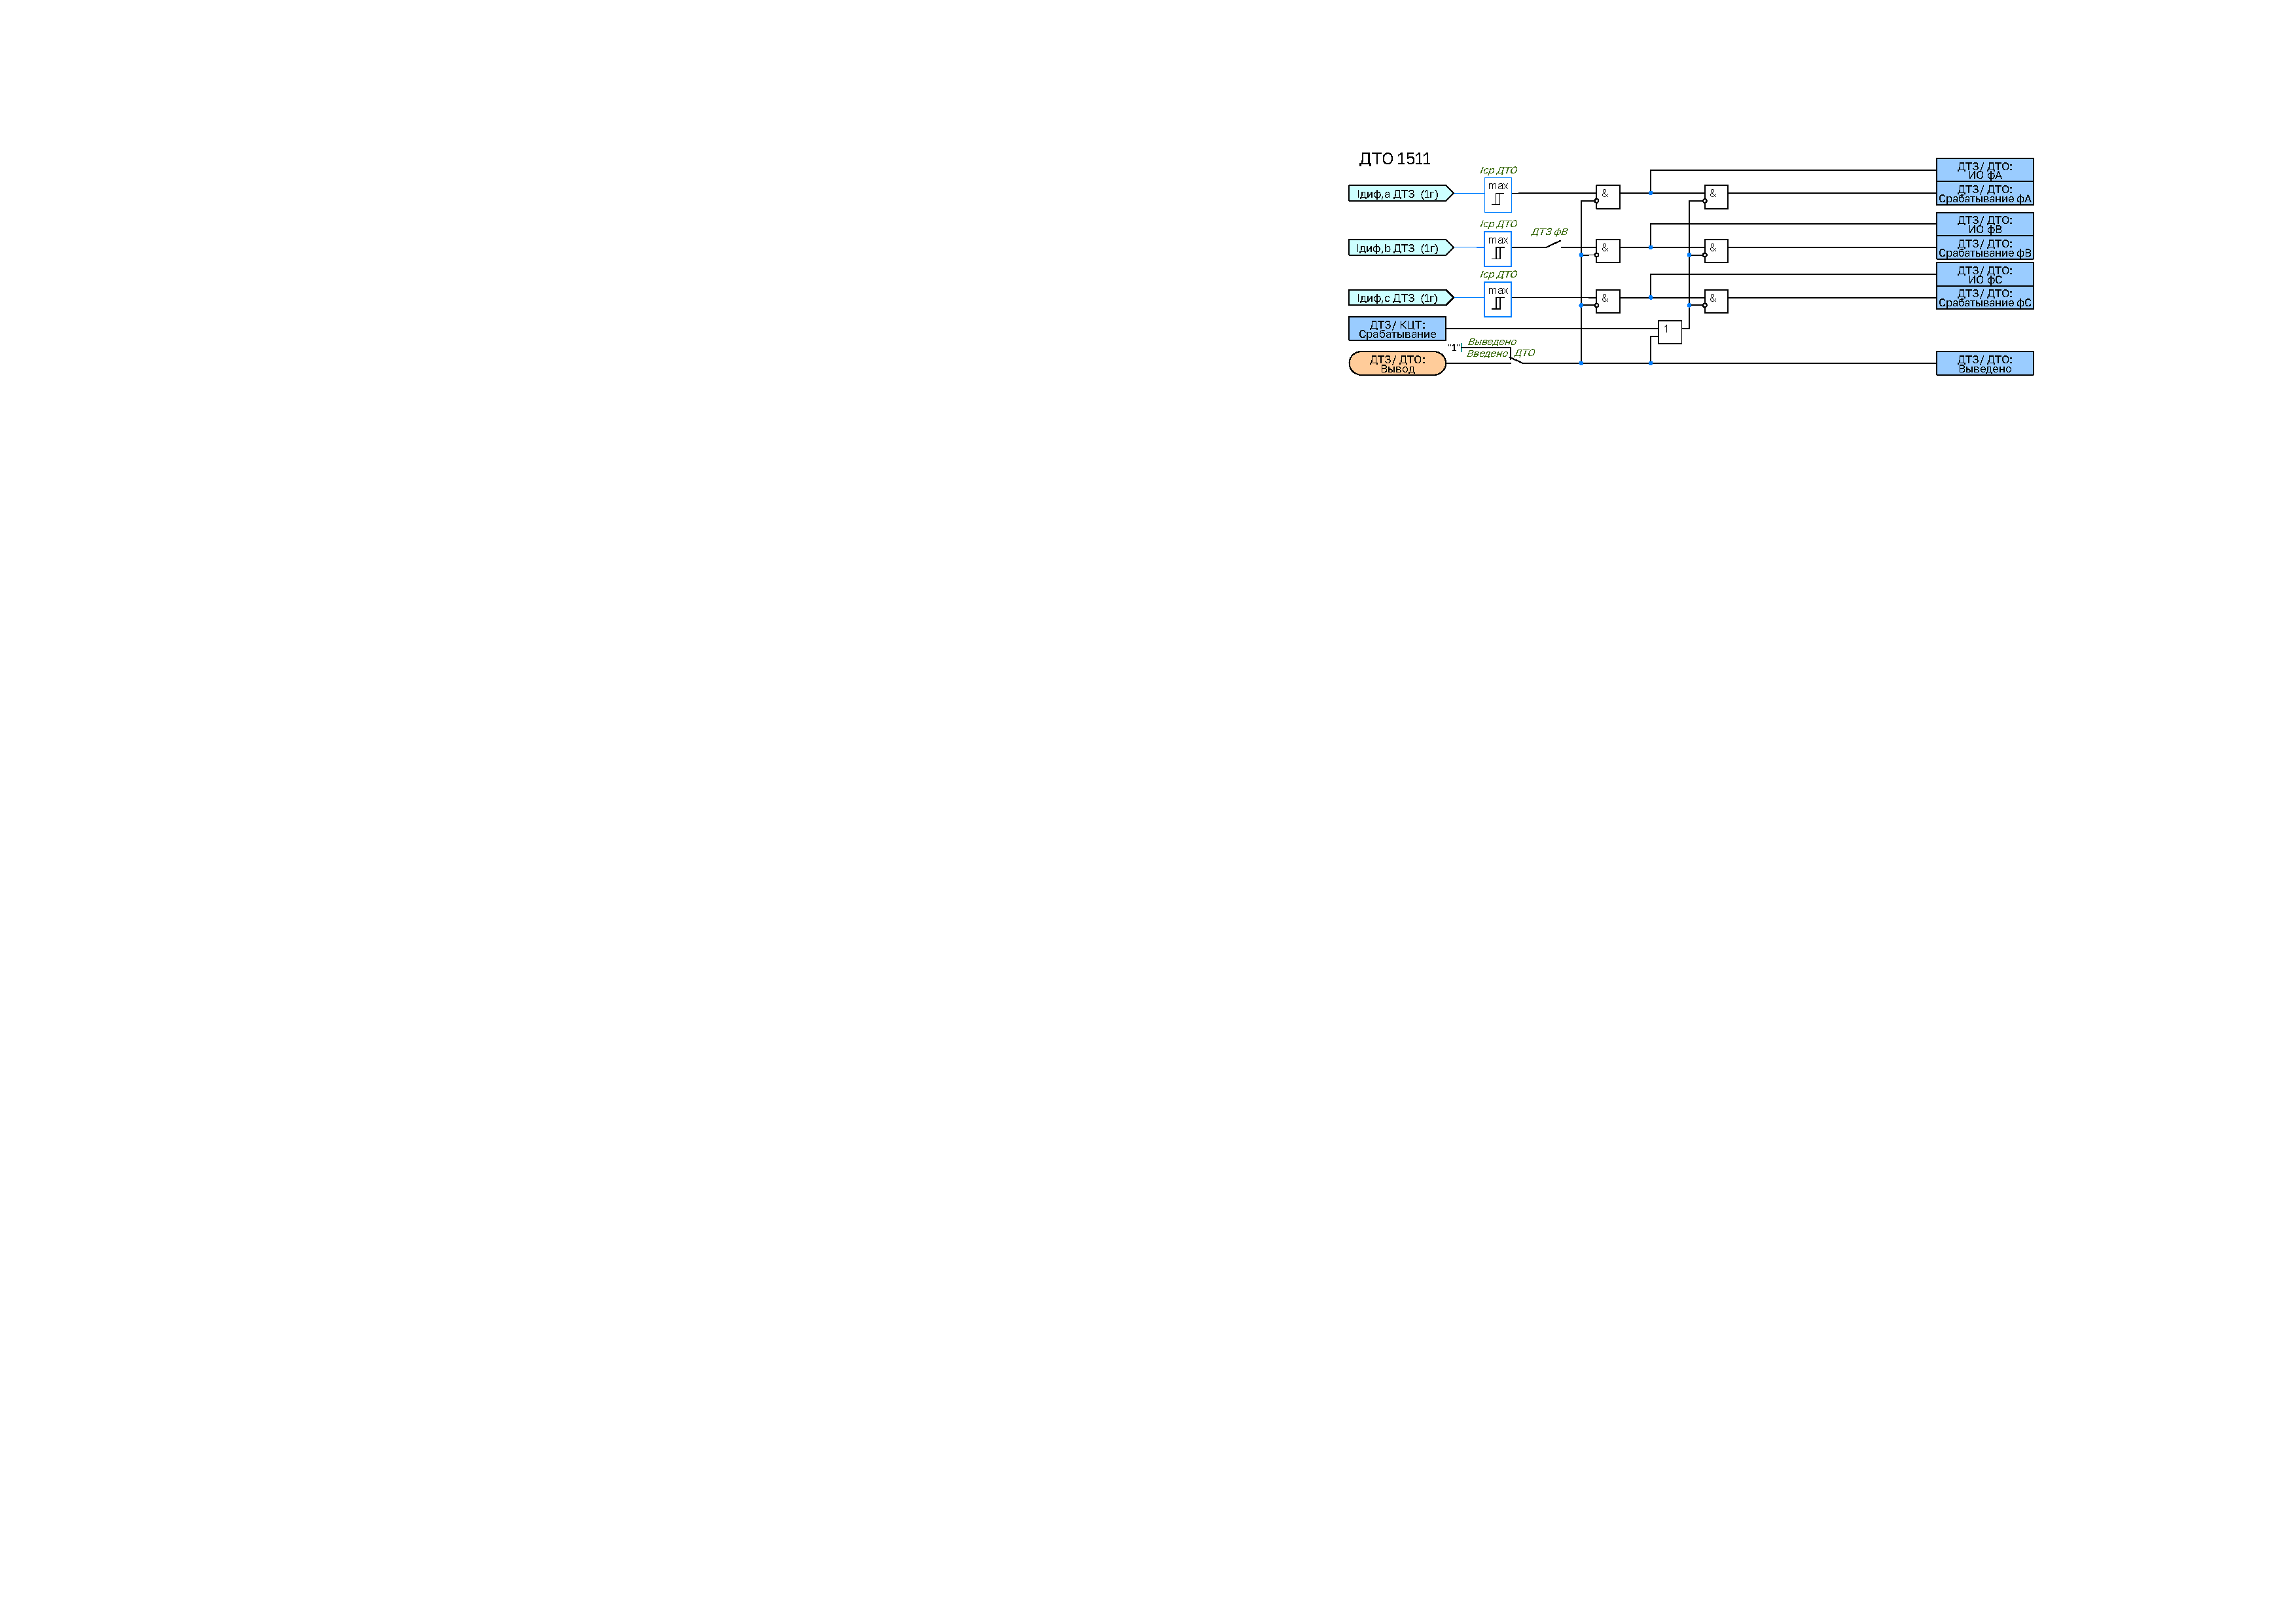
\includegraphics[width=1\textwidth,height=1\textheight,keepaspectratio]{img3.pdf}
\captionof{figure}{Функциональная схема логики дифференциальной токовой отсечки (ДТО)}\label{pict:DTO}
\end{figure}

\item
Ступень дифференциальной защиты с торможением предназначена для защиты от повреждений, сопровождающихся малыми дифференциальными токами, и имеет характеристику срабатывания, состоящую из трех участков (рис.\ref{pict:dz_har}).

\begin{figure}[H]
\centering
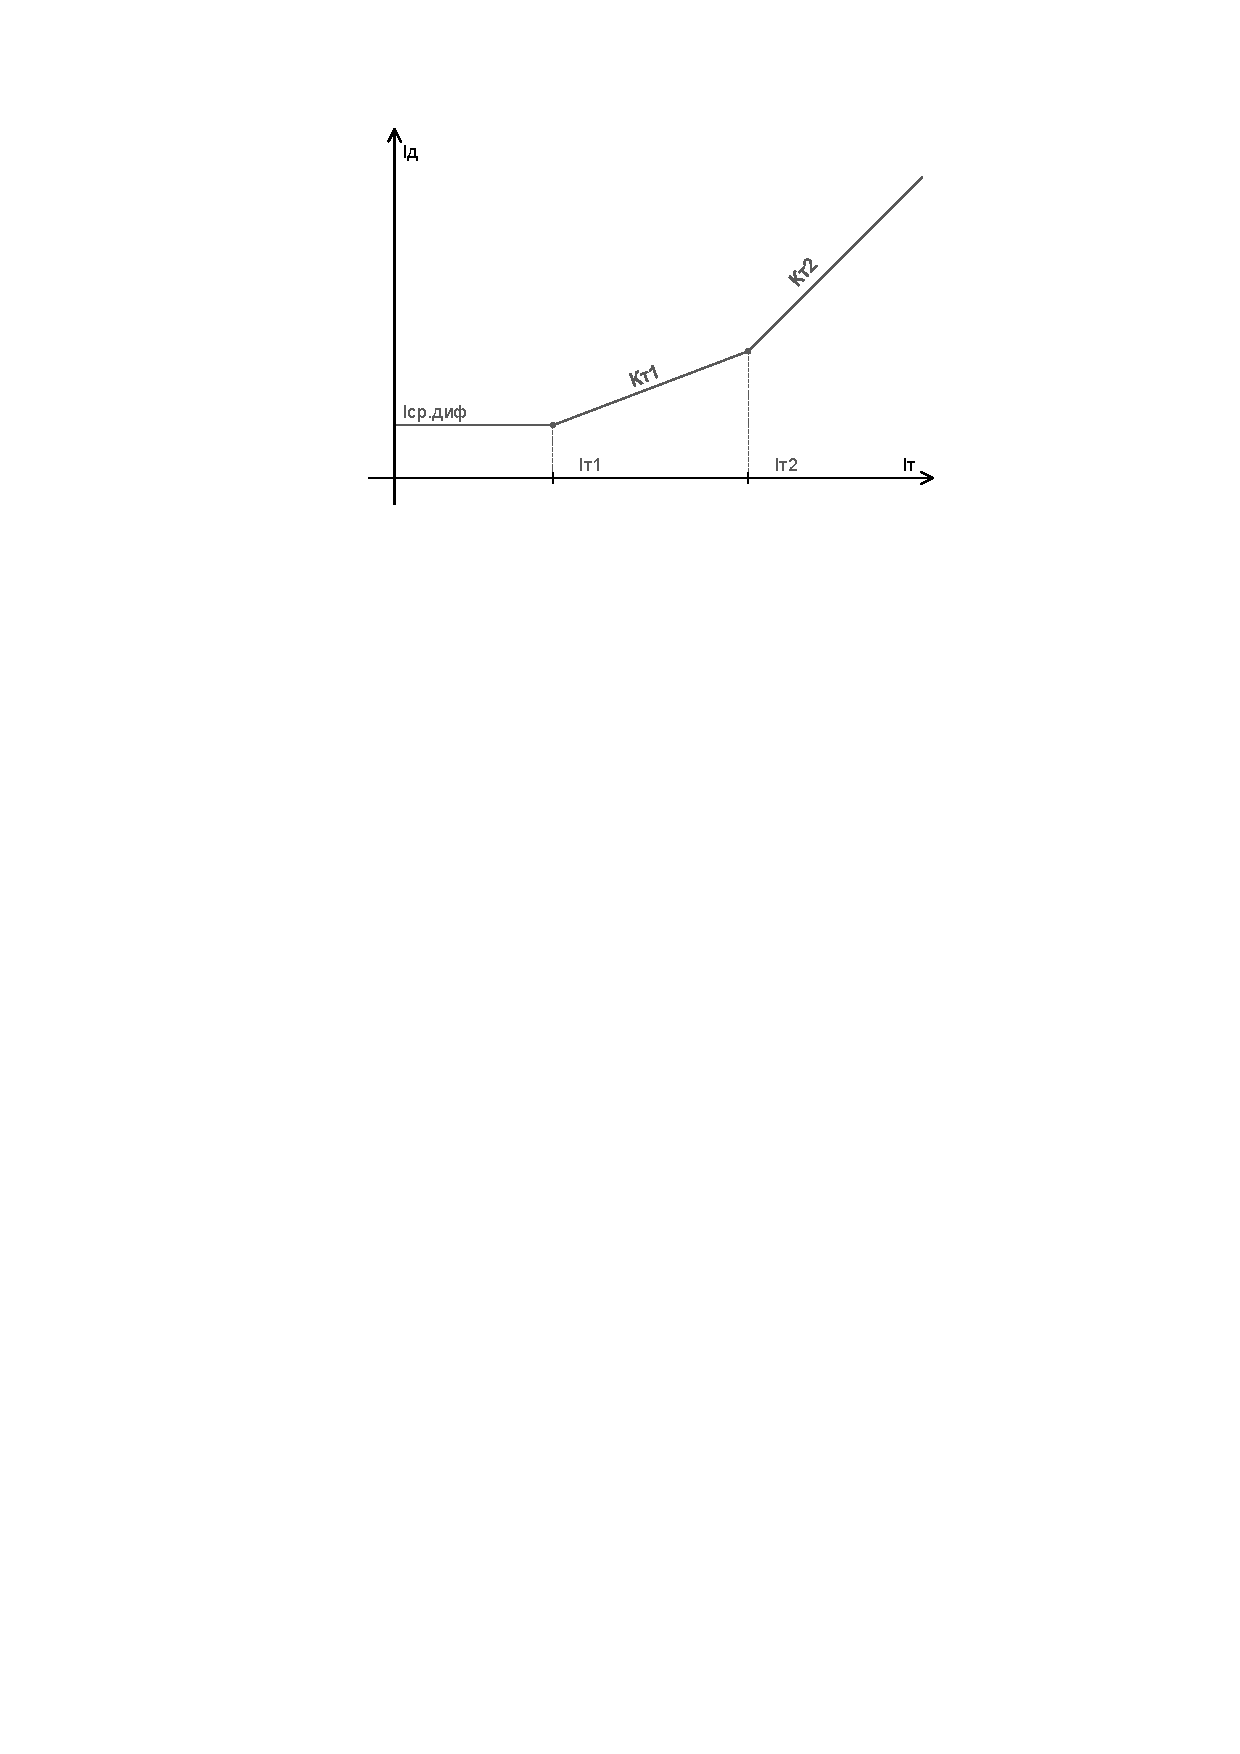
\includegraphics[width=0.5\textwidth,height=0.5\textheight,keepaspectratio]{img4.pdf}
\captionof{figure}{Характеристика срабатывания дифференциальной защиты}\label{pict:dz_har}
\end{figure}

\item
Характеристика торможения дифференциальной защиты задается следующими параметрами:
\begin{itemize}
    \item \textbf{Iср диф. } – минимальный дифференциальный ток срабатывания;
    \item \textbf{Iт1} – начальный ток торможения второго участка;
    \item \textbf{Кт2} – коэффициент наклона второго участка;
    \item \textbf{Iт2} – начальный ток торможения третьего участка;
    \item \textbf{Кт2} – коэффициент наклона третьего участка.
\end{itemize}

\item
Выходной сигнал срабатывания характеристики торможения на соответствующем участке определяется по формулам: 

\begin{itemize}
    \item участок 1: $I_{\textsl{Д}} \geq I_{\textsl{ср.диф}}$, при $I_{\textsl{Т}} \leq I_{\textsl{Т1}}$
    \item участок 2: $I_{\textsl{Д}} \geq I_{\textsl{ср.диф}} + K_{\textsl{Т1}} \cdot (I_{\textsl{Т}} - I_{\textsl{Т1}})$, при $I_{\textsl{Т1}} < I_{\textsl{Т}} \leq I_{\textsl{Т2}}$
    \item участок 3: $I_{\textsl{Д}} \geq I_{\textsl{ср.диф}} + K_{\textsl{Т1}} \cdot (I_{\textsl{Т2}} - I_{\textsl{Т1}}) + K_{\textsl{Т2}} \cdot (I_{\textsl{Т}} - I_{\textsl{Т2}}) $, при $I_{\textsl{Т}} > I_{\textsl{Т2}}$
\end{itemize}

\item
Алгоритм работы ДТО приведен на рисунке \ref{pict:DTZ}.

\vspace{2mm}
\begin{figure}[H]
\centering
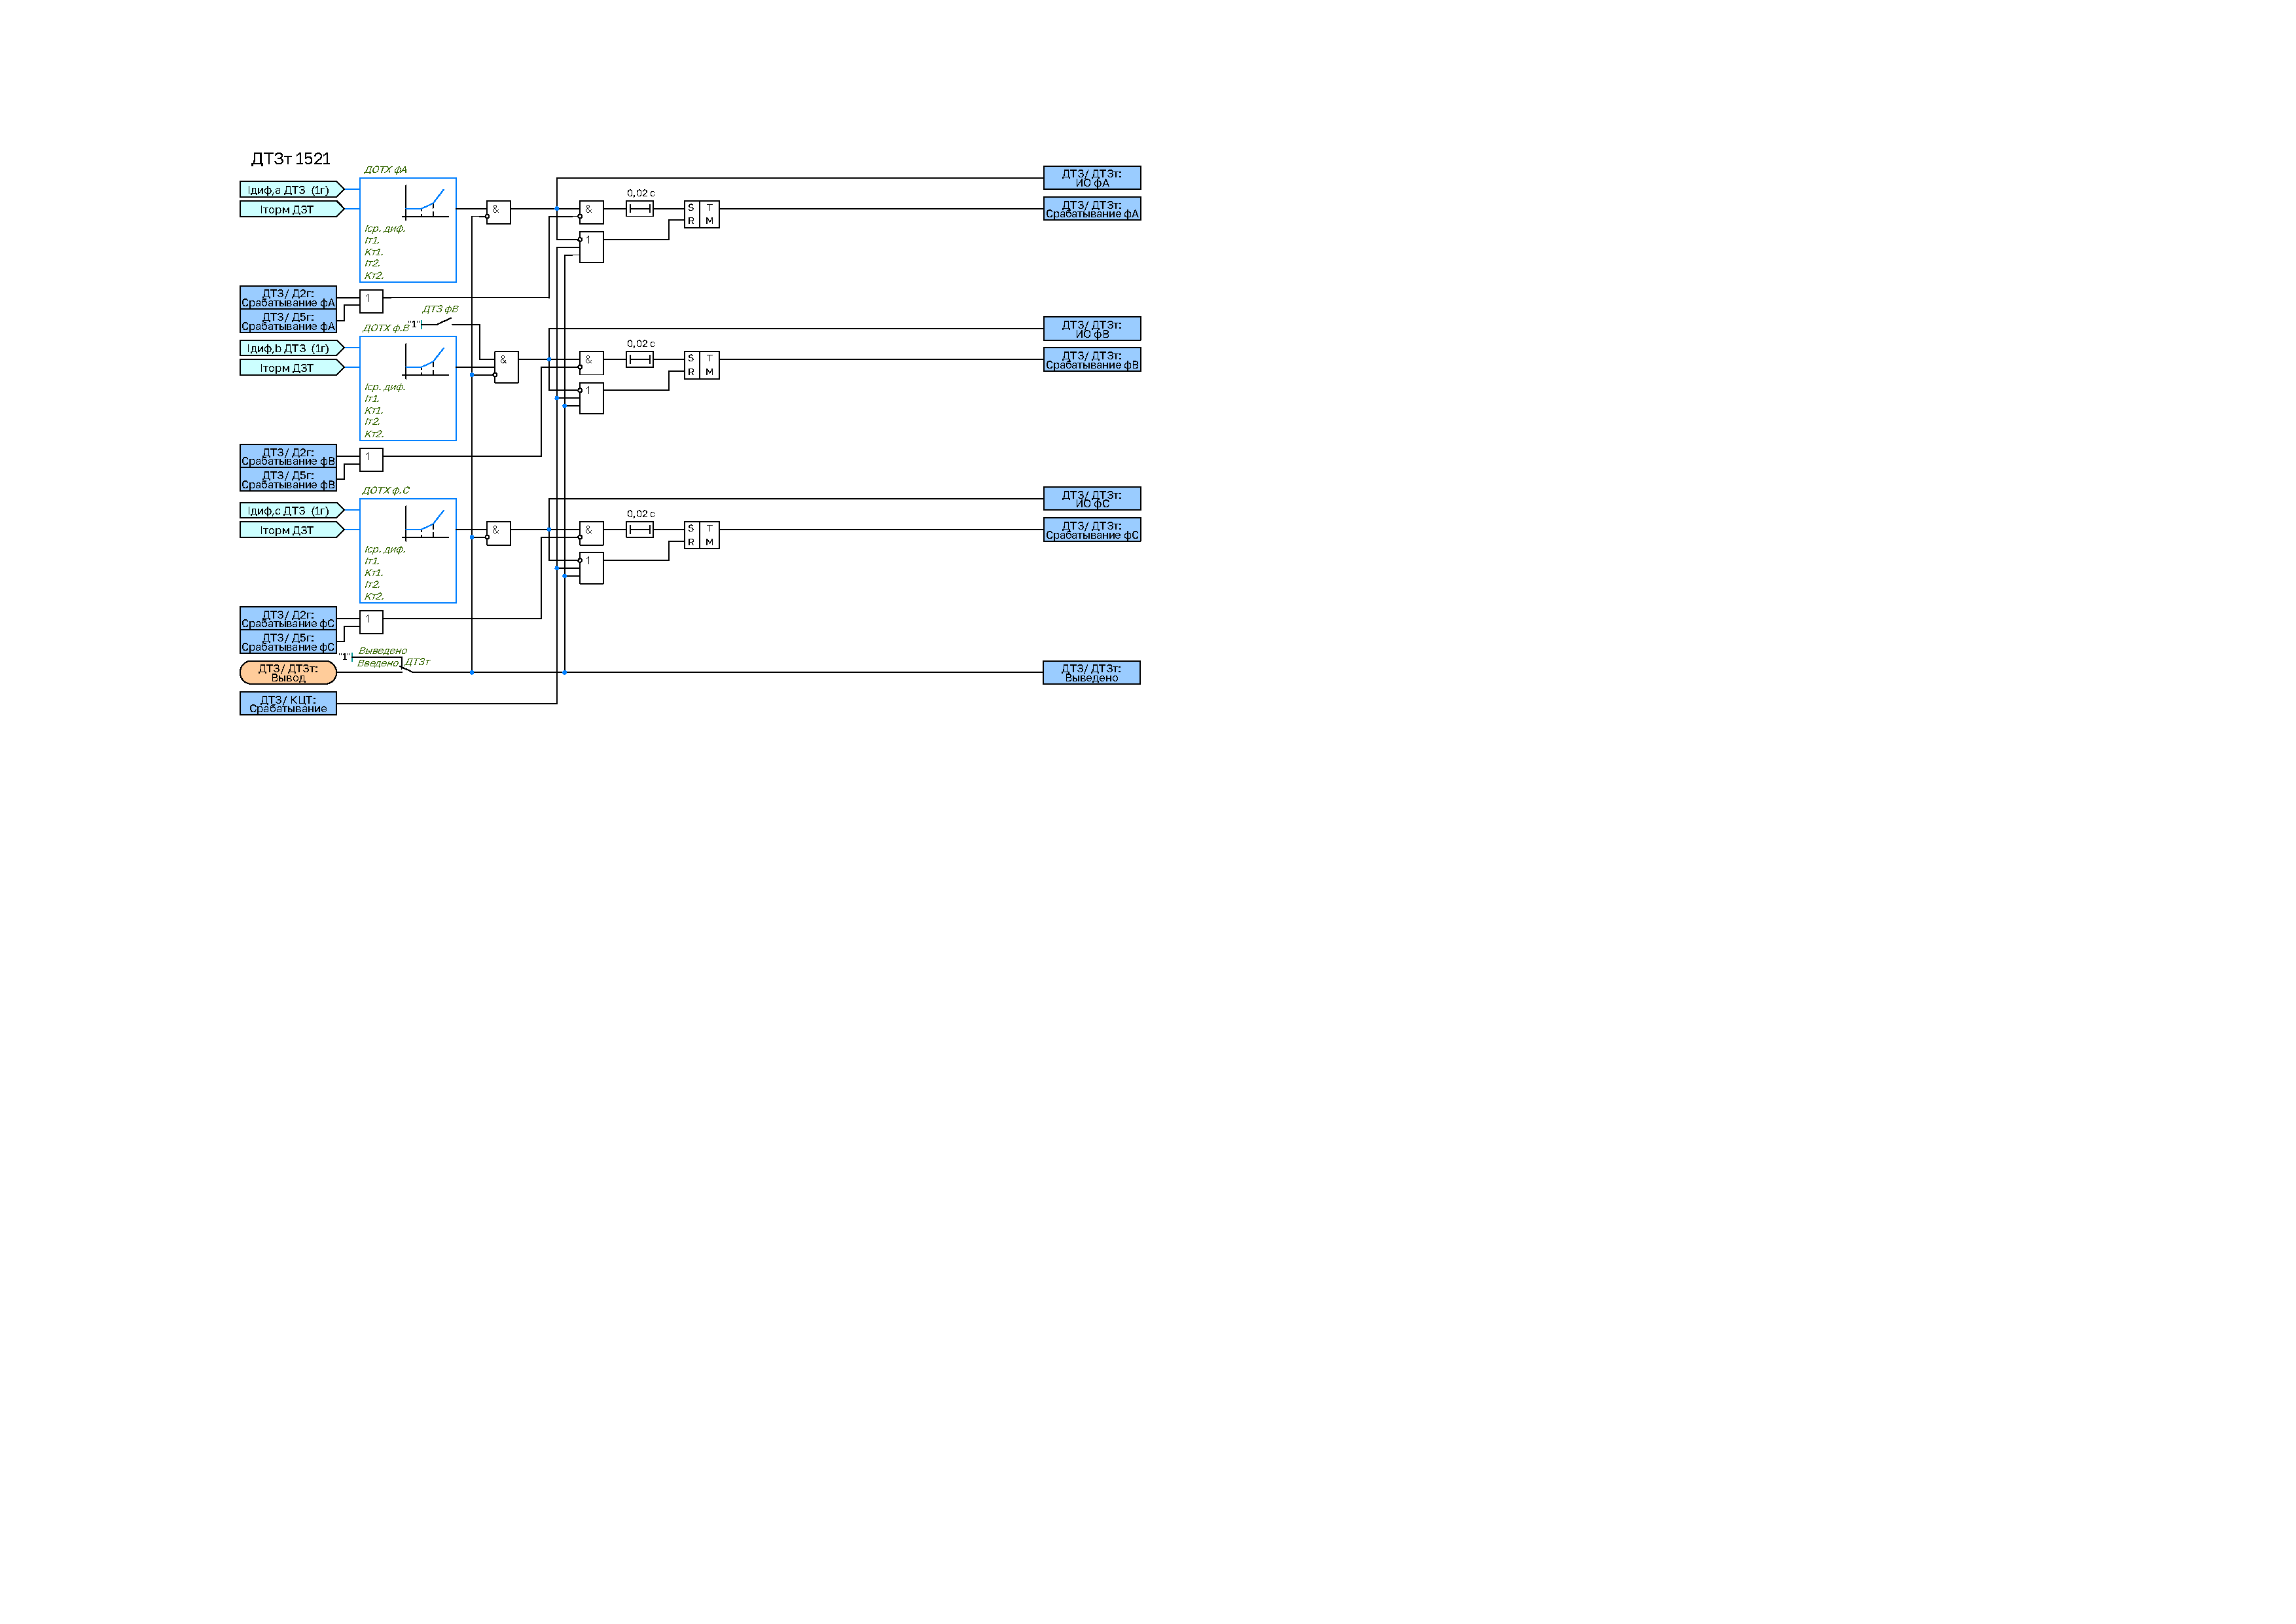
\includegraphics[width=1\textwidth,height=1\textheight,keepaspectratio]{img5.pdf}
\captionof{figure}{Функциональная схема логики дифференциального органа с торможением (ДТЗт)}\label{pict:DTZ}
\end{figure}

\end{enumerate}

\subsubsection{Блокировка по второй гармонике}

\begin{enumerate}[label=\arabic{section}.\arabic{subsection}.\arabic{subsubsection}.\arabic*,  align=left, labelsep=4pt, leftmargin=0pt, itemindent=57pt]

\item
Причиной возникновений броска тока намагничивания в силовом оборудовании (трансформаторах, шунтирующих реакторах) является резкое изменение уровня напряжения намагничивания, характерное для режимов постановки оборудования под напряжение, восстановления уровня напряжения после отключения внешнего КЗ и др. Обнаружение режима броска тока намагничивания основано на контроле отношения величины второй гармоники дифференциального тока, как наиболее характерной для режима броска тока намагничивания, к величине составляющей первой гармоники. 

\item
Ввод блокировки в работу осуществляется программной накладкой \textbf{«Блок.2г.ДТЗт»}. Уровень второй гармоники, при котором производится блокировка дифференциальной защиты с торможением, задается значением \textbf{«I2г/I1г ДТЗт»}. 

\item
Блокировка по второй гармонике выполнена пофазной. В некоторых случаях при броске тока намагничивания содержание второй гармоники в одной из фаз может быть недостаточно большим, что может вызвать ложное срабатывание защиты. Для данных случаев может быть использована перекрестная блокировка по 2ой гармонике. Перекрестная блокировка по 2ой гармонике действует на блокирование всех фаз при превышении заданного уровня второй гармоники в одной или в двух фазах в зависимости от положения программной накладки \textbf{«Перекр.блок.2г»}. Перекрестная блокировка по 2ой гармонике выполняется в течение ограниченного времени, определяемого параметром \textbf{«Тперекр.блок.2г»}. Алгоритм работы Д2Г приведен на рисунке \ref{pict:d2g}.

\vspace{2mm}
\begin{figure}[H]
\centering
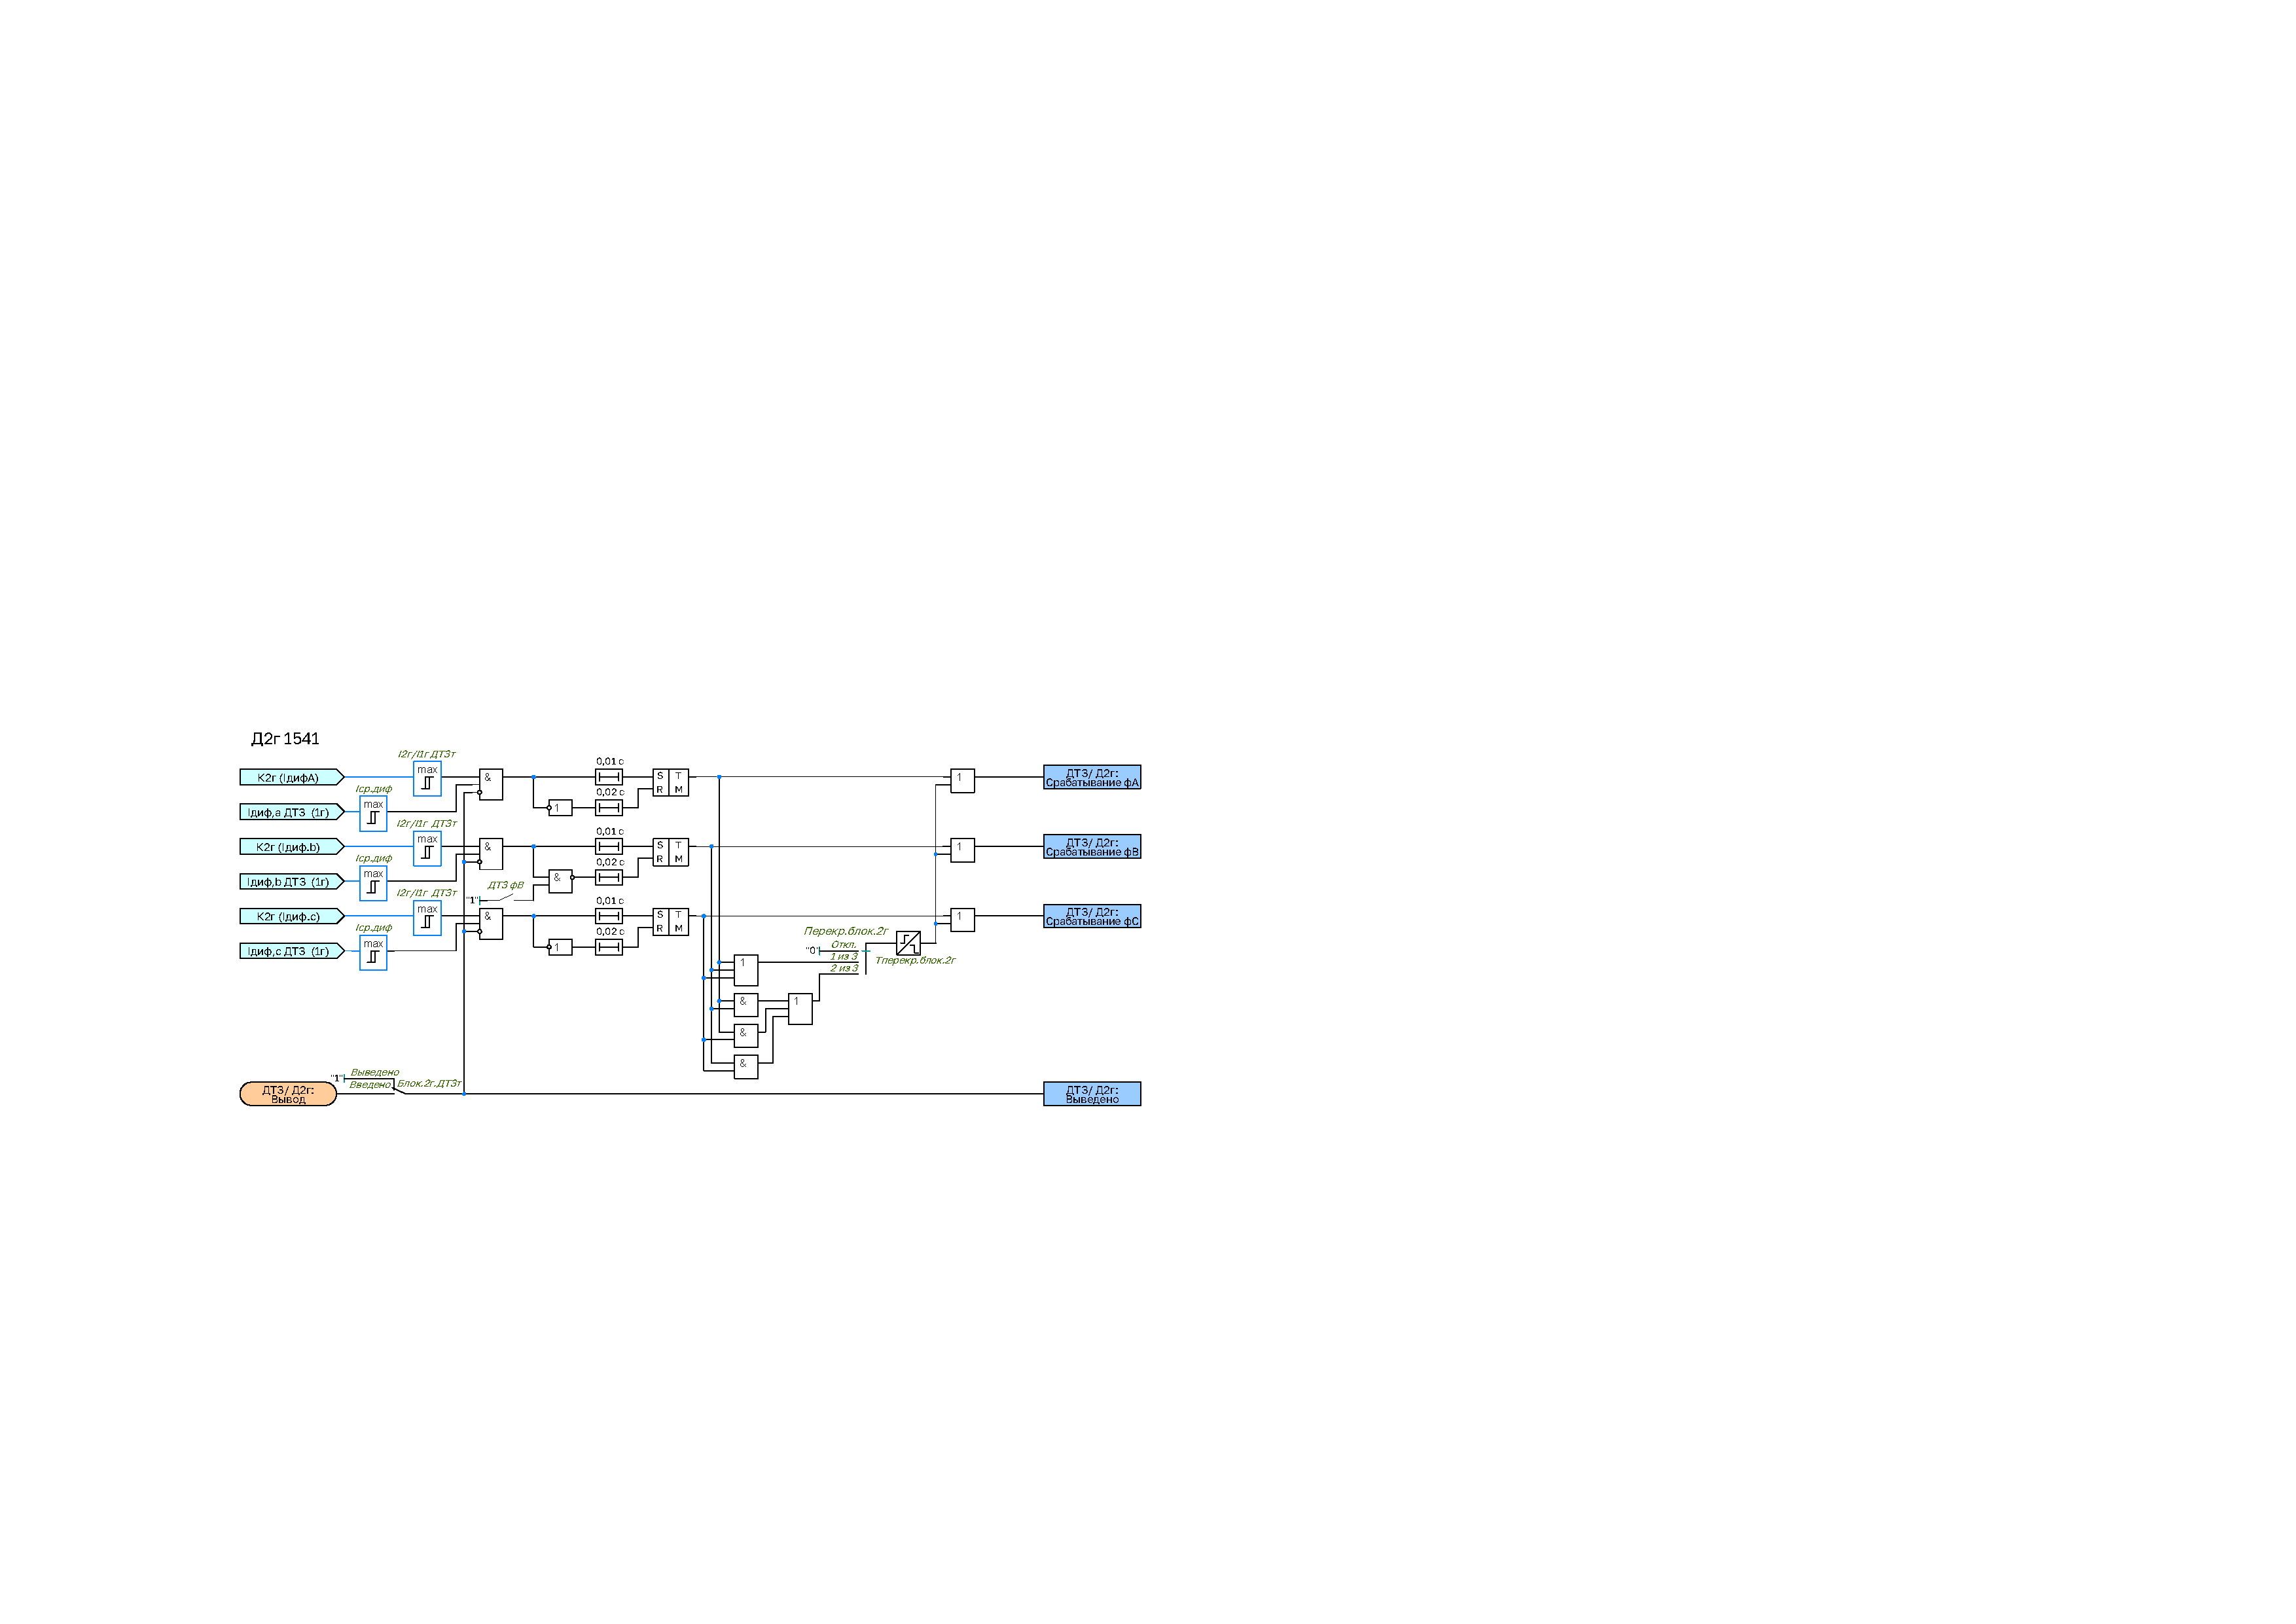
\includegraphics[width=1\textwidth,height=1\textheight,keepaspectratio]{img6.pdf}
\captionof{figure}{Функциональная схема логики блока блокировки по 2 гармонике}\label{pict:d2g}
\end{figure}

\end{enumerate}

\subsubsection{Блокировка по пятой гармонике}

\begin{enumerate}[label=\arabic{section}.\arabic{subsection}.\arabic{subsubsection}.\arabic*,  align=left, labelsep=4pt, leftmargin=0pt, itemindent=57pt]

\item
Причиной возникновений повышенной индукции силовых трансформаторов является повышение напряжения и/или понижение уровня частоты. Повышение индукции выше номинального значения быстро ведет к насыщению стального сердечника и большим потерям от вихревых токов. Обнаружение режима перенасыщения основано на контроле отношения величины составляющей пятой гармоники дифференциального тока, как наиболее характерной для режима перенасыщения, к величине составляющей первой гармоники. 

\item
Ввод блокировки в работу осуществляется программной накладкой \textbf{«Блок.5г.ДТЗт»}. Уровень пятой гармоники, при котором производится блокировка дифференциальной защиты с торможением, задается значением \textbf{«I5г/I1г ДТЗт»}. 

\item
Блокировка по пятой гармонике выполнена пофазной. В некоторых случаях содержание пятой гармоники в одной из фаз может быть недостаточно большим, что может вызвать ложное срабатывание защиты. Для данных случаев может быть использована перекрестная блокировка по 5ой гармонике. Перекрестная блокировка по 5ой гармонике действует на блокирование всех фаз при превышении заданного уровня пятой гармоники в одной или в двух фазах в зависимости от положения программной накладки \textbf{«Перекр.блок.5г»}. Перекрестная блокировка по 5ой гармонике выполняется в течение ограниченного времени, определяемого параметром \textbf{«Тперекр.блок.5г»}. Алгоритм работы Д2Г приведен на рисунке \ref{pict:d5g}.

\vspace{2mm}
\begin{figure}[H]
\centering
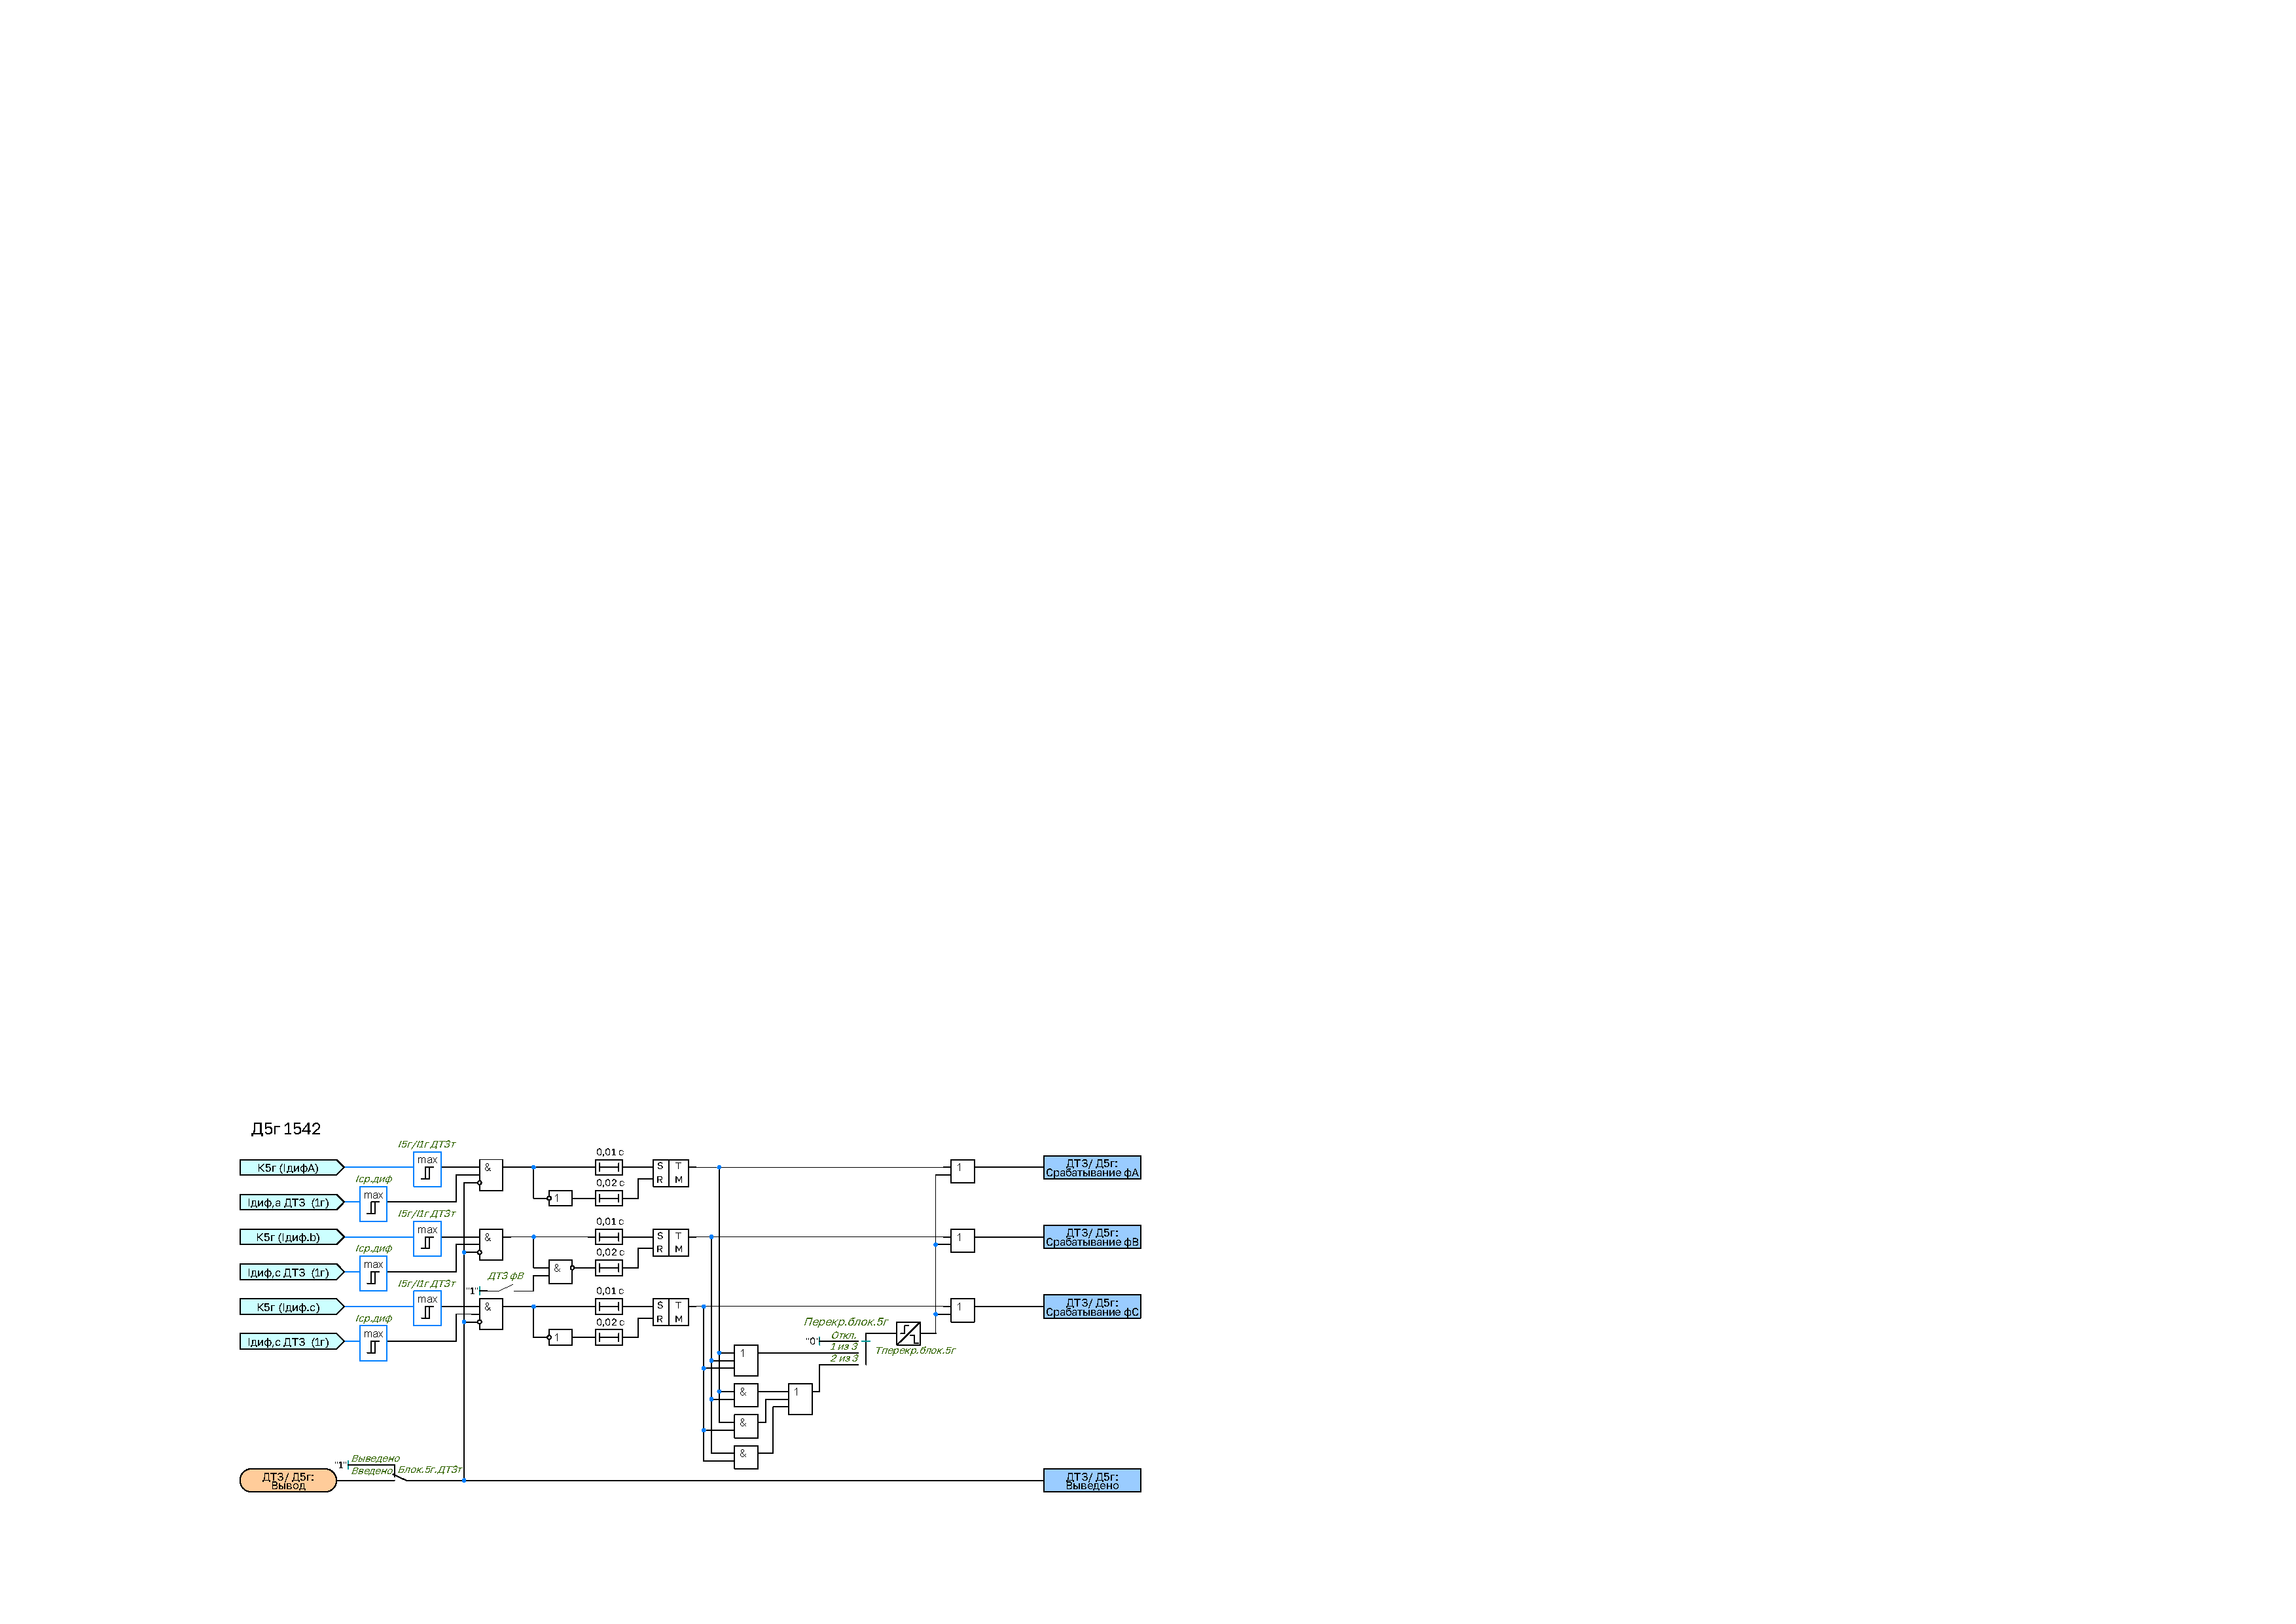
\includegraphics[width=1\textwidth,height=1\textheight,keepaspectratio]{img7.pdf}
\captionof{figure}{Функциональная схема логики блока блокировки по 5 гармонике}\label{pict:d5g}
\end{figure}

\end{enumerate}

\subsubsection{Контроль цепей тока}

\begin{enumerate}[label=\arabic{section}.\arabic{subsection}.\arabic{subsubsection}.\arabic*,  align=left, labelsep=4pt, leftmargin=0pt, itemindent=57pt]

\item
Функция содержит логику контроля исправности измерительных цепей тока. Обнаружение неисправности измерительных цепей осуществляется при превышении дифференциальным током в любой из фаз значения \textbf{«Iнеисп ДТЗ»}. По истечении выдержки времени \textbf{«Тнеисп ДТЗ»} формируется сигнал о неисправности цепей измерения защиты. 

\vspace{2mm}
\begin{figure}[H]
\centering
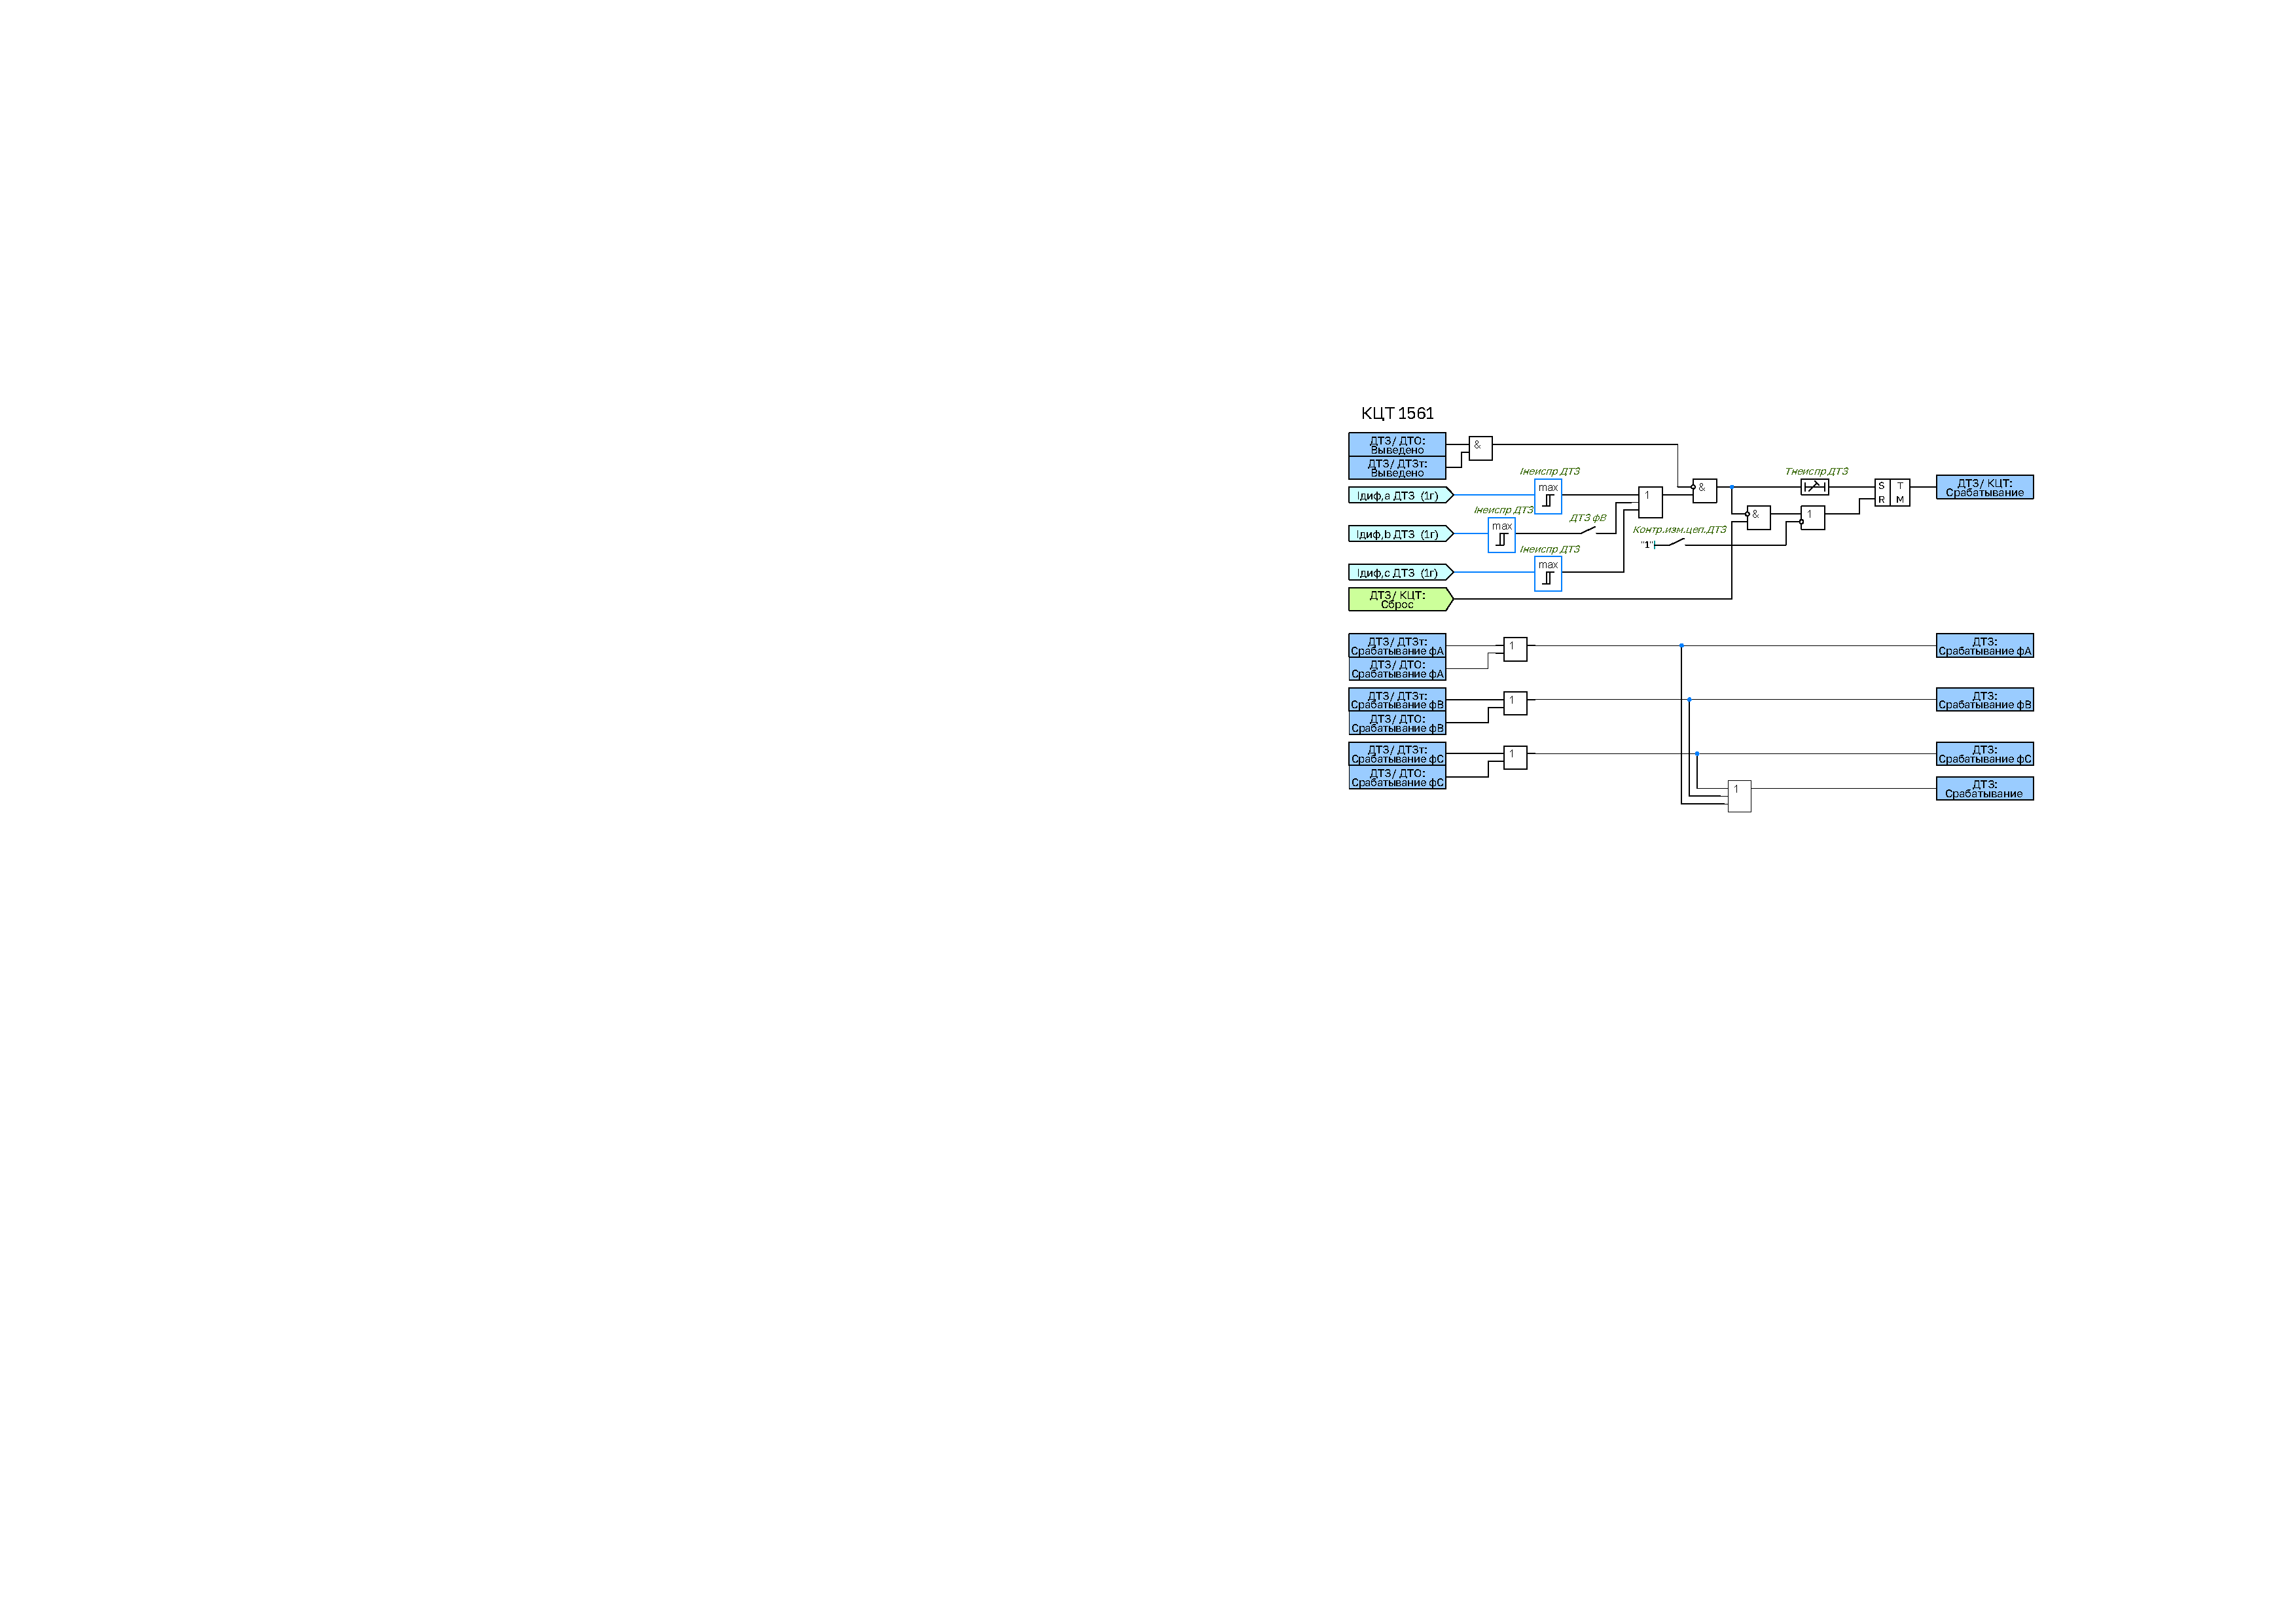
\includegraphics[width=1\textwidth,height=1\textheight,keepaspectratio]{img8.pdf}
\captionof{figure}{Функциональная схема логики блока контроля цепей тока}\label{pict:KCT}
\end{figure}



\end{enumerate}\color{unidarkgreen}{\subsection{Максимальная токовая защита стороны НН}}
\color{black}

\begin{enumerate}[label=\arabic{section}.\arabic{subsection}.\arabic*,  align=left, labelsep=4pt, leftmargin=0pt, itemindent=57pt]

\item
Максимальная токовая защита (МТЗ) стороны НН предназначена для резервирования действия основных быстродействующих защит ошиновки стороны НН. Защита выполнена трехступенчатой (токовая отсечка и две ступени МТЗ). Измерительные цепи защиты включены на токи фаз А, В, С со стороны НН автотрансформатора. Уставки МТЗ НН приведены в таблице \ref{app_set:mtz}.

\item 
Ступень ТО имеет регулируемое значение по току и времени срабатывания. Значение срабатывания по току определяются параметрами \textbf{«Iср ТО НН»}. Задержка на срабатывание защиты задается параметром \textbf{«Тср ТО НН»}. Алгоритм работы токовой отсечки приведен на рисунке \ref{pict:toks}.

\vspace{2mm}
\begin{figure}[H]
\centering
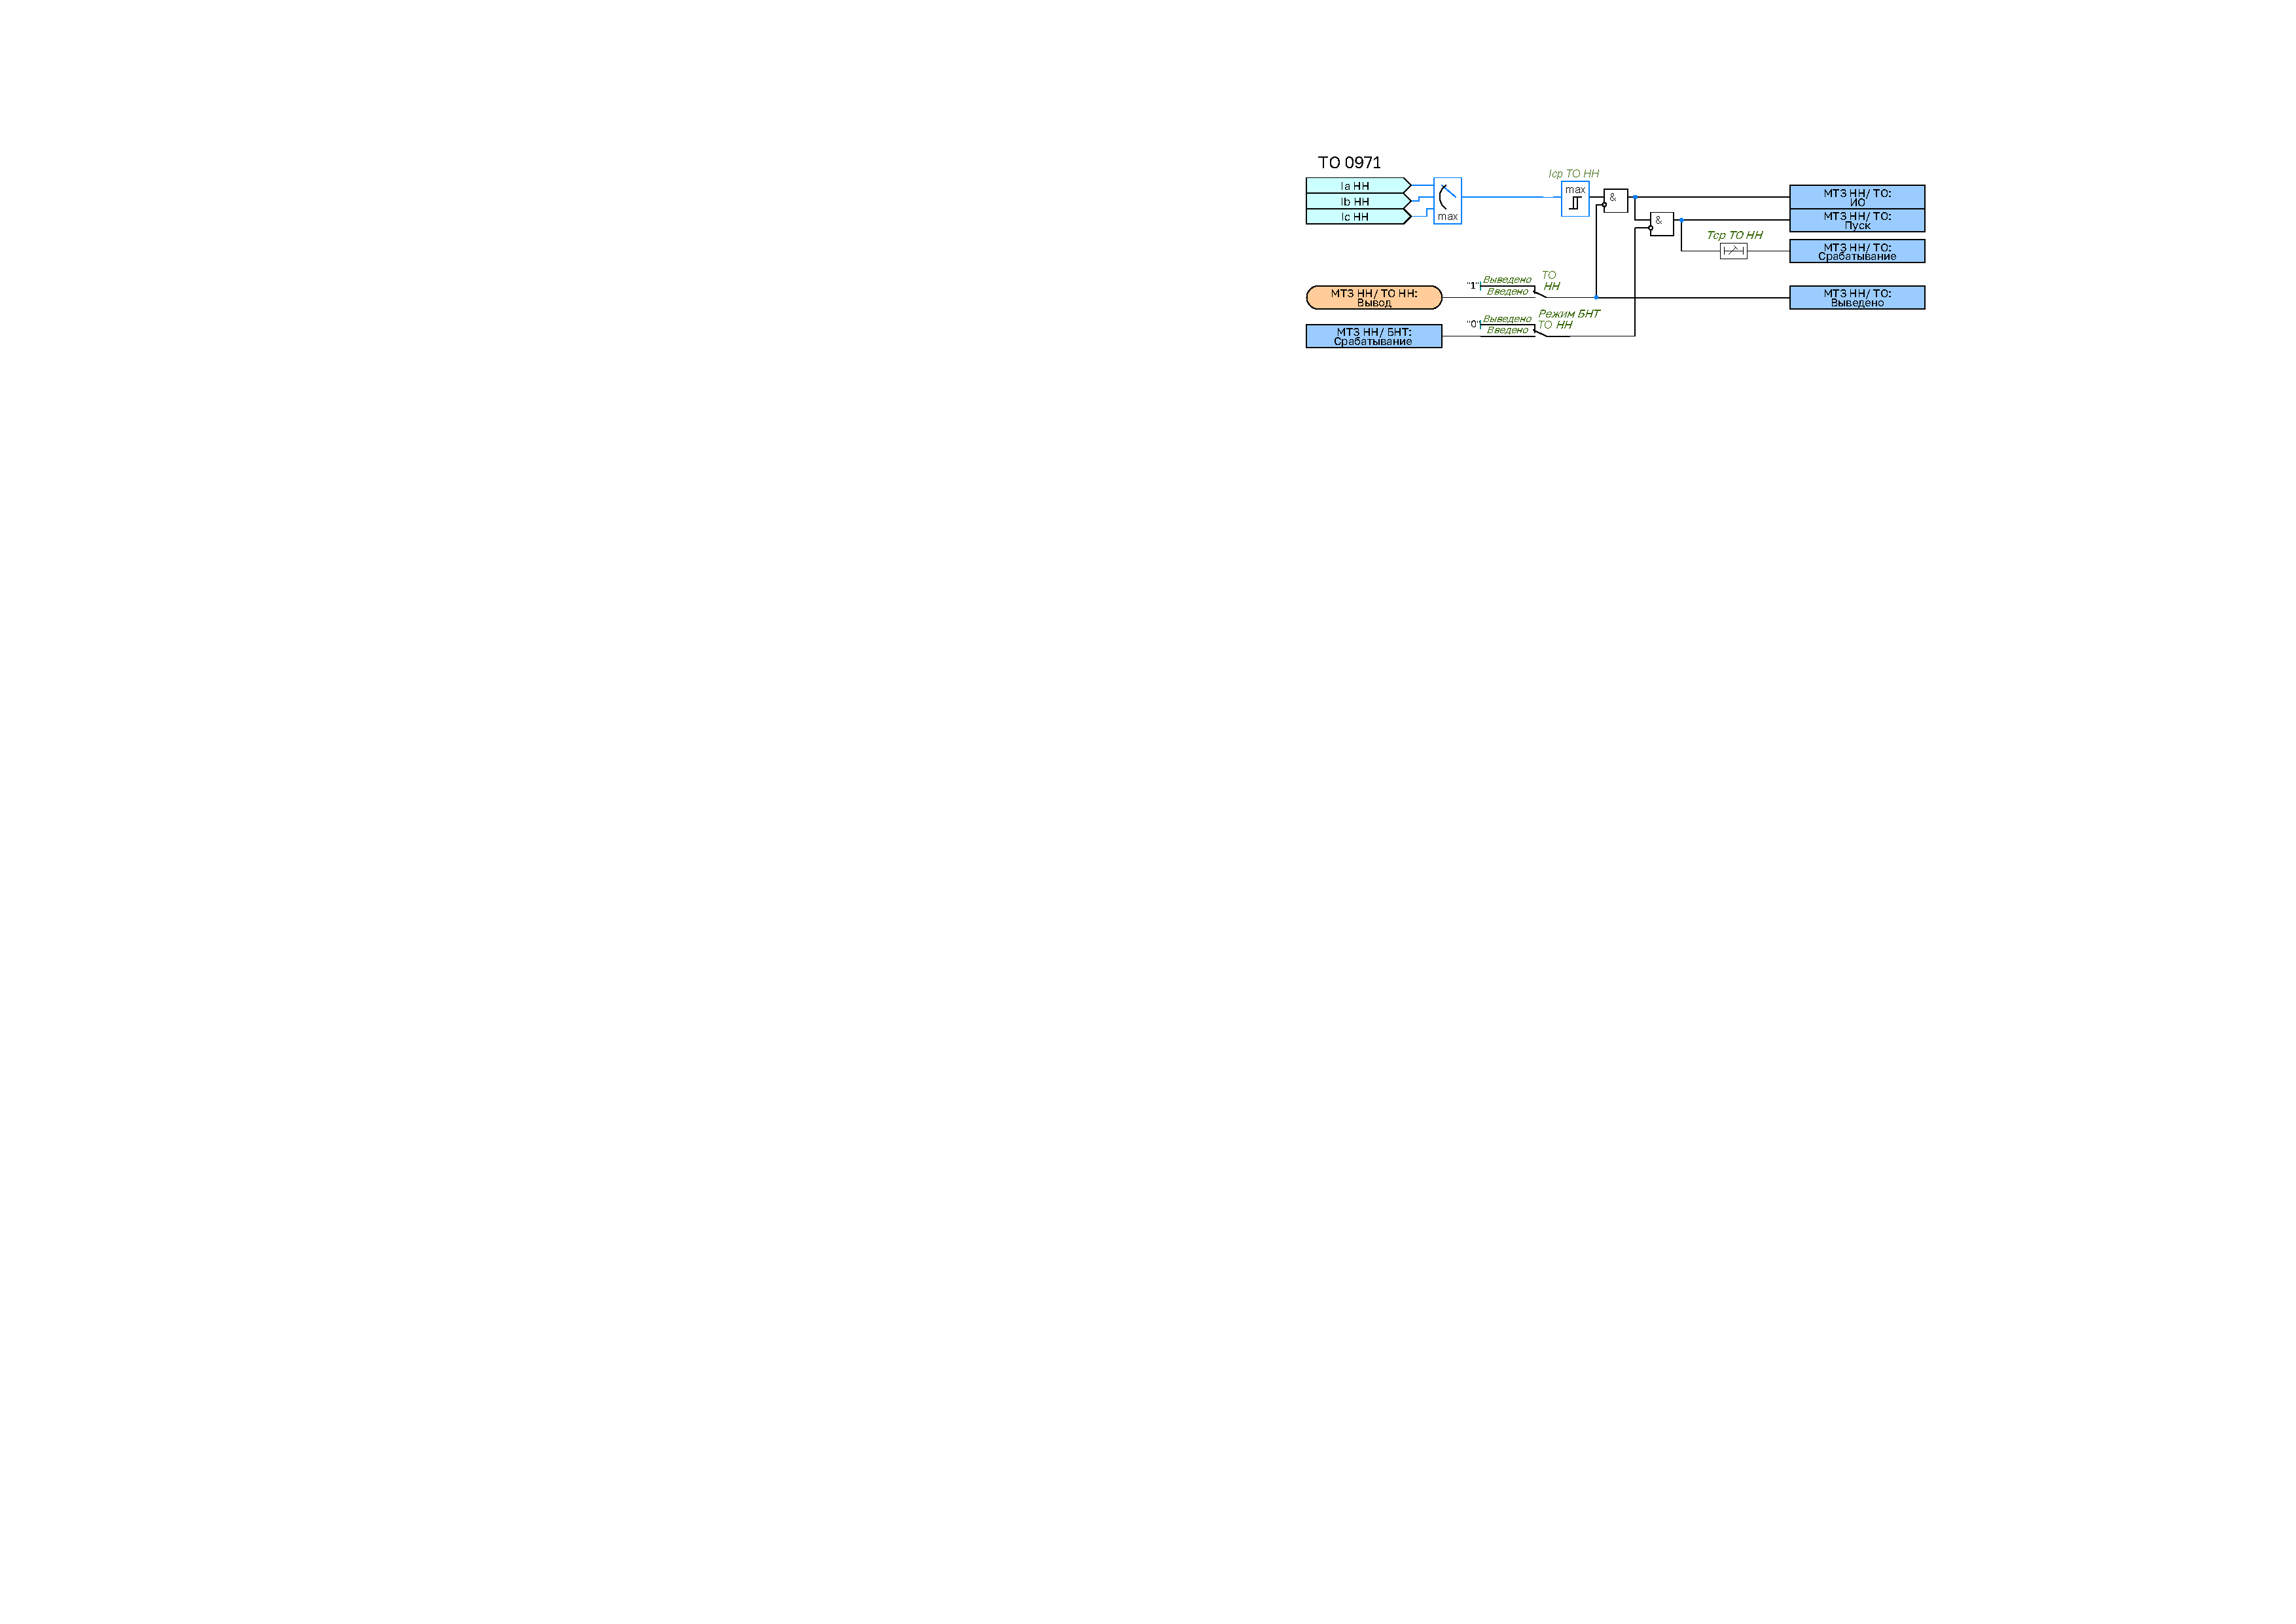
\includegraphics[width=1\textwidth,height=1\textheight,keepaspectratio]{img9.pdf}
\captionof{figure}{Функциональная схема логики токовой отсечки}\label{pict:toks}
\end{figure}

\item
Каждая из ступеней МТЗ имеет регулируемые значения по току и времени срабатывания. Значения срабатывания по току определяются параметрами \textbf{«Iср МТЗ-1 НН»} и \textbf{«Iср МТЗ-2 НН»} для первой и второй ступеней соответственно. Задержки на срабатывание защиты задаются параметрами \textbf{«Тср МТЗ-1 НН»} и \textbf{«Тср МТЗ-2 НН»}.

\item
Каждая из ступеней защиты может выполнена с пуском по напряжению. Ввод контроля пуска по напряжению в логику работы ступеней осуществляется программными накладками \textbf{«Режим КПОН МТЗ-1 НН»} и  \textbf{«Режим КПОН МТЗ-2 НН»} для первой и второй ступеней соответственно.

\item
Каждая из ступеней защиты может выполнена с блокировкой по второй гармонике (отношению уровня второй гармоники к первой). Данная блокировка реализована на базе модуля «ОВ БНТ». Ввод контроля броска намагничивающего тока выполняется программными накладками \textbf{«Режим БНТ МТЗ-1 НН»}, \textbf{«Режим БНТ МТЗ-2 НН»}. 

\item
Алгоритм работы первой ступени МТЗ приведен на рисунке \ref{pict:mtz1}. Алгоритм работы второй ступени МТЗ выполнен аналогично.

\vspace{2mm}
\begin{figure}[H]
\centering
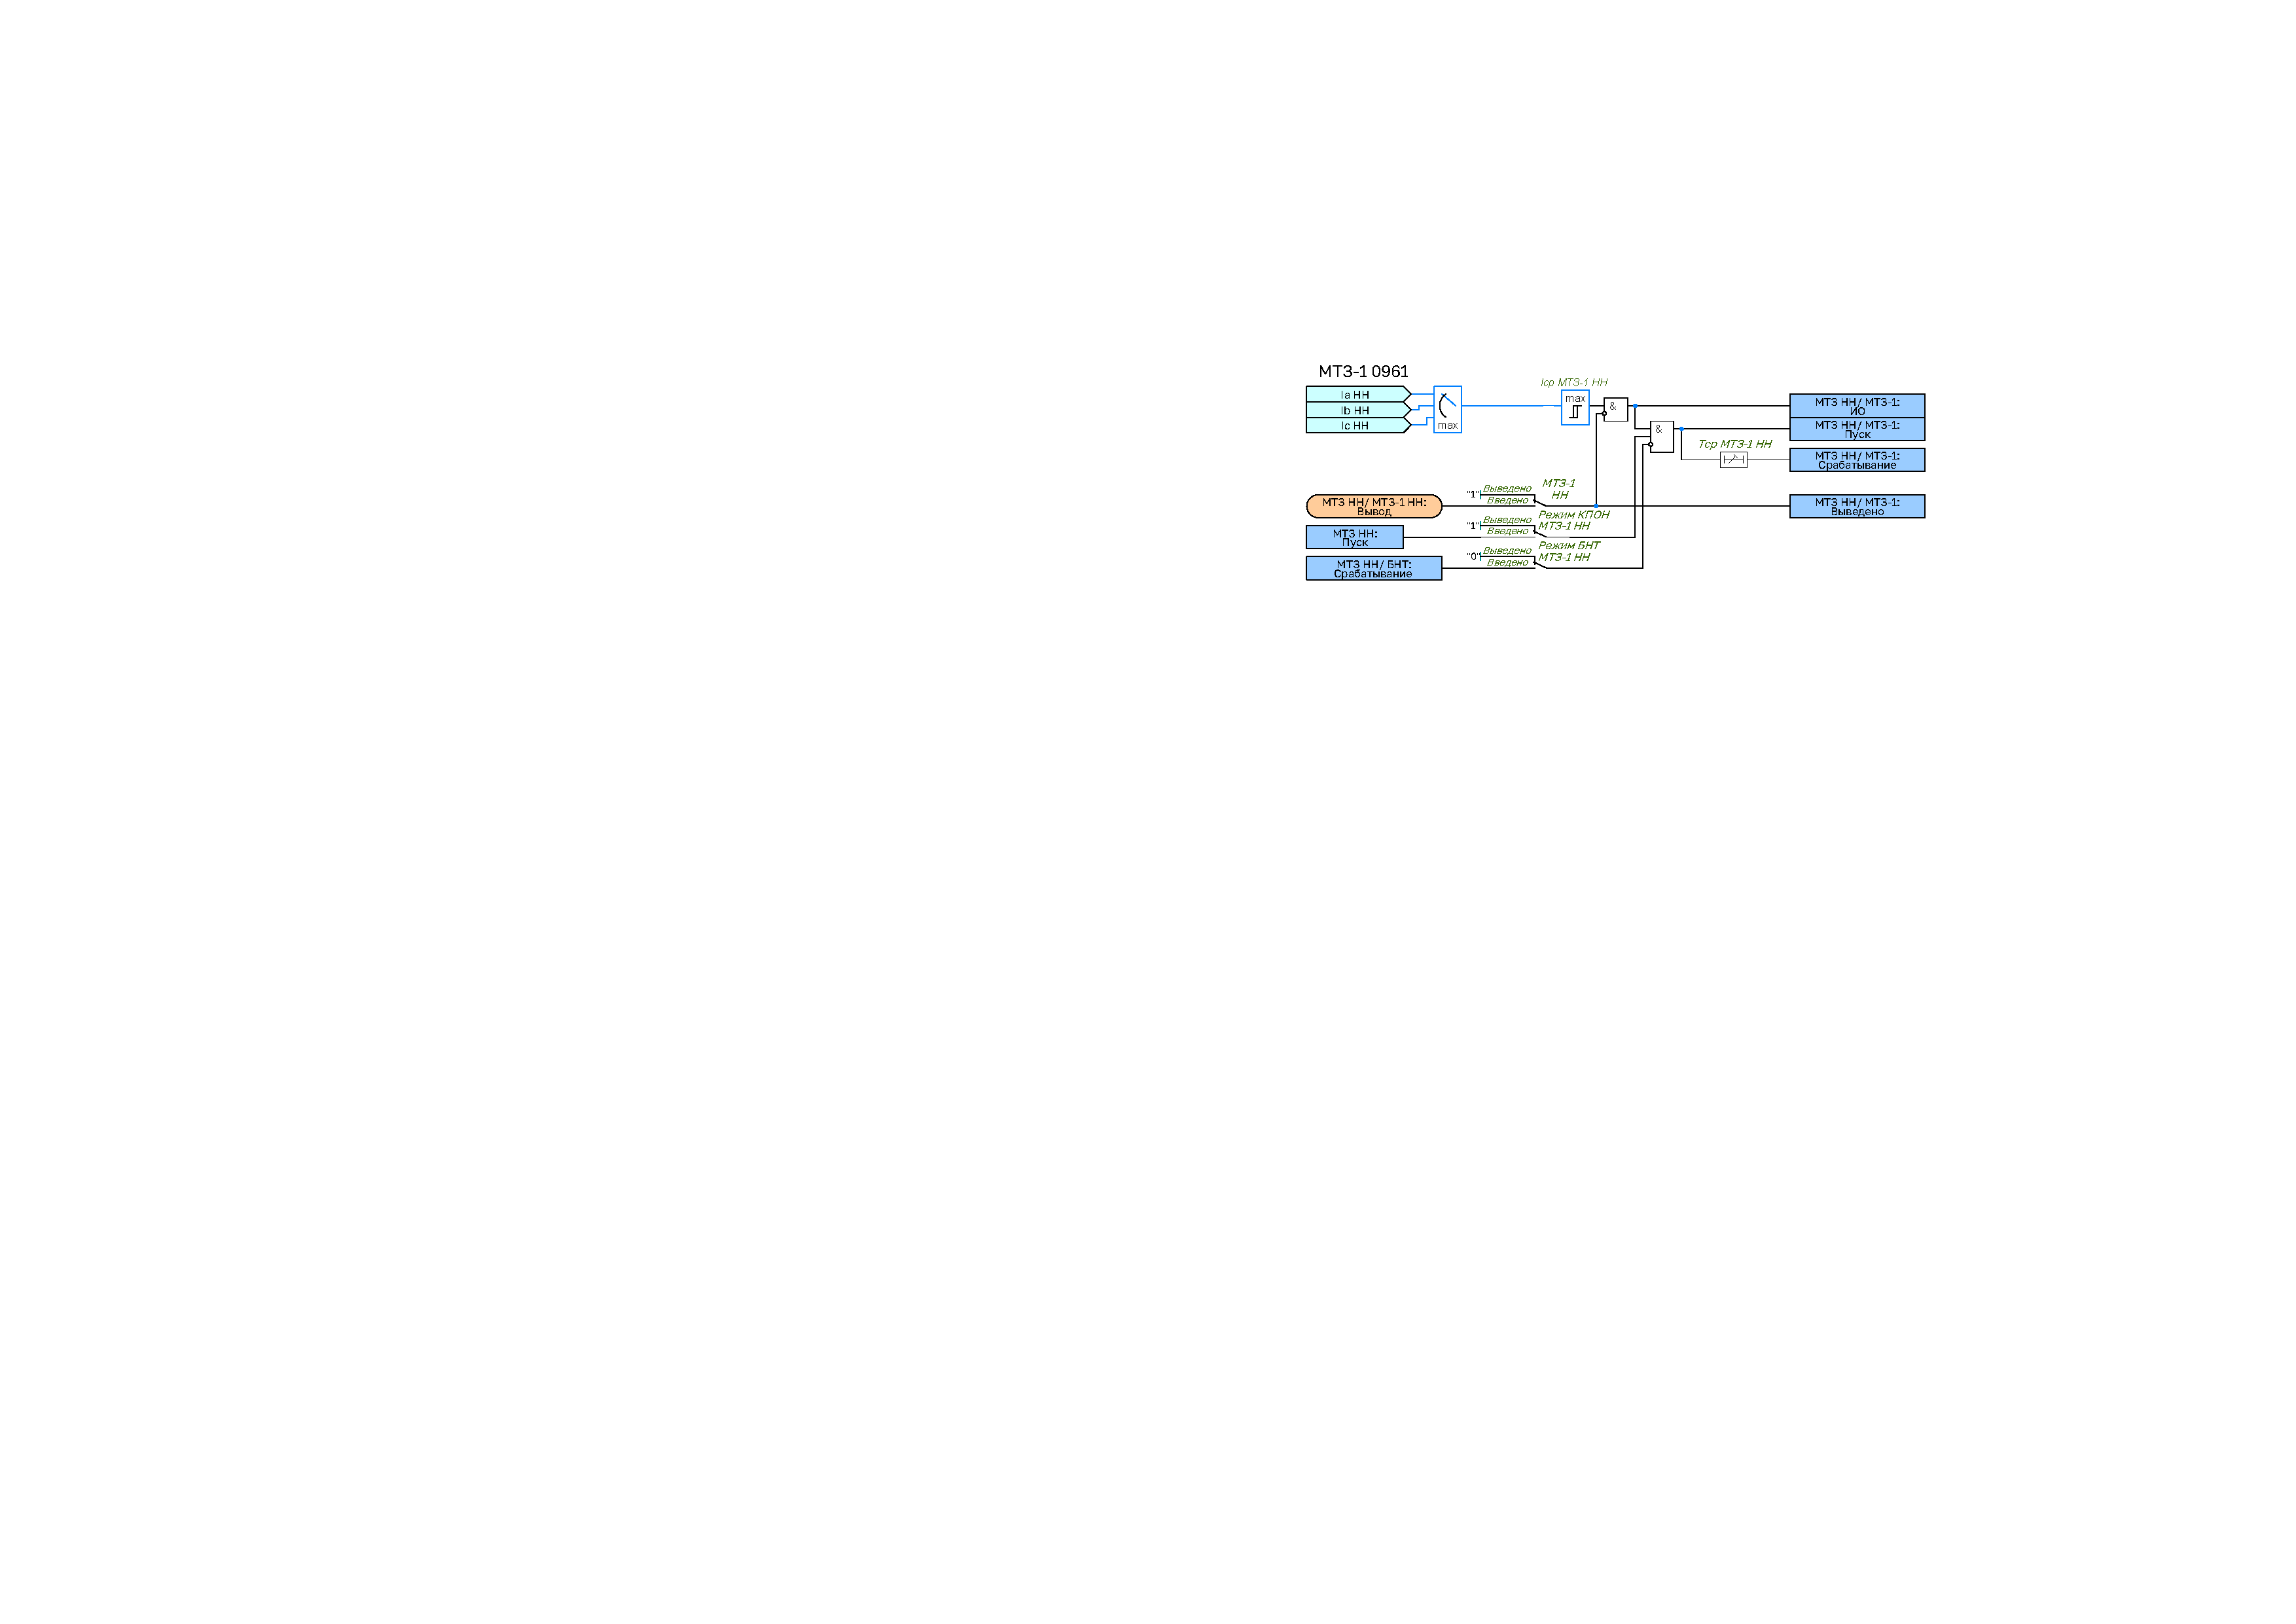
\includegraphics[width=1\textwidth,height=1\textheight,keepaspectratio]{img10.pdf}
\captionof{figure}{Функциональная схема логики первой ступени МТЗ НН}\label{pict:mtz1}
\end{figure}

\item
Алгоритм работы органа выявления БНТ приведен на рисунке \ref{pict:mtz_bnt}. 

\vspace{2mm}
\begin{figure}[H]
\centering
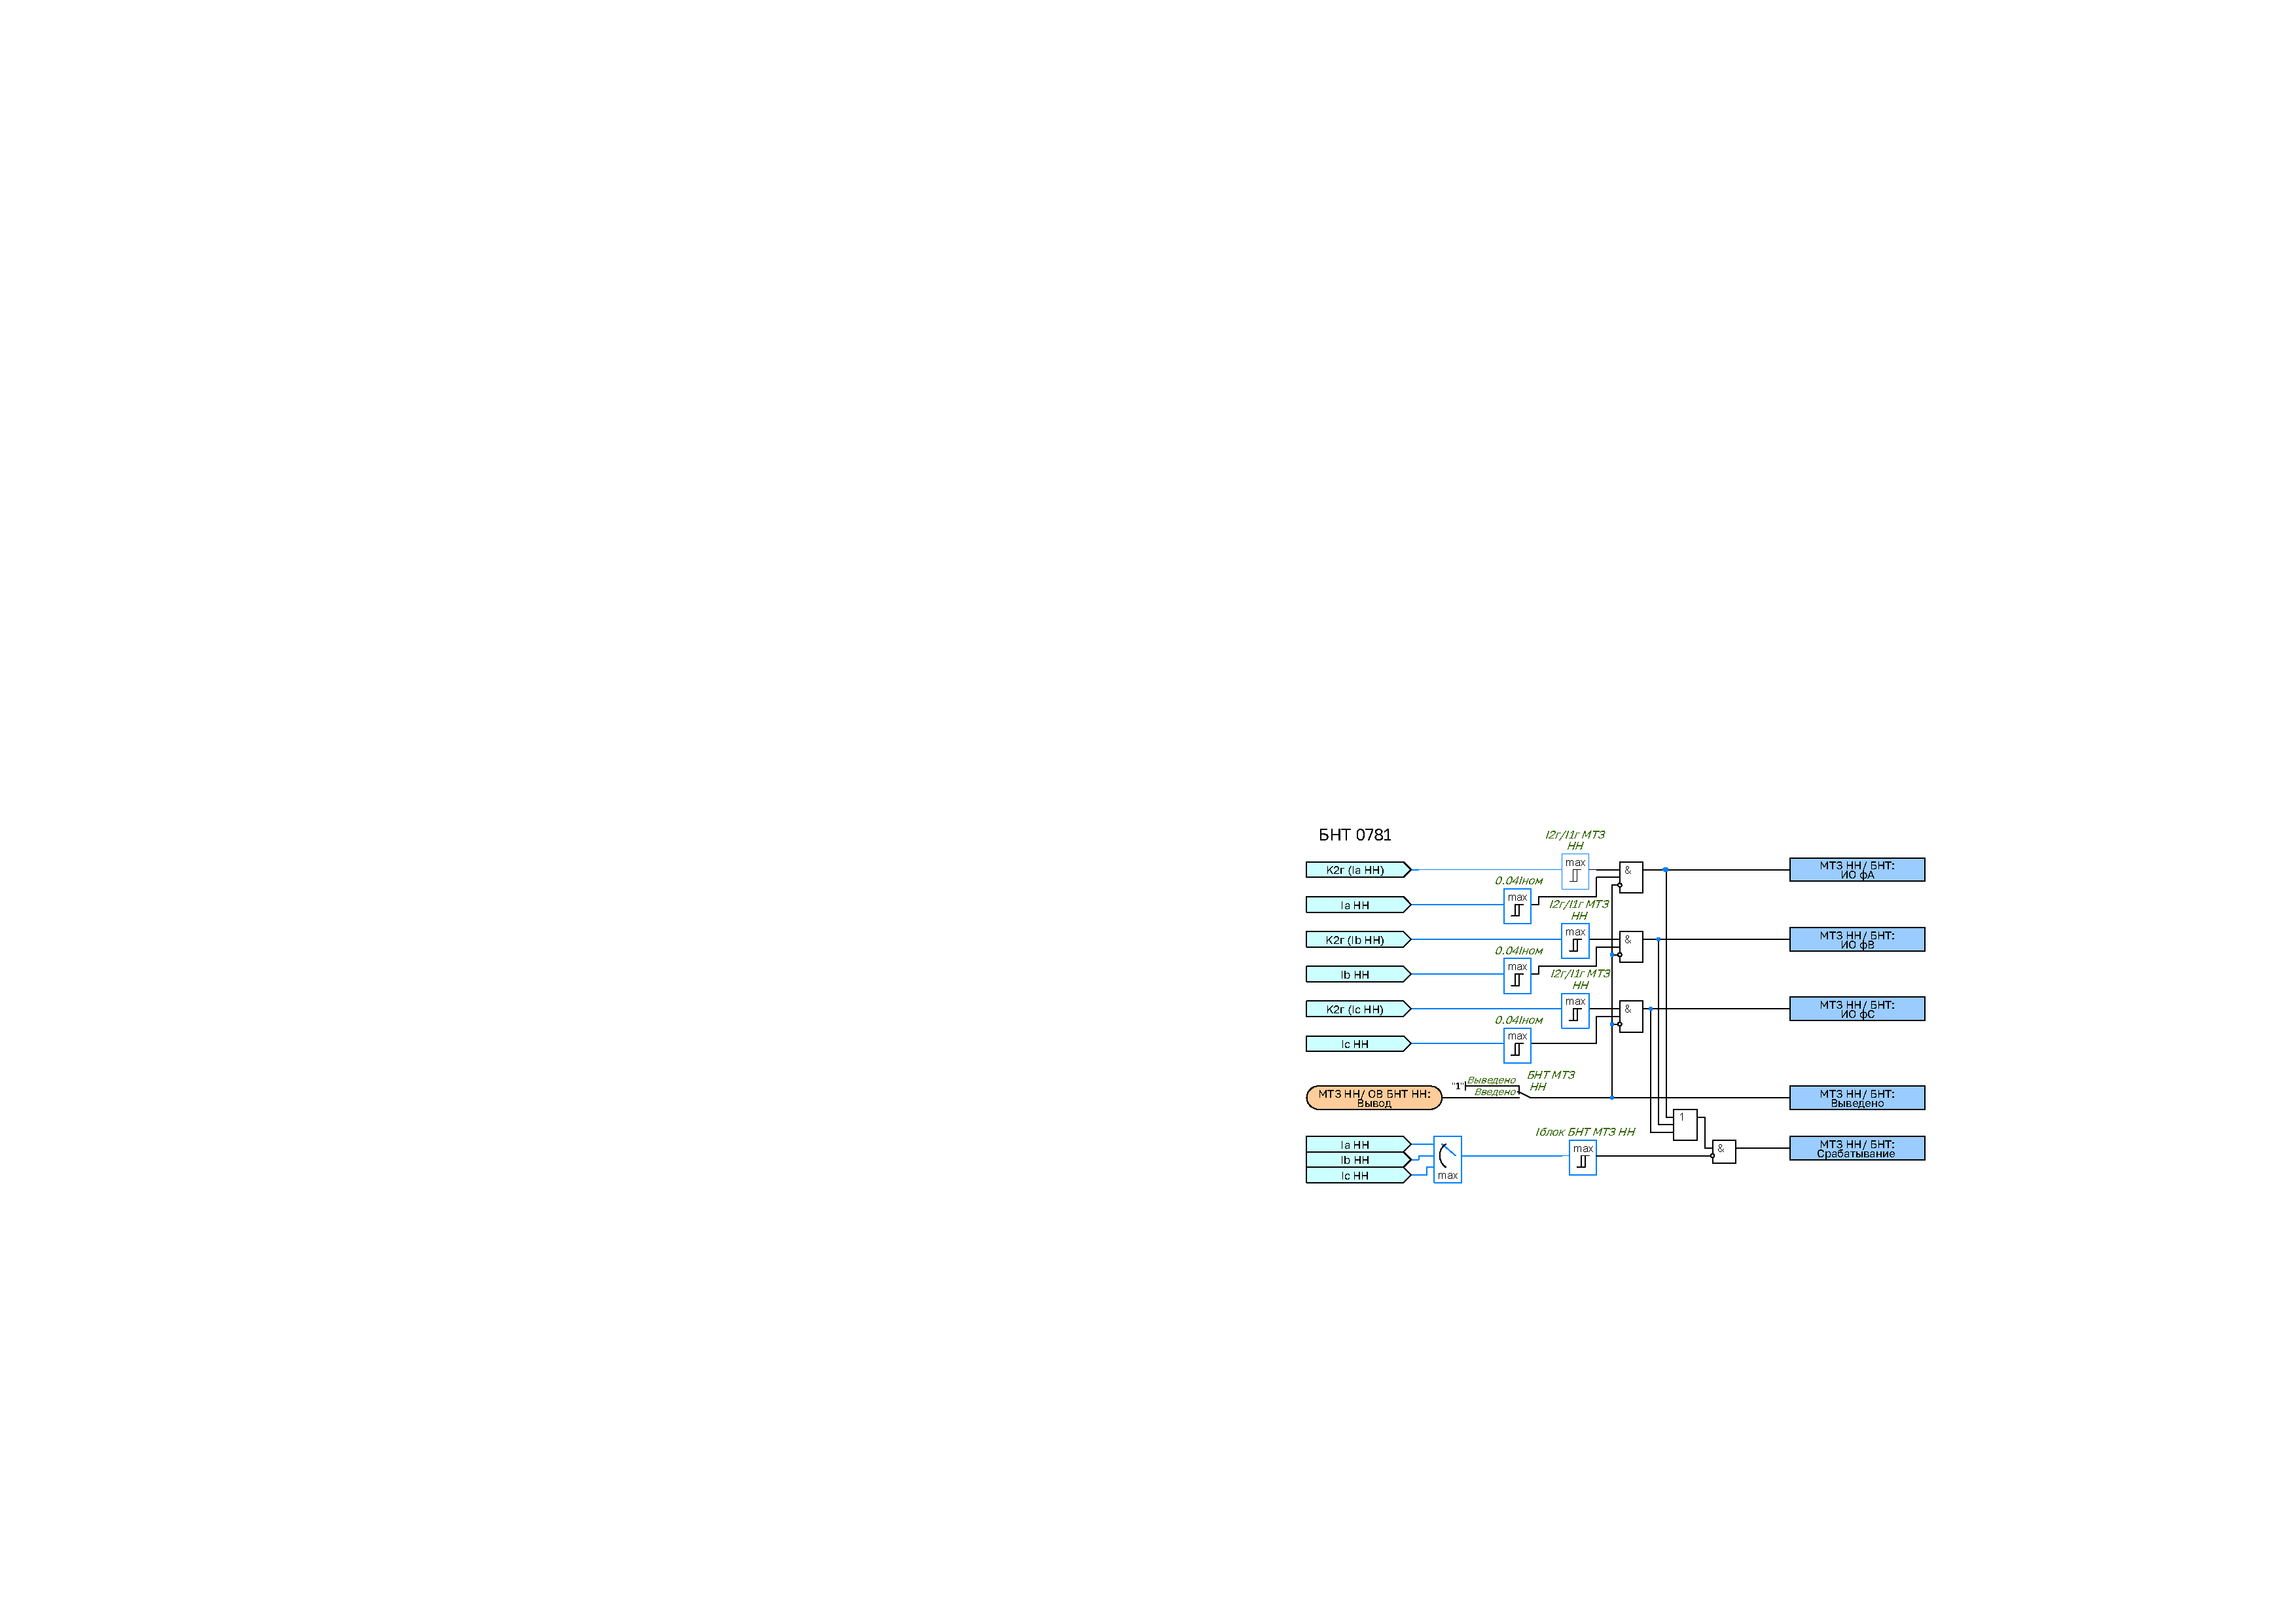
\includegraphics[width=1\textwidth,height=1\textheight,keepaspectratio]{img11.pdf}
\captionof{figure}{Функциональная схема логики органа выявления БНТ}\label{pict:mtz_bnt}
\end{figure}




\end{enumerate}
\needspace{2\baselineskip}
\color{unidarkgreen}{\subsection{Комбинированный пуск по напряжению стороны НН}}
\color{black}

\begin{enumerate}[label=\arabic{section}.\arabic{subsection}.\arabic*,  align=left, labelsep=4pt, leftmargin=0pt, itemindent=57pt]

\item
Комбинированный пусковой орган по напряжению низкой и средней сторон трансформатора используется для повышения чувствительности МТЗ НН.   

\item
Цепи напряжения подключаются к ТН, установленным на шинах низшего напряжения.

\item
Внутренний комбинированный пусковой орган напряжения (КПОН), контролирует минимальное линейное напряжение и максимальное напряжение обратной последовательности низкой стороны трансформатора. Порог срабатывания пуска по минимальному линейному напряжению задается уставками \textbf{«Uл КПОН НН»}, порог срабатывания пуска по максимальному напряжению обратной последовательности задается уставками \textbf{«U2 КПОН НН»}. 

\item
Уставки КПОН приведены в таблице \ref{app_set:kpon}.

\item
Ввод в работу КПОН осуществляется независимо для каждой стороны с помощью уставок \textbf{«КПОН НН»}. Оперативный ввод/вывод КПОН производится с помощью БУ (блоков управления функциями)
\textit{«Вывод КПОН НН»}.

\item
Выбор типа пуска по напряжению соответствующей стороны осуществляется с помощью уставок \textbf{«Тип КПОН НН»}: 
\begin{itemize}
\item \textit{«Umin, U2»} - пуск по минимальному линейному напряжению или максимальному напряжению обратной последовательности;
\item \textit{«Umin»} - пуск по минимальному линейному напряжению;
\item \textit{«Внеш»} - пуск по внешнему входному сигналу «Внеш. КПОН» соответствующей стороны.
\end{itemize}

\item
Предусмотрена возможность контроля цепей напряжения каждой стороны по внутренней логике (КЦН). При появлении неисправности в цепях напряжения ТН соответствующей стороны, действие логики КПОН задается уставками \textbf{«Неиспр ТН НН»}:
\begin{itemize}
\item \textit{«Выведено»} - неисправность в цепях ТН не вызывает изменения логики КПОН соответствующей стороны;
\item \textit{«Пуск КПОН»} - при появлении неисправности в цепях ТН, КПОН соответствующей стороны всегда разрешен;
\item \textit{«Блок КПОН»} - при появлении неисправности в цепях ТН, КПОН соответствующей стороны блокируется до исчезновения неисправности ТН.
\end{itemize}

\item
Алгоритм работы КПОН НН приведен на рисунке на рисунке \ref{pic:KPON}. Алгоритмы работы КПОН НН1, КПОН НН2 выполнены аналогично.

\begin{figure}[H]
\centering
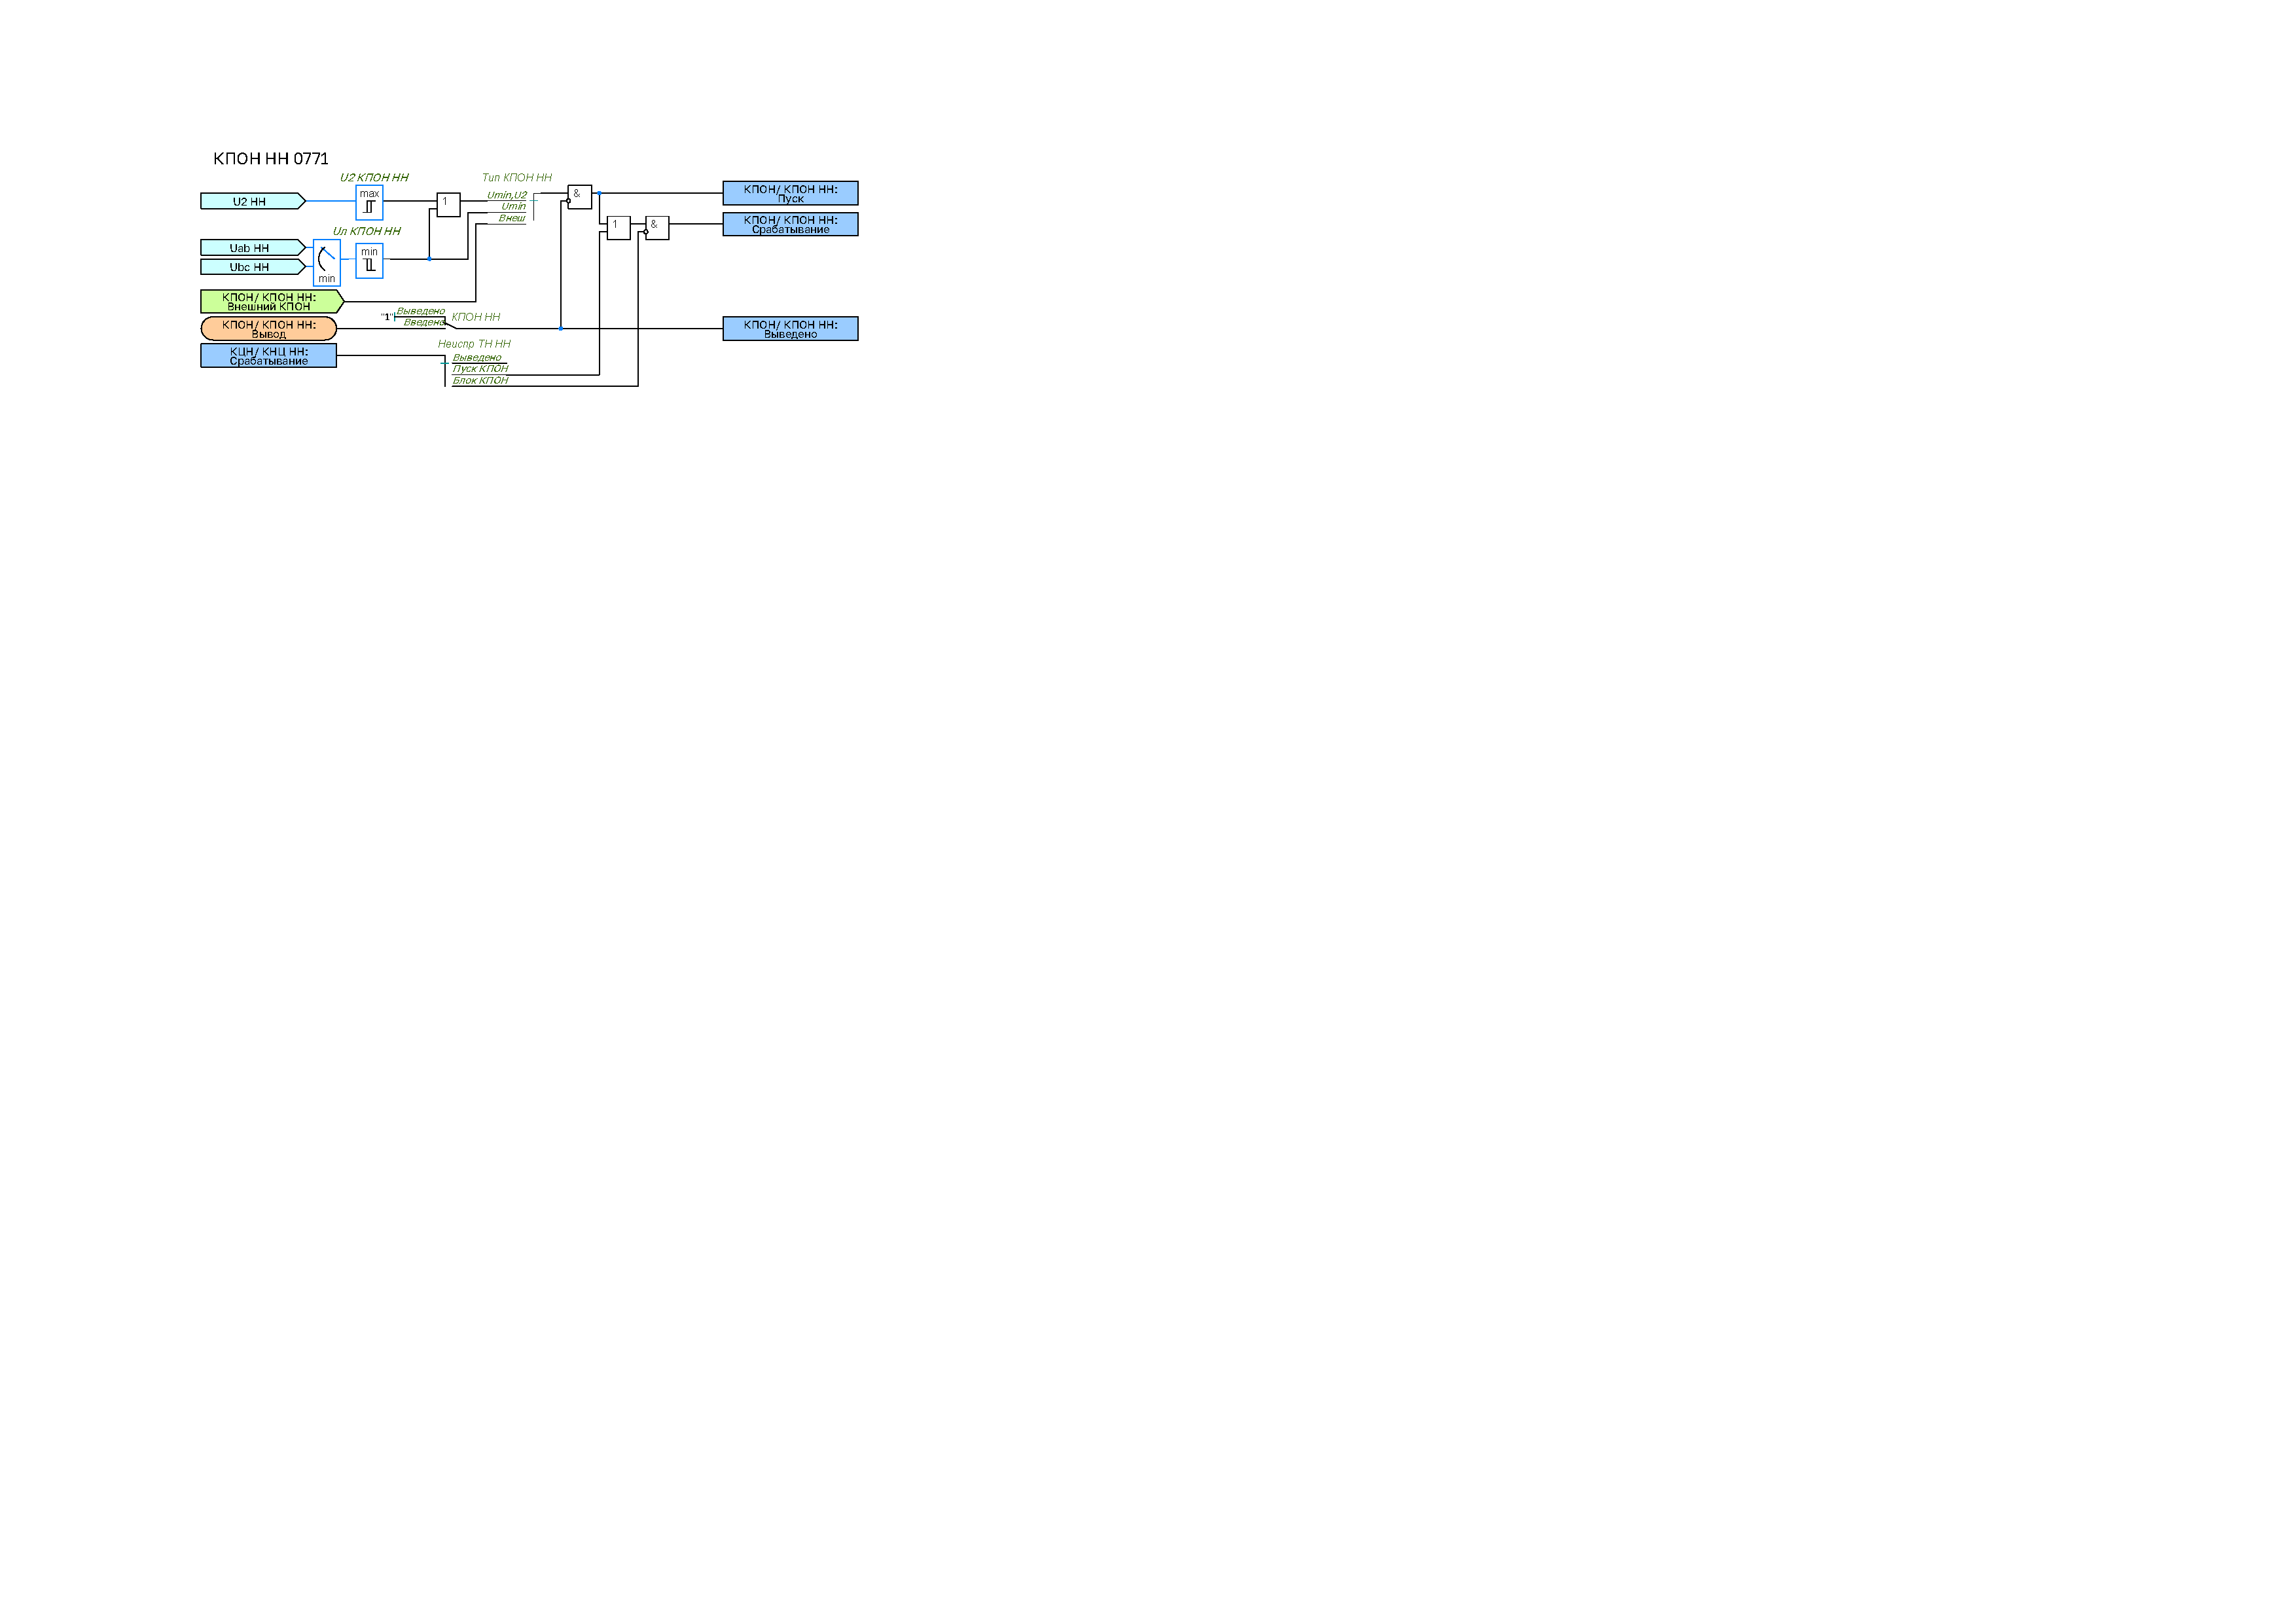
\includegraphics[width=1\textwidth,height=1\textheight,keepaspectratio]{img12.pdf}
\captionof{figure}{Функциональная схема логики КПОН НН}\label{pic:KPON}
\end{figure}


\end{enumerate}\color{unidarkgreen}{\subsection{Газовая защита}}
\color{black}

\begin{enumerate}[label=\arabic{section}.\arabic{subsection}.\arabic*,  align=left, labelsep=4pt, leftmargin=0pt, itemindent=57pt]

\item
Газовое реле трансформатора (в составе ГЗ АТ, ГЗ ЛРТ) реагирует на выделение газа при повреждениях внутри кожуха, а также на понижение уровня масла. Для защиты устройства РПН применяется струйное реле (в составе ГЗ РПН), которое реагирует на ускоренный поток масла, возникающий при повреждениях в баке РПН.

\item 
Уставки ГЗ АТ приведены в таблицах \ref{app_set:gzotkl}, \ref{app_set:gzsign}. Уставки ГЗ ЛРТ приведены в таблицах \ref{app_set:gzlrtotkl}, \ref{app_set:gzlrtsign}. Уставки ГЗ РПН приведены в таблице \ref{app_set:gzrpn}.

\item
Предусмотрена возможность приема сигналов срабатывания сигнального контакта ГЗ АТ, отключающего контакта ГЗ АТ и низкой изоляции цепи отключающего контакта ГЗ АТ, по разным цепям от двух источников ПДС1 и ПДС2. Для приема сигналов от ПДС1 предусмотрены входные сигналы \textit{«Ср.сигн контакта ГЗ АТ 1 цепь»}, \textit{«Ср. откл контакта ГЗ АТ 1 цепь»} и \textit{«Низкая изол. ГЗ АТ откл 1 цепь»}, а для приема сигналов от ПДС2 предусмотрены входные сигналы \textit{«Ср. сигн контакта ГЗ АТ 2 цепь»}, \textit{«Ср. откл контакта ГЗ АТ 2 цепь»} и \textit{«Низкая изол. ГЗ АТ откл 2 цепь»}. Если сигналы срабатывания ГЗ АТ заводятся непосредственно со шкафа ШОМ силового трансформатора, то конфигурируются только входные сигналы \textit{«Ср. сигн контакта ГЗ АТ 1 цепь»}, \textit{«Ср. откл контакта ГЗ АТ 1 цепь»} и \textit{«Низкая изол. ГЗ АТ откл 1 цепь»}, а действие ГЗ АТ по второй цепи сигнального и отключающего контакта выводится из работы с помощью уставок \textbf{«ГЗ АТ сигн 2 цепь»} и \textbf{«ГЗ АТ откл 2 цепь»}.

\item
Ввод в работу ГЗ АТ осуществляется с помощью уставок \textbf{«ГЗ АТ сигн 1 цепь»}, \textbf{«ГЗ АТ сигн 2 цепь»}, \textbf{«ГЗ АТ откл 1 цепь»} и \textbf{«ГЗ АТ откл 2 цепь»}. Оперативный перевод ГЗ АТ на сигнал производится с помощью команд управления \textit{«Перевод ГЗ АТ откл на сигнал»}. Предусматривается возможность действия срабатывания сигнального контакта ГЗ АТ на отключение трансформатора с помощью уставки
\textbf{«Откл АТ от ГЗ сигн»}.

\item
Оперативный ввод/вывод сигнальной ступени ГЗ АТ производится с помощью БУ (блока управления функциями) \textit{«Вывод ГЗ АТ сигн»}, а оперативный ввод/вывод отключающей ступени ГЗ АТ  производится с помощью БУ (блока управления функциями) \textit{«Вывод ГЗ АТ откл»}.

\item
Непрерывный контроль изоляции цепи отключающего контакта ГЗ АТ осуществляется с помощью реле контроля изоляции (РКИ). В случае снижения сопротивления изоляции РКИ подает сигнал \textit{«Низкая изол. ГЗ АТ откл 1 цепь»} (\textit{«Низкая изол. ГЗ АТ откл 2 цепь»}) для блокировки действия ГЗ АТ по цепи отключающего контакта. Время срабатывания блокировки от сигналов РКИ задается с помощью уставки \textbf{«Тбл ГЗ АТ откл»}. Ввод блокировки ГЗ АТ от РКИ осуществляется с помощью уставки \textbf{«Блок ГЗ АТ откл»}. Для сброса блокировки от РКИ, используется команда управления \textit{«Возврат ГЗ АТ откл»}.

\item
Алгоритм работы сигнальной ступени ГЗ АТ приведен на рисунке \ref{pic:GZAT_sign}, алгоритм работы отключающей ступени ГЗ АТ приведен на рисунке \ref{pic:GZAT_otkl}. Алгоритмы работы сигнальной и отключающей ступеней ГЗ ЛРТ выполнены аналогично соответствующим ступеням ГЗ АТ.

\begin{figure}[H]
\centering
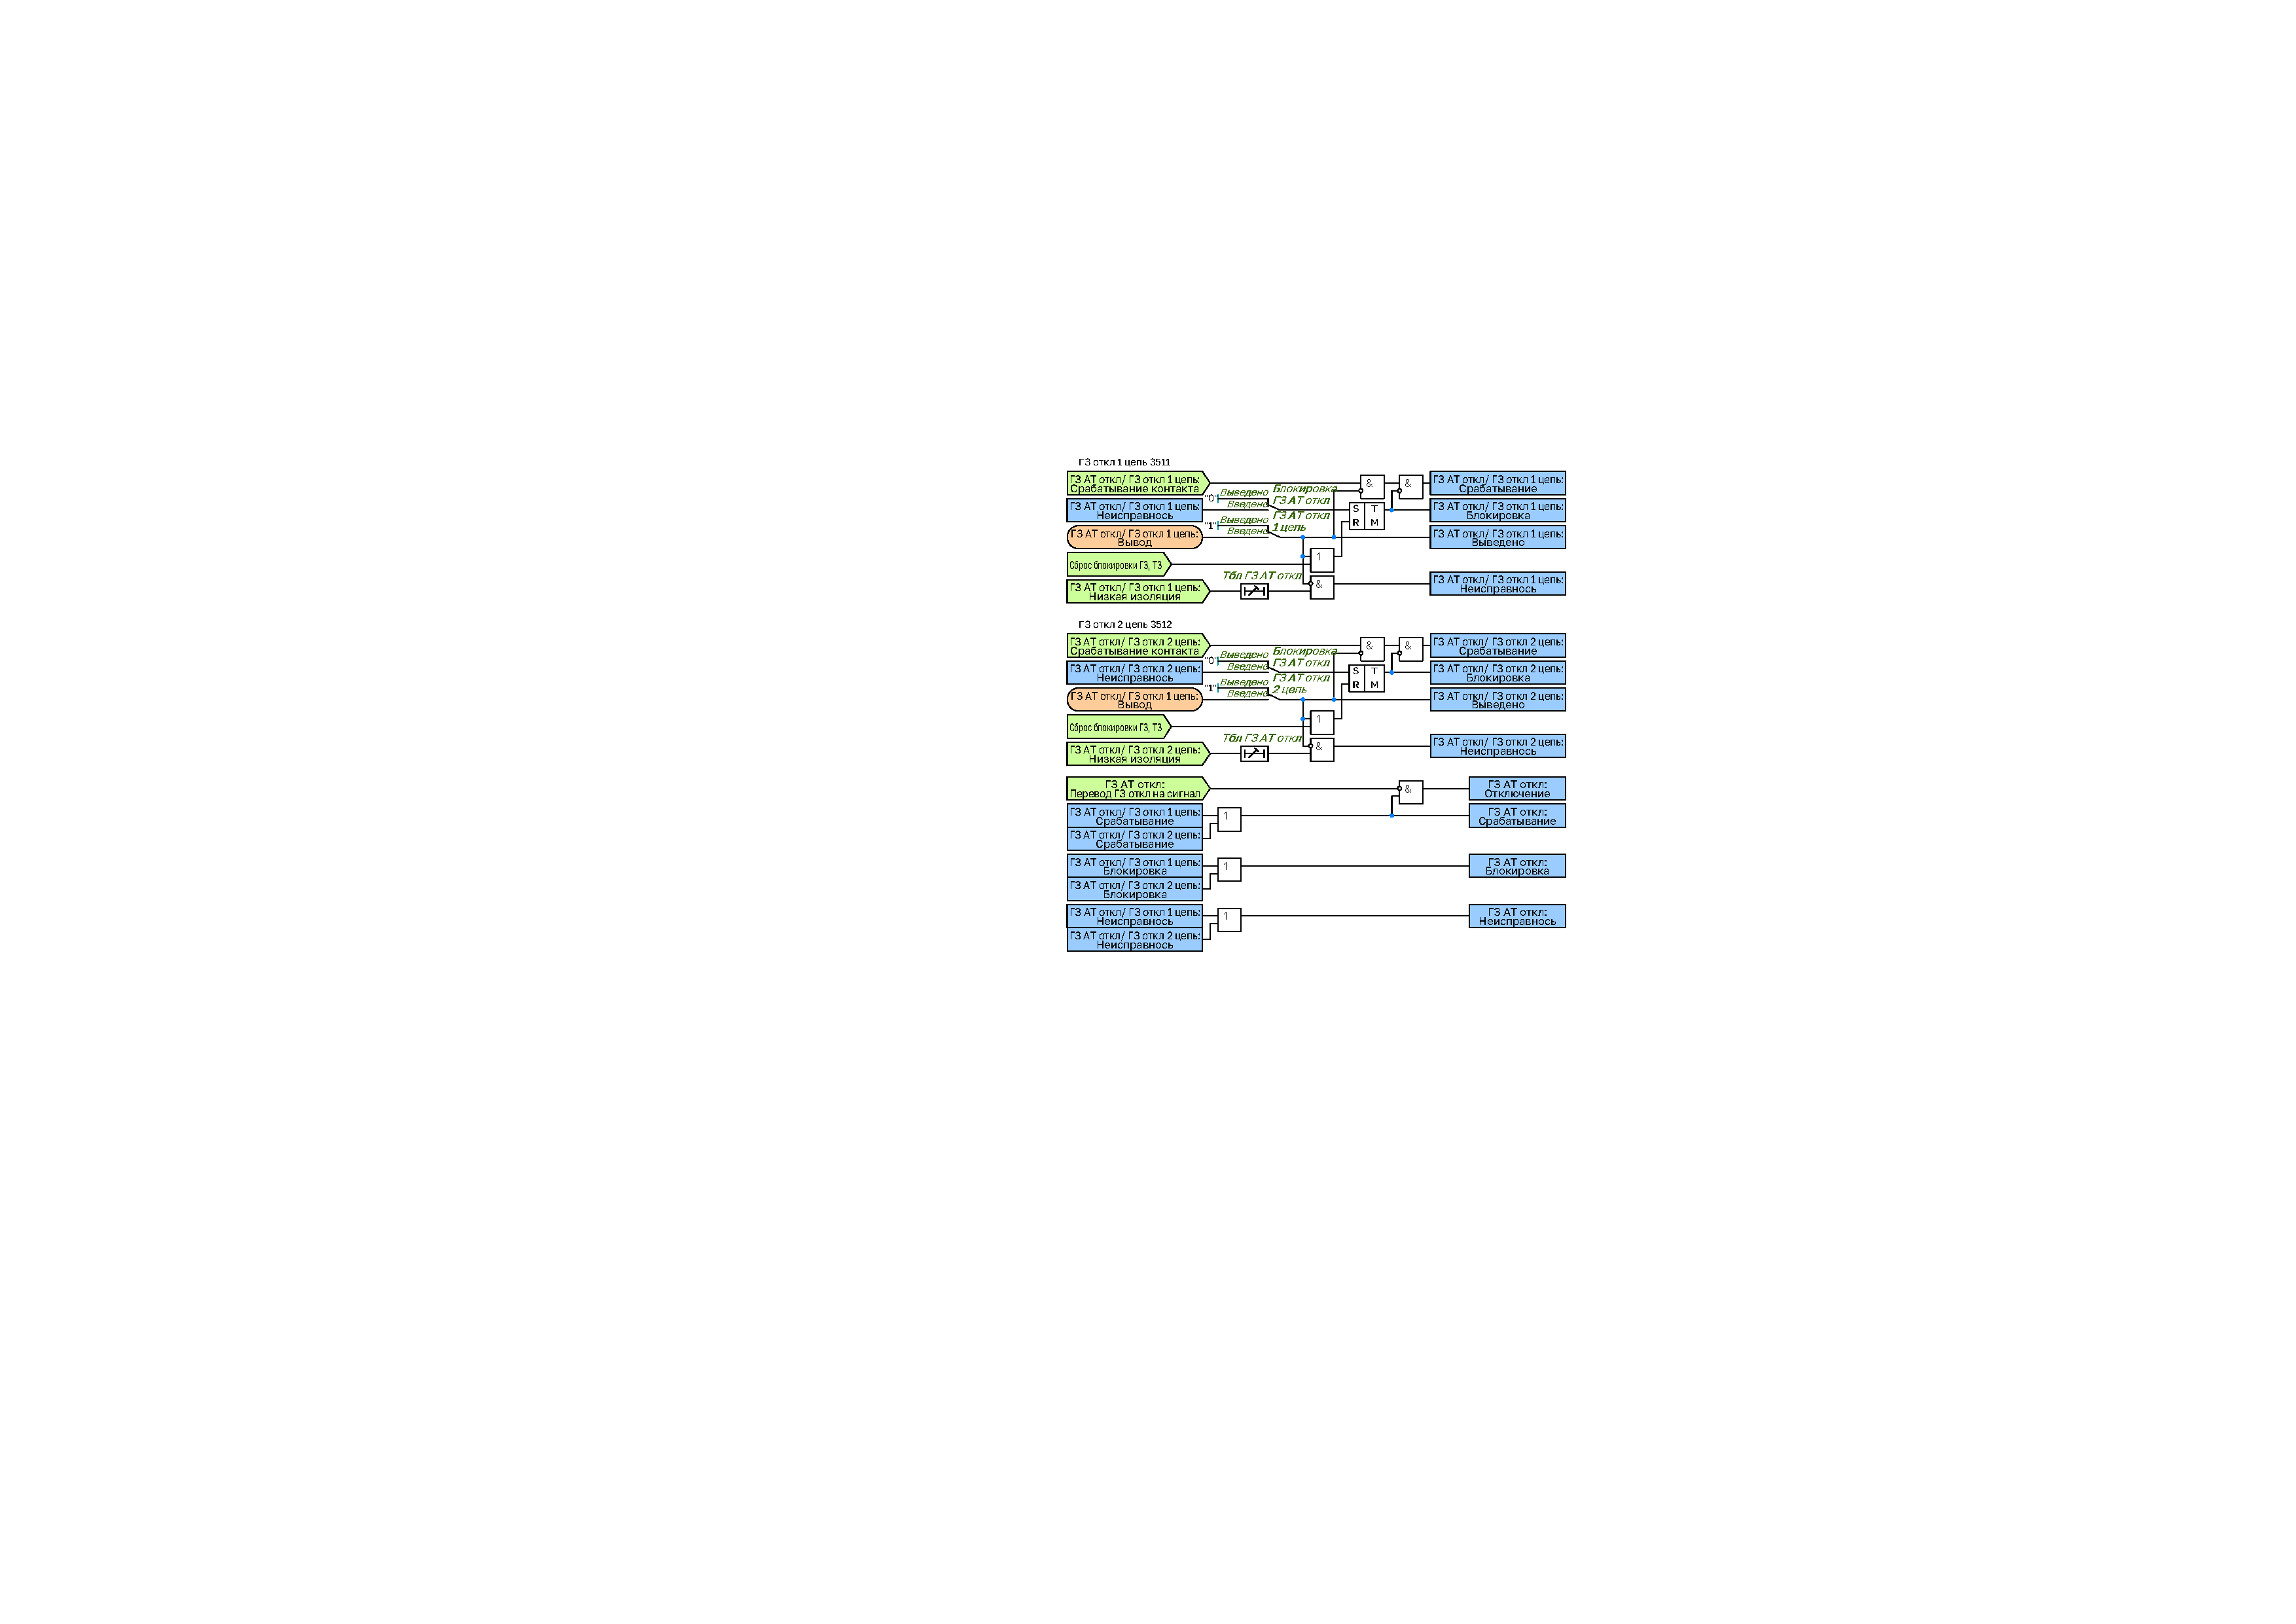
\includegraphics[width=0.6\textwidth,height=0.6\textheight,keepaspectratio]{img13.pdf}
\captionof{figure}{Функциональная схема логики отключающей ступени ГЗ АТ}\label{pic:GZAT_otkl}
\end{figure}

\vspace{2mm}
\begin{figure}[H]
\centering
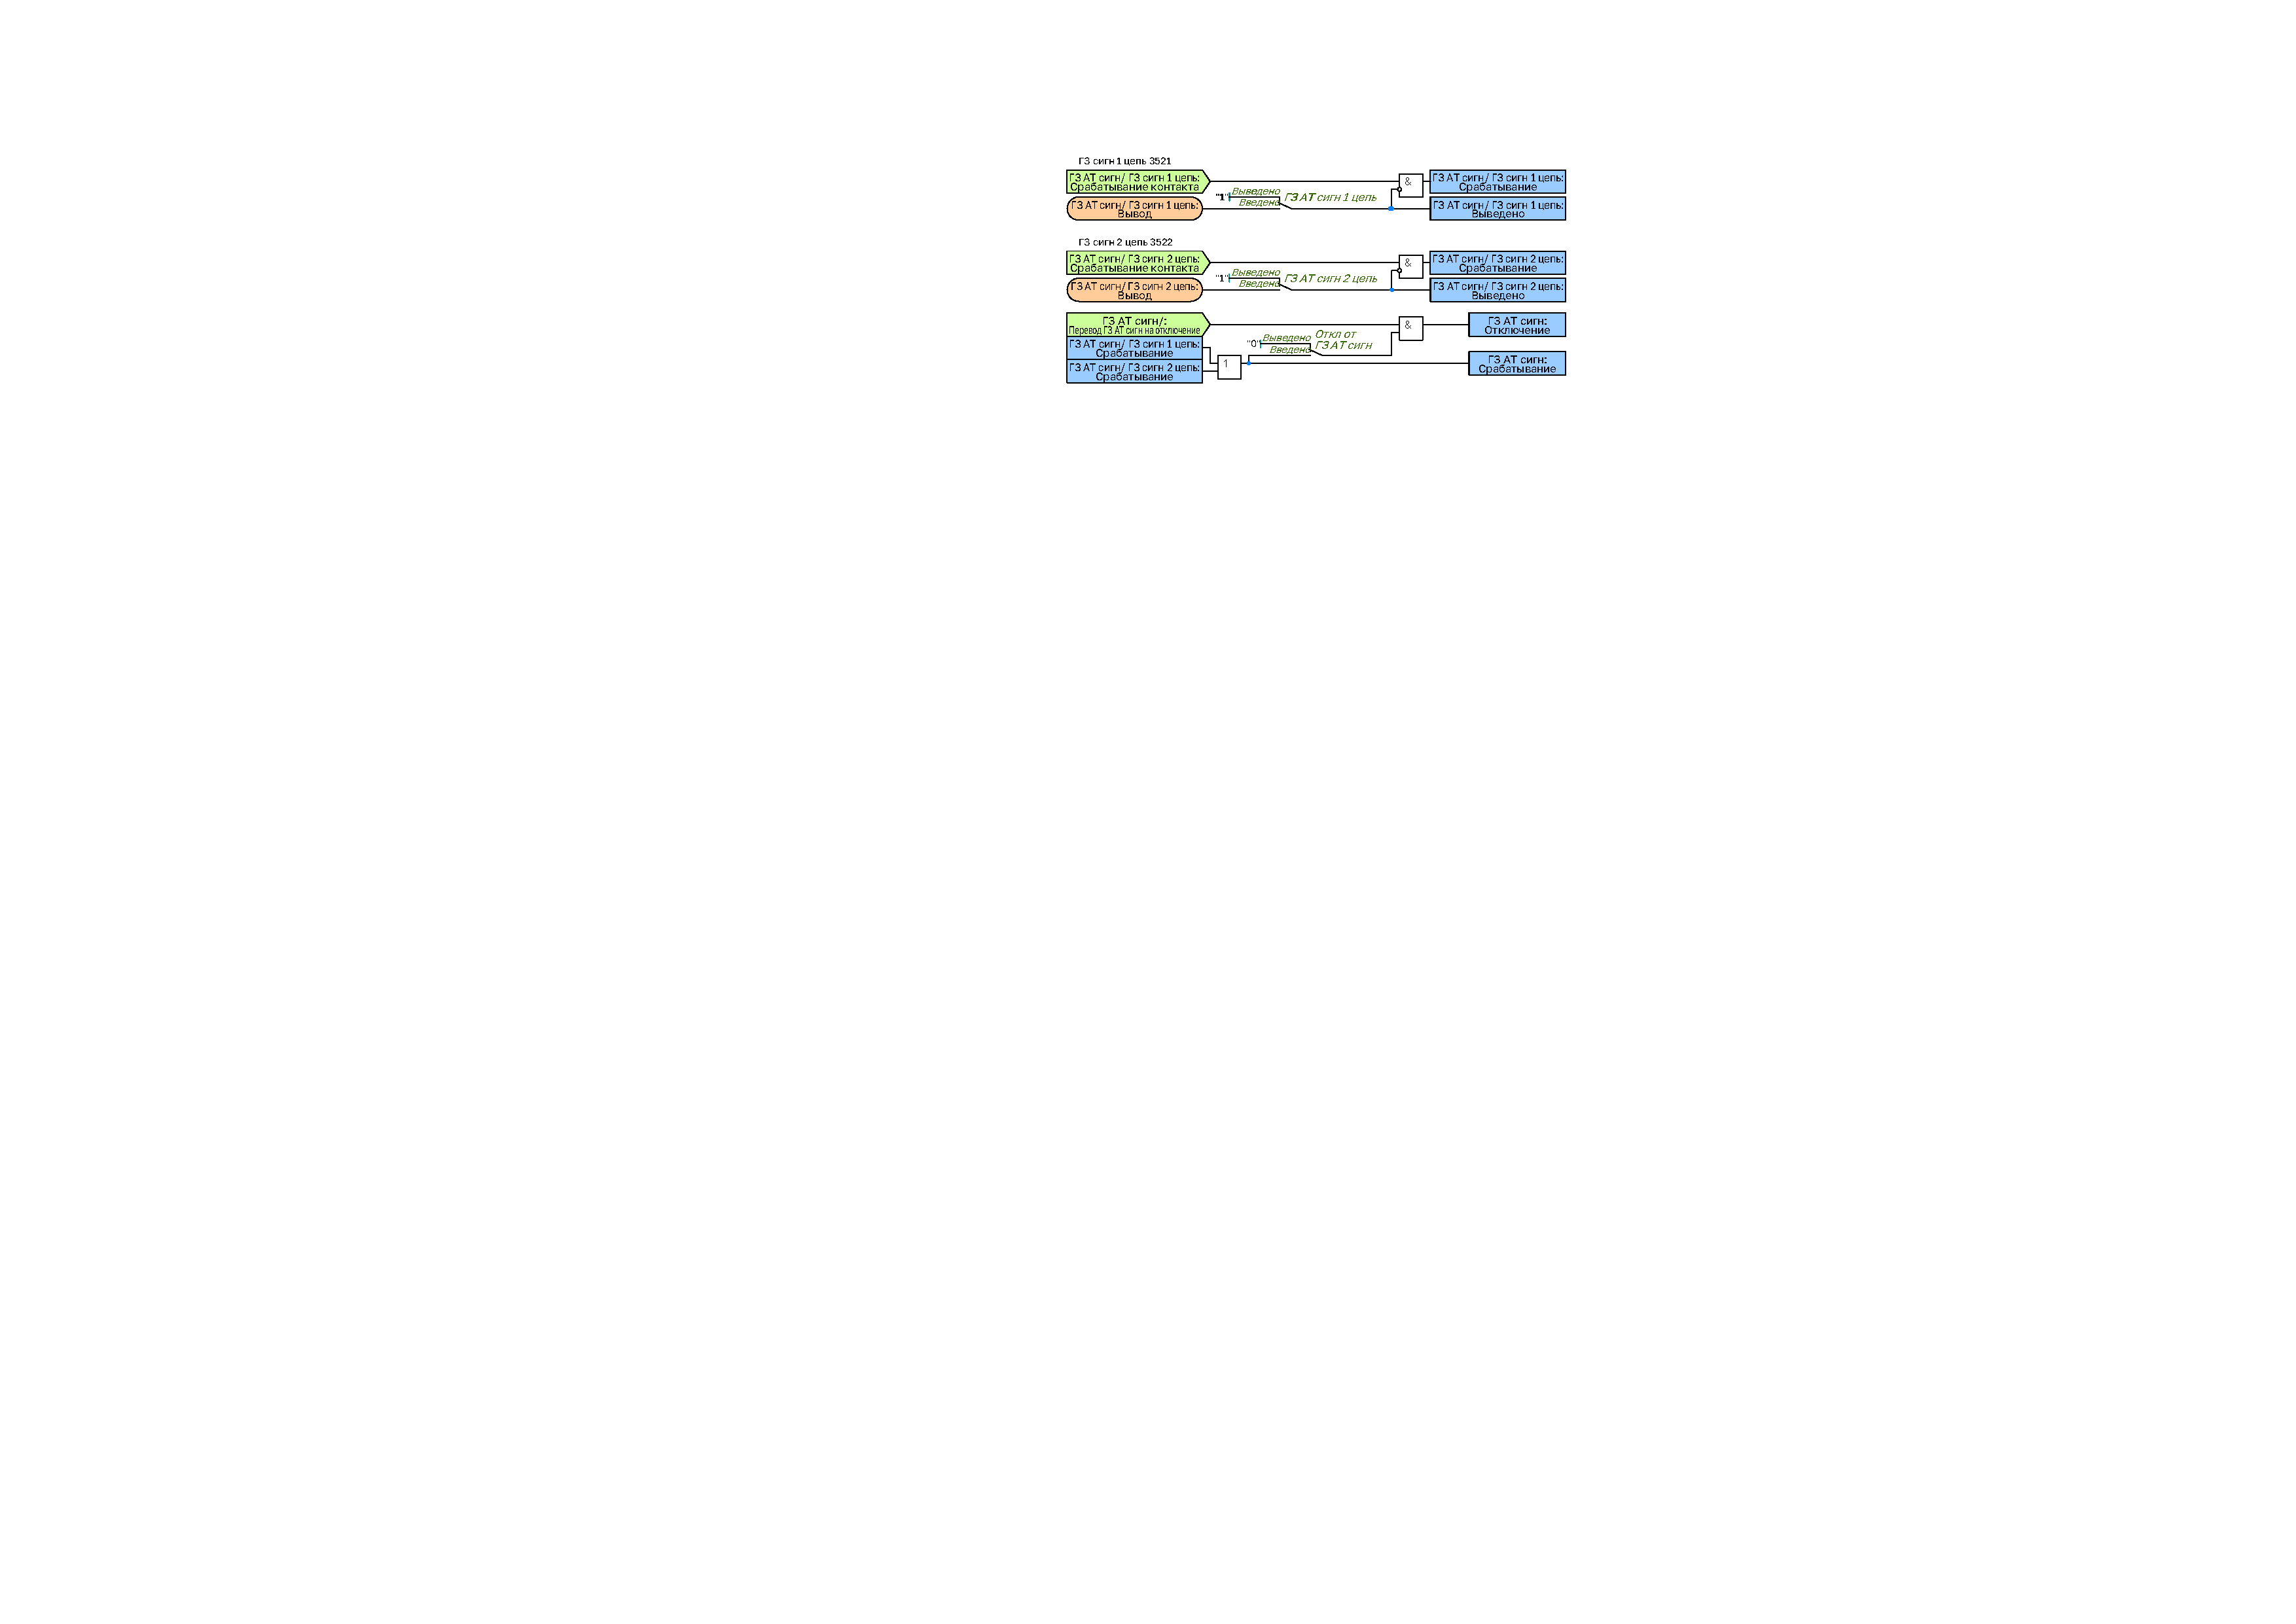
\includegraphics[width=0.65\textwidth,height=0.65\textheight,keepaspectratio]{img14.pdf}
\captionof{figure}{Функциональная схема логики сигнальной ступени ГЗ АТ}\label{pic:GZAT_sign}
\end{figure}

\item
Алгоритм работы ГЗ РПН приведен на рисунке \ref{pic:GZRPN}.
\vspace{2mm}
\begin{figure}[H]
\centering
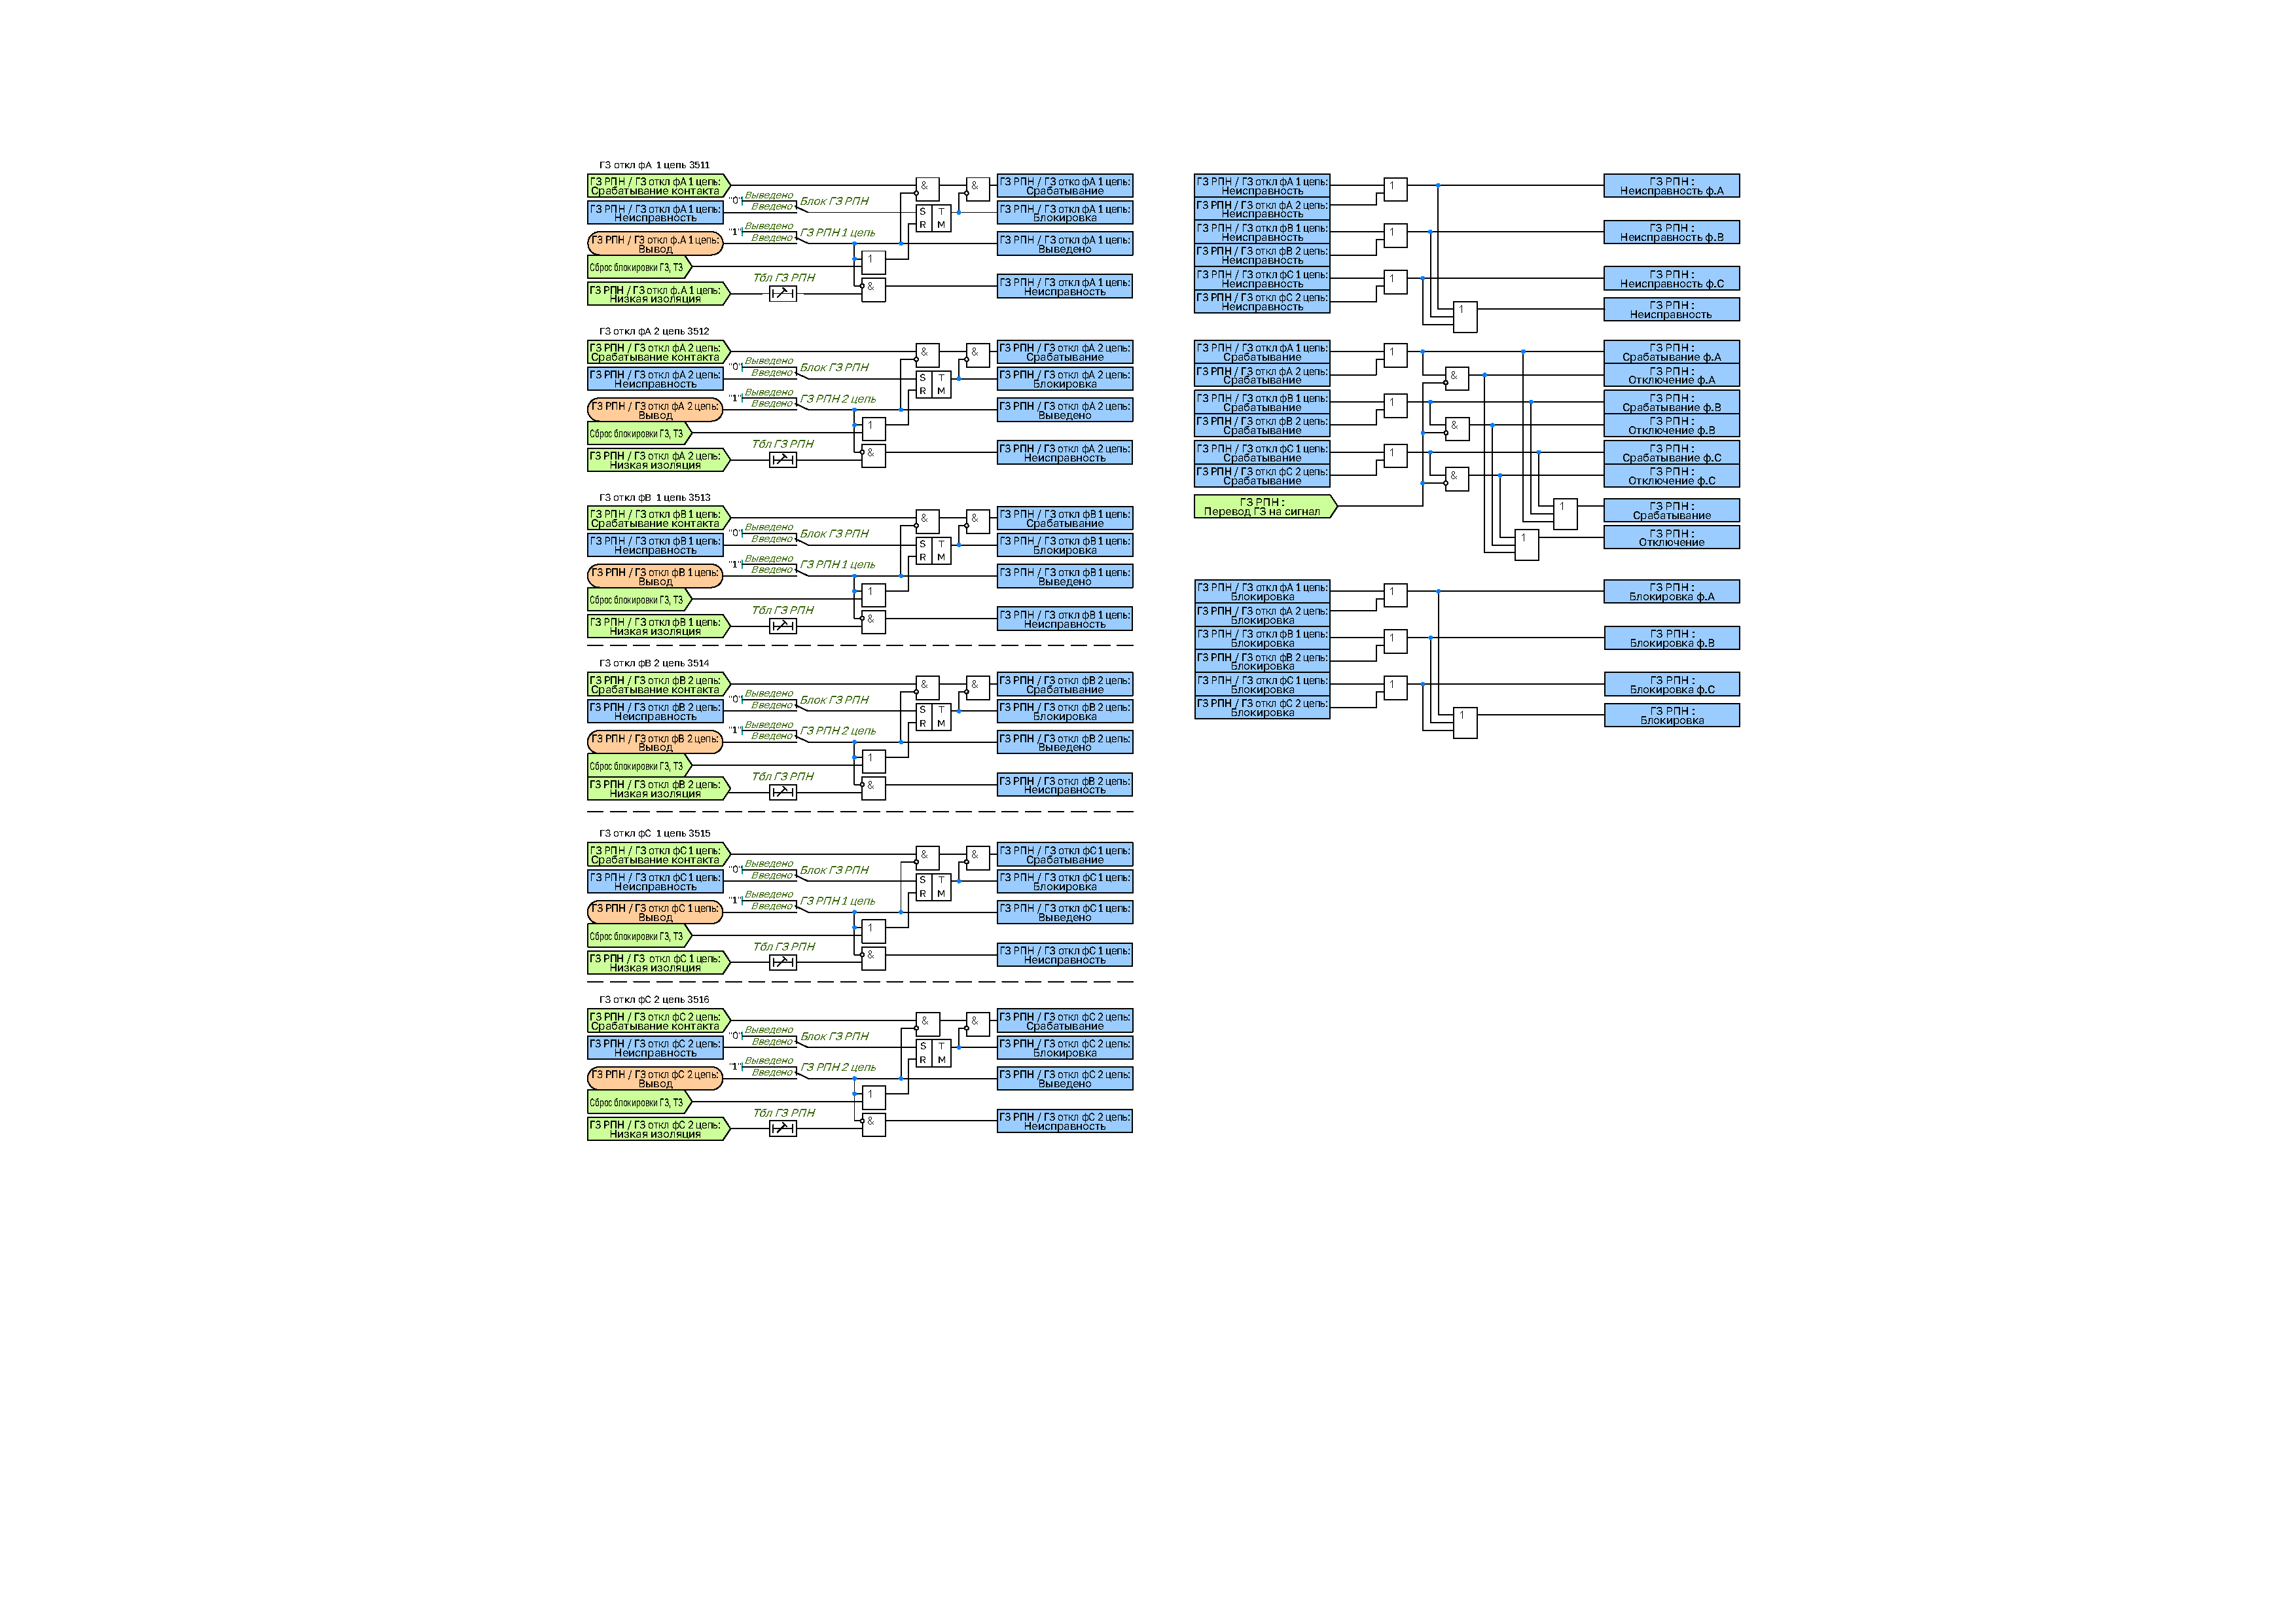
\includegraphics[width=1\textwidth,height=1\textheight,keepaspectratio]{img15.pdf}
\captionof{figure}{Функциональная схема логики ГЗ РПН}\label{pic:GZRPN}
\end{figure}






\end{enumerate}\color{unidarkgreen}{\subsection{Технологические защиты}}
\color{black}

\begin{enumerate}[label=\arabic{section}.\arabic{subsection}.\arabic*,  align=left, labelsep=4pt, leftmargin=0pt, itemindent=57pt]

\item
Технологические защиты от повышения давления, температуры масла и обмоток предназначены для предотвращения повреждения трансформаторного оборудования при нарушениях режима работы. Для автотрансформатора и ЛРТ предусматриваются функциональные блоки приема и обработки сигналов от датчиков температуры масла и обмоток; для ЛРТ также предусматривается прием сигналов от реле давления.

\item
Предусмотрена возможность приема сигналов срабатывания сигнального и аварийного контактов датчиков температуры масла и обмотки автотрансформатора (ДТм АТ и ДТо АТ), а также сигналов низкой изоляции цепей аварийных контактов, по двум независимым цепям от источников ПДС1 и ПДС2. Для приема сигналов от ПДС1 предусмотрены входные сигналы \textit{«Ср. сигн контакта ДТм (ДТо) АТ 1 цепь»}, \textit{«Ср. авар контакта ДТм (ДТо) АТ 1 цепь»} и \textit{«Низкая изол. ДТм (ДТо) АТ авар 1 цепь»}; для ПДС2 — соответственно \textit{«... 2 цепь»}. Если сигналы заводятся непосредственно со шкафа ШОМ, конфигурируются только сигналы по первой цепи, а действие по второй цепи сигнального и аварийного контактов выводится уставками \textbf{«ДТм (ДТо) АТ сигн 2 цепь»} и \textbf{«ДТм (ДТо) АТ авар 2 цепь»}

\item
Ввод в работу ДТм АТ (ДТо АТ) осуществляется с помощью уставок \textbf{«ДТм АТ (ДТо АТ) сигн 1 цепь»}, \textbf{«ДТм АТ (ДТо АТ) сигн 2 цепь»}, \textbf{«ДТм АТ  (ДТо АТ) авар 1 цепь»} и \textbf{«ДТм АТ (ДТо АТ) авар 2 цепь»}. Предусмотрена возможность действия срабатывания аварийного контакта ДТм АТ (ДТо АТ) на отключение трансформатора с помощью уставки \textbf{«Откл от ДТм АТ (ДТо АТ) авар»}.

\item
Оперативный ввод/вывод ТЗ производится с помощью БУ (блока управления функциями) \textit{«Вывод ТЗ АТ»}.

\item
Непрерывный контроль изоляции цепи аварийного контакта ДТм (ДТо) осуществляется с помощью реле контроля изоляции (РКИ). В случае снижения сопротивления изоляции РКИ подает сигнал \textit{«Низкая изол. ДТм АТ (ДТо АТ) авар 1 цепь»} (\textit{«Низкая изол. ДТм АТ (ДТо АТ) авар 2 цепь»}) для блокировки срабатывания ДТм АТ (ДТо АТ) от аварийного контакта. Время срабатывания блокировки от сигналов РКИ задается с помощью уставки \textbf{«Тбл ТЗ АТ»}. Ввод блокировки ДТм АТ (ДТо АТ) от РКИ осуществляется с помощью уставки \textbf{«Блок ТЗ АТ»}. Для сброса блокировки от РКИ, используется команда управления \textit{«Возврат ТЗ АТ»}.

\item
Алгоритм работы функций в составе ТЗ АТ приведен на рисунке \ref{pic:TZAT}, алгоритм работы ТЗ ЛРТ выполнен аналогично. Уставки ТЗ АТ приведены в таблице \ref{app_set:tzat}, уставки ТЗ ЛРТ приведены в таблице \ref{app_set:tzlrt}.

\vspace{2mm}
\begin{figure}[H]
\centering
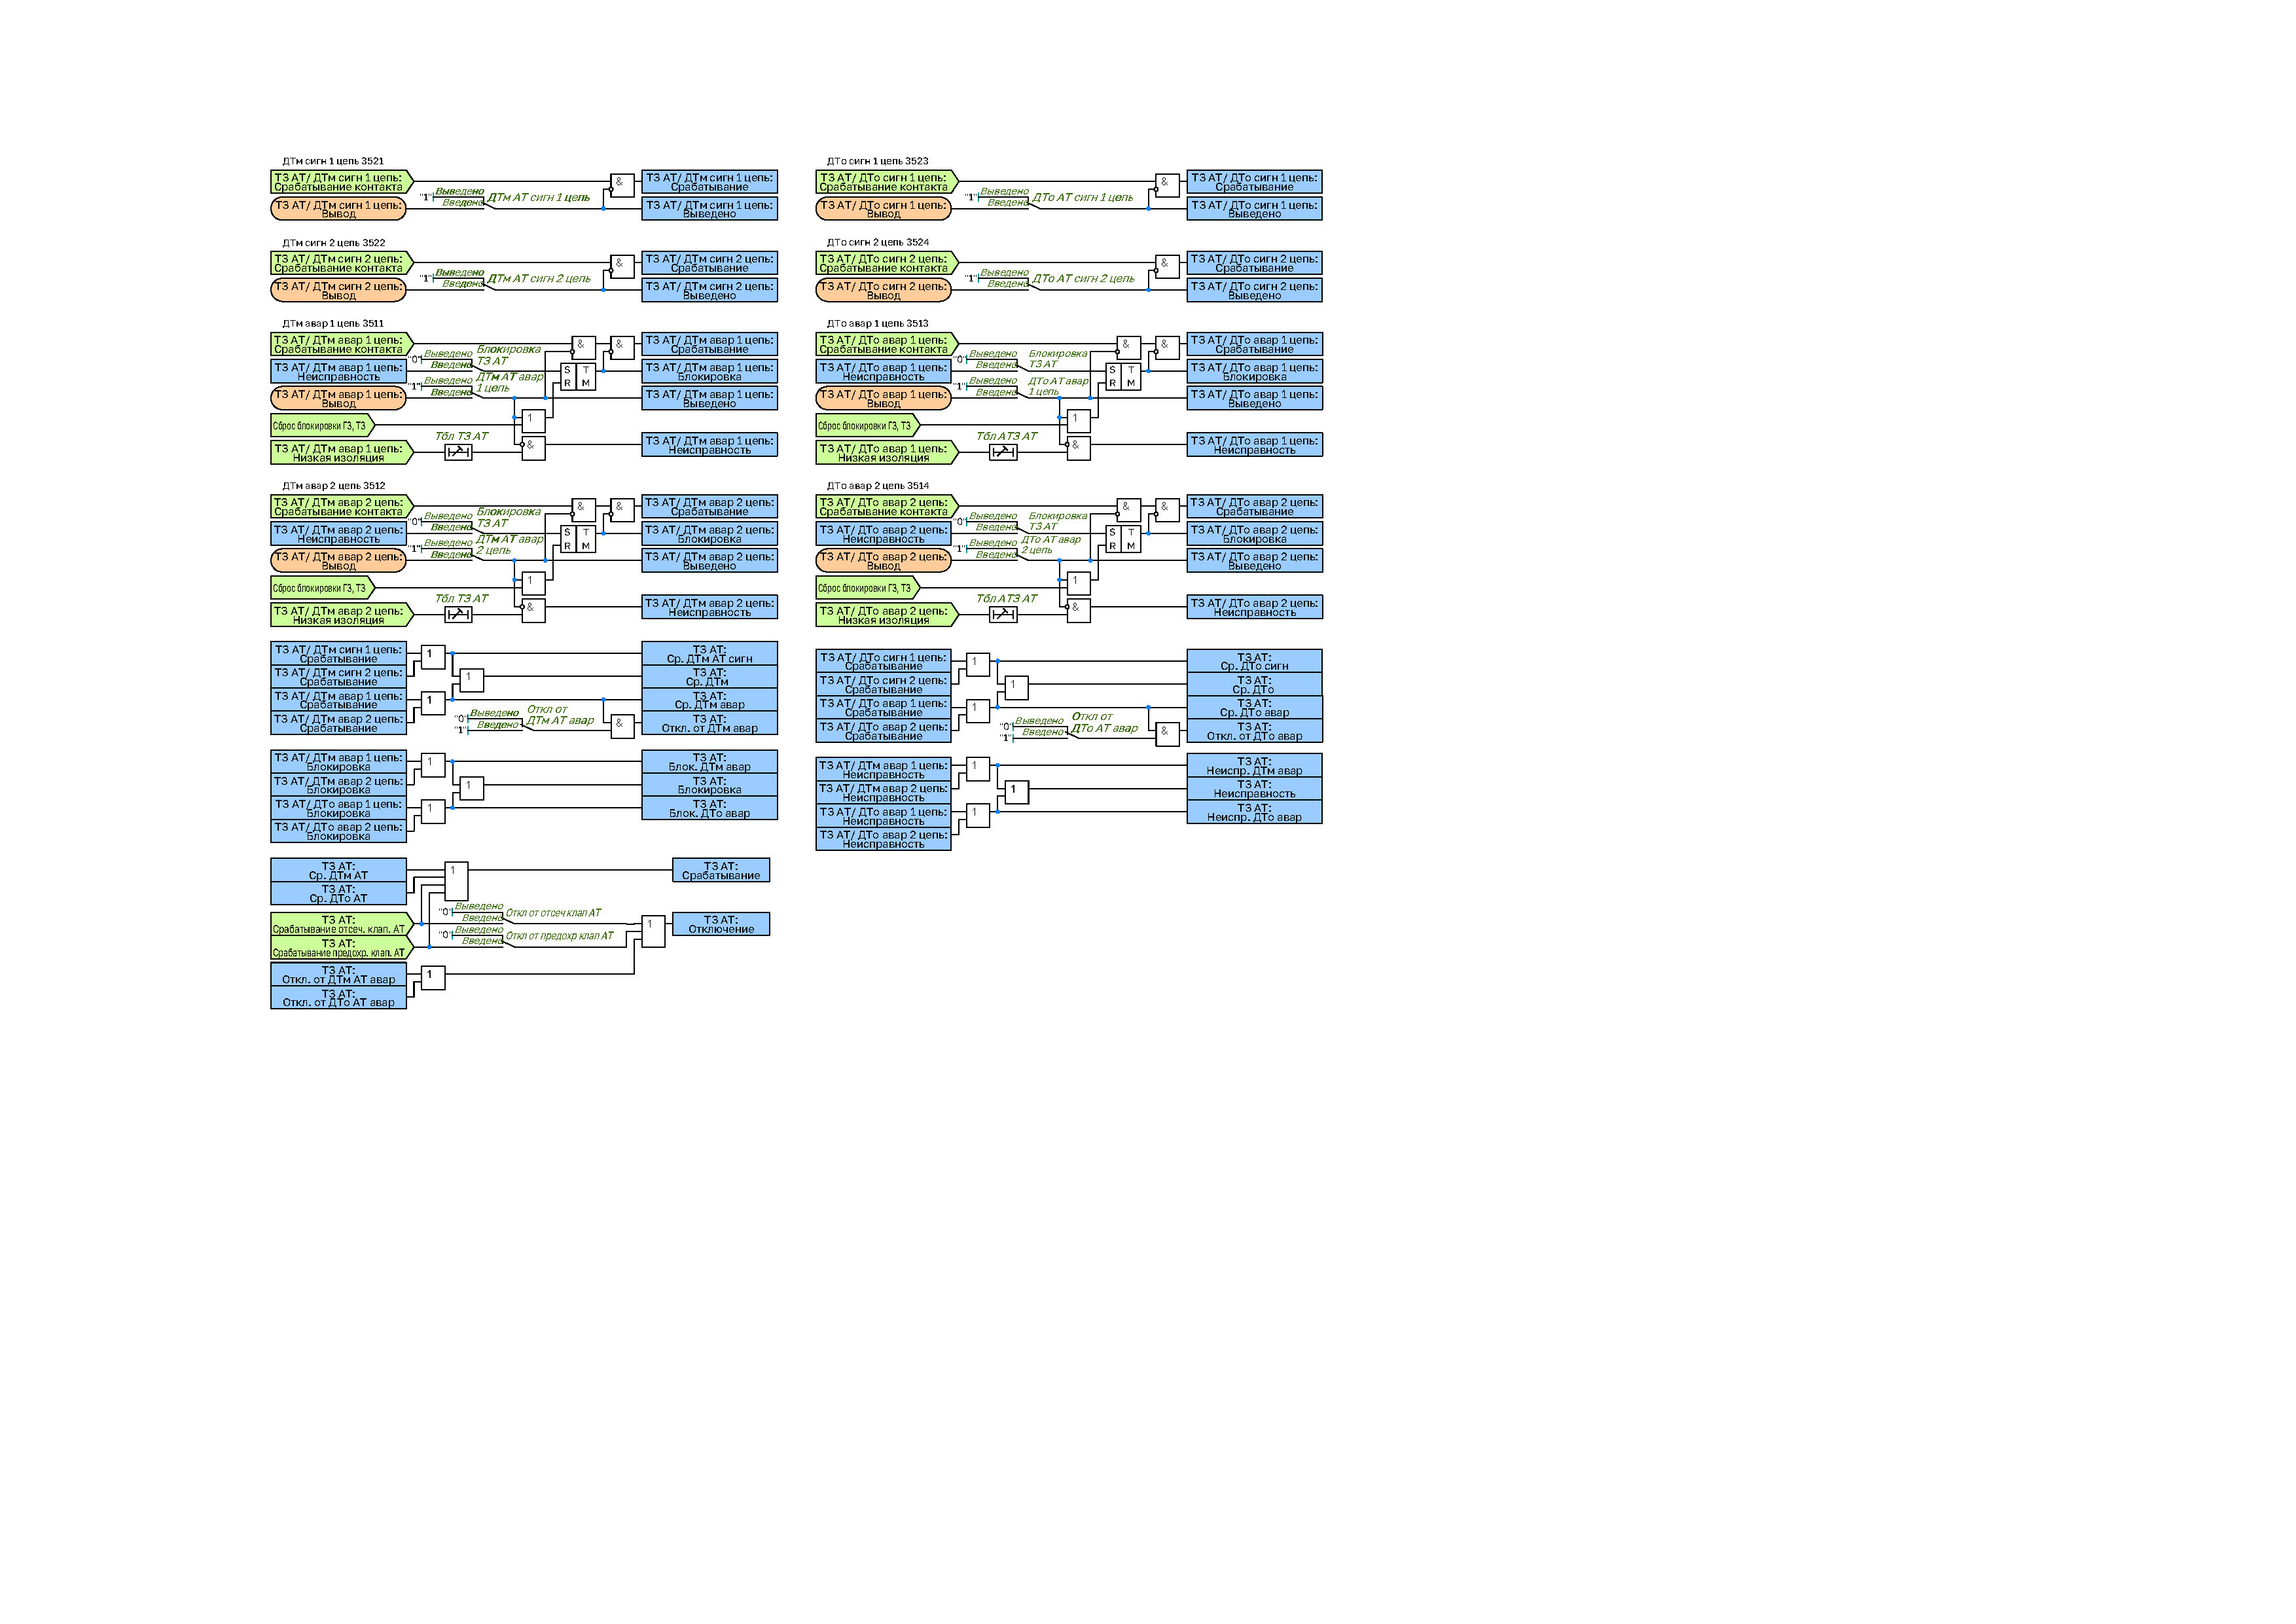
\includegraphics[width=1\textwidth,height=1\textheight,keepaspectratio]{img16.pdf}
\captionof{figure}{Функциональный блок ТЗ АТ}\label{pic:TZAT}
\end{figure}


\end{enumerate}\color{unidarkgreen}{\subsection{Токовый контроль защиты от дуговых замыканий}}
\color{black}

\begin{enumerate}[label=\arabic{section}.\arabic{subsection}.\arabic*,  align=left, labelsep=4pt, leftmargin=0pt, itemindent=57pt]

\item
Для исключения ложного срабатывания устройства дуговой защиты, которое может возникнуть при неисправности ее датчиков, предусмотрен контроль по току. Обеспечивается контроль тока трех фаз сторон ВН, СН, НН. Пороги по току срабатывания индивидуальны для каждой из контролируемых цепей.

\item
Алгоритм работы ТК ЗДЗ приведен на рисунке \ref{pic:ZDZ}. Уставки ТК ЗДЗ приведены в таблице \ref{app_set:tkzdz}.

\vspace{2mm}
\begin{figure}[H]
\centering
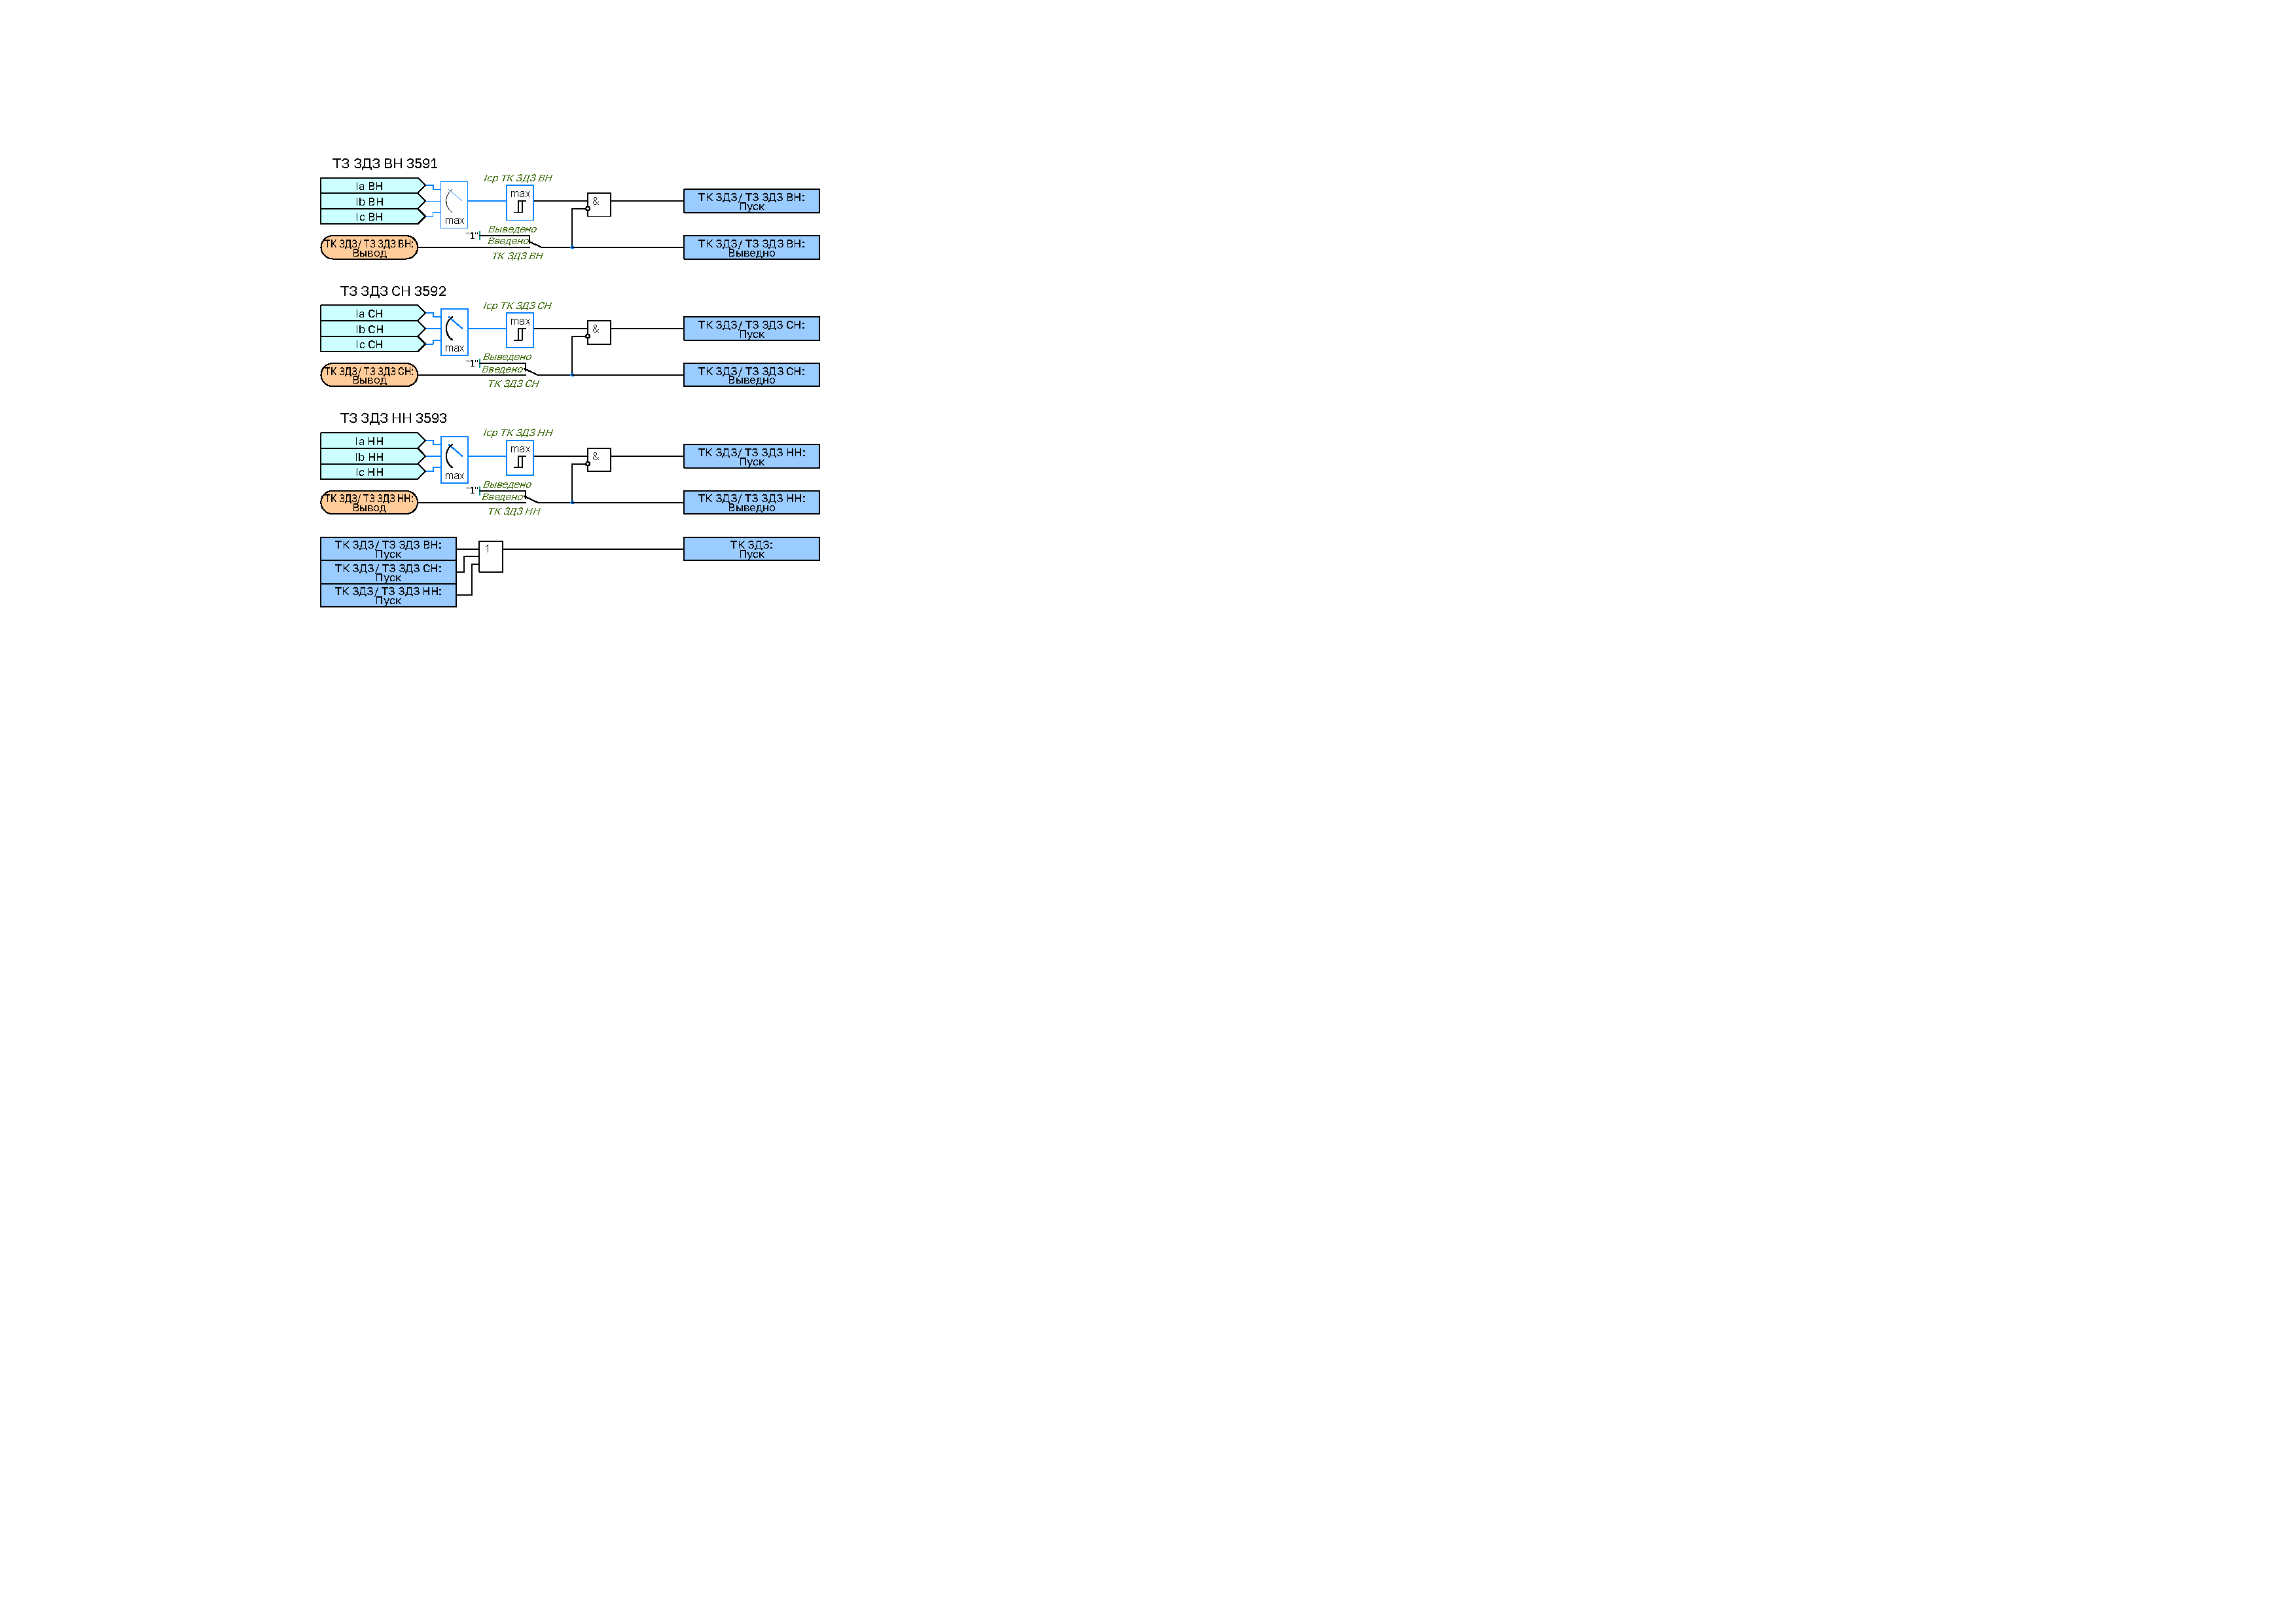
\includegraphics[width=0.75\textwidth,height=0.75\textheight,keepaspectratio]{img17.pdf}
\captionof{figure}{Функциональная схема логики ТК ЗДЗ}\label{pic:ZDZ}
\end{figure}


\end{enumerate}\color{unidarkgreen}{\subsection{Автоматика пуска пожаротушения}}
\color{black}

\begin{enumerate}[label=\arabic{section}.\arabic{subsection}.\arabic*,  align=left, labelsep=4pt, leftmargin=0pt, itemindent=57pt]

\item
Устройство осуществляет выдачу сигнала пуска пожаротушения автотрансформатора. Пуск пожаротушения АТ осуществляется при срабатывании дифференциальной защиты или газовой защиты АТ на отключение.
Минимальная длительность импульса выходного сигнала пуска пожаротушения АТ определяется уставкой \textbf{«Tимп АПТ»}.

\item
Алгоритм работы логики пуска АПТ приведен на рисунке \ref{pic:APT}. Уставки ТК ЗДЗ приведены в таблице \ref{app_set:apt}.

\begin{figure}[H]
\centering
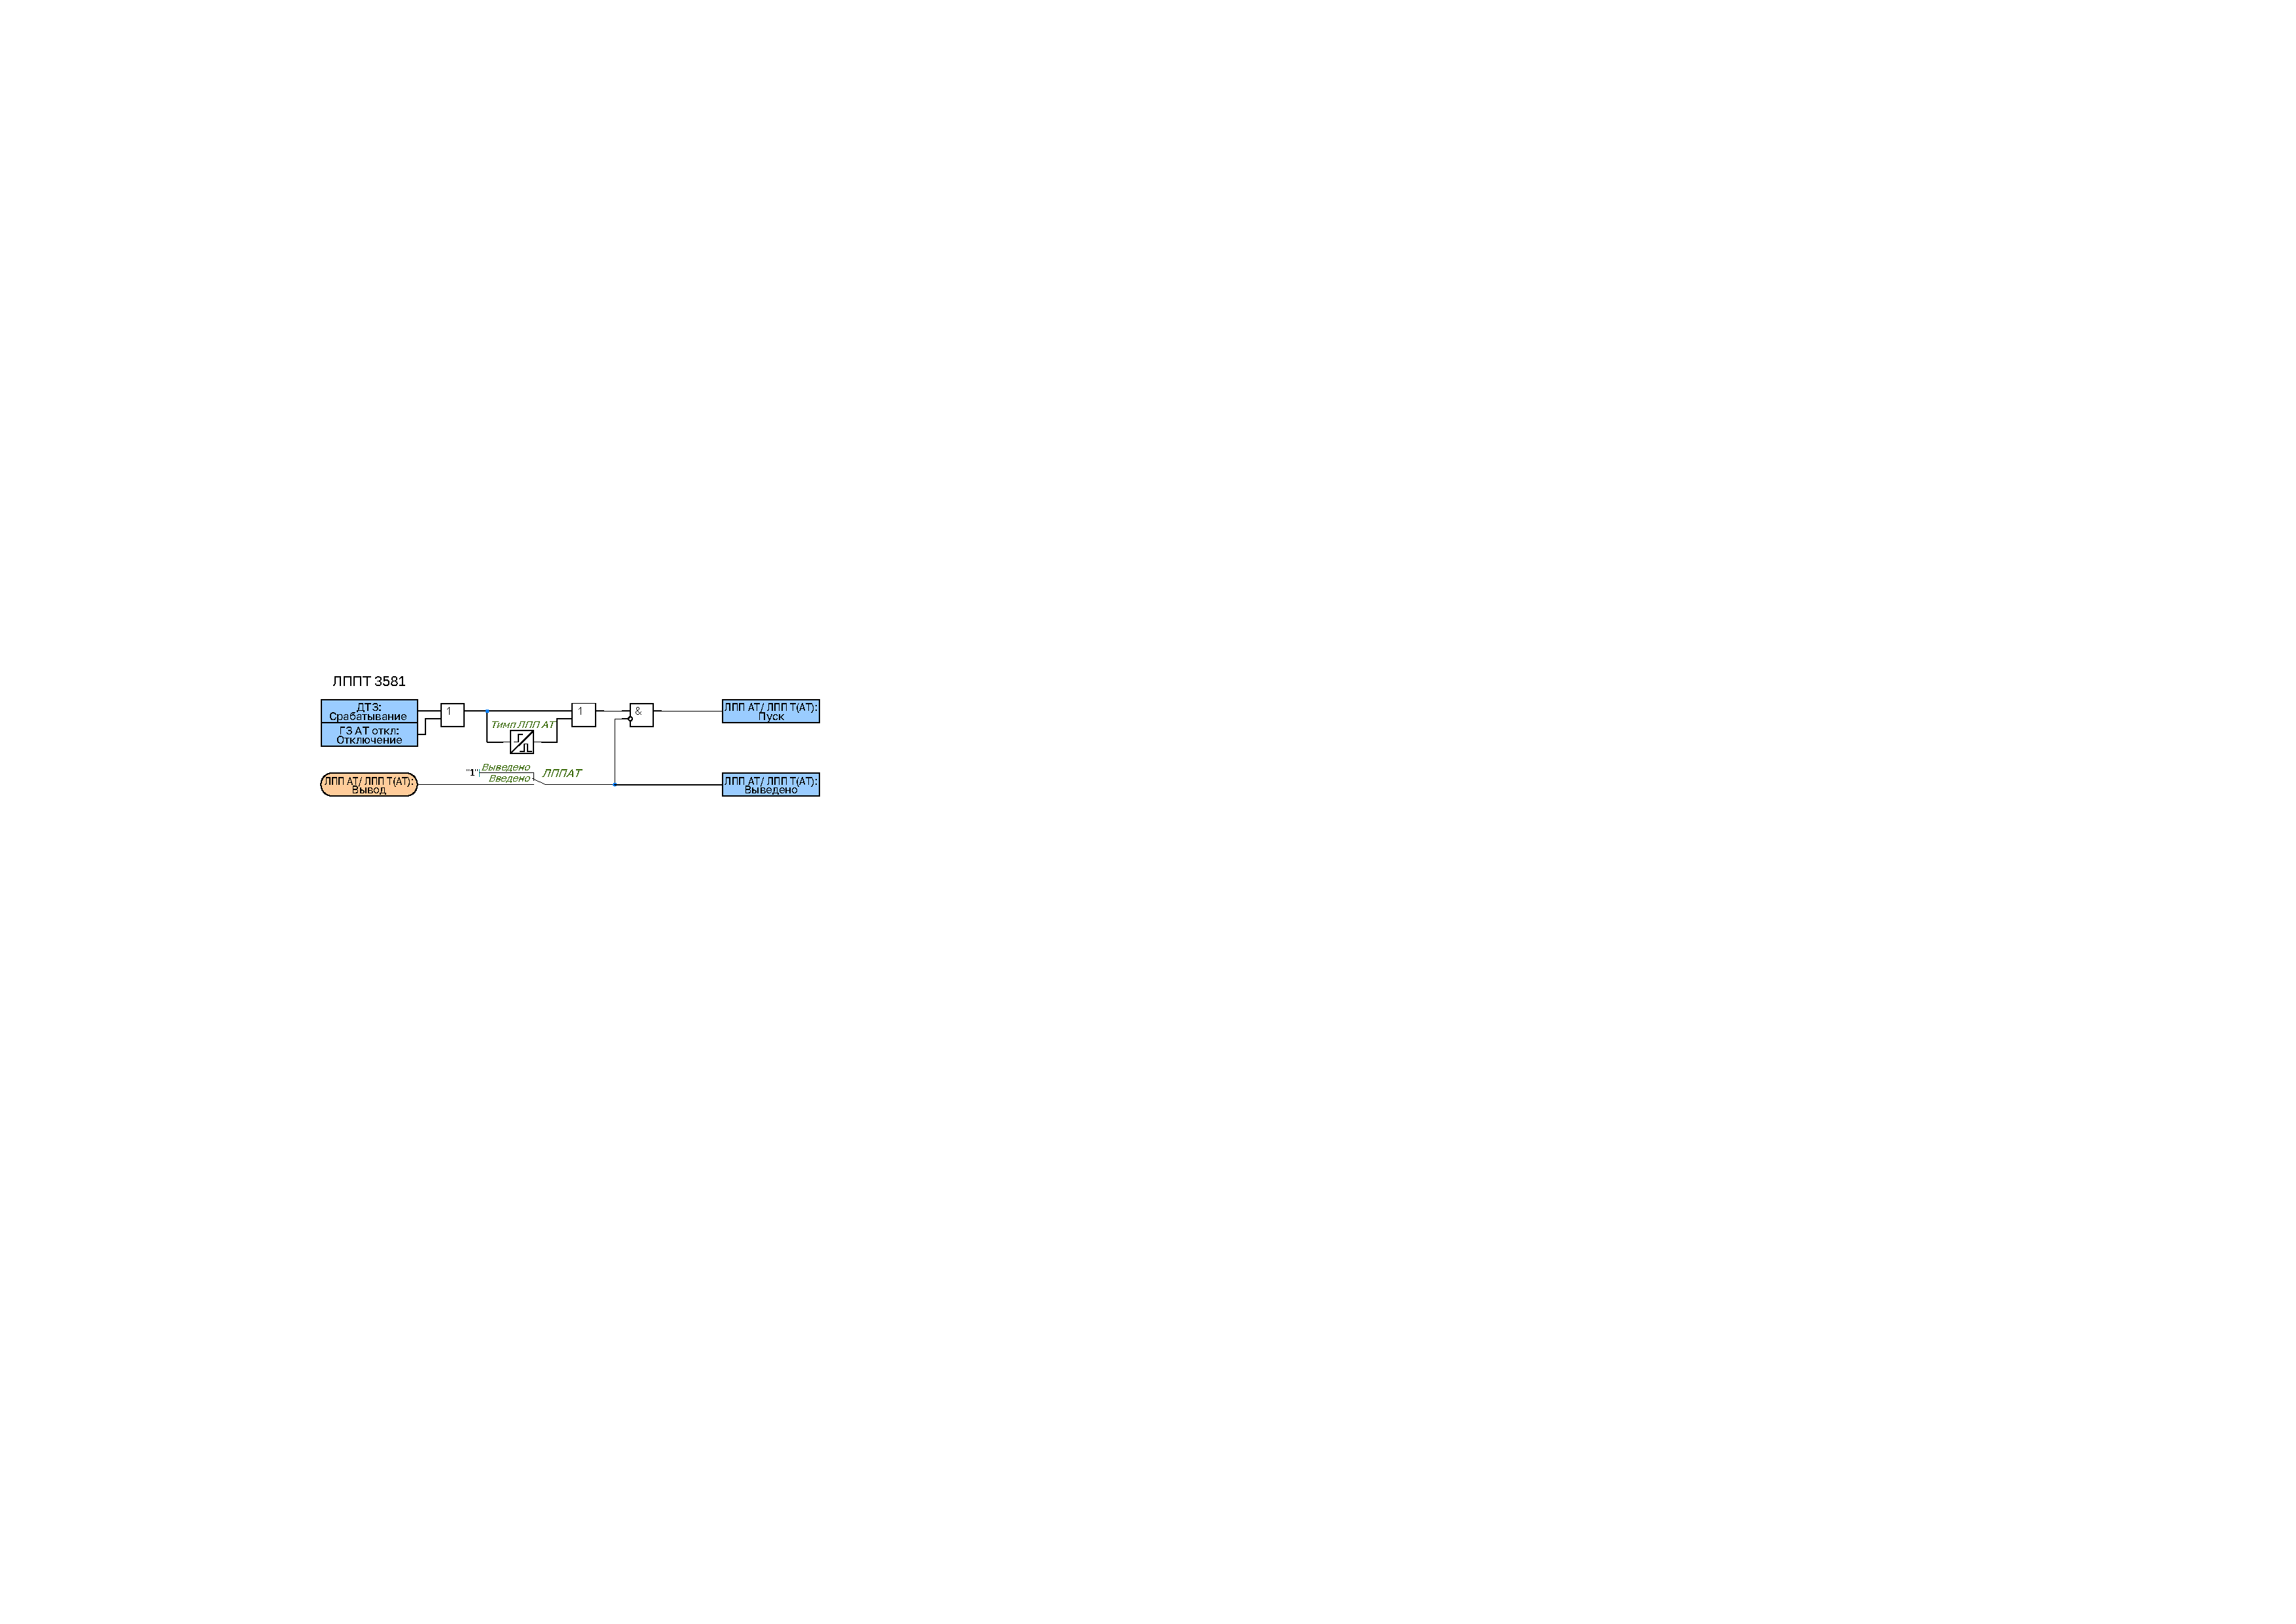
\includegraphics[width=0.85\textwidth,height=0.85\textheight,keepaspectratio]{img18.pdf}
\captionof{figure}{Функциональная схема логики пуска АПТ}\label{pic:APT}
\end{figure}


\end{enumerate}
\needspace{2\baselineskip}
\color{unidarkgreen}{\subsection{Контроль отсутствия напряжения}}
\color{black}

\begin{enumerate}[label=\arabic{section}.\arabic{subsection}.\arabic*,  align=left, labelsep=4pt, leftmargin=0pt, itemindent=57pt]

\item
Для исключения пуска пожаротушения не отключенного от сети трансформатора обеспечиваются следующие виды контроля:
\begin{itemize}
\item отсутствие тока на стороне ВН;
\item отсутствие тока на стороне СН;
\item отсутствие напряжения на стороне НН.
\end{itemize}

\item
Алгоритм работы КОН приведен на рисунке \ref{pic:KON}. Уставки КОН приведены в таблице \ref{app_set:kon}.

\vspace{2mm}
\begin{figure}[H]
\centering
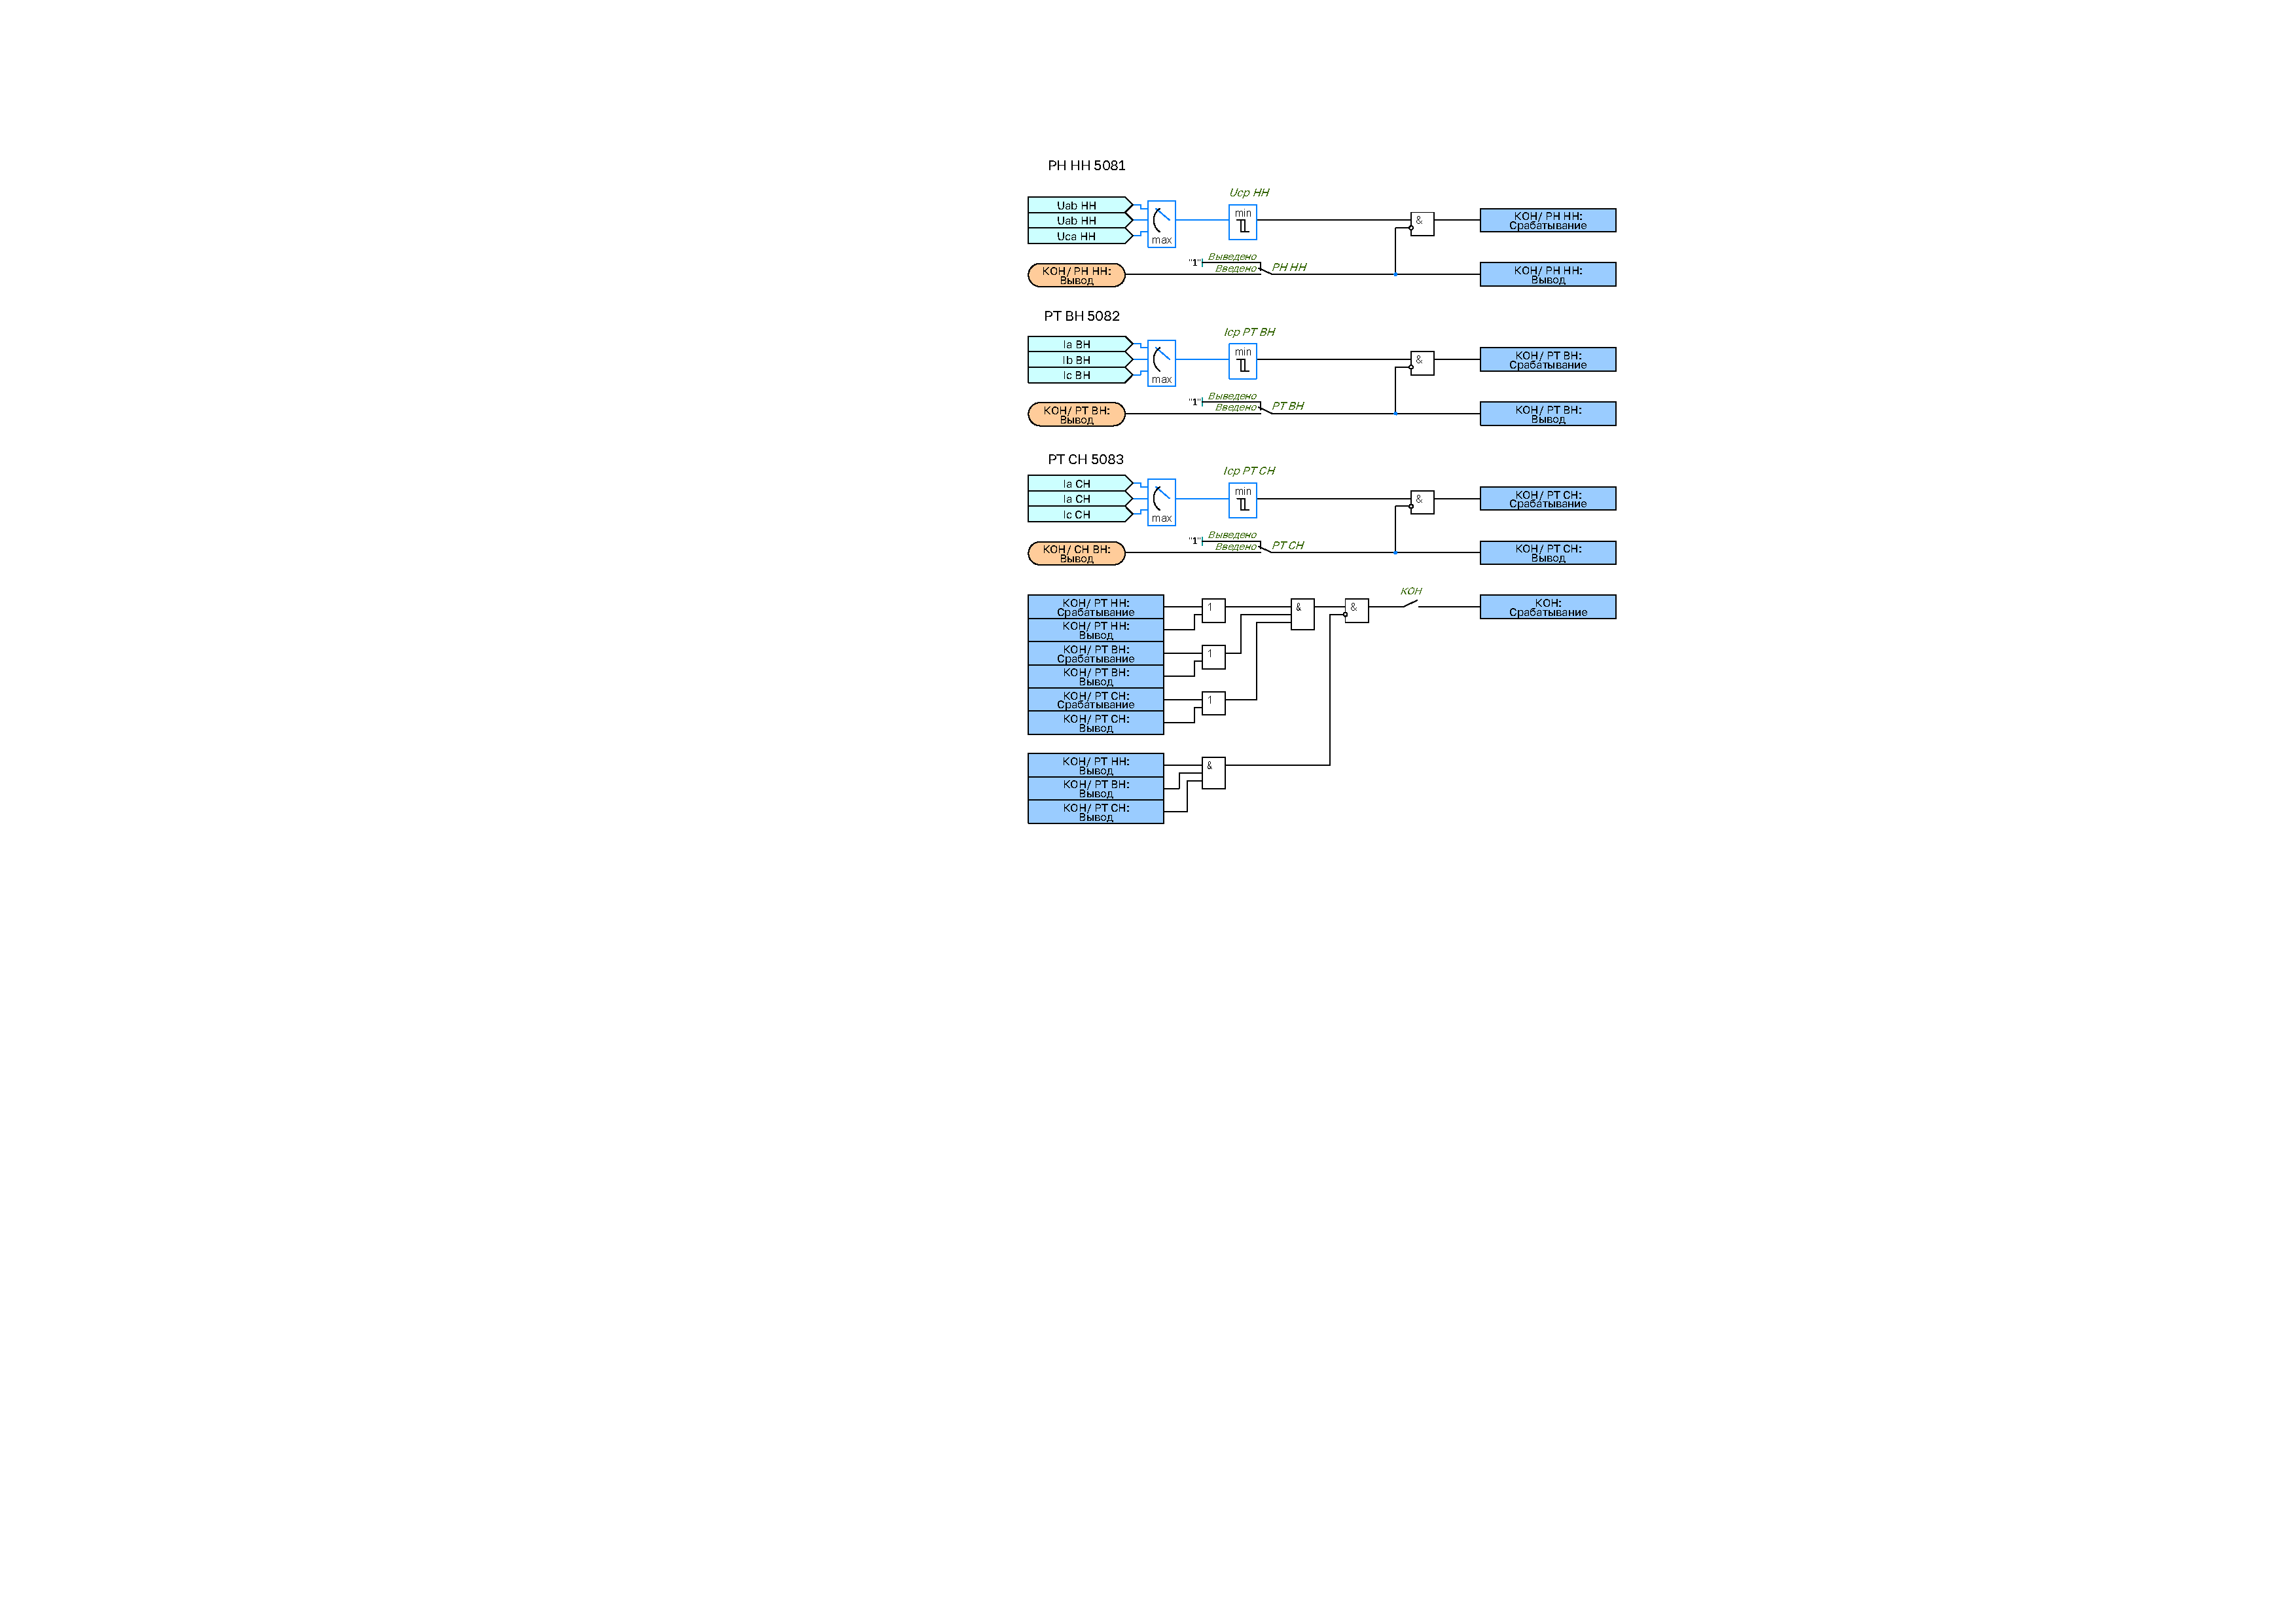
\includegraphics[width=0.8\textwidth,height=0.8\textheight,keepaspectratio]{img19.pdf}
\captionof{figure}{Функциональная схема логики КОН}\label{pic:KON}
\end{figure}


\end{enumerate}
\color{unidarkgreen}{\subsection{Реле тока пуска охлаждения}}
\color{black}

\begin{enumerate}[label=\arabic{section}.\arabic{subsection}.\arabic*,  align=left, labelsep=4pt, leftmargin=0pt, itemindent=57pt]

\item
Охлаждающие устройства в системах охлаждения мощных автотрансформаторов разбиты на несколько групп, которые последовательно включаются в работу в зависимости от изменения условий работы автотрансформатора. Функция пуска охладителей контролирует уровни тока на обмотках ВН, НН, а также на общей обмотке автотрансформатора. 

\item
К каждой из обмоток подключено по два реле тока для пуска групп охладителей. Каждое реле имеет индивидуально настраиваемый порог по току срабатывания, задаваемый пользователем.

\item
Уставки функций в составе РТПО приведены в таблице \ref{app_set:rtpo}.

\item
На рисунке \ref{pic:RTPO} представлена схема реле тока пуска охлаждения для обмотки ВН. Схема реле тока пуска охлаждения для общей обмотки автотрансформатора и обмотки НН выполнена аналогично.

\begin{figure}[H]
\centering
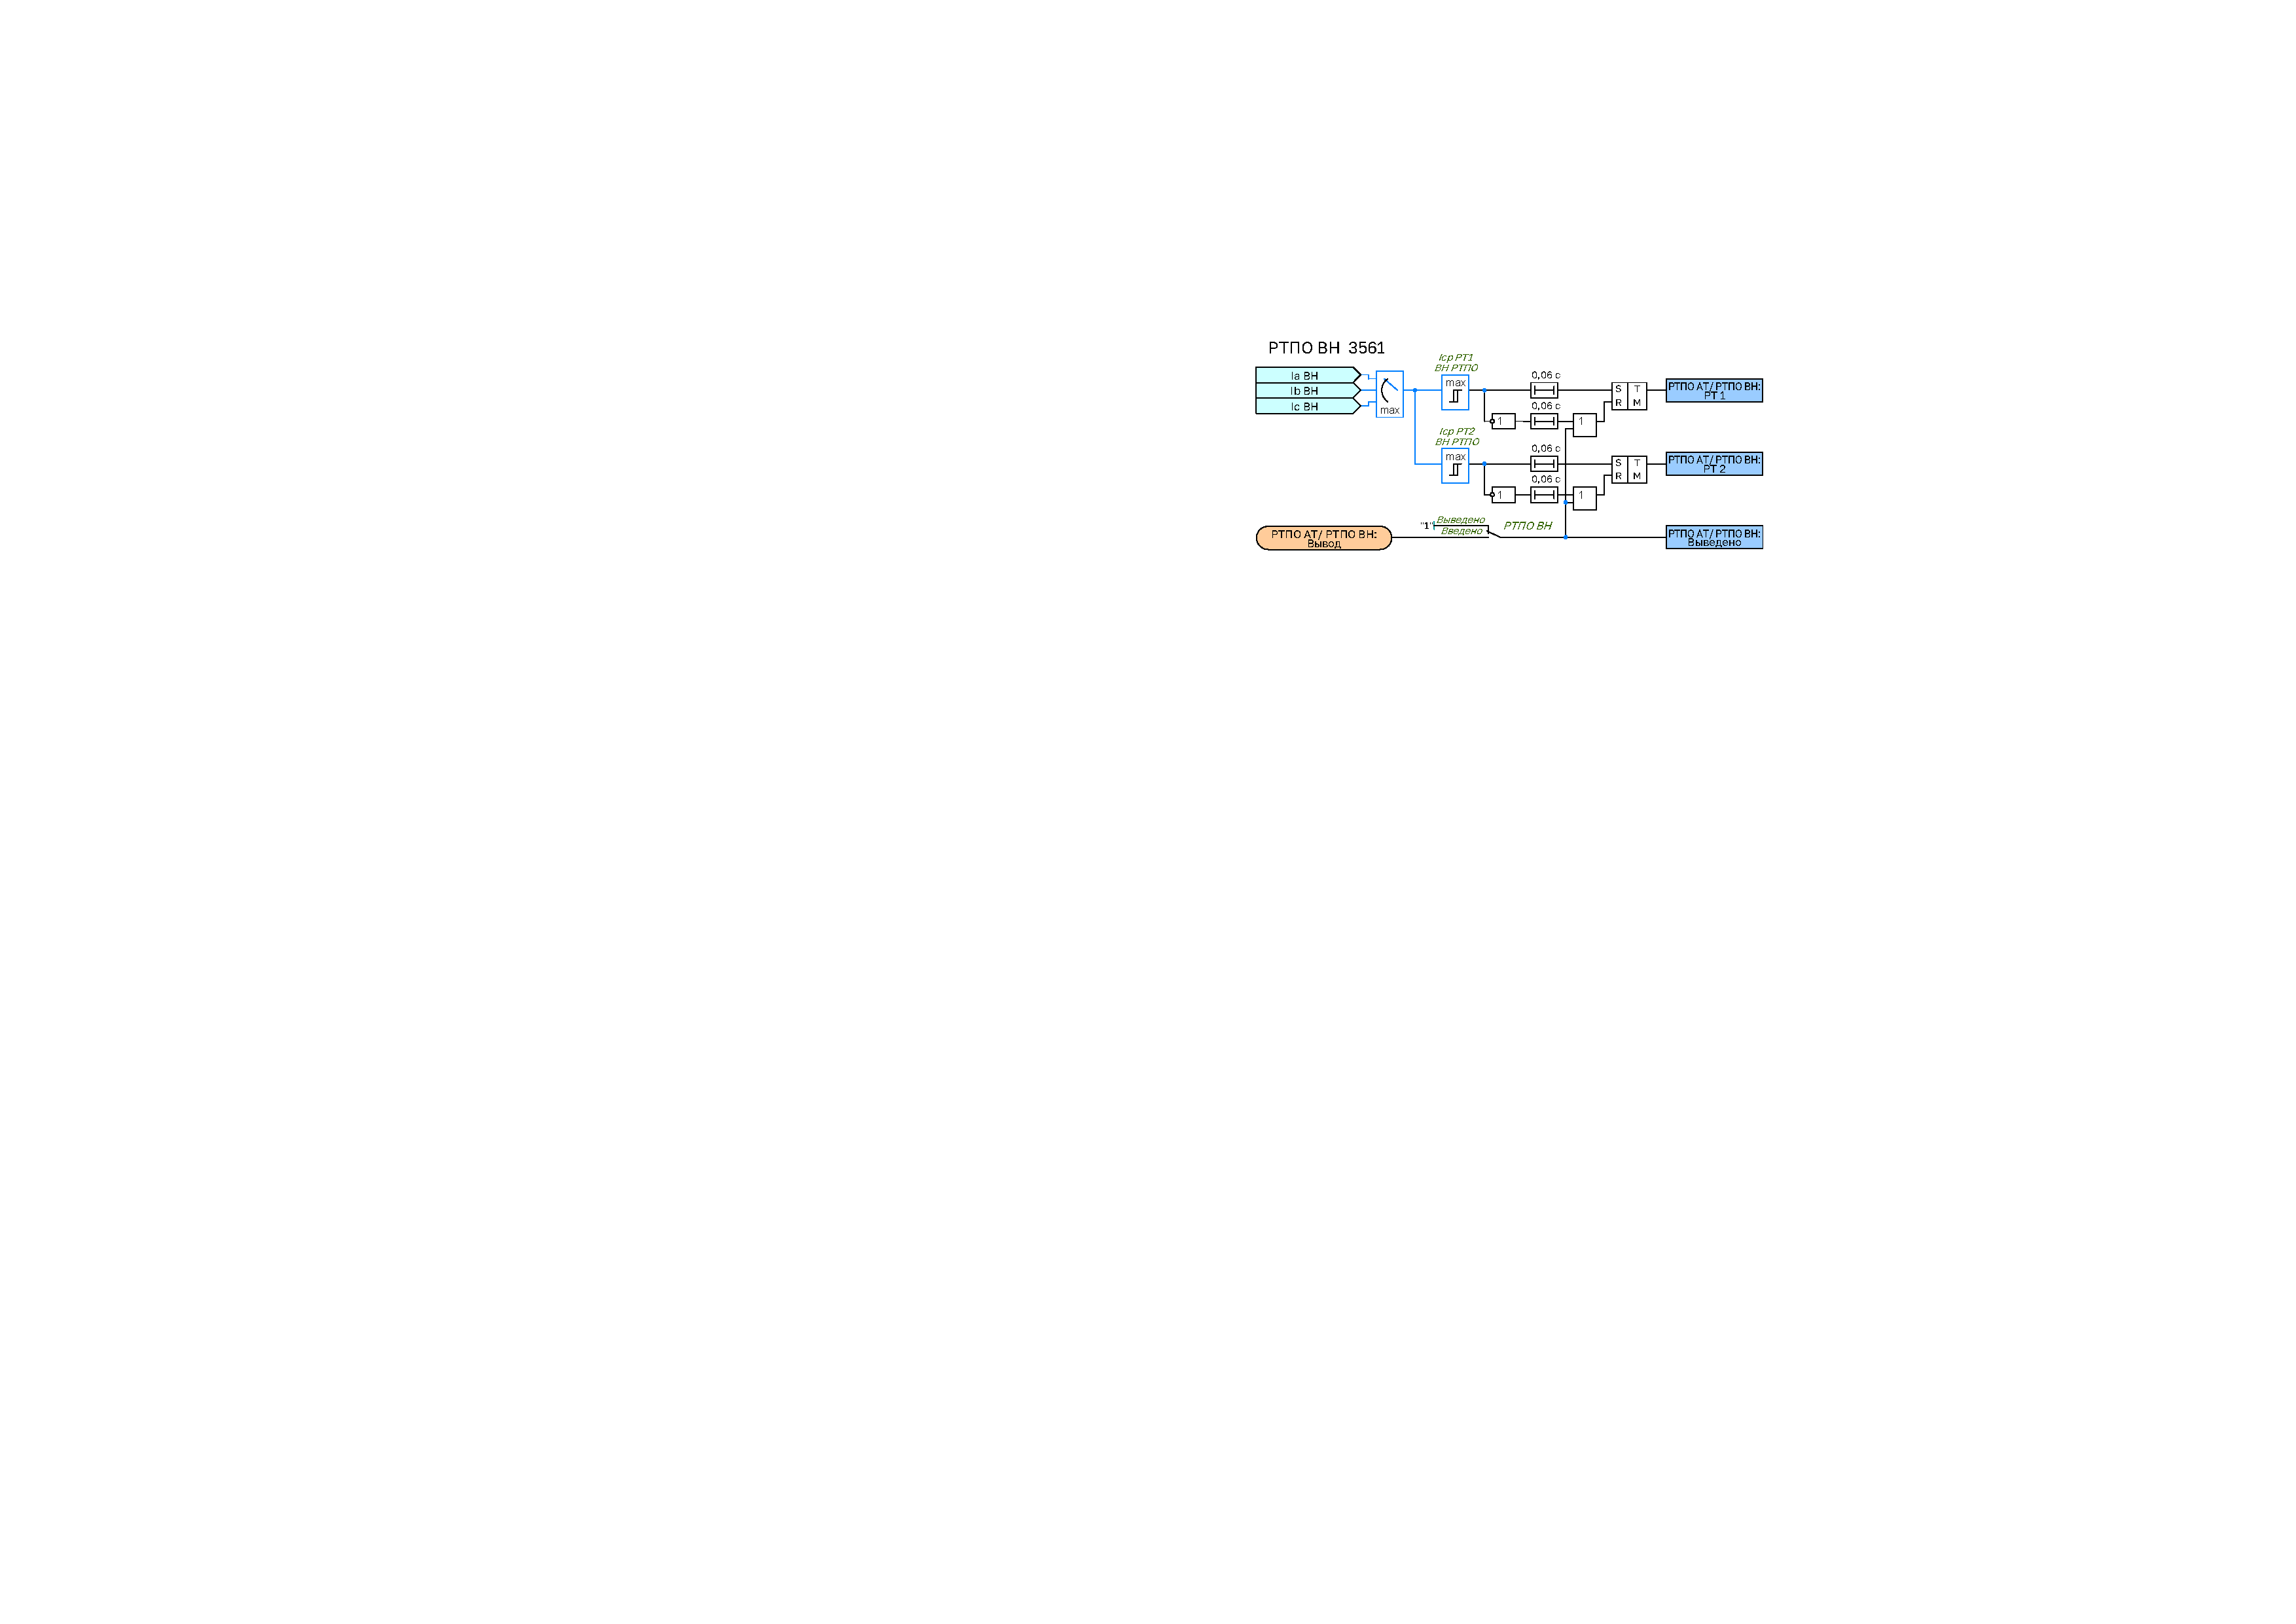
\includegraphics[width=0.9\textwidth,height=0.9\textheight,keepaspectratio]{img20.pdf}
\captionof{figure}{Функциональная схема логики РТПО ВН}\label{pic:RTPO}
\end{figure}


\end{enumerate}\color{unidarkgreen}{\subsection{Реле тока блокировки РПН}}
\color{black}

\begin{enumerate}[label=\arabic{section}.\arabic{subsection}.\arabic*,  align=left, labelsep=4pt, leftmargin=0pt, itemindent=57pt]

\item
В целях блокирования автоматики РПН при превышении током через РПН допустимого значения предусматривается реле блокировки. По умолчанию данное реле подключено к трансформаторам тока стороны СН автотрансформатора. Порог по току срабатывания реле задается параметром \textbf{«Iбл РПН»}.

\item
Алгоритм работы РТ РПН приведен на рисунке \ref{pic:rtrpn}. Уставки РТ РПН приведены в таблице \ref{app_set:rtrpn}.

\vspace{2mm}
\begin{figure}[H]
\centering
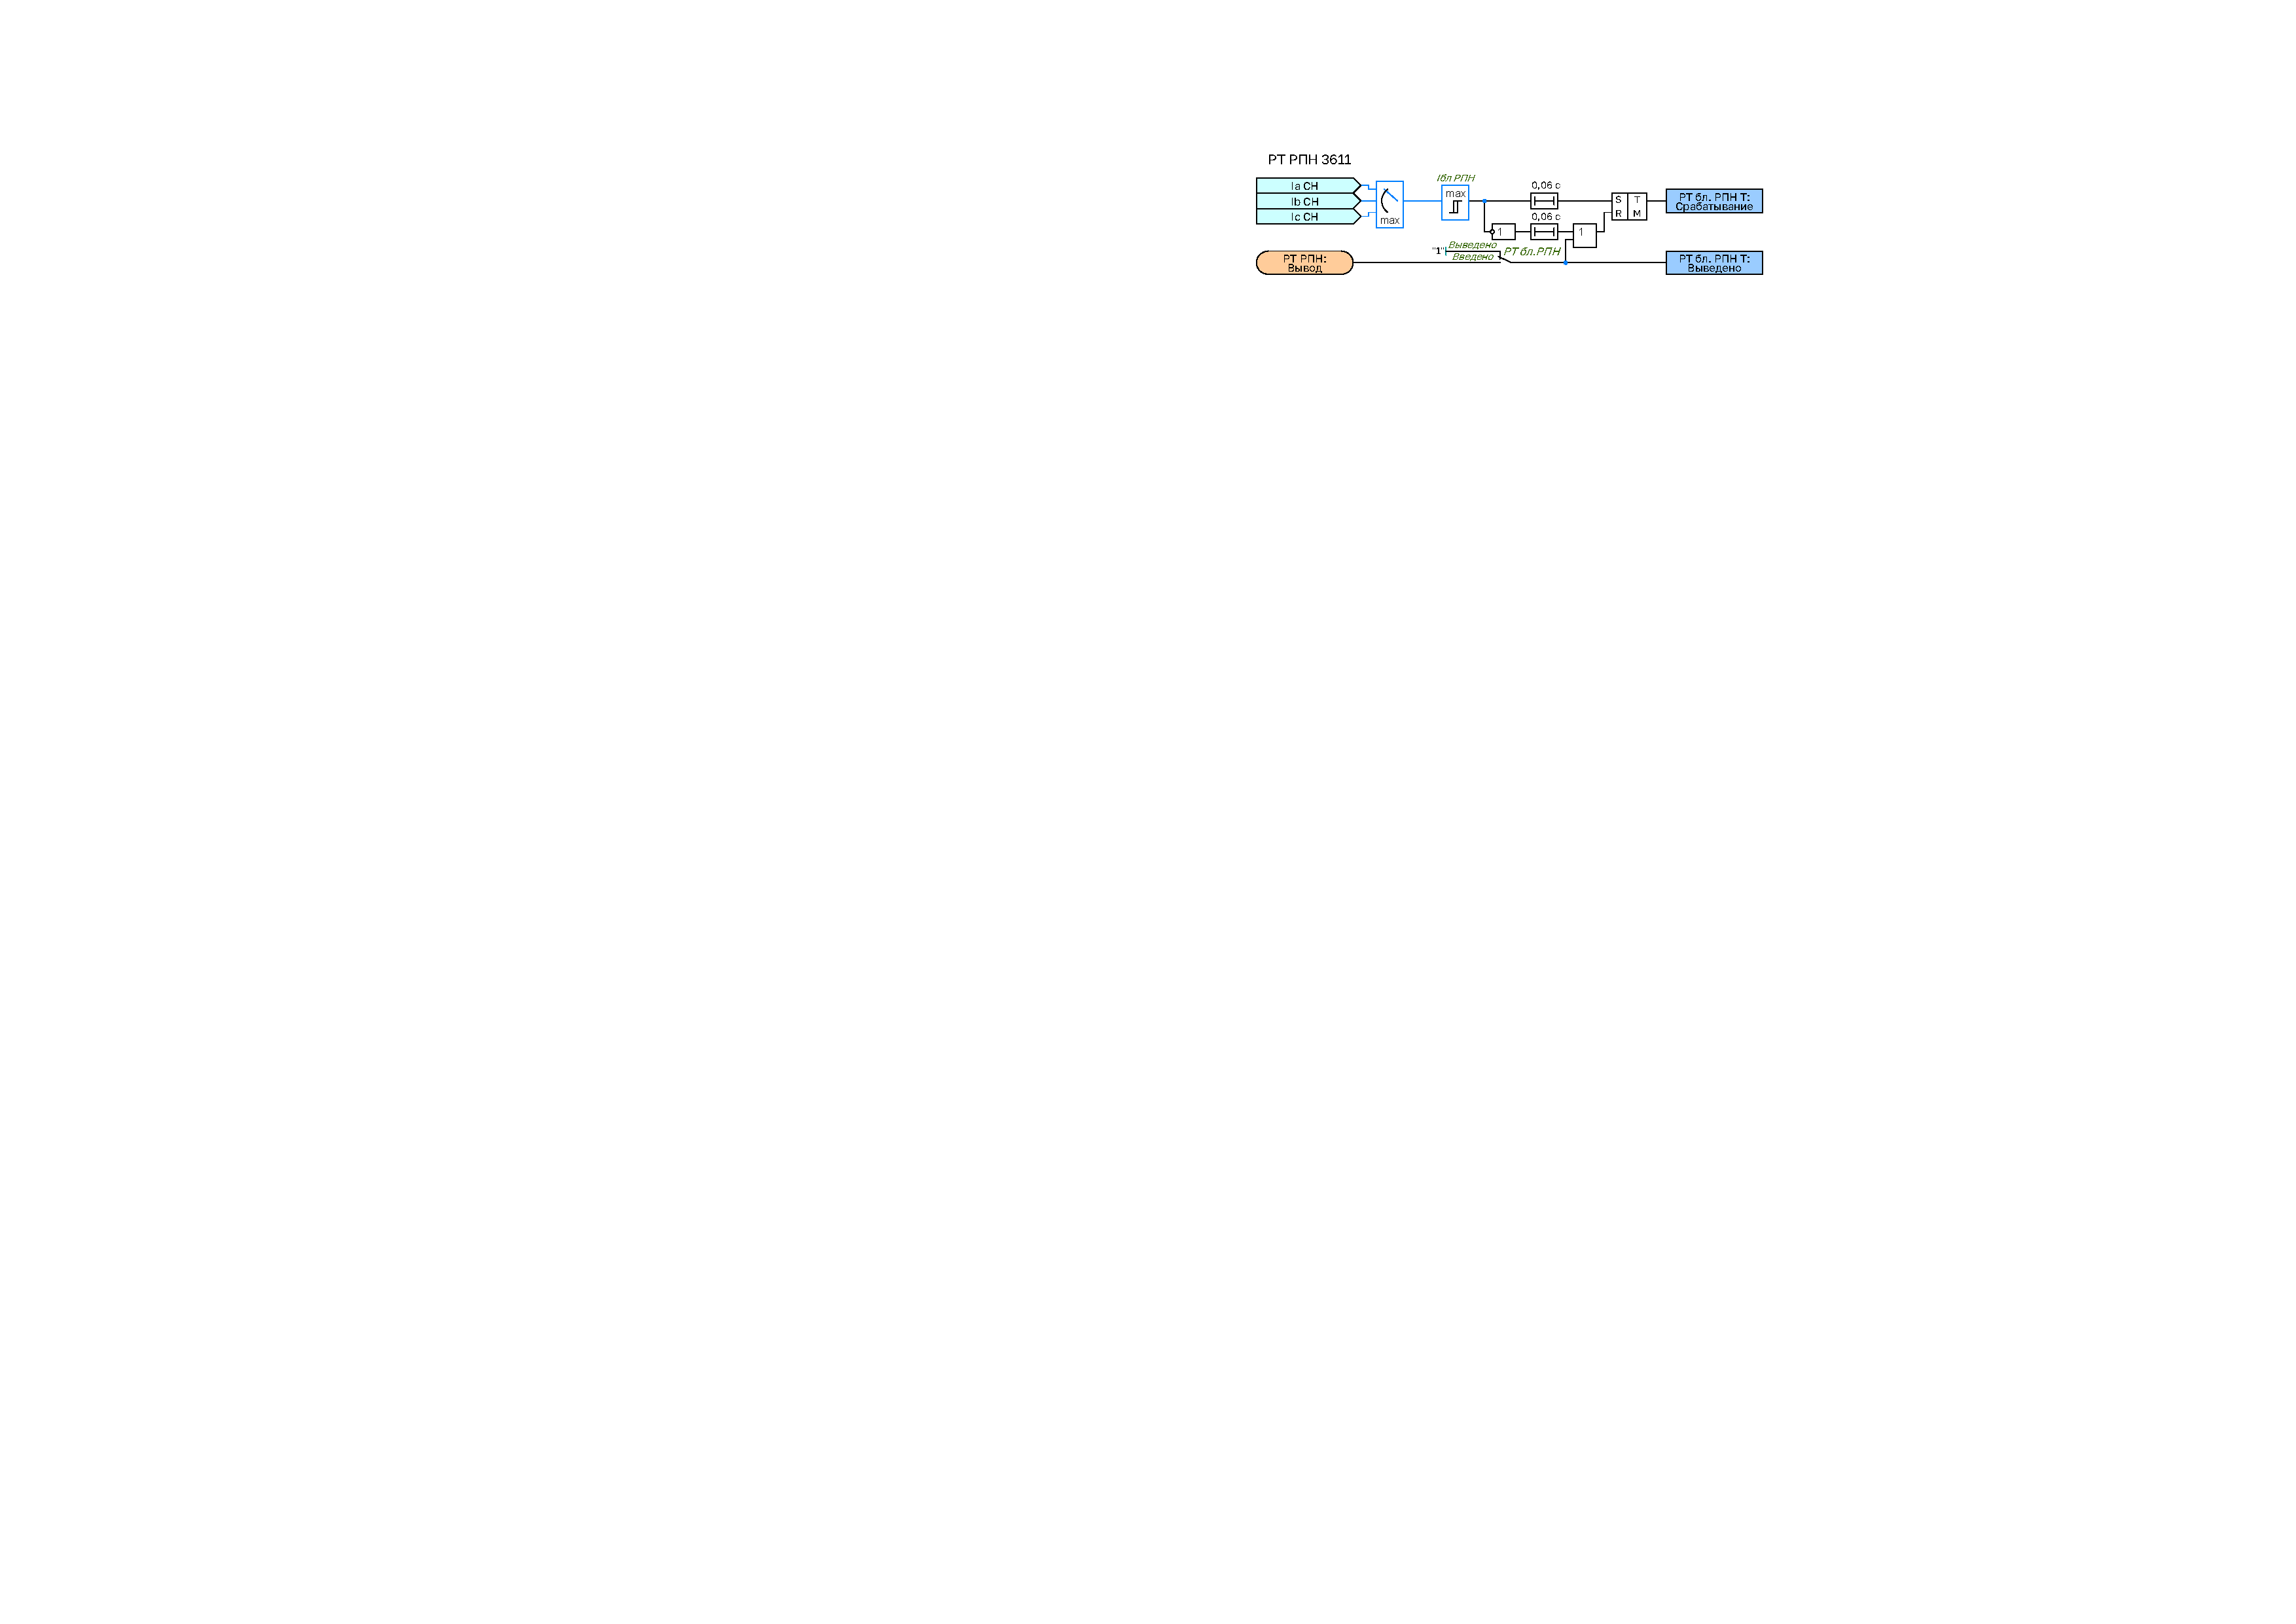
\includegraphics[width=0.9\textwidth,height=0.9\textheight,keepaspectratio]{img21.pdf}
\captionof{figure}{Функциональная схема логики РТ блокировки РПН}\label{pic:rtrpn}
\end{figure}

\end{enumerate}
\color{unidarkgreen}{\subsection{Защита от перегрузки}}
\color{black}

\begin{enumerate}[label=\arabic{section}.\arabic{subsection}.\arabic*,  align=left, labelsep=4pt, leftmargin=0pt, itemindent=57pt]

\item
Защита от перегрузки (ЗП) предназначена для контроля нагрузки трансформатора с целью предотвращения повреждения оборудования. ЗП подключается к фазным токам сторон ВН и НН автотрансформатора, а также к расчетным фазным токам общей обмотки автотрансформатора.

\item
ЗП каждой стороны и общей обмотки автотрансформатора состоит из максиселектора фазных токов, максимального органа сравнения с уставкой \textbf{«Iср ЗП»} и выдержки времени \textbf{«Тср ЗП»}, по истечении которой выдается сигнал срабатывания. Предусмотрены ввод/вывод в работу программным переключателем \textbf{«ЗП»} для каждой стороны и общей обмотки автотрансформатора.

\item
Алгоритм работы ЗП приведен на рисунке \ref{pic:zp}. Уставки ЗП приведены в таблице \ref{app_set:zp}.

\vspace{2mm}
\begin{figure}[H]
\centering
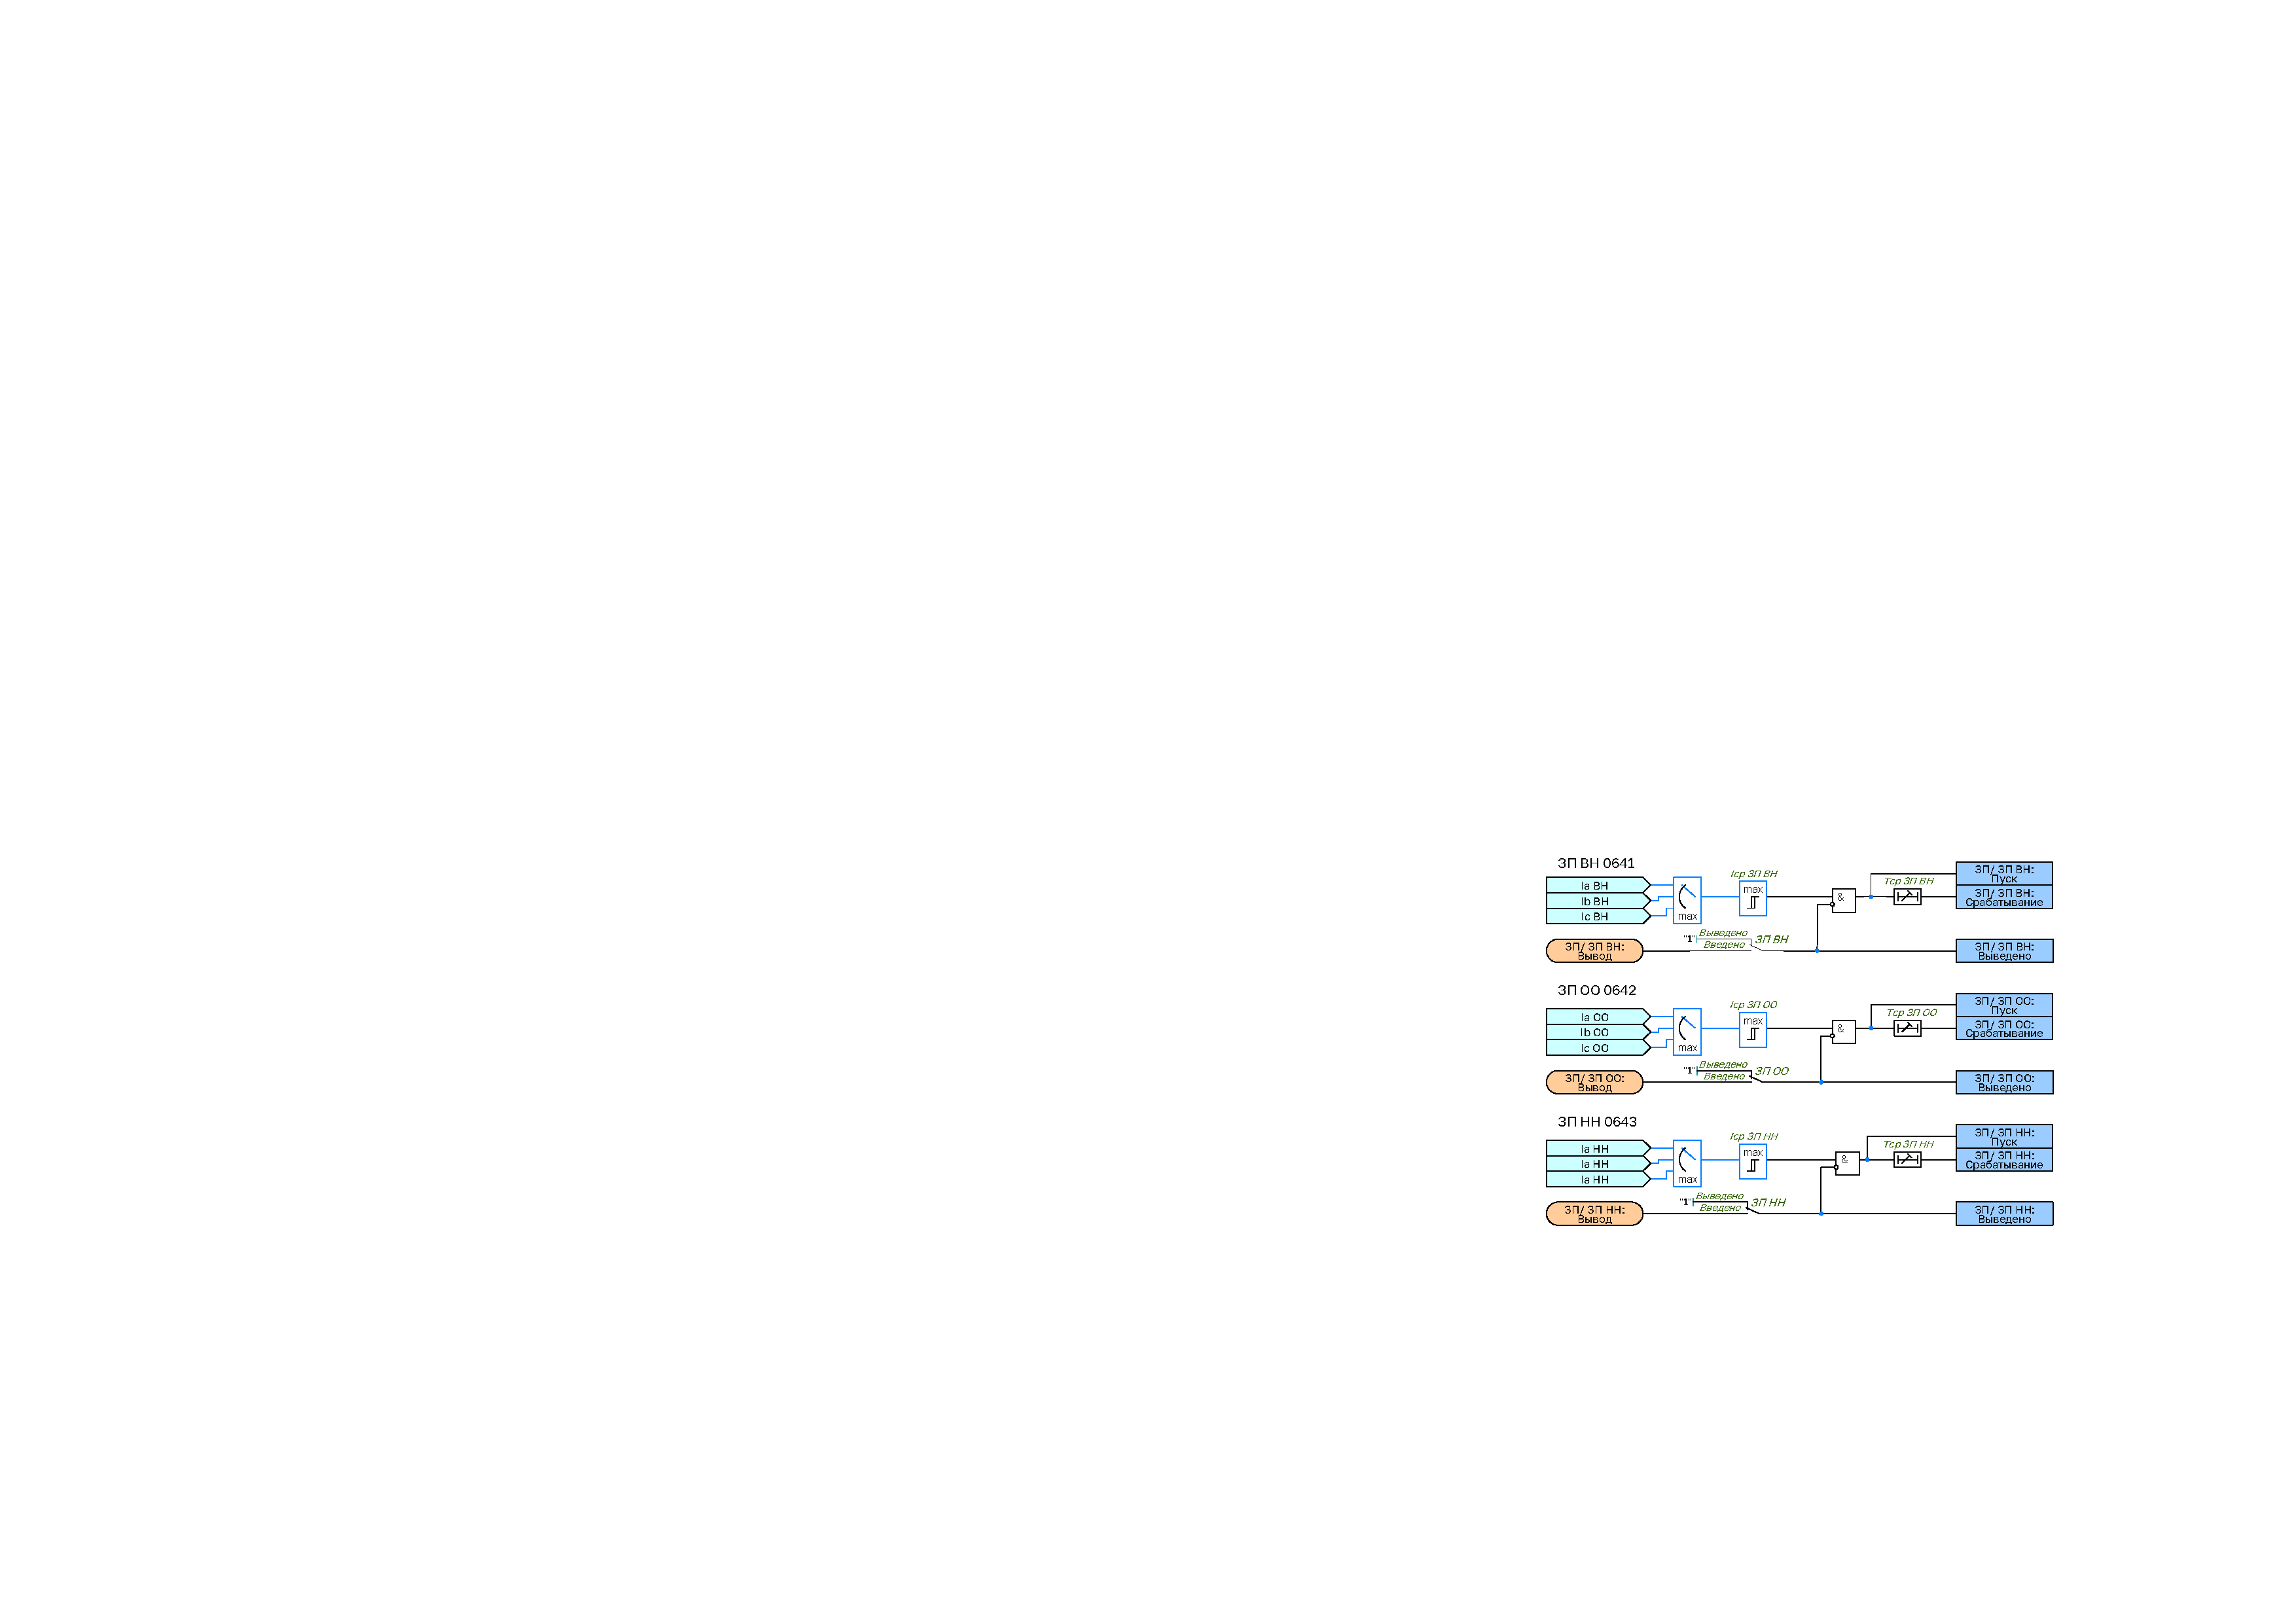
\includegraphics[width=0.8\textwidth,height=0.8\textheight,keepaspectratio]{img22.pdf}
\captionof{figure}{Функциональная схема логики ЗП}\label{pic:zp}
\end{figure}

\end{enumerate}
\color{unidarkgreen}{\subsection{Защита от потери охлаждения}}
\color{black}

\begin{enumerate}[label=\arabic{section}.\arabic{subsection}.\arabic*,  align=left, labelsep=4pt, leftmargin=0pt, itemindent=57pt]

\item
Защита от потери охлаждения направлена на предотвращение перегрева и повреждения первичного оборудования (автотрансформатора, шунтирующего ректора) в результате частичного или полного отказа системы охлаждения.

\item
Функция защиты от потери охлаждения контролирует уровни тока в обмотках ВН, НН, а также в общей обмотке автотрансформатора. К каждой из обмоток подключено по два реле тока для контроля за уровнем нагрузки автотрансформатора. Каждое реле имеет индивидуально настраиваемый порог по току срабатывания, задаваемый пользователем.

\item
Защита содержит три ступени, каждая из которых может быть выполнена с контролем температуры масла и уровня тока. Ввод контроля перегрева масла, а также выбор соответствующего уровня тока осуществляется программными накладками \textbf{«ЗПО-N конт.ДТм»} и \textbf{«ЗПО-N конт.РТ»} соответственно (где N – номер ступени). Каждая из ступеней имеет индивидуальную регулируемую задержку на срабатывание.

\item
Алгоритм работы ЗПО приведен на рисунке \ref{pic:ZPO}. Уставки ЗПО приведены в таблице \ref{app_set:zpo}.

\begin{figure}[H]
\centering
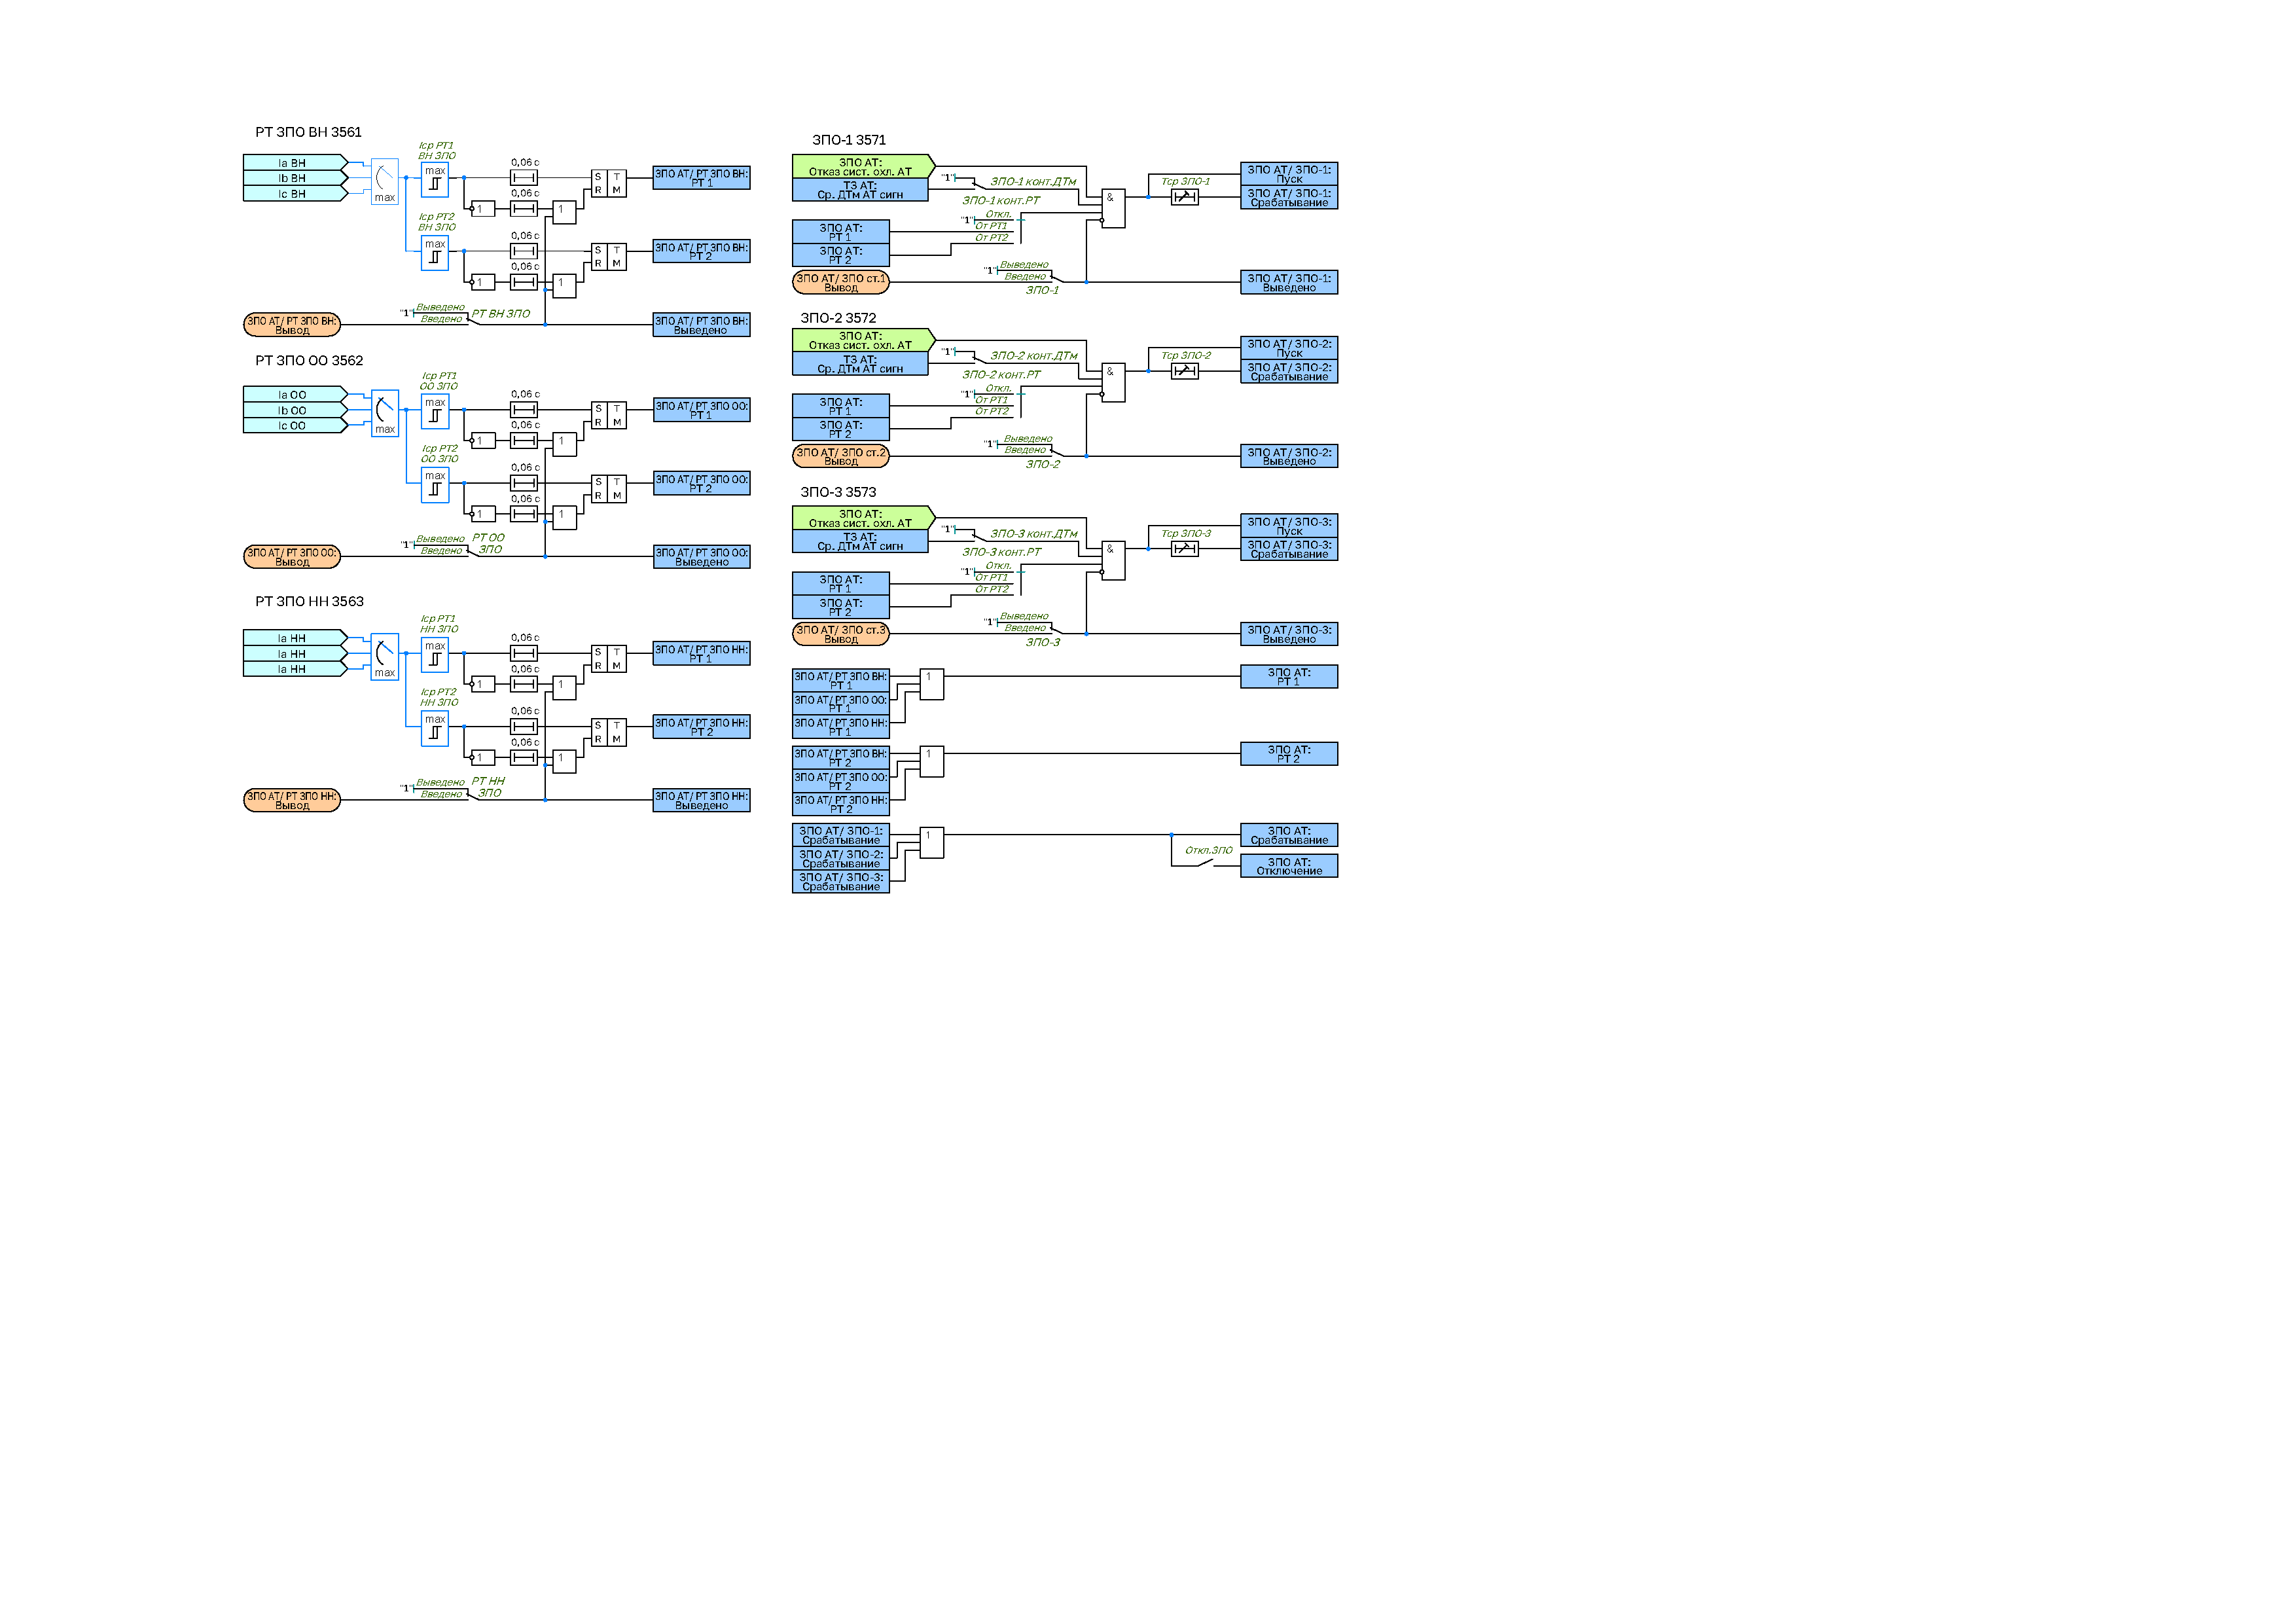
\includegraphics[width=1\textwidth,height=1\textheight,keepaspectratio]{img23.pdf}
\captionof{figure}{Функциональный блок ЗПО}\label{pic:ZPO}
\end{figure}

\end{enumerate}
\color{unidarkgreen}{\subsection{Контроль изоляции стороны НН}}
\color{black}

\begin{enumerate}[label=\arabic{section}.\arabic{subsection}.\arabic*,  align=left, labelsep=4pt, leftmargin=0pt, itemindent=57pt]

\item
Для информирования персонала при возникновении однофазного замыкания на землю предусмотрен сигнальный орган контроля изоляции, контролирующий значение утроенного напряжения нулевой последовательности ($3U_0$). 

\item
Значение срабатывания по напряжению нулевой последовательности, определяемое параметром \textbf{«3U0ср КИ НН»}. Для исключения ложного формирования сигнализации при возникновении неисправности цепей напряжения предусмотрен блокирующий орган, включенный на напряжение обратной последовательности. Значение блокировки по напряжению обратной последовательности задается параметром \textbf{«U2бл КИ НН»}. Действие на сигнализацию формируется с задержкой по времени \textbf{«Тср КИ НН»}.

\item
Алгоритм работы КИ НН приведен на рисунке \ref{pic:KINN}. Уставки КИ НН приведены в таблице \ref{app_set:kinn}.

\vspace{2mm}
\begin{figure}[H]
\centering
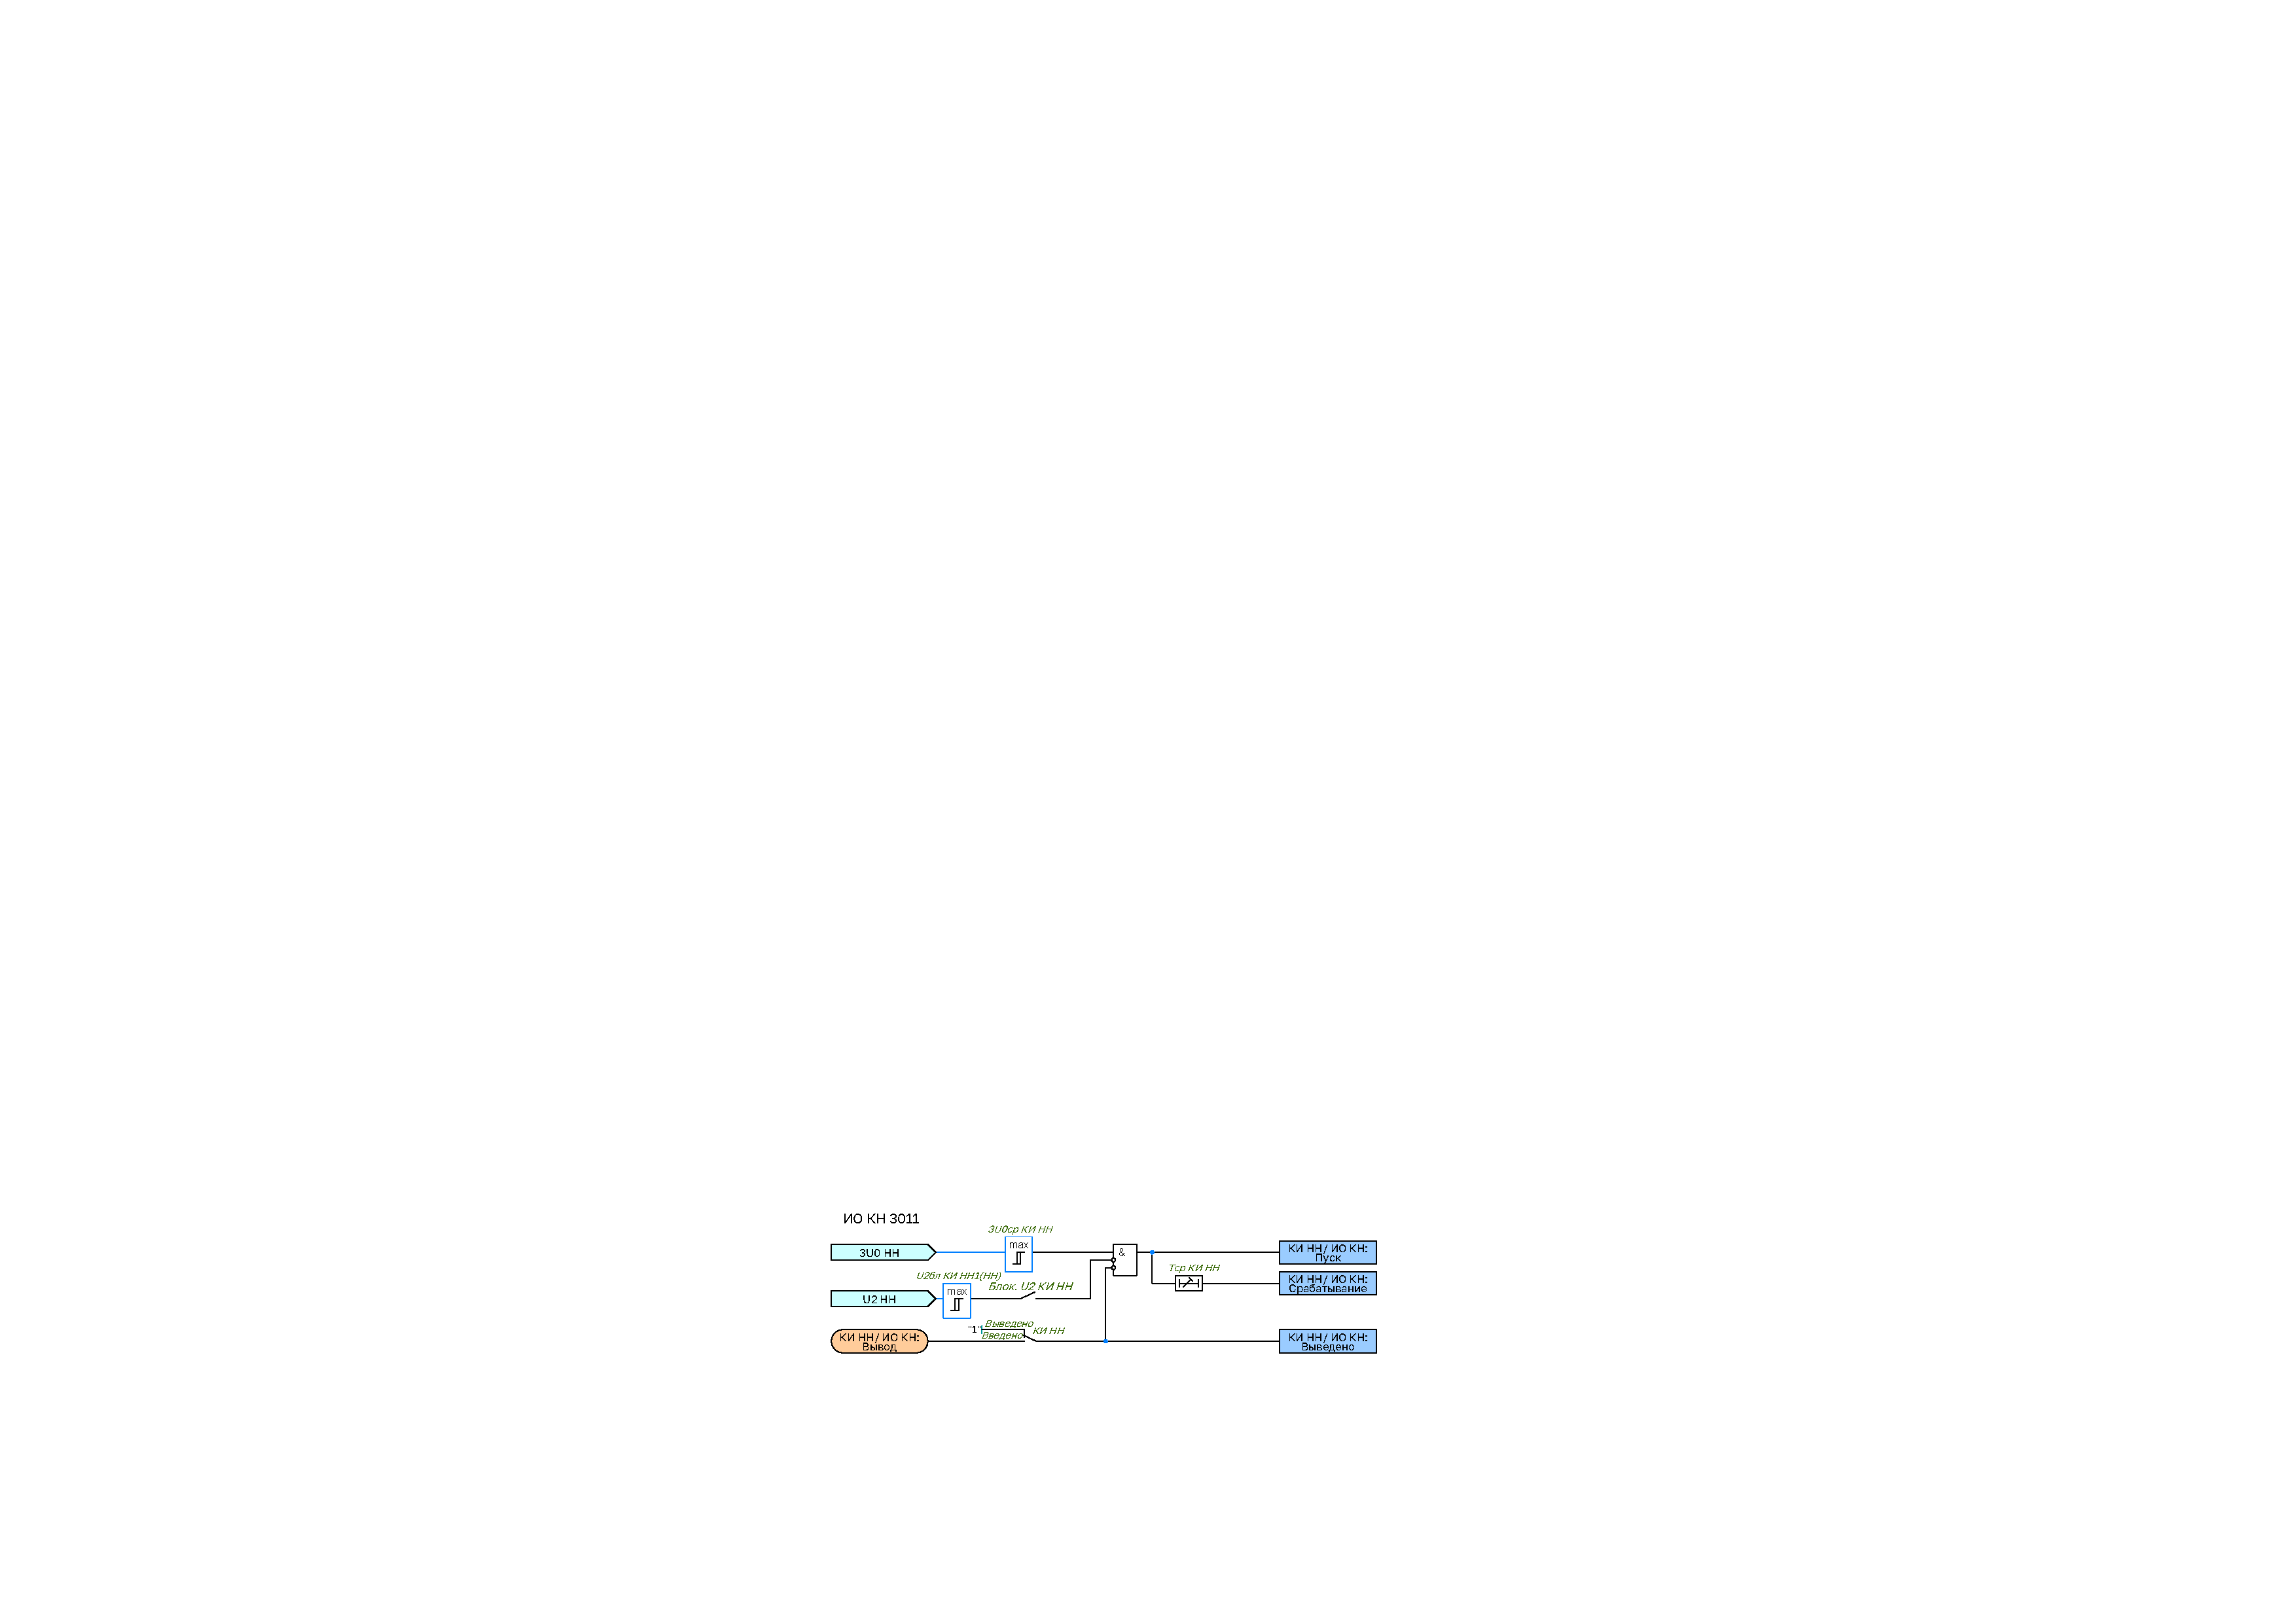
\includegraphics[width=1\textwidth,height=1\textheight,keepaspectratio]{img24.pdf}
\captionof{figure}{Функциональная схема логики КИ НН}\label{pic:KINN}
\end{figure}

\end{enumerate}
\color{unidarkgreen}{\subsection{Контроль цепей напряжения стороны НН}}
\color{black}

\begin{enumerate}[label=\arabic{section}.\arabic{subsection}.\arabic*,  align=left, labelsep=4pt, leftmargin=0pt, itemindent=57pt]

\item
Контроль цепей напряжения предназначен для выявления нарушений в цепях напряжения низкой стороны автотрансформатора. Цепи напряжения подключаются к ТН, установленным на шинах НН.

\item
Контроль цепей напряжения низкой и средней стороны трансформатора основан на выявлении нарушения симметрии в цепях напряжения и просадки линейного напряжения соответствующей стороны.

\item
Ввод в работу КЦН осуществляется независимо для каждой стороны с помощью уставок \textbf{«КЦН НН», «КЦН НН1» , «КЦН НН2»}. Оперативный ввод/вывод КЦН производится с помощью БУ (блоков управления функциями) «Вывод КЦН НН», «Вывод КЦН НН1», «Вывод КЦН НН2».

\item
Порог срабатывания минимального линейного напряжения задается уставками \textbf{Uл КЦН НН»}, \textbf{Uл КЦН НН1»}, \textbf{Uл КЦН НН2»}. Порог срабатывания максимального напряжения обратной последовательности задается уставками  \textbf{«U2 КЦН НН»}, \textbf{«U2 КЦН НН1»}, \textbf{«U2 КЦН НН2»}. Выдержка времени контроля неисправности цепей напряжения задается уставками \textbf{«Тср КЦН НН»}, \textbf{«Тср КЦН НН1»}, \textbf{«Тср КЦН НН2»}.

\item
Алгоритм работы функций КЦН стороны НН АТ приведен на рисунке \ref{pic:KON}. Уставки функций КЦН НН приведены в таблице \ref{app_set:kznnn1}.

\vspace{2mm}
\begin{figure}[H]
\centering
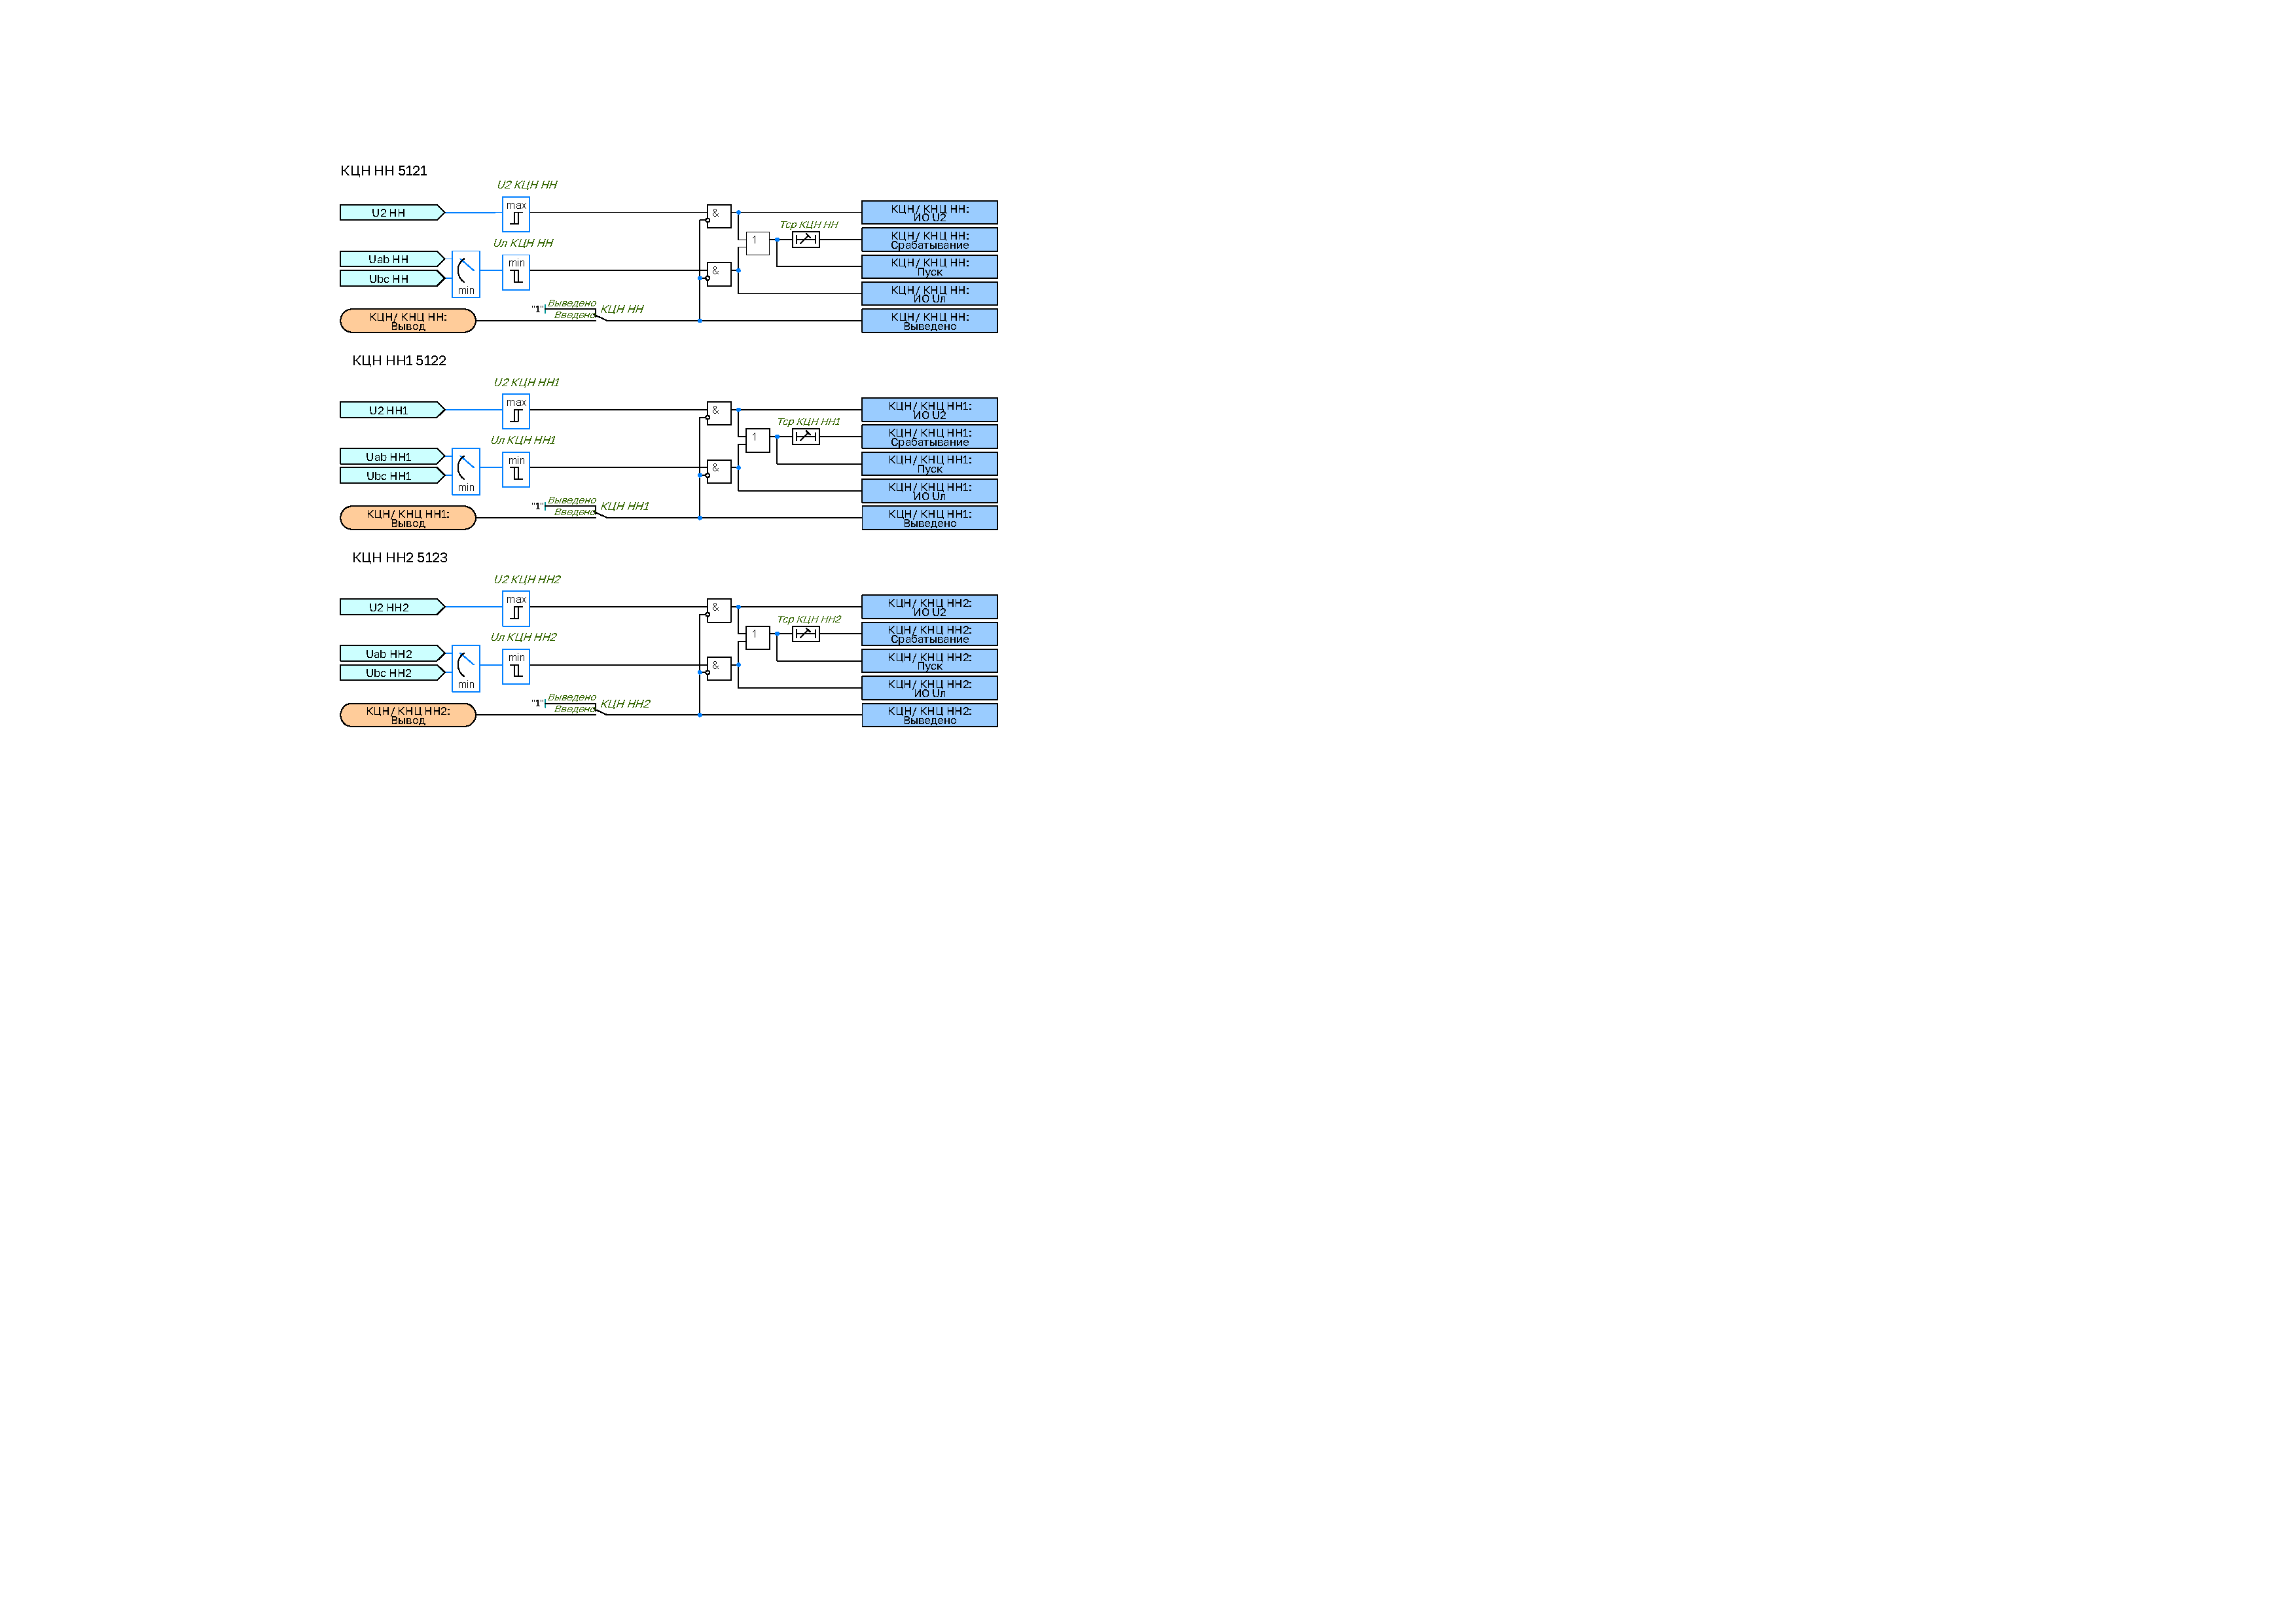
\includegraphics[width=1\textwidth,height=1\textheight,keepaspectratio]{img25.pdf}
\captionof{figure}{Функциональная схема логики функций КЦН стороны НН}\label{pic:KCN}
\end{figure}


\end{enumerate}
\color{unidarkgreen}{\subsection{Устройство резервирования при отказе выключателя}}
\color{black}

\begin{enumerate}[label=\arabic{section}.\arabic{subsection}.\arabic*,  align=left, labelsep=4pt, leftmargin=0pt, itemindent=57pt]

\item
Устройство резервирования при отказе выключателя (УРОВ) предназначено для ликвидации повреждения в случае отказа выключателя поврежденного присоединения.  

\item
Логика работы УРОВ выполнена с контролем протекания тока через выключатель. Значение по току срабатывания задается параметром \textbf{«Iср УРОВ В»}. Функция УРОВ действует с регулируемой задержкой по времени \textbf{«Тср повт. УРОВ»} на повторное отключение своего выключателя, с задержкой \textbf{«Тср УРОВ»} на отключение смежных выключателей.

\item
Действие УРОВ на смежные выключатели может быть выполнено с контролем сигнала РПВ. Ввод контроля сигнала РПВ в логику работы УРОВ осуществляется программной накладкой \textbf{«УРОВ контр. выкл.»}. Предусмотрен подхват по току, включение которого производится программной накладкой \textbf{«УРОВ подхв.»}.

\item
Алгоритм работы УРОВ ВН приведен на рисунке \ref{pic:UROV}. Алгоритм работы УРОВ СН выполнен аналогично. Уставки УРОВ ВН приведены в таблице \ref{app_set:urovvn}. Уставки УРОВ СН приведены в таблице \ref{app_set:urovsn}.

\vspace{2mm}
\begin{figure}[H]
\centering
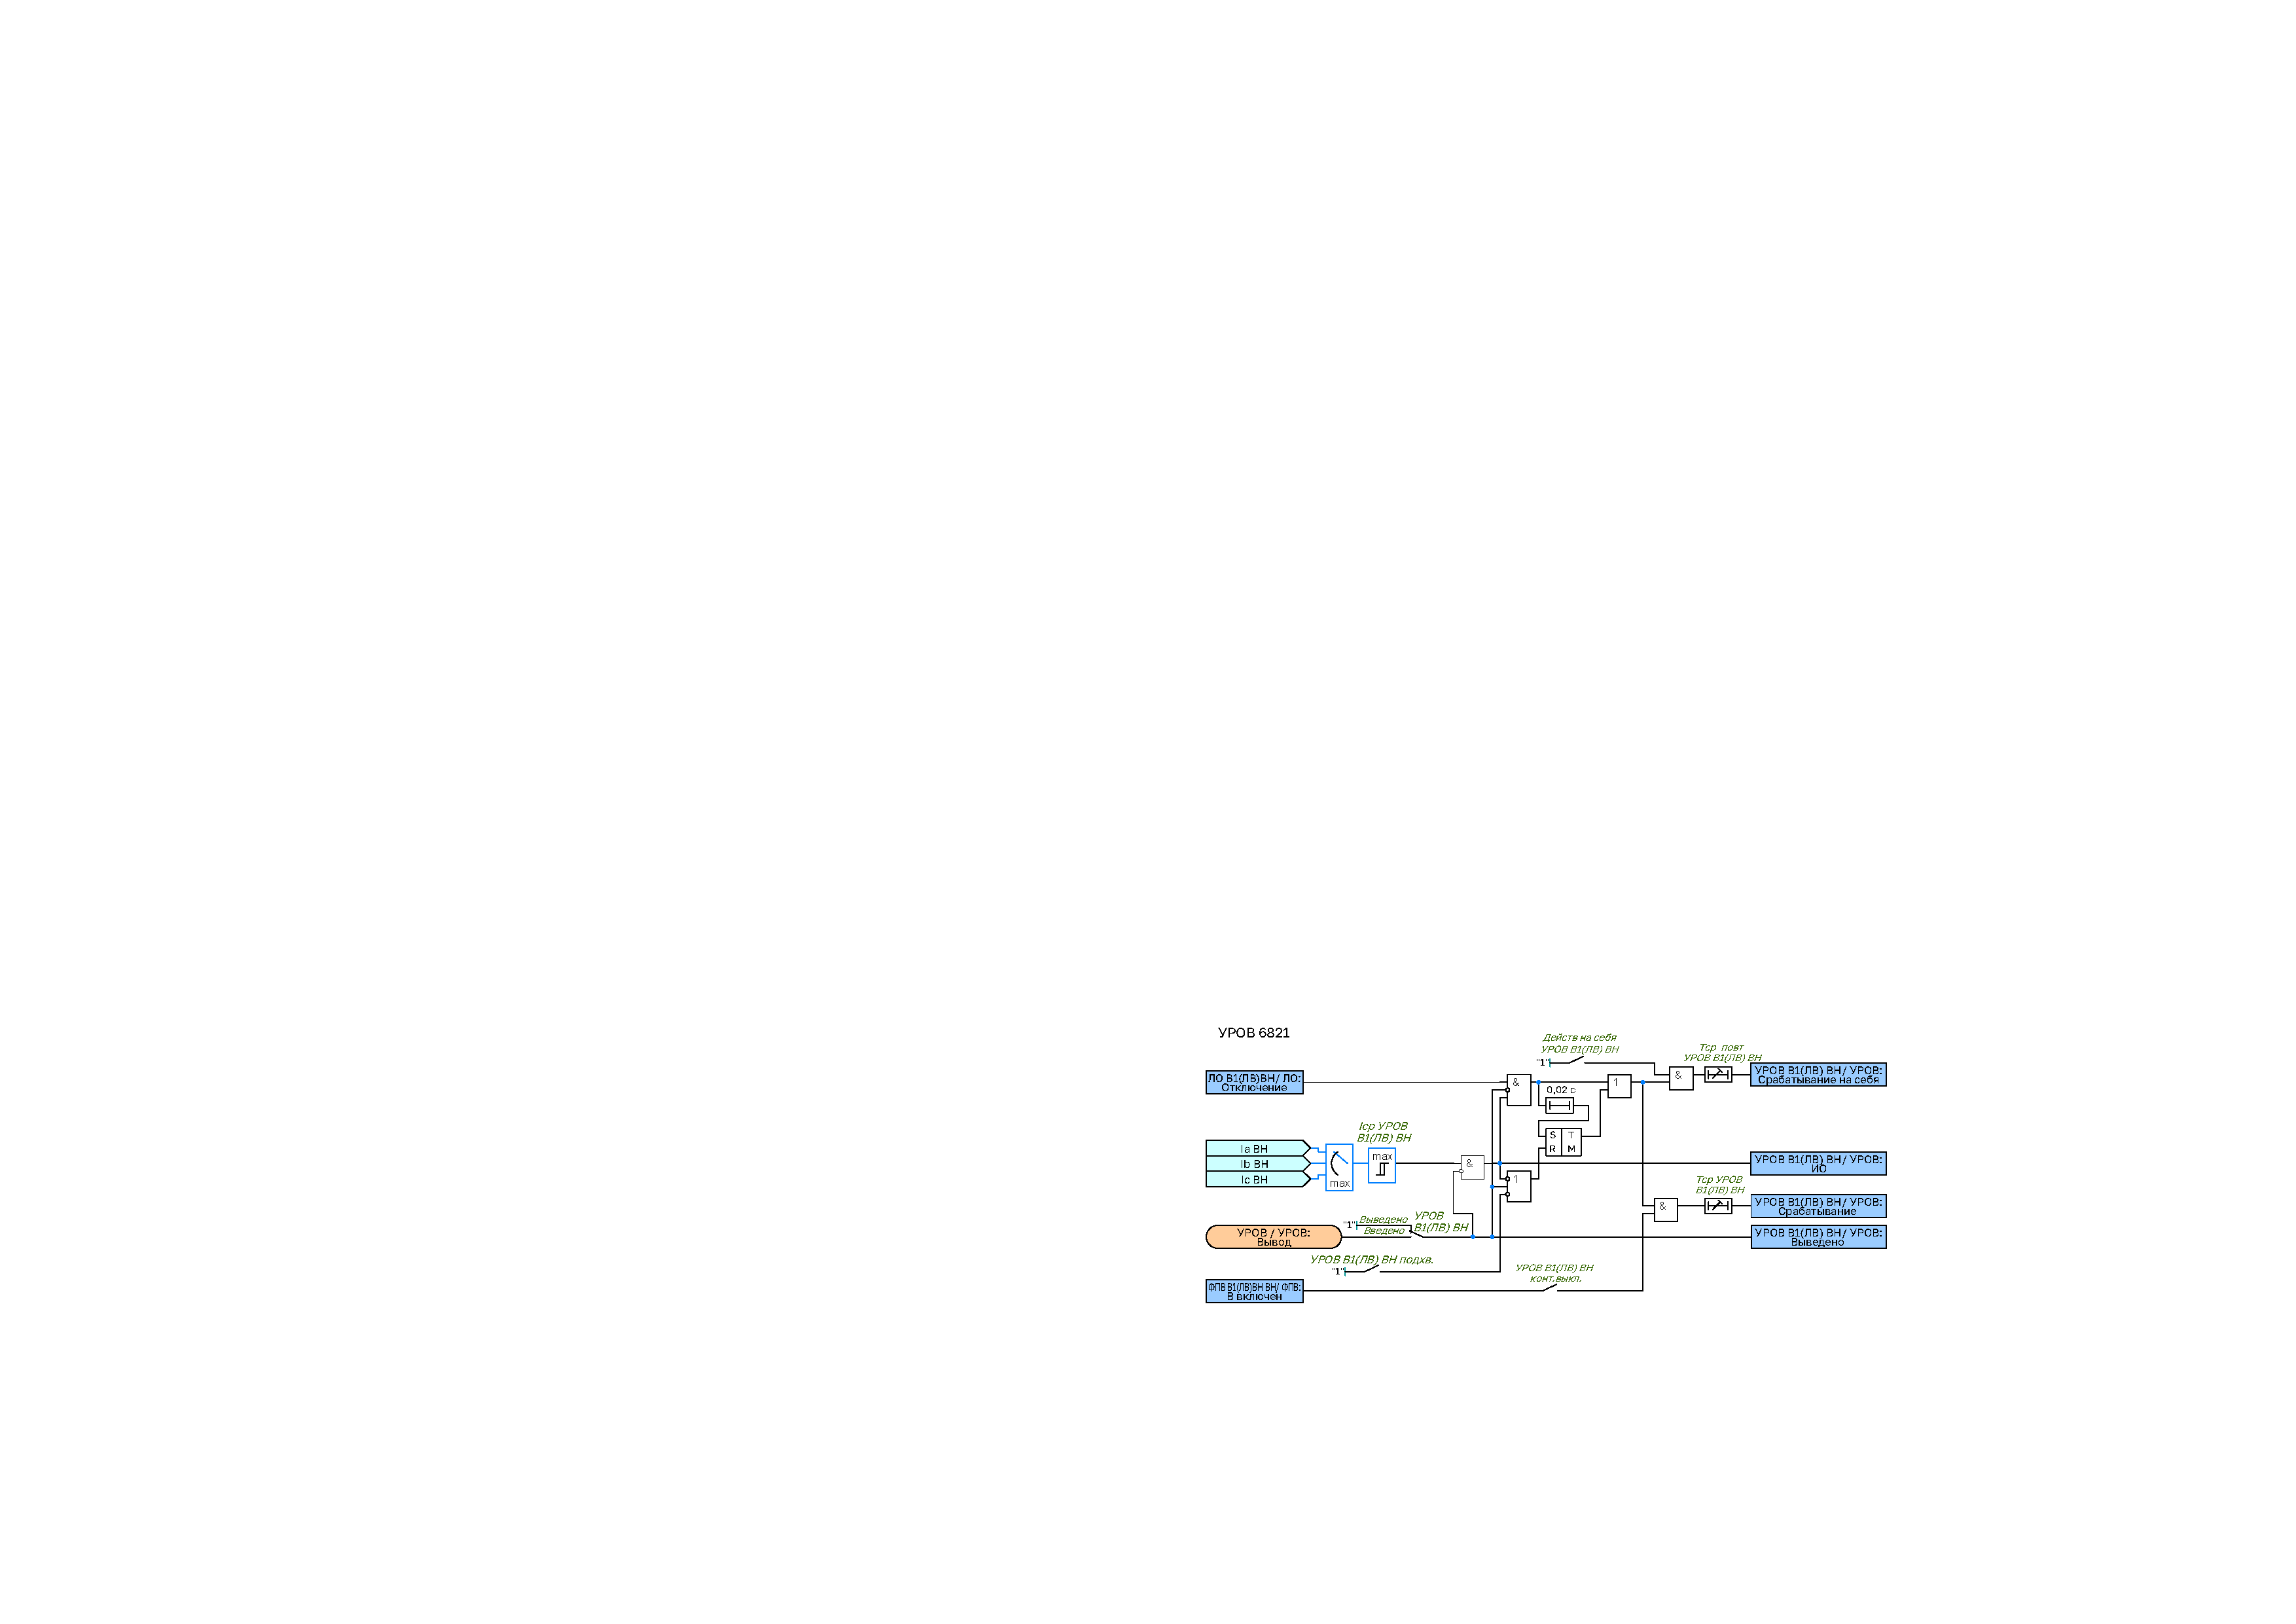
\includegraphics[width=1\textwidth,height=1\textheight,keepaspectratio]{img26.pdf}
\captionof{figure}{Функциональная схема логики УРОВ ВН}\label{pic:UROV}
\end{figure}

\end{enumerate}
\color{unidarkgreen}{\subsection{Пусковой орган устройства резервирования при отказе выключателя при повреждениях на стороне НН}}
\color{black}

\begin{enumerate}[label=\arabic{section}.\arabic{subsection}.\arabic*,  align=left, labelsep=4pt, leftmargin=0pt, itemindent=57pt]

\item
Пусковой орган устройства резервирования при отказе выключателя при повреждениях на стороне НН (ПО УРОВ НН) предназначен для пуска УРОВ выключателей сторон ВН и СН автотрансформатора при недостаточной чувствительности своих измерительных органов по току при повреждениях на стороне НН автотрансформатора.

\item
Логика работы ПО УРОВ НН выполнена с контролем протекания тока по стороне НН автотрансформатора. Значение по току срабатывания задается параметром \textbf{«Iср УРОВ В»}. Функция УРОВ действует с регулируемой задержкой по времени \textbf{«Тср повт. УРОВ»} на повторное отключение своего выключателя, с задержкой \textbf{«Тср УРОВ»} на отключение смежных выключателей.

\item
Предусмотрен подхват по току, включение которого производится программной накладкой \textbf{«ПО УРОВ подхв.»}.

\item
Алгоритм работы ПО УРОВ НН приведен на рисунке \ref{pic:UROVNN}. Уставки ПО УРОВ НН приведены в таблице \ref{app_set:urovnn}.

\begin{figure}[H]
\centering
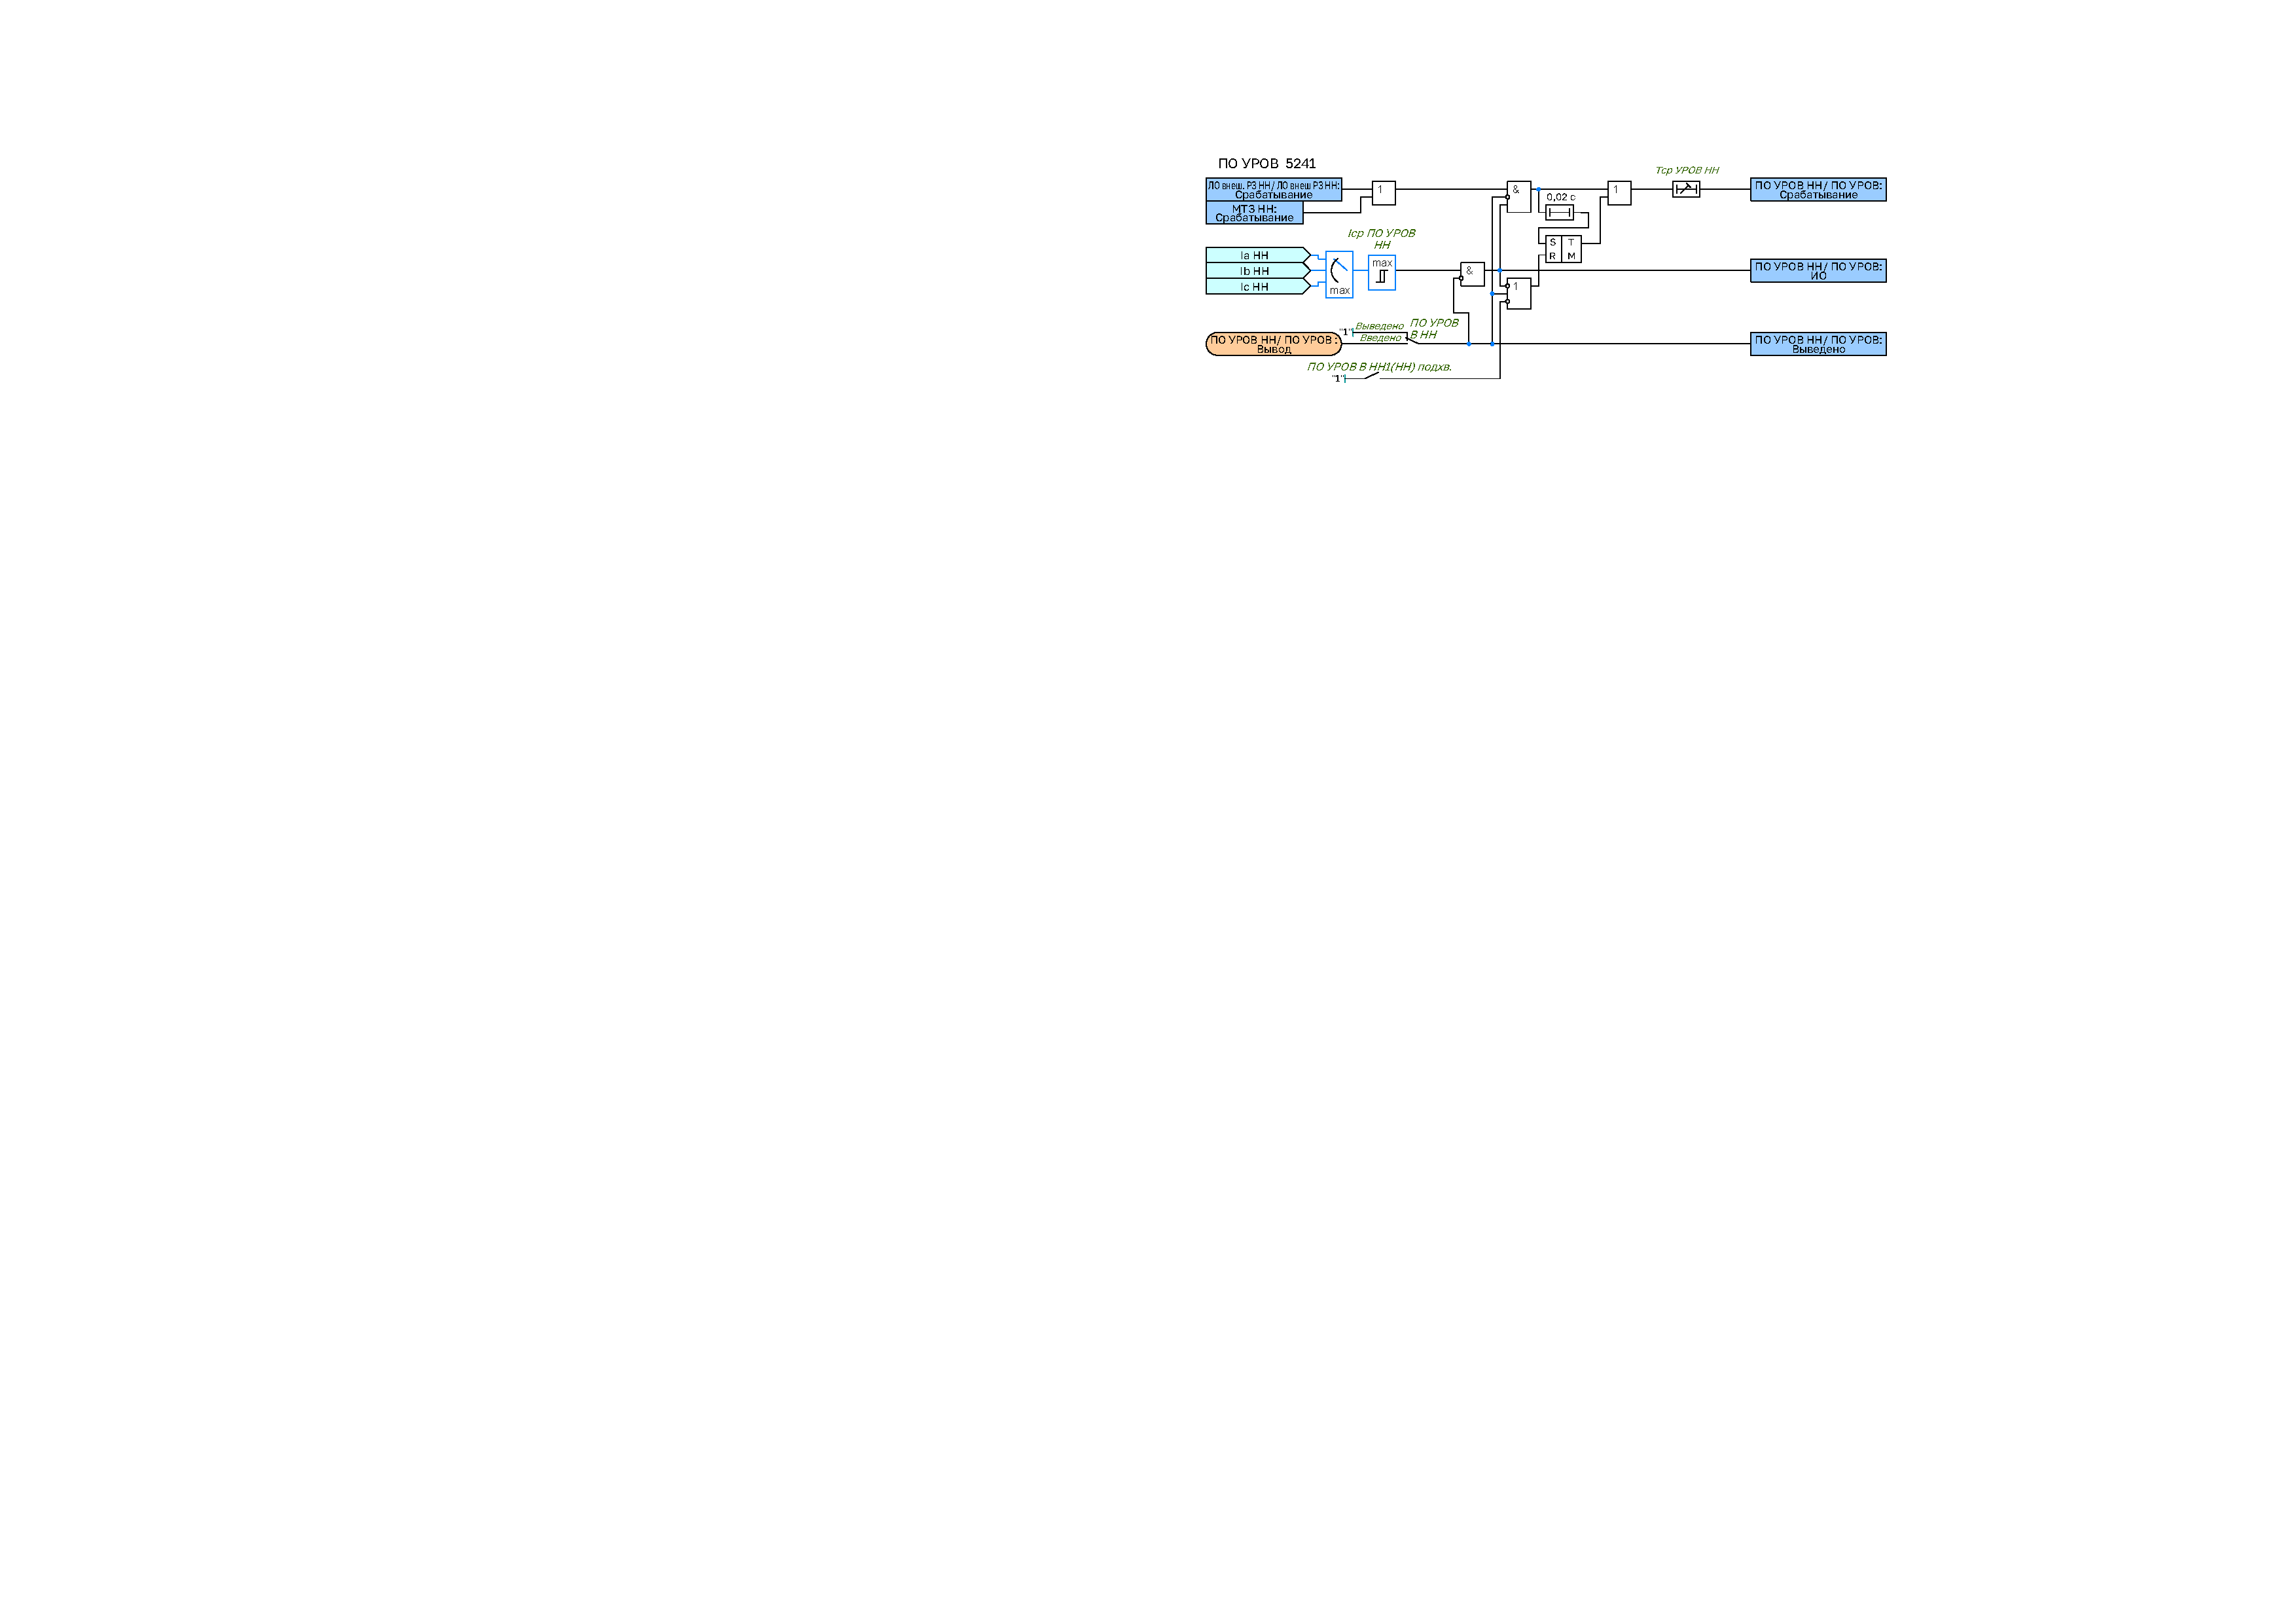
\includegraphics[width=1\textwidth,height=1\textheight,keepaspectratio]{img27.pdf}
\captionof{figure}{Функциональная схема логики ПО УРОВ НН}\label{pic:UROVNN}
\end{figure}



\end{enumerate}
\color{unidarkgreen}{\subsection{Управление выключателем}}
\color{black}

\begin{enumerate}[label=\arabic{section}.\arabic{subsection}.\arabic{subsubsection}.\arabic*,  align=left, labelsep=4pt, leftmargin=0pt, itemindent=57pt]

\item
Функциональный блок управления выключателем предназначен для формирования сигнала на включение силового выключателя. 

\item
В случае присоединения автотрансформатора к шинам ВН и СН через свой выключатель для каждого из них можно задействовать свою логику управления выключателем. Далее приведено описание логики управления выключателем В ВН, логика управления выключателем В СН аналогична.

\item
Команда на включение выключателя \textit{«Включить В1»} формируется:
\begin{itemize}
\item от команды оперативного включения выключателя (сигнал \textit{«РКВ В1(ЛВ)ВН»});
\item при срабатывании АПВ (сигнал \textit{«Ср. АПВ В1(ЛВ)ВН»}); 
\item от внешнего сигнала включения \textit{«Внеш. вкл. В1(ЛВ)ВН»}.
\end{itemize}

\item
Оперативное включение выключателя осуществляется с контролем наличия разрешающего сигнала от функции контроля синхронизма и напряжений (КСН). Максимальное время, в течение которого продолжается ожидание условий оперативного включения, регулируется уставкой \textbf{«Tожид усл. опер. вкл. В1»}. По истечению данной выдержки времени команда оперативного включения сбрасывается. Выдержка времени на возврат \textbf{«Тпрод опер. вкл. В1»} задает время продления сигнала оперативного включения.

\item
При необходимости может быть введен подхват команды на включение от токового реле, установленного в цепи ЭМВ, в этом случае сигнал на включение удерживается в сработанном состоянии до исчезновения тока через ЭМВ (пока блок-контакты выключателя не разорвут цепь включения). Ввод осуществляется программным ключом \textbf{«Подхват вкл. В1 от РТ ЭМВ»}. 

\item
Предусмотрена возможность блокировки многократных включений на КЗ. Если при наличии сигнала включения будет протекать ток по электромагнитам отключения (что соответствует включению на КЗ), то сигнал \textit{«Включить В1»} заблокируется, пока не пропадут сигналы включения (от АПВ или оперативного включения). Блокировка вводится программным ключом \textbf{«Блок. от многокр. вкл. на КЗ В1»}.

\item
При наличии сигнала \textit{«Блок. включения В1»}, формируемого функциональным блоком контроля силового выключателя, включение выключателя блокируется.

\item
Алгоритм работы функции управления выключателем стороны ВН приведен на рисунке \ref{pic:OPQ}, алгоритм работы функции управления выключателем стороны СН аналогичный. Уставки УВ ВН приведены в таблице \ref{app_set:uvvn}. Уставки УВ СН приведены в таблице \ref{app_set:uvsn}.

\vspace{2mm}
\begin{figure}[H]
\centering
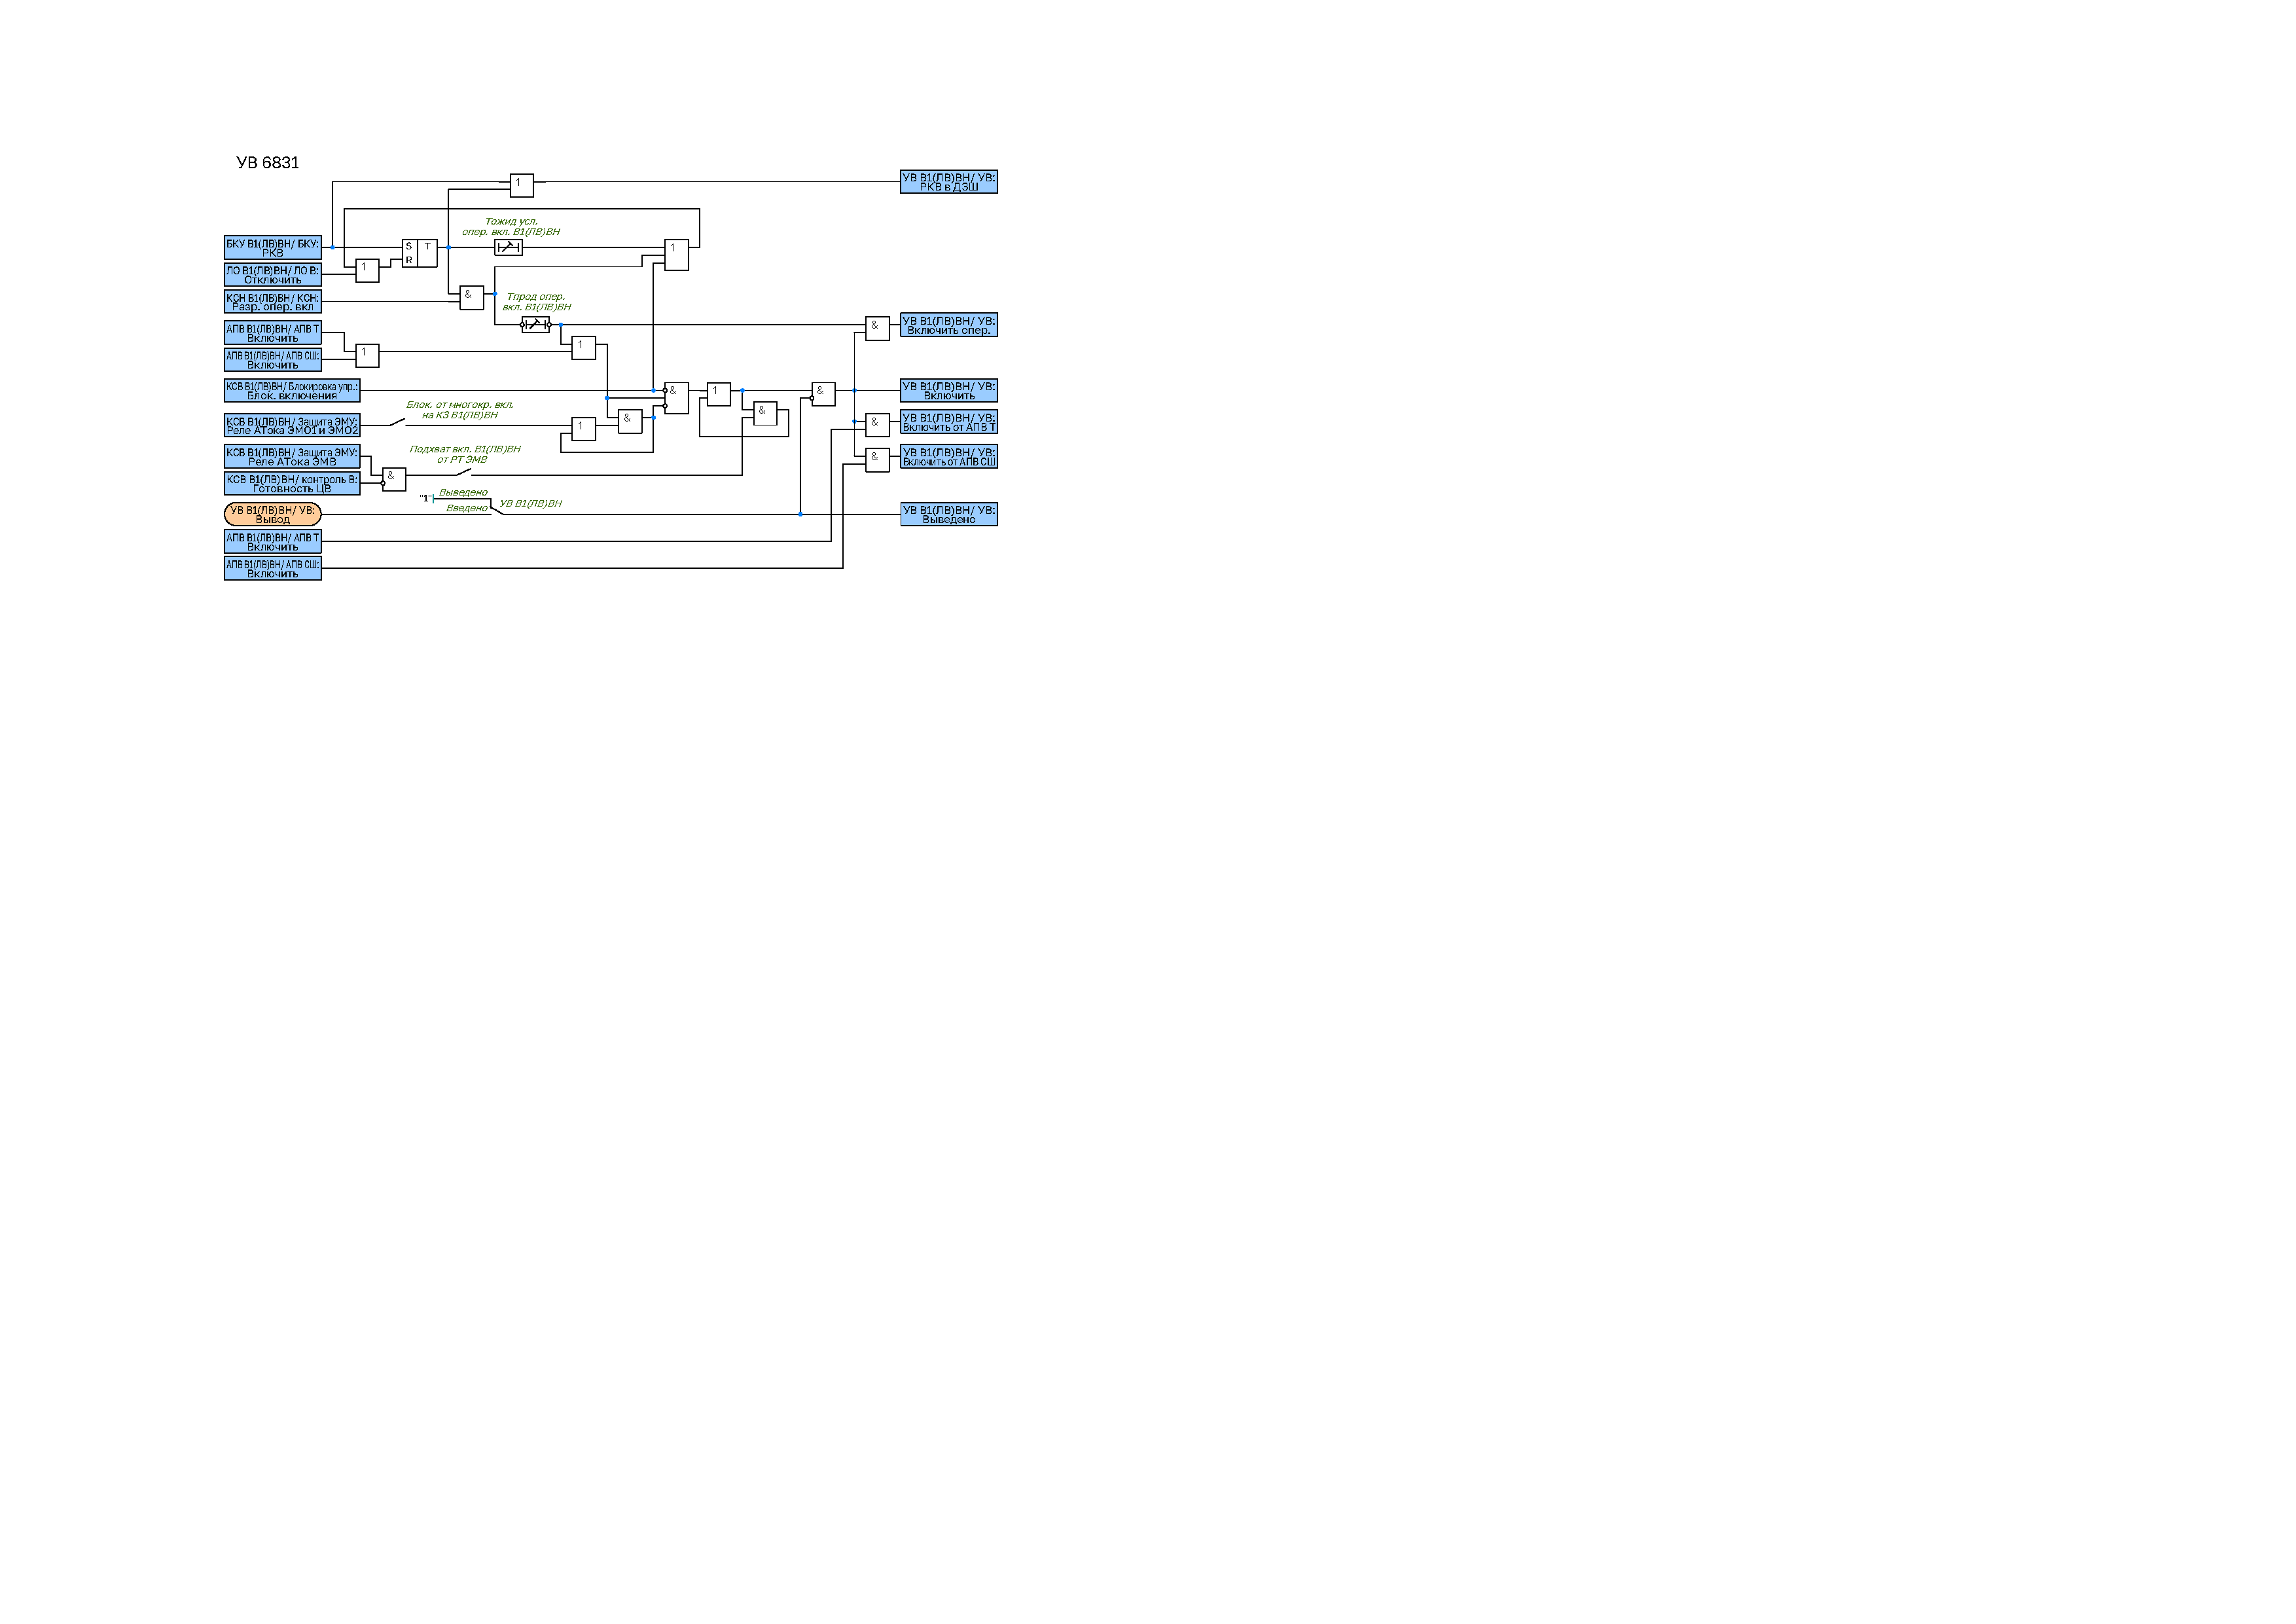
\includegraphics[width=1\textwidth,height=1\textheight,keepaspectratio]{img28.pdf}
\captionof{figure}{Функциональная схема логики управления выключателем стороны ВН}\label{pic:OPQ}
\end{figure}

\end{enumerate}
\color{unidarkgreen}{\subsection{Блок команд управления}}
\color{black}

\begin{enumerate}[label=\arabic{section}.\arabic{subsection}.\arabic*,  align=left, labelsep=4pt, leftmargin=0pt, itemindent=57pt]

\item
Функциональный блок команд управления выключателем предназначен для контроля формируемого сигнала на включение или отключение силового выключателя при оперативном управлении.

\item
Алгоритм работы логики блока команд управления выключателя В1(ЛВ) ВН приведен на рисунке \ref{pic:LO_Q1_NN}. Алгоритм работы логики блока команд управления выключателя В1(ЛВ) СН выполнен аналогично. Уставки БКУ выключателей стороны ВН и СН приведены в таблицах \ref{app_set:bkuvn}, \ref{app_set:bkusn}.

\begin{figure}[H]
\centering
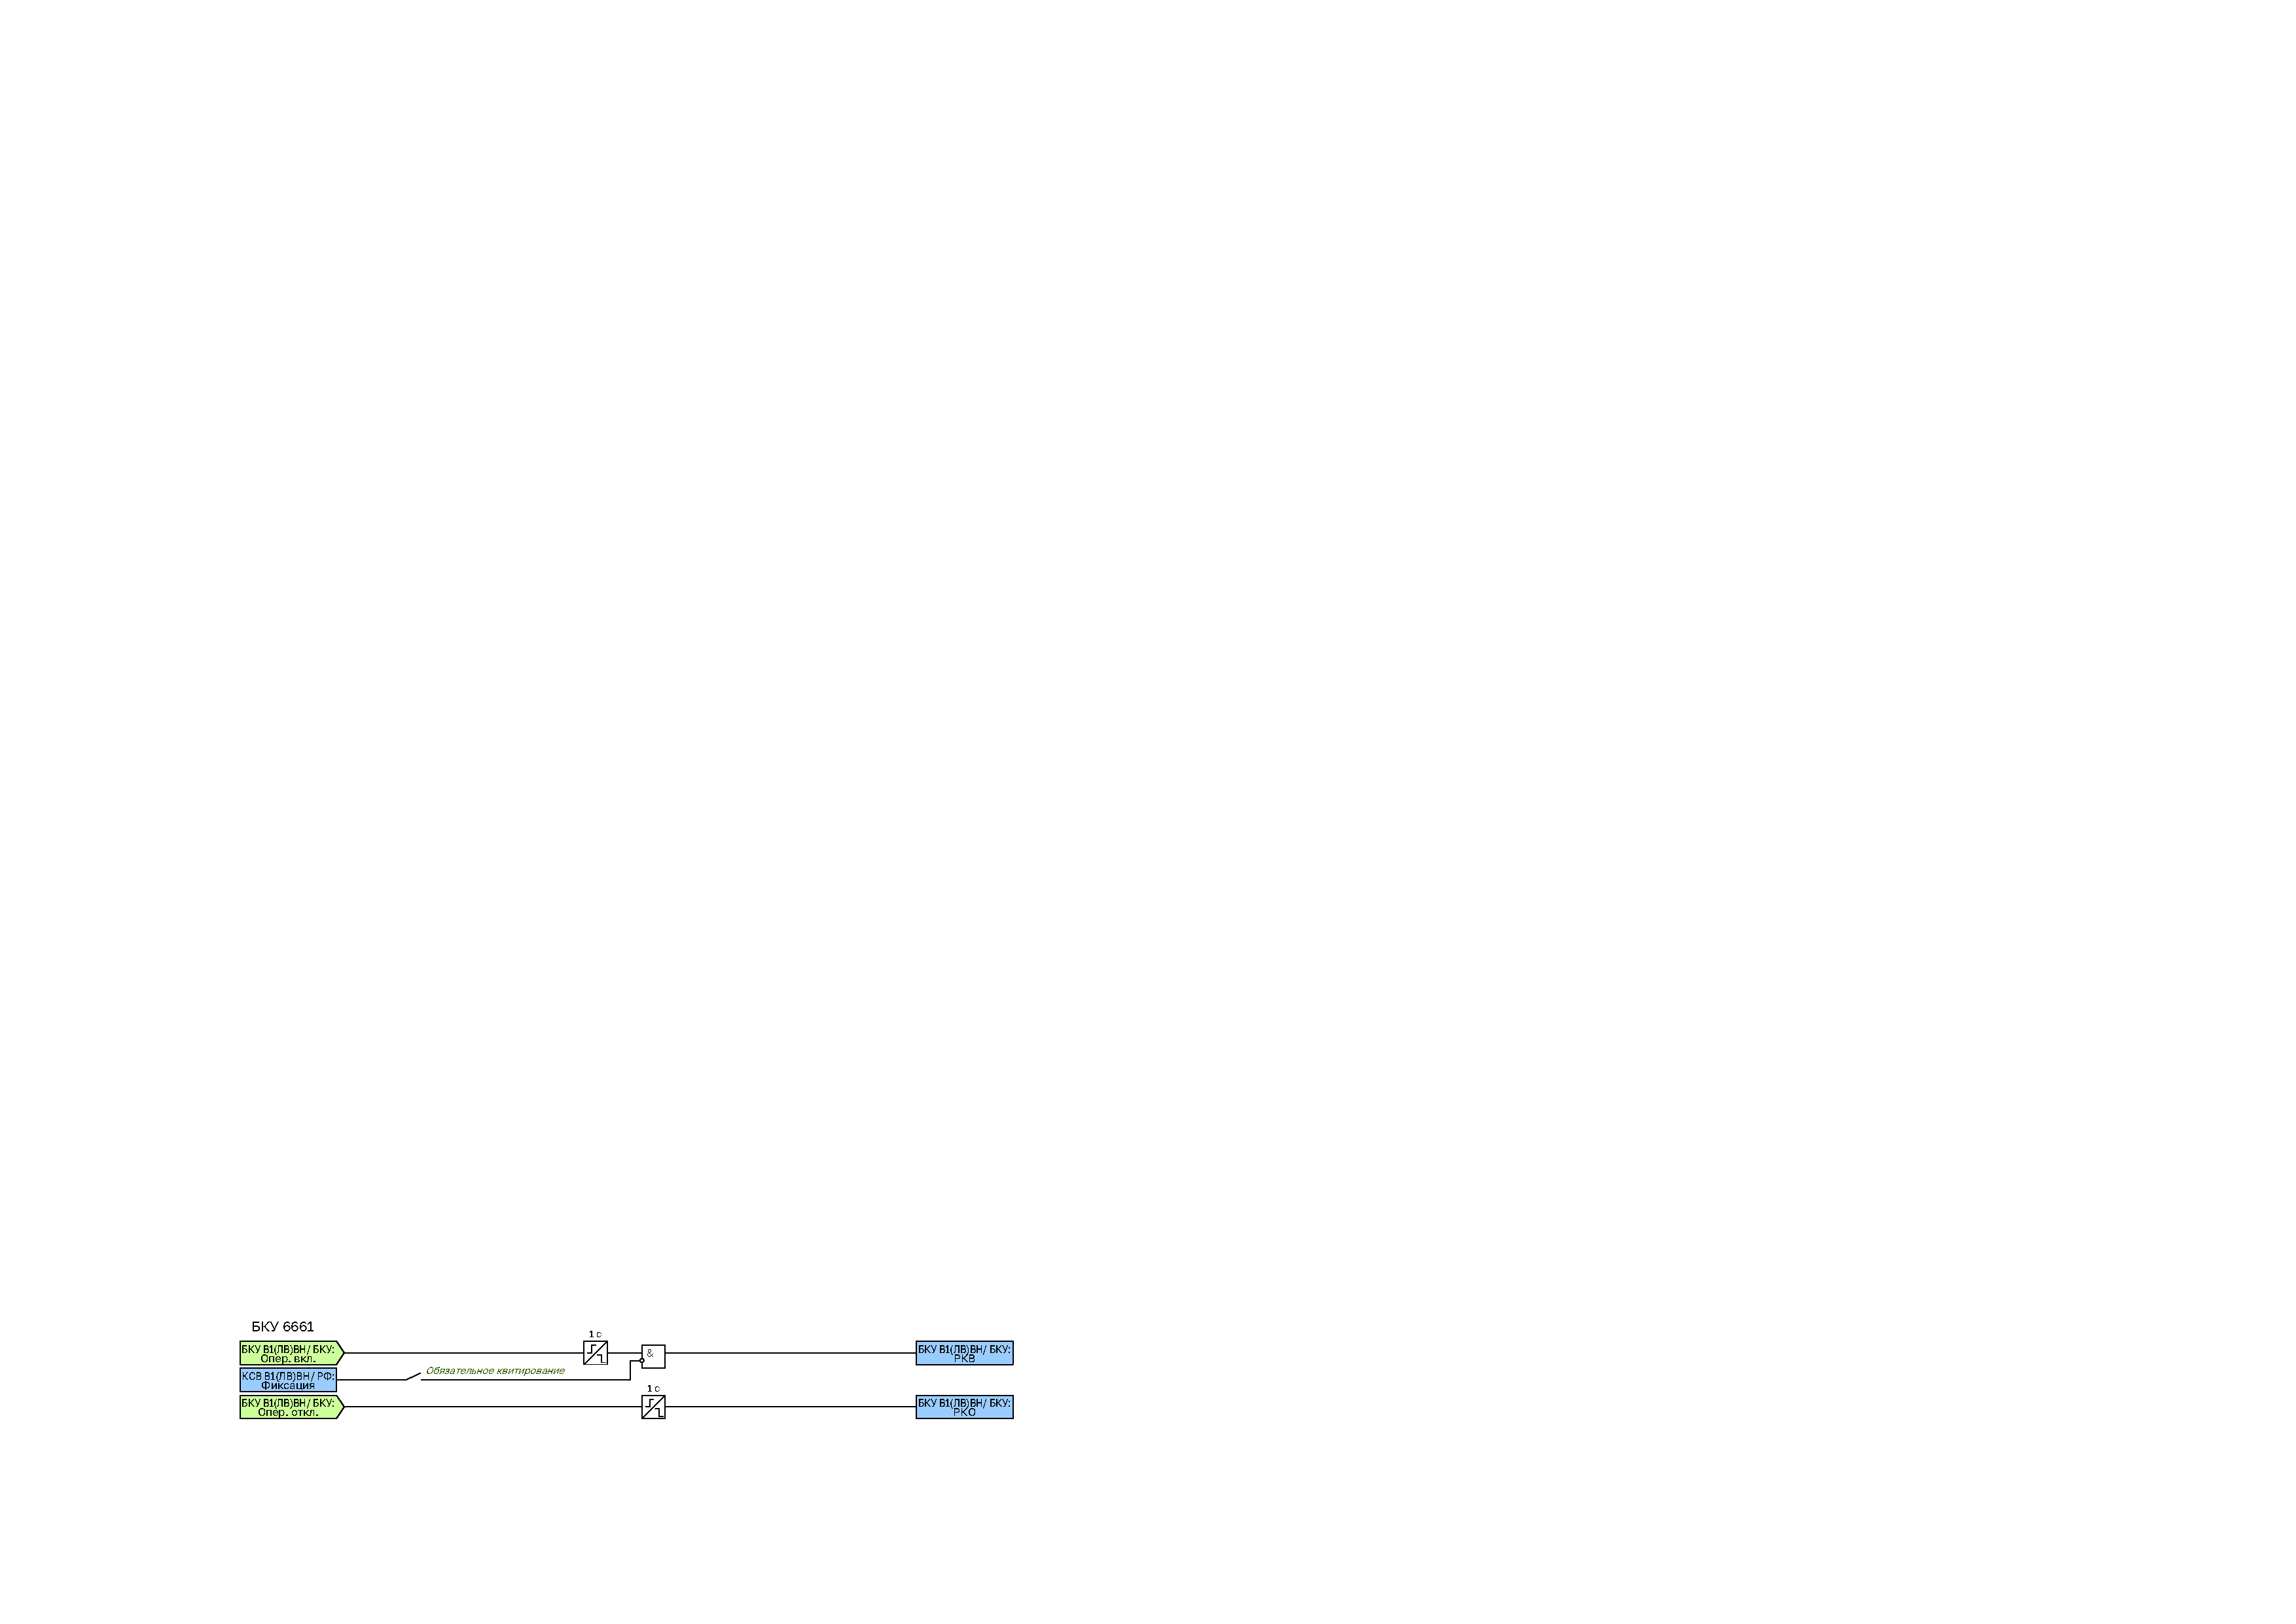
\includegraphics[width=1\textwidth,height=1\textheight,keepaspectratio]{img29.pdf}
\captionof{figure}{Функциональная схема логики блока команд управления В1(ЛВ) ВН}\label{pic:BKU}
\end{figure}


\end{enumerate}\color{unidarkgreen}{\subsection{Контроль синхронизма и напряжений}}
\color{black}

\begin{enumerate}[label=\arabic{section}.\arabic{subsection}.\arabic{subsubsection}.\arabic*,  align=left, labelsep=4pt, leftmargin=0pt, itemindent=57pt]

\item
Функциональный блок контроля синхронизма и напряжений (КСН) предназначен для формирования разрешающих сигналов, соответствующих условиям включения, для АПВ, оперативного включения. Функциональный блок КСН В1(ЛВ)СН аналогичен КСН В1(ЛВ)ВН.

\item
Основные режимы включения и контролируемые для них условия приведены в таблице \ref{desc:tbl1}. Режимы включения с контролем синхронизма (КС) и с улавливанием синхронизма (УС) вводятся соответствующими программными ключами \textbf{«КС В1(ЛВ) ВН»} и \textbf{«УС В1(ЛВ) ВН»}.

\item
Если разность частот напряжений шин и трансформатора не превышает уставку \textbf{«df макс КС»}, то разрешается включение с контролем синхронизма. Для режима включения с КС также контролируется:
\begin{itemize}
\item наличие напряжения на обоих энергообъектах (шины и трансформатор);
\item разность напряжений шин и трансформатора, не превышающая по модулю значения заданной уставки;
\item разность фаз напряжений шин и трансформатора, не превышающая по модулю значения заданной уставки.
\end{itemize}

\item
При выводе программного ключа \textbf{«КС В1(ЛВ) ВН»} включение разрешается без контроля частоты, а только по уровню напряжений и разности их фаз.

\item
Если разность частот превышает уставку \textbf{«df макс КС»}, но не выходит за пределы уставки \textbf{«df пред. доп.»}, то разрешается включение с улавливанием синхронизма. Сигнал включения с улавливанием синхронизма формируется с опережением на время включения выключателя. Режим включения с УС можно вывести программным ключом \textbf{«УС В1(ЛВ) ВН»}.

\item
Наличие или отсутствие напряжения на трансформатор контролируется измерительными органами максимального и минимального напряжения, пороги срабатывания которых задаются уставками \textbf{«Uнал Т В1(ЛВ) ВН»} и \textbf{«Uотс Т В1(ЛВ) ВН»} соответственно. Пороги срабатывания измерительных органов для контроля напряжения на энергообъекте Ш (шины) задаются уставками \textbf{«Uнал Ш В1(ЛВ) ВН»} и \textbf{«Uотс Ш В1(ЛВ) ВН»}.

\small
\begin{longtable}{|>{\centering\arraybackslash}m{5.3cm}|>{\centering\arraybackslash}m{11.6cm}|}
\caption{Условия включения\hfill\vspace{-0.5\baselineskip}}\label{desc:tbl1}\\
\hline
\rowcolor{gray!30}
Режим включения & Условия включения \\
\hline
\endfirsthead

\caption*{\hspace{3pt}\emph{Продолжение таблицы \ref{desc:tbl1}}\hfill\ }\vspace{-0.5\baselineskip} \\
\hline
\rowcolor{gray!30}
Режим включения & Условия включения \\
\hline
\endhead

ОНАТ+ННШ &   
			\begin{itemize}
			\vspace{3pt}
			\item $ \textrm{U}_\textrm{T} $ меньше уставки \textbf{«Uотс АТ В1(ЛВ) ВН»};
			\item $ \textrm{U}_\textrm{Ш} $ больше уставки \textbf{«Uнал Ш В1(ЛВ) ВН»}.
			\vspace{3pt}
			\end{itemize} \\
\hline
ННШ+ННАТ & 
			\begin{itemize}
			\vspace{3pt}
			\item $ \textrm{U}_\textrm{T} $ больше уставки \textbf{«Uнал АТ В1(ЛВ) ВН»};
			\item $ \textrm{U}_\textrm{Ш} $ меньше уставки \textbf{«Uотс Ш В1(ЛВ) ВН»}.
			\vspace{3pt}
			\end{itemize} \\
\hline
КС(УС)	&
			\vspace{3pt}
			
			\begin{itemize}
			\item[] \noindent 1) Включение контролем синхронизма:
			\item $ \textrm{U}_\textrm{T} $ больше уставки \textbf{«Uнал АТ В1(ЛВ) ВН»};
			\item $ \textrm{U}_\textrm{Ш} $ больше уставки \textbf{«Uнал Ш В1(ЛВ) ВН»};
			\item разность напряжений трансформатора и шин не превышает по модулю значения заданной уставки \textbf{«dU макс КС(УС)»};
			\item разность фаз напряжений трансформатора и шин не превышает по модулю значения заданной уставки \textbf{«dФ макс КС»};
			\item разность частот напряжений трансформатора и шин не превышает значения заданной уставки \textbf{«df макс КС»};
			\end{itemize}
			
			\begin{itemize}
			\item[] \noindent  2) Включение с улавливанием синхронизма:
			\item $ \textrm{U}_\textrm{T} $ больше уставки \textbf{«Uнал АТ В1(ЛВ) ВН»};
			\item $ \textrm{U}_\textrm{Ш} $ больше уставки \textbf{«Uнал Ш В1(ЛВ) ВН»};
			\item разность напряжений трансформатор и шин не превышает по модулю значения заданной уставки \textbf{«dU макс КС(УС)»};
			\item разность частот напряжений трансформатора и шин превышает значение уставки \textbf{«df макс КС»};
			\item разность частот напряжений трансформатора и шин не превышает значения заданной уставки \textbf{«df пред. доп.»};
			\item за время \textbf{«Т опер. вкл. В1(ЛВ) ВН»} с момента подачи сигнала на включение выключателя расхождение углов между векторами напряжений на трансформаторе и шине превысит 10º.
			\vspace{3pt}
			\end{itemize} \\
\hline

\end{longtable}
\normalsize	

\item
Сигнал разрешения АПВ автотрансформатор \textit{«Разр. АПВат В1(ЛВ) ВН»} формируется при выполнении условий включения в режимах ОНАТ+ННШ, КС или УС.

\item
Сигнал разрешения АПВ шин \textit{«Разр. АПВш В1(ЛВ) ВН»} формируется при выполнении условий включения в режимах ОНШ+ННАТ, КС или УС. 

\item
Сигнал разрешения оперативного включения \textit{«Разр. опер. вкл. В1(ЛВ) ВН»} может формироваться от внутренней логики КСН или от внешнего сигнала в зависимости от положения программного переключателя \textbf{«Контр. опер. вкл. В1(ЛВ) ВН»}.

\item
В положении \textit{«Внутр.»} оперативное включение разрешается при выполнении условий включения в режимах ОНАТ+ННШ (при опробовании автотрансформатора), ОНШ+ННАТ (при опробовании шин), КС или УС (при замыкании в транзит). Также предусмотрена возможность оперативного включения с контролем отсутствия напряжения на шинах или на автотрансформатор при введенном программном ключе \textbf{«Опер. вкл. В1(ЛВ) ВН с КОН»}. При отсутствии внешнего сигнала \textit{«Опер. вкл. с КС(УС) В1(ЛВ) ВН»} оперативное включение может выполняться без контроля напряжений и условий синхронизма.

\item
В положении \textit{«Внеш.»} оперативное включение разрешается при наличии внешнего сигнала \textit{«Внеш. сигнал КС(УС) В1(ЛВ) ВН»}.

\item
Сигнал разрешения полуавтоматического включения \textit{«Разр. ПАВ В1(ЛВ) ВН»} формируется при выполнении условий включения в режимах КС или УС.

\item
Алгоритм работы КСН ВН приведен на рисунке \ref{pic:KSN}, алгоритм работы КСН СН выполнен аналогично. Уставки КСН ВН приведены в таблице \ref{app_set:ksnvn}. Уставки КСН СН приведены в таблице \ref{app_set:ksnsn}.

\begin{figure}[H]
\centering
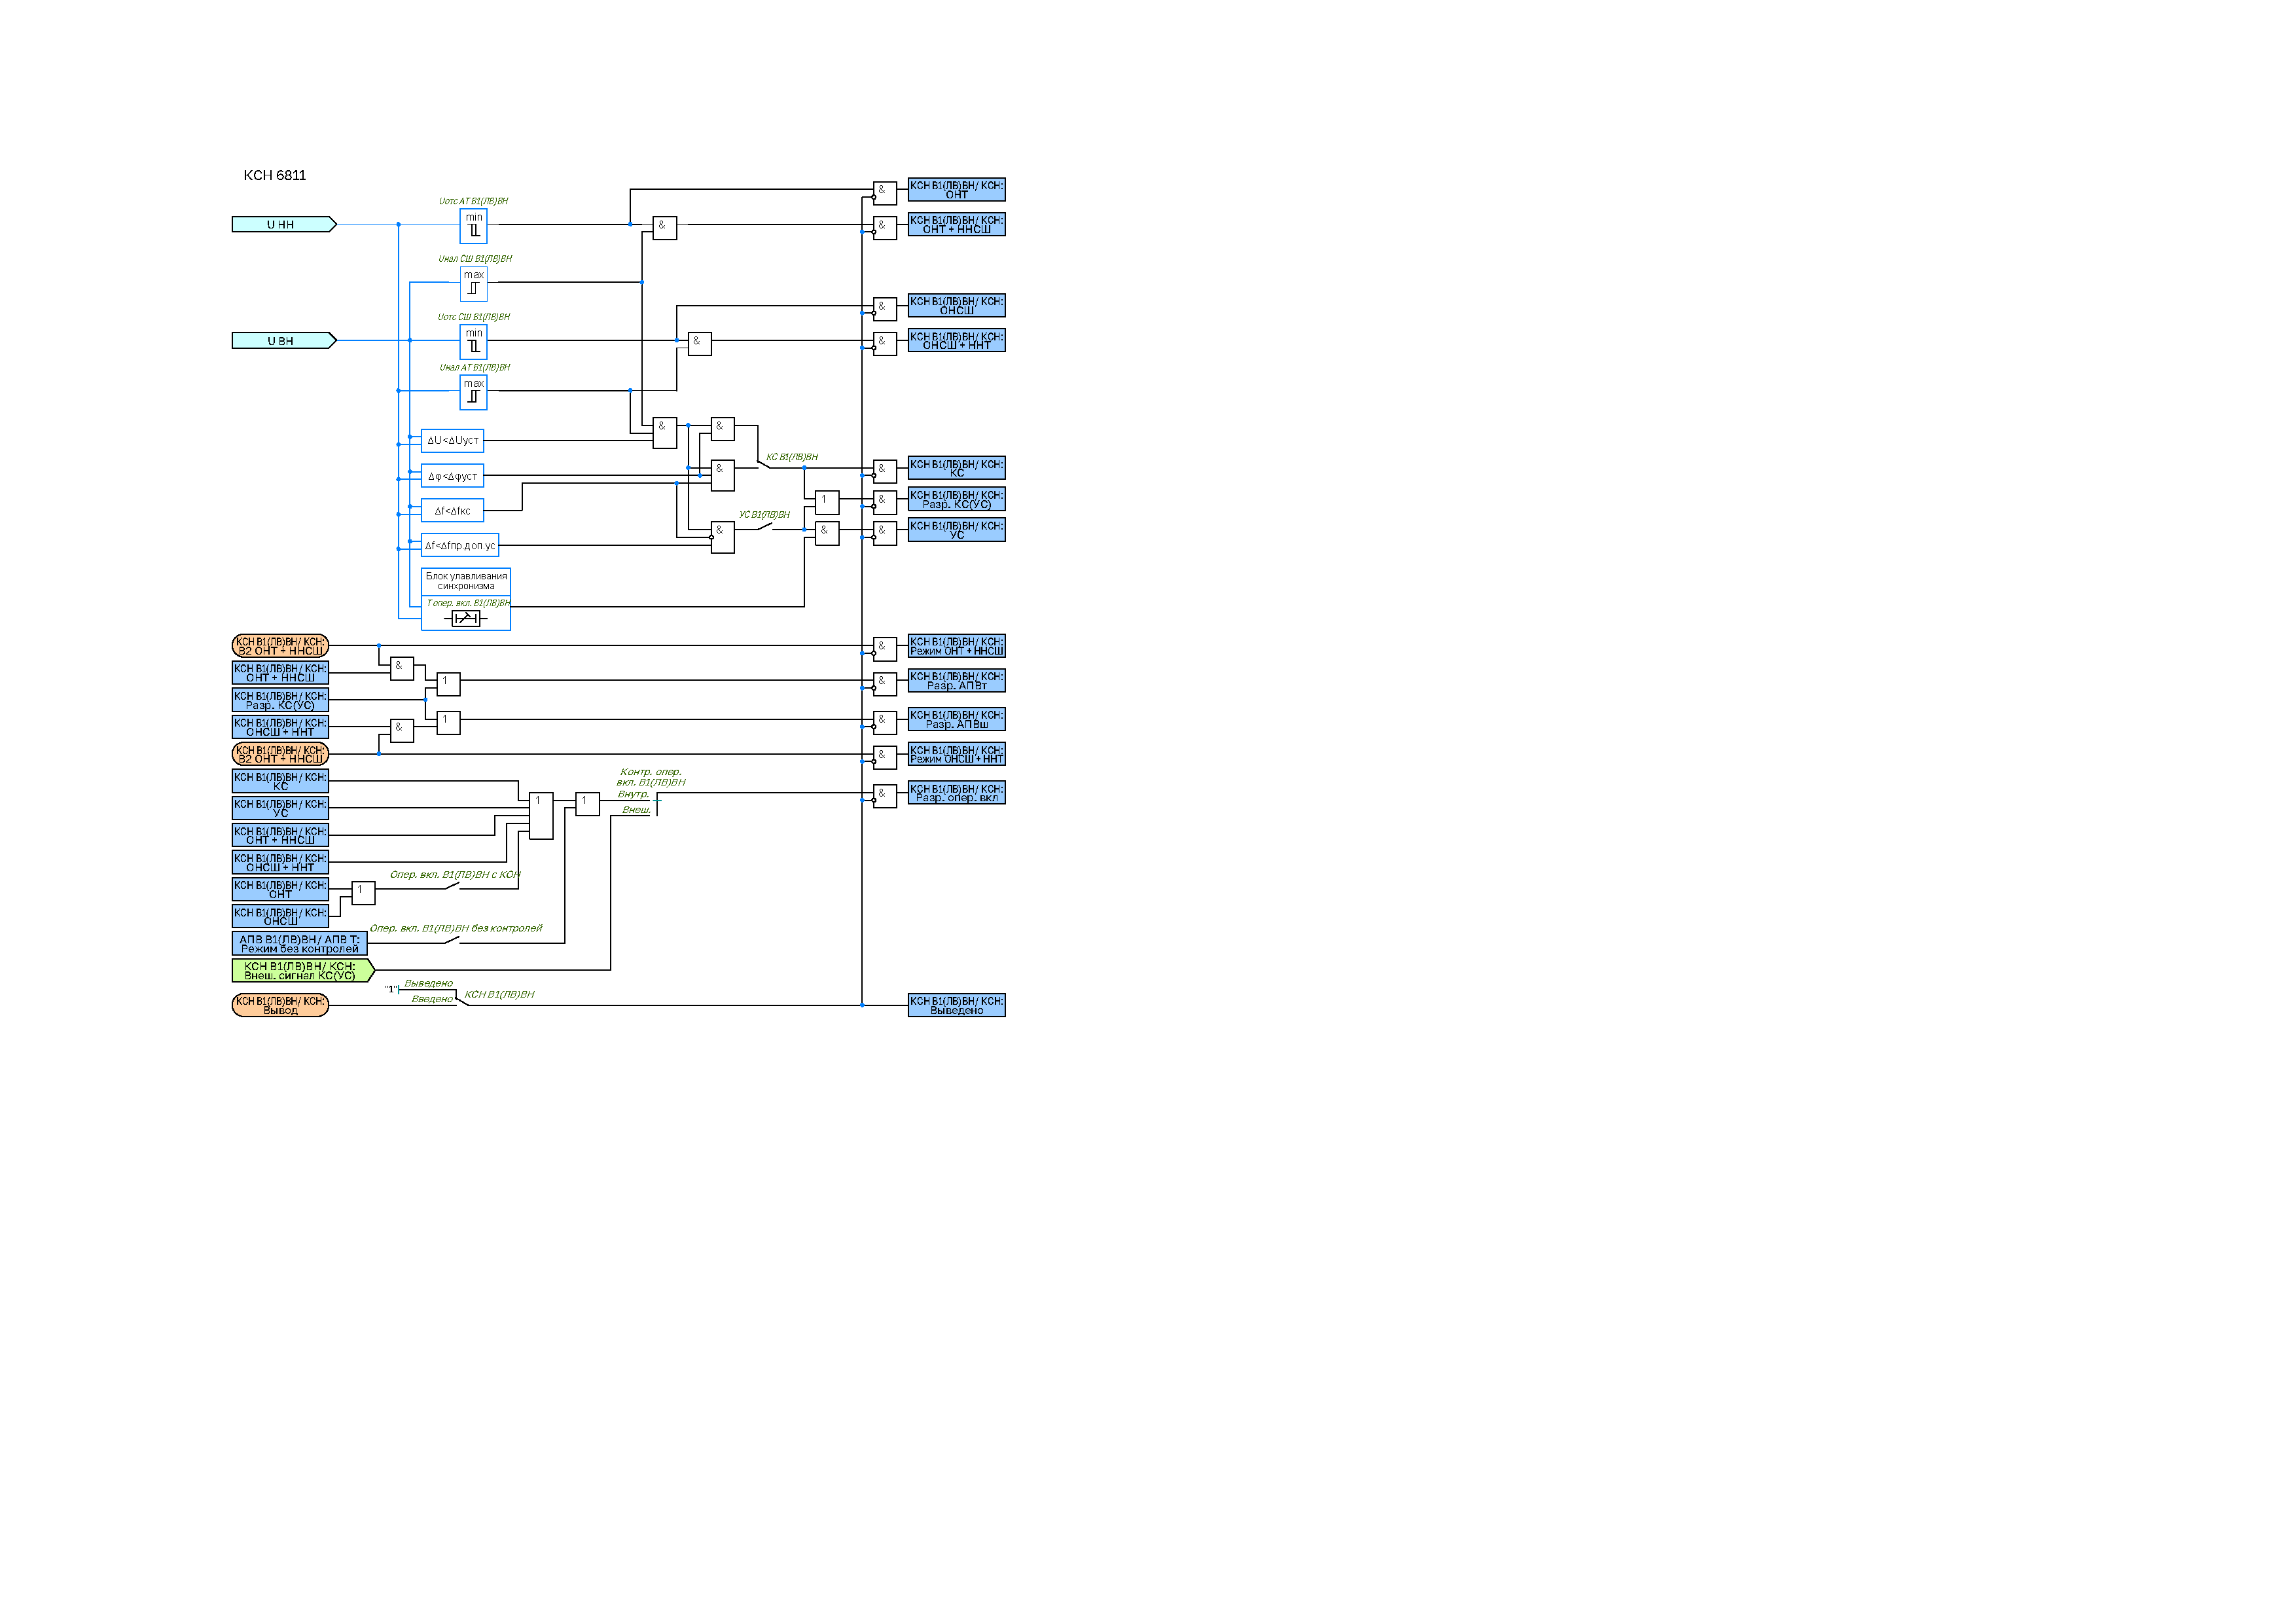
\includegraphics[width=0.8\textwidth,height=0.8\textheight,keepaspectratio]{img30.pdf}
\captionof{figure}{Функциональная схема логики КСН В1(ЛВ) ВН}\label{pic:KSN}
\end{figure}

\end{enumerate}\color{unidarkgreen}{\subsection{Автоматическое повторное включение}}
\color{black}

\begin{enumerate}[label=\arabic{section}.\arabic{subsection}.\arabic*,  align=left, labelsep=4pt, leftmargin=0pt, itemindent=57pt]

\item
Автоматическое повторное включение (АПВ) предназначено для быстрого восстановления первоначального состояния электрической сети после аварийного отключения путём автоматического включения выключателя.

\item
Выбор действующих режимов АПВ для выключателя В1(ЛВ) ВН реализуется тремя входными сигналами ФСУ:
\begin{itemize}
\item \textit{«АПВ В1(ЛВ) ВН ОНАТ + ННШ»} (включение с контролем отсутствия напряжения на трансформаторе и наличия напряжения на шинах) – АПВ автотрансформатора;
\item \textit{«АПВ В1(ЛВ) ВН ОНШ» + ННАТ»} (включение с контролем отсутствия напряжения на шинах и наличия напряжения на автрансформаторе) – АПВ шин;
\item \textit{«АПВ В1(ЛВ) ВН без контролей»} (включение без контроля напряжений).
\end{itemize}

\item
Возможные режимы АПВ приведены в таблице \ref{desc:apvtbl1}. Уставки АПВ ВН приведены в таблице \ref{app_set:apvvn}. Уставки АПВ СН приведены в таблице \ref{app_set:apvsn}.

\small
\renewcommand{\arraystretch}{1}
\setlength{\extrarowheight}{2pt}

\begin{longtable}{|>{\centering\arraybackslash}m{5.2cm}|>{\centering\arraybackslash}m{3.6cm}|>{\centering\arraybackslash}m{3.6cm}|>{\centering\arraybackslash}m{3.6cm}|}
\caption{Условия включения\hfill\vspace{-0.5\baselineskip}}\label{desc:apvtbl1}\\
\hline
\rowcolor{gray!30}
& \multicolumn{3}{c|}{Входные сигналы ФСУ} \\
\hhline{>{\arrayrulecolor{gray!30}}->{\arrayrulecolor{black}}|-|-|-|}
\rowcolor{gray!30}
\raisebox{3pt}{\makecell[c]{Режим АПВ}} & 
\makecell[c]{АПВ В1(ЛВ) ВН \\ ОНАТ+ННШ} & 
\makecell[c]{АПВ В1(ЛВ) ВН \\ ОНШ+ННАТ} & 
\makecell[c]{АПВ В1(ЛВ) ВН \\ без контролей} \\
\hline
\endfirsthead

\caption*{\hspace{3pt}\emph{Продолжение таблицы \ref{desc:apvtbl1}}\hfill\ }\vspace{-0.5\baselineskip} \\
\hline
\rowcolor{gray!30}
& \multicolumn{3}{c|}{Входные сигналы ФСУ} \\
\hhline{>{\arrayrulecolor{gray!30}}->{\arrayrulecolor{black}}|-|-|-|}
\rowcolor{gray!30}
\raisebox{3pt}{\makecell[c]{Режим АПВ}} & 
\makecell[c]{АПВ В1(ЛВ) ВН \\ ОНАТ+ННШ} & 
\makecell[c]{АПВ В1(ЛВ) ВН \\ ОНШ+ННАТ} & 
\makecell[c]{АПВ В1(ЛВ) ВН \\ без контролей} \\
\hline
\endhead

\hline
\makecell[c]{КС(УС)} & 0 & 0 & 0 \\
\hline
\makecell[c]{ОНАТ+ННШ / КС(УС)} & 1 & 0 & 0 \\
\hline
\makecell[c]{ОНШ+ННАТ / КС(УС)} & 0 & 1 & 0 \\
\hline
\makecell[c]{ОНАТ+ННШ / ОНШ+ННАТ /  КС(УС)} & 1 & 1 & 0 \\
\hline
\makecell[c]{Без контролей} & 0/1 & 0/1 & 1 \\
\hline
\end{longtable}
\normalsize

\item
Как видно из таблицы \ref{desc:apvtbl1} режим АПВ с КС(УС) введен всегда и выводится посредством входного сигнала ФСУ \textit{«АПВ В1(ЛВ) ВН без контролей»}. А режимы ОНАТ+ННШ и ОНШ+ННАТ могут быть введены
одновременно. Режим без контролей применяется только для АПВ трансформатора.

\item
Пуск АПВ трансформатора осуществляется по цепи несоответствия при аварийном отключении выключателя (по наличию входного сигнала ФСУ \textit{«Сигнал несоотв. В1(ЛВ) ВН»}). Срабатывание происходит при набранной выдержке времени готовности АПВ с контролем заданного режима и выполнения условий включения. Выдержка времени готовности АПВ после оперативного включения и первого цикла регулируется уставкой \textbf{«Тгот АПВ В1(ЛВ) ВН»}, после второго цикла – \textbf{«Твосст гот. АПВ В1(ЛВ) ВН»}.

\item
АПВ трансформатора может быть выполнено двукратным, ввод второго цикла осуществляется программным ключом \textbf{«2-ой цикл АПВт В1(ЛВ) ВН»}. Первый цикл осуществляется при выполнении условий включения с выдержкой времени \textbf{«Тср АПВт-1 В1(ЛВ) ВН»}. В случае сброса сигнала пуска АПВ при отсчете времени \textbf{«Тср~АПВт-1 В1(ЛВ) ВН»} цепь логики сбрасывается, и схема АПВ возвращается в исходное состояние (готовность АПВ с набранной выдержкой готовности). Если первый цикл АПВ был успешным, то начинается набор выдержки времени готовности к повторному действию.

\item
Если после первого цикла АПВ за время \textbf{«Тгот АПВ В1(ЛВ) ВН»} (выдержка времени к повторному действию не успела набраться) повторно поступает сигнал пуска АПВ, то осуществляется второй цикл с выдержкой времени \textbf{«Тср АПВт-2 В1(ЛВ) ВН»}. В случае сброса сигнала пуска АПВ при отсчете времени \textbf{«Тср~АПВт-2 В1(ЛВ) ВН»} цепь логики сбрасывается, и схема возвращается в режим набора выдержки времени готовности к повторному действию. Если второй цикл АПВ был успешным, то начинается набор выдержки времени готовности к повторному действию.

\item
Второй цикл АПВ может быть выведен от внешнего сигнала \textit{«Вывод АПВат-2 В1(ЛВ) ВН»}. Длительность импульса включения выключателя В1(ЛВ) ВН от АПВ автотрансформатора задается уставкой \textbf{«Тимп АПВат В1(ЛВ) ВН»}.

\item
Алгоритм работы АПВ АТ ВН приведен на рисунке \ref{pic:APV_AT}, алгоритм работы АПВ АТ СН выполнен аналогично.

\vspace{2mm}
\begin{figure}[H]
\centering
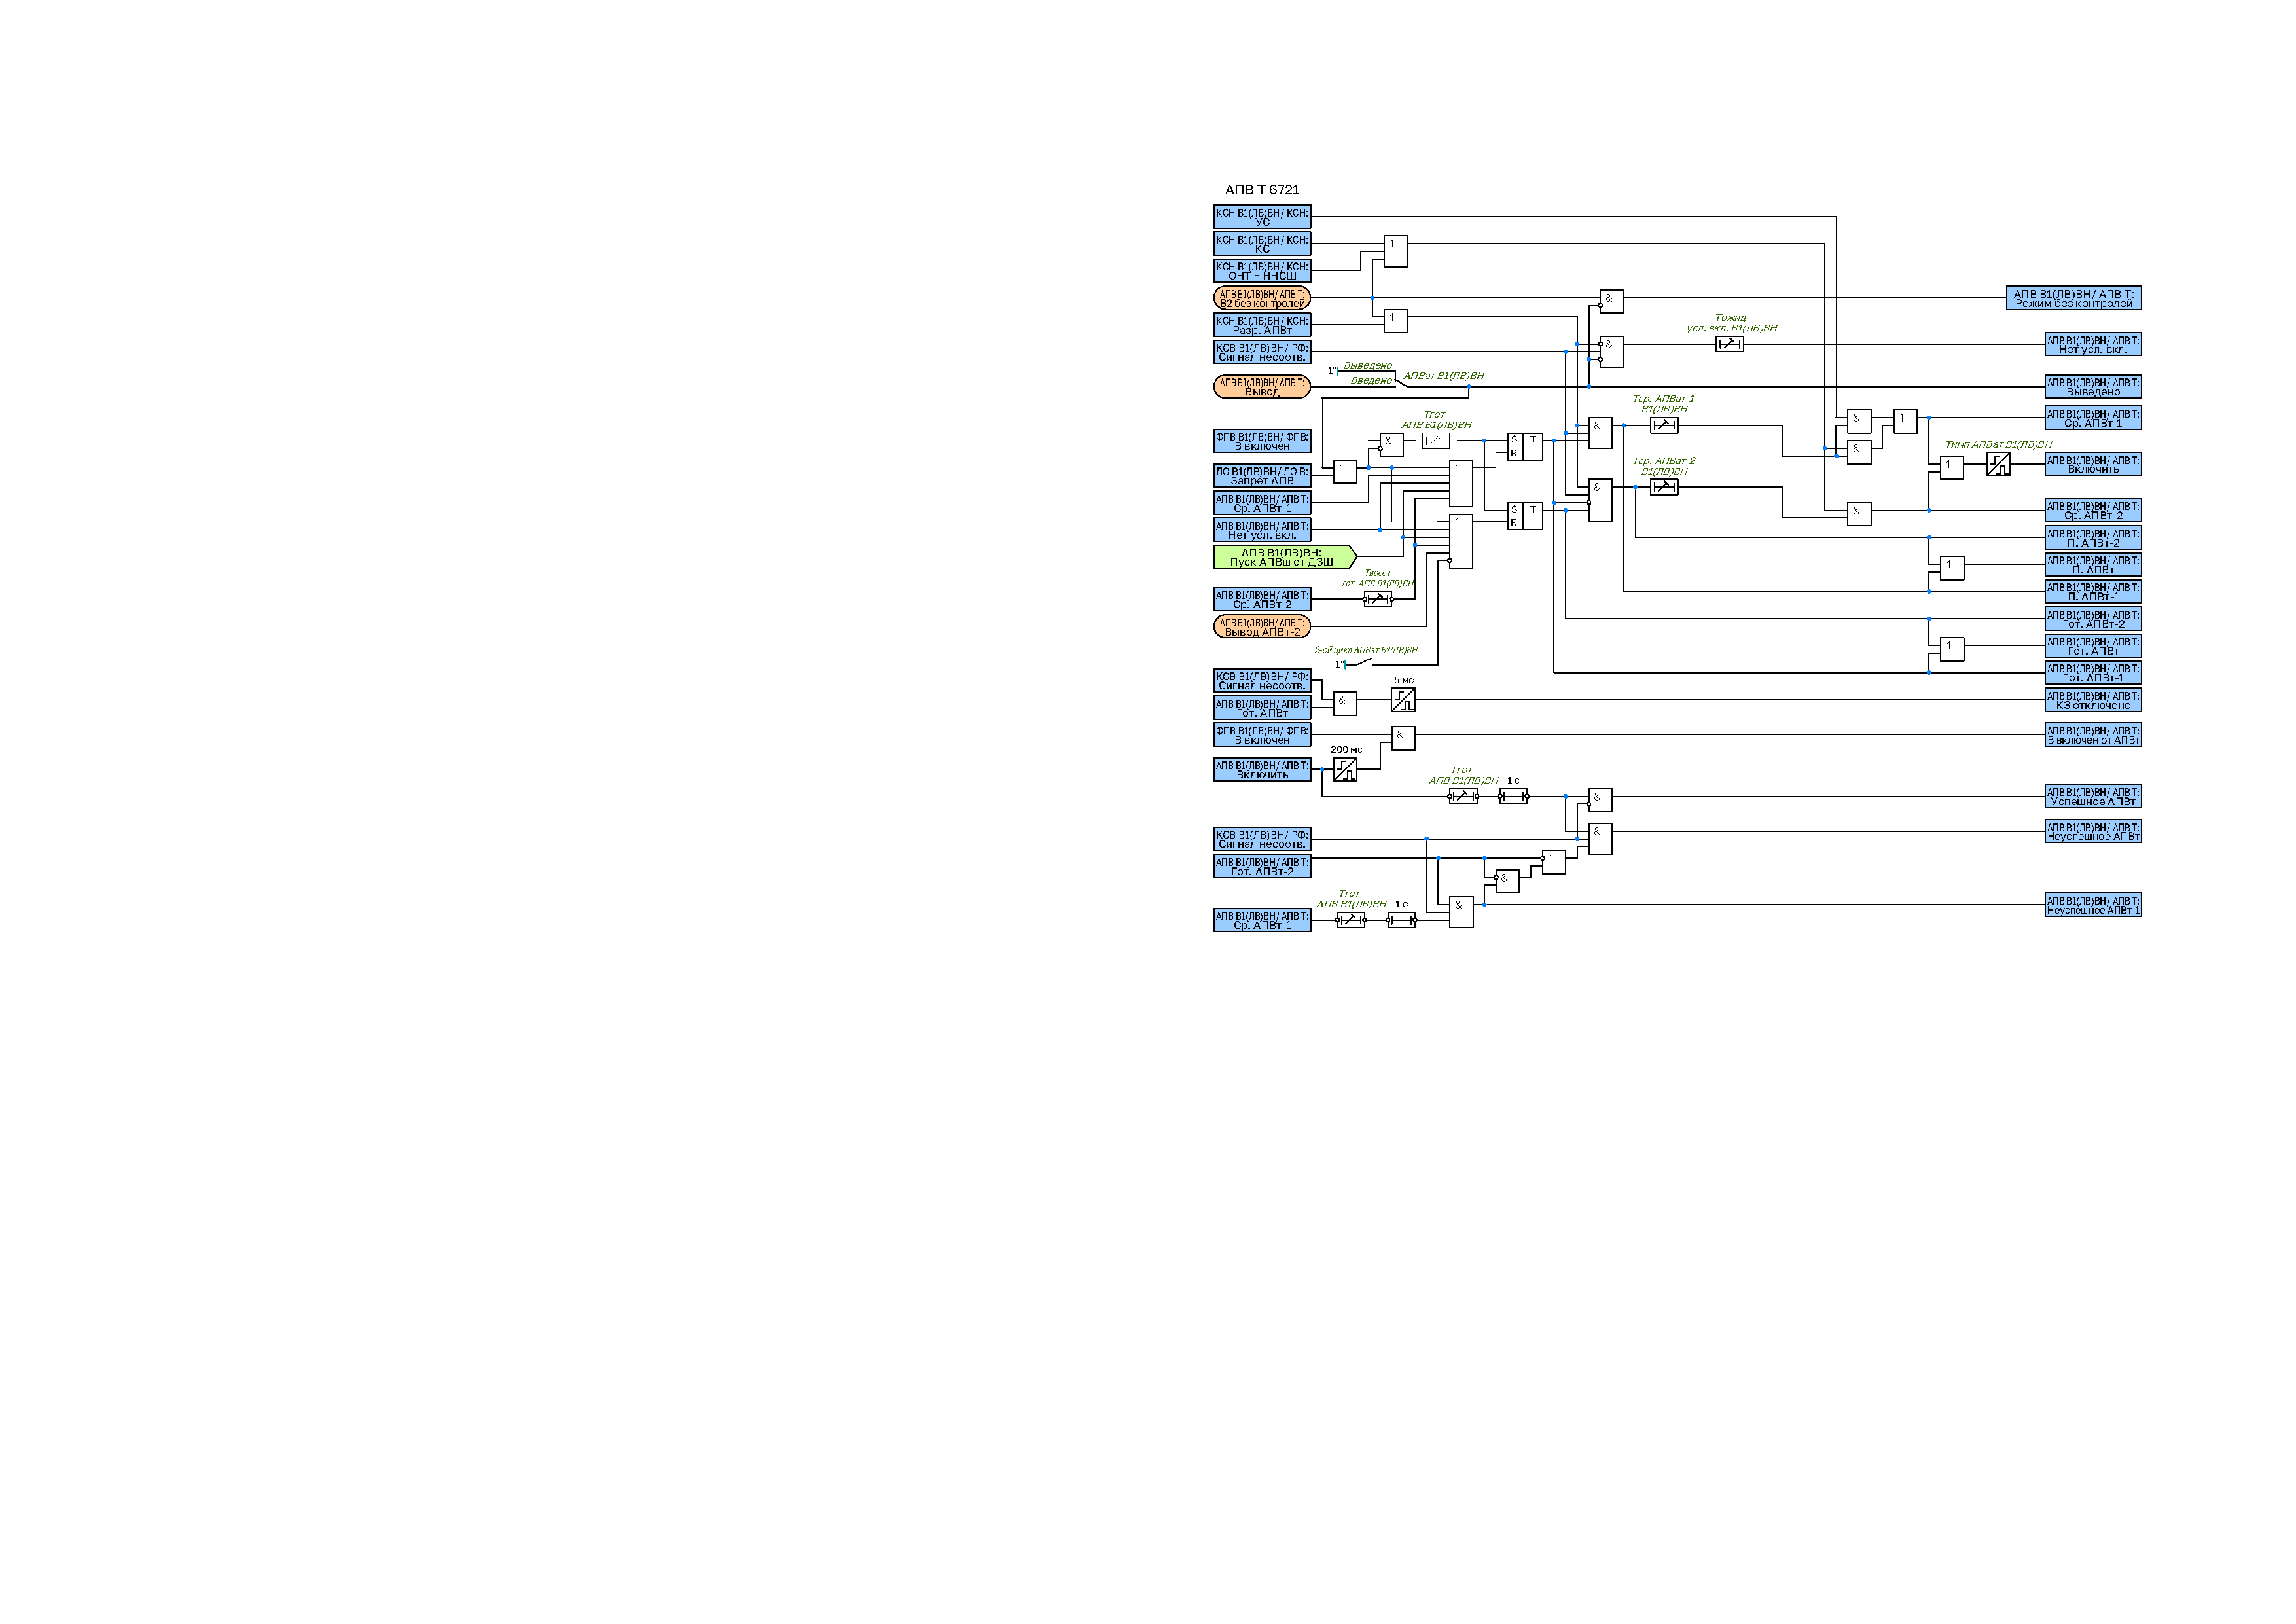
\includegraphics[width=0.9\textwidth,height=0.9\textheight,keepaspectratio]{img31.pdf}
\captionof{figure}{Функциональная схема логики АПВ АТ В1(ЛВ) ВН}\label{pic:APV_AT}
\end{figure}

\item
Пуск АПВ шин осуществляется от внешнего сигнала о срабатывании ДЗШ (входной сигнал ФСУ \textit{«Пуск АПВ В1(ЛВ) ВН от ДЗШ»}). При этом АПВ трансформатор запрещается. АПВ шин выполнено однократным и осуществляется при выполнении условий включения с выдержкой времени \textbf{«Тср АПВш В1(ЛВ) ВН»}. Длительность импульса включения выключателя В1(ЛВ) ВН от АПВ шин задается уставкой \textbf{«Тимп АПВш В1(ЛВ) ВН»}.

\item
Алгоритм работы АПВ СШ ВН приведен на рисунке \ref{pic:APV_SSh}, алгоритм работы АПВ СШ СН выполнен аналогично.

\vspace{2mm}
\begin{figure}[H]
\centering
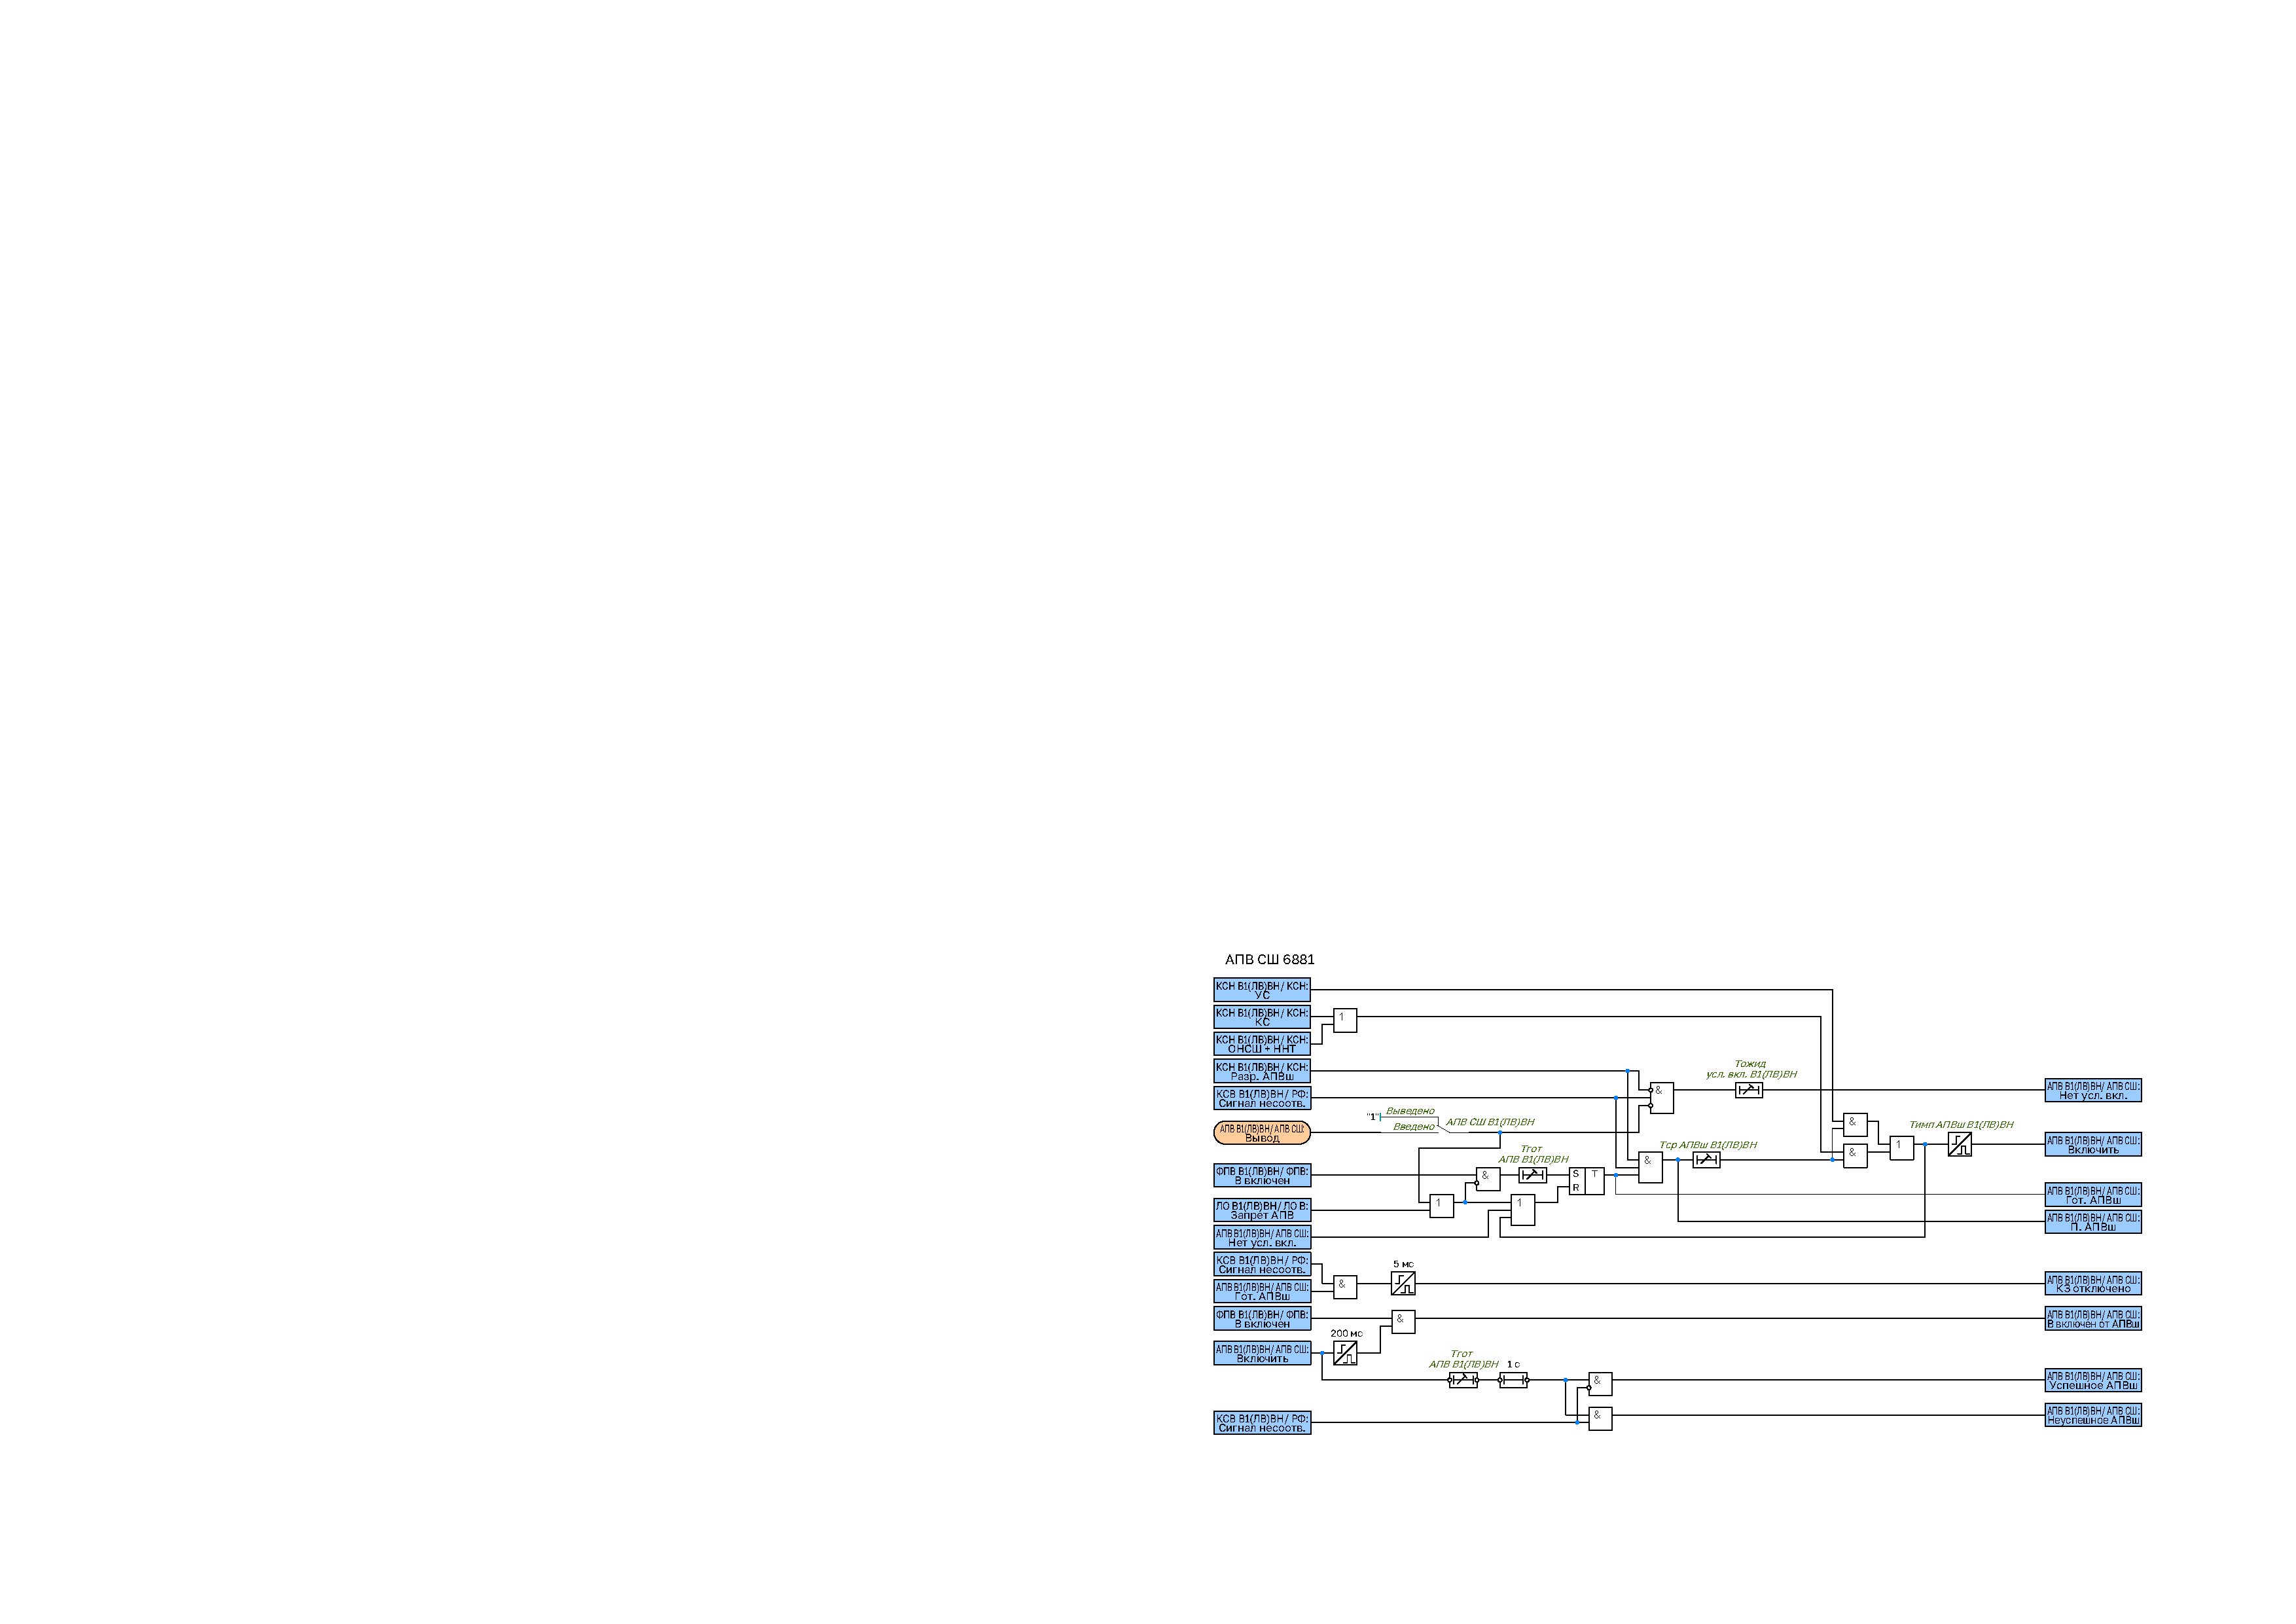
\includegraphics[width=0.9\textwidth,height=0.9\textheight,keepaspectratio]{img32.pdf}
\captionof{figure}{Функциональная схема логики АПВ СШ В1(ЛВ) ВН}\label{pic:APV_SSh}
\end{figure}

\item
В устройстве предусмотрено ограничение ожидания условий включения, которое вводится программным ключом \textbf{«Огр. ожид. усл. вкл. В1(ЛВ) ВН»}. Если в течение выдержки времени \textbf{«Тожид усл. вкл. В1(ЛВ) ВН»} после аварийного отключения не возникают условия включения, то действие АПВ запрещается.

\item
Предусмотрена возможность запрета АПВ при длительно отключенном выключателе, который вводится программным ключом \textbf{«Огр. ожид. пуска АПВ В1(ЛВ) ВН»}. Действие на запрет АПВ осуществляется с выдержкой времени \textbf{«Тожид усл. пуска АПВ В1(ЛВ) ВН»}.


\end{enumerate}
\color{unidarkgreen}{\subsection{Контроль силового выключателя}}
\color{black}

\begin{enumerate}[label=\arabic{section}.\arabic{subsection}.\arabic{enumi}, labelsep=4pt, leftmargin=0pt, itemindent=57pt, itemsep=0pt, parsep=0pt] % если что можно крутить itemsep


\item
Функциональный блок контроля силового выключателя (КСВ) предназначен для обработки технологической информации от выключателя и его цепей управления, а также от трансформатора тока, позволяя определять их состояние, информировать о возможных неисправностях и формировать соответствующую сигнализацию.

\def\Qone{Не определено}
\def\Qtwo{Не определено}

\ifbool{isLV}{
\def\Qone{В1} 
\def\Qtwo{В2} 
\item
В случае присоединения линии к системе через два выключателя для каждого из них можно задействовать свою логику КСВ. Далее приведено обобщенное описание КСВ для силового выключателя.
}{}
\ifbool{isDZAT}{
\item
\def\Qone{В1(ЛВ) ВН} 
\def\Qtwo{В1(ЛВ) СН} 
В случае присоединения автортансформатора к РУ через один выключатель ВН и один выключатель СН для каждого из них можно задействовать свою логику КСВ. Далее приведено обобщенное описание КСВ для силового выключателя.
}{}


\item
Уставки КСВ \Qone~ представлены в таблице \ref{app_set:ksv1}. Уставки КСВ \Qtwo~ представлены в таблице \ref{app_set:ksv2}.

\item
Обобщенная функциональная схема логики контроля выключателя приведена на рисунке \ref{pict_ksv:KSV_control}.

\vspace{2mm}
\begin{figure}[H]
\centering
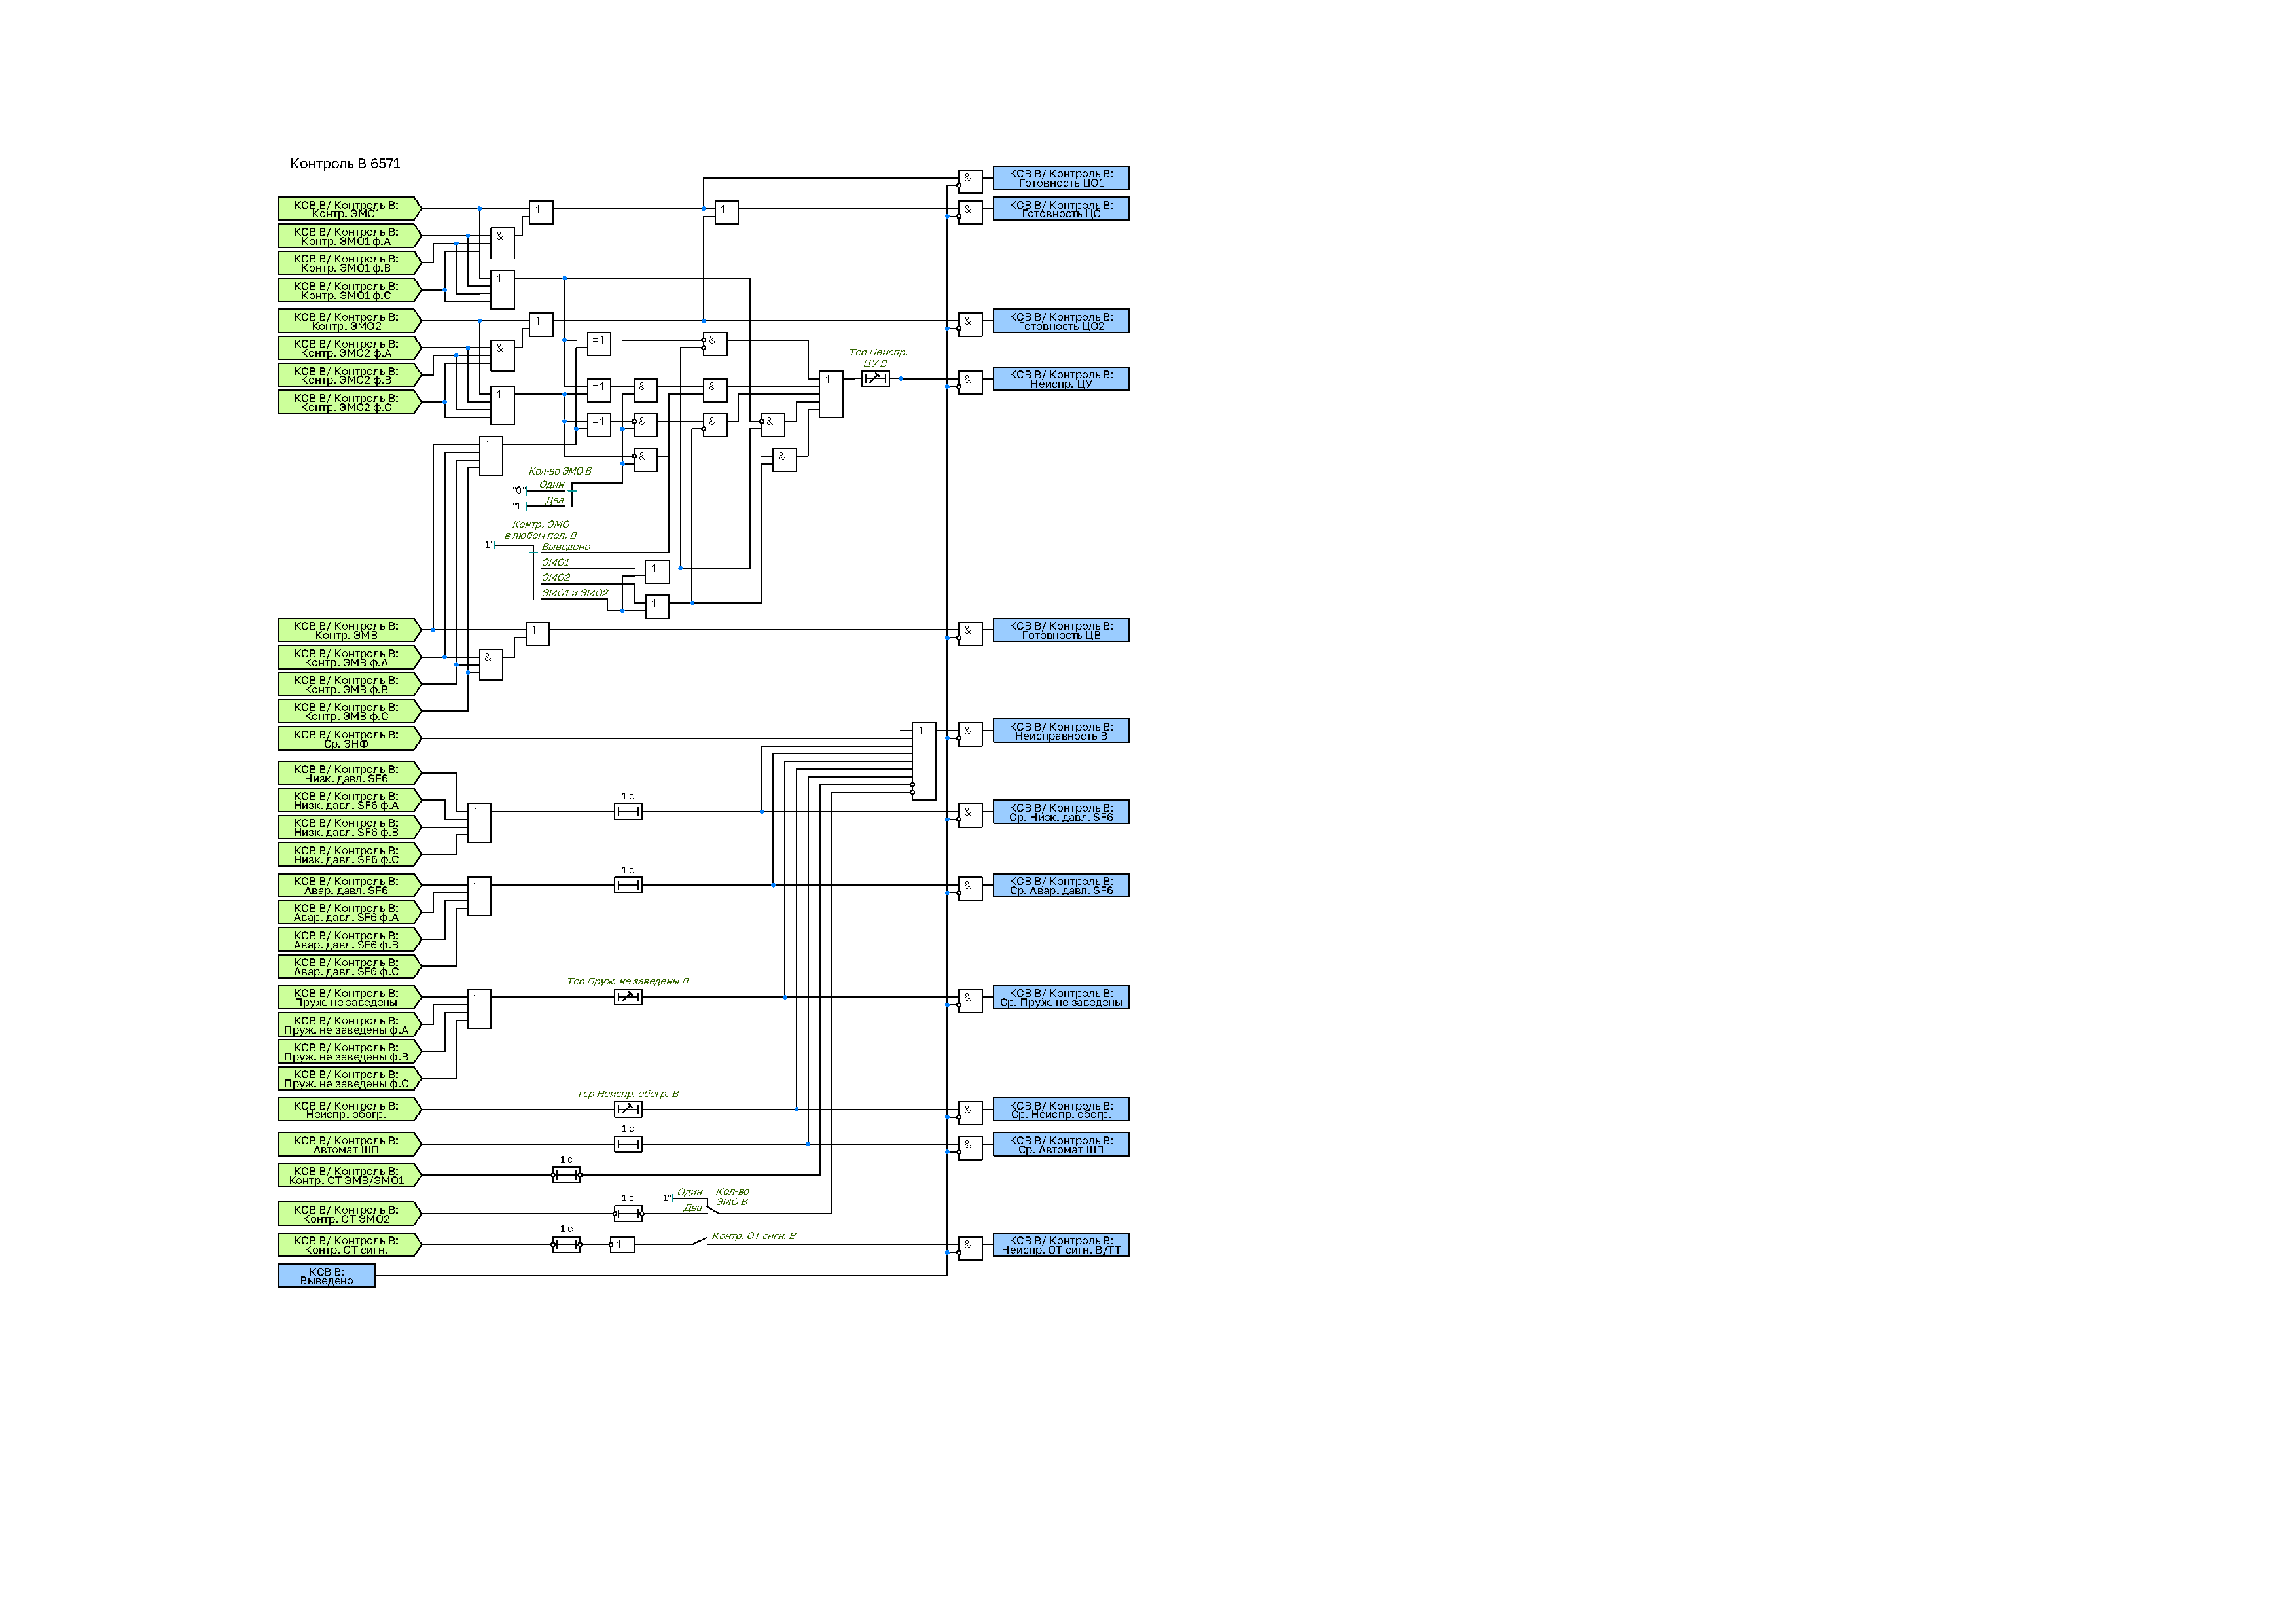
\includegraphics[width=1\textwidth,height=1\textheight,keepaspectratio]{img33.pdf}
\captionof{figure}{Функциональная схема логики контроля выключателя}\label{pict_ksv:KSV_control}
\end{figure}

\item
Контроль готовности привода выключателя осуществляется по внешнему сигналу \textit{«Пруж. не заведены В»}. Сигнал о незаведенном состоянии пружины \textit{«Ср. Пруж. не заведены В»} формируется с выдержкой времени \textbf{«Тср Пруж. не заведены В»}. 

\item
Контроль целостности цепей управления осуществляется по сигналам состояния цепей первой и второй группы электромагнитов отключения (ЭМО1 и ЭМО2) и цепи электромагнита включения (ЭМВ). Наличие второй группы электромагнитов отключения определяется положением программного переключателя \textbf{«Кол-во ЭМО В»}. При одновременном наличии или отсутствии сигналов контроля цепей ЭМО и ЭМВ в течение регулируемой выдержки времени \textbf{«Тср Неиспр. ЦУ В»} формируется сигнал \textit{«Неиспр. ЦУ В»}. Выдержка времени должна быть не менее времени взвода пружины привода выключателя.

\item
Предусмотрен контроль давления элегаза в баке выключателя по внешним сигналам \textit{«Низк. давл. SF6 В»} и \textit{«Авар. давл. SF6 В»} от специальных датчиков давления. Соответствующие сигналы о низком и аварийном давлении элегаза \textit{«Ср. Низк. давл. SF6 В»} и \textit{«Ср. Авар. давл. SF6 В»} формируются с выдержками времени, равными 1 с.

\item
Контроль положения автомата шинок питания осуществляется по внешнему сигналу \textit{«Автомат ШП В»}. Сигнал об отключенном положении автомата \textit{«Ср. Автомат ШП В»} формируется с выдержкой времени выдержкой времени, равной 1 с. 

\item
Обогрев выключателя контролируется по внешнему сигналу \textit{«Неиспр. обогр. В»}. Соответствующий сигнал о неисправности обогрева \textit{«Ср. Неиспр. обогр. В»} формируется с регулируемой выдержкой времени \textbf{«Тср Неиспр. обогр. В»}.

\item
Сигнализация о неисправности выключателя (сигнал \textit{«Неиспр. В»}) срабатывает при наличии одного из сигналов: \textit{«Неиспр. ЦУ В»}, \textit{«Ср. Пруж. не заведены В»}, \textit{«Ср. Низк. давл. SF6 В»}, \textit{«Ср. Авар. давл. SF6 В»}, \textit{«Ср. Автомат ШП В»}, \textit{«Ср. Неиспр. обогр. В»}, а также от сигнала \textit{«Ср. ЗНФ В»}.

\item
Контроль наличия питания цепей сигнализации выключателя и ТТ осуществляется по внешним сигналам \textit{«Контр. опертока ЭМВ/ЭМО1 В»}, \textit{«Контр. опертока ЭМО2 В»} и \textit{«Контр. опертока сигн. В»}. При состоянии «0» одного из сигналов срабатывает сигнализация о неисправности цепей сигнализации выключателя и ТТ (сигнал \textit{«Неиспр. сигн. В1/ТТ В»}) с выдержкой времени 1 с. 



\item
В устройстве также предусмотрен контроль состояния ТТ. Контроль давления элегаза в ТТ осуществляется по внешним сигналам \textit{«Низк. давл. SF6 ТТ В»} и \textit{«Авар. давл. SF6 ТТ В»}. Соответствующие сигналы о низком и аварийном давлении элегаза \textit{«Ср. Низк. давл. SF6 В»} и \textit{«Ср. Авар. давл. SF6 В»} формируются с выдержками времени, равными 1 с. Обогрев ТТ контролируется по внешнему сигналу \textit{«Неиспр. обогр. ТТ В»}. Соответствующий сигнал о неисправности обогрева \textit{«Ср. Неиспр. обогр. ТТ В»}
формируется с регулируемой выдержкой времени \textbf{«Тср Неиспр. обогр. ТТ В»}. По наличию одного из указанных сигналов формируется сигнал о неисправности ТТ \textit{«Неиспр. ТТ В»}. При вводе программного ключа \textbf{«Откл. от Авар. давл. SF6 ТТ В»} предусматривается действие на отключение выключателя при аварийном снижении давления элегаза в ТТ.

\item
Обобщенная функциональная схема логики контроля ТТ выключателя приведена на рисунке \ref{pict_ksv:KSV_control_TT_B1}.

\vspace{2mm}
\begin{figure}[H]
\centering
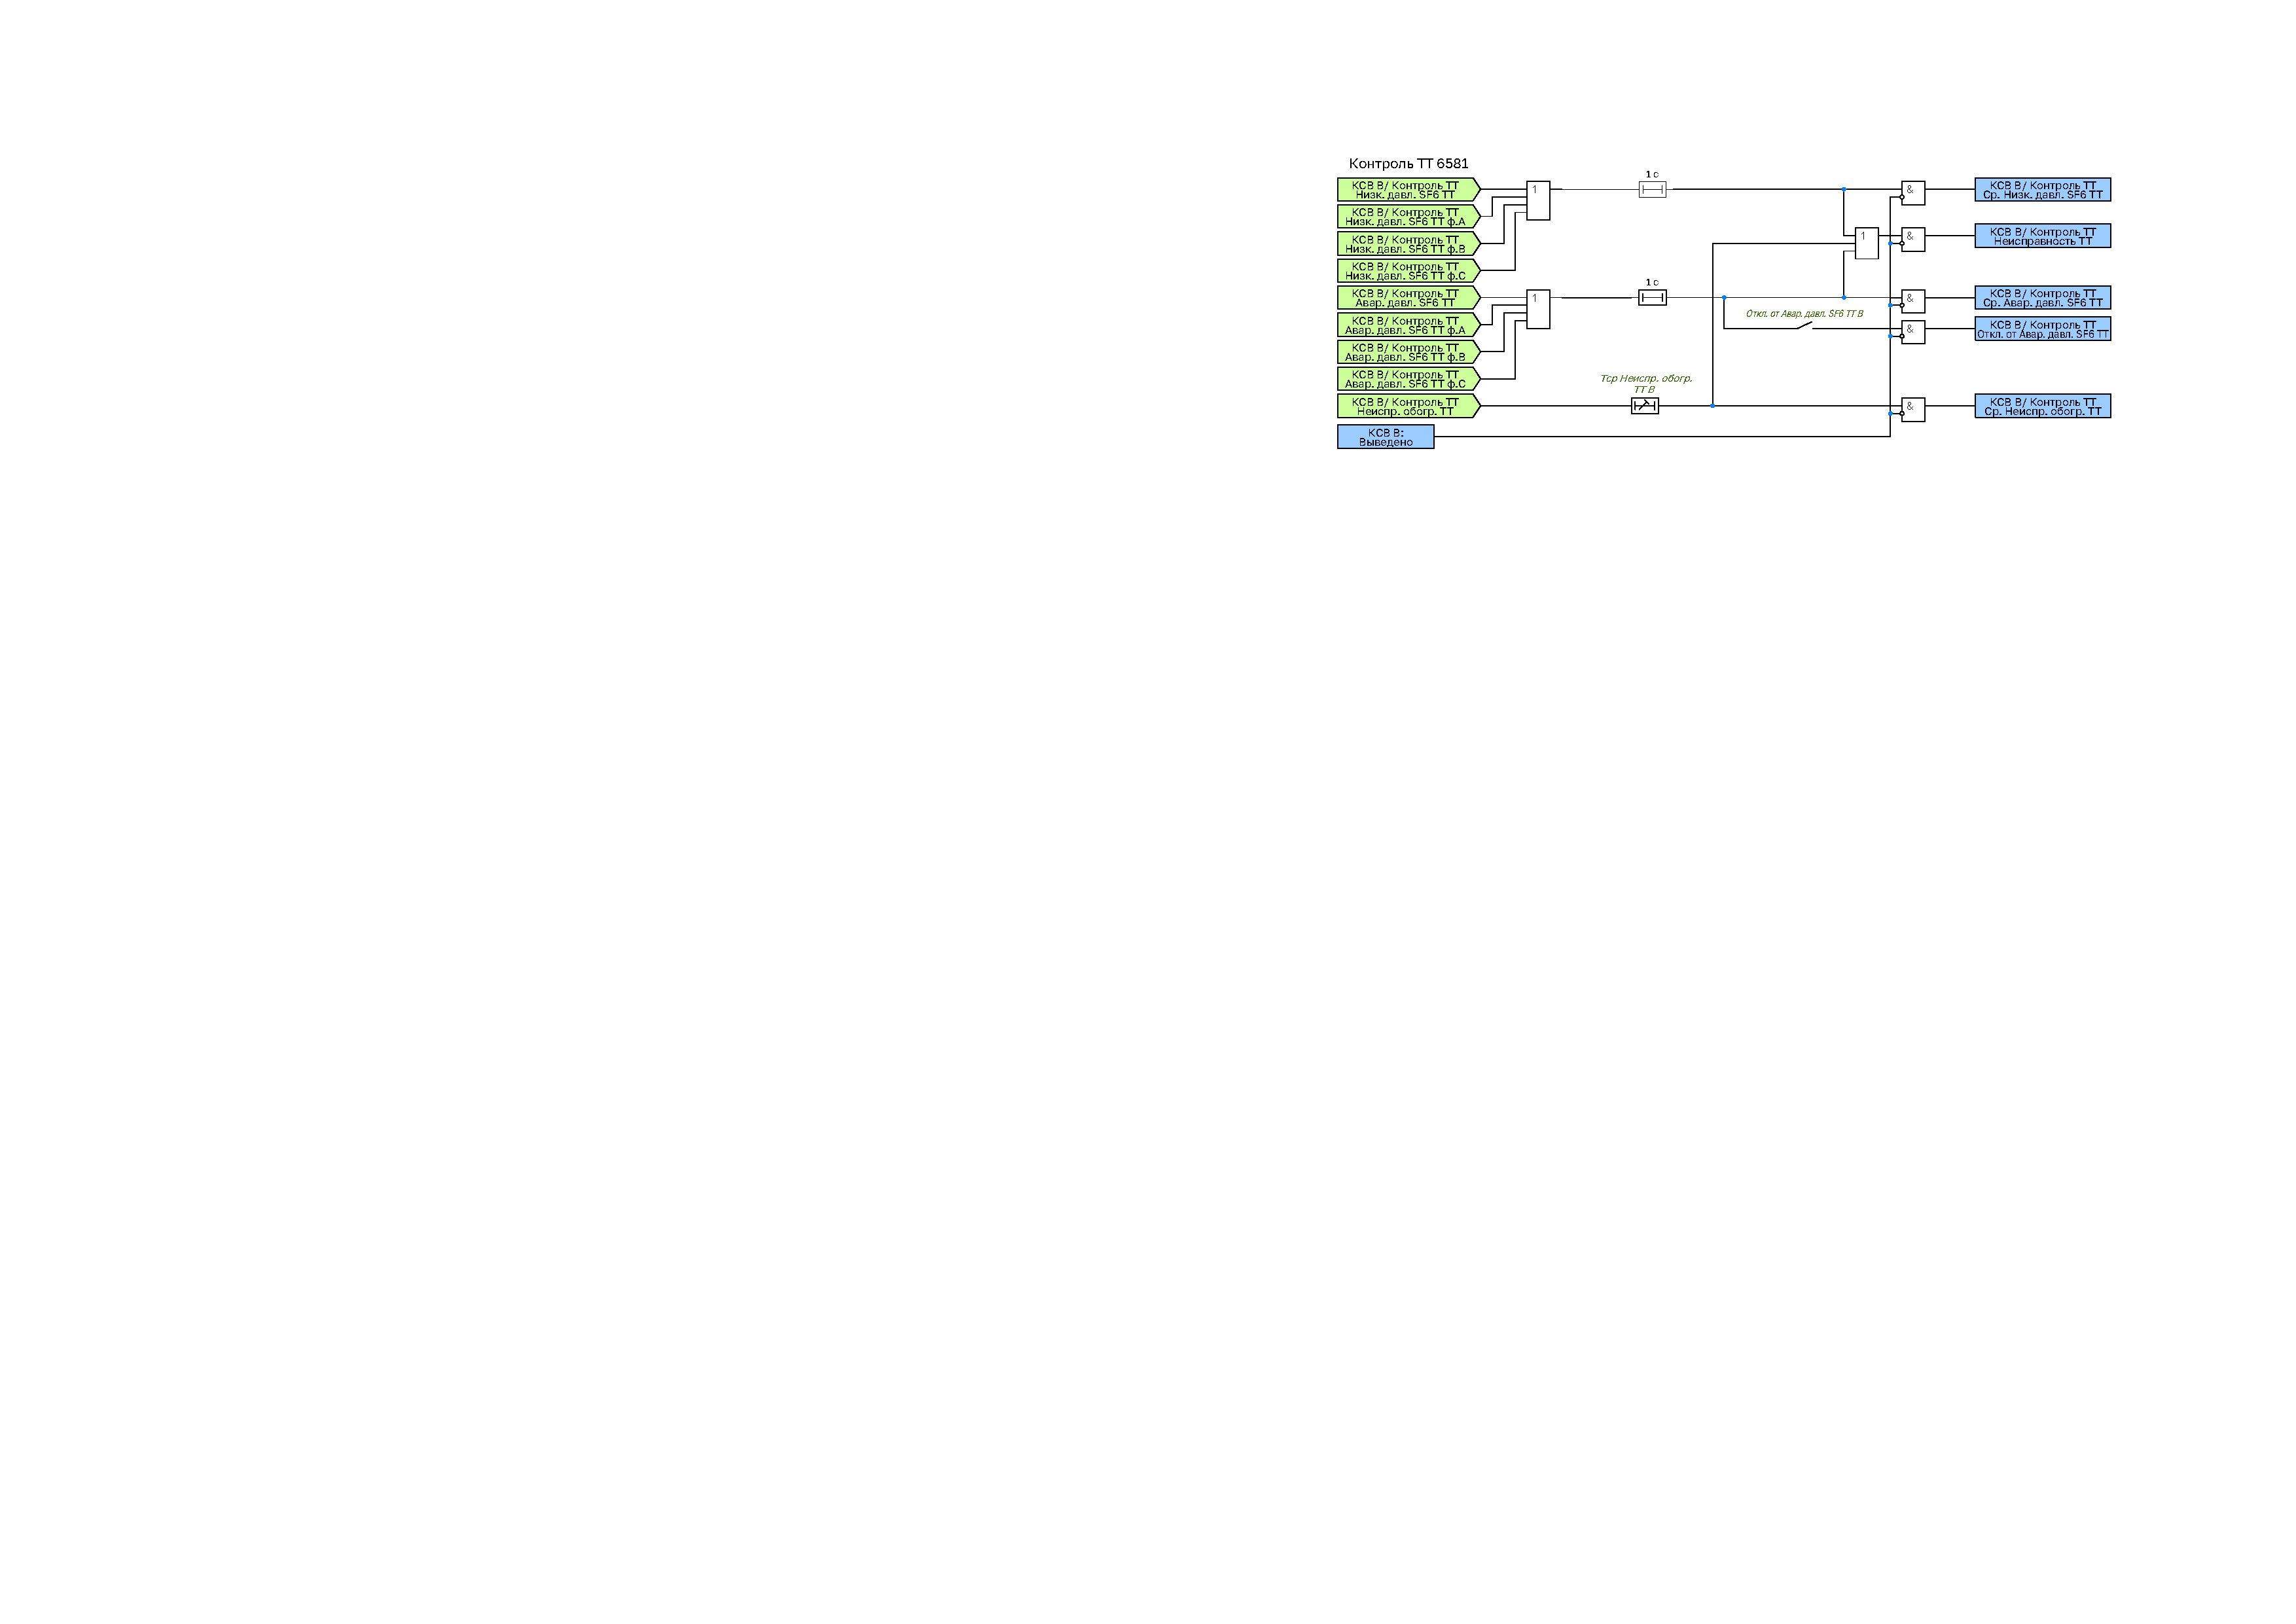
\includegraphics[width=1\textwidth,height=1\textheight,keepaspectratio]{img34.pdf}
\captionof{figure}{Функциональная схема логики контроля ТТ выключателя}\label{pict_ksv:KSV_control_TT_B1}
\end{figure}



\item
Для электромагнитов управления предусмотрена защита от длительного протекания тока. Контроль протекания тока через ЭМВ, ЭМО1 и ЭМО2 осуществляется при помощи токовых реле, положения контактов которых должны быть заведены на соответствующие входные сигналы ФСУ «Работа ЭМВ В», «Работа ЭМО1 В», «Работа ЭМО2 В». При длительном протекании тока по цепям ЭМО1 и ЭМВ формируется сигнал «Обест. ЭМО1 и ЭМВ В», действующий на независимый расцепитель автомата питания цепей ЭМО1 и ЭМВ.

\item
Аналогично при длительном протекании тока по цепи ЭМО2 формируется сигнал \textit{«Обест. ЭМО2 В»} для действия на независимый расцепитель автомата питания цепи ЭМО2. Регулируемые выдержки времени \textbf{«Тср защиты ЭМВ В»}, \textbf{«Тср защиты ЭМО1 В»} и \textbf{«Тср защиты ЭМО2 В»} определяют время срабатывания на обесточивание ЭМВ, ЭМО1 и ЭМО2 соответственно. Кроме того, наличие сигнала \textit{«Ср. Авар. давл. SF6 В»} действует на обесточивание всех электромагнитов.

\item
Обобщенная функциональная схема логики защиты ЭМУ выключателя приведена на рисунке \ref{pict_ksv:KSV_EMU_protection}.

\vspace{2mm}
\begin{figure}[H]
\centering
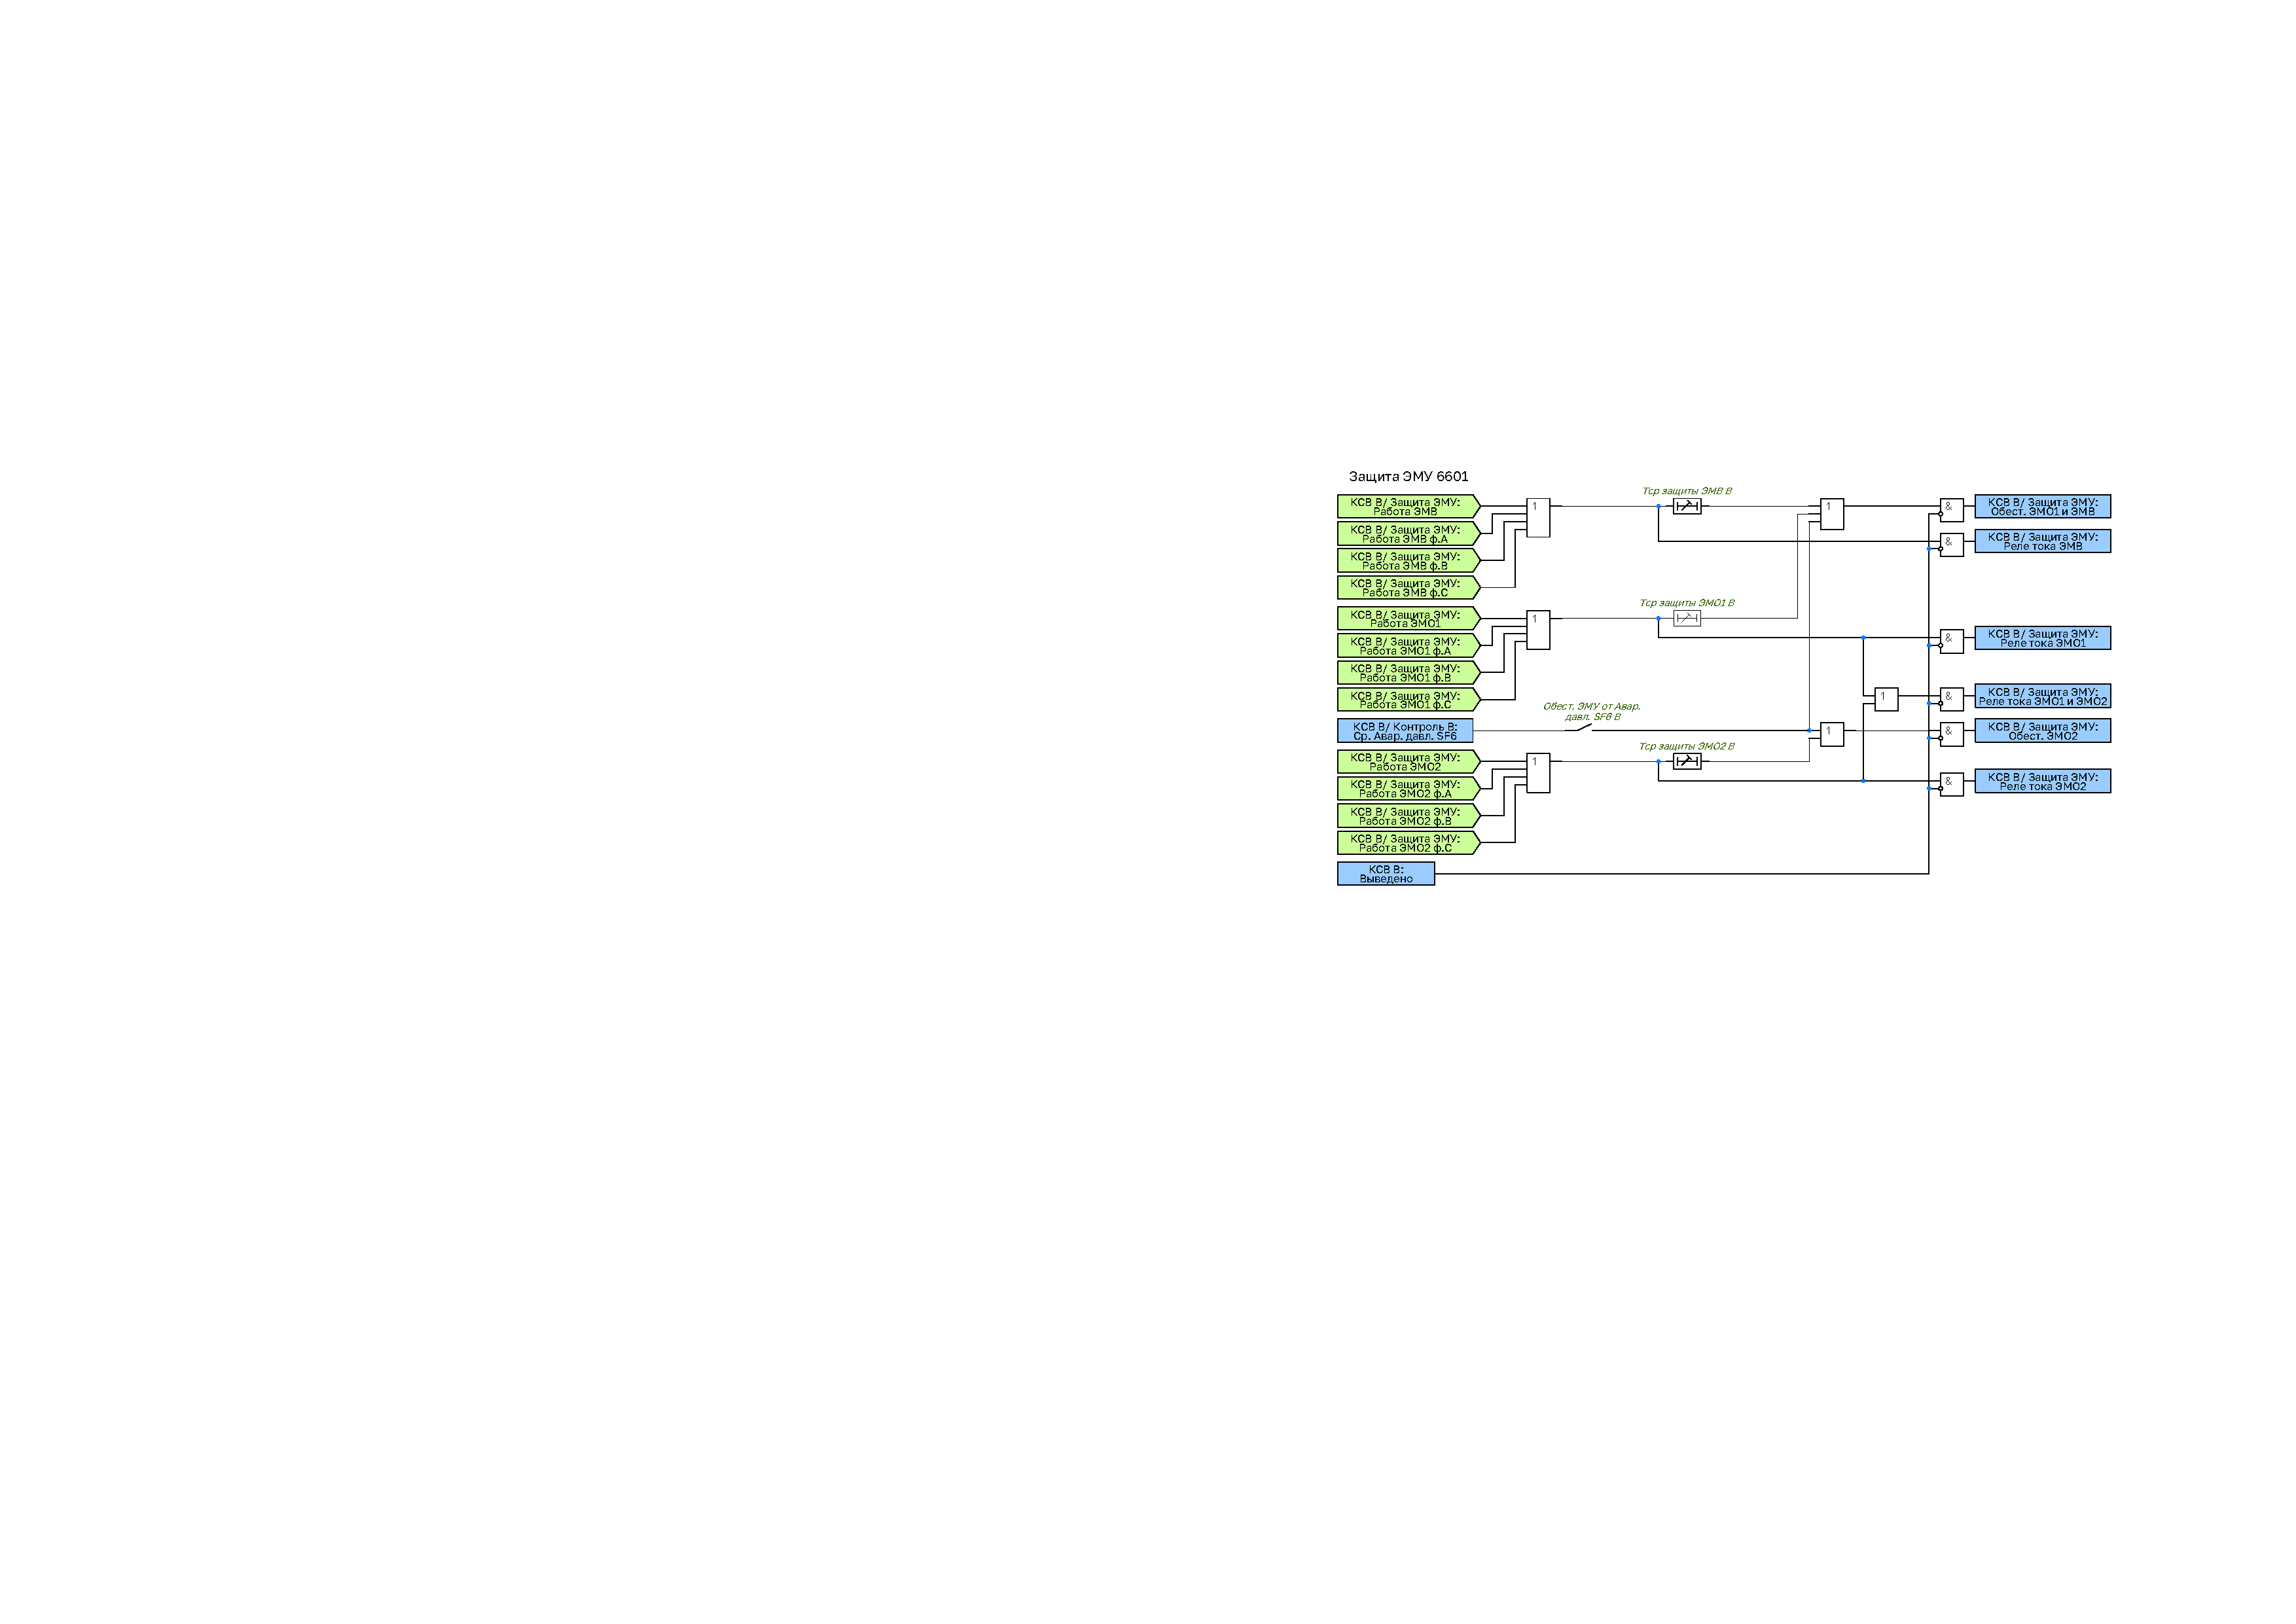
\includegraphics[width=1\textwidth,height=1\textheight,keepaspectratio]{img35.pdf}
\captionof{figure}{Функциональная схема логики защиты ЭМУ выключателя}\label{pict_ksv:KSV_EMU_protection}
\end{figure}



\item 
В устройстве предусмотрена логика формирования блокировки команд на включение и отключение выключателя.

\item
На блокировку отключения выключателя действует сигнал \textit{«Ср. Авар. давл. SF6 В»}. На блокировку включения действуют сигналы \textit{«Ср. Авар. давл. SF6 В»}, \textit{«Неиспр. ЦУ В»}, \textit{«Ср. Пруж. не заведены В»}, \textit{«Ср. Автомат ШП В»}.

\item
Также предусмотрена блокировка отключения от внешнего сигнала \textit{«Внеш. блок. откл. В»}, блокировка включения от внешнего сигнала \textit{«Внеш. блок. вкл. В»} и блокировка управления (как включения, так и отключения) от внешнего сигнала \textit{«Внеш. блок. упр. В»}.

\item
Обобщенная функциональная схема логики блокировки управления выключателя приведена на рисунке \ref{pict_ksv:KSV_control_block}.

\vspace{2mm}
\begin{figure}[H]
\centering
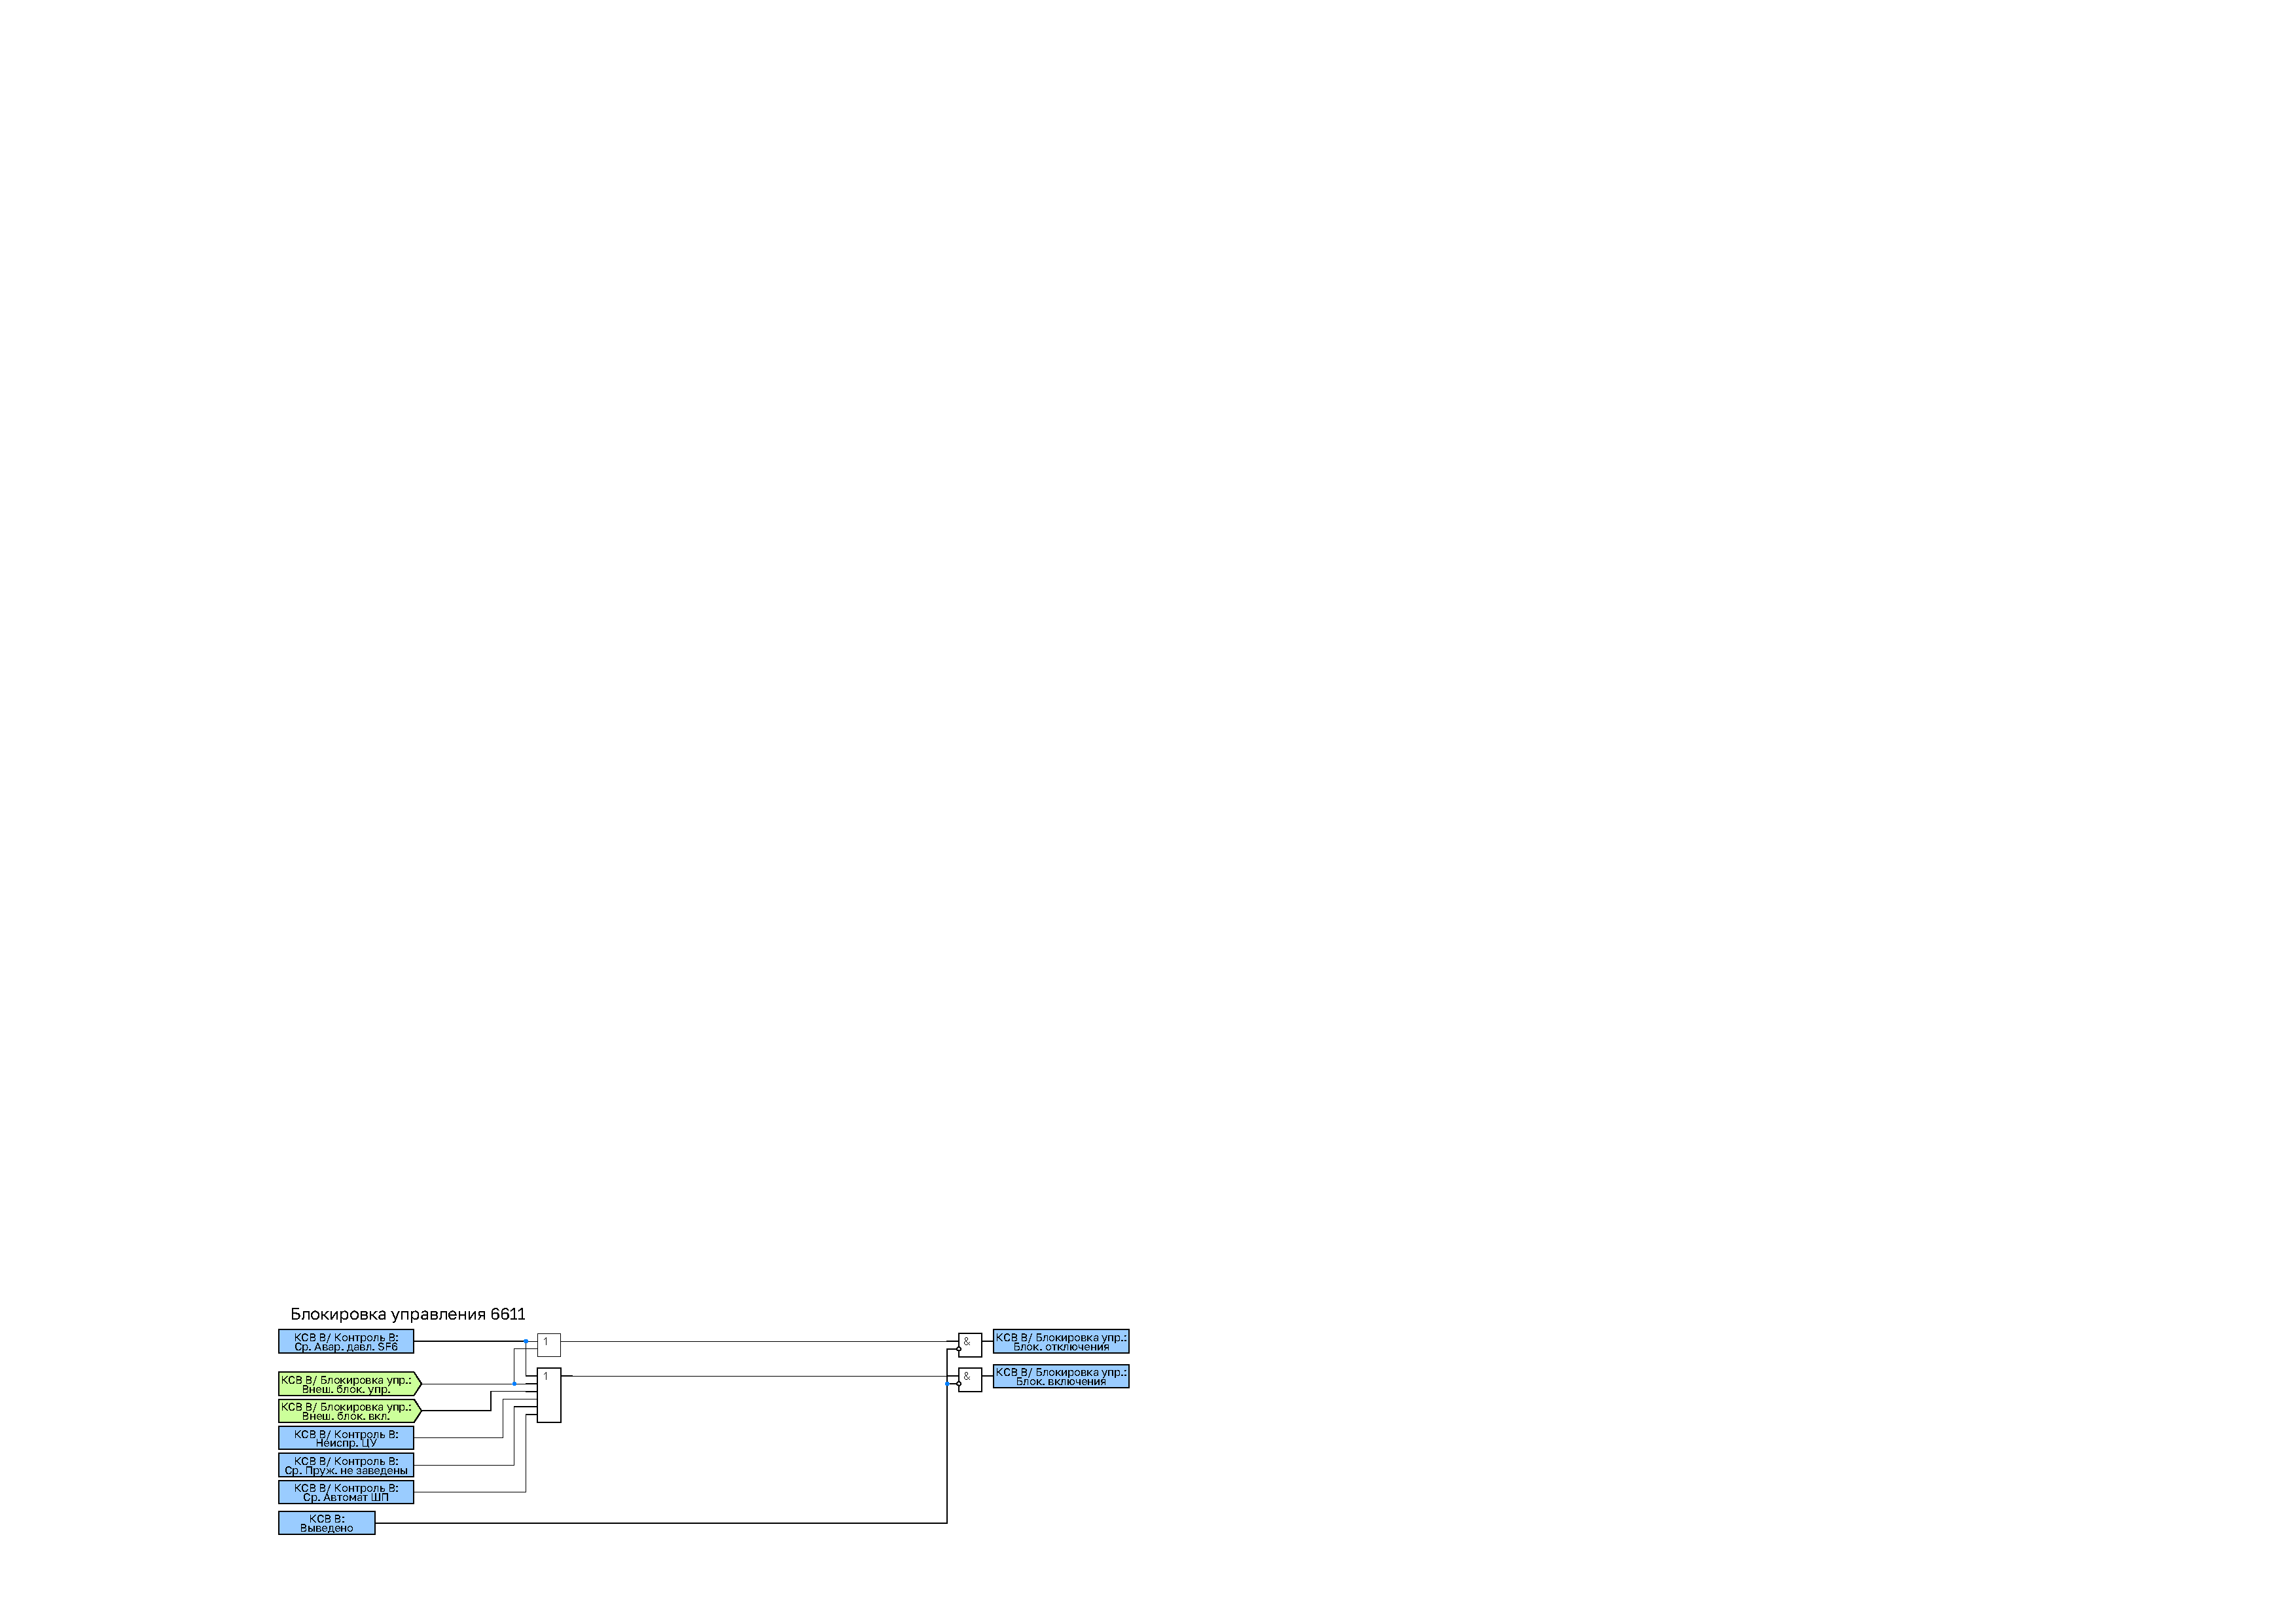
\includegraphics[width=1\textwidth,height=1\textheight,keepaspectratio]{img36.pdf}
\captionof{figure}{Функциональная схема логики блокировки управления выключателя}\label{pict_ksv:KSV_control_block}
\end{figure}


\item
В устройстве предусмотрена программная фиксация команд или включенного положения выключателя в зависимости от положения программного переключателя \textbf{«Реле фиксации В1»}. В положении \textit{«РФК»} фиксируется команда включения, в положении \textit{«РФП»} – включенное положение. Квитирование сигнала фиксации \textit{«РФ В1»} может осуществляться от сброса сигнализации или подачей оперативной команды на отключение. При отключении выключателя от защит и наличии сигнала \textit{«РФ В1»} формируется сигнал о факте аварийного отключения выключателя \textit{«Сигнал несоотв. В1»}, необходимый для работы АПВ.

\item
Обобщенная функциональная схема логики реле фиксации выключателя приведена на рисунке \ref{pict_ksv:KSV_relay_fix_B1}.

\vspace{2mm}
\begin{figure}[H]
\centering
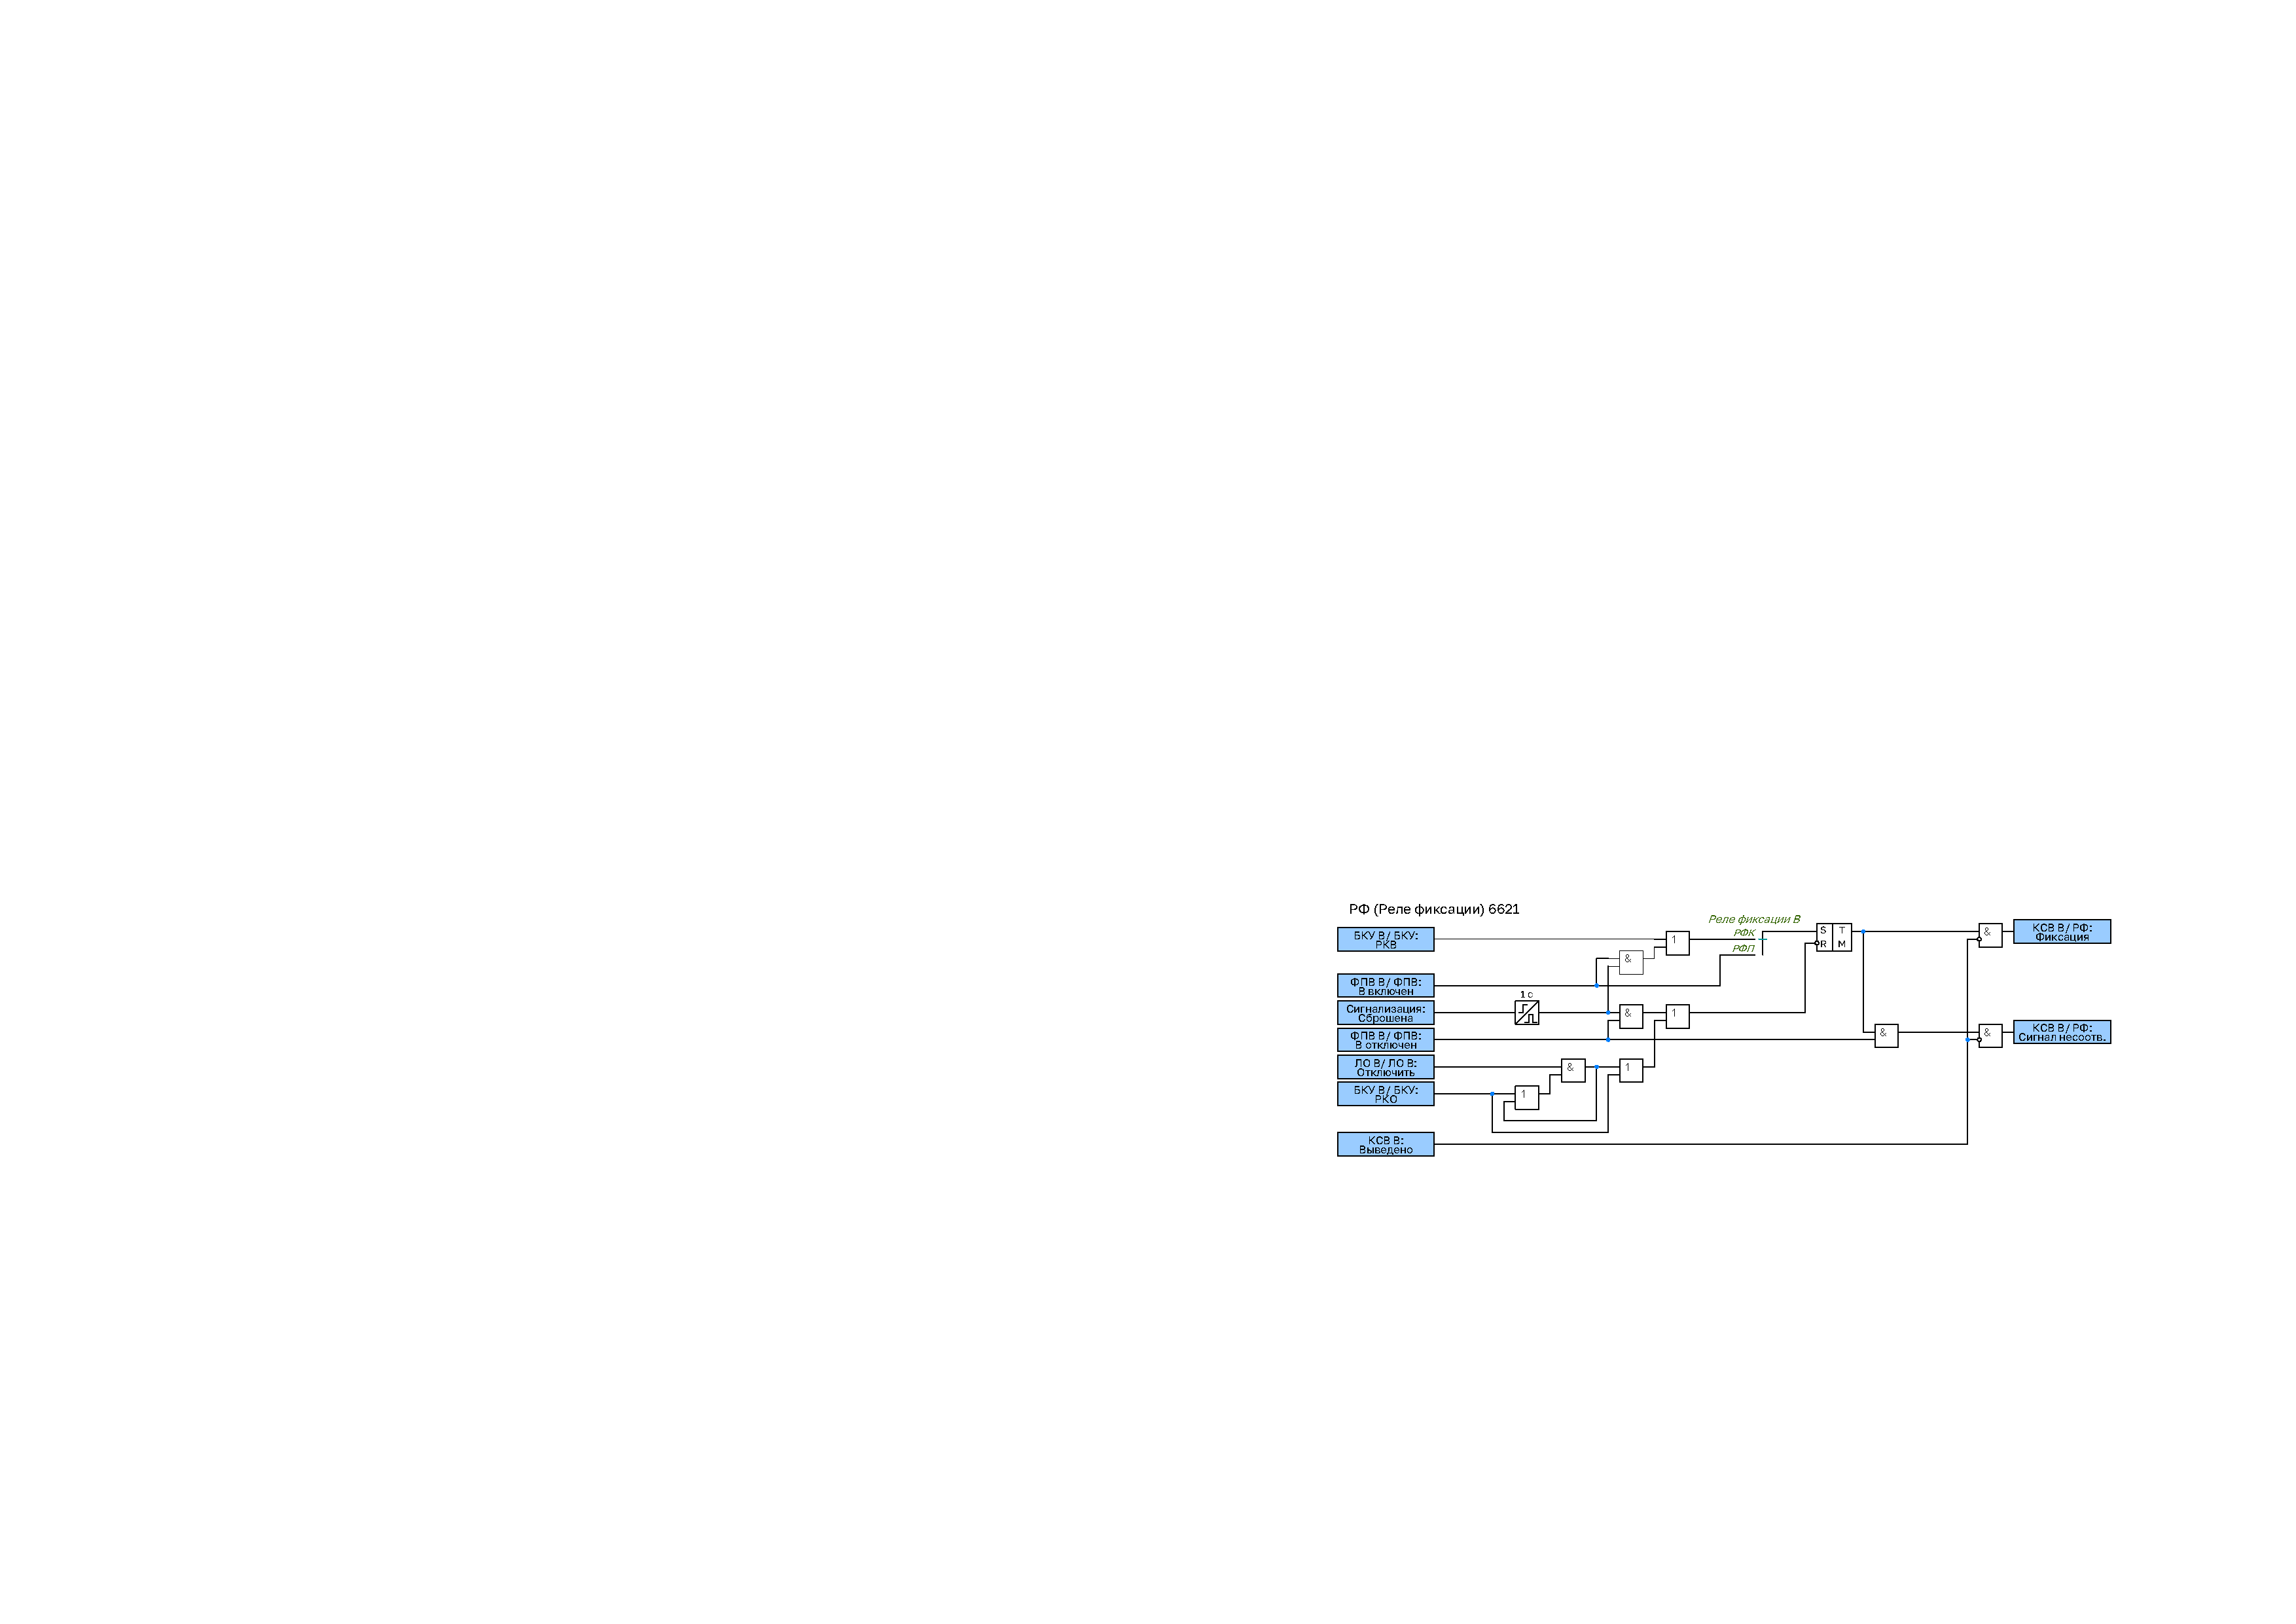
\includegraphics[width=1\textwidth,height=1\textheight,keepaspectratio]{img37.pdf}
\captionof{figure}{Функциональная схема логики реле фиксации выключателя}\label{pict_ksv:KSV_relay_fix_B1}
\end{figure}

\end{enumerate}
\color{unidarkgreen}{\subsection{Логика внешних отключений}}
\color{black}

\begin{enumerate}[label=\arabic{section}.\arabic{subsection}.\arabic*,  align=left, labelsep=4pt, leftmargin=0pt, itemindent=57pt]

\item
Логика внешний отключений РЗ ВН выводится накладками \textbf{«ЛО внеш РЗ ВН»}.

\item
Команда на срабатывание \textit{«СР. ЛО внеш РЗ ВН»} формируются при возникновении одного из следующих событий:
\begin{itemize}
\item от сигнала \textit{«Откл. от УРОВ ВН»} при отключенном положении \textit{«ОР ОВ ВН»} или при включённом положении \textit{«ОР ОВ ВН»} от \textit{«Откл. от УРОВ ОВ ВН»};
\item Откл. ДЗШ ВН;
\item Откл. от УРОВ РЗ ЛЭП ВН;
\item Откл. от УРОВ РЗ ЛЭП ВН ОВ;
\item Откл от ЗНР смеж СКРМ ВН.
\end{itemize}

\item
Запрет АПВ ВН внешними РЗ \textit{«З. АПВ ВН внеш РЗ»} формируются при возникновении одного из следующих событий:
\begin{itemize}
\item от \textit{«Откл. от УРОВ ВН»} при отключенном положении \textit{«ОР ОВ ВН»} или при включённом положении \textit{«ОР ОВ ВН»} от \textit{«Откл. от УРОВ ОВ ВН»};
\item от \textit{«Откл. от УРОВ РЗ ЛЭП ВН»}, при включенной накладке \textbf{«ЗАПВ УРОВ ЛЭП ВН»};
\item Откл. от УРОВ РЗ ЛЭП ВН ОВ;
\item Откл от ЗНР смеж СКРМ ВН;
\item Запрет АПВ от ДЗШ ВН.
\end{itemize}

\vspace{2mm}
\begin{figure}[H]
\centering
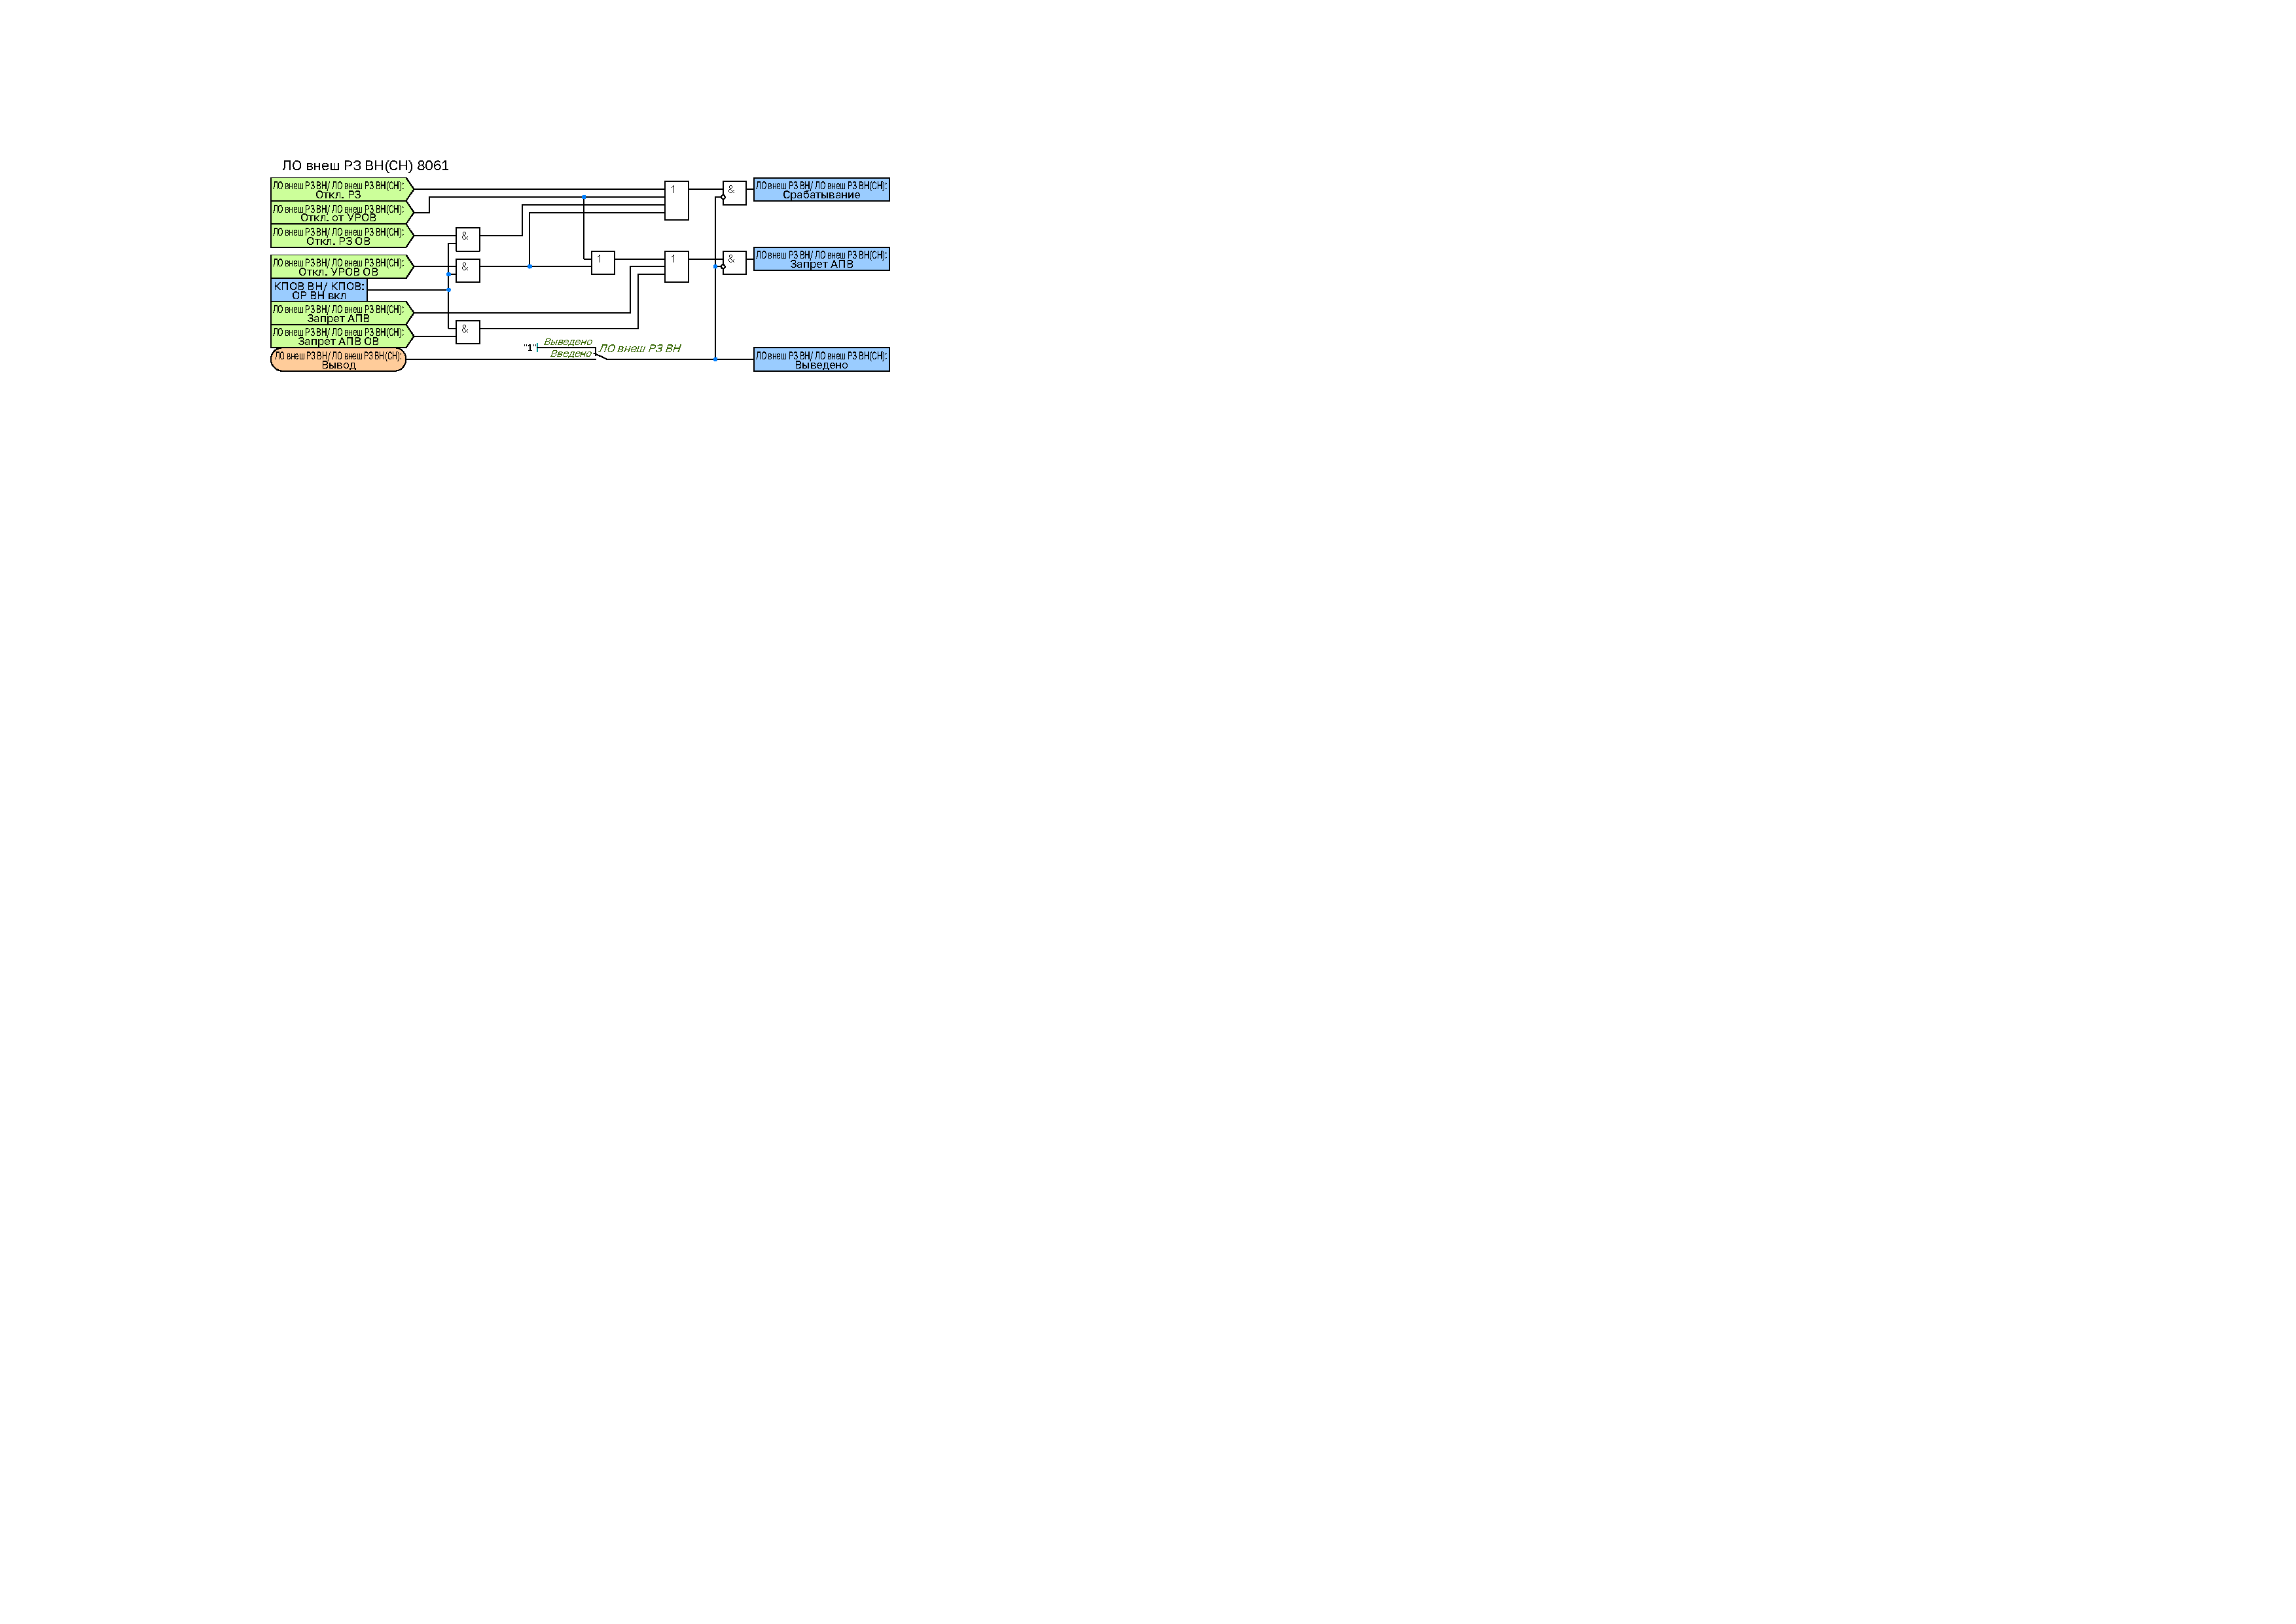
\includegraphics[width=1\textwidth,height=1\textheight,keepaspectratio]{img38.pdf}
\captionof{figure}{Функциональная схема логики внешних отключений ВН}\label{pic:LO_VN}
\end{figure}

Уставки ЛО внеш ВН приведены в таблице \ref{app_set:lovneshvn}.

\item
Логика внешний отключений РЗ СН выводится накладками \textbf{«ЛО внеш РЗ СН}.

\item
Команда на срабатывание \textit{«СР. ЛО внеш РЗ CН»} формируются при возникновении одного из следующих событий:
\begin{itemize}
\item от сигнала \textit{«Откл. от УРОВ СН»} при отключенном положении \textit{«ОР ОВ СН»} или при включённом положении \textit{«ОР ОВ СН»} от \textit{«Откл. от УРОВ ОВ СН»};
\item Откл. ДЗШ СН;
\item Откл. от УРОВ РЗ ЛЭП СН;
\item Откл. от УРОВ РЗ ЛЭП СН ОВ;
\item Откл от ЗНР смеж СКРМ СН.
\end{itemize}

\item
Запрет АПВ ВН внешними РЗ \textit{«З. АПВ СН внеш РЗ»} формируются при возникновении одного из следующих событий:
\begin{itemize}
\item от \textit{«Откл. от УРОВ СН»} при отключенном положении \textit{«ОР ОВ СН»} или при включённом положении \textit{«ОР ОВ СН»} от \textit{«Откл. от УРОВ ОВ СН»};
\item от \textit{«Откл. от УРОВ РЗ ЛЭП СН»}, при включенной накладке \textbf{«ЗАПВ УРОВ ЛЭП СН»};
\item Откл. от УРОВ РЗ ЛЭП СН ОВ;
\item Откл от ЗНР смеж СКРМ СН;
\item Запрет АПВ от ДЗШ СН.
\end{itemize}

\vspace{2mm}
\begin{figure}[H]
\centering
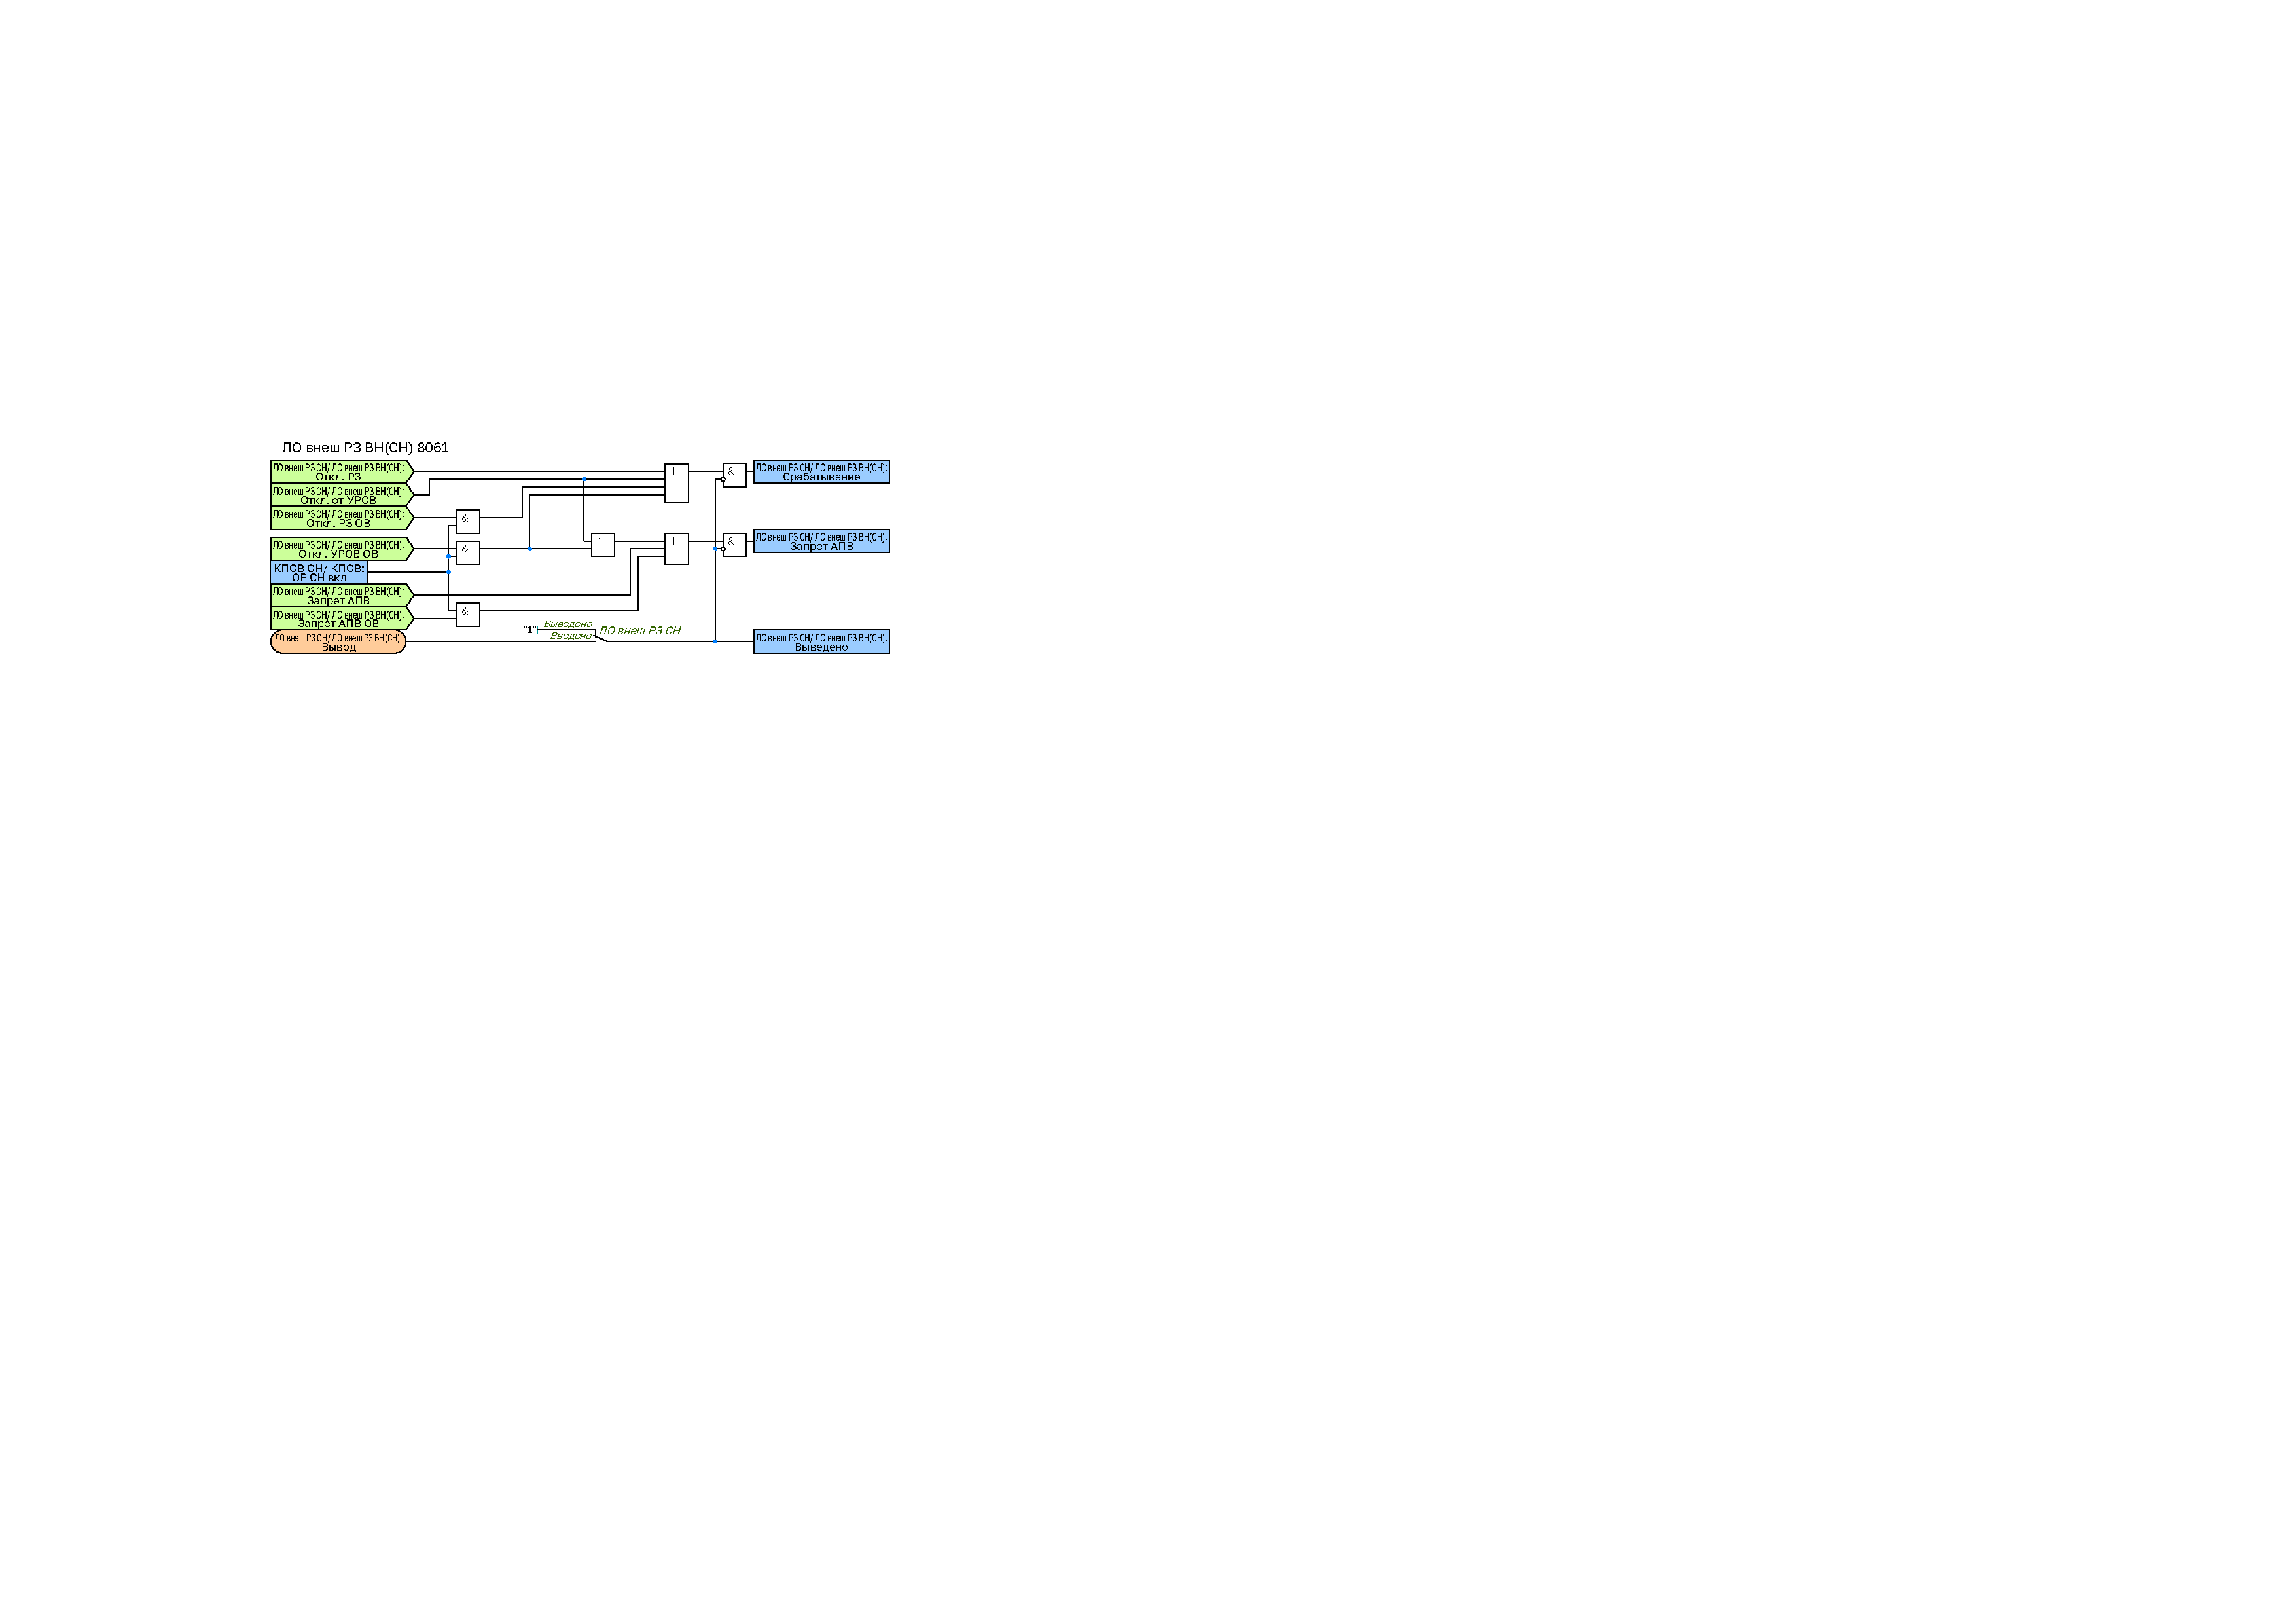
\includegraphics[width=1\textwidth,height=1\textheight,keepaspectratio]{img39.pdf}
\captionof{figure}{Функциональная схема логики внешних отключений СН}\label{pic:LO_SN}
\end{figure}

\item
Уставки ЛО внеш СН приведены в таблице \ref{app_set:lovneshsn}.

\item
Логика внешний отключений РЗ НН выводится накладками \textbf{«ЛО внеш РЗ НН}.

\item
Команда на срабатывание \textit{«СР. ЛО внеш РЗ НН»} формируются при возникновении одного из следующих событий:
\begin{itemize}
\item Откл. ДЗО;
\item Откл от УРОВ НН1;
\item Откл от УРОВ НН2;
\item Откл от ЗДЗ НН1;
\item Откл от ЗДЗ НН2.
\end{itemize}

\vspace{2mm}
\begin{figure}[H]
\centering
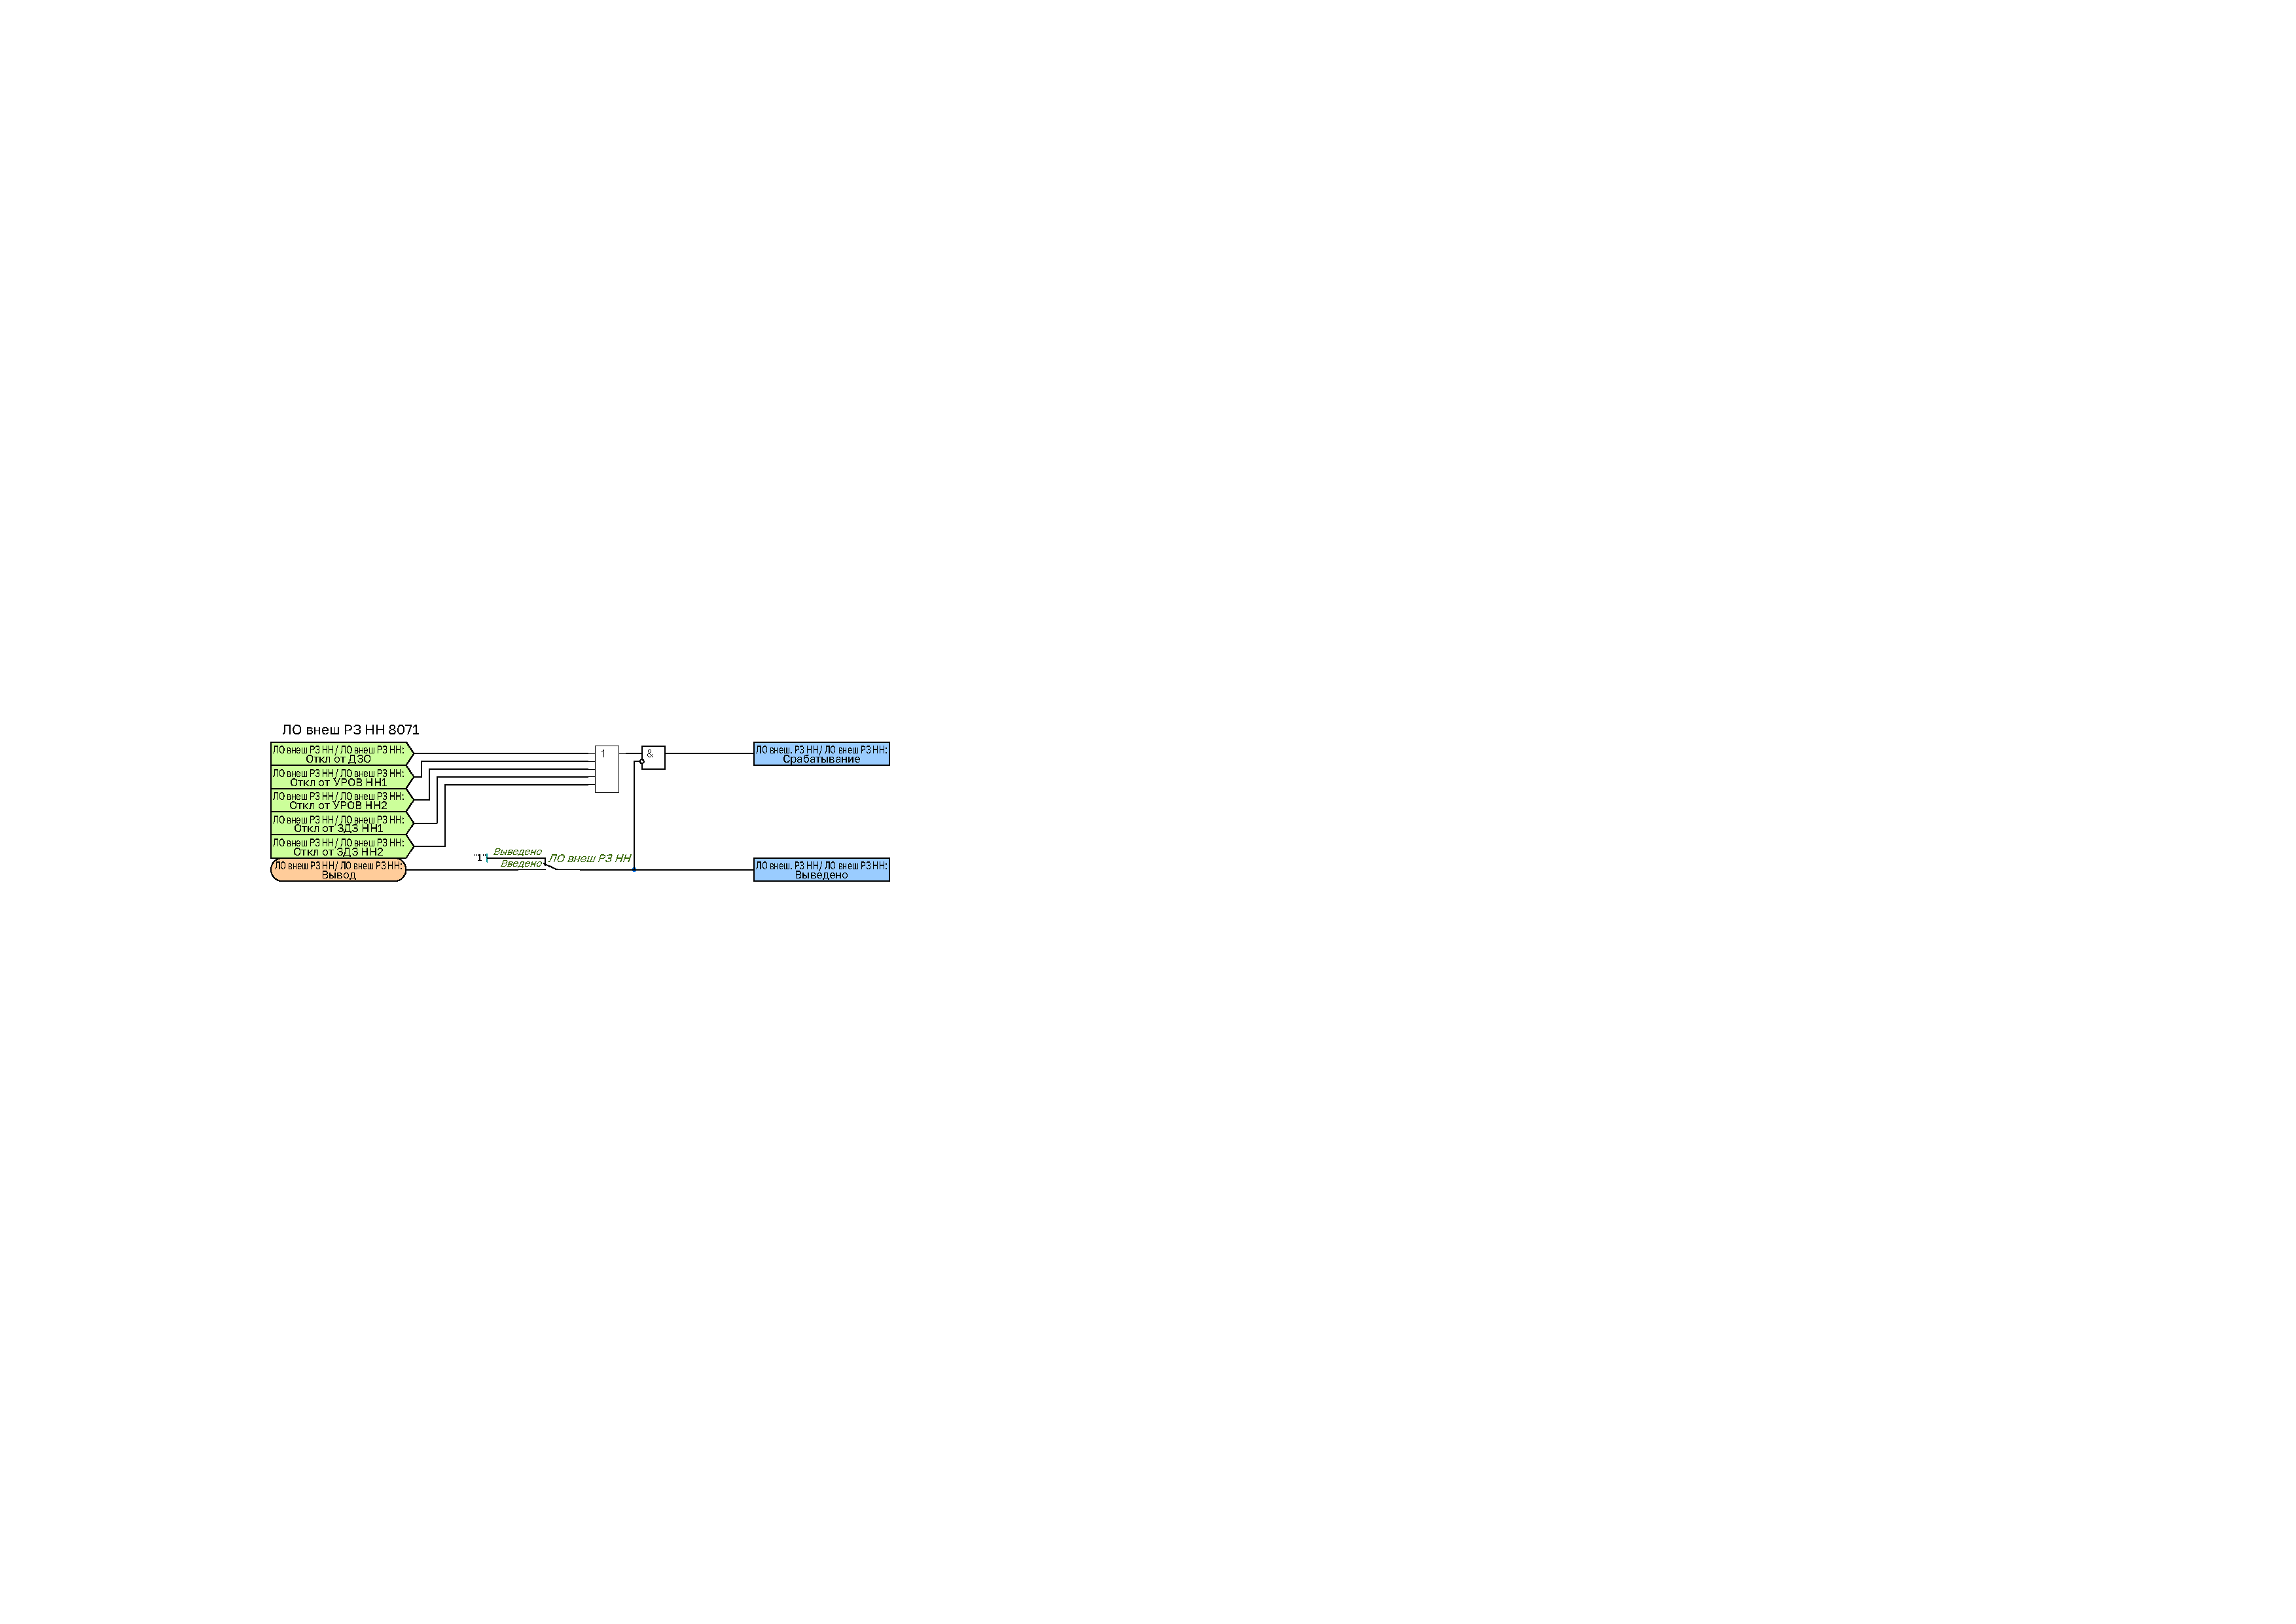
\includegraphics[width=1\textwidth,height=1\textheight,keepaspectratio]{img40.pdf}
\captionof{figure}{Функциональная схема логики внешних отключений НН}\label{pic:LO_NN}
\end{figure}

\item
Уставки ЛО внеш НН приведены в таблице \ref{app_set:lovneshnn}.


\item
Логика внешний отключений РЗ АПТ выводится накладками \textbf{«ЛО внеш АПТ»}.

\item
Команда на срабатывание \textit{«СР. ЛО внеш АПТ»} формируются при возникновении одного из следующих событий:
\begin{itemize}
\item Откл. от АПТ;
\item Откл. от ШАОТ.
\end{itemize}

\vspace{2mm}
\begin{figure}[H]
\centering
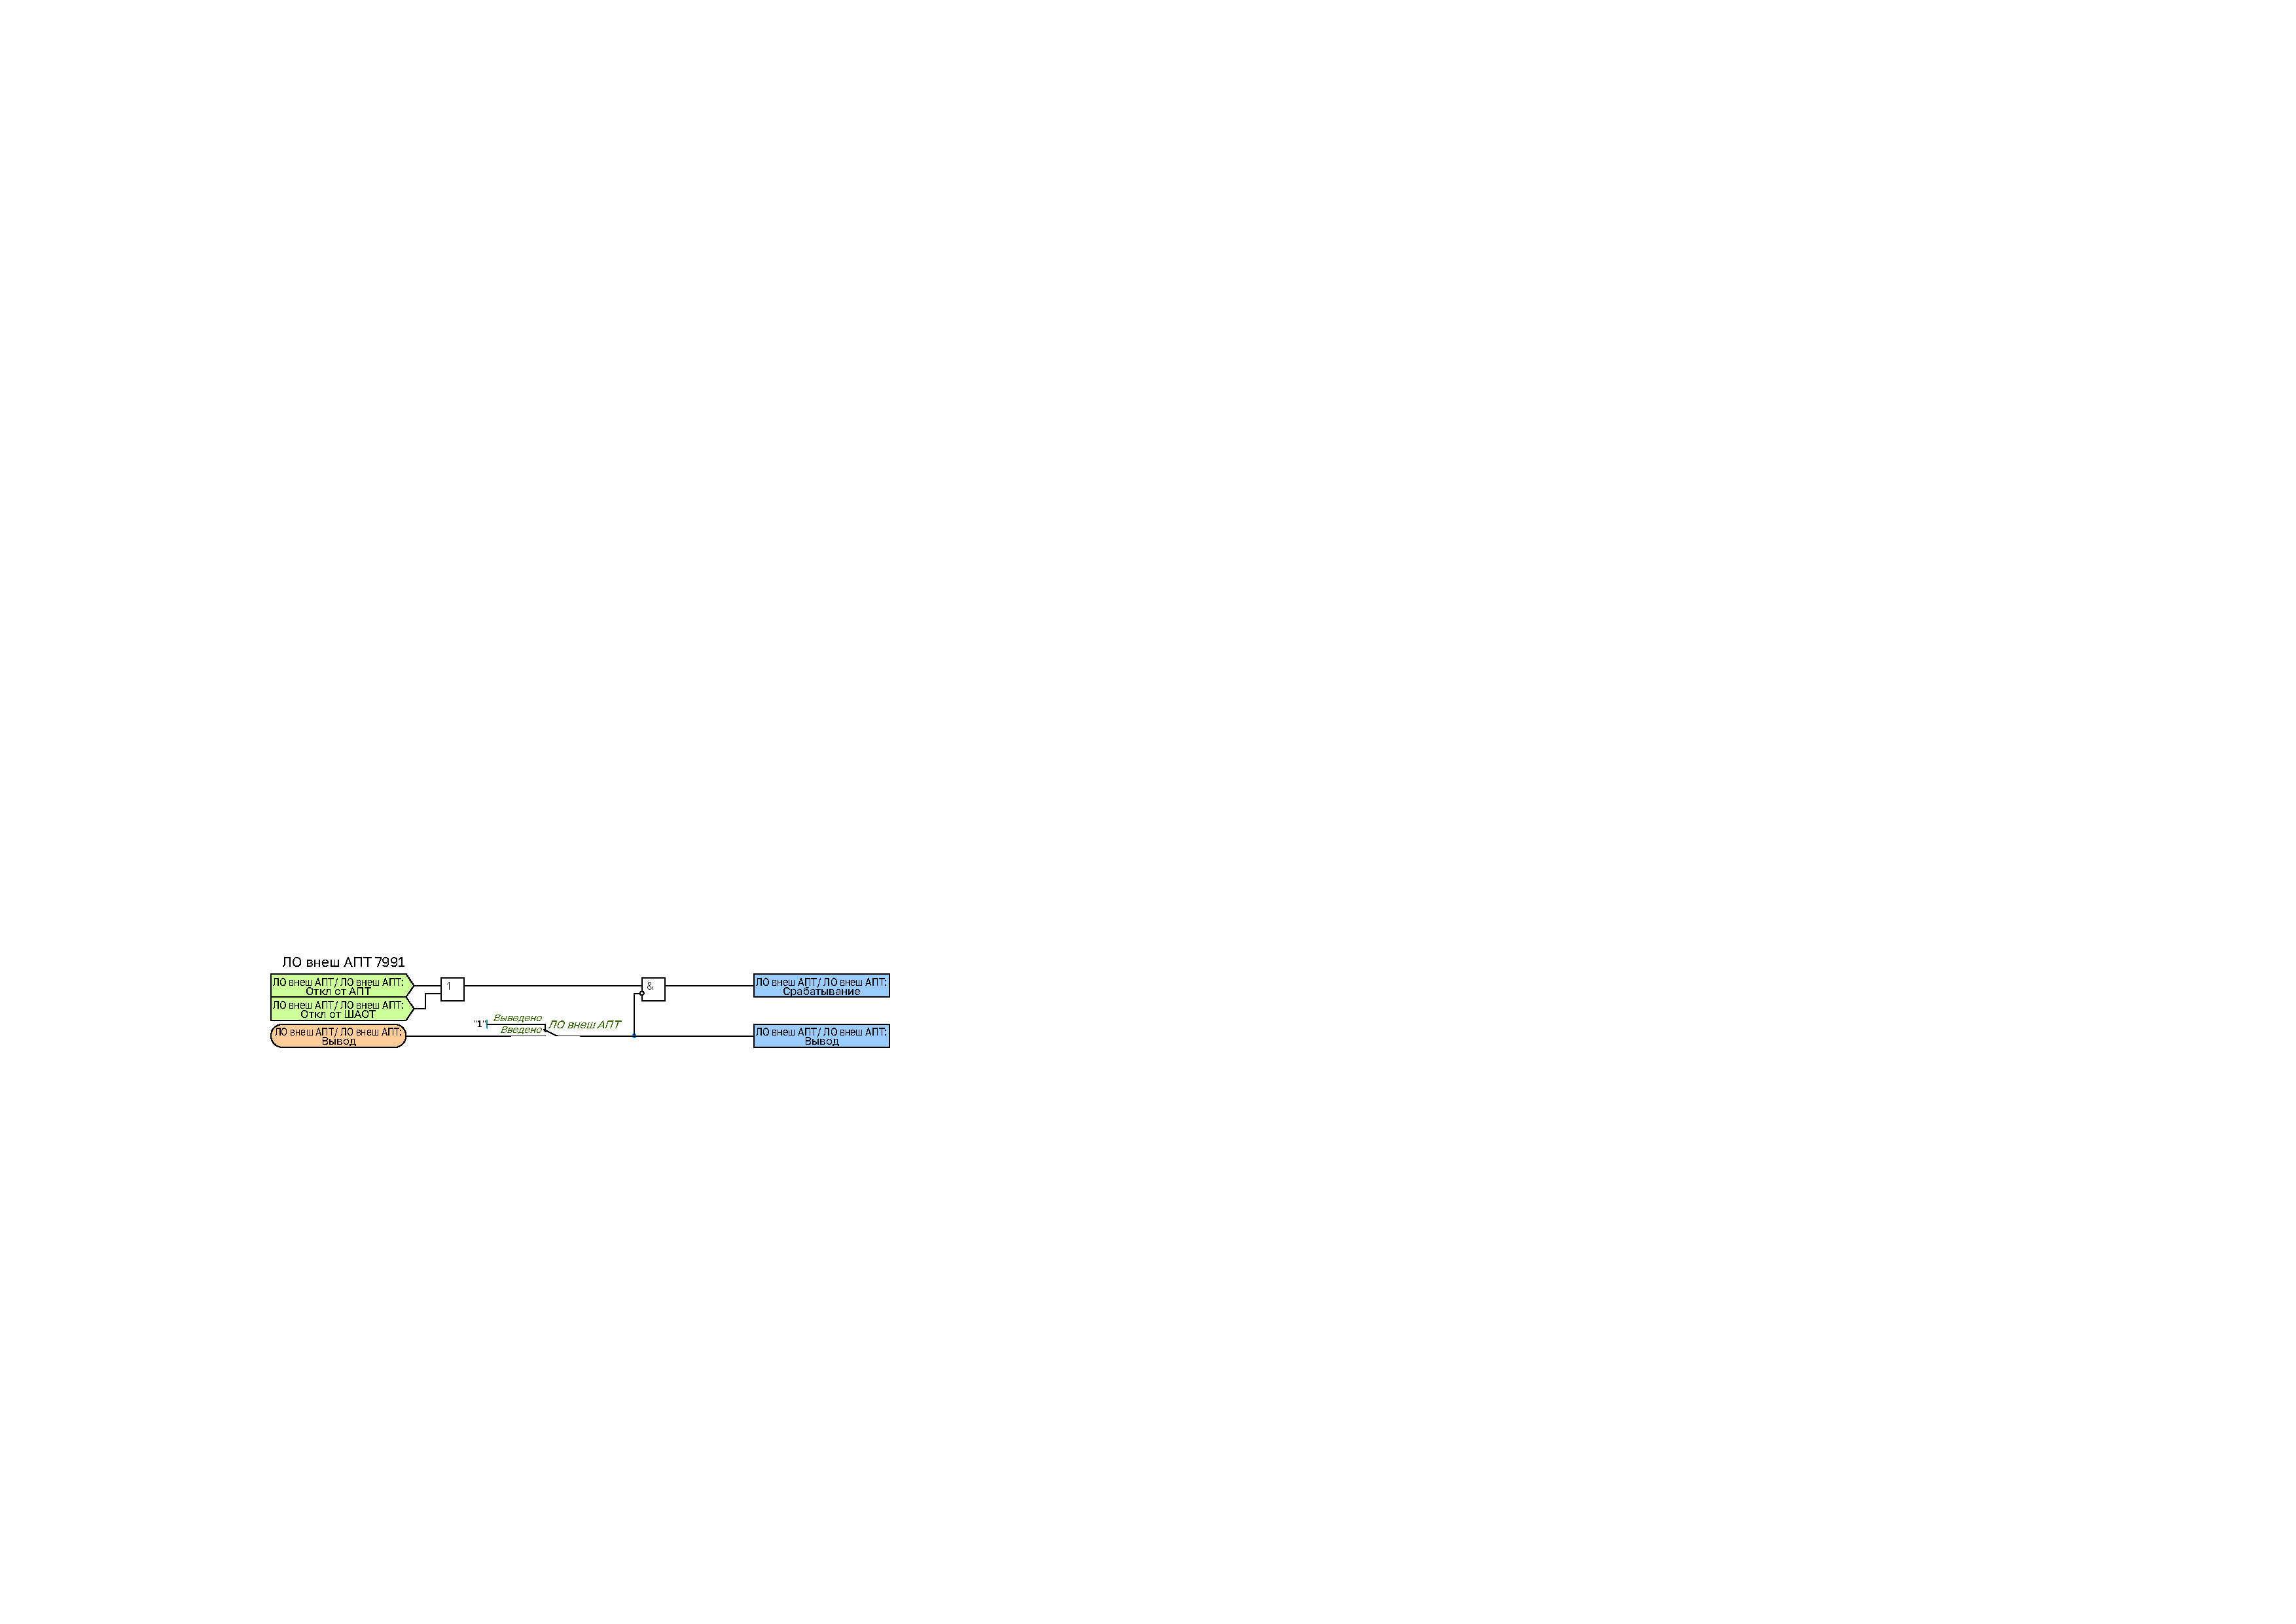
\includegraphics[width=1\textwidth,height=1\textheight,keepaspectratio]{img41.pdf}
\captionof{figure}{Функциональная схема логики внешних отключений АПТ}\label{pic:LO_APT}
\end{figure}

\item
Уставки ЛО внеш АПТ приведены в таблице \ref{app_set:lovneshapt}.

\end{enumerate}\color{unidarkgreen}{\subsection{Логика отключения общая}}
\color{black}

\begin{enumerate}[label=\arabic{section}.\arabic{subsection}.\arabic*,  align=left, labelsep=4pt, leftmargin=0pt, itemindent=57pt]

\item
Срабатывание логики отключения основных защит формируются при включенной накладке \textbf{«ЛО осн»} следующими сигналами:
\begin{itemize}
\item Откл.ДТЗ;
\item Отключение от ГЗ АТ сигн;
\item Ср. ГЗ АТ откл;
\item Ср. ГЗ РПН;
\item Отключение от ГЗ ЛРТ сигн;
\item Ср. ГЗ ЛРТ откл;
\item Ср.отсеч.клап. АТ;
\item Ср.предохр.клап. АТ;
\item Ср.предохр.клап. ЛРТ;
\item Откл. от ТЗ АТ;
\item Откл. от ТЗ ЛРТ;
\item Ср. ЗПО.
\end{itemize}

\item
Логика деления от МТЗ-1 НН1(НН) выводится накладкой \textbf{«ЛД НН от МТЗ-1 НН»}. Срабатывание логики деления формируются при возникновении пуска МТЗ-1 НН. Так же срабатывание контролируется выдержкой времени \textbf{«Тср МТЗ-1 на В НН»}.

\item
Логика деления от МТЗ-2 НН1 выводится накладкой \textbf{«ЛД НН2 от МТЗ-2 НН»}. Срабатывание логики деления формируются при возникновении пуска МТЗ-2 НН. Так же срабатывание контролируется выдержкой времени \textbf{«Тср МТЗ-2 на В НН»}.

\item
Уставки ЛД НН приведены в таблице \ref{app_set:ldnn}.

\item
Действие основных защит на отсечной клапан вводится накладкой \textbf{«Действие на ОК»}, время импульса действия регулируется \textbf{«Tимп ОК»}.

\item
Уставки ЛО ОК приведены в таблице \ref{app_set:look}.


\begin{figure}[H]
\centering
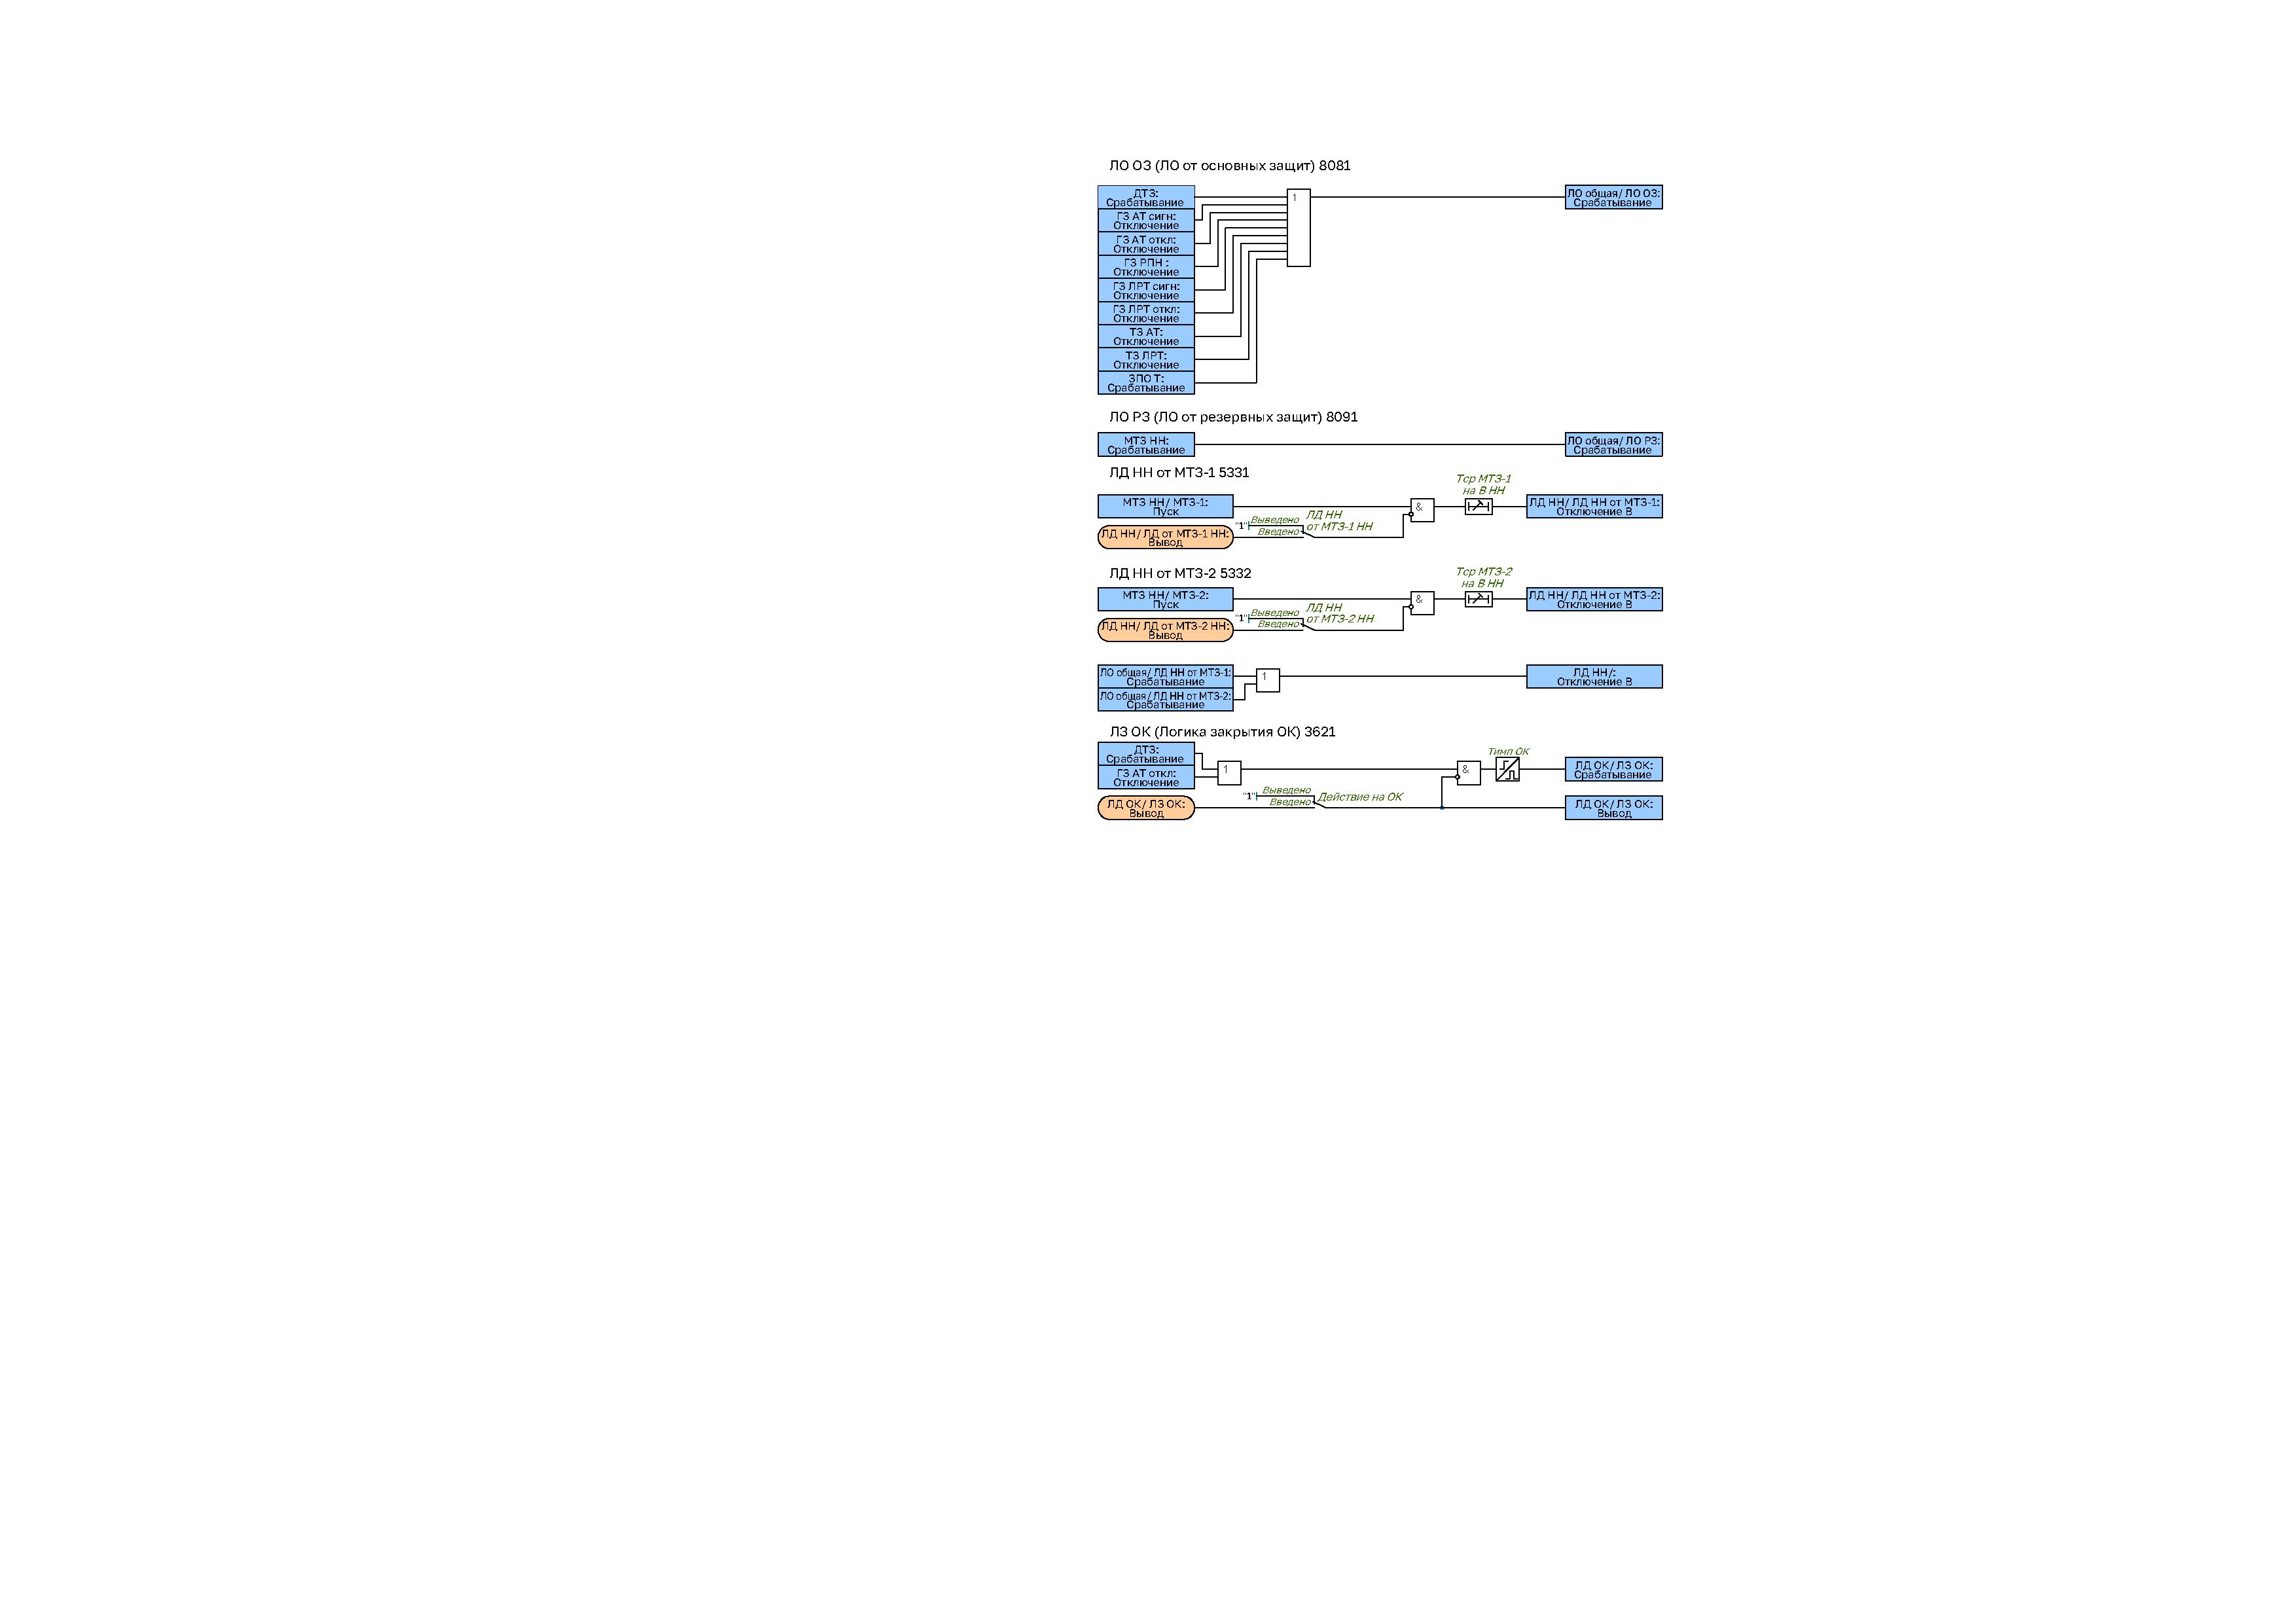
\includegraphics[width=0.9\textwidth,height=0.9\textheight,keepaspectratio]{img42.pdf}
\captionof{figure}{Функциональная схема общей логики отключения}\label{pic:LO_gen}
\end{figure}


\end{enumerate}\color{unidarkgreen}{\subsection{Логика отключения выключателей сторон ВН и СН}}
\color{black}

\begin{enumerate}[label=\arabic{section}.\arabic{subsection}.\arabic*,  align=left, labelsep=4pt, leftmargin=0pt, itemindent=57pt]

\item
Логика отключения В1(ЛВ)ВН выводится накладкой \textbf{«ЛО В1(ЛВ)ВН»}. 

\item
На отключение В1(ЛВ)ВН формируются при возникновении одного из следующих событий:
\begin{itemize}
\item ЛО осн. РЗ;
\item ЛО рез. РЗ;
\item ЛО внеш РЗ ВН;
\item ЛО внеш АПТ;
\item ТЗО СН (ТЗО-ф);
\item ТЗО СН (ТЗО-н);
\item ЛО внеш РЗ ВН;
\item ЛО внеш РЗ СН.
\end{itemize}

\item
Запрет АПВ формируются при возникновении одного из следующих событий:
\begin{itemize}
\item ЗАПВ внеш РЗ ВН;
\item ЗАПВ внеш РЗ СН.
\end{itemize}

\item
Пуск УРОВ НН формируется сигналом \textbf{«Ср. ПО УРОВ НН»}.

\item
Алгоритм работы логики отключения В1(ЛВ) ВН приведен на рисунке \ref{pic:LO_Q1_LV_VN}. Алгоритмы работы логики отключения В2(ОВ) ВН, В3 ВН, В4 ВН выполнены аналогично. Уставки ЛО выключателей стороны ВН приведены в таблицах \ref{app_set:lovvn1}-\ref{app_set:lovvn4}.

\begin{figure}[H]
\centering
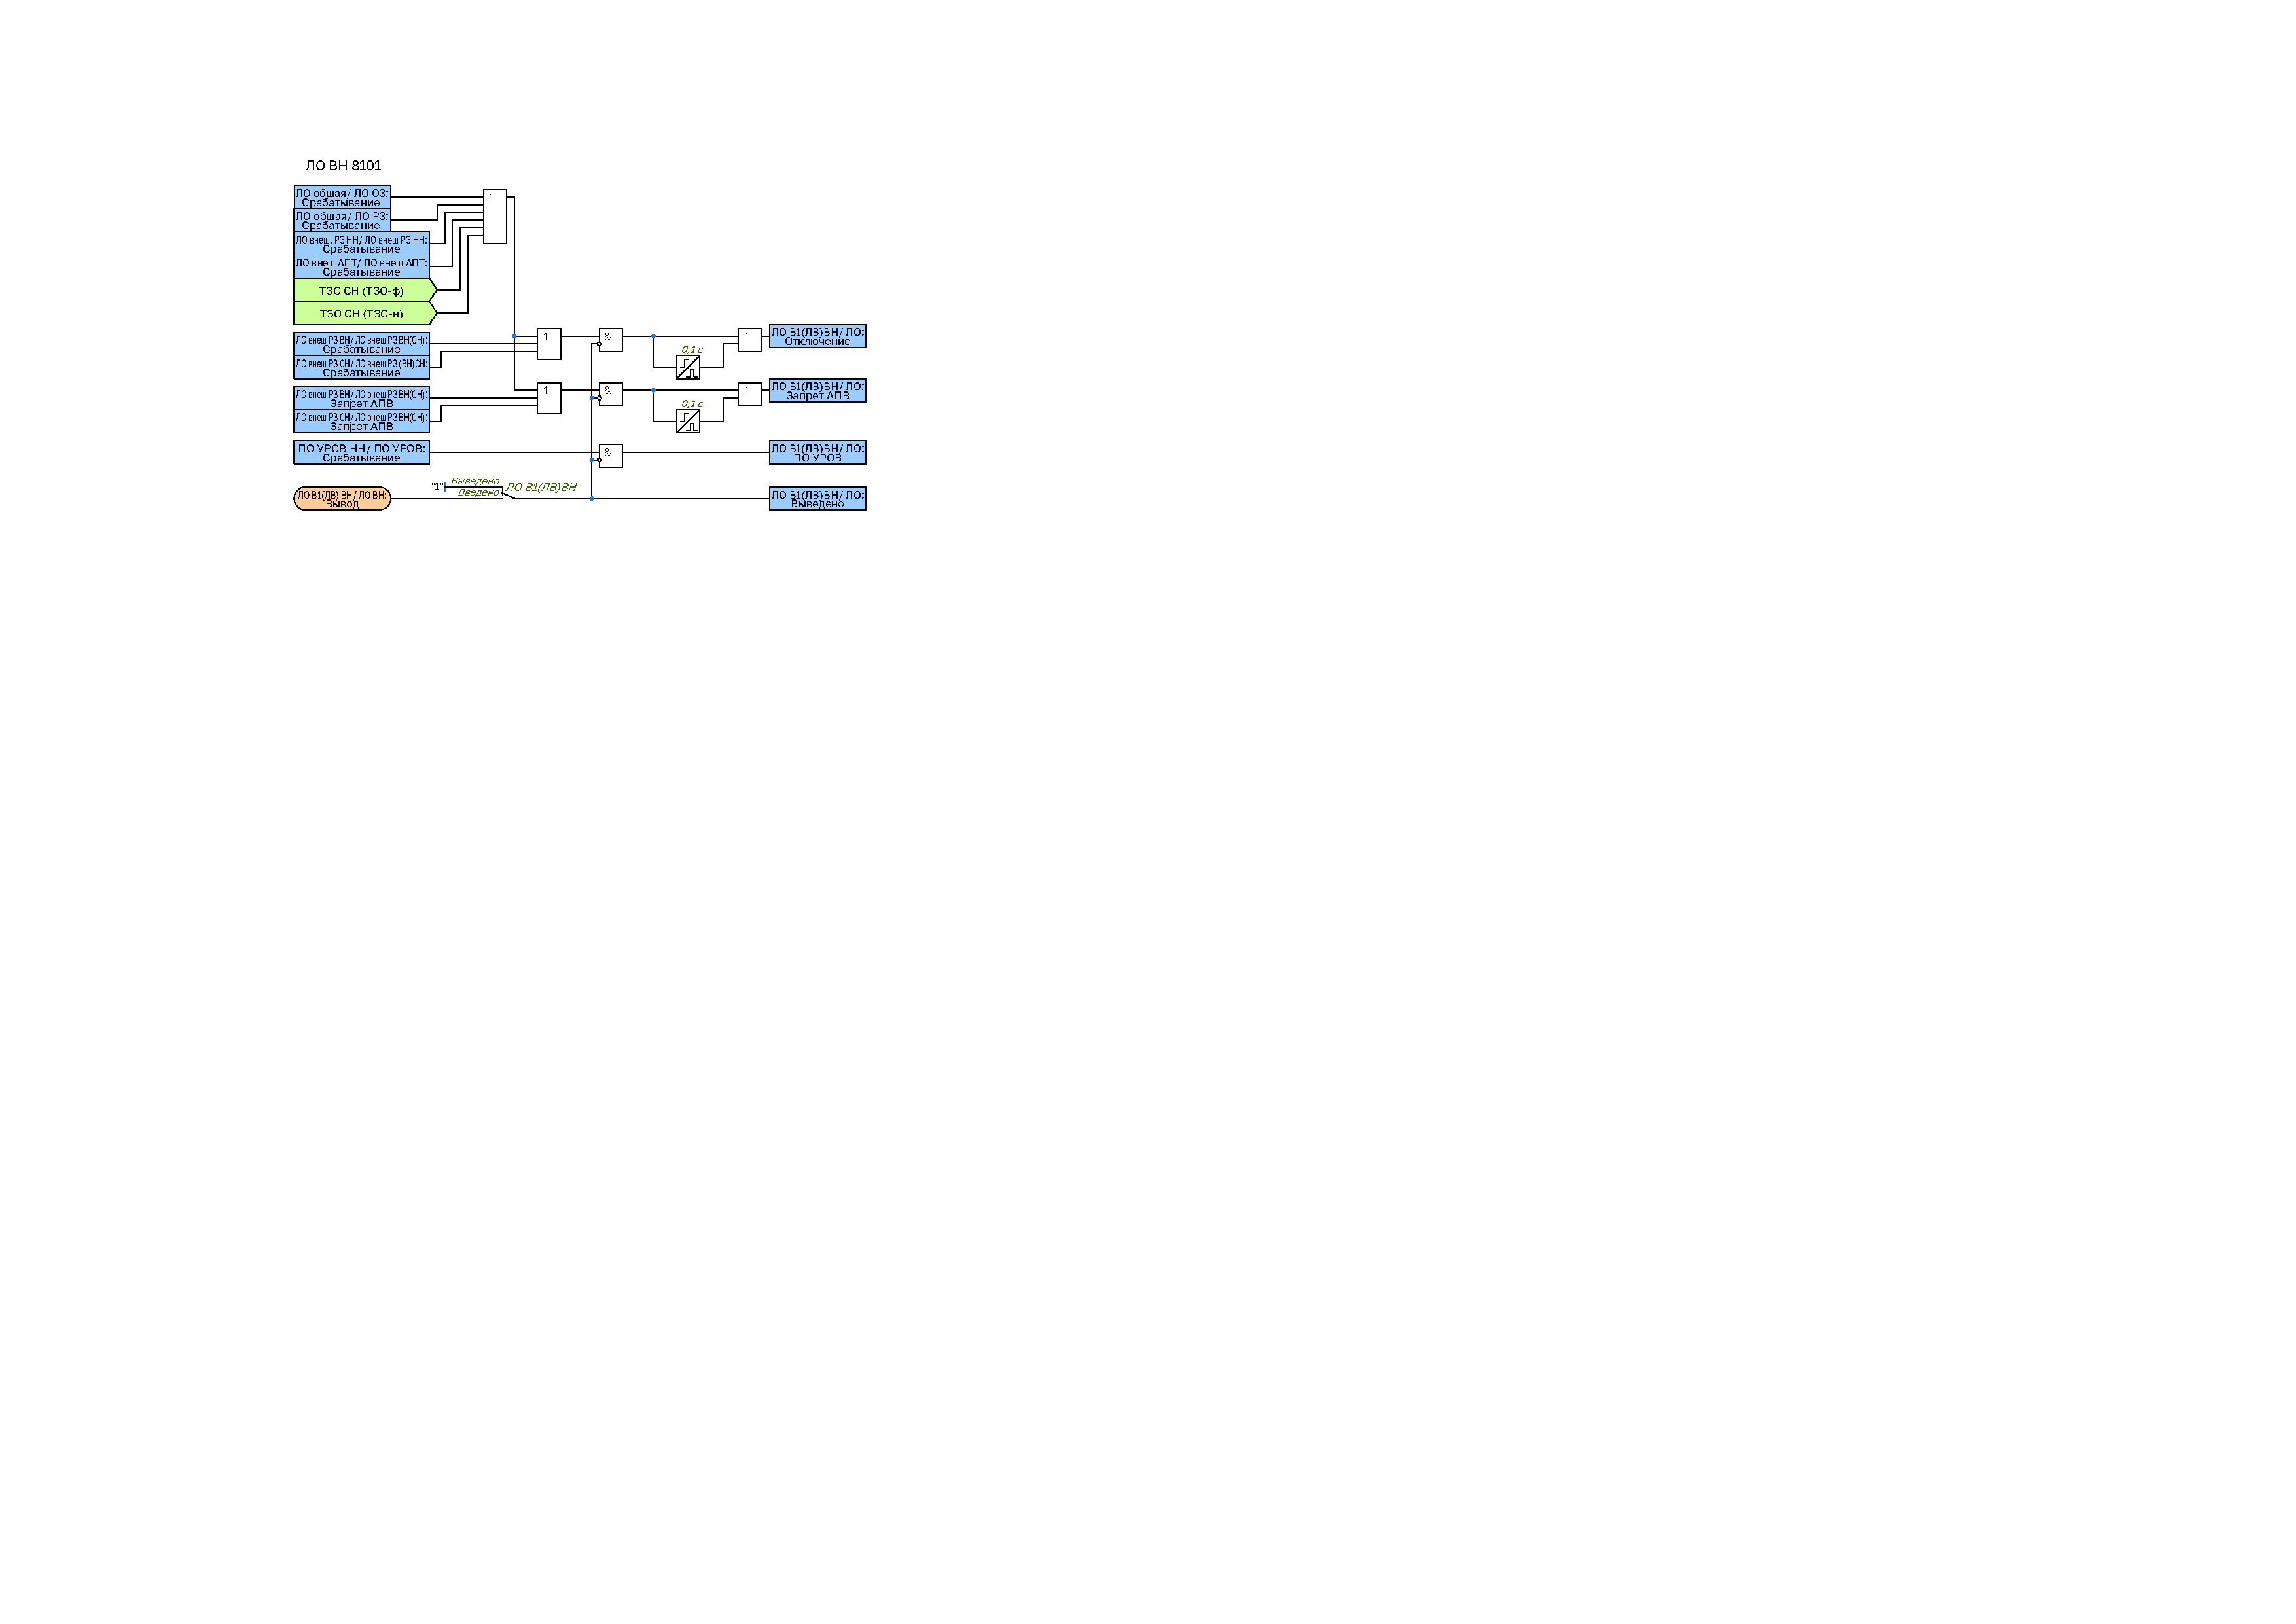
\includegraphics[width=1\textwidth,height=1\textheight,keepaspectratio]{img43.pdf}
\captionof{figure}{Функциональная схема логики отключения В1(ЛВ) ВН}\label{pic:LO_Q1_LV_VN}
\end{figure}

\item
Логика отключения В1(ЛВ) СН выводится накладкой \textbf{«ЛО В1(ЛВ)СН»}. 

\item
На отключение В1(ЛВ) СН формируются при возникновении одного из следующих событий:
\begin{itemize}
\item ЛО осн. РЗ;
\item ЛО рез. РЗ;
\item ЛО внеш РЗ ВН;
\item ЛО внеш АПТ;
\item ТЗО ВН (ТЗО-ф);
\item ТЗО ВН (ТЗО-н);
\item ЛО внеш РЗ ВН;
\item ЛО внеш РЗ СН.
\end{itemize}

\item
Запрет АПВ формируются при возникновении одного из следующих событий:
\begin{itemize}
\item ЗАПВ внеш РЗ ВН;
\item ЗАПВ внеш РЗ СН.
\end{itemize}

\item
Пуск УРОВ НН формируется сигналом \textbf{«Ср. ПО УРОВ НН»}.

\item
Алгоритм работы логики отключения В1(ЛВ) СН приведен на рисунке \ref{pic:LO_Q1_LV_VN}. Алгоритм работы логики отключения В2(ОВ) СН выполнен аналогично. Уставки ЛО выключателей стороны СН приведены в таблицах \ref{app_set:lovsn1}, \ref{app_set:lovsn2}.

\begin{figure}[H]
\centering
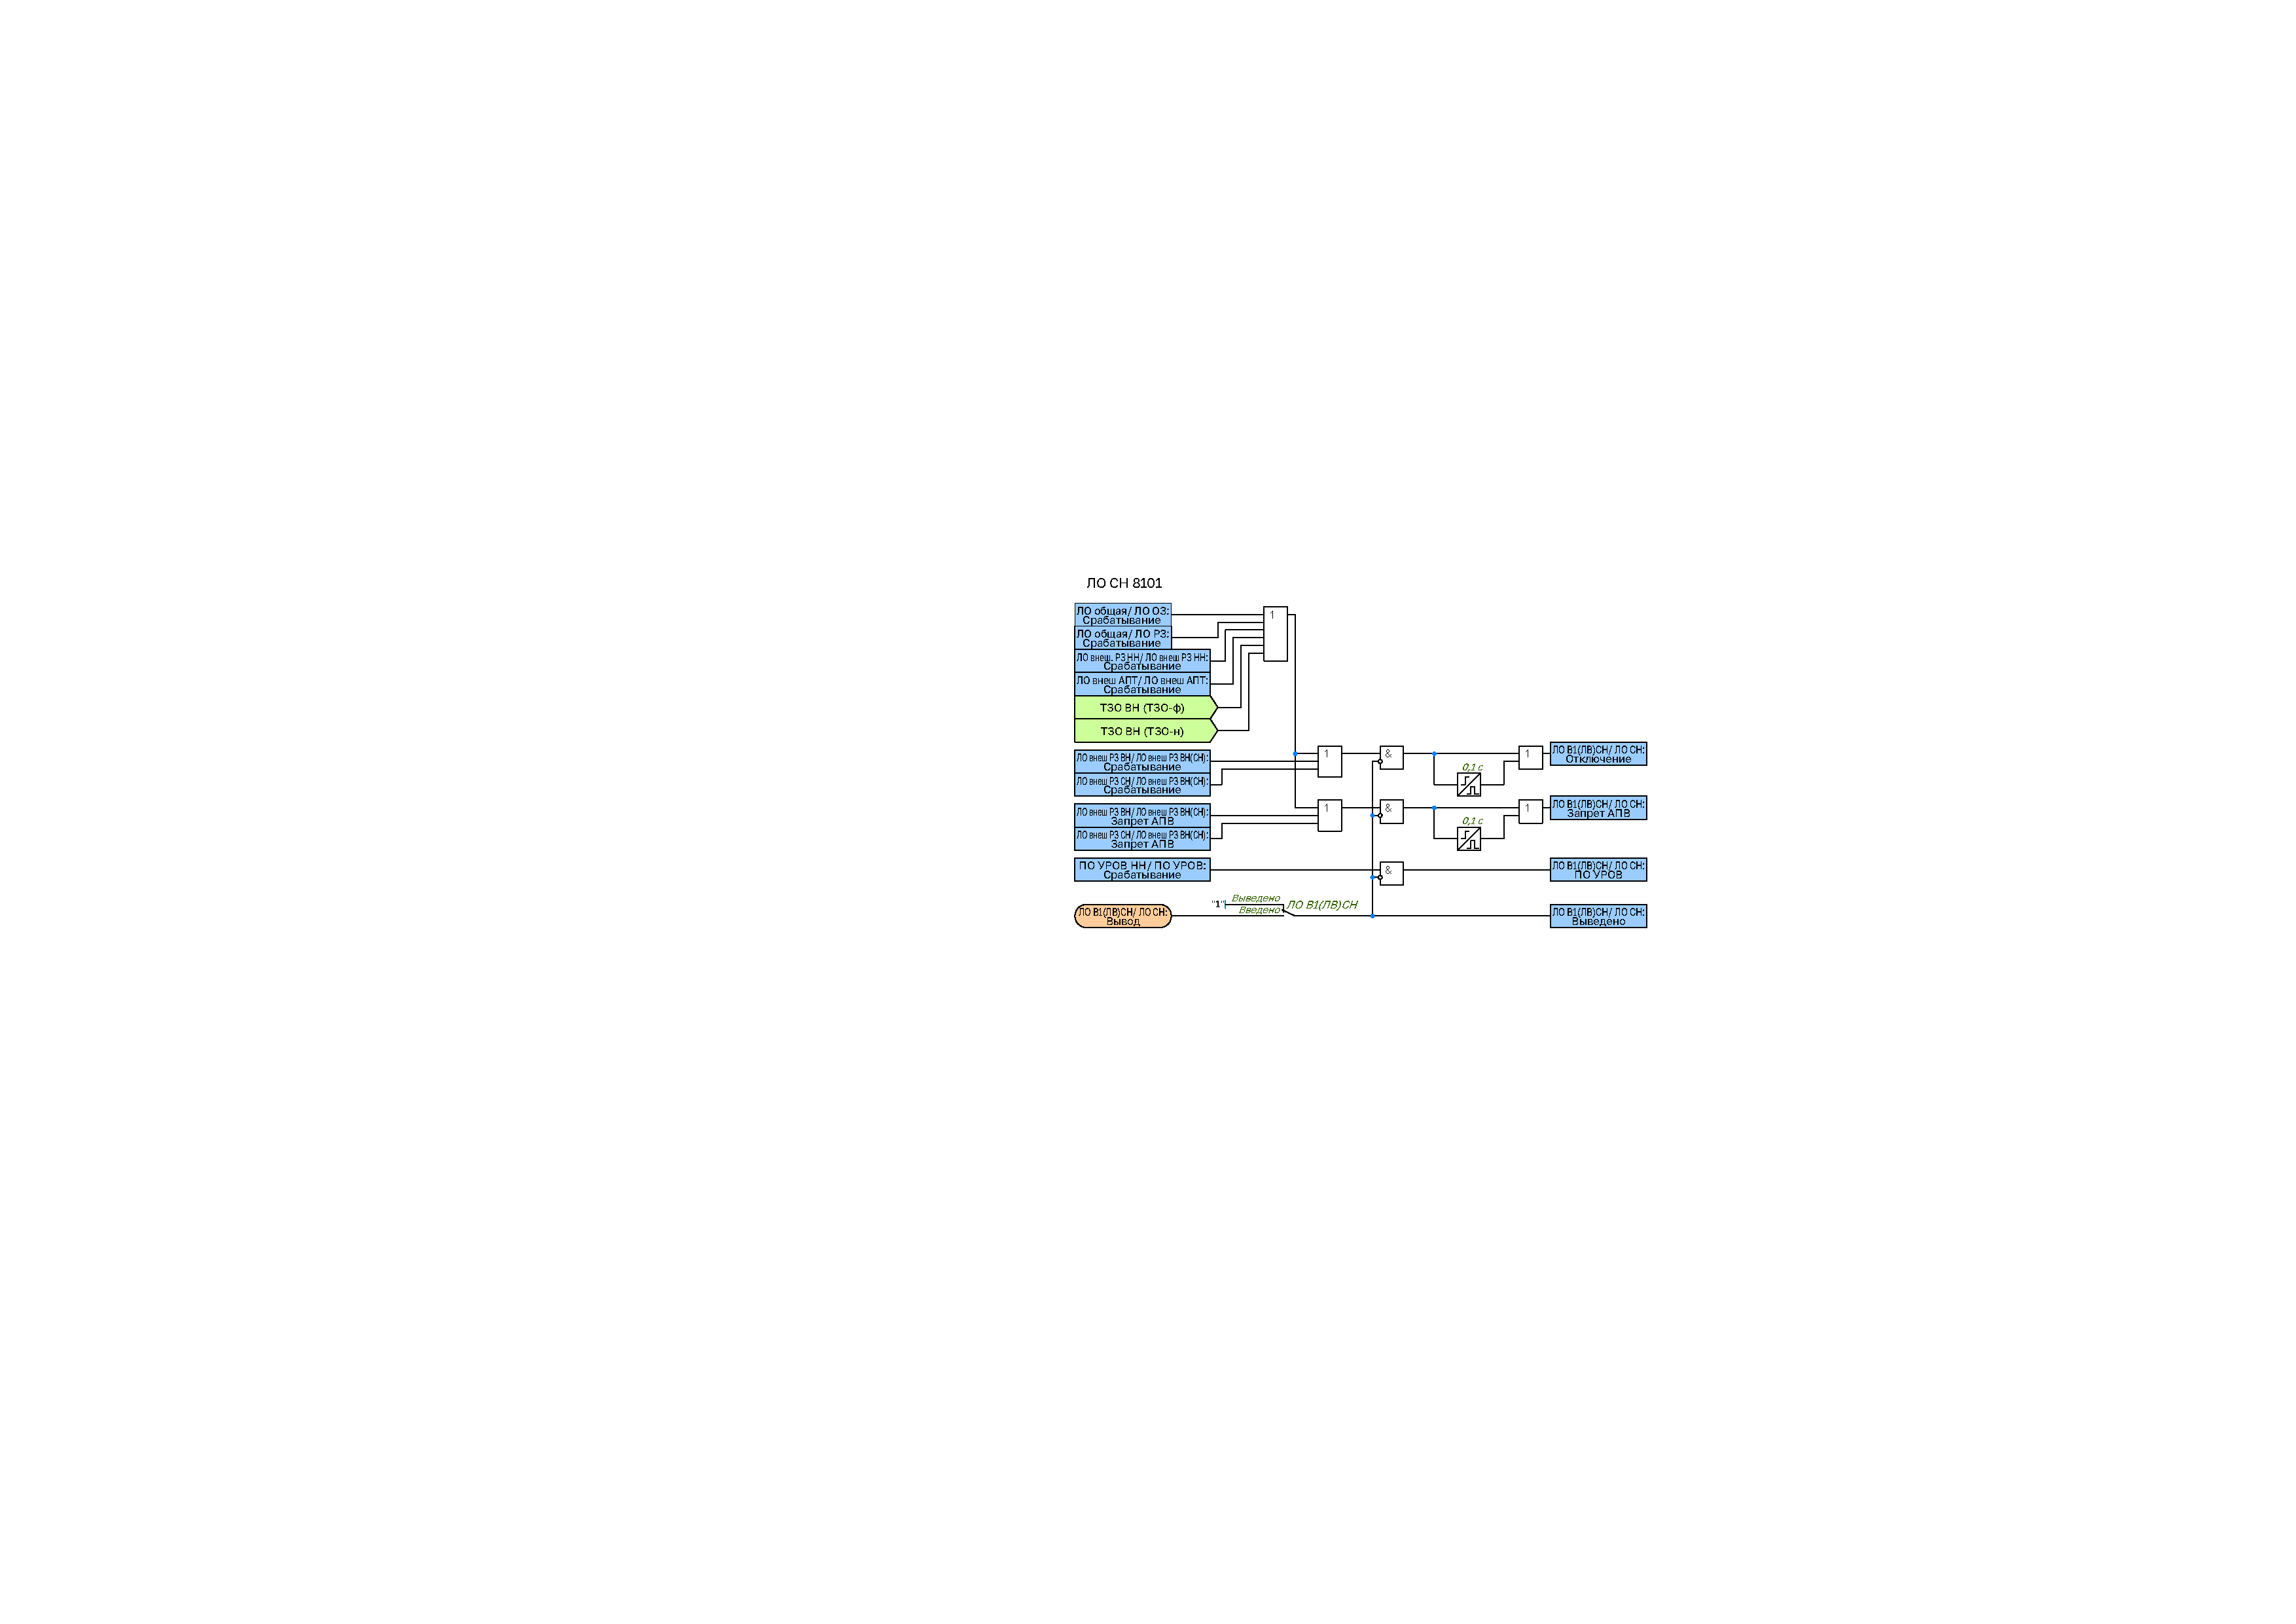
\includegraphics[width=1\textwidth,height=1\textheight,keepaspectratio]{img44.pdf}
\captionof{figure}{Функциональная схема логики отключения В1(ЛВ) СН}\label{pic:LO_Q1_LV_SN}
\end{figure}













\end{enumerate}\color{unidarkgreen}{\subsection{Логика отключения выключателей стороны НН}}
\color{black}

\begin{enumerate}[label=\arabic{section}.\arabic{subsection}.\arabic*,  align=left, labelsep=4pt, leftmargin=0pt, itemindent=57pt]

\item
Логика отключения В НН1 выводится накладкой \textbf{«ЛО НН1»}. 

\item
Цепь отключения В НН1 выводится накладкой \textbf{«ЦО В НН1»}. Время возврата импульса на отключение регулируется уставкой \textbf{«Tвозвр откл НН1»}. На отключение В1(ЛВ) формируется при возникновении одного из следующих событий:
\begin{itemize}
\item ЛО осн. РЗ;
\item ЛО рез. РЗ;
\item ЛО внеш АПТ;
\item ТЗО СН (ТЗО-ф);
\item ТЗО СН (ТЗО-н);
\item ТЗО ВН (ТЗО-ф);
\item ТЗО ВН (ТЗО-н);
\item ЛО внеш РЗ ВН;
\item ЛО внеш РЗ СН;
\item ЛО внеш РЗ НН.
\end{itemize}

\item
Запрет АПВ формируются при возникновении одного из следующих событий:
\begin{itemize}
\item ЗАПВ внеш РЗ ВН;
\item ЗАПВ внеш РЗ СН.
\end{itemize}

\item
\textcolor{red}{Запрет АВР НН1 формируется при появлении сигнала \textbf{«Ср. МТЗ-2 НН»}.}

\item
Алгоритм работы логики отключения В НН1 приведен на рисунке \ref{pic:LO_Q1_NN}. Алгоритм работы логики отключения В НН2 выполнен аналогично. Уставки ЛО выключателей стороны НН приведены в таблицах \ref{app_set:lovnn1}, \ref{app_set:lovnn2}.


\begin{figure}[H]
\centering
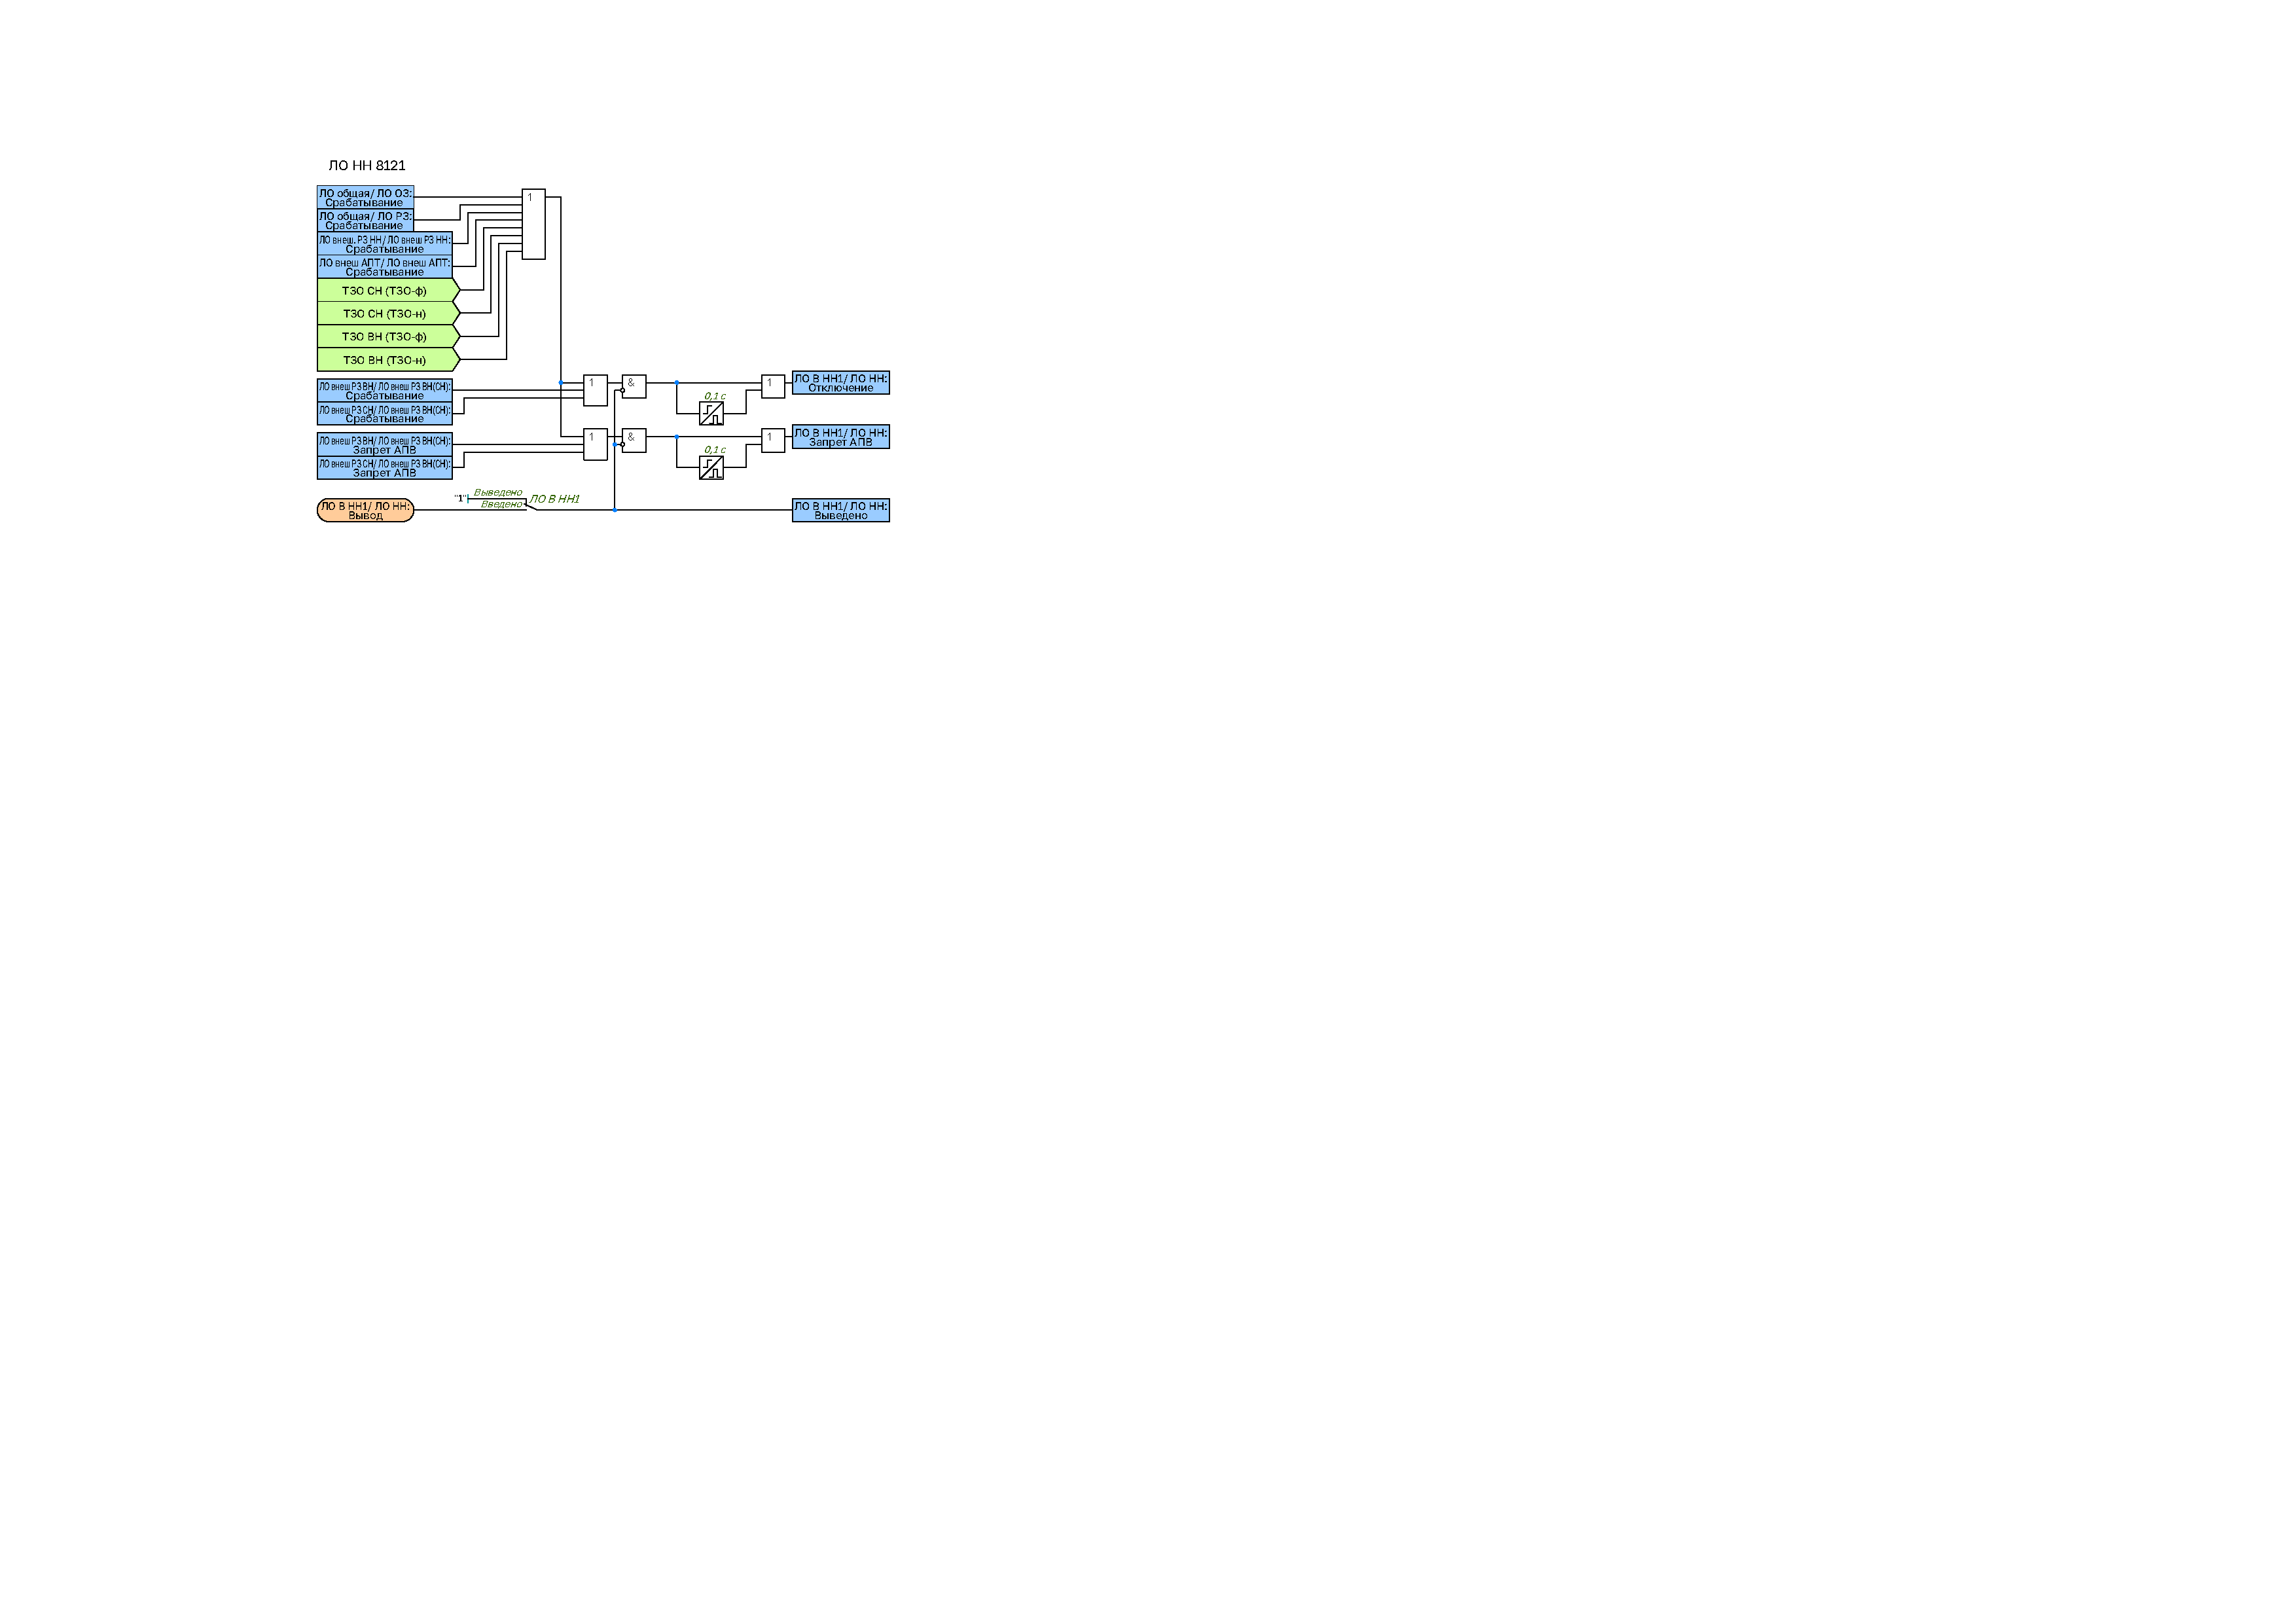
\includegraphics[width=1\textwidth,height=1\textheight,keepaspectratio]{img45.pdf}
\captionof{figure}{Функциональная схема логики отключения В НН1}\label{pic:LO_Q1_NN}
\end{figure}

\end{enumerate}
\color{unidarkgreen}{\subsection{Фиксация положения выключателей}}
\color{black}

\begin{enumerate}

\item
Функциональный блок фиксации положения выключателей (ФПВ) предназначен для определения состояния выключателей на основании технологической информации:

\begin{itemize}
    \item состояния блок-контактов выключателя;
    \item положения разъединителей в цепи выключателя;
    \item информации о выводе в ремонт выключателя.
\end{itemize}

\def\Qone{Не определено}
\def\Qtwo{Не определено}

\ifbool{isLV}{
\def\Qone{В1} 
\def\Qtwo{В2} 
}{}

\ifbool{isDZAT}{
\def\Qone{В1(ЛВ) ВН} 
\def\Qtwo{В2(ОВ) ВН} 
}{}

\ifbool{isLV}{
\item
Контроль положения разъединителей при формировании сигналов включенного или отключенного положения выключателей (например, \textit{«В1 включен»} и \textit{«В2 отключен»} для выключателя В1) вводится программным ключом \textbf{«Контр. Р В1»}. Также имеется возможность выбрать количество разъединителей, участвующих в формировании сигналов включенного или отключенного положения выключателей, для выключателя В1 она задается программным переключателем \textbf{«Схема Р В1»}.
\item
Также функция ФПВ пофазно контролирует состояние блок-контактов выключателя и в случае расхождения полюсов формирует сигнал \textit{«Внутр. пуск. ЗНФ В1»}.
\item
Функциональная схема логики ФПВ В1 приведена на рисунке \ref{pict_fpv:fpv1}. Уставки ФПВ В1 представлены в таблице \ref{app_set:fpv1}.
}
\ifbool{isDZAT}{
\item
Контроль положения разъединителей при формировании сигналов включенного или отключенного положения выключателей (например, \textit{«В1(ЛВ) ВН включен»} и \textit{«В1(ЛВ) ВН отключен»} для выключателя В1(ЛВ) ВН) вводится программным ключом \textbf{«Контр. Р В1(ЛВ) ВН»}. Также имеется возможность выбрать количество разъединителей, участвующих в формировании сигналов включенного или отключенного положения выключателей, для выключателя В1 она задается программным переключателем \textbf{«Схема Р В1(ЛВ) ВН»}.
\item
Также функция ФПВ пофазно контролирует состояние блок-контактов выключателя и в случае расхождения полюсов формирует сигнал \textit{«Внутр. пуск. ЗНФ В1(ЛВ) ВН»}.
\item
Функциональная схема логики ФПВ В1(ЛВ) ВН приведена на рисунке \ref{pict_fpv:fpv1}. Функциональная схема логики ФПВ В1(ЛВ) СН выполнена аналогично. Уставки ФПВ В1(ЛВ) ВН представлены в таблице \ref{app_set:fpvvn1}. Уставки ФПВ В1(ЛВ) СН представлены в таблице \ref{app_set:fpvsn1}
}


\vspace{2mm}
\begin{figure}[H]
\centering
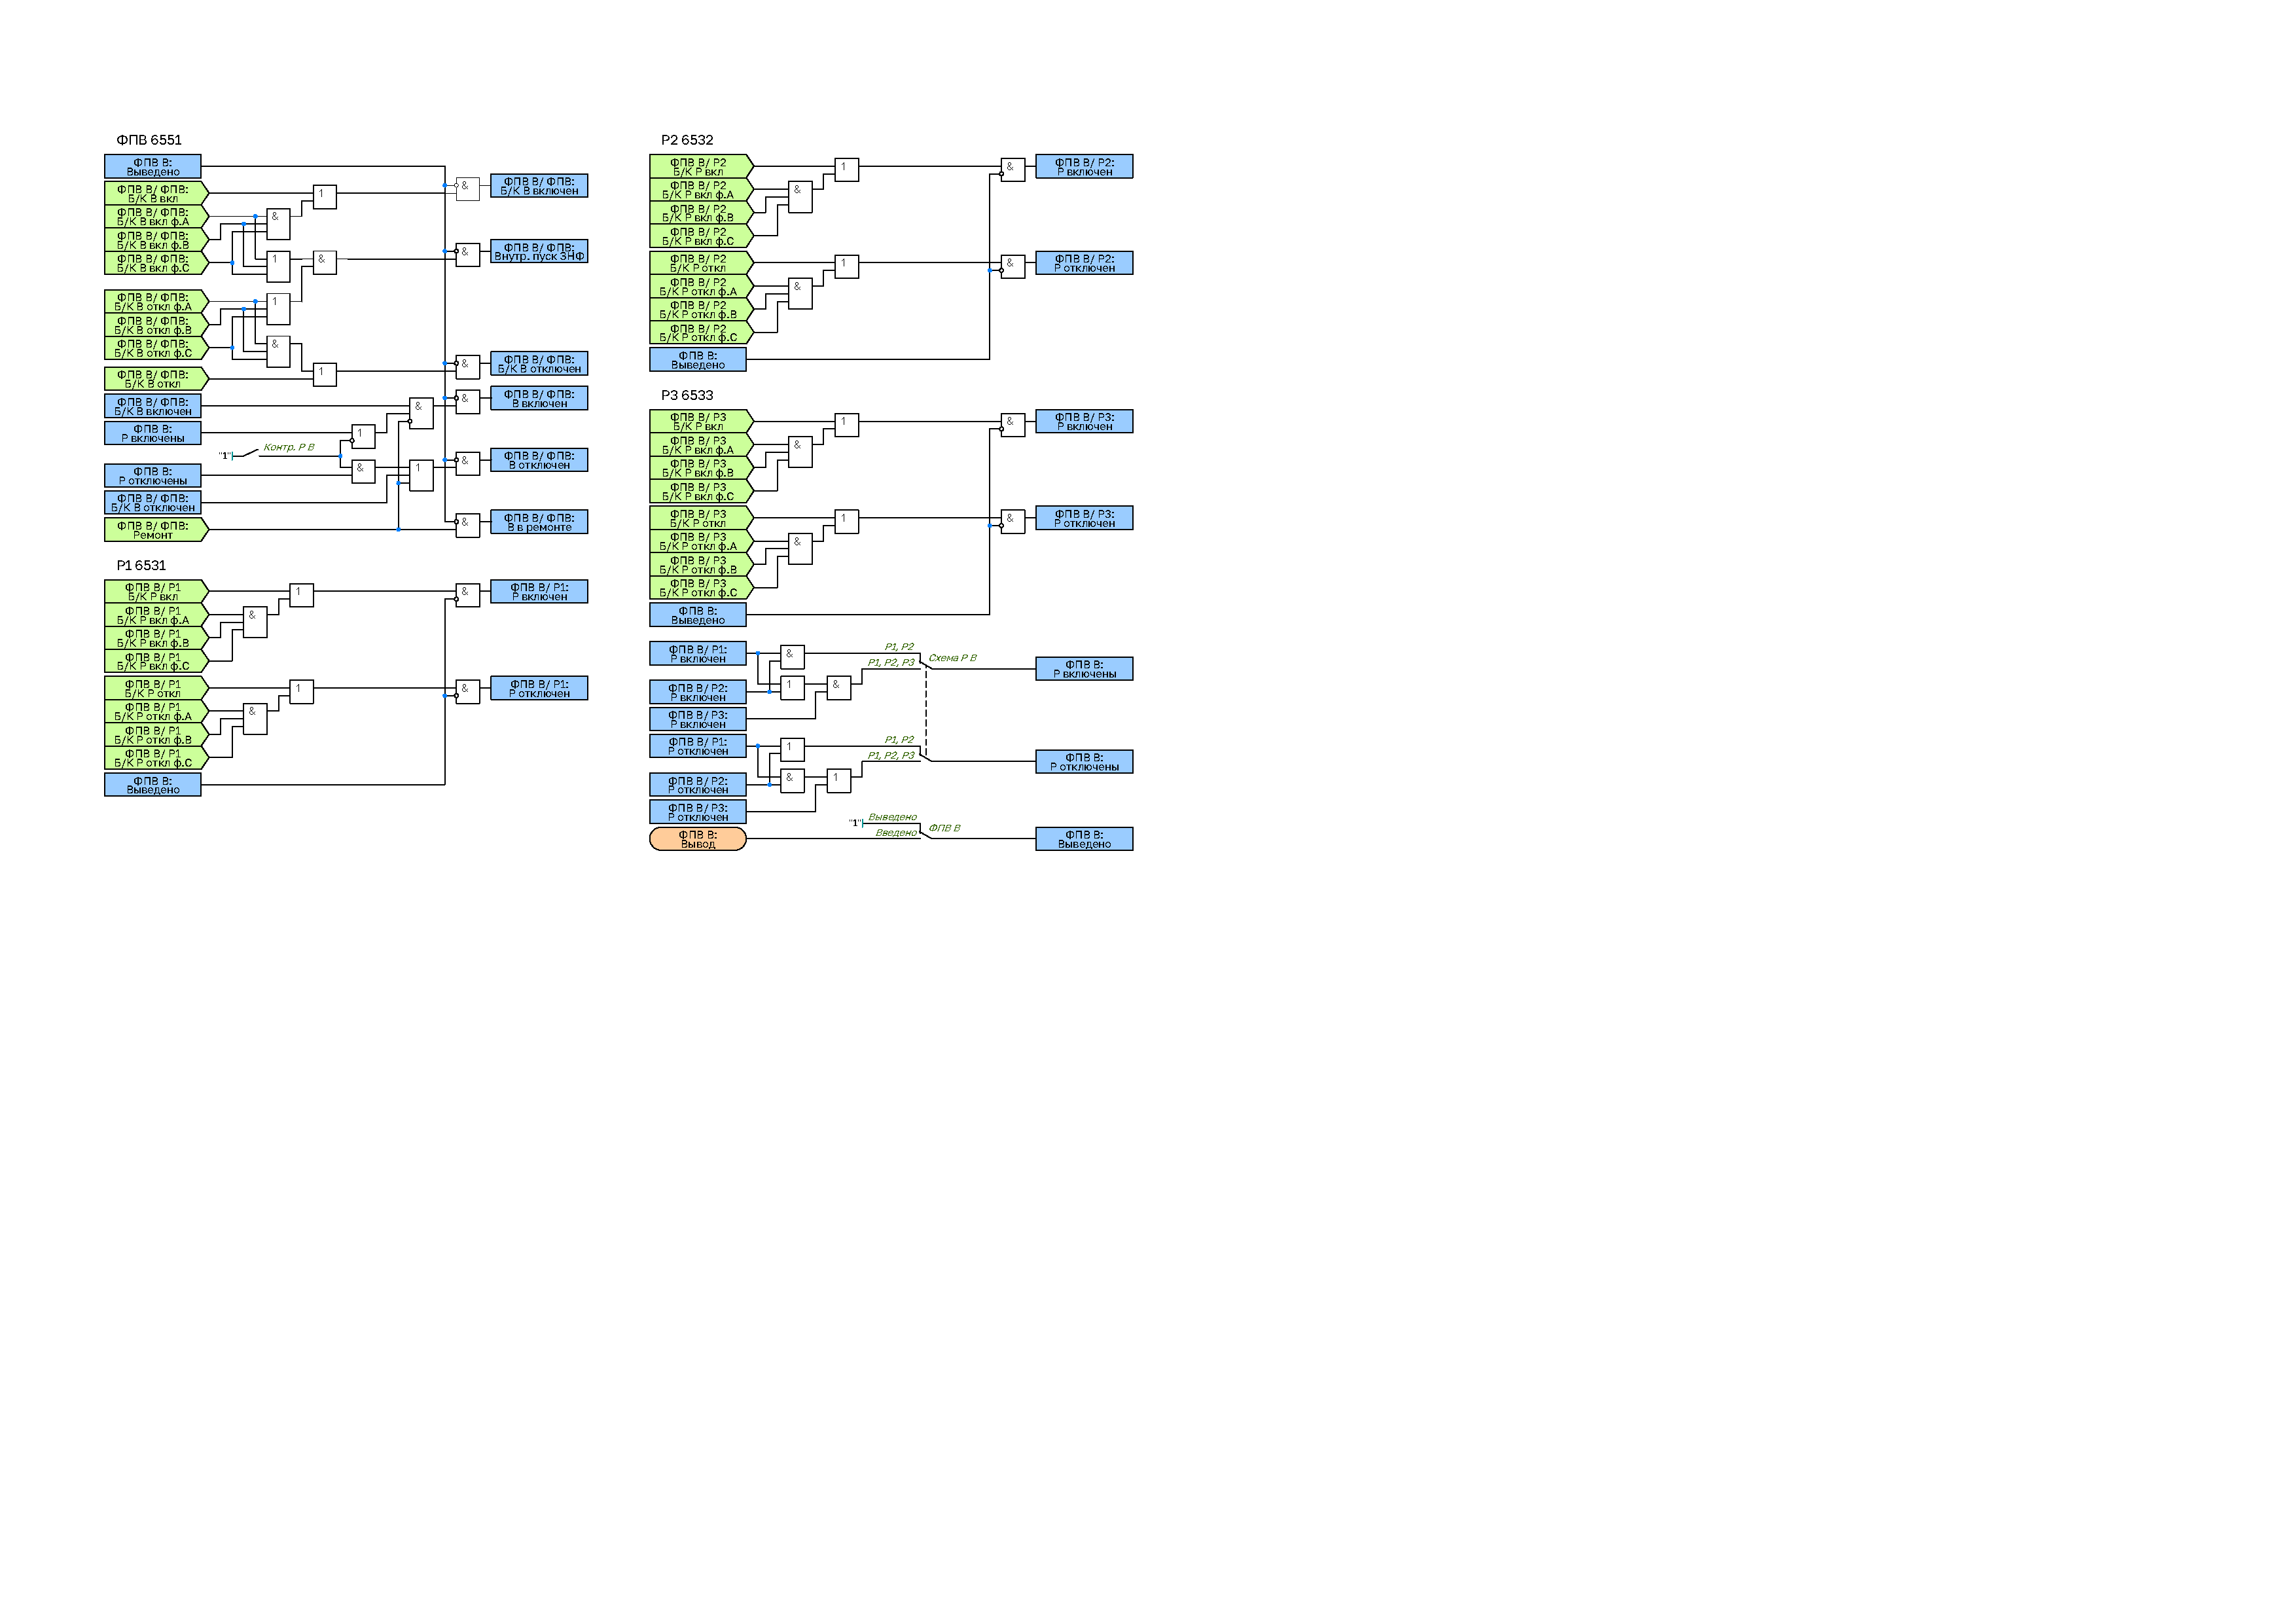
\includegraphics[width=1\textwidth,height=1\textheight,keepaspectratio]{img46.pdf}
\captionof{figure}{Функциональная схема логики ФПВ \Qone}\label{pict_fpv:fpv1}
\end{figure}

\ifbool{isLV}{
\item
Функциональная схема логики ФПВ В2 приведена на рисунке \ref{pict_fpv:fpv2}. Уставки ФПВ В2 представлены в таблице \ref{app_set:fpv2}.
}
\ifbool{isDZAT}{
\item
Функциональная схема логики ФПВ В2(ОВ) ВН приведена на рисунке \ref{pict_fpv:fpv2}. Функциональная схема логики ФПВ В1(ЛВ) СН выполнена аналогично. Уставки ФПВ В2(ОВ) ВН представлены в таблице \ref{app_set:fpvvn2}. Уставки ФПВ В2(ОВ) СН представлены в таблице \ref{app_set:fpvsn2}
}

\vspace{2mm}
\begin{figure}[H]
\centering
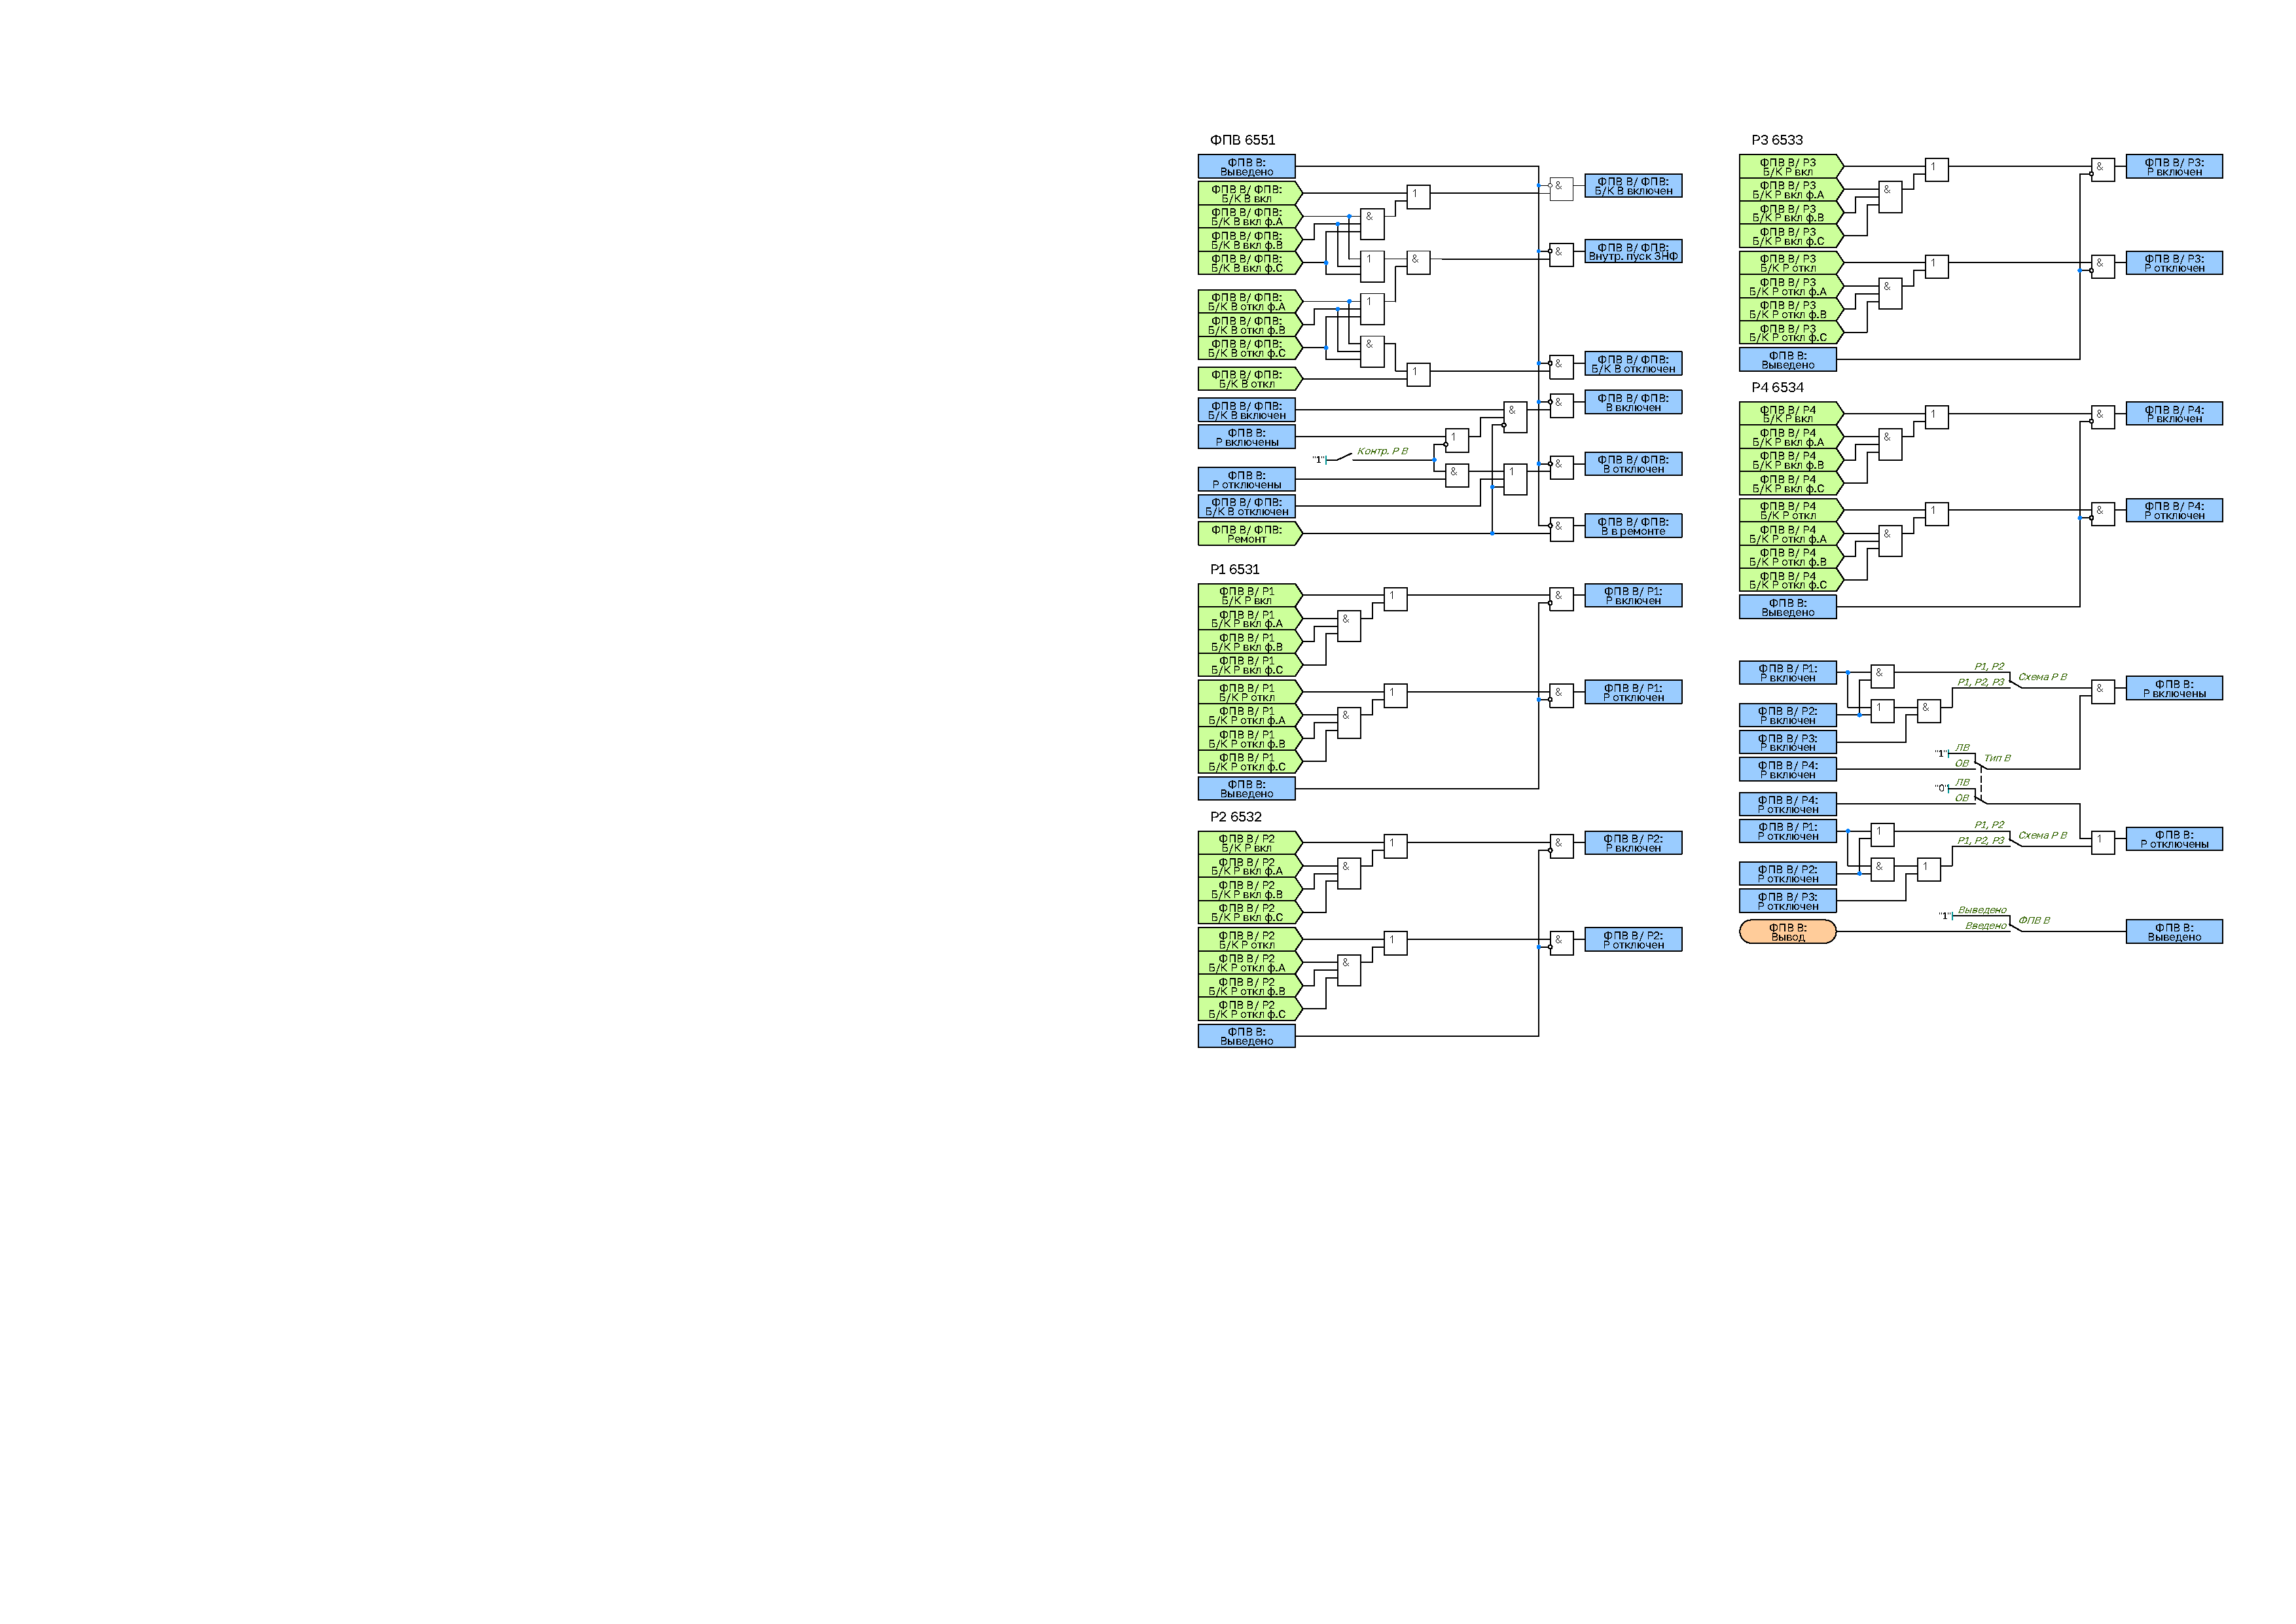
\includegraphics[width=1\textwidth,height=1\textheight,keepaspectratio]{img47.pdf}
\captionof{figure}{Функциональная схема логики ФПВ \Qtwo}\label{pict_fpv:fpv2}
\end{figure}

\end{enumerate}
\color{unidarkgreen}{\subsection{Контроль перевода на ОВ}}
\color{black}

\begin{enumerate}
\item
Функциональный блок контроля перевода на обходной выключатель предназначен для формирования сигнала фиксации перевода на ОВ, а также сигнала несоответствия фактического состояния первиичной схемы и оперативного переключателя фиксации перевода на ОВ.

\item
Сигнал фиксации перевода на ОВ формируется по состоянию разъединителя обходной системы шин выключателя (Р4) с контролем состояния оперативного переключателя перевода на ОВ.

\ifbool{isLV}{
\item
Функциональная схема логики контроля перевода на обходной выключатель приведена на рисунке \ref{pict_ksn:kpov}. Уставки КПОВ представлены в таблице \ref{app_set:kpov}.
}

\ifbool{isDZAT}{
\item
Функциональная схема логики контроля перевода на обходной выключатель приведена на рисунке \ref{pict_ksn:kpov}. Уставки КПОВ ВН представлены в таблице \ref{app_set:kpovvn}. Уставки КПОВ СН представлены в таблице \ref{app_set:kpovsn}.
}

\vspace{2mm}
\begin{figure}[H]
\centering
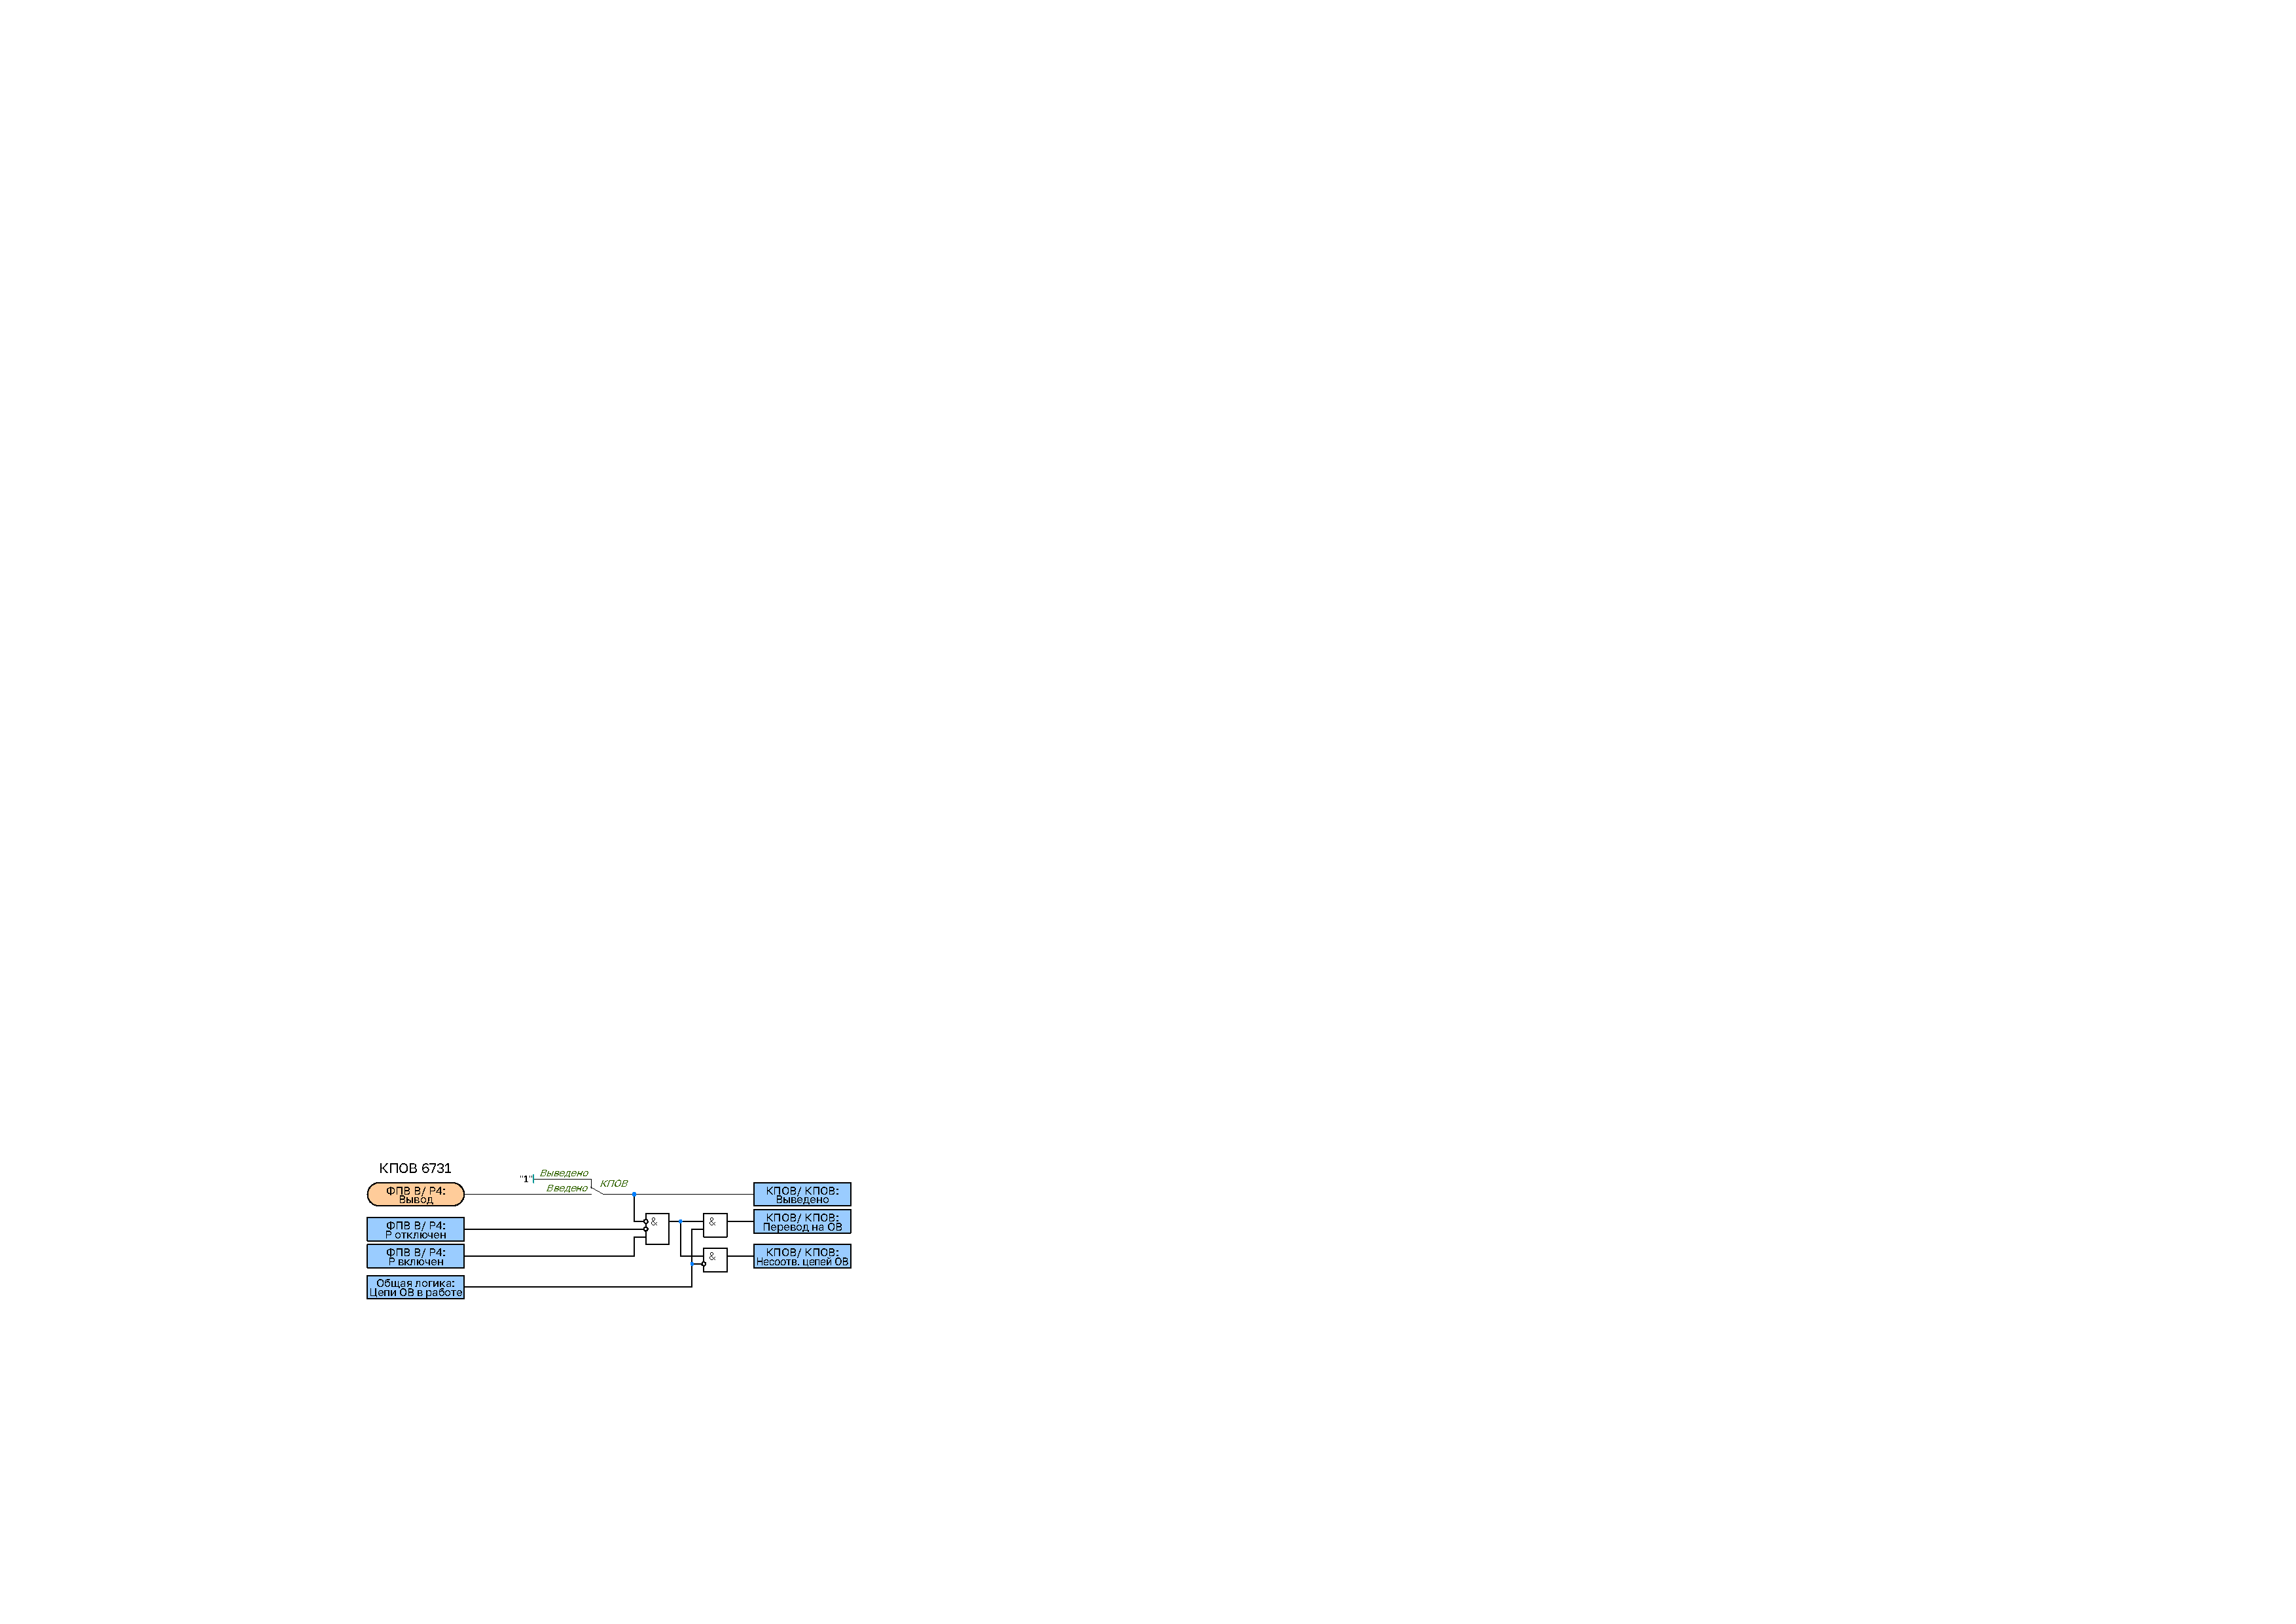
\includegraphics[width=0.8\textwidth,height=0.8\textheight,keepaspectratio]{img48.pdf}
\captionof{figure}{Функциональная схема логики контроля перевода на ОВ}\label{pict_ksn:kpov}
\end{figure}

\end{enumerate}\color{unidarkgreen}{\subsection{Cигнализация}}
\color{black}

\begin{enumerate}

\item
Устройство формирует выходное воздействие на сигнализацию «Срабатывание» по схеме «ИЛИ» в следующих случаях:
\begin{itemize}
\item Срабатывание ДЗТ;
\item Срабатывание газовых и технологических защит;
\item Срабатывание МТЗ НН;
\item Срабатывание ЗПО;
\item Срабатывание ЗП;
\item Срабатывание УРОВ;
\item Срабатывание внешних защит.
\end{itemize}

\item
Устройство формирует выходное воздействие на сигнализацию «Неисправность» по схеме «ИЛИ» в следующих случаях:
\begin{itemize}
\item Неисправность цепей тока ДЗТ;
\item Снижение изоляции цепей газовых и технологических защит;
\item Минимальный/максимальный уровень масла защищаемого оборудования;
\item Отказ/неисправность системы охлаждения АТ;
\item Неисправность цепей напряжения стороны НН;
\item Неисправность силового выключателя;
\item Снижение изоляции ошиновки НН;
\item Нарушение режима по испытательным блокам и/или переключателям в выходных цепях;
\item Потеря GOOSE-сообщения;
\item Срабатывание внешней функции на сигнализацию;
\item Неисправность цепей оперативного тока.
\end{itemize}

\begin{figure}[H]
\centering
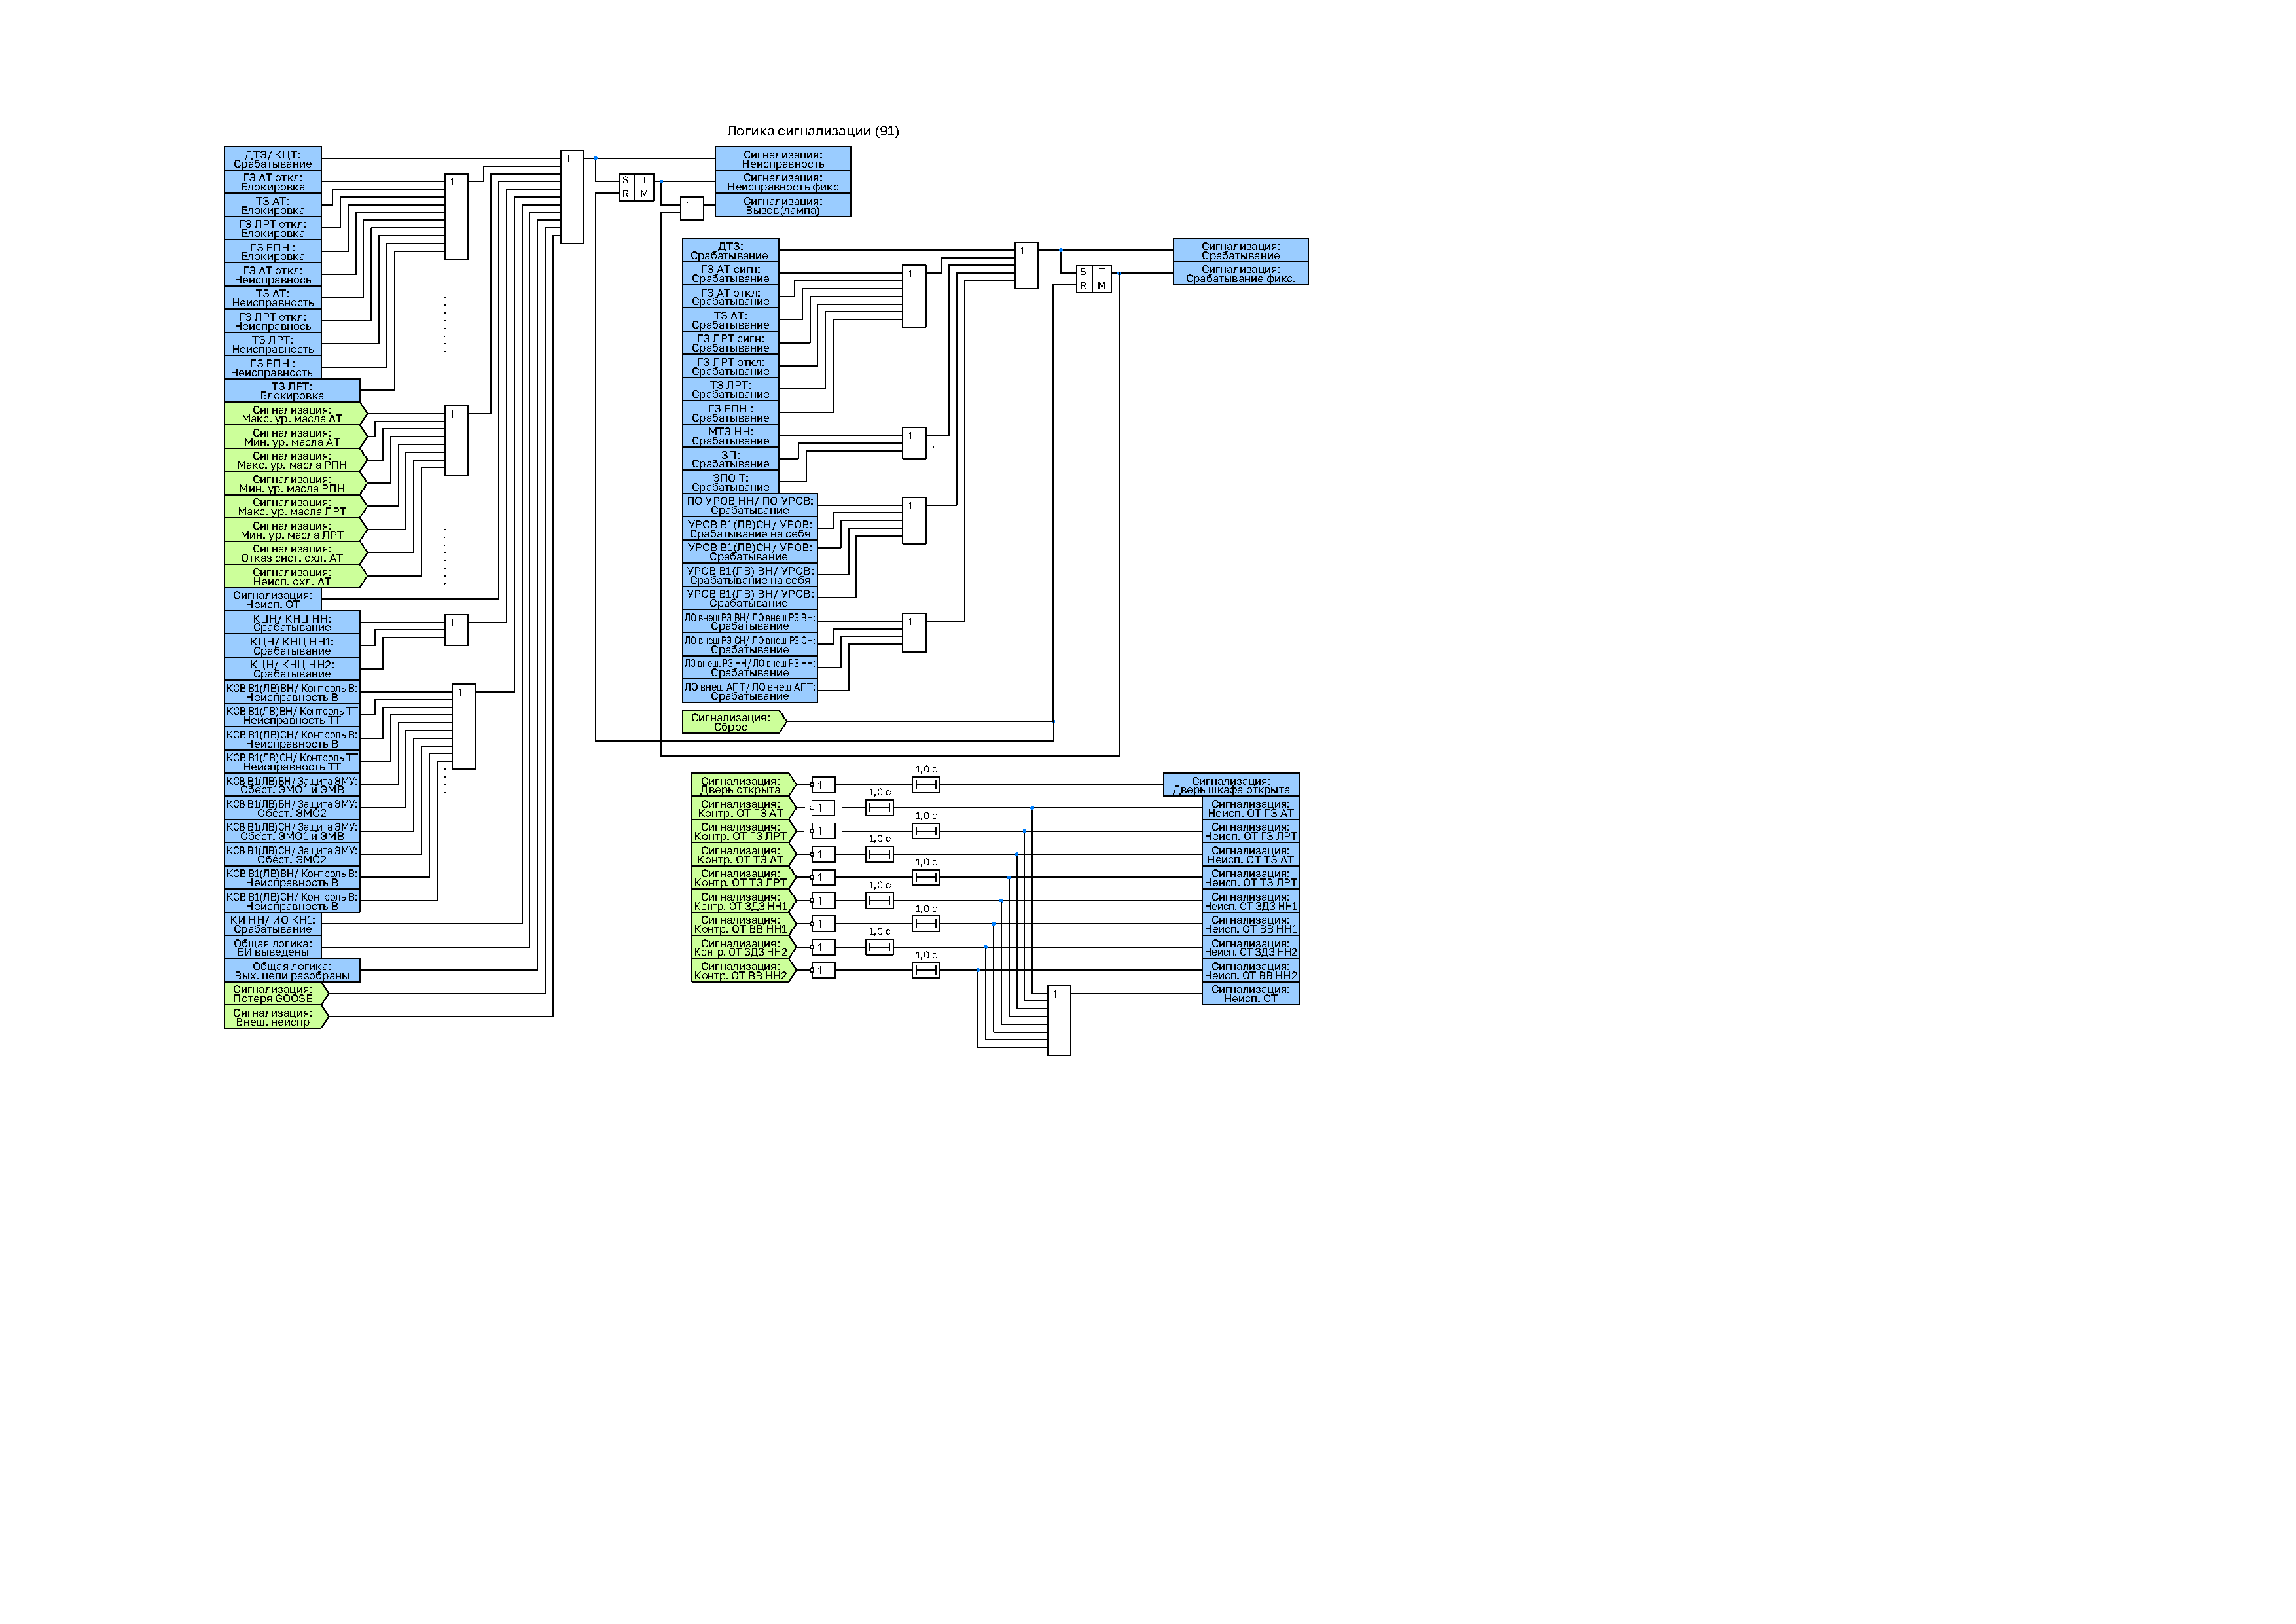
\includegraphics[width=1\textwidth,height=1\textheight,keepaspectratio]{img49.pdf}
\captionof{figure}{Функциональная схема логики блока сигнализации}\label{pic:SIGN}
\end{figure}

\end{enumerate}\color{unidarkgreen}{\subsection{Общая логика}}
\color{black}

\begin{enumerate}[label=\arabic{section}.\arabic{subsection}.\arabic*,  align=left, labelsep=4pt, leftmargin=0pt, itemindent=57pt]

\item
На рисунке \ref{pic:GL} представлена функциональная схема общей логики. Уставки общей логики представлены в таблице \ref{app_set:obshlog}. 

\begin{figure}[H]
\centering
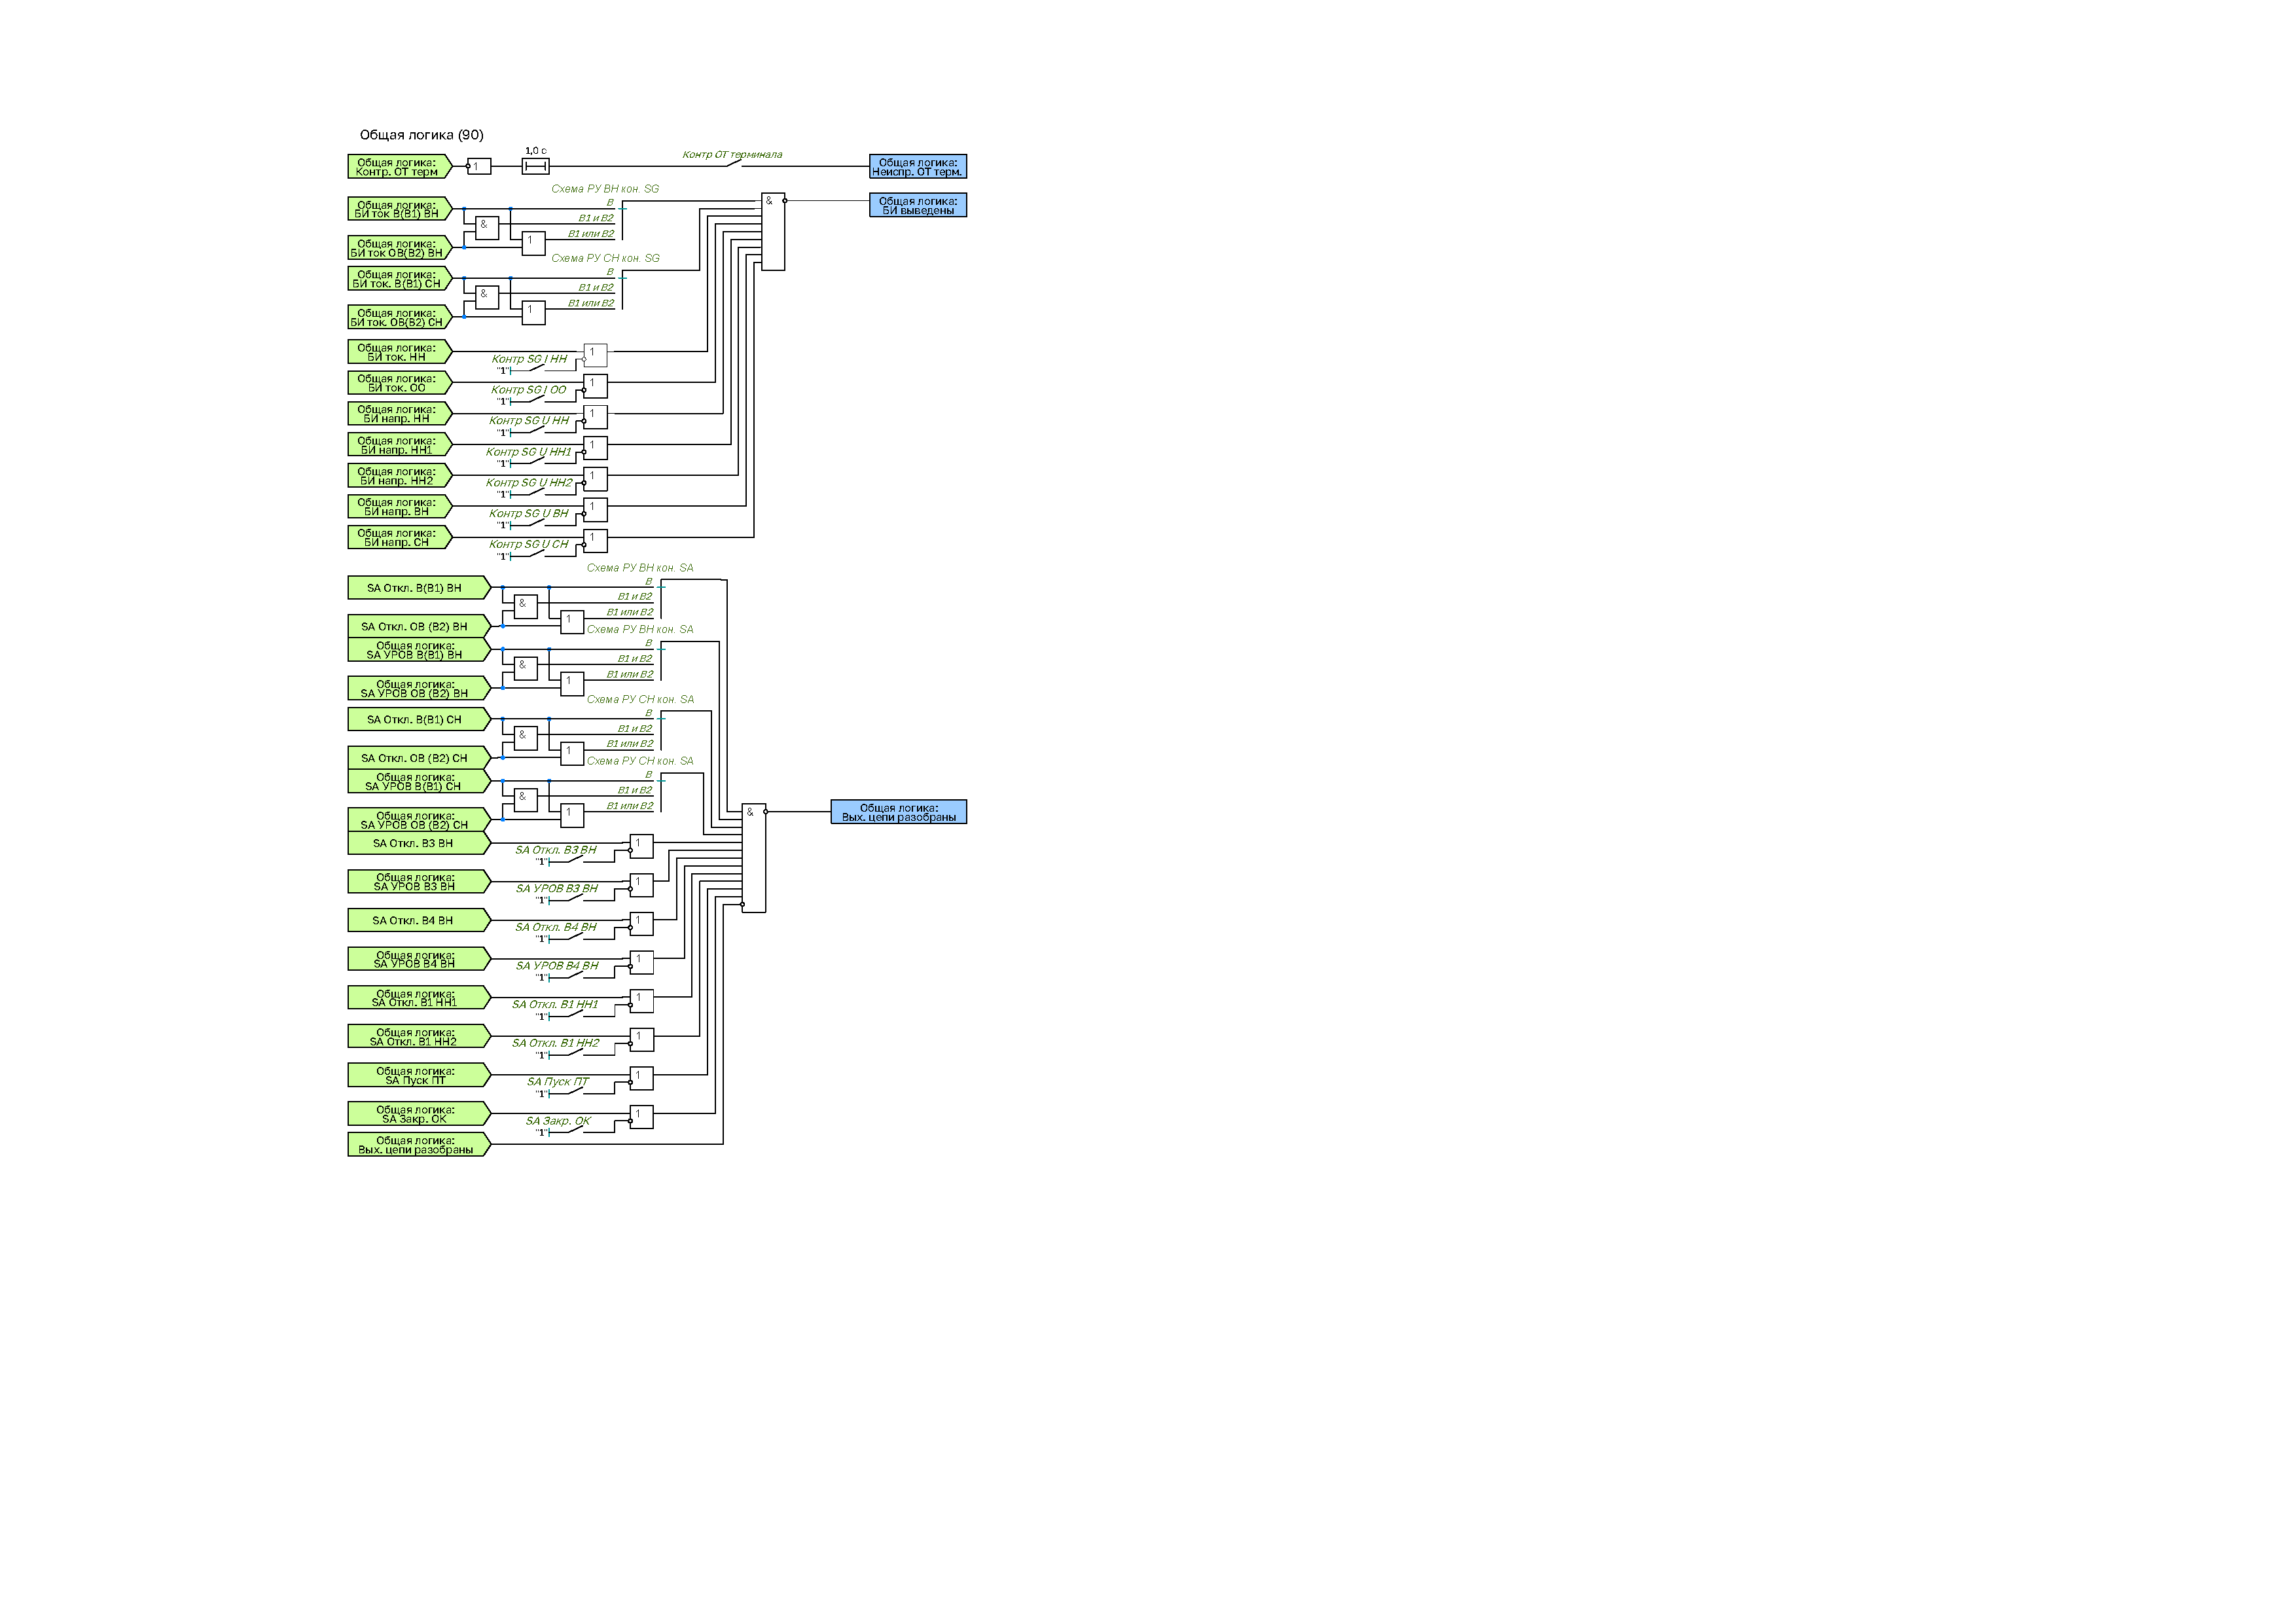
\includegraphics[width=0.9\textwidth,height=0.9\textheight,keepaspectratio]{img50.pdf}
\captionof{figure}{Функциональная схема общей логики}\label{pic:GL}
\end{figure}

\end{enumerate}\newpage
\color{unidarkgreen}\section[Использование по назначению]{Использование по назначению}\label{sec:using}
\color{black}

\color{unidarkgreen}\subsection{Эксплуатационные ограничения}\color{black}
Климатические условия эксплуатации должны соответствовать требованиям документа ЮТКБ.656122.609 РЭ «Устройство защиты и автоматики серии «ЮНИТ-М300». Руководство по эксплуатации общее».

\color{unidarkgreen}\subsection{Подготовка устройства к использованию}\color{black}
Меры безопасности при подготовке устройства, порядок проведения внешнего осмотра устройства перед использованием, требования к монтажу устройства, подключение к персональному компьютеру и устройству «ЮНИТ-ИЧМ» приводится в документации ЮТКБ.656122.609 РЭ «Устройство защиты и автоматики серии «ЮНИТ-М300». Руководство по эксплуатации общее».

\color{unidarkgreen}\subsection{Работа с устройством}\color{black}

\begin{enumerate}[label=\arabic{section}.\arabic{subsection}.\arabic*, labelsep=4pt, leftmargin=0pt, itemindent=57pt]
    \item
    Взаимодействие с устройством осуществляется при помощи подключаемого устройства «ЮНИТ-ИЧМ» или через персональный компьютер с установленным программным обеспечением «ЮНИТ-СЕРВИС». Руководство по устройству «ЮНИТ-ИЧМ» представлено в документе ЮТКБ.656132.701 РЭ «Блок интерфейсный «ЮНИТ-ИЧМ». Руководство по эксплуатации». Руководство по использованию программного обеспечения представлено в документе RU.37182817.00001.02.34.01 «Программное обеспечение мониторинга и параметрирования «ЮНИТ-СЕРВИС». Руководство пользователя».
    
    
    \end{enumerate}
    
    \par
    Описание работы с устройством (включение, способы управления устройством, обновление встроенного программного обеспечения, неисправности и методы их устранения) приводится в документации ЮТКБ.656122.609 РЭ «Устройство защиты и автоматики серии «ЮНИТ-М300». Руководство по эксплуатации общее».\newpage
\color{unidarkgreen}\section[Техническое обслуживание и ремонт]{Техническое обслуживание и ремонт}\label{sec:techrepair}
\color{black}

\color{unidarkgreen}\subsection{Техническое обслуживание устройства}\color{black}

\begin{enumerate}[label=\arabic{section}.\arabic{subsection}.\arabic*, labelsep=4pt, leftmargin=0pt, itemindent=57pt]

\item\sloppy
Процесс  технического  обслуживания  устройств  релейной  защиты  регламентирован  приказом Минэнерго  России  «Об  утверждении  Правил  технического  обслуживания  устройств  и  комплексов релейной  защиты  и  автоматики  и  внесении  изменений  в  требования  к  обеспечению  надежности электроэнергетических  систем,  надежности  и  безопасности  объектов  электроэнергетики  и энергопринимающих установок».
\item
Техническое обслуживание устройств «ЮНИТ-М300» должно выполняться в соответствии с документом ЮТКБ.656122.609 ИС – «Устройства защиты и автоматики серии «ЮНИТ-М300». Инструкция эксплуатационная специальная. Методические указания по выполнению технического обслуживания».

\end{enumerate}

\color{unidarkgreen}\subsection{Текущий ремонт}\color{black}

\begin{enumerate}[label=\arabic{section}.\arabic{subsection}.\arabic*, labelsep=4pt, leftmargin=0pt, itemindent=57pt]

\item
Устройство серии «ЮНИТ-М300», как было описано выше, выполнено с использованием микропроцессорных технологий, поэтому необходимость в его текущем ремонте отсутствует. Работоспособность и безотказность работы устройства обеспечивается функционированием системы самодиагностики.
\item
Углубленная самодиагностика аппаратных средств, а также состояние программной памяти, памяти данных  и  буферной  памяти  производится  при  включении  устройства.  Поэтому  при  возникновении сообщений о критических или некритических ошибках от системы самодиагностики, даже при возможности устранения  их  своими  силами,  следует  обратиться  на  предприятие-изготовитель для  консультации или проведения регламентных работ.
\item 
Поводом  для  обращения  на  предприятие-изготовитель  являются  также  признаки  нехарактерного нагрева или перегрева отдельных элементов, участков или частей устройства.
\item
Вышедшие  из  строя  устройства  должны  проходить  ремонт  на  предприятии-изготовителе, обеспечивающем  гарантийное  и  послегарантийное  обслуживание, адрес которого  указан  в  паспорте устройства.  В  качестве  ЗИП,  если  это  предусмотрено  договором  поставки,  могут  предоставляться устройства  «ЮНИТ-М300» с необходимыми  конфигурациями,  позволяющие  оперативно  произвести  замену вышедших из строя устройств.
\item
Перечень сигналов самодиагностики приведен в документации ЮТКБ.656122.609 РЭ «Устройство защиты и автоматики серии «ЮНИТ-М300». Руководство по эксплуатации общее».
\end{enumerate}


\vspace{5mm}
\color{unidarkgreen}\section[Транспортирование, хранение и консервация]{Транспортирование, хранение и консервация}\label{sec:trans}
\color{black}


Более подробно об условиях транспортирования и хранения устройства можно узнать в соответствующем разделе документации ЮТКБ.656122.609 РЭ «Устройство защиты и автоматики серии «ЮНИТ-М300». Руководство по эксплуатации общее». 

\vspace{3mm}
\color{unidarkgreen}\section[Утилизация]{Утилизация}\label{sec:util}
\color{black}

\begin{enumerate}[label=\arabic{section}.\arabic*, labelsep=4pt, leftmargin=0pt, itemindent=57pt]

\item
Демонтаж и утилизация устройства не требуют применения специальных мер безопасности и выполняются без применения специальных приспособлений и инструментов.
\item
Более подробно о способах утилизации устройства можно узнать в соответствующем разделе документации ЮТКБ.656122.609 РЭ «Устройство защиты и автоматики серии «ЮНИТ-М300». Руководство по эксплуатации общее».

\end{enumerate}

\vspace{3mm}
\color{unidarkgreen}\section[Гарантия изготовителя]{Гарантия изготовителя}\label{sec:garantee}
\color{black}

\begin{enumerate}[label=\arabic{section}.\arabic*, labelsep=4pt, leftmargin=0pt, itemindent=57pt]

\item
Гарантийный срок эксплуатации устройства составляет 36 месяцев со дня ввода устройства в эксплуатацию, но не более 40 месяцев с даты производства предприятием-изготовителем или с момента проследования через государственную границу при поставках на экспорт.
\item
Более подробно о гарантийных обязательствах изготовителя устройства можно узнать в соответствующем разделе документации ЮТКБ.656122.609 РЭ «Устройство защиты и автоматики серии «ЮНИТ-М300». Руководство по эксплуатации общее». 

\end{enumerate}\vspace{3mm}
\color{unidarkgreen}\section[Техническая поддержка]{Техническая поддержка}\label{sec:support}
\color{black}

\noindent
Сервисный  центр  ООО  «Юнител  Инжиниринг»  принимает  заявки  от  потребителей  о  качестве функционирования  оборудования  и  ПО,  оказывает  консультационные  услуги  при  поиске  и  устранении неисправностей.
\par
\noindent
Заявки от потребителей принимаются  по  телефонной  связи  (тел.:  +7 (495) 165-99-98) и (или) по электронной почте:
\vskip 1mm

\href{mailto:rza@uni-eng.ru}{\color{unigreen}\uline{rza@uni-eng.ru}}
\vskip 1mm

\href{mailto:info@uni-eng.ru}{\color{unigreen}\uline{info@uni-eng.ru}}
\vskip 1mm

\noindent
Форму заявки можно скачать по ссылке: 

\href{https://uni-eng.ru/support/servisnyy-tsentr/}{\color{unigreen}\uline{https://uni-eng.ru/support/servisnyy-tsentr/}}.



\appendixtitleon
\appendixtitletocon

\settocdepth{section}

\makeatletter
\renewcommand{\Asbuk}[1]{\expandafter\@Asbuk\csname c@#1\endcsname}
\def\@Asbuk#1{\ifcase#1\or
 А\or Б\or В\or Г\or Д\or Е\or Ж\or И\or К\or Л\or М\or Н\or О\or П\or Р\or С\or Т\or У\or Ф\or Х\or Ц\or Ч\or Ш\or Щ\or Э\or Ю\or Я\else\@ctrerr\fi}
\makeatother

\begin{appendices}

\renewcommand{\thesection}{\Asbuk{section}}

\titleformat{\section}[display]
  {\normalfont\large\bfseries}
  {\centering Приложение\ \thesection}
  {0pt}{\large\centering}




\newpage
\newcommand{\startTable}[2]{%
    \footnotesize
    \begin{longtable}{|>{\centering\arraybackslash}m{3.8cm}|>{\centering\arraybackslash}m{3.3cm}|>{\centering\arraybackslash}m{2.7cm}|>{\centering\arraybackslash}m{2.8cm}|>{\centering\arraybackslash}m{3.0cm}|}
    \caption{#1\hfill\vspace{-0.5\baselineskip}}\label{#2}\\
    \hline
    \rowcolor{gray!20}
    Наименование уставки & Значение/Диапазон & Единица измерения & Шаг & Значение по умолчанию \\
    \hline
    \endfirsthead
    \caption*{\hspace{3pt}\emph{Продолжение таблицы \ref{#2}\hfill\vspace{-0.5\baselineskip}}} \\
    \hline
    \rowcolor{gray!20}
    Наименование уставки & Значение/Диапазон & Единица измерения & Шаг & Значение по умолчанию \\
    \hline
    \endhead
}

\newcommand{\stopTable}{%
    \end{longtable}%
    \normalsize
}
\color{unidarkgreen}{\section[(обязательное) Уставки функций РЗА]{(обязательное)\\Уставки функций РЗА}\label{app:set}}
\color{black}

\setlength{\extrarowheight}{0.06cm}



\par
Уставки ДТЗ представлены в таблице \ref{app_set:dzt}.

\startTable{Параметры для настройки ДТЗ}{app_set:dzt}

\multicolumn{5}{|c|}{ ДТЗ } \\ \hline 
\centering ДТЗ фВ & \centering Выведено \\ Введено & \centering --- & \centering --- & \centering \arraybackslash Выведено \\
\hline
\centering Iср диф & \centering 0,100 ... 2,000 & \centering о.е. & \centering 0,001 & \centering \arraybackslash 0,200 \\
\hline
\centering Кв(Iср диф) & \centering 0,00 ... 1,00 & \centering о.е. & \centering 0,01 & \centering \arraybackslash 0,80 \\
\hline
\multicolumn{5}{|c|}{ КЦТ } \\ \hline 
\centering Iнеиспр ДТЗ & \centering 0,04 ... 30,00 & \centering о.е. & \centering 0,01 & \centering \arraybackslash 0,10 \\
\hline
\centering Кв (Iнеиспр) & \centering 0,00 ... 1,00 & \centering  & \centering 0,01 & \centering \arraybackslash 0,95 \\
\hline
\centering Тнеиспр ДТЗ & \centering 0 ... 300000 & \centering мс & \centering 5 & \centering \arraybackslash 10000 \\
\hline
\centering Контр изм цеп ДТЗ & \centering Введено \\ Выведено & \centering --- & \centering --- & \centering \arraybackslash Введено \\
\hline
\centering фВ & \centering Введено \\ Выведено & \centering --- & \centering --- & \centering \arraybackslash Введено \\
\hline
\multicolumn{5}{|c|}{ ДТЗт } \\ \hline 
\centering Iср диф & \centering 0,100 ... 2,000 & \centering о.е. & \centering 0,001 & \centering \arraybackslash 0,200 \\
\hline
\centering Iт1 & \centering 0,200 ... 1,500 & \centering о.е. & \centering 0,001 & \centering \arraybackslash 1,000 \\
\hline
\centering Кт1 & \centering 0,100 ... 1,000 & \centering о.е. & \centering 0,001 & \centering \arraybackslash 0,500 \\
\hline
\centering Iт2 & \centering 1,000 ... 3,000 & \centering о.е. & \centering 0,001 & \centering \arraybackslash 2,000 \\
\hline
\centering Кт2 & \centering 0,200 ... 1,000 & \centering о.е. & \centering 0,001 & \centering \arraybackslash 0,750 \\
\hline
\centering Кв (Iср диф) & \centering 0,00 ... 1,00 & \centering  & \centering 0,01 & \centering \arraybackslash 0,80 \\
\hline
\centering фВ & \centering Введено \\ Выведено & \centering --- & \centering --- & \centering \arraybackslash Введено \\
\hline
\centering ДТЗт & \centering Введено \\ Выведено & \centering --- & \centering --- & \centering \arraybackslash Введено \\
\hline
\multicolumn{5}{|c|}{ ДТО } \\ \hline 
\centering Iср ДТО & \centering 1,000 ... 20,000 & \centering о.е. & \centering 0,001 & \centering \arraybackslash 20,000 \\
\hline
\centering Кв (Iср) & \centering 0,00 ... 1,00 & \centering  & \centering 0,01 & \centering \arraybackslash 0,95 \\
\hline
\centering фВ & \centering Введено \\ Выведено & \centering --- & \centering --- & \centering \arraybackslash Введено \\
\hline
\centering ДТО & \centering Введено \\ Выведено & \centering --- & \centering --- & \centering \arraybackslash Введено \\
\hline
\multicolumn{5}{|c|}{ Д2г } \\ \hline 
\centering I2г/I1г ДТЗт & \centering 0,050 ... 1,000 & \centering о.е. & \centering 0,001 & \centering \arraybackslash 0,500 \\
\hline
\centering Кв (I2(5)г/I1г) & \centering 0,00 ... 1,00 & \centering  & \centering 0,01 & \centering \arraybackslash 0,95 \\
\hline
\centering Iср диф & \centering 0,000 ... 2,000 & \centering о.е. & \centering 0,001 & \centering \arraybackslash 0,200 \\
\hline
\centering Кв (Iср диф) & \centering 0,00 ... 1,00 & \centering  & \centering 0,01 & \centering \arraybackslash 0,95 \\
\hline
\centering 0.01 с & \centering 0 ... 10 & \centering мc & \centering 5 & \centering \arraybackslash 10 \\
\hline
\centering 0.02 с & \centering 0 ... 20 & \centering мc & \centering 5 & \centering \arraybackslash 20 \\
\hline
\centering фВ & \centering Введено \\ Выведено & \centering --- & \centering --- & \centering \arraybackslash Введено \\
\hline
\centering Перекр блок 2г & \centering Откл \\ 1 из 3 \\ 2 из 3 & \centering --- & \centering --- & \centering \arraybackslash Откл \\
\hline
\centering Тперекр блок 2г & \centering 100 ... 1000 & \centering мc & \centering 5 & \centering \arraybackslash 100 \\
\hline
\centering Блок 2г ДТЗт & \centering Введено \\ Выведено & \centering --- & \centering --- & \centering \arraybackslash Введено \\
\hline
\multicolumn{5}{|c|}{ Д5г } \\ \hline 
\centering I5г/I1г ДТЗт & \centering 0,050 ... 1,000 & \centering о.е. & \centering 0,001 & \centering \arraybackslash 0,500 \\
\hline
\centering Кв (I2(5)г/I1г) & \centering 0,00 ... 1,00 & \centering  & \centering 0,01 & \centering \arraybackslash 0,95 \\
\hline
\centering Iср диф & \centering 0,000 ... 2,000 & \centering о.е. & \centering 0,001 & \centering \arraybackslash 0,200 \\
\hline
\centering Кв (Iср диф) & \centering 0,00 ... 1,00 & \centering  & \centering 0,01 & \centering \arraybackslash 0,95 \\
\hline
\centering 0.01 с & \centering 0 ... 10 & \centering мc & \centering 5 & \centering \arraybackslash 10 \\
\hline
\centering 0.02 с & \centering 0 ... 20 & \centering мc & \centering 5 & \centering \arraybackslash 20 \\
\hline
\centering фВ & \centering Введено \\ Выведено & \centering --- & \centering --- & \centering \arraybackslash Введено \\
\hline
\centering Перекр блок 5г & \centering Откл \\ 1 из 3 \\ 2 из 3 & \centering --- & \centering --- & \centering \arraybackslash Откл \\
\hline
\centering Тперекр блок 5г & \centering 100 ... 1000 & \centering мc & \centering 5 & \centering \arraybackslash 100 \\
\hline
\centering Блок 5г ДТЗт & \centering Введено \\ Выведено & \centering --- & \centering --- & \centering \arraybackslash Введено \\
\hline
\stopTable



\par
Уставки МТЗ НН представлены в таблице \ref{app_set:mtz}.

\startTable{Параметры для настройки МТЗ НН}{app_set:mtz}

\multicolumn{5}{|c|}{ МТЗ-1 } \\ \hline 
\centering Iср МТЗ-1 НН & \centering 0,04 ... 30,00 & \centering о.е. & \centering 0,01 & \centering \arraybackslash 30,00 \\
\hline
\centering Тср МТЗ-1 НН & \centering 0 ... 300000 & \centering мс & \centering 5 & \centering \arraybackslash 300000 \\
\hline
\centering МТЗ-1 НН & \centering Введено \\ Выведено & \centering --- & \centering --- & \centering \arraybackslash Введено \\
\hline
\centering Режим КПОН МТЗ-1 НН & \centering Введено \\ Выведено & \centering --- & \centering --- & \centering \arraybackslash Введено \\
\hline
\centering Режим БНТ МТЗ-1 НН & \centering Введено \\ Выведено & \centering --- & \centering --- & \centering \arraybackslash Введено \\
\hline
\multicolumn{5}{|c|}{ МТЗ-2 } \\ \hline 
\centering Iср МТЗ-2 НН & \centering 0,04 ... 30,00 & \centering о.е. & \centering 0,01 & \centering \arraybackslash 30,00 \\
\hline
\centering Тср МТЗ-2 НН & \centering 0 ... 300000 & \centering мс & \centering 5 & \centering \arraybackslash 300000 \\
\hline
\centering МТЗ-2 НН & \centering Введено \\ Выведено & \centering --- & \centering --- & \centering \arraybackslash Введено \\
\hline
\centering Режим КПОН МТЗ-2 НН & \centering Введено \\ Выведено & \centering --- & \centering --- & \centering \arraybackslash Введено \\
\hline
\centering Режим БНТ МТЗ-2 НН & \centering Введено \\ Выведено & \centering --- & \centering --- & \centering \arraybackslash Введено \\
\hline
\multicolumn{5}{|c|}{ ТО } \\ \hline 
\centering Iср ТО НН & \centering 0,04 ... 30,00 & \centering о.е. & \centering 0,01 & \centering \arraybackslash 30,00 \\
\hline
\centering Тср ТО НН & \centering 0 ... 300000 & \centering мс & \centering 5 & \centering \arraybackslash 300000 \\
\hline
\centering  ТО НН & \centering Введено \\ Выведено & \centering --- & \centering --- & \centering \arraybackslash Введено \\
\hline
\centering Режим БНТ ТО НН & \centering Введено \\ Выведено & \centering --- & \centering --- & \centering \arraybackslash Введено \\
\hline
\multicolumn{5}{|c|}{ БНТ } \\ \hline 
\centering I2г/I1г МТЗ НН & \centering 0,00 ... 1,00 & \centering о.е. & \centering 0,01 & \centering \arraybackslash 0,20 \\
\hline
\centering kв=0.95 & \centering 0,00 ... 1,00 & \centering  & \centering 0,01 & \centering \arraybackslash 0,95 \\
\hline
\centering 0.04Iном (Iразр БНТ МТЗ НН) & \centering 0,04 ... 30,00 & \centering о.е & \centering 0,01 & \centering \arraybackslash 0,04 \\
\hline
\centering kв=1 & \centering 0,00 ... 1,00 & \centering  & \centering 0,01 & \centering \arraybackslash 1,00 \\
\hline
\centering БНТ МТЗ НН & \centering Введено \\ Выведено & \centering --- & \centering --- & \centering \arraybackslash Введено \\
\hline
\centering Iблок БНТ МТЗ НН & \centering 0,04 ... 30,00 & \centering о.е. & \centering 0,01 & \centering \arraybackslash 30,00 \\
\hline
\end{longtable}
\normalsize



\par
Уставки КПОН представлены в таблице \ref{app_set:kpon}.

\startTable{Параметры для настройки КПОН}{app_set:kpon}

\multicolumn{5}{|c|}{ КПОН НН1 } \\ \hline 
\centering U2 КПОН НН1 & \centering 0,0050 ... 1,5000 & \centering о.е & \centering 0,0001 & \centering \arraybackslash 1,5000 \\
\hline
\centering Uл КПОН НН1 & \centering 0,0050 ... 1,5000 & \centering о.е & \centering 0,0001 & \centering \arraybackslash 0,0050 \\
\hline
\centering Тип КПОН НН1 & \centering Umin, U2 \\ Umin \\ Внеш & \centering --- & \centering --- & \centering \arraybackslash Umin, U2 \\
\hline
\centering  КПОН НН1 & \centering Введено \\ Выведено & \centering --- & \centering --- & \centering \arraybackslash Введено \\
\hline
\centering Неиспр ТН КПОН НН1 & \centering Выведено \\ Пуск КПОН \\ Блок КПОН & \centering --- & \centering --- & \centering \arraybackslash Выведено \\
\hline
\multicolumn{5}{|c|}{ КПОН НН2 } \\ \hline 
\centering U2 КПОН НН2 & \centering 0,0050 ... 1,5000 & \centering о.е & \centering 0,0001 & \centering \arraybackslash 1,5000 \\
\hline
\centering Uл КПОН НН2 & \centering 0,0050 ... 1,5000 & \centering о.е & \centering 0,0001 & \centering \arraybackslash 0,0050 \\
\hline
\centering Тип КПОН НН2 & \centering Umin, U2 \\ Umin \\ Внеш & \centering --- & \centering --- & \centering \arraybackslash Umin, U2 \\
\hline
\centering  КПОН НН2 & \centering Введено \\ Выведено & \centering --- & \centering --- & \centering \arraybackslash Введено \\
\hline
\centering Неиспр ТН КПОН НН2 & \centering Выведено \\ Пуск КПОН \\ Блок КПОН & \centering --- & \centering --- & \centering \arraybackslash Выведено \\
\hline
\multicolumn{5}{|c|}{ КПОН НН } \\ \hline 
\centering U2 КПОН НН & \centering 0,0050 ... 1,5000 & \centering о.е & \centering 0,0001 & \centering \arraybackslash 1,5000 \\
\hline
\centering Uл КПОН НН & \centering 0,0050 ... 1,5000 & \centering о.е & \centering 0,0001 & \centering \arraybackslash 0,0050 \\
\hline
\centering Тип КПОН НН & \centering Umin, U2 \\ Umin \\ Внеш & \centering --- & \centering --- & \centering \arraybackslash Umin, U2 \\
\hline
\centering КПОН НН & \centering Введено \\ Выведено & \centering --- & \centering --- & \centering \arraybackslash Введено \\
\hline
\centering Неиспр ТН КПОН НН & \centering Выведено \\ Пуск КПОН \\ Блок КПОН & \centering --- & \centering --- & \centering \arraybackslash Выведено \\
\hline
\end{longtable}
\normalsize




\par
Уставки отключающей ступени ГЗ АТ представлены в таблице \ref{app_set:gzotkl}.

\startTable{Параметры для настройки отключающей ступени ГЗ АТ}{app_set:gzotkl}

\multicolumn{5}{|c|}{ ГЗ АТ откл } \\ \hline 
\centering ГЗ АТ откл 1 цепь & \centering Введено \\ Выведено & \centering --- & \centering --- & \centering \arraybackslash Введено \\
\hline
\centering ГЗ АТ откл 2 цепь & \centering Введено \\ Выведено & \centering --- & \centering --- & \centering \arraybackslash Введено \\
\hline
\centering Блокировка ГЗ АТ откл & \centering Введено \\ Выведено & \centering --- & \centering --- & \centering \arraybackslash Введено \\
\hline
\centering Тбл ГЗ АТ откл & \centering 0 ... 300000 & \centering мс & \centering 5 & \centering \arraybackslash 300000 \\
\hline
\multicolumn{5}{|c|}{ ГЗ откл 1 цепь } \\ \hline 
\centering Блокировка & \centering Введено \\ Выведено & \centering --- & \centering --- & \centering \arraybackslash Введено \\
\hline
\centering ГЗ (ТЗ) откл & \centering Введено \\ Выведено & \centering --- & \centering --- & \centering \arraybackslash Введено \\
\hline
\centering Тбл & \centering 0 ... 300000 & \centering мс & \centering 5 & \centering \arraybackslash 300000 \\
\hline
\multicolumn{5}{|c|}{ ГЗ откл 2 цепь } \\ \hline 
\centering Блокировка & \centering Введено \\ Выведено & \centering --- & \centering --- & \centering \arraybackslash Введено \\
\hline
\centering ГЗ (ТЗ) откл & \centering Введено \\ Выведено & \centering --- & \centering --- & \centering \arraybackslash Введено \\
\hline
\centering Тбл & \centering 0 ... 300000 & \centering мс & \centering 5 & \centering \arraybackslash 300000 \\
\hline
\end{longtable}
\normalsize



\par
Уставки сигнальной ступени ГЗ АТ представлены в таблице \ref{app_set:gzsign}.

\startTable{Параметры для настройки сигнальной ступени ГЗ АТ}{app_set:gzsign}

\multicolumn{5}{|c|}{ ГЗ АТ сигн } \\ \hline 
\centering ГЗ АТ сигн 1 цепь & \centering Введено \\ Выведено & \centering --- & \centering --- & \centering \arraybackslash Введено \\
\hline
\centering ГЗ АТ сигн 2 цепь & \centering Введено \\ Выведено & \centering --- & \centering --- & \centering \arraybackslash Введено \\
\hline
\centering Откл от ГЗ АТ сигн & \centering Введено \\ Выведено & \centering --- & \centering --- & \centering \arraybackslash Введено \\
\hline
\multicolumn{5}{|c|}{ ГЗ сигн 2 цепь } \\ \hline 
\centering ГЗ (ТЗ) сигн & \centering Введено \\ Выведено & \centering --- & \centering --- & \centering \arraybackslash Введено \\
\hline
\multicolumn{5}{|c|}{ ГЗ сигн 1 цепь } \\ \hline 
\centering ГЗ (ТЗ) сигн & \centering Введено \\ Выведено & \centering --- & \centering --- & \centering \arraybackslash Введено \\
\hline
\end{longtable}
\normalsize



\par
Уставки отключающей ступени ГЗ ЛРТ представлены в таблице \ref{app_set:gzlrtotkl}.

\startTable{Параметры для настройки отключающей ступени ГЗ ЛРТ}{app_set:gzlrtotkl}

\multicolumn{5}{|c|}{ ГЗ ЛРТ откл } \\ \hline 
\centering ГЗ ЛРТ откл 1 цепь & \centering Введено \\ Выведено & \centering --- & \centering --- & \centering \arraybackslash Введено \\
\hline
\centering ГЗ ЛРТ откл 2 цепь & \centering Введено \\ Выведено & \centering --- & \centering --- & \centering \arraybackslash Введено \\
\hline
\centering Блокировка ГЗ ЛРТ & \centering Введено \\ Выведено & \centering --- & \centering --- & \centering \arraybackslash Введено \\
\hline
\centering Тбл ГЗ ЛРТ & \centering 0 ... 300000 & \centering мс & \centering 5 & \centering \arraybackslash 300000 \\
\hline
\multicolumn{5}{|c|}{ ГЗ откл 1 цепь } \\ \hline 
\centering Блокировка & \centering Введено \\ Выведено & \centering --- & \centering --- & \centering \arraybackslash Введено \\
\hline
\centering ГЗ (ТЗ) откл & \centering Введено \\ Выведено & \centering --- & \centering --- & \centering \arraybackslash Введено \\
\hline
\centering Тбл & \centering 0 ... 300000 & \centering мс & \centering 5 & \centering \arraybackslash 300000 \\
\hline
\multicolumn{5}{|c|}{ ГЗ откл 2 цепь } \\ \hline 
\centering Блокировка & \centering Введено \\ Выведено & \centering --- & \centering --- & \centering \arraybackslash Введено \\
\hline
\centering ГЗ (ТЗ) откл & \centering Введено \\ Выведено & \centering --- & \centering --- & \centering \arraybackslash Введено \\
\hline
\centering Тбл & \centering 0 ... 300000 & \centering мс & \centering 5 & \centering \arraybackslash 300000 \\
\hline
\end{longtable}
\normalsize



\par
Уставки сигнальной ступени ГЗ ЛРТ представлены в таблице \ref{app_set:gzlrtsign}.

\startTable{Параметры для настройки сигнальной ступени ГЗ ЛРТ}{app_set:gzlrtsign}

\multicolumn{5}{|c|}{ ГЗ ЛРТ сигн } \\ \hline 
\centering ГЗ ЛРТ сигн 1 цепь & \centering Введено \\ Выведено & \centering --- & \centering --- & \centering \arraybackslash Введено \\
\hline
\centering ГЗ ЛРТ сигн 2 цепь & \centering Введено \\ Выведено & \centering --- & \centering --- & \centering \arraybackslash Введено \\
\hline
\centering Откл от ГЗ ЛРТ сигн & \centering Введено \\ Выведено & \centering --- & \centering --- & \centering \arraybackslash Введено \\
\hline
\multicolumn{5}{|c|}{ ГЗ сигн 2 цепь } \\ \hline 
\centering ГЗ (ТЗ) сигн & \centering Введено \\ Выведено & \centering --- & \centering --- & \centering \arraybackslash Введено \\
\hline
\multicolumn{5}{|c|}{ ГЗ сигн 1 цепь } \\ \hline 
\centering ГЗ (ТЗ) сигн & \centering Введено \\ Выведено & \centering --- & \centering --- & \centering \arraybackslash Введено \\
\hline
\end{longtable}
\normalsize



\par
Уставки ГЗ РПН представлены в таблице \ref{app_set:gzrpn}.

\startTable{Параметры для настройки ГЗ РПН}{app_set:gzrpn}

\multicolumn{5}{|c|}{ ГЗ РПН } \\ \hline 
\centering ГЗ РПН 1 цепь & \centering Введено \\ Выведено & \centering --- & \centering --- & \centering \arraybackslash Введено \\
\hline
\centering ГЗ РПН 2 цепь & \centering Введено \\ Выведено & \centering --- & \centering --- & \centering \arraybackslash Введено \\
\hline
\centering Блок ГЗ РПН & \centering Введено \\ Выведено & \centering --- & \centering --- & \centering \arraybackslash Введено \\
\hline
\centering Тбл ГЗ РПН & \centering 0 ... 300000 & \centering мс & \centering 5 & \centering \arraybackslash 300000 \\
\hline
\multicolumn{5}{|c|}{ ГЗ откл.фА 1 цепь } \\ \hline 
\centering Блокировка & \centering Введено \\ Выведено & \centering --- & \centering --- & \centering \arraybackslash Введено \\
\hline
\centering ГЗ (ТЗ) откл & \centering Введено \\ Выведено & \centering --- & \centering --- & \centering \arraybackslash Введено \\
\hline
\centering Тбл & \centering 0 ... 300000 & \centering мс & \centering 5 & \centering \arraybackslash 300000 \\
\hline
\multicolumn{5}{|c|}{ ГЗ откл.фА 2 цепь } \\ \hline 
\centering Блокировка & \centering Введено \\ Выведено & \centering --- & \centering --- & \centering \arraybackslash Введено \\
\hline
\centering ГЗ (ТЗ) откл & \centering Введено \\ Выведено & \centering --- & \centering --- & \centering \arraybackslash Введено \\
\hline
\centering Тбл & \centering 0 ... 300000 & \centering мс & \centering 5 & \centering \arraybackslash 300000 \\
\hline
\multicolumn{5}{|c|}{ ГЗ откл.фВ 1 цепь } \\ \hline 
\centering Блокировка & \centering Введено \\ Выведено & \centering --- & \centering --- & \centering \arraybackslash Введено \\
\hline
\centering ГЗ (ТЗ) откл & \centering Введено \\ Выведено & \centering --- & \centering --- & \centering \arraybackslash Введено \\
\hline
\centering Тбл & \centering 0 ... 300000 & \centering мс & \centering 5 & \centering \arraybackslash 300000 \\
\hline
\multicolumn{5}{|c|}{ ГЗ откл.фВ 2 цепь } \\ \hline 
\centering Блокировка & \centering Введено \\ Выведено & \centering --- & \centering --- & \centering \arraybackslash Введено \\
\hline
\centering ГЗ (ТЗ) откл & \centering Введено \\ Выведено & \centering --- & \centering --- & \centering \arraybackslash Введено \\
\hline
\centering Тбл & \centering 0 ... 300000 & \centering мс & \centering 5 & \centering \arraybackslash 300000 \\
\hline
\multicolumn{5}{|c|}{ ГЗ откл.фС 1 цепь } \\ \hline 
\centering Блокировка & \centering Введено \\ Выведено & \centering --- & \centering --- & \centering \arraybackslash Введено \\
\hline
\centering ГЗ (ТЗ) откл & \centering Введено \\ Выведено & \centering --- & \centering --- & \centering \arraybackslash Введено \\
\hline
\centering Тбл & \centering 0 ... 300000 & \centering мс & \centering 5 & \centering \arraybackslash 300000 \\
\hline
\multicolumn{5}{|c|}{ ГЗ откл.фС 2 цепь } \\ \hline 
\centering Блокировка & \centering Введено \\ Выведено & \centering --- & \centering --- & \centering \arraybackslash Введено \\
\hline
\centering ГЗ (ТЗ) откл & \centering Введено \\ Выведено & \centering --- & \centering --- & \centering \arraybackslash Введено \\
\hline
\centering Тбл & \centering 0 ... 300000 & \centering мс & \centering 5 & \centering \arraybackslash 300000 \\
\hline
\end{longtable}
\normalsize



\par
Уставки ТЗ АТ представлены в таблице \ref{app_set:tzat}.

\startTable{Параметры для настройки ТЗ АТ}{app_set:tzat}

\multicolumn{5}{|c|}{ ТЗ АТ } \\ \hline 
\centering ДТм АТ сигн 1 цепь & \centering Введено \\ Выведено & \centering --- & \centering --- & \centering \arraybackslash Введено \\
\hline
\centering ДТм АТ сигн 2 цепь & \centering Введено \\ Выведено & \centering --- & \centering --- & \centering \arraybackslash Введено \\
\hline
\centering ДТм АТ авар 1 цепь & \centering Введено \\ Выведено & \centering --- & \centering --- & \centering \arraybackslash Введено \\
\hline
\centering ДТм АТ авар 2 цепь & \centering Введено \\ Выведено & \centering --- & \centering --- & \centering \arraybackslash Введено \\
\hline
\centering ДТо АТ сигн 1 цепь & \centering Введено \\ Выведено & \centering --- & \centering --- & \centering \arraybackslash Введено \\
\hline
\centering ДТо АТ сигн 2 цепь & \centering Введено \\ Выведено & \centering --- & \centering --- & \centering \arraybackslash Введено \\
\hline
\centering ДТо АТ авар 1 цепь & \centering Введено \\ Выведено & \centering --- & \centering --- & \centering \arraybackslash Введено \\
\hline
\centering ДТо АТ авар 2 цепь & \centering Введено \\ Выведено & \centering --- & \centering --- & \centering \arraybackslash Введено \\
\hline
\centering Блокировка ТЗ АТ & \centering Введено \\ Выведено & \centering --- & \centering --- & \centering \arraybackslash Введено \\
\hline
\centering Тбл ТЗ АТ & \centering 0 ... 300000 & \centering мс & \centering 5 & \centering \arraybackslash 300000 \\
\hline
\centering Откл от ДТм АТ авар & \centering Введено \\ Выведено & \centering --- & \centering --- & \centering \arraybackslash Введено \\
\hline
\centering Откл от ДТо АТ авар & \centering Введено \\ Выведено & \centering --- & \centering --- & \centering \arraybackslash Введено \\
\hline
\centering Откл от отсеч клап АТ & \centering Введено \\ Выведено & \centering --- & \centering --- & \centering \arraybackslash Введено \\
\hline
\centering Откл от предохр клап АТ & \centering Введено \\ Выведено & \centering --- & \centering --- & \centering \arraybackslash Введено \\
\hline
\multicolumn{5}{|c|}{ ДТм сигн 1 цепь } \\ \hline 
\centering ГЗ (ТЗ) сигн & \centering Введено \\ Выведено & \centering --- & \centering --- & \centering \arraybackslash Введено \\
\hline
\multicolumn{5}{|c|}{ ДТм сигн 2 цепь } \\ \hline 
\centering ГЗ (ТЗ) сигн & \centering Введено \\ Выведено & \centering --- & \centering --- & \centering \arraybackslash Введено \\
\hline
\multicolumn{5}{|c|}{ ДТм авар 1 цепь } \\ \hline 
\centering Блокировка & \centering Введено \\ Выведено & \centering --- & \centering --- & \centering \arraybackslash Введено \\
\hline
\centering ГЗ (ТЗ) откл & \centering Введено \\ Выведено & \centering --- & \centering --- & \centering \arraybackslash Введено \\
\hline
\centering Тбл & \centering 0 ... 300000 & \centering мс & \centering 5 & \centering \arraybackslash 300000 \\
\hline
\multicolumn{5}{|c|}{ ДТм авар 2 цепь } \\ \hline 
\centering Блокировка & \centering Введено \\ Выведено & \centering --- & \centering --- & \centering \arraybackslash Введено \\
\hline
\centering ГЗ (ТЗ) откл & \centering Введено \\ Выведено & \centering --- & \centering --- & \centering \arraybackslash Введено \\
\hline
\centering Тбл & \centering 0 ... 300000 & \centering мс & \centering 5 & \centering \arraybackslash 300000 \\
\hline
\multicolumn{5}{|c|}{ ДТо сигн 1 цепь } \\ \hline 
\centering ГЗ (ТЗ) сигн & \centering Введено \\ Выведено & \centering --- & \centering --- & \centering \arraybackslash Введено \\
\hline
\multicolumn{5}{|c|}{ ДТо сигн 2 цепь } \\ \hline 
\centering ГЗ (ТЗ) сигн & \centering Введено \\ Выведено & \centering --- & \centering --- & \centering \arraybackslash Введено \\
\hline
\multicolumn{5}{|c|}{ ДТо авар 1 цепь } \\ \hline 
\centering Блокировка & \centering Введено \\ Выведено & \centering --- & \centering --- & \centering \arraybackslash Введено \\
\hline
\centering ГЗ (ТЗ) откл & \centering Введено \\ Выведено & \centering --- & \centering --- & \centering \arraybackslash Введено \\
\hline
\centering Тбл & \centering 0 ... 300000 & \centering мс & \centering 5 & \centering \arraybackslash 300000 \\
\hline
\multicolumn{5}{|c|}{ ДТо авар 2 цепь } \\ \hline 
\centering Блокировка & \centering Введено \\ Выведено & \centering --- & \centering --- & \centering \arraybackslash Введено \\
\hline
\centering ГЗ (ТЗ) откл & \centering Введено \\ Выведено & \centering --- & \centering --- & \centering \arraybackslash Введено \\
\hline
\centering Тбл & \centering 0 ... 300000 & \centering мс & \centering 5 & \centering \arraybackslash 300000 \\
\hline
\end{longtable}
\normalsize



\par
Уставки ТЗ ЛРТ представлены в таблице \ref{app_set:tzlrt}.

\startTable{Параметры для настройки ТЗ ЛРТ}{app_set:tzlrt}

\multicolumn{5}{|c|}{ ТЗ ЛРТ } \\ \hline 
\centering ДТм ЛРТ сигн 1 цепь & \centering Введено \\ Выведено & \centering --- & \centering --- & \centering \arraybackslash Введено \\
\hline
\centering ДТм ЛРТ сигн 2 цепь & \centering Введено \\ Выведено & \centering --- & \centering --- & \centering \arraybackslash Введено \\
\hline
\centering ДТм ЛРТ авар 1 цепь & \centering Введено \\ Выведено & \centering --- & \centering --- & \centering \arraybackslash Введено \\
\hline
\centering ДТм ЛРТ авар 2 цепь & \centering Введено \\ Выведено & \centering --- & \centering --- & \centering \arraybackslash Введено \\
\hline
\centering ДТо ЛРТ сигн 1 цепь & \centering Введено \\ Выведено & \centering --- & \centering --- & \centering \arraybackslash Введено \\
\hline
\centering ДТо ЛРТсигн 2 цепь & \centering Введено \\ Выведено & \centering --- & \centering --- & \centering \arraybackslash Введено \\
\hline
\centering ДТо ЛРТ авар 1 цепь & \centering Введено \\ Выведено & \centering --- & \centering --- & \centering \arraybackslash Введено \\
\hline
\centering ДТо ЛРТ авар 2 цепь & \centering Введено \\ Выведено & \centering --- & \centering --- & \centering \arraybackslash Введено \\
\hline
\centering РД ЛРТ 2 цепь & \centering Введено \\ Выведено & \centering --- & \centering --- & \centering \arraybackslash Введено \\
\hline
\centering РД ЛРТ 2 цепь & \centering Введено \\ Выведено & \centering --- & \centering --- & \centering \arraybackslash Введено \\
\hline
\centering Блокировка ТЗ ЛРТ & \centering Введено \\ Выведено & \centering --- & \centering --- & \centering \arraybackslash Введено \\
\hline
\centering Тбл ТЗ ЛРТ & \centering 0 ... 300000 & \centering мс & \centering 5 & \centering \arraybackslash 300000 \\
\hline
\centering Откл от ДТм ЛРТ авар & \centering Введено \\ Выведено & \centering --- & \centering --- & \centering \arraybackslash Введено \\
\hline
\centering Откл от ДТо  ЛРТ авар & \centering Введено \\ Выведено & \centering --- & \centering --- & \centering \arraybackslash Введено \\
\hline
\centering Откл от РД ЛРТ & \centering Введено \\ Выведено & \centering --- & \centering --- & \centering \arraybackslash Введено \\
\hline
\centering Откл от предохр клап ЛРТ & \centering Введено \\ Выведено & \centering --- & \centering --- & \centering \arraybackslash Выведено \\
\hline
\multicolumn{5}{|c|}{ ДТм сигн 1 цепь } \\ \hline 
\centering ГЗ (ТЗ) сигн & \centering Введено \\ Выведено & \centering --- & \centering --- & \centering \arraybackslash Введено \\
\hline
\multicolumn{5}{|c|}{ ДТм сигн 2 цепь } \\ \hline 
\centering ГЗ (ТЗ) сигн & \centering Введено \\ Выведено & \centering --- & \centering --- & \centering \arraybackslash Введено \\
\hline
\multicolumn{5}{|c|}{ ДТо сигн 1 цепь } \\ \hline 
\centering ГЗ (ТЗ) сигн & \centering Введено \\ Выведено & \centering --- & \centering --- & \centering \arraybackslash Введено \\
\hline
\multicolumn{5}{|c|}{ ДТо сигн 2 цепь } \\ \hline 
\centering ГЗ (ТЗ) сигн & \centering Введено \\ Выведено & \centering --- & \centering --- & \centering \arraybackslash Введено \\
\hline
\multicolumn{5}{|c|}{ ДТм авар 1 цепь } \\ \hline 
\centering Блокировка & \centering Введено \\ Выведено & \centering --- & \centering --- & \centering \arraybackslash Введено \\
\hline
\centering ГЗ (ТЗ) откл & \centering Введено \\ Выведено & \centering --- & \centering --- & \centering \arraybackslash Введено \\
\hline
\centering Тбл & \centering 0 ... 300000 & \centering мс & \centering 5 & \centering \arraybackslash 300000 \\
\hline
\multicolumn{5}{|c|}{ ДТм авар 2 цепь } \\ \hline 
\centering Блокировка & \centering Введено \\ Выведено & \centering --- & \centering --- & \centering \arraybackslash Введено \\
\hline
\centering ГЗ (ТЗ) откл & \centering Введено \\ Выведено & \centering --- & \centering --- & \centering \arraybackslash Введено \\
\hline
\centering Тбл & \centering 0 ... 300000 & \centering мс & \centering 5 & \centering \arraybackslash 300000 \\
\hline
\multicolumn{5}{|c|}{ ДТо авар 1 цепь } \\ \hline 
\centering Блокировка & \centering Введено \\ Выведено & \centering --- & \centering --- & \centering \arraybackslash Введено \\
\hline
\centering ГЗ (ТЗ) откл & \centering Введено \\ Выведено & \centering --- & \centering --- & \centering \arraybackslash Введено \\
\hline
\centering Тбл & \centering 0 ... 300000 & \centering мс & \centering 5 & \centering \arraybackslash 300000 \\
\hline
\multicolumn{5}{|c|}{ ДТо авар 2 цепь } \\ \hline 
\centering Блокировка & \centering Введено \\ Выведено & \centering --- & \centering --- & \centering \arraybackslash Введено \\
\hline
\centering ГЗ (ТЗ) откл & \centering Введено \\ Выведено & \centering --- & \centering --- & \centering \arraybackslash Введено \\
\hline
\centering Тбл & \centering 0 ... 300000 & \centering мс & \centering 5 & \centering \arraybackslash 300000 \\
\hline
\multicolumn{5}{|c|}{ РД ЛРТ 1 цепь } \\ \hline 
\centering Блокировка & \centering Введено \\ Выведено & \centering --- & \centering --- & \centering \arraybackslash Введено \\
\hline
\centering ГЗ (ТЗ) откл & \centering Введено \\ Выведено & \centering --- & \centering --- & \centering \arraybackslash Введено \\
\hline
\centering Тбл & \centering 0 ... 300000 & \centering мс & \centering 5 & \centering \arraybackslash 300000 \\
\hline
\multicolumn{5}{|c|}{ РД ЛРТ 2 цепь } \\ \hline 
\centering Блокировка & \centering Введено \\ Выведено & \centering --- & \centering --- & \centering \arraybackslash Введено \\
\hline
\centering ГЗ (ТЗ) откл & \centering Введено \\ Выведено & \centering --- & \centering --- & \centering \arraybackslash Введено \\
\hline
\centering Тбл & \centering 0 ... 300000 & \centering мс & \centering 5 & \centering \arraybackslash 300000 \\
\hline
\end{longtable}
\normalsize


\par
Уставки ТК ЗДЗ представлены в таблице \ref{app_set:tkzdz}.

\startTable{Параметры для настройки ТК ЗДЗ}{app_set:tkzdz}

\multicolumn{5}{|c|}{ ТК ЗДЗ НН } \\ \hline 
\centering Iср ТК ЗДЗ НН & \centering 0,04 ... 30,00 & \centering о.е. & \centering 0,01 & \centering \arraybackslash 30,00 \\
\hline
\centering ТК ЗДЗ НН & \centering Введено \\ Выведено & \centering --- & \centering --- & \centering \arraybackslash Введено \\
\hline
\multicolumn{5}{|c|}{ ТК ЗДЗ СН } \\ \hline 
\centering Iср ТК ЗДЗ СН & \centering 0,04 ... 30,00 & \centering о.е. & \centering 0,01 & \centering \arraybackslash 30,00 \\
\hline
\centering ТК ЗДЗ СН & \centering Введено \\ Выведено & \centering --- & \centering --- & \centering \arraybackslash Введено \\
\hline
\multicolumn{5}{|c|}{ ТК ЗДЗ ВН } \\ \hline 
\centering Iср ТК ЗДЗ ВН & \centering 0,04 ... 30,00 & \centering о.е. & \centering 0,01 & \centering \arraybackslash 30,00 \\
\hline
\centering ТК ЗДЗ ВН & \centering Введено \\ Выведено & \centering --- & \centering --- & \centering \arraybackslash Введено \\
\hline
\end{longtable}
\normalsize



\par
Уставки логики пуска АПТ представлены в таблице \ref{app_set:apt}.

\startTable{Параметры для настройки логики пуска АПТ }{app_set:apt}

\multicolumn{5}{|c|}{ ЛППТ } \\ \hline 
\centering Тимп ЛППТ АТ  & \centering 0 ... 300000 & \centering мс & \centering 5 & \centering \arraybackslash 1000 \\
\hline
\centering ЛППТ АТ & \centering Введено \\ Выведено & \centering --- & \centering --- & \centering \arraybackslash Введено \\
\hline
\end{longtable}
\normalsize



\par
Уставки КОН представлены в таблице \ref{app_set:kon}.

\startTable{Параметры для настройки КОН}{app_set:kon}

\multicolumn{5}{|c|}{ КОН } \\ \hline 
\centering КОН & \centering Введено \\ Выведено & \centering --- & \centering --- & \centering \arraybackslash Введено \\
\hline
\multicolumn{5}{|c|}{ РН НН } \\ \hline 
\centering Uср НН & \centering 0,0050 ... 1,5000 & \centering о.е. & \centering 0,0001 & \centering \arraybackslash 0,1000 \\
\hline
\centering РН НН & \centering Введено \\ Выведено & \centering --- & \centering --- & \centering \arraybackslash Введено \\
\hline
\multicolumn{5}{|c|}{ РТ ВН } \\ \hline 
\centering Iср РТ ВН & \centering 0,04 ... 40,00 & \centering о.е. & \centering 0,01 & \centering \arraybackslash 0,10 \\
\hline
\centering РТ ВН & \centering Введено \\ Выведено & \centering --- & \centering --- & \centering \arraybackslash Введено \\
\hline
\multicolumn{5}{|c|}{ РТ СН } \\ \hline 
\centering Iср РТ СН & \centering 0,04 ... 40,00 & \centering о.е. & \centering 0,01 & \centering \arraybackslash 0,10 \\
\hline
\centering РТ СН & \centering Введено \\ Выведено & \centering --- & \centering --- & \centering \arraybackslash Введено \\
\hline
\end{longtable}
\normalsize



\par
Уставки РТПО представлены в таблице \ref{app_set:rtpo}.

\startTable{Параметры для настройки РТПО}{app_set:rtpo}


\multicolumn{5}{|c|}{ РТПО ВН } \\ \hline 
\centering Iср РТ1 ВН РТПО & \centering 0,04 ... 30,00 & \centering о.е. & \centering 0,01 & \centering \arraybackslash 30,00 \\
\hline
\centering Iср РТ2 ВН РТПО & \centering 0,04 ... 30,00 & \centering о.е. & \centering 0,01 & \centering \arraybackslash 30,00 \\
\hline
\centering РТ ВН РТПО & \centering Введено \\ Выведено & \centering --- & \centering --- & \centering \arraybackslash Введено \\
\hline
\multicolumn{5}{|c|}{ РТПО ОО } \\ \hline 
\centering Iср РТ1 ОО РТПО & \centering 0,04 ... 30,00 & \centering о.е. & \centering 0,01 & \centering \arraybackslash 30,00 \\
\hline
\centering Iср РТ2 ОО РТПО & \centering 0,04 ... 30,00 & \centering о.е. & \centering 0,01 & \centering \arraybackslash 30,00 \\
\hline
\centering РТ ОО РТПО & \centering Введено \\ Выведено & \centering --- & \centering --- & \centering \arraybackslash Введено \\
\hline
\multicolumn{5}{|c|}{ РТПО НН } \\ \hline 
\centering Iср РТ1 НН РТПО & \centering 0,04 ... 30,00 & \centering о.е. & \centering 0,01 & \centering \arraybackslash 30,00 \\
\hline
\centering Iср РТ2 НН РТПО & \centering 0,04 ... 30,00 & \centering о.е. & \centering 0,01 & \centering \arraybackslash 30,00 \\
\hline
\centering РТ НН РТПО & \centering Введено \\ Выведено & \centering --- & \centering --- & \centering \arraybackslash Введено \\
\hline
\end{longtable}
\normalsize




\par
Уставки РТ бл. РПН АТ представлены в таблице \ref{app_set:rtrpn}.

\startTable{Параметры для настройки РТ бл. РПН АТ}{app_set:rtrpn}

\multicolumn{5}{|c|}{ РТ РПН } \\ \hline 
\centering Iбл РПН & \centering 0,04 ... 30,00 & \centering о.е & \centering 0,01 & \centering \arraybackslash 30,00 \\
\hline
\centering РТ бл РПН & \centering Введено \\ Выведено & \centering --- & \centering --- & \centering \arraybackslash Выведено \\
\hline
\end{longtable}
\normalsize


\par
Уставки ЗП представлены в таблице \ref{app_set:zp}.

\startTable{Параметры для настройки ЗП}{app_set:zp}

\multicolumn{5}{|c|}{ ЗП ВН } \\ \hline 
\centering Тср ЗП ВН & \centering 0 ... 300000 & \centering мс & \centering 5 & \centering \arraybackslash 300000 \\
\hline
\centering Iср ЗП ВН & \centering 0,04 ... 30,00 & \centering о.е. & \centering 0,01 & \centering \arraybackslash 30,00 \\
\hline
\centering ЗП ВН & \centering Введено \\ Выведено & \centering --- & \centering --- & \centering \arraybackslash Введено \\
\hline
\multicolumn{5}{|c|}{ ЗП ОО } \\ \hline 
\centering Тср ЗП ОО & \centering 0 ... 300000 & \centering мс & \centering 5 & \centering \arraybackslash 300000 \\
\hline
\centering Iср ЗП ОО & \centering 0,04 ... 30,00 & \centering о.е. & \centering 0,01 & \centering \arraybackslash 30,00 \\
\hline
\centering ЗП ОО & \centering Введено \\ Выведено & \centering --- & \centering --- & \centering \arraybackslash Введено \\
\hline
\multicolumn{5}{|c|}{ ЗП НН } \\ \hline 
\centering Тср ЗП НН & \centering 0 ... 300000 & \centering мс & \centering 5 & \centering \arraybackslash 300000 \\
\hline
\centering Iср ЗП НН & \centering 0,04 ... 30,00 & \centering о.е. & \centering 0,01 & \centering \arraybackslash 30,00 \\
\hline
\centering ЗП НН & \centering Введено \\ Выведено & \centering --- & \centering --- & \centering \arraybackslash Введено \\
\hline
\end{longtable}
\normalsize

\par
Уставки ЗПО представлены в таблице \ref{app_set:zpo}.

\startTable{Параметры для настройки ЗПО}{app_set:zpo}

\multicolumn{5}{|c|}{ ЗПО АТ } \\ \hline 
\centering Откл от ЗПО & \centering Введено \\ Выведено & \centering --- & \centering --- & \centering \arraybackslash Введено \\
\hline
\multicolumn{5}{|c|}{ ЗПО-1 } \\ \hline 
\centering ЗПО-1 конт ДТм & \centering Введено \\ Выведено & \centering --- & \centering --- & \centering \arraybackslash Введено \\
\hline
\centering Тср ЗПО-1 & \centering 0 ... 300000 & \centering мс & \centering 5 & \centering \arraybackslash 300000 \\
\hline
\centering ЗПО-1 контр РТ & \centering Выведено \\ От РТ1 \\ От РТ2 & \centering --- & \centering --- & \centering \arraybackslash Выведено \\
\hline
\centering ЗПО-1 & \centering Введено \\ Выведено & \centering --- & \centering --- & \centering \arraybackslash Введено \\
\hline
\multicolumn{5}{|c|}{ ЗПО-2 } \\ \hline 
\centering ЗПО-2 конт ДТм & \centering Введено \\ Выведено & \centering --- & \centering --- & \centering \arraybackslash Введено \\
\hline
\centering Тср ЗПО-2 & \centering 0 ... 300000 & \centering мс & \centering 5 & \centering \arraybackslash 300000 \\
\hline
\centering ЗПО-2 контр РТ & \centering Выведено \\ От РТ1 \\ От РТ2 & \centering --- & \centering --- & \centering \arraybackslash Выведено \\
\hline
\centering ЗПО-2 & \centering Введено \\ Выведено & \centering --- & \centering --- & \centering \arraybackslash Введено \\
\hline
\multicolumn{5}{|c|}{ ЗПО-3 } \\ \hline 
\centering ЗПО-3 конт ДТм & \centering Введено \\ Выведено & \centering --- & \centering --- & \centering \arraybackslash Введено \\
\hline
\centering Тср ЗПО-3 & \centering 0 ... 300000 & \centering мс & \centering 5 & \centering \arraybackslash 300000 \\
\hline
\centering ЗПО-3 контр РТ & \centering Выведено \\ От РТ1 \\ От РТ2 & \centering --- & \centering --- & \centering \arraybackslash Выведено \\
\hline
\centering ЗПО-3 & \centering Введено \\ Выведено & \centering --- & \centering --- & \centering \arraybackslash Введено \\
\hline
\multicolumn{5}{|c|}{ РТ ЗПО ВН } \\ \hline 
\centering Iср РТ1 ВН ЗПО & \centering 0,04 ... 30,00 & \centering о.е. & \centering 0,01 & \centering \arraybackslash 30,00 \\
\hline
\centering Iср РТ2 ВН ЗПО & \centering 0,04 ... 30,00 & \centering о.е. & \centering 0,01 & \centering \arraybackslash 30,00 \\
\hline
\centering РТ ВН ЗПО & \centering Введено \\ Выведено & \centering --- & \centering --- & \centering \arraybackslash Введено \\
\hline
\multicolumn{5}{|c|}{ РТ ЗПО ОО } \\ \hline 
\centering Iср РТ1 ОО ЗПО & \centering 0,04 ... 30,00 & \centering о.е. & \centering 0,01 & \centering \arraybackslash 30,00 \\
\hline
\centering Iср РТ2 ОО ЗПО & \centering 0,04 ... 30,00 & \centering о.е. & \centering 0,01 & \centering \arraybackslash 30,00 \\
\hline
\centering РТ ОО ЗПО & \centering Введено \\ Выведено & \centering --- & \centering --- & \centering \arraybackslash Введено \\
\hline
\multicolumn{5}{|c|}{ РТ ЗПО НН } \\ \hline 
\centering Iср РТ1 НН ЗПО & \centering 0,04 ... 30,00 & \centering о.е. & \centering 0,01 & \centering \arraybackslash 30,00 \\
\hline
\centering Iср РТ2 НН ЗПО & \centering 0,04 ... 30,00 & \centering о.е. & \centering 0,01 & \centering \arraybackslash 30,00 \\
\hline
\centering РТ НН ЗПО & \centering Введено \\ Выведено & \centering --- & \centering --- & \centering \arraybackslash Введено \\
\hline
\end{longtable}
\normalsize


\par
Уставки КИ НН представлены в таблице \ref{app_set:kinn}.

\startTable{Параметры для настройки КИ НН}{app_set:kinn}

\multicolumn{5}{|c|}{ ИО КН } \\ \hline 
\centering 3U0ср КИ НН & \centering 0,0050 ... 1,5000 & \centering о.е. & \centering 0,0001 & \centering \arraybackslash 1,5000 \\
\hline
\centering Тср КИ НН & \centering 0 ... 300000 & \centering мс & \centering 5 & \centering \arraybackslash 300000 \\
\hline
\centering U2бл КИ НН & \centering 0,0050 ... 1,5000 & \centering о.е. & \centering 0,0001 & \centering \arraybackslash 1,5000 \\
\hline
\centering Блок U2 КИ НН & \centering Введено \\ Выведено & \centering --- & \centering --- & \centering \arraybackslash Введено \\
\hline
\centering КИ НН & \centering Введено \\ Выведено & \centering --- & \centering --- & \centering \arraybackslash Введено \\
\hline
\end{longtable}
\normalsize


\par
Уставки КЦН НН представлены в таблице \ref{app_set:kznnn1}.

\startTable{Параметры для настройки КЦН НН}{app_set:kznnn1}

\multicolumn{5}{|c|}{ КЦН НН } \\ \hline 
\centering U2 КЦН НН & \centering 0,0050 ... 1,5000 & \centering о.е. & \centering 0,0001 & \centering \arraybackslash 1,5000 \\
\hline
\centering Uл КЦН НН & \centering 0,0050 ... 1,5000 & \centering о.е. & \centering 0,0001 & \centering \arraybackslash 0,0050 \\
\hline
\centering Тср КЦН НН & \centering 0 ... 300000 & \centering мс & \centering 5 & \centering \arraybackslash 300000 \\
\hline
\centering КЦН НН & \centering Введено \\ Выведено & \centering --- & \centering --- & \centering \arraybackslash Введено \\
\hline
\multicolumn{5}{|c|}{ КЦН НН1 } \\ \hline 
\centering U2 КЦН НН1 & \centering 0,0050 ... 1,5000 & \centering о.е. & \centering 0,0001 & \centering \arraybackslash 1,5000 \\
\hline
\centering Uл КЦН НН1 & \centering 0,0050 ... 1,5000 & \centering о.е. & \centering 0,0001 & \centering \arraybackslash 0,0050 \\
\hline
\centering Тср КЦН НН1 & \centering 0 ... 300000 & \centering мс & \centering 5 & \centering \arraybackslash 300000 \\
\hline
\centering  КЦН НН1 & \centering Введено \\ Выведено & \centering --- & \centering --- & \centering \arraybackslash Введено \\
\hline
\multicolumn{5}{|c|}{ КЦН НН2 } \\ \hline 
\centering U2 КЦН НН2 & \centering 0,0050 ... 1,5000 & \centering о.е. & \centering 0,0001 & \centering \arraybackslash 1,5000 \\
\hline
\centering Uл КЦН НН2 & \centering 0,0050 ... 1,5000 & \centering о.е. & \centering 0,0001 & \centering \arraybackslash 0,0050 \\
\hline
\centering Тср КЦН НН2 & \centering 0 ... 300000 & \centering мс & \centering 5 & \centering \arraybackslash 300000 \\
\hline
\centering  КЦН НН2 & \centering Введено \\ Выведено & \centering --- & \centering --- & \centering \arraybackslash Введено \\
\hline
\end{longtable}
\normalsize


\par
Уставки УРОВ ВН представлены в таблице \ref{app_set:urovvn}.

\startTable{Параметры для настройки УРОВ ВН}{app_set:urovvn}

\multicolumn{5}{|c|}{ УРОВ } \\ \hline 
\centering Действ на себя УРОВ В1(ЛВ) ВН & \centering Введено \\ Выведено & \centering --- & \centering --- & \centering \arraybackslash Введено \\
\hline
\centering Тср повт УРОВ В1(ЛВ) ВН & \centering 0 ... 300000 & \centering мс & \centering 5 & \centering \arraybackslash 300000 \\
\hline
\centering Тср УРОВ В1(ЛВ) ВН & \centering 0 ... 300000 & \centering мс & \centering 5 & \centering \arraybackslash 300000 \\
\hline
\centering Iср УРОВ В1(ЛВ) ВН & \centering 0,04 ... 30,00 & \centering о.е. & \centering 0,01 & \centering \arraybackslash 30,00 \\
\hline
\centering УРОВ В1(ЛВ) ВН & \centering Введено \\ Выведено & \centering --- & \centering --- & \centering \arraybackslash Введено \\
\hline
\centering Подхв УРОВ В1(ЛВ) ВН & \centering Введено \\ Выведено & \centering --- & \centering --- & \centering \arraybackslash Введено \\
\hline
\centering Контр выкл УРОВ В1(ЛВ) ВН & \centering Введено \\ Выведено & \centering --- & \centering --- & \centering \arraybackslash Введено \\
\hline
\end{longtable}
\normalsize


\par
Уставки УРОВ СН представлены в таблице \ref{app_set:urovsn}.

\startTable{Параметры для настройки УРОВ СН}{app_set:urovsn}

\multicolumn{5}{|c|}{ УРОВ } \\ \hline 
\centering Действ на себя УРОВ В1(ЛВ) СН & \centering Введено \\ Выведено & \centering --- & \centering --- & \centering \arraybackslash Введено \\
\hline
\centering Тср повт УРОВ В1(ЛВ) СН & \centering 0 ... 300000 & \centering мс & \centering 5 & \centering \arraybackslash 300000 \\
\hline
\centering Тср УРОВ В1(ЛВ) СН & \centering 0 ... 300000 & \centering мс & \centering 5 & \centering \arraybackslash 300000 \\
\hline
\centering Iср УРОВ В1(ЛВ) СН & \centering 0,04 ... 30,00 & \centering о.е. & \centering 0,01 & \centering \arraybackslash 30,00 \\
\hline
\centering УРОВ В1(ЛВ) СН & \centering Введено \\ Выведено & \centering --- & \centering --- & \centering \arraybackslash Введено \\
\hline
\centering Подхв УРОВ В1(ЛВ) СН & \centering Введено \\ Выведено & \centering --- & \centering --- & \centering \arraybackslash Введено \\
\hline
\centering Контр выкл УРОВ В1(ЛВ) СН & \centering Введено \\ Выведено & \centering --- & \centering --- & \centering \arraybackslash Введено \\
\hline
\end{longtable}
\normalsize


\par
Уставки ПО УРОВ НН представлены в таблице \ref{app_set:urovnn}.

\startTable{Параметры для настройки ПО УРОВ НН}{app_set:urovnn}

\multicolumn{5}{|c|}{ ПО УРОВ } \\ \hline 
\centering Тср ПО УРОВ НН & \centering 0 ... 300000 & \centering мс & \centering 5 & \centering \arraybackslash 300000 \\
\hline
\centering Iср ПО УРОВ НН & \centering 0,04 ... 30,00 & \centering о.е. & \centering 0,01 & \centering \arraybackslash 30,00 \\
\hline
\centering ПО УРОВ В НН & \centering Введено \\ Выведено & \centering --- & \centering --- & \centering \arraybackslash Выведено \\
\hline
\centering Подхв ПО УРОВ В НН & \centering Введено \\ Выведено & \centering --- & \centering --- & \centering \arraybackslash Выведено \\
\hline
\end{longtable}
\normalsize


\par
Уставки УВ ВН представлены в таблице \ref{app_set:uvvn}.

\startTable{Параметры для настройки УВ ВН}{app_set:uvvn}

\multicolumn{5}{|c|}{ УВ } \\ \hline 
\centering Тожид усл опер вкл В1(ЛВ) ВН  & \centering 0 ... 300000 & \centering мс & \centering 5 & \centering \arraybackslash 10000 \\
\hline
\centering Тпрод опер вкл В1(ЛВ) ВН & \centering 0 ... 300000 & \centering мс & \centering 5 & \centering \arraybackslash 1000 \\
\hline
\centering Блок от многокр вкл на КЗ В1(ЛВ) ВН & \centering Введено \\ Выведено & \centering --- & \centering --- & \centering \arraybackslash Выведено \\
\hline
\centering Подхват вкл от РТ ЭМВ В1(ЛВ) ВН & \centering Введено \\ Выведено & \centering --- & \centering --- & \centering \arraybackslash Выведено \\
\hline
\centering УВ В1(ЛВ) ВН & \centering Введено \\ Выведено & \centering --- & \centering --- & \centering \arraybackslash Введено \\
\hline
\end{longtable}
\normalsize


\par
Уставки УВ СН представлены в таблице \ref{app_set:uvsn}.

\startTable{Параметры для настройки УВ СН}{app_set:uvsn}

\multicolumn{5}{|c|}{ УВ } \\ \hline 
\centering Тожид усл опер вкл В1(ЛВ) СН & \centering 0 ... 300000 & \centering мс & \centering 5 & \centering \arraybackslash 10000 \\
\hline
\centering Тпрод опер вкл В1(ЛВ) СН & \centering 0 ... 300000 & \centering мс & \centering 5 & \centering \arraybackslash 1000 \\
\hline
\centering Блок от многокр вкл на КЗ В1(ЛВ) СН & \centering Введено \\ Выведено & \centering --- & \centering --- & \centering \arraybackslash Выведено \\
\hline
\centering Подхват вкл от РТ ЭМВ В1(ЛВ) СН & \centering Введено \\ Выведено & \centering --- & \centering --- & \centering \arraybackslash Выведено \\
\hline
\centering УВ В1(ЛВ) СН & \centering Введено \\ Выведено & \centering --- & \centering --- & \centering \arraybackslash Введено \\
\hline
\end{longtable}
\normalsize




\par
Уставки БКУ В1(ЛВ) ВН представлены в таблице \ref{app_set:bkuvn}.

\startTable{Параметры для настройки БКУ В1(ЛВ) ВН}{app_set:bkuvn}

\multicolumn{5}{|c|}{ БКУ } \\ \hline 
\centering Обязательное квитирование В1(ЛВ) ВН & \centering Введено \\ Выведено & \centering --- & \centering --- & \centering \arraybackslash Введено \\
\hline

\stopTable



\par
Уставки БКУ В1(ЛВ) СН представлены в таблице \ref{app_set:bkusn}.

\startTable{Параметры для настройки БКУ В1(ЛВ) СН}{app_set:bkusn}

\multicolumn{5}{|c|}{ БКУ } \\ \hline 
\centering Обязательное квитирование В1(ЛВ) СН & \centering Введено \\ Выведено & \centering --- & \centering --- & \centering \arraybackslash Введено \\
\hline

\stopTable


\par
Уставки КСН ВН представлены в таблице \ref{app_set:ksnvn}.

\startTable{Параметры для настройки КСН ВН}{app_set:ksnvn}

\multicolumn{5}{|c|}{ КСН } \\ \hline 
\centering Uотс Т & \centering 0,0050 ... 1,5000 & \centering о.е. & \centering 0,0001 & \centering \arraybackslash 0,2000 \\
\hline
\centering Uнал СШ & \centering 0,0050 ... 1,5000 & \centering о.е. & \centering 0,0001 & \centering \arraybackslash 0,8000 \\
\hline
\centering Uотс СШ & \centering 0,0050 ... 1,5000 & \centering о.е. & \centering 0,0001 & \centering \arraybackslash 0,2000 \\
\hline
\centering Uнал Т & \centering 0,0050 ... 1,5000 & \centering о.е. & \centering 0,0001 & \centering \arraybackslash 0,8000 \\
\hline
\centering КС & \centering Введено \\ Выведено & \centering --- & \centering --- & \centering \arraybackslash Введено \\
\hline
\centering U<Uуст & \centering 0,0050 ... 1,5000 & \centering о.е. & \centering 0,0001 & \centering \arraybackslash 0,1000 \\
\hline
\centering df макс & \centering 0,050 ... 3,000 & \centering Гц & \centering 0,001 & \centering \arraybackslash 0,400 \\
\hline
\centering dФ макс & \centering 1 ... 90 & \centering Эл. градусы & \centering 1,0 & \centering \arraybackslash 10 \\
\hline
\centering УС & \centering Введено \\ Выведено & \centering --- & \centering --- & \centering \arraybackslash Введено \\
\hline
\centering df доп & \centering 0,025 ... 3,000 & \centering Гц & \centering 0,001 & \centering \arraybackslash 1,000 \\
\hline
\centering Т опер. вкл & \centering 0 ... 10000 & \centering мс & \centering 5 & \centering \arraybackslash 100 \\
\hline
\centering Контр опер вкл & \centering Внутр \\ Внеш & \centering --- & \centering --- & \centering \arraybackslash Внутр \\
\hline
\centering Опер вкл с КОН & \centering Введено \\ Выведено & \centering --- & \centering --- & \centering \arraybackslash Введено \\
\hline
\centering Опер вкл В без контролей & \centering Введено \\ Выведено & \centering --- & \centering --- & \centering \arraybackslash Введено \\
\hline
\centering КСН & \centering Введено \\ Выведено & \centering --- & \centering --- & \centering \arraybackslash Введено \\
\hline
\end{longtable}
\normalsize


\par
Уставки КСН СН представлены в таблице \ref{app_set:ksnsn}.

\startTable{Параметры для настройки КСН СН}{app_set:ksnsn}

\multicolumn{5}{|c|}{ КСН } \\ \hline 
\centering Uотс Т & \centering 0,0050 ... 1,5000 & \centering о.е. & \centering 0,0001 & \centering \arraybackslash 0,2000 \\
\hline
\centering Uнал СШ & \centering 0,0050 ... 1,5000 & \centering о.е. & \centering 0,0001 & \centering \arraybackslash 0,8000 \\
\hline
\centering Uотс СШ & \centering 0,0050 ... 1,5000 & \centering о.е. & \centering 0,0001 & \centering \arraybackslash 0,2000 \\
\hline
\centering Uнал Т & \centering 0,0050 ... 1,5000 & \centering о.е. & \centering 0,0001 & \centering \arraybackslash 0,8000 \\
\hline
\centering КС & \centering Введено \\ Выведено & \centering --- & \centering --- & \centering \arraybackslash Введено \\
\hline
\centering U<Uуст & \centering 0,0050 ... 1,5000 & \centering о.е. & \centering 0,0001 & \centering \arraybackslash 0,1000 \\
\hline
\centering df макс & \centering 0,050 ... 3,000 & \centering Гц & \centering 0,001 & \centering \arraybackslash 0,400 \\
\hline
\centering dФ макс & \centering 1 ... 90 & \centering Эл. градусы & \centering 1,0 & \centering \arraybackslash 10 \\
\hline
\centering УС & \centering Введено \\ Выведено & \centering --- & \centering --- & \centering \arraybackslash Введено \\
\hline
\centering df доп & \centering 0,025 ... 3,000 & \centering Гц & \centering 0,001 & \centering \arraybackslash 1,000 \\
\hline
\centering Т опер. вкл & \centering 0 ... 10000 & \centering мс & \centering 5 & \centering \arraybackslash 100 \\
\hline
\centering Контр опер вкл & \centering Внутр \\ Внеш & \centering --- & \centering --- & \centering \arraybackslash Внутр \\
\hline
\centering Опер вкл с КОН & \centering Введено \\ Выведено & \centering --- & \centering --- & \centering \arraybackslash Введено \\
\hline
\centering Опер вкл В без контролей & \centering Введено \\ Выведено & \centering --- & \centering --- & \centering \arraybackslash Введено \\
\hline
\centering КСН & \centering Введено \\ Выведено & \centering --- & \centering --- & \centering \arraybackslash Введено \\
\hline
\end{longtable}
\normalsize


\par
Уставки АПВ ВН представлены в таблице \ref{app_set:apvvn}.

\startTable{Параметры для настройки АПВ ВН}{app_set:apvvn}

\multicolumn{5}{|c|}{ АПВ В1(ЛВ) ВН } \\ \hline 
\centering Тгот АПВ В1(ЛВ) ВН & \centering 0 ... 300000 & \centering мс & \centering 5 & \centering \arraybackslash 10000 \\
\hline
\centering Тожид усл вкл В1(ЛВ) ВН & \centering 0 ... 300000 & \centering мс & \centering 5 & \centering \arraybackslash 20000 \\
\hline
\multicolumn{5}{|c|}{ АПВ СШ } \\ \hline 
\centering АПВ СШ В1(ЛВ) ВН & \centering Введено \\ Выведено & \centering --- & \centering --- & \centering \arraybackslash Выведено \\
\hline
\centering Тгот АПВ & \centering 0 ... 300000 & \centering мс & \centering 5 & \centering \arraybackslash 15000 \\
\hline
\centering Тожид усл. вкл. & \centering 0 ... 300000 & \centering мс & \centering 5 & \centering \arraybackslash 100 \\
\hline
\centering Тср АПВш В1(ЛВ) ВН & \centering 0 ... 300000 & \centering мс & \centering 5 & \centering \arraybackslash 2000 \\
\hline
\centering Тимп АПВш В1(ЛВ) ВН & \centering 0 ... 300000 & \centering мс & \centering 5 & \centering \arraybackslash 20 \\
\hline
\multicolumn{5}{|c|}{ АПВ Т } \\ \hline 
\centering Тгот АПВ & \centering 0 ... 300000 & \centering мс & \centering 5 & \centering \arraybackslash 10000 \\
\hline
\centering Тожид усл вкл & \centering 0 ... 300000 & \centering мс & \centering 5 & \centering \arraybackslash 20000 \\
\hline
\centering АПВ В1(ЛВ) ВН & \centering Введено \\ Выведено & \centering --- & \centering --- & \centering \arraybackslash Выведено \\
\hline
\centering Тср АПВ-1 В1(ЛВ) ВН & \centering 0 ... 300000 & \centering мс & \centering 5 & \centering \arraybackslash 1000 \\
\hline
\centering Тимп АПВ В1(ЛВ) ВН & \centering 0 ... 300000 & \centering мс & \centering 5 & \centering \arraybackslash 2000 \\
\hline
\centering Тср АПВ-2 В1(ЛВ) ВН & \centering 0 ... 300000 & \centering мс & \centering 5 & \centering \arraybackslash 4000 \\
\hline
\centering Твосст гот АПВ В1(ЛВ) ВН & \centering 0 ... 300000 & \centering мс & \centering 5 & \centering \arraybackslash 10000 \\
\hline
\centering 2-ой цикл АПВ В1(ЛВ) ВН  & \centering Введено \\ Выведено & \centering --- & \centering --- & \centering \arraybackslash Выведено \\
\hline
\end{longtable}
\normalsize


\par
Уставки АПВ СН представлены в таблице \ref{app_set:apvsn}.

\startTable{Параметры для настройки АПВ СН}{app_set:apvsn}

\multicolumn{5}{|c|}{ АПВ В1(ЛВ) СН } \\ \hline 
\centering Тгот АПВ В1(ЛВ) СН & \centering 0 ... 300000 & \centering мс & \centering 5 & \centering \arraybackslash 10000 \\
\hline
\centering Тожид усл вкл В1(ЛВ) СН & \centering 0 ... 300000 & \centering мс & \centering 5 & \centering \arraybackslash 20000 \\
\hline
\multicolumn{5}{|c|}{ АПВ СШ } \\ \hline 
\centering АПВ СШ В1(ЛВ) СН & \centering Введено \\ Выведено & \centering --- & \centering --- & \centering \arraybackslash Выведено \\
\hline
\centering Тгот АПВ & \centering 0 ... 300000 & \centering мс & \centering 5 & \centering \arraybackslash 15000 \\
\hline
\centering Тожид усл. вкл. & \centering 0 ... 300000 & \centering мс & \centering 5 & \centering \arraybackslash 100 \\
\hline
\centering Тср АПВш В1(ЛВ) СН & \centering 0 ... 300000 & \centering мс & \centering 5 & \centering \arraybackslash 2000 \\
\hline
\centering Тимп АПВш В1(ЛВ) СН & \centering 0 ... 300000 & \centering мс & \centering 5 & \centering \arraybackslash 20 \\
\hline
\multicolumn{5}{|c|}{ АПВ Т } \\ \hline 
\centering Тгот АПВ & \centering 0 ... 300000 & \centering мс & \centering 5 & \centering \arraybackslash 10000 \\
\hline
\centering Тожид усл вкл & \centering 0 ... 300000 & \centering мс & \centering 5 & \centering \arraybackslash 20000 \\
\hline
\centering АПВ В1(ЛВ) СН & \centering Введено \\ Выведено & \centering --- & \centering --- & \centering \arraybackslash Выведено \\
\hline
\centering Тср АПВ-1 В1(ЛВ) СН & \centering 0 ... 300000 & \centering мс & \centering 5 & \centering \arraybackslash 1000 \\
\hline
\centering Тимп АПВ В1(ЛВ) СН & \centering 0 ... 300000 & \centering мс & \centering 5 & \centering \arraybackslash 2000 \\
\hline
\centering Тср АПВ-2 В1(ЛВ) СН & \centering 0 ... 300000 & \centering мс & \centering 5 & \centering \arraybackslash 4000 \\
\hline
\centering Твосст гот АПВ В1(ЛВ) СН & \centering 0 ... 300000 & \centering мс & \centering 5 & \centering \arraybackslash 10000 \\
\hline
\centering 2-ой цикл АПВ В1(ЛВ) СН & \centering Введено \\ Выведено & \centering --- & \centering --- & \centering \arraybackslash Выведено \\
\hline
\end{longtable}
\normalsize


\par
Уставки КСВ В1(ЛВ) ВН представлены в таблице \ref{app_set:ksv1}.

\startTable{Параметры для настройки КСВ В1(ЛВ) ВН}{app_set:ksv1}

\multicolumn{5}{|c|}{ КСВ В1(ЛВ) ВН } \\ \hline 
\centering Кол-во ЭМО В1(ЛВ) ВН & \centering Один \\ Два & \centering --- & \centering --- & \centering \arraybackslash Два \\
\hline
\centering КСВ В1(ЛВ) ВН & \centering Введено \\ Выведено & \centering --- & \centering --- & \centering \arraybackslash Введено \\
\hline
\multicolumn{5}{|c|}{ Контроль В } \\ \hline 
\centering Контр ЭМО в любом пол В1(ЛВ) ВН & \centering Выведено \\ ЭМО1 \\ ЭМО2 \\ ЭМО1 и ЭМО2 & \centering --- & \centering --- & \centering \arraybackslash Выведено \\
\hline
\centering Кол-во ЭМО В & \centering Один \\ Два & \centering --- & \centering --- & \centering \arraybackslash Два \\
\hline
\centering Контр ОТ сигн В1(ЛВ) ВН & \centering Введено \\ Выведено & \centering --- & \centering --- & \centering \arraybackslash Введено \\
\hline
\centering Тср Неиспр ЦУ В1(ЛВ) ВН & \centering 0 ... 300000 & \centering мс & \centering 5 & \centering \arraybackslash 1000 \\
\hline
\centering Тср Пруж не заведены В1(ЛВ) ВН & \centering 0 ... 300000 & \centering мс & \centering 5 & \centering \arraybackslash 1000 \\
\hline
\centering Тср Неиспр обогр В1(ЛВ) ВН & \centering 0 ... 300000 & \centering мс & \centering 5 & \centering \arraybackslash 1000 \\
\hline
\multicolumn{5}{|c|}{ Контроль ТТ } \\ \hline 
\centering Откл от Авар. давл. SF6 ТТ В1(ЛВ) ВН & \centering Выведено \\ Введено & \centering --- & \centering --- & \centering \arraybackslash Введено \\
\hline
\centering Тср Неиспр. обогр. ТТ В1(ЛВ) ВН & \centering 0 ... 300000 & \centering мс & \centering 5 & \centering \arraybackslash 15000 \\
\hline
\multicolumn{5}{|c|}{ РФ } \\ \hline 
\centering Реле фиксации В1(ЛВ) ВН & \centering РФК \\ РФП & \centering --- & \centering --- & \centering \arraybackslash РФК \\
\hline
\multicolumn{5}{|c|}{ Защита ЭМУ } \\ \hline 
\centering Обест. ЭМУ от Авар. давл. SF6 В1(ЛВ) ВН & \centering Введено \\ Выведено & \centering --- & \centering --- & \centering \arraybackslash Введено \\
\hline
\centering Тср защиты ЭМВ В1(ЛВ) ВН & \centering 0 ... 300000 & \centering мс & \centering 5 & \centering \arraybackslash 1000 \\
\hline
\centering Тср защиты ЭМО1 В1(ЛВ) ВН & \centering 0 ... 300000 & \centering мс & \centering 5 & \centering \arraybackslash 1000 \\
\hline
\centering Тср защиты ЭМО2 В1(ЛВ) ВН & \centering 0 ... 300000 & \centering мс & \centering 5 & \centering \arraybackslash 1000 \\
\hline
\end{longtable}
\normalsize



\par
Уставки КСВ В1(ЛВ) СН представлены в таблице \ref{app_set:ksv2}.

\startTable{Параметры для настройки КСВ В1(ЛВ) СН}{app_set:ksv2}

\multicolumn{5}{|c|}{ КСВ В1(ЛВ) СН } \\ \hline 
\centering Кол-во ЭМО В1(ЛВ) СН & \centering Один \\ Два & \centering --- & \centering --- & \centering \arraybackslash Два \\
\hline
\centering КСВ В1(ЛВ) СН & \centering Введено \\ Выведено & \centering --- & \centering --- & \centering \arraybackslash Введено \\
\hline
\multicolumn{5}{|c|}{ Контроль В } \\ \hline 
\centering Контр. ЭМО в любом пол. В1(ЛВ) СН & \centering Выведено \\ ЭМО1 \\ ЭМО2 \\ ЭМО1 и ЭМО2 & \centering --- & \centering --- & \centering \arraybackslash Выведено \\
\hline
\centering Кол-во ЭМО В & \centering Один \\ Два & \centering --- & \centering --- & \centering \arraybackslash Два \\
\hline
\centering Контр. ОТ сигн. В1(ЛВ) СН & \centering Введено \\ Выведено & \centering --- & \centering --- & \centering \arraybackslash Введено \\
\hline
\centering Тср Неиспр. ЦУ В1(ЛВ) СН & \centering 0 ... 300000 & \centering мс & \centering 5 & \centering \arraybackslash 1000 \\
\hline
\centering Тср Пруж. не заведены В1(ЛВ) СН & \centering 0 ... 300000 & \centering мс & \centering 5 & \centering \arraybackslash 1000 \\
\hline
\centering Тср Неиспр. обогр. В1(ЛВ) СН & \centering 0 ... 300000 & \centering мс & \centering 5 & \centering \arraybackslash 1000 \\
\hline
\multicolumn{5}{|c|}{ Контроль ТТ } \\ \hline 
\centering Откл от Авар. давл. SF6 ТТ В1(ЛВ) СН & \centering Выведено \\ Введено & \centering --- & \centering --- & \centering \arraybackslash Выведено \\
\hline
\centering Тср Неиспр. обогр. ТТ В1(ЛВ) СН & \centering 0 ... 300000 & \centering мс & \centering 5 & \centering \arraybackslash 15000 \\
\hline
\multicolumn{5}{|c|}{ РФ } \\ \hline 
\centering Реле фиксации В1(ЛВ) СН & \centering РФК \\ РФП & \centering --- & \centering --- & \centering \arraybackslash РФК \\
\hline
\multicolumn{5}{|c|}{ Защита ЭМУ } \\ \hline 
\centering Обест. ЭМУ от Авар. давл. SF6 В1(ЛВ) СН & \centering Введено \\ Выведено & \centering --- & \centering --- & \centering \arraybackslash Введено \\
\hline
\centering Тср защиты ЭМВ В1(ЛВ) СН & \centering 0 ... 300000 & \centering мс & \centering 5 & \centering \arraybackslash 1000 \\
\hline
\centering Тср защиты ЭМО1 В1(ЛВ) СН & \centering 0 ... 300000 & \centering мс & \centering 5 & \centering \arraybackslash 1000 \\
\hline
\centering Тср защиты ЭМО2 В1(ЛВ) СН & \centering 0 ... 300000 & \centering мс & \centering 5 & \centering \arraybackslash 1000 \\
\hline
\end{longtable}
\normalsize



\par
Уставки ЛО внеш РЗ ВН представлены в таблице \ref{app_set:lovneshvn}.

\startTable{Параметры для настройки ЛО внеш РЗ ВН}{app_set:lovneshvn}

\multicolumn{5}{|c|}{ ЛО внеш РЗ ВН(СН) } \\ \hline 
\centering ЛО внеш РЗ ВН & \centering Введено \\ Выведено & \centering --- & \centering --- & \centering \arraybackslash Введено \\
\hline
\end{longtable}
\normalsize


\par
Уставки ЛО внеш РЗ СН представлены в таблице \ref{app_set:lovneshsn}.

\startTable{Параметры для настройки ЛО внеш РЗ СН}{app_set:lovneshsn}

\multicolumn{5}{|c|}{ ЛО внеш РЗ ВН(СН) } \\ \hline 
\centering ЛО внеш РЗ СН & \centering Введено \\ Выведено & \centering --- & \centering --- & \centering \arraybackslash Введено \\
\hline
\end{longtable}
\normalsize


\par
Уставки ЛО внеш РЗ НН представлены в таблице \ref{app_set:lovneshnn}.

\startTable{Параметры для настройки ЛО внеш РЗ НН}{app_set:lovneshnn}

\multicolumn{5}{|c|}{ ЛО внеш РЗ НН } \\ \hline 
\centering ЛО внеш РЗ НН & \centering Введено \\ Выведено & \centering --- & \centering --- & \centering \arraybackslash Введено \\
\hline
\end{longtable}
\normalsize


\par
Уставки ЛО внеш АПТ представлены в таблице \ref{app_set:lovneshapt}.

\startTable{Параметры для настройки ЛО внеш АПТ}{app_set:lovneshapt}

\multicolumn{5}{|c|}{ ЛО внеш АПТ } \\ \hline 
\centering ЛО внеш АПТ & \centering Введено \\ Выведено & \centering --- & \centering --- & \centering \arraybackslash Введено \\
\hline
\end{longtable}
\normalsize


\par
Уставки ЛД НН представлены в таблице \ref{app_set:ldnn}.

\startTable{Параметры для настройки ЛД НН}{app_set:ldnn}

\multicolumn{5}{|c|}{ ЛД НН от МТЗ-1 } \\ \hline 
\centering Тср МТЗ-1 на В НН & \centering 0 ... 300000 & \centering мс & \centering 5 & \centering \arraybackslash 300000 \\
\hline
\centering ЛД НН от МТЗ-1 НН & \centering Введено \\ Выведено & \centering --- & \centering --- & \centering \arraybackslash Введено \\
\hline
\multicolumn{5}{|c|}{ ЛД НН от МТЗ-2 } \\ \hline 
\centering Тср МТЗ-2 на В НН & \centering 0 ... 300000 & \centering мс & \centering 5 & \centering \arraybackslash 300000 \\
\hline
\centering ЛД НН от МТЗ-2 НН & \centering Введено \\ Выведено & \centering --- & \centering --- & \centering \arraybackslash Введено \\
\hline
\end{longtable}
\normalsize


\par
Уставки ЛЗ ОК представлены в таблице \ref{app_set:look}.

\startTable{Параметры для настройки ЛЗ ОК}{app_set:look}

\multicolumn{5}{|c|}{ ЛЗ ОК } \\ \hline 
\centering Тимп ОК & \centering 0 ... 300000 & \centering мс & \centering 5 & \centering \arraybackslash 1000 \\
\hline
\centering Действие на ОК & \centering Введено \\ Выведено & \centering --- & \centering --- & \centering \arraybackslash Введено \\
\hline
\end{longtable}
\normalsize



\par
Уставки ЛО В1(ЛВ) ВН представлены в таблице \ref{app_set:lovvn1}.

\startTable{Параметры для настройки ЛО В1(ЛВ) ВН}{app_set:lovvn1}

\multicolumn{5}{|c|}{ ЛО ВН } \\ \hline 
\centering 0,1с & \centering 0 ... 300000 & \centering мс & \centering 5 & \centering \arraybackslash 1000 \\
\hline
\centering ЛО В1(ЛВ) ВН & \centering Введено \\ Выведено & \centering --- & \centering --- & \centering \arraybackslash Введено \\
\hline

\stopTable


\par
Уставки ЛО В2(ОВ) ВН представлены в таблице \ref{app_set:lovvn2}.

\startTable{Параметры для настройки ЛО В2(ОВ) ВН}{app_set:lovvn2}

\multicolumn{5}{|c|}{ ЛО ВН } \\ \hline 
\centering 0,1с & \centering 0 ... 300000 & \centering мс & \centering 5 & \centering \arraybackslash 1000 \\
\hline
\centering ЛО В2(ОВ) ВН & \centering Введено \\ Выведено & \centering --- & \centering --- & \centering \arraybackslash Введено \\
\hline

\stopTable



\par
Уставки ЛО В3 ВН представлены в таблице \ref{app_set:lovvn3}.

\startTable{Параметры для настройки ЛО В3 ВН}{app_set:lovvn3}

\multicolumn{5}{|c|}{ ЛО ВН } \\ \hline 
\centering 0,1с & \centering 0 ... 300000 & \centering мс & \centering 5 & \centering \arraybackslash 1000 \\
\hline
\centering ЛО В3 ВН & \centering Введено \\ Выведено & \centering --- & \centering --- & \centering \arraybackslash Введено \\
\hline

\stopTable


\par
Уставки ЛО В4 ВН представлены в таблице \ref{app_set:lovvn4}.

\startTable{Параметры для настройки ЛО В3 ВН}{app_set:lovvn4}

\multicolumn{5}{|c|}{ ЛО ВН } \\ \hline 
\centering 0,1с & \centering 0 ... 300000 & \centering мс & \centering 5 & \centering \arraybackslash 1000 \\
\hline
\centering ЛО В4 ВН & \centering Введено \\ Выведено & \centering --- & \centering --- & \centering \arraybackslash Введено \\
\hline

\stopTable



\par
Уставки ЛО В1(ЛВ) СН представлены в таблице \ref{app_set:lovsn1}.

\startTable{Параметры для настройки ЛО В1(ЛВ) СН}{app_set:lovsn1}

\multicolumn{5}{|c|}{ ЛО СН } \\ \hline 
\centering 0,1с & \centering 0 ... 300000 & \centering мс & \centering 5 & \centering \arraybackslash 1000 \\
\hline
\centering ЛО & \centering Введено \\ Выведено & \centering --- & \centering --- & \centering \arraybackslash Введено \\
\hline

\stopTable


\par
Уставки ЛО В2(ОВ) СН представлены в таблице \ref{app_set:lovsn2}.

\startTable{Параметры для настройки ЛО В2(ОВ) СН}{app_set:lovsn2}

\multicolumn{5}{|c|}{ ЛО СН } \\ \hline 
\centering 0,1с & \centering 0 ... 300000 & \centering мс & \centering 5 & \centering \arraybackslash 1000 \\
\hline
\centering ЛО & \centering Введено \\ Выведено & \centering --- & \centering --- & \centering \arraybackslash Введено \\
\hline

\stopTable



\par
Уставки ЛО В НН1 представлены в таблице \ref{app_set:lovnn1}.

\startTable{Параметры для настройки ЛО В НН1}{app_set:lovnn1}

\multicolumn{5}{|c|}{ ЛО НН } \\ \hline 
\centering 0,1с & \centering 0 ... 300000 & \centering мс & \centering 5 & \centering \arraybackslash 1000 \\
\hline
\centering ЛО В НН1 & \centering Введено \\ Выведено & \centering --- & \centering --- & \centering \arraybackslash Введено \\
\hline

\stopTable


\par
Уставки ЛО В НН2 представлены в таблице \ref{app_set:lovnn2}.

\startTable{Параметры для настройки ЛО В НН2}{app_set:lovnn2}

\multicolumn{5}{|c|}{ ЛО НН } \\ \hline 
\centering 0,1с & \centering 0 ... 300000 & \centering мс & \centering 5 & \centering \arraybackslash 1000 \\
\hline
\centering ЛО В НН2 & \centering Введено \\ Выведено & \centering --- & \centering --- & \centering \arraybackslash Введено \\
\hline

\stopTable



\par
Уставки ФПВ В1(ЛВ) ВН представлены в таблице \ref{app_set:fpvvn1}.

\startTable{Параметры для настройки ФПВ В1(ЛВ)ВН}{app_set:fpvvn1}
\multicolumn{5}{|c|}{ ФПВ В1(ЛВ) ВН } \\ \hline 
\centering Схема Р В1(ЛВ) ВН & \centering Р1, Р2 \\ Р1, Р2, Р3 & \centering --- & \centering --- & \centering \arraybackslash Р1, Р2 \\
\hline
\centering ФПВ В1(ЛВ) ВН & \centering Введено \\ Выведено & \centering --- & \centering --- & \centering \arraybackslash Введено \\
\hline
\multicolumn{5}{|c|}{ ФПВ } \\ \hline 
\centering Контр. Р В1(ЛВ) ВН & \centering Введено \\ Выведено & \centering --- & \centering --- & \centering \arraybackslash Введено \\
\hline
\stopTable



\par
Уставки ФПВ В2(ОВ) ВН представлены в таблице \ref{app_set:fpvvn2}.

\startTable{Параметры для настройки ФПВ В2(ОВ)ВН}{app_set:fpvvn2}
\multicolumn{5}{|c|}{ ФПВ В2(ОВ) ВН } \\ \hline 
\centering Тип В2(ОВ) ВН & \centering ЛВ \\ ОВ & \centering --- & \centering --- & \centering \arraybackslash ЛВ \\
\hline
\centering Схема Р В2(ОВ) ВН & \centering Р1, Р2 \\ Р1, Р2, Р3 & \centering --- & \centering --- & \centering \arraybackslash Р1, Р2 \\
\hline
\centering ФПВ В2(ОВ) ВН & \centering Введено \\ Выведено & \centering --- & \centering --- & \centering \arraybackslash Выведено \\
\hline
\multicolumn{5}{|c|}{ ФПВ } \\ \hline 
\centering Контр. Р В2(ОВ) ВН & \centering Введено \\ Выведено & \centering --- & \centering --- & \centering \arraybackslash Введено \\
\hline
\stopTable


\par
Уставки ФПВ В1(ЛВ) СН представлены в таблице \ref{app_set:fpvsn1}.

\startTable{Параметры для настройки ФПВ В1(ЛВ) СН}{app_set:fpvsn1}
\multicolumn{5}{|c|}{ ФПВ В1(ЛВ) СН } \\ \hline 
\centering Схема Р В1(ЛВ) СН & \centering Р1, Р2 \\ Р1, Р2, Р3 & \centering --- & \centering --- & \centering \arraybackslash Р1, Р2 \\
\hline
\centering ФПВ В1(ЛВ) СН & \centering Введено \\ Выведено & \centering --- & \centering --- & \centering \arraybackslash Введено \\
\hline
\multicolumn{5}{|c|}{ ФПВ } \\ \hline 
\centering Контр. Р В1(ЛВ) СН & \centering Введено \\ Выведено & \centering --- & \centering --- & \centering \arraybackslash Введено \\
\hline
\stopTable



\par
Уставки ФПВ В2(ОВ) СН представлены в таблице \ref{app_set:fpvsn2}.

\startTable{Параметры для настройки ФПВ В2(ОВ) СН}{app_set:fpvsn2}
\multicolumn{5}{|c|}{ ФПВ В2(ОВ) СН } \\ \hline 
\centering Тип В2(ОВ) СН & \centering ЛВ \\ ОВ & \centering --- & \centering --- & \centering \arraybackslash ЛВ \\
\hline
\centering Схема Р В2(ОВ) СН & \centering Р1, Р2 \\ Р1, Р2, Р3 & \centering --- & \centering --- & \centering \arraybackslash Р1, Р2 \\
\hline
\centering ФПВ В2(ОВ) СН & \centering Введено \\ Выведено & \centering --- & \centering --- & \centering \arraybackslash Введено \\
\hline
\multicolumn{5}{|c|}{ ФПВ } \\ \hline 
\centering Контр. Р В2(ОВ) СН & \centering Введено \\ Выведено & \centering --- & \centering --- & \centering \arraybackslash Введено \\
\hline
\stopTable


\par
Уставки КПОВ ВН представлены в таблице \ref{app_set:kpovvn}.

\startTable{Параметры для настройки КПОВ ВН}{app_set:kpovvn}
\multicolumn{5}{|c|}{ КПОВ } \\ \hline 
\centering КПОВ ВН & \centering Введено \\ Выведено & \centering --- & \centering --- & \centering \arraybackslash Введено \\
\hline
\stopTable


\par
Уставки КПОВ СН представлены в таблице \ref{app_set:kpovsn}.

\startTable{Параметры для настройки КПОВ СН}{app_set:kpovsn}
\multicolumn{5}{|c|}{ КПОВ } \\ \hline 
\centering КПОВ СН & \centering Введено \\ Выведено & \centering --- & \centering --- & \centering \arraybackslash Введено \\
\hline
\stopTable


\par
Уставки общей логики представлены в таблице \ref{app_set:obshlog}.

\startTable{Параметры для настройки общей логики}{app_set:obshlog}
\multicolumn{5}{|c|}{ Общая логика } \\ \hline 
\centering Схема РУ ВН & \centering В \\ В1 и В2 \\ В1 или В2 & \centering --- & \centering --- & \centering \arraybackslash В \\
\hline
\centering Схема РУ CН & \centering В \\ В1 и В2 \\ В1 или В2 & \centering --- & \centering --- & \centering \arraybackslash В \\
\hline
\centering Контр ОТ терминала & \centering Введено \\ Выведено & \centering --- & \centering --- & \centering \arraybackslash Введено \\
\hline
\centering Контр SG I НН & \centering Введено \\ Выведено & \centering --- & \centering --- & \centering \arraybackslash Введено \\
\hline
\centering Контр SG I ОО & \centering Введено \\ Выведено & \centering --- & \centering --- & \centering \arraybackslash Введено \\
\hline
\centering Контр SG U НН & \centering Введено \\ Выведено & \centering --- & \centering --- & \centering \arraybackslash Введено \\
\hline
\centering Контр SG U НН1 & \centering Введено \\ Выведено & \centering --- & \centering --- & \centering \arraybackslash Введено \\
\hline
\centering Контр SG U НН2 & \centering Введено \\ Выведено & \centering --- & \centering --- & \centering \arraybackslash Введено \\
\hline
\centering Контр SG U ВН & \centering Введено \\ Выведено & \centering --- & \centering --- & \centering \arraybackslash Введено \\
\hline
\centering Контр SG U СН & \centering Введено \\ Выведено & \centering --- & \centering --- & \centering \arraybackslash Введено \\
\hline
\centering Контр SA Действие на В3 ВН & \centering Введено \\ Выведено & \centering --- & \centering --- & \centering \arraybackslash Введено \\
\hline
\centering Контр SA Цепи УРОВ В3 ВН & \centering Введено \\ Выведено & \centering --- & \centering --- & \centering \arraybackslash Введено \\
\hline
\centering Контр SA Действие на В4 ВН & \centering Введено \\ Выведено & \centering --- & \centering --- & \centering \arraybackslash Введено \\
\hline
\centering Контр SA Цепи УРОВ В4 ВН & \centering Введено \\ Выведено & \centering --- & \centering --- & \centering \arraybackslash Введено \\
\hline
\centering Контр SA Действие на В НН1 & \centering Введено \\ Выведено & \centering --- & \centering --- & \centering \arraybackslash Введено \\
\hline
\centering Контр SA Действие на В НН2 & \centering Введено \\ Выведено & \centering --- & \centering --- & \centering \arraybackslash Введено \\
\hline
\centering Контр SA Действие на Пуск ПТ & \centering Введено \\ Выведено & \centering --- & \centering --- & \centering \arraybackslash Введено \\
\hline
\centering Контр SA Действие на Закр. ОК & \centering Введено \\ Выведено & \centering --- & \centering --- & \centering \arraybackslash Введено \\
\hline
\stopTable\newpage
\color{unidarkgreen}{\section[(обязательное) Код заказа устройства «ЮНИТ-М500-ЛВ»]{(обязательное)\\Код заказа устройства «ЮНИТ-М500-ЛВ»}\label{app:card}}
\color{black}

\begin{figure}[H]
  \centering
  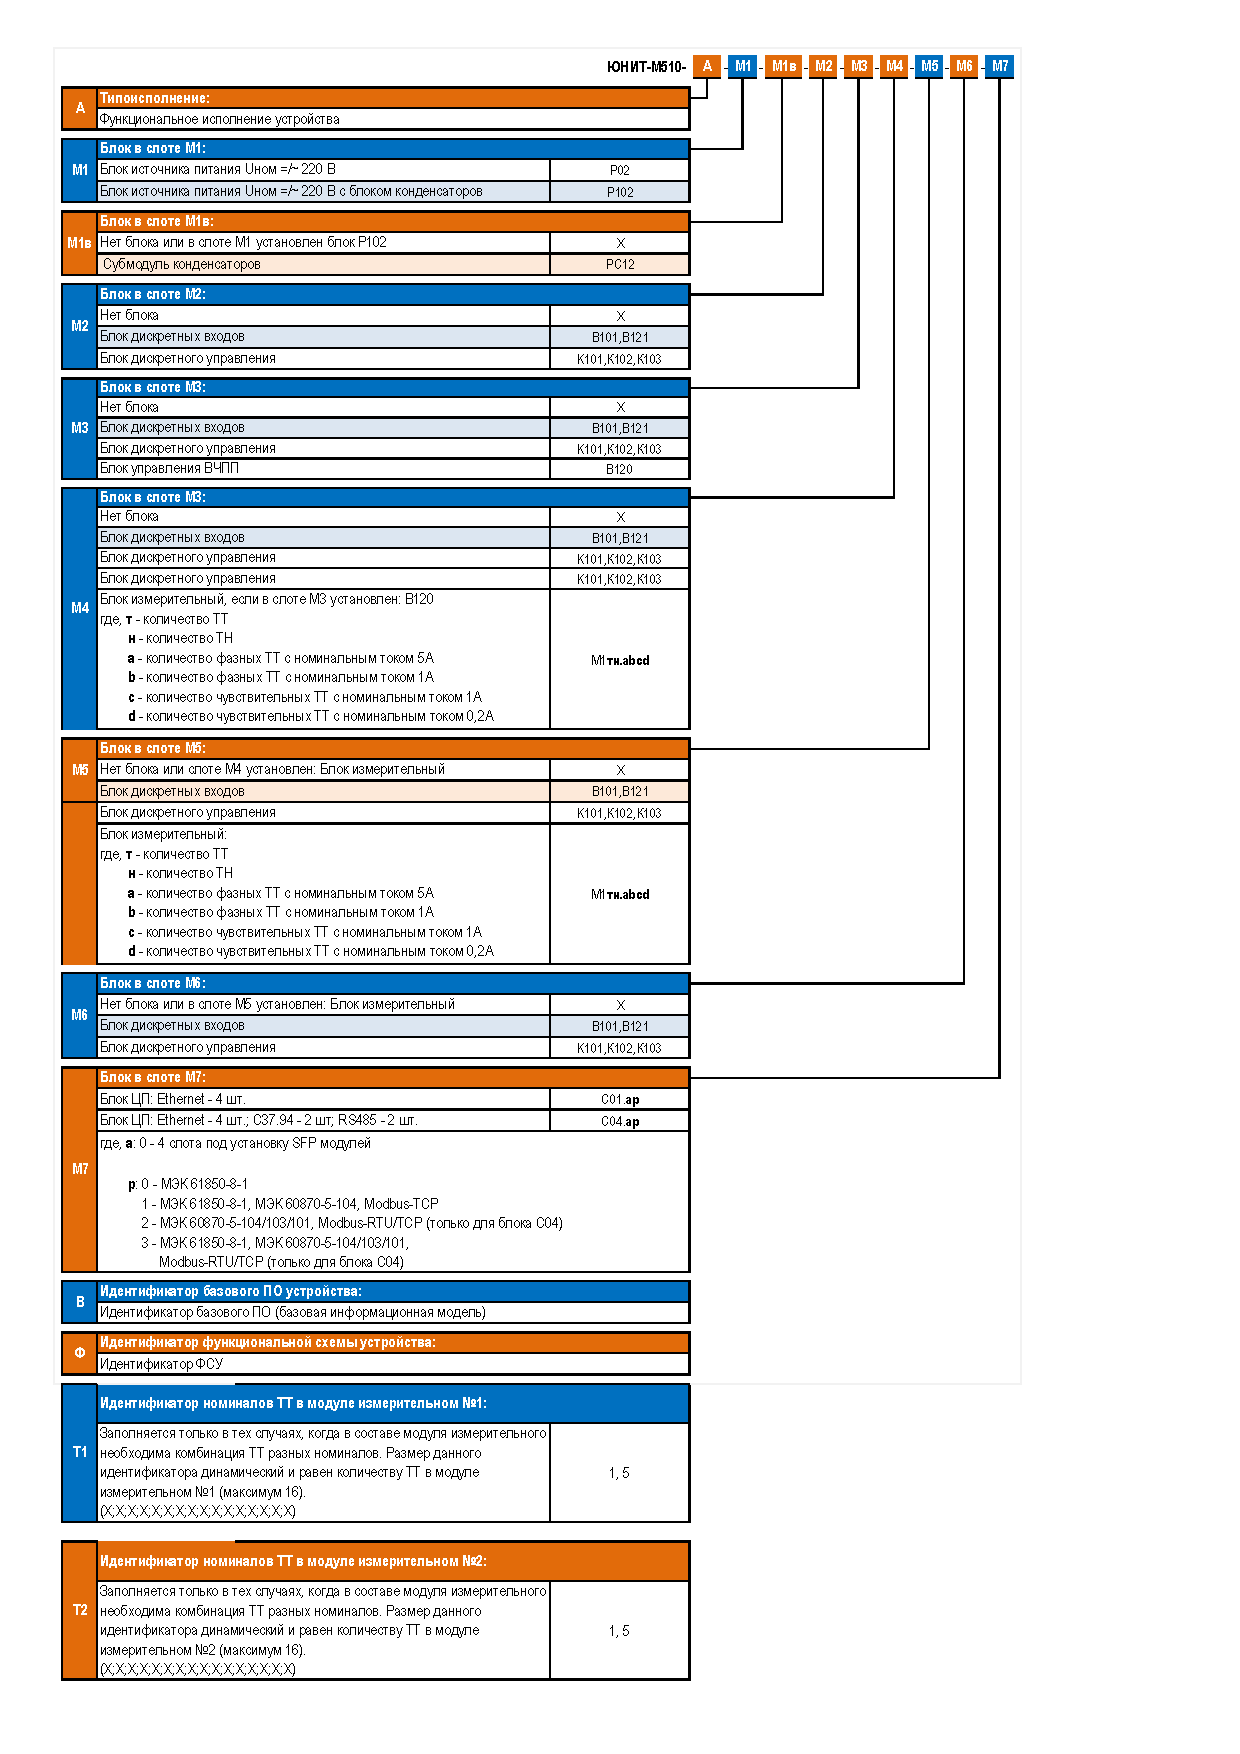
\includegraphics[width=0.9\textwidth,height=0.9\textheight,keepaspectratio]{img51.pdf}
  \captionof{figure}{Код заказа устройства «ЮНИТ-М510-ЛВ»}\label{appcard:img1}
 \end{figure}

 \begin{figure}[H]
  \centering
  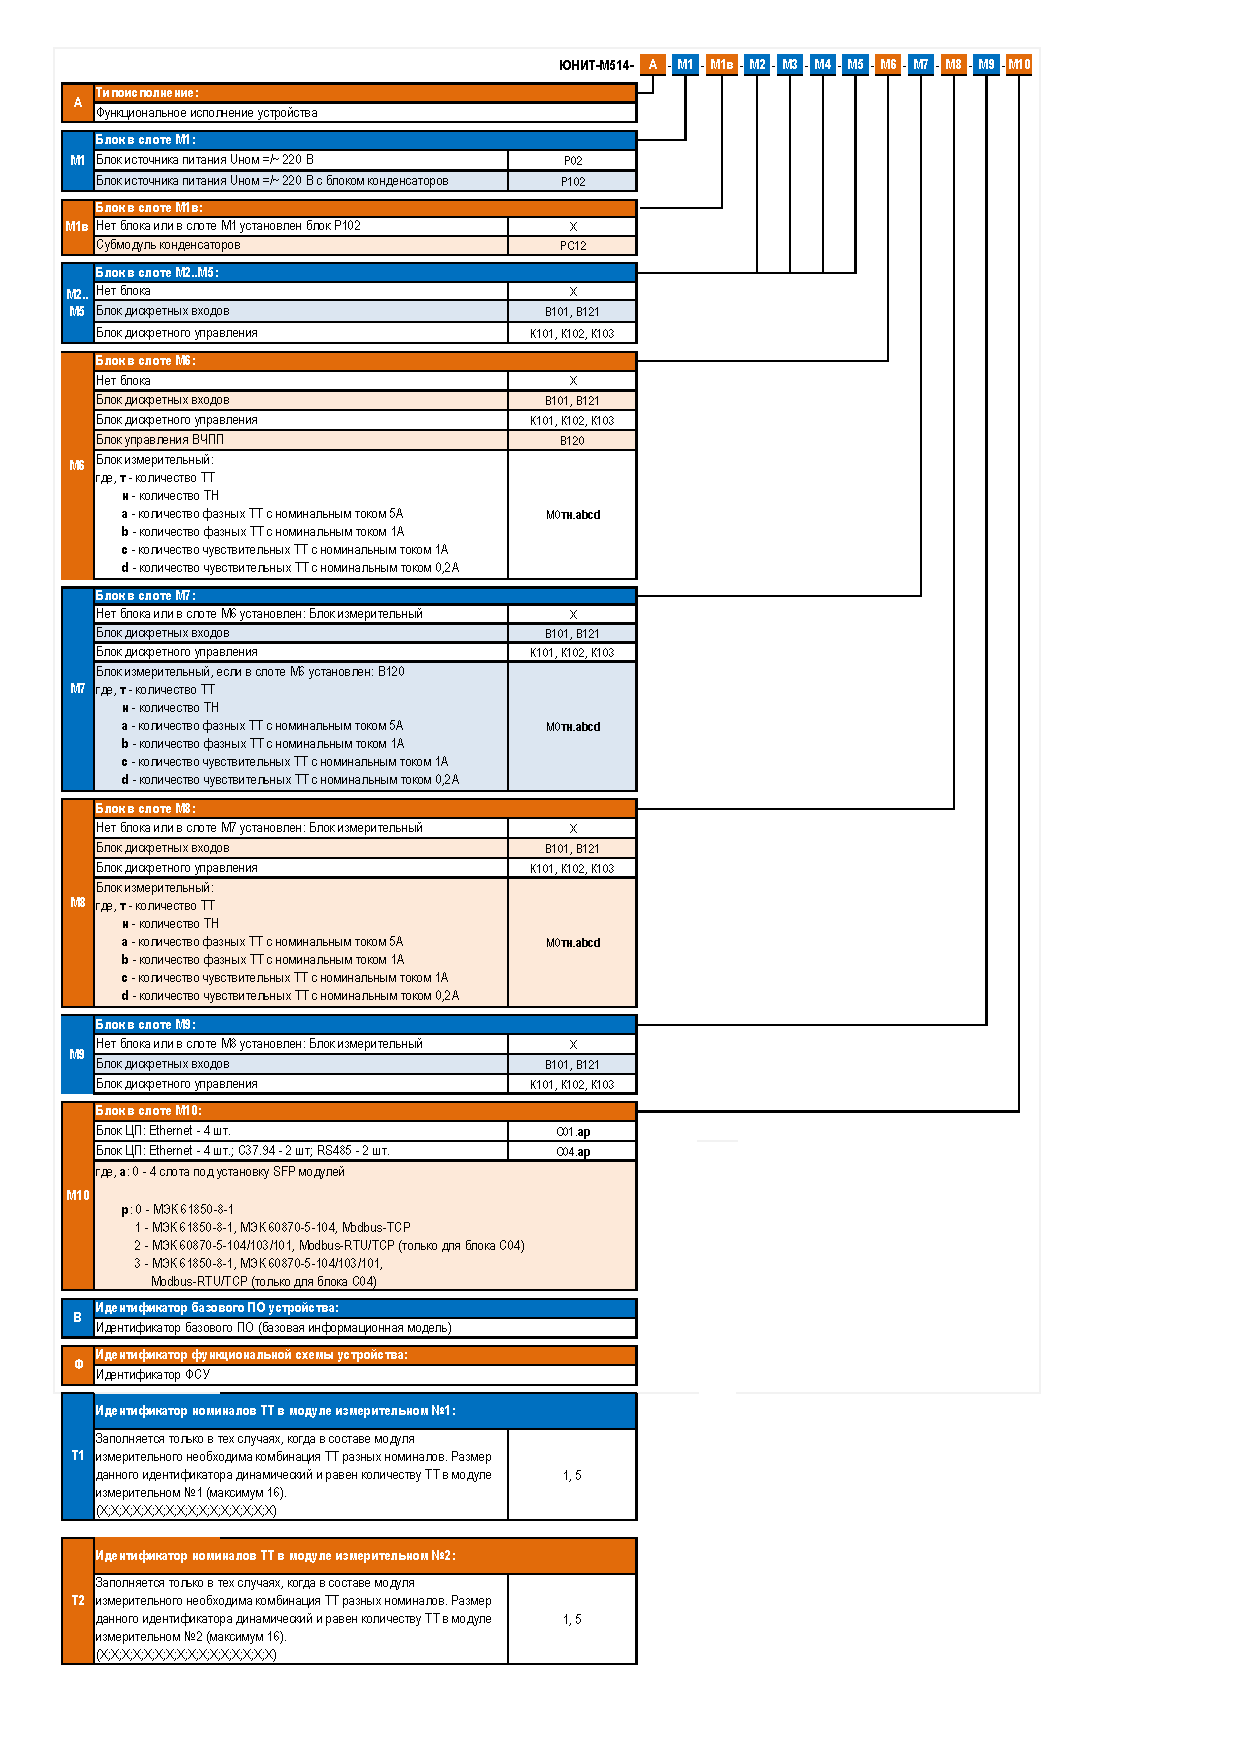
\includegraphics[width=1\textwidth,height=1\textheight,keepaspectratio]{img52.pdf}
  \captionof{figure}{Код заказа устройства «ЮНИТ-М514-ЛВ»}\label{appcard:img2}
 \end{figure}

 \begin{figure}[H]
  \centering
  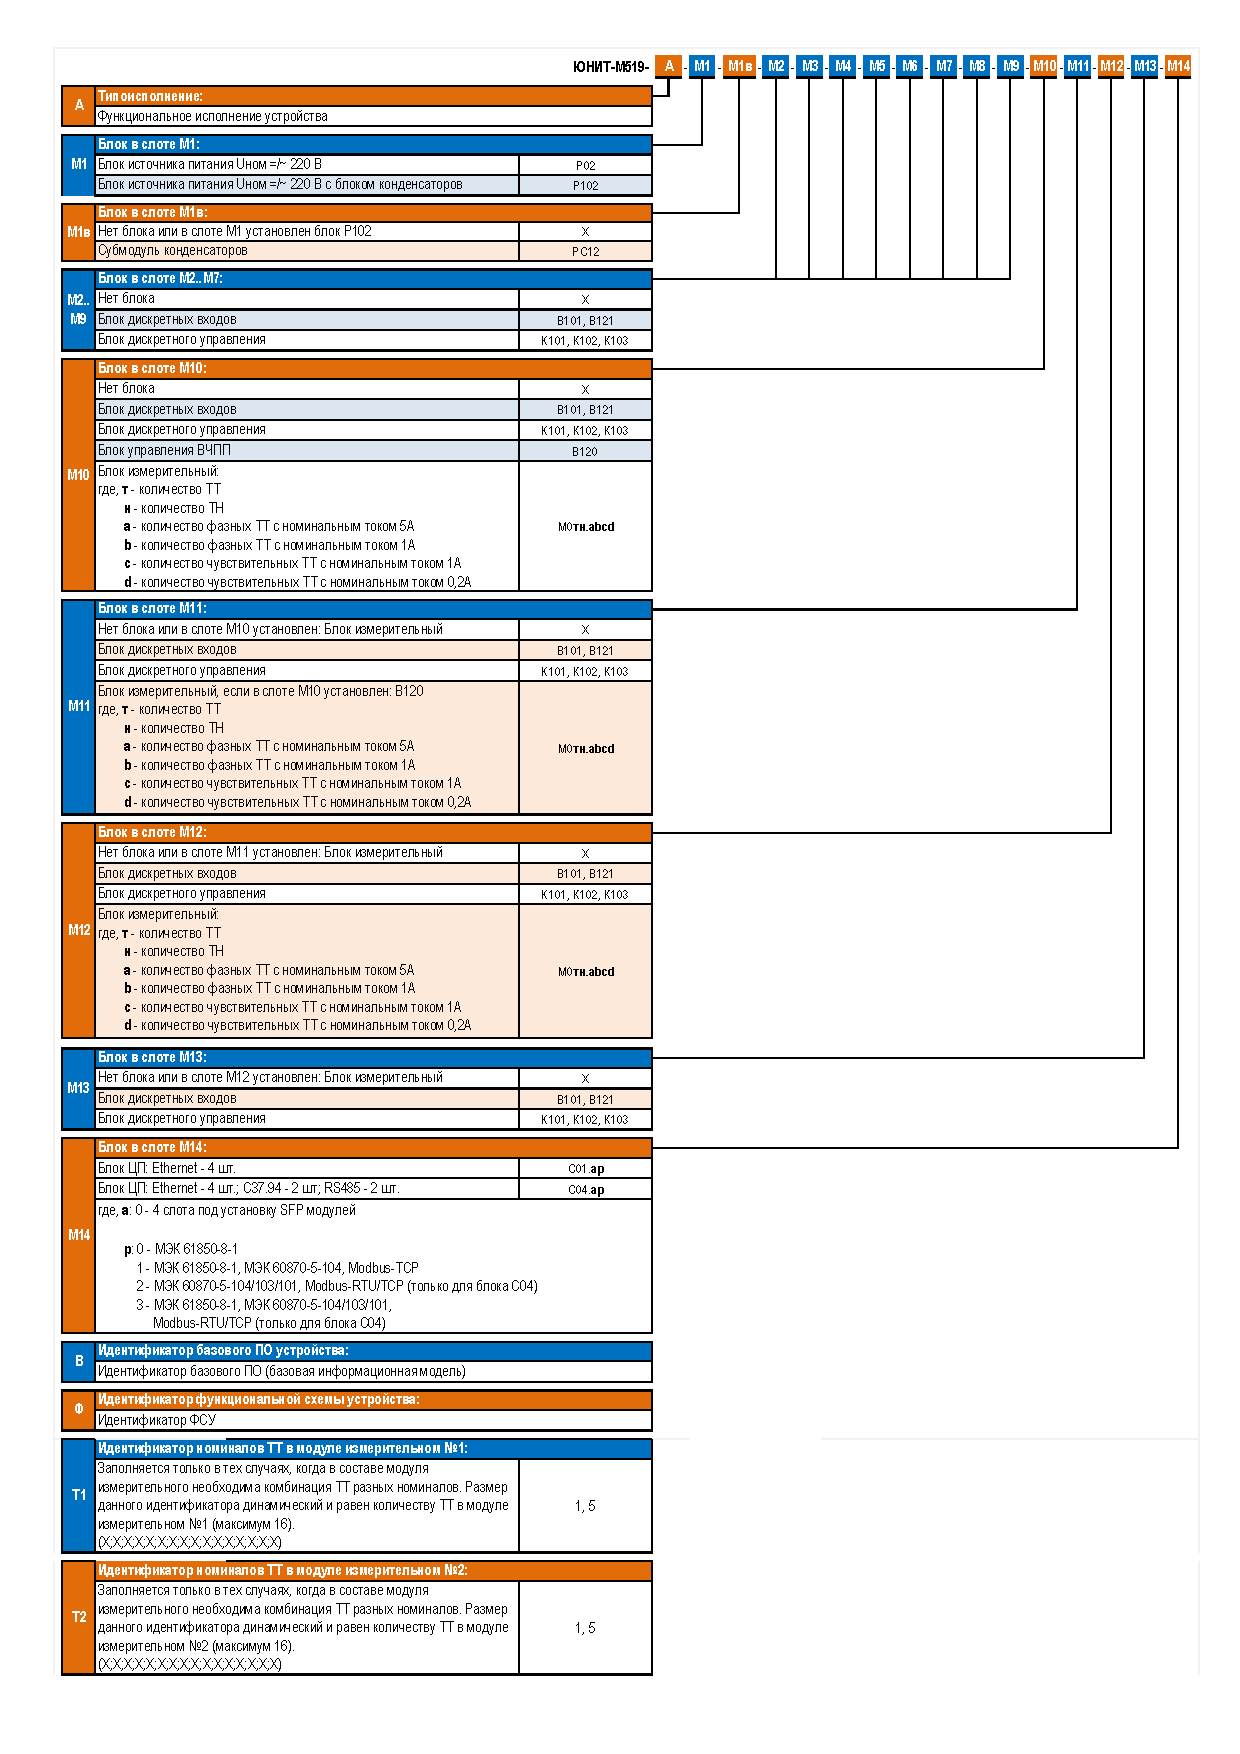
\includegraphics[width=1\textwidth,height=1\textheight,keepaspectratio]{img53.pdf}
  \captionof{figure}{Код заказа устройства «ЮНИТ-М519-ЛВ»}\label{appcard:img3}
 \end{figure}

\clearpage %!!!!!!!!!!БЕЗ ЭТОГО ХРЕНЬ\newpage
\newpage

\KOMAoptions{paper=A3,paper=landscape}
\areaset{390mm}{270mm}
\fancyheadoffset{0pt} % обновляем хедер и футер

\topmargin=-2.6cm % Команда \topmargin задаёт верхнее поле страницы. При этом поле отсчитывается не от левого края листа, а от линии, параллельной краю листа и отстоящей от него на 1 дюйм
\oddsidemargin=0cm % отступ слева https://zns.susu.ru/IT/latex/Marking/marking.html
\headsep=0cm
\footskip=-0.8cm
\setlength{\headheight}{1cm}

\color{unidarkgreen}{\section[(рекомендуемое) Структурно-функциональная схема устройства]{(рекомендуемое)\\Структурно-функциональная схема устройства}\label{app:fsu}}
\color{black}

\newcounter{filecounter}
\setcounter{filecounter}{0} % Начинаем с 0 , считаем что 0.pdf - лист с легендой и условными обозначениями
\loop
    \edef\filename{\apppath/Приложение. ФСУ/_latex/img/\arabic{filecounter}.pdf}
    \IfFileExists{\filename}{
        \begin{figure}[H]
        \centering
        \includegraphics[width=1\textwidth,height=1\textheight,keepaspectratio]{\filename}
        \end{figure}
        \clearpage
        \stepcounter{filecounter}
    }{\setcounter{filecounter}{0}} % условие выхода из цикла
    \ifnum\value{filecounter}>0
\repeat

\clearpage %!!!!!!!!!!БЕЗ ЭТОЙ СТРОЧКИ ХРЕНЬ



\newpage
\newpage
\newpage
\newpage
\newpage
\KOMAoption{paper}{a4, portrait}
\areaset{267mm}{180mm}
\fancyheadoffset{0pt} % обновляем хедер и футер

\newgeometry{
  top=14mm,
  bottom=11mm,
  right=10mm,
  left=22mm,
}

\begin{landscape}

\setlength{\footskip}{15.5pt}

\color{unidarkgreen}{\section[(справочное) Перечень сигналов ФСУ, предназначенных для \newline конфигурирования устройства «ЮНИТ-М300-ДЗТ2»]{(справочное)\\Перечень сигналов ФСУ, предназначенных для конфигурирования устройства «ЮНИТ-М300-ДЗТ2»}\label{app:signals}}
\color{black}

\begin{enumerate}[label=\ref{app:signals}.\arabic*] % Без глобального влияния
  \item Перечень сигналов самодиагностики, доступных для конфигурирования, приведен в документации ЮТКБ.656122.609 РЭ «Устройство защиты и автоматики серии «ЮНИТ-М300». Руководство по эксплуатации общее».
  \item Условные обозначения, применяемые в таблице перечня сигналов:
  \begin{itemize}
    \item[$\text{(--)}$] { - сигнал не имеет возможности конфигурации;}
    \item[$\text{(+)}$] { - сигнал имеет возможность конфигурации;}
    \item[$\text{(*)}$] { - конфигурация сигнала предустановлена по умолчанию в сервисном ПО «ЮНИТ-СЕРВИС» и не может быть изменена.}
  \end{itemize}
\end{enumerate}

\small % сделаем шрифт в таблице поменьше
\begin{longtable}{
>{\centering\arraybackslash}m{6.0cm}
|>{\centering\arraybackslash}m{3.45cm}
|>{\centering\arraybackslash}m{2cm}
|>{\centering\arraybackslash}m{2cm}
|>{\centering\arraybackslash}m{2cm}
|>{\centering\arraybackslash}m{2cm}
|>{\centering\arraybackslash}m{2cm}
|>{\centering\arraybackslash}m{2cm}
|>{\centering\arraybackslash}m{2.107cm}
}

\caption{Перечень сигналов ФСУ, предназначенных для конфигурирования устройства\hfill\vspace{-0.5\baselineskip}}\label{appA:tbl1}\\ 

\hline
\rowcolor{gray!30}
Полное наименование сигнала & Наименование сигнала на ФСУ & Дискретные входы & Выходные реле & Светодиоды & Функционал. клавиши & Регистратор событий & Аварийный осциллограф & Пуск авар. осциллографа \\ 
\hline
\endfirsthead
\caption*{\hspace{3pt}\emph{Продолжение таблицы \ref{appA:tbl1}\hfill\vspace{-0.5\baselineskip}}} \\ % сделано по ГОСТ 2.105 п.6.8.7
\hline
\rowcolor{gray!30}
Полное наименование сигнала & Наименование сигнала на ФСУ & Дискретные входы & Выходные реле & Светодиоды & Функционал. клавиши & Регистратор событий & Аварийный осциллограф & Пуск авар. осциллографа \\ 
\endhead

\endfoot

\endlastfoot

\multicolumn{9}{c}{\textbf{Общие сигналы функциональной логики}} \\
\hline
\rowcolor{gray!15}
\multicolumn{9}{c}{АПВ В1(ЛВ) ВН } \\
\hline
\multicolumn{9}{c}{\text{АПВ СШ}} \\
\hline
\raggedright АПВ В1(ЛВ) ВН/ АПВ СШ: Нет усл. вкл. & \centering АПВ В1(ЛВ) ВН/ АПВ СШ: Нет усл. вкл. & \centering -- & \centering -- & \centering -- & \centering -- & \centering -- & \centering -- & \centering \arraybackslash -- \\ \hline
\raggedright АПВ В1(ЛВ) ВН/ АПВ СШ: Выведено & \centering АПВ В1(ЛВ) ВН/ АПВ СШ: Выведено & \centering -- & \centering -- & \centering -- & \centering -- & \centering -- & \centering -- & \centering \arraybackslash -- \\ \hline
\raggedright АПВ В1(ЛВ) ВН/ АПВ СШ: Включить & \centering АПВ В1(ЛВ) ВН/ АПВ СШ: Включить & \centering -- & \centering -- & \centering -- & \centering -- & \centering -- & \centering -- & \centering \arraybackslash -- \\ \hline
\raggedright АПВ В1(ЛВ) ВН/ АПВ СШ: П. АПВш & \centering АПВ В1(ЛВ) ВН/ АПВ СШ: П. АПВш & \centering -- & \centering -- & \centering -- & \centering -- & \centering -- & \centering -- & \centering \arraybackslash -- \\ \hline
\raggedright АПВ В1(ЛВ) ВН/ АПВ СШ: Гот. АПВш & \centering АПВ В1(ЛВ) ВН/ АПВ СШ: Гот. АПВш & \centering -- & \centering -- & \centering -- & \centering -- & \centering -- & \centering -- & \centering \arraybackslash -- \\ \hline
\raggedright АПВ В1(ЛВ) ВН/ АПВ СШ: КЗ отключено & \centering АПВ В1(ЛВ) ВН/ АПВ СШ: КЗ отключено & \centering -- & \centering -- & \centering -- & \centering -- & \centering -- & \centering -- & \centering \arraybackslash -- \\ \hline
\raggedright АПВ В1(ЛВ) ВН/ АПВ СШ: В включен от АПВш & \centering АПВ В1(ЛВ) ВН/ АПВ СШ: В включен от АПВш & \centering -- & \centering -- & \centering -- & \centering -- & \centering -- & \centering -- & \centering \arraybackslash -- \\ \hline
\raggedright АПВ В1(ЛВ) ВН/ АПВ СШ: Успешное АПВл & \centering АПВ В1(ЛВ) ВН/ АПВ СШ: Успешное АПВл & \centering -- & \centering -- & \centering -- & \centering -- & \centering -- & \centering -- & \centering \arraybackslash -- \\ \hline
\raggedright АПВ В1(ЛВ) ВН/ АПВ СШ: Неуспешное АПВш & \centering АПВ В1(ЛВ) ВН/ АПВ СШ: Неуспешное АПВш & \centering -- & \centering -- & \centering -- & \centering -- & \centering -- & \centering -- & \centering \arraybackslash -- \\ \hline
\multicolumn{9}{c}{\text{АПВ Т}} \\
\hline
\raggedright АПВ В1(ЛВ) ВН/ АПВ Т: Режим без контролей & \centering АПВ В1(ЛВ) ВН/ АПВ Т: Режим без контролей & \centering -- & \centering -- & \centering -- & \centering -- & \centering -- & \centering -- & \centering \arraybackslash -- \\ \hline
\raggedright АПВ В1(ЛВ) ВН/ АПВ Т: Нет усл. вкл. & \centering АПВ В1(ЛВ) ВН/ АПВ Т: Нет усл. вкл. & \centering -- & \centering -- & \centering -- & \centering -- & \centering -- & \centering -- & \centering \arraybackslash -- \\ \hline
\raggedright АПВ В1(ЛВ) ВН/ АПВ Т: Ср. АПВт-1 & \centering АПВ В1(ЛВ) ВН/ АПВ Т: Ср. АПВт-1 & \centering -- & \centering -- & \centering -- & \centering -- & \centering -- & \centering -- & \centering \arraybackslash -- \\ \hline
\raggedright АПВ В1(ЛВ) ВН/ АПВ Т: Включить & \centering АПВ В1(ЛВ) ВН/ АПВ Т: Включить & \centering -- & \centering -- & \centering -- & \centering -- & \centering -- & \centering -- & \centering \arraybackslash -- \\ \hline
\raggedright АПВ В1(ЛВ) ВН/ АПВ Т: Ср. АПВт-2 & \centering АПВ В1(ЛВ) ВН/ АПВ Т: Ср. АПВт-2 & \centering -- & \centering -- & \centering -- & \centering -- & \centering -- & \centering -- & \centering \arraybackslash -- \\ \hline
\raggedright АПВ В1(ЛВ) ВН/ АПВ Т: Пуск АПВт-1 & \centering АПВ В1(ЛВ) ВН/ АПВ Т: Пуск АПВт-1 & \centering -- & \centering -- & \centering -- & \centering -- & \centering -- & \centering -- & \centering \arraybackslash -- \\ \hline
\raggedright АПВ В1(ЛВ) ВН/ АПВ Т: Пуск АПВт & \centering АПВ В1(ЛВ) ВН/ АПВ Т: Пуск АПВт & \centering -- & \centering -- & \centering -- & \centering -- & \centering -- & \centering -- & \centering \arraybackslash -- \\ \hline
\raggedright АПВ В1(ЛВ) ВН/ АПВ Т: Пуск АПВт-2 & \centering АПВ В1(ЛВ) ВН/ АПВ Т: Пуск АПВт-2 & \centering -- & \centering -- & \centering -- & \centering -- & \centering -- & \centering -- & \centering \arraybackslash -- \\ \hline
\raggedright АПВ В1(ЛВ) ВН/ АПВ Т: Гот. АПВт & \centering АПВ В1(ЛВ) ВН/ АПВ Т: Гот. АПВт & \centering -- & \centering -- & \centering -- & \centering -- & \centering -- & \centering -- & \centering \arraybackslash -- \\ \hline
\raggedright АПВ В1(ЛВ) ВН/ АПВ Т: Гот. АПВт-2 & \centering АПВ В1(ЛВ) ВН/ АПВ Т: Гот. АПВт-2 & \centering -- & \centering -- & \centering -- & \centering -- & \centering -- & \centering -- & \centering \arraybackslash -- \\ \hline
\raggedright АПВ В1(ЛВ) ВН/ АПВ Т: КЗ отключено & \centering АПВ В1(ЛВ) ВН/ АПВ Т: КЗ отключено & \centering -- & \centering -- & \centering -- & \centering -- & \centering -- & \centering -- & \centering \arraybackslash -- \\ \hline
\raggedright АПВ В1(ЛВ) ВН/ АПВ Т: В включен от АПВт & \centering АПВ В1(ЛВ) ВН/ АПВ Т: В включен от АПВт & \centering -- & \centering -- & \centering -- & \centering -- & \centering -- & \centering -- & \centering \arraybackslash -- \\ \hline
\raggedright АПВ В1(ЛВ) ВН/ АПВ Т: Успешное АПВт & \centering АПВ В1(ЛВ) ВН/ АПВ Т: Успешное АПВт & \centering -- & \centering -- & \centering -- & \centering -- & \centering -- & \centering -- & \centering \arraybackslash -- \\ \hline
\raggedright АПВ В1(ЛВ) ВН/ АПВ Т: Неуспешное АПВт & \centering АПВ В1(ЛВ) ВН/ АПВ Т: Неуспешное АПВт & \centering -- & \centering -- & \centering -- & \centering -- & \centering -- & \centering -- & \centering \arraybackslash -- \\ \hline
\raggedright АПВ В1(ЛВ) ВН/ АПВ Т: Неуспешное АПВт-1 & \centering АПВ В1(ЛВ) ВН/ АПВ Т: Неуспешное АПВт-1 & \centering -- & \centering -- & \centering -- & \centering -- & \centering -- & \centering -- & \centering \arraybackslash -- \\ \hline
\raggedright АПВ В1(ЛВ) ВН/ АПВ Т: Выведено & \centering АПВ В1(ЛВ) ВН/ АПВ Т: Выведено & \centering -- & \centering -- & \centering -- & \centering -- & \centering -- & \centering -- & \centering \arraybackslash -- \\ \hline
\rowcolor{gray!15}
\multicolumn{9}{c}{АПВ В1(ЛВ) СН } \\
\hline
\multicolumn{9}{c}{\text{АПВ СШ}} \\
\hline
\raggedright АПВ В1(ЛВ) СН/ АПВ СШ: Нет усл. вкл. & \centering АПВ В1(ЛВ) СН/ АПВ СШ: Нет усл. вкл. & \centering -- & \centering -- & \centering -- & \centering -- & \centering -- & \centering -- & \centering \arraybackslash -- \\ \hline
\raggedright АПВ В1(ЛВ) СН/ АПВ СШ: Включить & \centering АПВ В1(ЛВ) СН/ АПВ СШ: Включить & \centering -- & \centering -- & \centering -- & \centering -- & \centering -- & \centering -- & \centering \arraybackslash -- \\ \hline
\raggedright АПВ В1(ЛВ) СН/ АПВ СШ: П. АПВш & \centering АПВ В1(ЛВ) СН/ АПВ СШ: П. АПВш & \centering -- & \centering -- & \centering -- & \centering -- & \centering -- & \centering -- & \centering \arraybackslash -- \\ \hline
\raggedright АПВ В1(ЛВ) СН/ АПВ СШ: Гот. АПВш & \centering АПВ В1(ЛВ) СН/ АПВ СШ: Гот. АПВш & \centering -- & \centering -- & \centering -- & \centering -- & \centering -- & \centering -- & \centering \arraybackslash -- \\ \hline
\raggedright АПВ В1(ЛВ) СН/ АПВ СШ: КЗ отключено & \centering АПВ В1(ЛВ) СН/ АПВ СШ: КЗ отключено & \centering -- & \centering -- & \centering -- & \centering -- & \centering -- & \centering -- & \centering \arraybackslash -- \\ \hline
\raggedright АПВ В1(ЛВ) СН/ АПВ СШ: В включен от АПВш & \centering АПВ В1(ЛВ) СН/ АПВ СШ: В включен от АПВш & \centering -- & \centering -- & \centering -- & \centering -- & \centering -- & \centering -- & \centering \arraybackslash -- \\ \hline
\raggedright АПВ В1(ЛВ) СН/ АПВ СШ: Успешное АПВл & \centering АПВ В1(ЛВ) СН/ АПВ СШ: Успешное АПВл & \centering -- & \centering -- & \centering -- & \centering -- & \centering -- & \centering -- & \centering \arraybackslash -- \\ \hline
\raggedright АПВ В1(ЛВ) СН/ АПВ СШ: Неуспешное АПВш & \centering АПВ В1(ЛВ) СН/ АПВ СШ: Неуспешное АПВш & \centering -- & \centering -- & \centering -- & \centering -- & \centering -- & \centering -- & \centering \arraybackslash -- \\ \hline
\raggedright АПВ В1(ЛВ) СН/ АПВ СШ: Выведено & \centering АПВ В1(ЛВ) СН/ АПВ СШ: Выведено & \centering -- & \centering -- & \centering -- & \centering -- & \centering -- & \centering -- & \centering \arraybackslash -- \\ \hline
\multicolumn{9}{c}{\text{АПВ Т}} \\
\hline
\raggedright АПВ В1(ЛВ) СН/ АПВ Т: Режим без контролей & \centering АПВ В1(ЛВ) СН/ АПВ Т: Режим без контролей & \centering -- & \centering -- & \centering -- & \centering -- & \centering -- & \centering -- & \centering \arraybackslash -- \\ \hline
\raggedright АПВ В1(ЛВ) СН/ АПВ Т: Нет усл. вкл. & \centering АПВ В1(ЛВ) СН/ АПВ Т: Нет усл. вкл. & \centering -- & \centering -- & \centering -- & \centering -- & \centering -- & \centering -- & \centering \arraybackslash -- \\ \hline
\raggedright АПВ В1(ЛВ) СН/ АПВ Т: Ср. АПВт-1 & \centering АПВ В1(ЛВ) СН/ АПВ Т: Ср. АПВт-1 & \centering -- & \centering -- & \centering -- & \centering -- & \centering -- & \centering -- & \centering \arraybackslash -- \\ \hline
\raggedright АПВ В1(ЛВ) СН/ АПВ Т: Включить & \centering АПВ В1(ЛВ) СН/ АПВ Т: Включить & \centering -- & \centering -- & \centering -- & \centering -- & \centering -- & \centering -- & \centering \arraybackslash -- \\ \hline
\raggedright АПВ В1(ЛВ) СН/ АПВ Т: Ср. АПВт-2 & \centering АПВ В1(ЛВ) СН/ АПВ Т: Ср. АПВт-2 & \centering -- & \centering -- & \centering -- & \centering -- & \centering -- & \centering -- & \centering \arraybackslash -- \\ \hline
\raggedright АПВ В1(ЛВ) СН/ АПВ Т: Пуск АПВт-1 & \centering АПВ В1(ЛВ) СН/ АПВ Т: Пуск АПВт-1 & \centering -- & \centering -- & \centering -- & \centering -- & \centering -- & \centering -- & \centering \arraybackslash -- \\ \hline
\raggedright АПВ В1(ЛВ) СН/ АПВ Т: Пуск АПВт & \centering АПВ В1(ЛВ) СН/ АПВ Т: Пуск АПВт & \centering -- & \centering -- & \centering -- & \centering -- & \centering -- & \centering -- & \centering \arraybackslash -- \\ \hline
\raggedright АПВ В1(ЛВ) СН/ АПВ Т: Пуск АПВт-2 & \centering АПВ В1(ЛВ) СН/ АПВ Т: Пуск АПВт-2 & \centering -- & \centering -- & \centering -- & \centering -- & \centering -- & \centering -- & \centering \arraybackslash -- \\ \hline
\raggedright АПВ В1(ЛВ) СН/ АПВ Т: Гот. АПВт & \centering АПВ В1(ЛВ) СН/ АПВ Т: Гот. АПВт & \centering -- & \centering -- & \centering -- & \centering -- & \centering -- & \centering -- & \centering \arraybackslash -- \\ \hline
\raggedright АПВ В1(ЛВ) СН/ АПВ Т: Гот. АПВт-2 & \centering АПВ В1(ЛВ) СН/ АПВ Т: Гот. АПВт-2 & \centering -- & \centering -- & \centering -- & \centering -- & \centering -- & \centering -- & \centering \arraybackslash -- \\ \hline
\raggedright АПВ В1(ЛВ) СН/ АПВ Т: КЗ отключено & \centering АПВ В1(ЛВ) СН/ АПВ Т: КЗ отключено & \centering -- & \centering -- & \centering -- & \centering -- & \centering -- & \centering -- & \centering \arraybackslash -- \\ \hline
\raggedright АПВ В1(ЛВ) СН/ АПВ Т: В включен от АПВт & \centering АПВ В1(ЛВ) СН/ АПВ Т: В включен от АПВт & \centering -- & \centering -- & \centering -- & \centering -- & \centering -- & \centering -- & \centering \arraybackslash -- \\ \hline
\raggedright АПВ В1(ЛВ) СН/ АПВ Т: Успешное АПВт & \centering АПВ В1(ЛВ) СН/ АПВ Т: Успешное АПВт & \centering -- & \centering -- & \centering -- & \centering -- & \centering -- & \centering -- & \centering \arraybackslash -- \\ \hline
\raggedright АПВ В1(ЛВ) СН/ АПВ Т: Неуспешное АПВт & \centering АПВ В1(ЛВ) СН/ АПВ Т: Неуспешное АПВт & \centering -- & \centering -- & \centering -- & \centering -- & \centering -- & \centering -- & \centering \arraybackslash -- \\ \hline
\raggedright АПВ В1(ЛВ) СН/ АПВ Т: Неуспешное АПВт-1 & \centering АПВ В1(ЛВ) СН/ АПВ Т: Неуспешное АПВт-1 & \centering -- & \centering -- & \centering -- & \centering -- & \centering -- & \centering -- & \centering \arraybackslash -- \\ \hline
\raggedright АПВ В1(ЛВ) СН/ АПВ Т: Выведено & \centering АПВ В1(ЛВ) СН/ АПВ Т: Выведено & \centering -- & \centering -- & \centering -- & \centering -- & \centering -- & \centering -- & \centering \arraybackslash -- \\ \hline
\rowcolor{gray!15}
\multicolumn{9}{c}{БКУ В1(ЛВ) ВН } \\
\hline
\multicolumn{9}{c}{\text{БКУ}} \\
\hline
\raggedright БКУ В1(ЛВ) ВН/ БКУ: РКВ & \centering БКУ В1(ЛВ) ВН/ БКУ: РКВ & \centering -- & \centering -- & \centering -- & \centering -- & \centering -- & \centering -- & \centering \arraybackslash -- \\ \hline
\raggedright БКУ В1(ЛВ) ВН/ БКУ: РКО & \centering БКУ В1(ЛВ) ВН/ БКУ: РКО & \centering -- & \centering -- & \centering -- & \centering -- & \centering -- & \centering -- & \centering \arraybackslash -- \\ \hline
\rowcolor{gray!15}
\multicolumn{9}{c}{БКУ В1(ЛВ) СН } \\
\hline
\multicolumn{9}{c}{\text{БКУ}} \\
\hline
\raggedright БКУ В1(ЛВ) СН/ БКУ: РКВ & \centering БКУ В1(ЛВ) СН/ БКУ: РКВ & \centering -- & \centering -- & \centering -- & \centering -- & \centering -- & \centering -- & \centering \arraybackslash -- \\ \hline
\raggedright БКУ В1(ЛВ) СН/ БКУ: РКО & \centering БКУ В1(ЛВ) СН/ БКУ: РКО & \centering -- & \centering -- & \centering -- & \centering -- & \centering -- & \centering -- & \centering \arraybackslash -- \\ \hline
\rowcolor{gray!15}
\multicolumn{9}{c}{ГЗ РПН } \\
\hline
\multicolumn{9}{c}{ Общие сигналы блока } \\
\hline
\raggedright ГЗ РПН: Отключение & \centering ГЗ РПН: Отключение & \centering -- & \centering -- & \centering -- & \centering -- & \centering -- & \centering -- & \centering \arraybackslash -- \\ \hline
\raggedright ГЗ РПН: Срабатывание & \centering ГЗ РПН: Срабатывание & \centering -- & \centering -- & \centering -- & \centering -- & \centering -- & \centering -- & \centering \arraybackslash -- \\ \hline
\raggedright ГЗ РПН: Блокировка & \centering ГЗ РПН: Блокировка & \centering -- & \centering -- & \centering -- & \centering -- & \centering -- & \centering -- & \centering \arraybackslash -- \\ \hline
\raggedright ГЗ РПН: Неисправность & \centering ГЗ РПН: Неисправность & \centering -- & \centering -- & \centering -- & \centering -- & \centering -- & \centering -- & \centering \arraybackslash -- \\ \hline
\raggedright ГЗ РПН: Срабатывание ф.А & \centering ГЗ РПН: Срабатывание ф.А & \centering -- & \centering -- & \centering -- & \centering -- & \centering -- & \centering -- & \centering \arraybackslash -- \\ \hline
\raggedright ГЗ РПН: Отключение ф.А & \centering ГЗ РПН: Отключение ф.А & \centering -- & \centering -- & \centering -- & \centering -- & \centering -- & \centering -- & \centering \arraybackslash -- \\ \hline
\raggedright ГЗ РПН: Срабатывание ф.В & \centering ГЗ РПН: Срабатывание ф.В & \centering -- & \centering -- & \centering -- & \centering -- & \centering -- & \centering -- & \centering \arraybackslash -- \\ \hline
\raggedright ГЗ РПН: Отключение ф.В & \centering ГЗ РПН: Отключение ф.В & \centering -- & \centering -- & \centering -- & \centering -- & \centering -- & \centering -- & \centering \arraybackslash -- \\ \hline
\raggedright ГЗ РПН: Срабатывание ф.С & \centering ГЗ РПН: Срабатывание ф.С & \centering -- & \centering -- & \centering -- & \centering -- & \centering -- & \centering -- & \centering \arraybackslash -- \\ \hline
\raggedright ГЗ РПН: Отключение ф.С & \centering ГЗ РПН: Отключение ф.С & \centering -- & \centering -- & \centering -- & \centering -- & \centering -- & \centering -- & \centering \arraybackslash -- \\ \hline
\raggedright ГЗ РПН: Блокировка ф.А & \centering ГЗ РПН: Блокировка ф.А & \centering -- & \centering -- & \centering -- & \centering -- & \centering -- & \centering -- & \centering \arraybackslash -- \\ \hline
\raggedright ГЗ РПН: Блокировка ф.В & \centering ГЗ РПН: Блокировка ф.В & \centering -- & \centering -- & \centering -- & \centering -- & \centering -- & \centering -- & \centering \arraybackslash -- \\ \hline
\raggedright ГЗ РПН: Блокировка ф.С & \centering ГЗ РПН: Блокировка ф.С & \centering -- & \centering -- & \centering -- & \centering -- & \centering -- & \centering -- & \centering \arraybackslash -- \\ \hline
\raggedright ГЗ РПН: Неисправность ф.А & \centering ГЗ РПН: Неисправность ф.А & \centering -- & \centering -- & \centering -- & \centering -- & \centering -- & \centering -- & \centering \arraybackslash -- \\ \hline
\raggedright ГЗ РПН: Неисправность ф.В & \centering ГЗ РПН: Неисправность ф.В & \centering -- & \centering -- & \centering -- & \centering -- & \centering -- & \centering -- & \centering \arraybackslash -- \\ \hline
\raggedright ГЗ РПН: Неисправность ф.С & \centering ГЗ РПН: Неисправность ф.С & \centering -- & \centering -- & \centering -- & \centering -- & \centering -- & \centering -- & \centering \arraybackslash -- \\ \hline
\multicolumn{9}{c}{\text{ГЗ откл.фС 1 цепь}} \\
\hline
\raggedright ГЗ РПН/ ГЗ откл.фС 1 цепь: Срабатывание & \centering ГЗ РПН/ ГЗ откл.фС 1 цепь: Срабатывание & \centering -- & \centering -- & \centering -- & \centering -- & \centering -- & \centering -- & \centering \arraybackslash -- \\ \hline
\raggedright ГЗ РПН/ ГЗ откл.фС 1 цепь: Блокировка & \centering ГЗ РПН/ ГЗ откл.фС 1 цепь: Блокировка & \centering -- & \centering -- & \centering -- & \centering -- & \centering -- & \centering -- & \centering \arraybackslash -- \\ \hline
\raggedright ГЗ РПН/ ГЗ откл.фС 1 цепь: Неисправность & \centering ГЗ РПН/ ГЗ откл.фС 1 цепь: Неисправность & \centering -- & \centering -- & \centering -- & \centering -- & \centering -- & \centering -- & \centering \arraybackslash -- \\ \hline
\raggedright ГЗ РПН/ ГЗ откл.фС 1 цепь: Выведено & \centering ГЗ РПН/ ГЗ откл.фС 1 цепь: Выведено & \centering -- & \centering -- & \centering -- & \centering -- & \centering -- & \centering -- & \centering \arraybackslash -- \\ \hline
\multicolumn{9}{c}{\text{ГЗ откл.фС 2 цепь}} \\
\hline
\raggedright ГЗ РПН/ ГЗ откл.фС 2 цепь: Срабатывание & \centering ГЗ РПН/ ГЗ откл.фС 2 цепь: Срабатывание & \centering -- & \centering -- & \centering -- & \centering -- & \centering -- & \centering -- & \centering \arraybackslash -- \\ \hline
\raggedright ГЗ РПН/ ГЗ откл.фС 2 цепь: Блокировка & \centering ГЗ РПН/ ГЗ откл.фС 2 цепь: Блокировка & \centering -- & \centering -- & \centering -- & \centering -- & \centering -- & \centering -- & \centering \arraybackslash -- \\ \hline
\raggedright ГЗ РПН/ ГЗ откл.фС 2 цепь: Неисправность & \centering ГЗ РПН/ ГЗ откл.фС 2 цепь: Неисправность & \centering -- & \centering -- & \centering -- & \centering -- & \centering -- & \centering -- & \centering \arraybackslash -- \\ \hline
\raggedright ГЗ РПН/ ГЗ откл.фС 2 цепь: Выведено & \centering ГЗ РПН/ ГЗ откл.фС 2 цепь: Выведено & \centering -- & \centering -- & \centering -- & \centering -- & \centering -- & \centering -- & \centering \arraybackslash -- \\ \hline
\multicolumn{9}{c}{\text{ГЗ откл.фА 1 цепь}} \\
\hline
\raggedright ГЗ РПН/ ГЗ откл.фА 1 цепь: Срабатывание & \centering ГЗ РПН/ ГЗ откл.фА 1 цепь: Срабатывание & \centering -- & \centering -- & \centering -- & \centering -- & \centering -- & \centering -- & \centering \arraybackslash -- \\ \hline
\raggedright ГЗ РПН/ ГЗ откл.фА 1 цепь: Блокировка & \centering ГЗ РПН/ ГЗ откл.фА 1 цепь: Блокировка & \centering -- & \centering -- & \centering -- & \centering -- & \centering -- & \centering -- & \centering \arraybackslash -- \\ \hline
\raggedright ГЗ РПН/ ГЗ откл.фА 1 цепь: Неисправность & \centering ГЗ РПН/ ГЗ откл.фА 1 цепь: Неисправность & \centering -- & \centering -- & \centering -- & \centering -- & \centering -- & \centering -- & \centering \arraybackslash -- \\ \hline
\raggedright ГЗ РПН/ ГЗ откл.фА 1 цепь: Выведено & \centering ГЗ РПН/ ГЗ откл.фА 1 цепь: Выведено & \centering -- & \centering -- & \centering -- & \centering -- & \centering -- & \centering -- & \centering \arraybackslash -- \\ \hline
\multicolumn{9}{c}{\text{ГЗ откл.фА 2 цепь}} \\
\hline
\raggedright ГЗ РПН/ ГЗ откл.фА 2 цепь: Срабатывание & \centering ГЗ РПН/ ГЗ откл.фА 2 цепь: Срабатывание & \centering -- & \centering -- & \centering -- & \centering -- & \centering -- & \centering -- & \centering \arraybackslash -- \\ \hline
\raggedright ГЗ РПН/ ГЗ откл.фА 2 цепь: Блокировка & \centering ГЗ РПН/ ГЗ откл.фА 2 цепь: Блокировка & \centering -- & \centering -- & \centering -- & \centering -- & \centering -- & \centering -- & \centering \arraybackslash -- \\ \hline
\raggedright ГЗ РПН/ ГЗ откл.фА 2 цепь: Неисправность & \centering ГЗ РПН/ ГЗ откл.фА 2 цепь: Неисправность & \centering -- & \centering -- & \centering -- & \centering -- & \centering -- & \centering -- & \centering \arraybackslash -- \\ \hline
\raggedright ГЗ РПН/ ГЗ откл.фА 2 цепь: Выведено & \centering ГЗ РПН/ ГЗ откл.фА 2 цепь: Выведено & \centering -- & \centering -- & \centering -- & \centering -- & \centering -- & \centering -- & \centering \arraybackslash -- \\ \hline
\multicolumn{9}{c}{\text{ГЗ откл.фВ 1 цепь}} \\
\hline
\raggedright ГЗ РПН/ ГЗ откл.фВ 1 цепь: Срабатывание & \centering ГЗ РПН/ ГЗ откл.фВ 1 цепь: Срабатывание & \centering -- & \centering -- & \centering -- & \centering -- & \centering -- & \centering -- & \centering \arraybackslash -- \\ \hline
\raggedright ГЗ РПН/ ГЗ откл.фВ 1 цепь: Блокировка & \centering ГЗ РПН/ ГЗ откл.фВ 1 цепь: Блокировка & \centering -- & \centering -- & \centering -- & \centering -- & \centering -- & \centering -- & \centering \arraybackslash -- \\ \hline
\raggedright ГЗ РПН/ ГЗ откл.фВ 1 цепь: Неисправность & \centering ГЗ РПН/ ГЗ откл.фВ 1 цепь: Неисправность & \centering -- & \centering -- & \centering -- & \centering -- & \centering -- & \centering -- & \centering \arraybackslash -- \\ \hline
\raggedright ГЗ РПН/ ГЗ откл.фВ 1 цепь: Выведено & \centering ГЗ РПН/ ГЗ откл.фВ 1 цепь: Выведено & \centering -- & \centering -- & \centering -- & \centering -- & \centering -- & \centering -- & \centering \arraybackslash -- \\ \hline
\multicolumn{9}{c}{\text{ГЗ откл.фВ 2 цепь}} \\
\hline
\raggedright ГЗ РПН/ ГЗ откл.фВ 2 цепь: Срабатывание & \centering ГЗ РПН/ ГЗ откл.фВ 2 цепь: Срабатывание & \centering -- & \centering -- & \centering -- & \centering -- & \centering -- & \centering -- & \centering \arraybackslash -- \\ \hline
\raggedright ГЗ РПН/ ГЗ откл.фВ 2 цепь: Блокировка & \centering ГЗ РПН/ ГЗ откл.фВ 2 цепь: Блокировка & \centering -- & \centering -- & \centering -- & \centering -- & \centering -- & \centering -- & \centering \arraybackslash -- \\ \hline
\raggedright ГЗ РПН/ ГЗ откл.фВ 2 цепь: Неисправность & \centering ГЗ РПН/ ГЗ откл.фВ 2 цепь: Неисправность & \centering -- & \centering -- & \centering -- & \centering -- & \centering -- & \centering -- & \centering \arraybackslash -- \\ \hline
\raggedright ГЗ РПН/ ГЗ откл.фВ 2 цепь: Выведено & \centering ГЗ РПН/ ГЗ откл.фВ 2 цепь: Выведено & \centering -- & \centering -- & \centering -- & \centering -- & \centering -- & \centering -- & \centering \arraybackslash -- \\ \hline
\rowcolor{gray!15}
\multicolumn{9}{c}{ГЗ АТ откл } \\
\hline
\multicolumn{9}{c}{ Общие сигналы блока } \\
\hline
\raggedright ГЗ АТ откл: Отключение & \centering ГЗ АТ откл: Отключение & \centering -- & \centering -- & \centering -- & \centering -- & \centering -- & \centering -- & \centering \arraybackslash -- \\ \hline
\raggedright ГЗ АТ откл: Срабатывание & \centering ГЗ АТ откл: Срабатывание & \centering -- & \centering -- & \centering -- & \centering -- & \centering -- & \centering -- & \centering \arraybackslash -- \\ \hline
\raggedright ГЗ АТ откл: Блокировка & \centering ГЗ АТ откл: Блокировка & \centering -- & \centering -- & \centering -- & \centering -- & \centering -- & \centering -- & \centering \arraybackslash -- \\ \hline
\raggedright ГЗ АТ откл: Неисправность & \centering ГЗ АТ откл: Неисправность & \centering -- & \centering -- & \centering -- & \centering -- & \centering -- & \centering -- & \centering \arraybackslash -- \\ \hline
\multicolumn{9}{c}{\text{ГЗ откл 1 цепь}} \\
\hline
\raggedright ГЗ АТ откл/ ГЗ откл 1 цепь: Срабатывание & \centering ГЗ АТ откл/ ГЗ откл 1 цепь: Срабатывание & \centering -- & \centering -- & \centering -- & \centering -- & \centering -- & \centering -- & \centering \arraybackslash -- \\ \hline
\raggedright ГЗ АТ откл/ ГЗ откл 1 цепь: Блокировка & \centering ГЗ АТ откл/ ГЗ откл 1 цепь: Блокировка & \centering -- & \centering -- & \centering -- & \centering -- & \centering -- & \centering -- & \centering \arraybackslash -- \\ \hline
\raggedright ГЗ АТ откл/ ГЗ откл 1 цепь: Неисправность & \centering ГЗ АТ откл/ ГЗ откл 1 цепь: Неисправность & \centering -- & \centering -- & \centering -- & \centering -- & \centering -- & \centering -- & \centering \arraybackslash -- \\ \hline
\raggedright ГЗ АТ откл/ ГЗ откл 1 цепь: Выведено & \centering ГЗ АТ откл/ ГЗ откл 1 цепь: Выведено & \centering -- & \centering -- & \centering -- & \centering -- & \centering -- & \centering -- & \centering \arraybackslash -- \\ \hline
\multicolumn{9}{c}{\text{ГЗ откл 2 цепь}} \\
\hline
\raggedright ГЗ АТ откл/ ГЗ откл 2 цепь: Срабатывание & \centering ГЗ АТ откл/ ГЗ откл 2 цепь: Срабатывание & \centering -- & \centering -- & \centering -- & \centering -- & \centering -- & \centering -- & \centering \arraybackslash -- \\ \hline
\raggedright ГЗ АТ откл/ ГЗ откл 2 цепь: Блокировка & \centering ГЗ АТ откл/ ГЗ откл 2 цепь: Блокировка & \centering -- & \centering -- & \centering -- & \centering -- & \centering -- & \centering -- & \centering \arraybackslash -- \\ \hline
\raggedright ГЗ АТ откл/ ГЗ откл 2 цепь: Неисправность & \centering ГЗ АТ откл/ ГЗ откл 2 цепь: Неисправность & \centering -- & \centering -- & \centering -- & \centering -- & \centering -- & \centering -- & \centering \arraybackslash -- \\ \hline
\raggedright ГЗ АТ откл/ ГЗ откл 2 цепь: Выведено & \centering ГЗ АТ откл/ ГЗ откл 2 цепь: Выведено & \centering -- & \centering -- & \centering -- & \centering -- & \centering -- & \centering -- & \centering \arraybackslash -- \\ \hline
\rowcolor{gray!15}
\multicolumn{9}{c}{ГЗ ЛРТ откл } \\
\hline
\multicolumn{9}{c}{ Общие сигналы блока } \\
\hline
\raggedright ГЗ ЛРТ откл: Отключение & \centering ГЗ ЛРТ откл: Отключение & \centering -- & \centering -- & \centering -- & \centering -- & \centering -- & \centering -- & \centering \arraybackslash -- \\ \hline
\raggedright ГЗ ЛРТ откл: Срабатывание & \centering ГЗ ЛРТ откл: Срабатывание & \centering -- & \centering -- & \centering -- & \centering -- & \centering -- & \centering -- & \centering \arraybackslash -- \\ \hline
\raggedright ГЗ ЛРТ откл: Блокировка & \centering ГЗ ЛРТ откл: Блокировка & \centering -- & \centering -- & \centering -- & \centering -- & \centering -- & \centering -- & \centering \arraybackslash -- \\ \hline
\raggedright ГЗ ЛРТ откл: Неисправность & \centering ГЗ ЛРТ откл: Неисправность & \centering -- & \centering -- & \centering -- & \centering -- & \centering -- & \centering -- & \centering \arraybackslash -- \\ \hline
\multicolumn{9}{c}{\text{ГЗ откл 1 цепь}} \\
\hline
\raggedright ГЗ ЛРТ откл/ ГЗ откл 1 цепь: Срабатывание & \centering ГЗ ЛРТ откл/ ГЗ откл 1 цепь: Срабатывание & \centering -- & \centering -- & \centering -- & \centering -- & \centering -- & \centering -- & \centering \arraybackslash -- \\ \hline
\raggedright ГЗ ЛРТ откл/ ГЗ откл 1 цепь: Блокировка & \centering ГЗ ЛРТ откл/ ГЗ откл 1 цепь: Блокировка & \centering -- & \centering -- & \centering -- & \centering -- & \centering -- & \centering -- & \centering \arraybackslash -- \\ \hline
\raggedright ГЗ ЛРТ откл/ ГЗ откл 1 цепь: Неисправность & \centering ГЗ ЛРТ откл/ ГЗ откл 1 цепь: Неисправность & \centering -- & \centering -- & \centering -- & \centering -- & \centering -- & \centering -- & \centering \arraybackslash -- \\ \hline
\raggedright ГЗ ЛРТ откл/ ГЗ откл 1 цепь: Выведено & \centering ГЗ ЛРТ откл/ ГЗ откл 1 цепь: Выведено & \centering -- & \centering -- & \centering -- & \centering -- & \centering -- & \centering -- & \centering \arraybackslash -- \\ \hline
\multicolumn{9}{c}{\text{ГЗ откл 2 цепь}} \\
\hline
\raggedright ГЗ ЛРТ откл/ ГЗ откл 2 цепь: Срабатывание & \centering ГЗ ЛРТ откл/ ГЗ откл 2 цепь: Срабатывание & \centering -- & \centering -- & \centering -- & \centering -- & \centering -- & \centering -- & \centering \arraybackslash -- \\ \hline
\raggedright ГЗ ЛРТ откл/ ГЗ откл 2 цепь: Блокировка & \centering ГЗ ЛРТ откл/ ГЗ откл 2 цепь: Блокировка & \centering -- & \centering -- & \centering -- & \centering -- & \centering -- & \centering -- & \centering \arraybackslash -- \\ \hline
\raggedright ГЗ ЛРТ откл/ ГЗ откл 2 цепь: Неисправность & \centering ГЗ ЛРТ откл/ ГЗ откл 2 цепь: Неисправность & \centering -- & \centering -- & \centering -- & \centering -- & \centering -- & \centering -- & \centering \arraybackslash -- \\ \hline
\raggedright ГЗ ЛРТ откл/ ГЗ откл 2 цепь: Выведено & \centering ГЗ ЛРТ откл/ ГЗ откл 2 цепь: Выведено & \centering -- & \centering -- & \centering -- & \centering -- & \centering -- & \centering -- & \centering \arraybackslash -- \\ \hline
\rowcolor{gray!15}
\multicolumn{9}{c}{ГЗ АТ сигн } \\
\hline
\multicolumn{9}{c}{ Общие сигналы блока } \\
\hline
\raggedright ГЗ АТ сигн: Срабатывание & \centering ГЗ АТ сигн: Срабатывание & \centering -- & \centering -- & \centering -- & \centering -- & \centering -- & \centering -- & \centering \arraybackslash -- \\ \hline
\raggedright ГЗ АТ сигн: Отключение & \centering ГЗ АТ сигн: Отключение & \centering -- & \centering -- & \centering -- & \centering -- & \centering -- & \centering -- & \centering \arraybackslash -- \\ \hline
\multicolumn{9}{c}{\text{ГЗ сигн 1 цепь}} \\
\hline
\raggedright ГЗ АТ сигн/ ГЗ сигн 1 цепь: Срабатывание & \centering ГЗ АТ сигн/ ГЗ сигн 1 цепь: Срабатывание & \centering -- & \centering -- & \centering -- & \centering -- & \centering -- & \centering -- & \centering \arraybackslash -- \\ \hline
\raggedright ГЗ АТ сигн/ ГЗ сигн 1 цепь: Выведено & \centering ГЗ АТ сигн/ ГЗ сигн 1 цепь: Выведено & \centering -- & \centering -- & \centering -- & \centering -- & \centering -- & \centering -- & \centering \arraybackslash -- \\ \hline
\multicolumn{9}{c}{\text{ГЗ сигн 2 цепь}} \\
\hline
\raggedright ГЗ АТ сигн/ ГЗ сигн 2 цепь: Срабатывание & \centering ГЗ АТ сигн/ ГЗ сигн 2 цепь: Срабатывание & \centering -- & \centering -- & \centering -- & \centering -- & \centering -- & \centering -- & \centering \arraybackslash -- \\ \hline
\raggedright ГЗ АТ сигн/ ГЗ сигн 2 цепь: Выведено & \centering ГЗ АТ сигн/ ГЗ сигн 2 цепь: Выведено & \centering -- & \centering -- & \centering -- & \centering -- & \centering -- & \centering -- & \centering \arraybackslash -- \\ \hline
\rowcolor{gray!15}
\multicolumn{9}{c}{ГЗ ЛРТ сигн } \\
\hline
\multicolumn{9}{c}{ Общие сигналы блока } \\
\hline
\raggedright ГЗ ЛРТ сигн: Отключение & \centering ГЗ ЛРТ сигн: Отключение & \centering -- & \centering -- & \centering -- & \centering -- & \centering -- & \centering -- & \centering \arraybackslash -- \\ \hline
\raggedright ГЗ ЛРТ сигн: Срабатывание & \centering ГЗ ЛРТ сигн: Срабатывание & \centering -- & \centering -- & \centering -- & \centering -- & \centering -- & \centering -- & \centering \arraybackslash -- \\ \hline
\multicolumn{9}{c}{\text{ГЗ сигн 1 цепь}} \\
\hline
\raggedright ГЗ ЛРТ сигн/ ГЗ сигн 1 цепь: Срабатывание & \centering ГЗ ЛРТ сигн/ ГЗ сигн 1 цепь: Срабатывание & \centering -- & \centering -- & \centering -- & \centering -- & \centering -- & \centering -- & \centering \arraybackslash -- \\ \hline
\raggedright ГЗ ЛРТ сигн/ ГЗ сигн 1 цепь: Выведено & \centering ГЗ ЛРТ сигн/ ГЗ сигн 1 цепь: Выведено & \centering -- & \centering -- & \centering -- & \centering -- & \centering -- & \centering -- & \centering \arraybackslash -- \\ \hline
\multicolumn{9}{c}{\text{ГЗ сигн 2 цепь}} \\
\hline
\raggedright ГЗ ЛРТ сигн/ ГЗ сигн 2 цепь: Срабатывание & \centering ГЗ ЛРТ сигн/ ГЗ сигн 2 цепь: Срабатывание & \centering -- & \centering -- & \centering -- & \centering -- & \centering -- & \centering -- & \centering \arraybackslash -- \\ \hline
\raggedright ГЗ ЛРТ сигн/ ГЗ сигн 2 цепь: Выведено & \centering ГЗ ЛРТ сигн/ ГЗ сигн 2 цепь: Выведено & \centering -- & \centering -- & \centering -- & \centering -- & \centering -- & \centering -- & \centering \arraybackslash -- \\ \hline
\rowcolor{gray!15}
\multicolumn{9}{c}{ДТЗ } \\
\hline
\multicolumn{9}{c}{ Общие сигналы блока } \\
\hline
\raggedright ДТЗ: Срабатывание фА & \centering ДТЗ: Срабатывание фА & \centering -- & \centering -- & \centering -- & \centering -- & \centering -- & \centering -- & \centering \arraybackslash -- \\ \hline
\raggedright ДТЗ: Срабатывание фВ & \centering ДТЗ: Срабатывание фВ & \centering -- & \centering -- & \centering -- & \centering -- & \centering -- & \centering -- & \centering \arraybackslash -- \\ \hline
\raggedright ДТЗ: Срабатывание фС & \centering ДТЗ: Срабатывание фС & \centering -- & \centering -- & \centering -- & \centering -- & \centering -- & \centering -- & \centering \arraybackslash -- \\ \hline
\raggedright ДТЗ: Срабатывание & \centering ДТЗ: Срабатывание & \centering -- & \centering -- & \centering -- & \centering -- & \centering -- & \centering -- & \centering \arraybackslash -- \\ \hline
\multicolumn{9}{c}{\text{Д2г}} \\
\hline
\raggedright ДТЗ/ Д2г: Срабатывание фA & \centering ДТЗ/ Д2г: Срабатывание фA & \centering -- & \centering -- & \centering -- & \centering -- & \centering -- & \centering -- & \centering \arraybackslash -- \\ \hline
\raggedright ДТЗ/ Д2г: Срабатывание фB & \centering ДТЗ/ Д2г: Срабатывание фB & \centering -- & \centering -- & \centering -- & \centering -- & \centering -- & \centering -- & \centering \arraybackslash -- \\ \hline
\raggedright ДТЗ/ Д2г: Срабатывание фC & \centering ДТЗ/ Д2г: Срабатывание фC & \centering -- & \centering -- & \centering -- & \centering -- & \centering -- & \centering -- & \centering \arraybackslash -- \\ \hline
\raggedright ДТЗ/ Д2г: Выведено & \centering ДТЗ/ Д2г: Выведено & \centering -- & \centering -- & \centering -- & \centering -- & \centering -- & \centering -- & \centering \arraybackslash -- \\ \hline
\multicolumn{9}{c}{\text{Д5г}} \\
\hline
\raggedright ДТЗ/ Д5г: Срабатывание фA & \centering ДТЗ/ Д5г: Срабатывание фA & \centering -- & \centering -- & \centering -- & \centering -- & \centering -- & \centering -- & \centering \arraybackslash -- \\ \hline
\raggedright ДТЗ/ Д5г: Срабатывание фB & \centering ДТЗ/ Д5г: Срабатывание фB & \centering -- & \centering -- & \centering -- & \centering -- & \centering -- & \centering -- & \centering \arraybackslash -- \\ \hline
\raggedright ДТЗ/ Д5г: Срабатывание фC & \centering ДТЗ/ Д5г: Срабатывание фC & \centering -- & \centering -- & \centering -- & \centering -- & \centering -- & \centering -- & \centering \arraybackslash -- \\ \hline
\raggedright ДТЗ/ Д5г: Выведено & \centering ДТЗ/ Д5г: Выведено & \centering -- & \centering -- & \centering -- & \centering -- & \centering -- & \centering -- & \centering \arraybackslash -- \\ \hline
\multicolumn{9}{c}{\text{ДТЗт}} \\
\hline
\raggedright ДТЗ/ ДТЗт: Срабатывание фА & \centering ДТЗ/ ДТЗт: Срабатывание фА & \centering -- & \centering -- & \centering -- & \centering -- & \centering -- & \centering -- & \centering \arraybackslash -- \\ \hline
\raggedright ДТЗ/ ДТЗт: ИО фB & \centering ДТЗ/ ДТЗт: ИО фB & \centering -- & \centering -- & \centering -- & \centering -- & \centering -- & \centering -- & \centering \arraybackslash -- \\ \hline
\raggedright ДТЗ/ ДТЗт: Срабатывание фB & \centering ДТЗ/ ДТЗт: Срабатывание фB & \centering -- & \centering -- & \centering -- & \centering -- & \centering -- & \centering -- & \centering \arraybackslash -- \\ \hline
\raggedright ДТЗ/ ДТЗт: ИО фC & \centering ДТЗ/ ДТЗт: ИО фC & \centering -- & \centering -- & \centering -- & \centering -- & \centering -- & \centering -- & \centering \arraybackslash -- \\ \hline
\raggedright ДТЗ/ ДТЗт: Срабатывание фC & \centering ДТЗ/ ДТЗт: Срабатывание фC & \centering -- & \centering -- & \centering -- & \centering -- & \centering -- & \centering -- & \centering \arraybackslash -- \\ \hline
\raggedright ДТЗ/ ДТЗт: Выведено & \centering ДТЗ/ ДТЗт: Выведено & \centering -- & \centering -- & \centering -- & \centering -- & \centering -- & \centering -- & \centering \arraybackslash -- \\ \hline
\raggedright ДТЗ/ ДТЗт: ИО фА & \centering ДТЗ/ ДТЗт: ИО фА & \centering -- & \centering -- & \centering -- & \centering -- & \centering -- & \centering -- & \centering \arraybackslash -- \\ \hline
\multicolumn{9}{c}{\text{ДТО}} \\
\hline
\raggedright ДТЗ/ ДТО: ИО фА & \centering ДТЗ/ ДТО: ИО фА & \centering -- & \centering -- & \centering -- & \centering -- & \centering -- & \centering -- & \centering \arraybackslash -- \\ \hline
\raggedright ДТЗ/ ДТО: Срабатывание фА & \centering ДТЗ/ ДТО: Срабатывание фА & \centering -- & \centering -- & \centering -- & \centering -- & \centering -- & \centering -- & \centering \arraybackslash -- \\ \hline
\raggedright ДТЗ/ ДТО: ИО фB & \centering ДТЗ/ ДТО: ИО фB & \centering -- & \centering -- & \centering -- & \centering -- & \centering -- & \centering -- & \centering \arraybackslash -- \\ \hline
\raggedright ДТЗ/ ДТО: Срабатывание фB & \centering ДТЗ/ ДТО: Срабатывание фB & \centering -- & \centering -- & \centering -- & \centering -- & \centering -- & \centering -- & \centering \arraybackslash -- \\ \hline
\raggedright ДТЗ/ ДТО: ИО фC & \centering ДТЗ/ ДТО: ИО фC & \centering -- & \centering -- & \centering -- & \centering -- & \centering -- & \centering -- & \centering \arraybackslash -- \\ \hline
\raggedright ДТЗ/ ДТО: Срабатывание фC & \centering ДТЗ/ ДТО: Срабатывание фC & \centering -- & \centering -- & \centering -- & \centering -- & \centering -- & \centering -- & \centering \arraybackslash -- \\ \hline
\raggedright ДТЗ/ ДТО: Выведено & \centering ДТЗ/ ДТО: Выведено & \centering -- & \centering -- & \centering -- & \centering -- & \centering -- & \centering -- & \centering \arraybackslash -- \\ \hline
\multicolumn{9}{c}{\text{КЦТ}} \\
\hline
\raggedright ДТЗ/ КЦТ: Срабатывание & \centering ДТЗ/ КЦТ: Срабатывание & \centering -- & \centering -- & \centering -- & \centering -- & \centering -- & \centering -- & \centering \arraybackslash -- \\ \hline
\rowcolor{gray!15}
\multicolumn{9}{c}{ЗП } \\
\hline
\multicolumn{9}{c}{ Общие сигналы блока } \\
\hline
\raggedright ЗП: Срабатывание & \centering ЗП: Срабатывание & \centering -- & \centering -- & \centering -- & \centering -- & \centering -- & \centering -- & \centering \arraybackslash -- \\ \hline
\raggedright ЗП: Пуск & \centering ЗП: Пуск & \centering -- & \centering -- & \centering -- & \centering -- & \centering -- & \centering -- & \centering \arraybackslash -- \\ \hline
\multicolumn{9}{c}{\text{ЗП ВН}} \\
\hline
\raggedright ЗП/ ЗП ВН: Пуск & \centering ЗП/ ЗП ВН: Пуск & \centering -- & \centering -- & \centering -- & \centering -- & \centering -- & \centering -- & \centering \arraybackslash -- \\ \hline
\raggedright ЗП/ ЗП ВН: Срабатывание & \centering ЗП/ ЗП ВН: Срабатывание & \centering -- & \centering -- & \centering -- & \centering -- & \centering -- & \centering -- & \centering \arraybackslash -- \\ \hline
\raggedright ЗП/ ЗП ВН: Выведено & \centering ЗП/ ЗП ВН: Выведено & \centering -- & \centering -- & \centering -- & \centering -- & \centering -- & \centering -- & \centering \arraybackslash -- \\ \hline
\multicolumn{9}{c}{\text{ЗП ОО}} \\
\hline
\raggedright ЗП/ ЗП ОО: Пуск & \centering ЗП/ ЗП ОО: Пуск & \centering -- & \centering -- & \centering -- & \centering -- & \centering -- & \centering -- & \centering \arraybackslash -- \\ \hline
\raggedright ЗП/ ЗП ОО: Срабатывание & \centering ЗП/ ЗП ОО: Срабатывание & \centering -- & \centering -- & \centering -- & \centering -- & \centering -- & \centering -- & \centering \arraybackslash -- \\ \hline
\raggedright ЗП/ ЗП ОО: Выведено & \centering ЗП/ ЗП ОО: Выведено & \centering -- & \centering -- & \centering -- & \centering -- & \centering -- & \centering -- & \centering \arraybackslash -- \\ \hline
\multicolumn{9}{c}{\text{ЗП НН}} \\
\hline
\raggedright ЗП/ ЗП НН: Пуск & \centering ЗП/ ЗП НН: Пуск & \centering -- & \centering -- & \centering -- & \centering -- & \centering -- & \centering -- & \centering \arraybackslash -- \\ \hline
\raggedright ЗП/ ЗП НН: Срабатывание & \centering ЗП/ ЗП НН: Срабатывание & \centering -- & \centering -- & \centering -- & \centering -- & \centering -- & \centering -- & \centering \arraybackslash -- \\ \hline
\raggedright ЗП/ ЗП НН: Выведено & \centering ЗП/ ЗП НН: Выведено & \centering -- & \centering -- & \centering -- & \centering -- & \centering -- & \centering -- & \centering \arraybackslash -- \\ \hline
\rowcolor{gray!15}
\multicolumn{9}{c}{ЗПО АТ } \\
\hline
\multicolumn{9}{c}{ Общие сигналы блока } \\
\hline
\raggedright ЗПО АТ: РТ1 & \centering ЗПО АТ: РТ1 & \centering -- & \centering -- & \centering -- & \centering -- & \centering -- & \centering -- & \centering \arraybackslash -- \\ \hline
\raggedright ЗПО АТ: РТ2 & \centering ЗПО АТ: РТ2 & \centering -- & \centering -- & \centering -- & \centering -- & \centering -- & \centering -- & \centering \arraybackslash -- \\ \hline
\raggedright ЗПО АТ: Срабатывание & \centering ЗПО АТ: Срабатывание & \centering -- & \centering -- & \centering -- & \centering -- & \centering -- & \centering -- & \centering \arraybackslash -- \\ \hline
\raggedright ЗПО АТ: Отключение & \centering ЗПО АТ: Отключение & \centering -- & \centering -- & \centering -- & \centering -- & \centering -- & \centering -- & \centering \arraybackslash -- \\ \hline
\multicolumn{9}{c}{\text{ЗПО-1}} \\
\hline
\raggedright ЗПО АТ/ ЗПО-1: Пуск & \centering ЗПО АТ/ ЗПО-1: Пуск & \centering -- & \centering -- & \centering -- & \centering -- & \centering -- & \centering -- & \centering \arraybackslash -- \\ \hline
\raggedright ЗПО АТ/ ЗПО-1: Срабатывание & \centering ЗПО АТ/ ЗПО-1: Срабатывание & \centering -- & \centering -- & \centering -- & \centering -- & \centering -- & \centering -- & \centering \arraybackslash -- \\ \hline
\raggedright ЗПО АТ/ ЗПО-1: Выведено & \centering ЗПО АТ/ ЗПО-1: Выведено & \centering -- & \centering -- & \centering -- & \centering -- & \centering -- & \centering -- & \centering \arraybackslash -- \\ \hline
\multicolumn{9}{c}{\text{ЗПО-2}} \\
\hline
\raggedright ЗПО АТ/ ЗПО-2: Пуск & \centering ЗПО АТ/ ЗПО-2: Пуск & \centering -- & \centering -- & \centering -- & \centering -- & \centering -- & \centering -- & \centering \arraybackslash -- \\ \hline
\raggedright ЗПО АТ/ ЗПО-2: Срабатывание & \centering ЗПО АТ/ ЗПО-2: Срабатывание & \centering -- & \centering -- & \centering -- & \centering -- & \centering -- & \centering -- & \centering \arraybackslash -- \\ \hline
\raggedright ЗПО АТ/ ЗПО-2: Выведено & \centering ЗПО АТ/ ЗПО-2: Выведено & \centering -- & \centering -- & \centering -- & \centering -- & \centering -- & \centering -- & \centering \arraybackslash -- \\ \hline
\multicolumn{9}{c}{\text{ЗПО-3}} \\
\hline
\raggedright ЗПО АТ/ ЗПО-3: Пуск & \centering ЗПО АТ/ ЗПО-3: Пуск & \centering -- & \centering -- & \centering -- & \centering -- & \centering -- & \centering -- & \centering \arraybackslash -- \\ \hline
\raggedright ЗПО АТ/ ЗПО-3: Срабатывание & \centering ЗПО АТ/ ЗПО-3: Срабатывание & \centering -- & \centering -- & \centering -- & \centering -- & \centering -- & \centering -- & \centering \arraybackslash -- \\ \hline
\raggedright ЗПО АТ/ ЗПО-3: Выведено & \centering ЗПО АТ/ ЗПО-3: Выведено & \centering -- & \centering -- & \centering -- & \centering -- & \centering -- & \centering -- & \centering \arraybackslash -- \\ \hline
\multicolumn{9}{c}{\text{РТ ЗПО ВН}} \\
\hline
\raggedright ЗПО АТ/ РТ ЗПО ВН: РТ1 & \centering ЗПО АТ/ РТ ЗПО ВН: РТ1 & \centering -- & \centering -- & \centering -- & \centering -- & \centering -- & \centering -- & \centering \arraybackslash -- \\ \hline
\raggedright ЗПО АТ/ РТ ЗПО ВН: РТ2 & \centering ЗПО АТ/ РТ ЗПО ВН: РТ2 & \centering -- & \centering -- & \centering -- & \centering -- & \centering -- & \centering -- & \centering \arraybackslash -- \\ \hline
\raggedright ЗПО АТ/ РТ ЗПО ВН: Выведено & \centering ЗПО АТ/ РТ ЗПО ВН: Выведено & \centering -- & \centering -- & \centering -- & \centering -- & \centering -- & \centering -- & \centering \arraybackslash -- \\ \hline
\multicolumn{9}{c}{\text{РТ ЗПО ОО}} \\
\hline
\raggedright ЗПО АТ/ РТ ЗПО ОО: РТ1 & \centering ЗПО АТ/ РТ ЗПО ОО: РТ1 & \centering -- & \centering -- & \centering -- & \centering -- & \centering -- & \centering -- & \centering \arraybackslash -- \\ \hline
\raggedright ЗПО АТ/ РТ ЗПО ОО: РТ2 & \centering ЗПО АТ/ РТ ЗПО ОО: РТ2 & \centering -- & \centering -- & \centering -- & \centering -- & \centering -- & \centering -- & \centering \arraybackslash -- \\ \hline
\raggedright ЗПО АТ/ РТ ЗПО ОО: Выведено & \centering ЗПО АТ/ РТ ЗПО ОО: Выведено & \centering -- & \centering -- & \centering -- & \centering -- & \centering -- & \centering -- & \centering \arraybackslash -- \\ \hline
\multicolumn{9}{c}{\text{РТ ЗПО НН}} \\
\hline
\raggedright ЗПО АТ/ РТ ЗПО НН: РТ1 & \centering ЗПО АТ/ РТ ЗПО НН: РТ1 & \centering -- & \centering -- & \centering -- & \centering -- & \centering -- & \centering -- & \centering \arraybackslash -- \\ \hline
\raggedright ЗПО АТ/ РТ ЗПО НН: РТ2 & \centering ЗПО АТ/ РТ ЗПО НН: РТ2 & \centering -- & \centering -- & \centering -- & \centering -- & \centering -- & \centering -- & \centering \arraybackslash -- \\ \hline
\raggedright ЗПО АТ/ РТ ЗПО НН: Выведено & \centering ЗПО АТ/ РТ ЗПО НН: Выведено & \centering -- & \centering -- & \centering -- & \centering -- & \centering -- & \centering -- & \centering \arraybackslash -- \\ \hline
\rowcolor{gray!15}
\multicolumn{9}{c}{КИ НН } \\
\hline
\multicolumn{9}{c}{\text{ИО КН}} \\
\hline
\raggedright КИ НН/ ИО КН: Пуск & \centering КИ НН/ ИО КН: Пуск & \centering -- & \centering -- & \centering -- & \centering -- & \centering -- & \centering -- & \centering \arraybackslash -- \\ \hline
\raggedright КИ НН/ ИО КН: Срабатывание & \centering КИ НН/ ИО КН: Срабатывание & \centering -- & \centering -- & \centering -- & \centering -- & \centering -- & \centering -- & \centering \arraybackslash -- \\ \hline
\raggedright КИ НН/ ИО КН: Выведено & \centering КИ НН/ ИО КН: Выведено & \centering -- & \centering -- & \centering -- & \centering -- & \centering -- & \centering -- & \centering \arraybackslash -- \\ \hline
\rowcolor{gray!15}
\multicolumn{9}{c}{КОН } \\
\hline
\multicolumn{9}{c}{ Общие сигналы блока } \\
\hline
\raggedright КОН: Срабатывание & \centering КОН: Срабатывание & \centering -- & \centering -- & \centering -- & \centering -- & \centering -- & \centering -- & \centering \arraybackslash -- \\ \hline
\multicolumn{9}{c}{\text{РН НН}} \\
\hline
\raggedright КОН/ РН НН: Выведено & \centering КОН/ РН НН: Выведено & \centering -- & \centering -- & \centering -- & \centering -- & \centering -- & \centering -- & \centering \arraybackslash -- \\ \hline
\raggedright КОН/ РН НН: Срабатывание & \centering КОН/ РН НН: Срабатывание & \centering -- & \centering -- & \centering -- & \centering -- & \centering -- & \centering -- & \centering \arraybackslash -- \\ \hline
\multicolumn{9}{c}{\text{РТ ВН}} \\
\hline
\raggedright КОН/ РТ ВН: Срабатывание & \centering КОН/ РТ ВН: Срабатывание & \centering -- & \centering -- & \centering -- & \centering -- & \centering -- & \centering -- & \centering \arraybackslash -- \\ \hline
\raggedright КОН/ РТ ВН: Выведено & \centering КОН/ РТ ВН: Выведено & \centering -- & \centering -- & \centering -- & \centering -- & \centering -- & \centering -- & \centering \arraybackslash -- \\ \hline
\multicolumn{9}{c}{\text{РТ СН}} \\
\hline
\raggedright КОН/ РТ СН: Срабатывание & \centering КОН/ РТ СН: Срабатывание & \centering -- & \centering -- & \centering -- & \centering -- & \centering -- & \centering -- & \centering \arraybackslash -- \\ \hline
\raggedright КОН/ РТ СН: Выведено & \centering КОН/ РТ СН: Выведено & \centering -- & \centering -- & \centering -- & \centering -- & \centering -- & \centering -- & \centering \arraybackslash -- \\ \hline
\rowcolor{gray!15}
\multicolumn{9}{c}{КПОВ СН } \\
\hline
\multicolumn{9}{c}{\text{КПОВ}} \\
\hline
\raggedright КПОВ СН/ КПОВ: ОР вкл & \centering КПОВ СН/ КПОВ: ОР вкл & \centering -- & \centering -- & \centering -- & \centering -- & \centering -- & \centering -- & \centering \arraybackslash -- \\ \hline
\raggedright КПОВ СН/ КПОВ: Перевод на ОВ & \centering КПОВ СН/ КПОВ: Перевод на ОВ & \centering -- & \centering -- & \centering -- & \centering -- & \centering -- & \centering -- & \centering \arraybackslash -- \\ \hline
\raggedright КПОВ СН/ КПОВ: Несоответствие ОВ & \centering КПОВ СН/ КПОВ: Несоответствие ОВ & \centering -- & \centering -- & \centering -- & \centering -- & \centering -- & \centering -- & \centering \arraybackslash -- \\ \hline
\raggedright КПОВ СН/ КПОВ: Выведено & \centering КПОВ СН/ КПОВ: Выведено & \centering -- & \centering -- & \centering -- & \centering -- & \centering -- & \centering -- & \centering \arraybackslash -- \\ \hline
\rowcolor{gray!15}
\multicolumn{9}{c}{КПОВ ВН } \\
\hline
\multicolumn{9}{c}{\text{КПОВ}} \\
\hline
\raggedright КПОВ ВН/ КПОВ: ОР вкл & \centering КПОВ ВН/ КПОВ: ОР вкл & \centering -- & \centering -- & \centering -- & \centering -- & \centering -- & \centering -- & \centering \arraybackslash -- \\ \hline
\raggedright КПОВ ВН/ КПОВ: Перевод на ОВ & \centering КПОВ ВН/ КПОВ: Перевод на ОВ & \centering -- & \centering -- & \centering -- & \centering -- & \centering -- & \centering -- & \centering \arraybackslash -- \\ \hline
\raggedright КПОВ ВН/ КПОВ: Несоответствие ОВ & \centering КПОВ ВН/ КПОВ: Несоответствие ОВ & \centering -- & \centering -- & \centering -- & \centering -- & \centering -- & \centering -- & \centering \arraybackslash -- \\ \hline
\raggedright КПОВ ВН/ КПОВ: Выведено & \centering КПОВ ВН/ КПОВ: Выведено & \centering -- & \centering -- & \centering -- & \centering -- & \centering -- & \centering -- & \centering \arraybackslash -- \\ \hline
\rowcolor{gray!15}
\multicolumn{9}{c}{КПОН } \\
\hline
\multicolumn{9}{c}{\text{КПОН НН}} \\
\hline
\raggedright КПОН/ КПОН НН: Пуск & \centering КПОН/ КПОН НН: Пуск & \centering -- & \centering -- & \centering -- & \centering -- & \centering -- & \centering -- & \centering \arraybackslash -- \\ \hline
\raggedright КПОН/ КПОН НН: Срабатывание & \centering КПОН/ КПОН НН: Срабатывание & \centering -- & \centering -- & \centering -- & \centering -- & \centering -- & \centering -- & \centering \arraybackslash -- \\ \hline
\raggedright КПОН/ КПОН НН: Выведено & \centering КПОН/ КПОН НН: Выведено & \centering -- & \centering -- & \centering -- & \centering -- & \centering -- & \centering -- & \centering \arraybackslash -- \\ \hline
\multicolumn{9}{c}{\text{КПОН НН1}} \\
\hline
\raggedright КПОН/ КПОН НН1: Пуск & \centering КПОН/ КПОН НН1: Пуск & \centering -- & \centering -- & \centering -- & \centering -- & \centering -- & \centering -- & \centering \arraybackslash -- \\ \hline
\raggedright КПОН/ КПОН НН1: Срабатывание & \centering КПОН/ КПОН НН1: Срабатывание & \centering -- & \centering -- & \centering -- & \centering -- & \centering -- & \centering -- & \centering \arraybackslash -- \\ \hline
\raggedright КПОН/ КПОН НН1: Выведено & \centering КПОН/ КПОН НН1: Выведено & \centering -- & \centering -- & \centering -- & \centering -- & \centering -- & \centering -- & \centering \arraybackslash -- \\ \hline
\multicolumn{9}{c}{\text{КПОН НН2}} \\
\hline
\raggedright КПОН/ КПОН НН2: Пуск & \centering КПОН/ КПОН НН2: Пуск & \centering -- & \centering -- & \centering -- & \centering -- & \centering -- & \centering -- & \centering \arraybackslash -- \\ \hline
\raggedright КПОН/ КПОН НН2: Срабатывание & \centering КПОН/ КПОН НН2: Срабатывание & \centering -- & \centering -- & \centering -- & \centering -- & \centering -- & \centering -- & \centering \arraybackslash -- \\ \hline
\raggedright КПОН/ КПОН НН2: Выведено & \centering КПОН/ КПОН НН2: Выведено & \centering -- & \centering -- & \centering -- & \centering -- & \centering -- & \centering -- & \centering \arraybackslash -- \\ \hline
\rowcolor{gray!15}
\multicolumn{9}{c}{КСВ В1(ЛВ) ВН } \\
\hline
\multicolumn{9}{c}{ Общие сигналы блока } \\
\hline
\raggedright КСВ В1(ЛВ) ВН: Выведено & \centering КСВ В1(ЛВ) ВН: Выведено & \centering -- & \centering -- & \centering -- & \centering -- & \centering -- & \centering -- & \centering \arraybackslash -- \\ \hline
\multicolumn{9}{c}{\text{Блокировка упр.}} \\
\hline
\raggedright КСВ В1(ЛВ) ВН/ Блокировка упр.: Блок. отключения & \centering КСВ В1(ЛВ) ВН/ Блокировка упр.: Блок. отключения & \centering -- & \centering -- & \centering -- & \centering -- & \centering -- & \centering -- & \centering \arraybackslash -- \\ \hline
\raggedright КСВ В1(ЛВ) ВН/ Блокировка упр.: Блок. включения & \centering КСВ В1(ЛВ) ВН/ Блокировка упр.: Блок. включения & \centering -- & \centering -- & \centering -- & \centering -- & \centering -- & \centering -- & \centering \arraybackslash -- \\ \hline
\multicolumn{9}{c}{\text{Защита ЭМУ}} \\
\hline
\raggedright КСВ В1(ЛВ) ВН/ Защита ЭМУ: Обест. ЭМО1 и ЭМВ & \centering КСВ В1(ЛВ) ВН/ Защита ЭМУ: Обест. ЭМО1 и ЭМВ & \centering -- & \centering -- & \centering -- & \centering -- & \centering -- & \centering -- & \centering \arraybackslash -- \\ \hline
\raggedright КСВ В1(ЛВ) ВН/ Защита ЭМУ: Реле тока ЭМВ & \centering КСВ В1(ЛВ) ВН/ Защита ЭМУ: Реле тока ЭМВ & \centering -- & \centering -- & \centering -- & \centering -- & \centering -- & \centering -- & \centering \arraybackslash -- \\ \hline
\raggedright КСВ В1(ЛВ) ВН/ Защита ЭМУ: Реле тока ЭМО1 & \centering КСВ В1(ЛВ) ВН/ Защита ЭМУ: Реле тока ЭМО1 & \centering -- & \centering -- & \centering -- & \centering -- & \centering -- & \centering -- & \centering \arraybackslash -- \\ \hline
\raggedright КСВ В1(ЛВ) ВН/ Защита ЭМУ: Реле тока ЭМО1 и ЭМО2 & \centering КСВ В1(ЛВ) ВН/ Защита ЭМУ: Реле тока ЭМО1 и ЭМО2 & \centering -- & \centering -- & \centering -- & \centering -- & \centering -- & \centering -- & \centering \arraybackslash -- \\ \hline
\raggedright КСВ В1(ЛВ) ВН/ Защита ЭМУ: Обест. ЭМО2 & \centering КСВ В1(ЛВ) ВН/ Защита ЭМУ: Обест. ЭМО2 & \centering -- & \centering -- & \centering -- & \centering -- & \centering -- & \centering -- & \centering \arraybackslash -- \\ \hline
\raggedright КСВ В1(ЛВ) ВН/ Защита ЭМУ: Реле тока ЭМО2 & \centering КСВ В1(ЛВ) ВН/ Защита ЭМУ: Реле тока ЭМО2 & \centering -- & \centering -- & \centering -- & \centering -- & \centering -- & \centering -- & \centering \arraybackslash -- \\ \hline
\multicolumn{9}{c}{\text{Контроль В}} \\
\hline
\raggedright КСВ В1(ЛВ) ВН/ Контроль В: Готовность ЦО1 & \centering КСВ В1(ЛВ) ВН/ Контроль В: Готовность ЦО1 & \centering -- & \centering -- & \centering -- & \centering -- & \centering -- & \centering -- & \centering \arraybackslash -- \\ \hline
\raggedright КСВ В1(ЛВ) ВН/ Контроль В: Готовность ЦО & \centering КСВ В1(ЛВ) ВН/ Контроль В: Готовность ЦО & \centering -- & \centering -- & \centering -- & \centering -- & \centering -- & \centering -- & \centering \arraybackslash -- \\ \hline
\raggedright КСВ В1(ЛВ) ВН/ Контроль В: Готовность ЦО2 & \centering КСВ В1(ЛВ) ВН/ Контроль В: Готовность ЦО2 & \centering -- & \centering -- & \centering -- & \centering -- & \centering -- & \centering -- & \centering \arraybackslash -- \\ \hline
\raggedright КСВ В1(ЛВ) ВН/ Контроль В: Неиспр. ЦУ & \centering КСВ В1(ЛВ) ВН/ Контроль В: Неиспр. ЦУ & \centering -- & \centering -- & \centering -- & \centering -- & \centering -- & \centering -- & \centering \arraybackslash -- \\ \hline
\raggedright КСВ В1(ЛВ) ВН/ Контроль В: Готовность ЦВ & \centering КСВ В1(ЛВ) ВН/ Контроль В: Готовность ЦВ & \centering -- & \centering -- & \centering -- & \centering -- & \centering -- & \centering -- & \centering \arraybackslash -- \\ \hline
\raggedright КСВ В1(ЛВ) ВН/ Контроль В: Неисправность В & \centering КСВ В1(ЛВ) ВН/ Контроль В: Неисправность В & \centering -- & \centering -- & \centering -- & \centering -- & \centering -- & \centering -- & \centering \arraybackslash -- \\ \hline
\raggedright КСВ В1(ЛВ) ВН/ Контроль В: Ср. Низк. давл. SF6 & \centering КСВ В1(ЛВ) ВН/ Контроль В: Ср. Низк. давл. SF6 & \centering -- & \centering -- & \centering -- & \centering -- & \centering -- & \centering -- & \centering \arraybackslash -- \\ \hline
\raggedright КСВ В1(ЛВ) ВН/ Контроль В: Ср. Авар. давл. SF6 & \centering КСВ В1(ЛВ) ВН/ Контроль В: Ср. Авар. давл. SF6 & \centering -- & \centering -- & \centering -- & \centering -- & \centering -- & \centering -- & \centering \arraybackslash -- \\ \hline
\raggedright КСВ В1(ЛВ) ВН/ Контроль В: Ср. Пруж. не заведены & \centering КСВ В1(ЛВ) ВН/ Контроль В: Ср. Пруж. не заведены & \centering -- & \centering -- & \centering -- & \centering -- & \centering -- & \centering -- & \centering \arraybackslash -- \\ \hline
\raggedright КСВ В1(ЛВ) ВН/ Контроль В: Ср. Неиспр. обогр. & \centering КСВ В1(ЛВ) ВН/ Контроль В: Ср. Неиспр. обогр. & \centering -- & \centering -- & \centering -- & \centering -- & \centering -- & \centering -- & \centering \arraybackslash -- \\ \hline
\raggedright КСВ В1(ЛВ) ВН/ Контроль В: Ср. Автомат ШП & \centering КСВ В1(ЛВ) ВН/ Контроль В: Ср. Автомат ШП & \centering -- & \centering -- & \centering -- & \centering -- & \centering -- & \centering -- & \centering \arraybackslash -- \\ \hline
\raggedright КСВ В1(ЛВ) ВН/ Контроль В: Неиспр. ОТ сигн. В/ТТ & \centering КСВ В1(ЛВ) ВН/ Контроль В: Неиспр. ОТ сигн. В/ТТ & \centering -- & \centering -- & \centering -- & \centering -- & \centering -- & \centering -- & \centering \arraybackslash -- \\ \hline
\multicolumn{9}{c}{\text{Контроль ТТ}} \\
\hline
\raggedright КСВ В1(ЛВ) ВН/ Контроль ТТ: Ср. Низк. давл. SF6 ТТ & \centering КСВ В1(ЛВ) ВН/ Контроль ТТ: Ср. Низк. давл. SF6 ТТ & \centering -- & \centering -- & \centering -- & \centering -- & \centering -- & \centering -- & \centering \arraybackslash -- \\ \hline
\raggedright КСВ В1(ЛВ) ВН/ Контроль ТТ: Неисправность ТТ & \centering КСВ В1(ЛВ) ВН/ Контроль ТТ: Неисправность ТТ & \centering -- & \centering -- & \centering -- & \centering -- & \centering -- & \centering -- & \centering \arraybackslash -- \\ \hline
\raggedright КСВ В1(ЛВ) ВН/ Контроль ТТ: Ср. Авар. давл. SF6 ТТ & \centering КСВ В1(ЛВ) ВН/ Контроль ТТ: Ср. Авар. давл. SF6 ТТ & \centering -- & \centering -- & \centering -- & \centering -- & \centering -- & \centering -- & \centering \arraybackslash -- \\ \hline
\raggedright КСВ В1(ЛВ) ВН/ Контроль ТТ: Откл. от Авар. давл. SF6 ТТ & \centering КСВ В1(ЛВ) ВН/ Контроль ТТ: Откл. от Авар. давл. SF6 ТТ & \centering -- & \centering -- & \centering -- & \centering -- & \centering -- & \centering -- & \centering \arraybackslash -- \\ \hline
\raggedright КСВ В1(ЛВ) ВН/ Контроль ТТ: Ср. Неиспр. обогр. ТТ & \centering КСВ В1(ЛВ) ВН/ Контроль ТТ: Ср. Неиспр. обогр. ТТ & \centering -- & \centering -- & \centering -- & \centering -- & \centering -- & \centering -- & \centering \arraybackslash -- \\ \hline
\multicolumn{9}{c}{\text{РФ}} \\
\hline
\raggedright КСВ В1(ЛВ) ВН/ РФ: Фиксация & \centering КСВ В1(ЛВ) ВН/ РФ: Фиксация & \centering -- & \centering -- & \centering -- & \centering -- & \centering -- & \centering -- & \centering \arraybackslash -- \\ \hline
\raggedright КСВ В1(ЛВ) ВН/ РФ: Сигнал несоотв. & \centering КСВ В1(ЛВ) ВН/ РФ: Сигнал несоотв. & \centering -- & \centering -- & \centering -- & \centering -- & \centering -- & \centering -- & \centering \arraybackslash -- \\ \hline
\rowcolor{gray!15}
\multicolumn{9}{c}{КСВ В1(ЛВ) СН } \\
\hline
\multicolumn{9}{c}{ Общие сигналы блока } \\
\hline
\raggedright КСВ В1(ЛВ) СН: Выведено & \centering КСВ В1(ЛВ) СН: Выведено & \centering -- & \centering -- & \centering -- & \centering -- & \centering -- & \centering -- & \centering \arraybackslash -- \\ \hline
\multicolumn{9}{c}{\text{Блокировка упр.}} \\
\hline
\raggedright КСВ В1(ЛВ) СН/ Блокировка упр.: Блок. отключения & \centering КСВ В1(ЛВ) СН/ Блокировка упр.: Блок. отключения & \centering -- & \centering -- & \centering -- & \centering -- & \centering -- & \centering -- & \centering \arraybackslash -- \\ \hline
\raggedright КСВ В1(ЛВ) СН/ Блокировка упр.: Блок. включения & \centering КСВ В1(ЛВ) СН/ Блокировка упр.: Блок. включения & \centering -- & \centering -- & \centering -- & \centering -- & \centering -- & \centering -- & \centering \arraybackslash -- \\ \hline
\multicolumn{9}{c}{\text{Защита ЭМУ}} \\
\hline
\raggedright КСВ В1(ЛВ) СН/ Защита ЭМУ: Обест. ЭМО1 и ЭМВ & \centering КСВ В1(ЛВ) СН/ Защита ЭМУ: Обест. ЭМО1 и ЭМВ & \centering -- & \centering -- & \centering -- & \centering -- & \centering -- & \centering -- & \centering \arraybackslash -- \\ \hline
\raggedright КСВ В1(ЛВ) СН/ Защита ЭМУ: Реле тока ЭМВ & \centering КСВ В1(ЛВ) СН/ Защита ЭМУ: Реле тока ЭМВ & \centering -- & \centering -- & \centering -- & \centering -- & \centering -- & \centering -- & \centering \arraybackslash -- \\ \hline
\raggedright КСВ В1(ЛВ) СН/ Защита ЭМУ: Реле тока ЭМО1 & \centering КСВ В1(ЛВ) СН/ Защита ЭМУ: Реле тока ЭМО1 & \centering -- & \centering -- & \centering -- & \centering -- & \centering -- & \centering -- & \centering \arraybackslash -- \\ \hline
\raggedright КСВ В1(ЛВ) СН/ Защита ЭМУ: Реле тока ЭМО1 и ЭМО2 & \centering КСВ В1(ЛВ) СН/ Защита ЭМУ: Реле тока ЭМО1 и ЭМО2 & \centering -- & \centering -- & \centering -- & \centering -- & \centering -- & \centering -- & \centering \arraybackslash -- \\ \hline
\raggedright КСВ В1(ЛВ) СН/ Защита ЭМУ: Обест. ЭМО2 & \centering КСВ В1(ЛВ) СН/ Защита ЭМУ: Обест. ЭМО2 & \centering -- & \centering -- & \centering -- & \centering -- & \centering -- & \centering -- & \centering \arraybackslash -- \\ \hline
\raggedright КСВ В1(ЛВ) СН/ Защита ЭМУ: Реле тока ЭМО2 & \centering КСВ В1(ЛВ) СН/ Защита ЭМУ: Реле тока ЭМО2 & \centering -- & \centering -- & \centering -- & \centering -- & \centering -- & \centering -- & \centering \arraybackslash -- \\ \hline
\multicolumn{9}{c}{\text{Контроль В}} \\
\hline
\raggedright КСВ В1(ЛВ) СН/ Контроль В: Готовность ЦО1 & \centering КСВ В1(ЛВ) СН/ Контроль В: Готовность ЦО1 & \centering -- & \centering -- & \centering -- & \centering -- & \centering -- & \centering -- & \centering \arraybackslash -- \\ \hline
\raggedright КСВ В1(ЛВ) СН/ Контроль В: Готовность ЦО & \centering КСВ В1(ЛВ) СН/ Контроль В: Готовность ЦО & \centering -- & \centering -- & \centering -- & \centering -- & \centering -- & \centering -- & \centering \arraybackslash -- \\ \hline
\raggedright КСВ В1(ЛВ) СН/ Контроль В: Готовность ЦО2 & \centering КСВ В1(ЛВ) СН/ Контроль В: Готовность ЦО2 & \centering -- & \centering -- & \centering -- & \centering -- & \centering -- & \centering -- & \centering \arraybackslash -- \\ \hline
\raggedright КСВ В1(ЛВ) СН/ Контроль В: Неиспр. ЦУ & \centering КСВ В1(ЛВ) СН/ Контроль В: Неиспр. ЦУ & \centering -- & \centering -- & \centering -- & \centering -- & \centering -- & \centering -- & \centering \arraybackslash -- \\ \hline
\raggedright КСВ В1(ЛВ) СН/ Контроль В: Готовность ЦВ & \centering КСВ В1(ЛВ) СН/ Контроль В: Готовность ЦВ & \centering -- & \centering -- & \centering -- & \centering -- & \centering -- & \centering -- & \centering \arraybackslash -- \\ \hline
\raggedright КСВ В1(ЛВ) СН/ Контроль В: Неисправность В & \centering КСВ В1(ЛВ) СН/ Контроль В: Неисправность В & \centering -- & \centering -- & \centering -- & \centering -- & \centering -- & \centering -- & \centering \arraybackslash -- \\ \hline
\raggedright КСВ В1(ЛВ) СН/ Контроль В: Ср. Низк. давл. SF6 & \centering КСВ В1(ЛВ) СН/ Контроль В: Ср. Низк. давл. SF6 & \centering -- & \centering -- & \centering -- & \centering -- & \centering -- & \centering -- & \centering \arraybackslash -- \\ \hline
\raggedright КСВ В1(ЛВ) СН/ Контроль В: Ср. Авар. давл. SF6 & \centering КСВ В1(ЛВ) СН/ Контроль В: Ср. Авар. давл. SF6 & \centering -- & \centering -- & \centering -- & \centering -- & \centering -- & \centering -- & \centering \arraybackslash -- \\ \hline
\raggedright КСВ В1(ЛВ) СН/ Контроль В: Ср. Пруж. не заведены & \centering КСВ В1(ЛВ) СН/ Контроль В: Ср. Пруж. не заведены & \centering -- & \centering -- & \centering -- & \centering -- & \centering -- & \centering -- & \centering \arraybackslash -- \\ \hline
\raggedright КСВ В1(ЛВ) СН/ Контроль В: Ср. Неиспр. обогр. & \centering КСВ В1(ЛВ) СН/ Контроль В: Ср. Неиспр. обогр. & \centering -- & \centering -- & \centering -- & \centering -- & \centering -- & \centering -- & \centering \arraybackslash -- \\ \hline
\raggedright КСВ В1(ЛВ) СН/ Контроль В: Ср. Автомат ШП & \centering КСВ В1(ЛВ) СН/ Контроль В: Ср. Автомат ШП & \centering -- & \centering -- & \centering -- & \centering -- & \centering -- & \centering -- & \centering \arraybackslash -- \\ \hline
\raggedright КСВ В1(ЛВ) СН/ Контроль В: Неиспр. ОТ сигн. В/ТТ & \centering КСВ В1(ЛВ) СН/ Контроль В: Неиспр. ОТ сигн. В/ТТ & \centering -- & \centering -- & \centering -- & \centering -- & \centering -- & \centering -- & \centering \arraybackslash -- \\ \hline
\multicolumn{9}{c}{\text{Контроль ТТ}} \\
\hline
\raggedright КСВ В1(ЛВ) СН/ Контроль ТТ: Ср. Низк. давл. SF6 ТТ & \centering КСВ В1(ЛВ) СН/ Контроль ТТ: Ср. Низк. давл. SF6 ТТ & \centering -- & \centering -- & \centering -- & \centering -- & \centering -- & \centering -- & \centering \arraybackslash -- \\ \hline
\raggedright КСВ В1(ЛВ) СН/ Контроль ТТ: Неисправность ТТ & \centering КСВ В1(ЛВ) СН/ Контроль ТТ: Неисправность ТТ & \centering -- & \centering -- & \centering -- & \centering -- & \centering -- & \centering -- & \centering \arraybackslash -- \\ \hline
\raggedright КСВ В1(ЛВ) СН/ Контроль ТТ: Ср. Авар. давл. SF6 ТТ & \centering КСВ В1(ЛВ) СН/ Контроль ТТ: Ср. Авар. давл. SF6 ТТ & \centering -- & \centering -- & \centering -- & \centering -- & \centering -- & \centering -- & \centering \arraybackslash -- \\ \hline
\raggedright КСВ В1(ЛВ) СН/ Контроль ТТ: Откл. от Авар. давл. SF6 ТТ & \centering КСВ В1(ЛВ) СН/ Контроль ТТ: Откл. от Авар. давл. SF6 ТТ & \centering -- & \centering -- & \centering -- & \centering -- & \centering -- & \centering -- & \centering \arraybackslash -- \\ \hline
\raggedright КСВ В1(ЛВ) СН/ Контроль ТТ: Ср. Неиспр. обогр. ТТ & \centering КСВ В1(ЛВ) СН/ Контроль ТТ: Ср. Неиспр. обогр. ТТ & \centering -- & \centering -- & \centering -- & \centering -- & \centering -- & \centering -- & \centering \arraybackslash -- \\ \hline
\multicolumn{9}{c}{\text{РФ}} \\
\hline
\raggedright КСВ В1(ЛВ) СН/ РФ: Фиксация & \centering КСВ В1(ЛВ) СН/ РФ: Фиксация & \centering -- & \centering -- & \centering -- & \centering -- & \centering -- & \centering -- & \centering \arraybackslash -- \\ \hline
\raggedright КСВ В1(ЛВ) СН/ РФ: Сигнал несоотв. & \centering КСВ В1(ЛВ) СН/ РФ: Сигнал несоотв. & \centering -- & \centering -- & \centering -- & \centering -- & \centering -- & \centering -- & \centering \arraybackslash -- \\ \hline
\rowcolor{gray!15}
\multicolumn{9}{c}{КСН В1(ЛВ) ВН } \\
\hline
\multicolumn{9}{c}{\text{КСН}} \\
\hline
\raggedright КСН В1(ЛВ) ВН/ КСН: ОНТ & \centering КСН В1(ЛВ) ВН/ КСН: ОНТ & \centering -- & \centering -- & \centering -- & \centering -- & \centering -- & \centering -- & \centering \arraybackslash -- \\ \hline
\raggedright КСН В1(ЛВ) ВН/ КСН: ОНТ+ННСШ & \centering КСН В1(ЛВ) ВН/ КСН: ОНТ+ННСШ & \centering -- & \centering -- & \centering -- & \centering -- & \centering -- & \centering -- & \centering \arraybackslash -- \\ \hline
\raggedright КСН В1(ЛВ) ВН/ КСН: ОНСШ & \centering КСН В1(ЛВ) ВН/ КСН: ОНСШ & \centering -- & \centering -- & \centering -- & \centering -- & \centering -- & \centering -- & \centering \arraybackslash -- \\ \hline
\raggedright КСН В1(ЛВ) ВН/ КСН: ОНСШ+ННТ & \centering КСН В1(ЛВ) ВН/ КСН: ОНСШ+ННТ & \centering -- & \centering -- & \centering -- & \centering -- & \centering -- & \centering -- & \centering \arraybackslash -- \\ \hline
\raggedright КСН В1(ЛВ) ВН/ КСН: КС & \centering КСН В1(ЛВ) ВН/ КСН: КС & \centering -- & \centering -- & \centering -- & \centering -- & \centering -- & \centering -- & \centering \arraybackslash -- \\ \hline
\raggedright КСН В1(ЛВ) ВН/ КСН: Разр. КС(УС) & \centering КСН В1(ЛВ) ВН/ КСН: Разр. КС(УС) & \centering -- & \centering -- & \centering -- & \centering -- & \centering -- & \centering -- & \centering \arraybackslash -- \\ \hline
\raggedright КСН В1(ЛВ) ВН/ КСН: УС & \centering КСН В1(ЛВ) ВН/ КСН: УС & \centering -- & \centering -- & \centering -- & \centering -- & \centering -- & \centering -- & \centering \arraybackslash -- \\ \hline
\raggedright КСН В1(ЛВ) ВН/ КСН: Режим ОНТ+ННСШ & \centering КСН В1(ЛВ) ВН/ КСН: Режим ОНТ+ННСШ & \centering -- & \centering -- & \centering -- & \centering -- & \centering -- & \centering -- & \centering \arraybackslash -- \\ \hline
\raggedright КСН В1(ЛВ) ВН/ КСН: Разр. АПВт & \centering КСН В1(ЛВ) ВН/ КСН: Разр. АПВт & \centering -- & \centering -- & \centering -- & \centering -- & \centering -- & \centering -- & \centering \arraybackslash -- \\ \hline
\raggedright КСН В1(ЛВ) ВН/ КСН: Разр. АПВш & \centering КСН В1(ЛВ) ВН/ КСН: Разр. АПВш & \centering -- & \centering -- & \centering -- & \centering -- & \centering -- & \centering -- & \centering \arraybackslash -- \\ \hline
\raggedright КСН В1(ЛВ) ВН/ КСН: Режим ОНСШ+ННТ & \centering КСН В1(ЛВ) ВН/ КСН: Режим ОНСШ+ННТ & \centering -- & \centering -- & \centering -- & \centering -- & \centering -- & \centering -- & \centering \arraybackslash -- \\ \hline
\raggedright КСН В1(ЛВ) ВН/ КСН: Разр. опер. вкл & \centering КСН В1(ЛВ) ВН/ КСН: Разр. опер. вкл & \centering -- & \centering -- & \centering -- & \centering -- & \centering -- & \centering -- & \centering \arraybackslash -- \\ \hline
\raggedright КСН В1(ЛВ) ВН/ КСН: Выведено & \centering КСН В1(ЛВ) ВН/ КСН: Выведено & \centering -- & \centering -- & \centering -- & \centering -- & \centering -- & \centering -- & \centering \arraybackslash -- \\ \hline
\rowcolor{gray!15}
\multicolumn{9}{c}{КСН В1(ЛВ) СН } \\
\hline
\multicolumn{9}{c}{\text{КСН}} \\
\hline
\raggedright КСН В1(ЛВ) СН/ КСН: ОНТ & \centering КСН В1(ЛВ) СН/ КСН: ОНТ & \centering -- & \centering -- & \centering -- & \centering -- & \centering -- & \centering -- & \centering \arraybackslash -- \\ \hline
\raggedright КСН В1(ЛВ) СН/ КСН: ОНТ+ННСШ & \centering КСН В1(ЛВ) СН/ КСН: ОНТ+ННСШ & \centering -- & \centering -- & \centering -- & \centering -- & \centering -- & \centering -- & \centering \arraybackslash -- \\ \hline
\raggedright КСН В1(ЛВ) СН/ КСН: ОНСШ & \centering КСН В1(ЛВ) СН/ КСН: ОНСШ & \centering -- & \centering -- & \centering -- & \centering -- & \centering -- & \centering -- & \centering \arraybackslash -- \\ \hline
\raggedright КСН В1(ЛВ) СН/ КСН: ОНСШ+ННТ & \centering КСН В1(ЛВ) СН/ КСН: ОНСШ+ННТ & \centering -- & \centering -- & \centering -- & \centering -- & \centering -- & \centering -- & \centering \arraybackslash -- \\ \hline
\raggedright КСН В1(ЛВ) СН/ КСН: КС & \centering КСН В1(ЛВ) СН/ КСН: КС & \centering -- & \centering -- & \centering -- & \centering -- & \centering -- & \centering -- & \centering \arraybackslash -- \\ \hline
\raggedright КСН В1(ЛВ) СН/ КСН: Разр. КС(УС) & \centering КСН В1(ЛВ) СН/ КСН: Разр. КС(УС) & \centering -- & \centering -- & \centering -- & \centering -- & \centering -- & \centering -- & \centering \arraybackslash -- \\ \hline
\raggedright КСН В1(ЛВ) СН/ КСН: УС & \centering КСН В1(ЛВ) СН/ КСН: УС & \centering -- & \centering -- & \centering -- & \centering -- & \centering -- & \centering -- & \centering \arraybackslash -- \\ \hline
\raggedright КСН В1(ЛВ) СН/ КСН: Режим ОНТ+ННСШ & \centering КСН В1(ЛВ) СН/ КСН: Режим ОНТ+ННСШ & \centering -- & \centering -- & \centering -- & \centering -- & \centering -- & \centering -- & \centering \arraybackslash -- \\ \hline
\raggedright КСН В1(ЛВ) СН/ КСН: Разр. АПВт & \centering КСН В1(ЛВ) СН/ КСН: Разр. АПВт & \centering -- & \centering -- & \centering -- & \centering -- & \centering -- & \centering -- & \centering \arraybackslash -- \\ \hline
\raggedright КСН В1(ЛВ) СН/ КСН: Разр. АПВш & \centering КСН В1(ЛВ) СН/ КСН: Разр. АПВш & \centering -- & \centering -- & \centering -- & \centering -- & \centering -- & \centering -- & \centering \arraybackslash -- \\ \hline
\raggedright КСН В1(ЛВ) СН/ КСН: Режим ОНСШ+ННТ & \centering КСН В1(ЛВ) СН/ КСН: Режим ОНСШ+ННТ & \centering -- & \centering -- & \centering -- & \centering -- & \centering -- & \centering -- & \centering \arraybackslash -- \\ \hline
\raggedright КСН В1(ЛВ) СН/ КСН: Разр. опер. вкл & \centering КСН В1(ЛВ) СН/ КСН: Разр. опер. вкл & \centering -- & \centering -- & \centering -- & \centering -- & \centering -- & \centering -- & \centering \arraybackslash -- \\ \hline
\raggedright КСН В1(ЛВ) СН/ КСН: Выведено & \centering КСН В1(ЛВ) СН/ КСН: Выведено & \centering -- & \centering -- & \centering -- & \centering -- & \centering -- & \centering -- & \centering \arraybackslash -- \\ \hline
\rowcolor{gray!15}
\multicolumn{9}{c}{КЦН } \\
\hline
\multicolumn{9}{c}{\text{КЦН НН}} \\
\hline
\raggedright КЦН/ КЦН НН: ИО U2 & \centering КЦН/ КЦН НН: ИО U2 & \centering -- & \centering -- & \centering -- & \centering -- & \centering -- & \centering -- & \centering \arraybackslash -- \\ \hline
\raggedright КЦН/ КЦН НН: Пуск & \centering КЦН/ КЦН НН: Пуск & \centering -- & \centering -- & \centering -- & \centering -- & \centering -- & \centering -- & \centering \arraybackslash -- \\ \hline
\raggedright КЦН/ КЦН НН: Срабатывание & \centering КЦН/ КЦН НН: Срабатывание & \centering -- & \centering -- & \centering -- & \centering -- & \centering -- & \centering -- & \centering \arraybackslash -- \\ \hline
\raggedright КЦН/ КЦН НН: ИО Uл & \centering КЦН/ КЦН НН: ИО Uл & \centering -- & \centering -- & \centering -- & \centering -- & \centering -- & \centering -- & \centering \arraybackslash -- \\ \hline
\raggedright КЦН/ КЦН НН: Выведено & \centering КЦН/ КЦН НН: Выведено & \centering -- & \centering -- & \centering -- & \centering -- & \centering -- & \centering -- & \centering \arraybackslash -- \\ \hline
\multicolumn{9}{c}{\text{КЦН НН1}} \\
\hline
\raggedright КЦН/ КЦН НН1: ИО U2 & \centering КЦН/ КЦН НН1: ИО U2 & \centering -- & \centering -- & \centering -- & \centering -- & \centering -- & \centering -- & \centering \arraybackslash -- \\ \hline
\raggedright КЦН/ КЦН НН1: Пуск & \centering КЦН/ КЦН НН1: Пуск & \centering -- & \centering -- & \centering -- & \centering -- & \centering -- & \centering -- & \centering \arraybackslash -- \\ \hline
\raggedright КЦН/ КЦН НН1: Срабатывание & \centering КЦН/ КЦН НН1: Срабатывание & \centering -- & \centering -- & \centering -- & \centering -- & \centering -- & \centering -- & \centering \arraybackslash -- \\ \hline
\raggedright КЦН/ КЦН НН1: ИО Uл & \centering КЦН/ КЦН НН1: ИО Uл & \centering -- & \centering -- & \centering -- & \centering -- & \centering -- & \centering -- & \centering \arraybackslash -- \\ \hline
\raggedright КЦН/ КЦН НН1: Выведено & \centering КЦН/ КЦН НН1: Выведено & \centering -- & \centering -- & \centering -- & \centering -- & \centering -- & \centering -- & \centering \arraybackslash -- \\ \hline
\multicolumn{9}{c}{\text{КЦН НН2}} \\
\hline
\raggedright КЦН/ КЦН НН2: ИО U2 & \centering КЦН/ КЦН НН2: ИО U2 & \centering -- & \centering -- & \centering -- & \centering -- & \centering -- & \centering -- & \centering \arraybackslash -- \\ \hline
\raggedright КЦН/ КЦН НН2: Пуск & \centering КЦН/ КЦН НН2: Пуск & \centering -- & \centering -- & \centering -- & \centering -- & \centering -- & \centering -- & \centering \arraybackslash -- \\ \hline
\raggedright КЦН/ КЦН НН2: Срабатывание & \centering КЦН/ КЦН НН2: Срабатывание & \centering -- & \centering -- & \centering -- & \centering -- & \centering -- & \centering -- & \centering \arraybackslash -- \\ \hline
\raggedright КЦН/ КЦН НН2: ИО Uл & \centering КЦН/ КЦН НН2: ИО Uл & \centering -- & \centering -- & \centering -- & \centering -- & \centering -- & \centering -- & \centering \arraybackslash -- \\ \hline
\raggedright КЦН/ КЦН НН2: Выведено & \centering КЦН/ КЦН НН2: Выведено & \centering -- & \centering -- & \centering -- & \centering -- & \centering -- & \centering -- & \centering \arraybackslash -- \\ \hline
\rowcolor{gray!15}
\multicolumn{9}{c}{ЛД НН } \\
\hline
\multicolumn{9}{c}{ Общие сигналы блока } \\
\hline
\raggedright ЛД НН: Отключение В & \centering ЛД НН: Отключение В & \centering -- & \centering -- & \centering -- & \centering -- & \centering -- & \centering -- & \centering \arraybackslash -- \\ \hline
\multicolumn{9}{c}{\text{ЛД НН от МТЗ-1}} \\
\hline
\raggedright ЛД НН/ ЛД НН от МТЗ-1: Отключение В & \centering ЛД НН/ ЛД НН от МТЗ-1: Отключение В & \centering -- & \centering -- & \centering -- & \centering -- & \centering -- & \centering -- & \centering \arraybackslash -- \\ \hline
\raggedright ЛД НН/ ЛД НН от МТЗ-1: Выведено & \centering ЛД НН/ ЛД НН от МТЗ-1: Выведено & \centering -- & \centering -- & \centering -- & \centering -- & \centering -- & \centering -- & \centering \arraybackslash -- \\ \hline
\multicolumn{9}{c}{\text{ЛД НН от МТЗ-2}} \\
\hline
\raggedright ЛД НН/ ЛД НН от МТЗ-2: Отключение В & \centering ЛД НН/ ЛД НН от МТЗ-2: Отключение В & \centering -- & \centering -- & \centering -- & \centering -- & \centering -- & \centering -- & \centering \arraybackslash -- \\ \hline
\raggedright ЛД НН/ ЛД НН от МТЗ-2: Выведено & \centering ЛД НН/ ЛД НН от МТЗ-2: Выведено & \centering -- & \centering -- & \centering -- & \centering -- & \centering -- & \centering -- & \centering \arraybackslash -- \\ \hline
\rowcolor{gray!15}
\multicolumn{9}{c}{ЛД ОК } \\
\hline
\multicolumn{9}{c}{\text{ЛЗ ОК}} \\
\hline
\raggedright ЛД ОК/ ЛЗ ОК: Срабатывание & \centering ЛД ОК/ ЛЗ ОК: Срабатывание & \centering -- & \centering -- & \centering -- & \centering -- & \centering -- & \centering -- & \centering \arraybackslash -- \\ \hline
\raggedright ЛД ОК/ ЛЗ ОК: Выведено & \centering ЛД ОК/ ЛЗ ОК: Выведено & \centering -- & \centering -- & \centering -- & \centering -- & \centering -- & \centering -- & \centering \arraybackslash -- \\ \hline
\rowcolor{gray!15}
\multicolumn{9}{c}{ЛО внеш АПТ } \\
\hline
\multicolumn{9}{c}{\text{ЛО внеш АПТ}} \\
\hline
\raggedright ЛО внеш АПТ/ ЛО внеш АПТ: Срабатывание & \centering ЛО внеш АПТ/ ЛО внеш АПТ: Срабатывание & \centering -- & \centering -- & \centering -- & \centering -- & \centering -- & \centering -- & \centering \arraybackslash -- \\ \hline
\raggedright ЛО внеш АПТ/ ЛО внеш АПТ: Выведено & \centering ЛО внеш АПТ/ ЛО внеш АПТ: Выведено & \centering -- & \centering -- & \centering -- & \centering -- & \centering -- & \centering -- & \centering \arraybackslash -- \\ \hline
\rowcolor{gray!15}
\multicolumn{9}{c}{ЛО внеш РЗ ВН } \\
\hline
\multicolumn{9}{c}{\text{ЛО внеш РЗ ВН(СН)}} \\
\hline
\raggedright ЛО внеш РЗ ВН/ ЛО внеш РЗ ВН(СН): Срабатывание & \centering ЛО внеш РЗ ВН/ ЛО внеш РЗ ВН(СН): Срабатывание & \centering -- & \centering -- & \centering -- & \centering -- & \centering -- & \centering -- & \centering \arraybackslash -- \\ \hline
\raggedright ЛО внеш РЗ ВН/ ЛО внеш РЗ ВН(СН): Запрет АПВ & \centering ЛО внеш РЗ ВН/ ЛО внеш РЗ ВН(СН): Запрет АПВ & \centering -- & \centering -- & \centering -- & \centering -- & \centering -- & \centering -- & \centering \arraybackslash -- \\ \hline
\raggedright ЛО внеш РЗ ВН/ ЛО внеш РЗ ВН(СН): Выведено & \centering ЛО внеш РЗ ВН/ ЛО внеш РЗ ВН(СН): Выведено & \centering -- & \centering -- & \centering -- & \centering -- & \centering -- & \centering -- & \centering \arraybackslash -- \\ \hline
\rowcolor{gray!15}
\multicolumn{9}{c}{ЛО внеш РЗ СН } \\
\hline
\multicolumn{9}{c}{\text{ЛО внеш РЗ ВН(СН)}} \\
\hline
\raggedright ЛО внеш РЗ СН/ ЛО внеш РЗ ВН(СН): Срабатывание & \centering ЛО внеш РЗ СН/ ЛО внеш РЗ ВН(СН): Срабатывание & \centering -- & \centering -- & \centering -- & \centering -- & \centering -- & \centering -- & \centering \arraybackslash -- \\ \hline
\raggedright ЛО внеш РЗ СН/ ЛО внеш РЗ ВН(СН): Запрет АПВ & \centering ЛО внеш РЗ СН/ ЛО внеш РЗ ВН(СН): Запрет АПВ & \centering -- & \centering -- & \centering -- & \centering -- & \centering -- & \centering -- & \centering \arraybackslash -- \\ \hline
\raggedright ЛО внеш РЗ СН/ ЛО внеш РЗ ВН(СН): Выведено & \centering ЛО внеш РЗ СН/ ЛО внеш РЗ ВН(СН): Выведено & \centering -- & \centering -- & \centering -- & \centering -- & \centering -- & \centering -- & \centering \arraybackslash -- \\ \hline
\rowcolor{gray!15}
\multicolumn{9}{c}{ЛО внеш РЗ НН } \\
\hline
\multicolumn{9}{c}{\text{ЛО внеш РЗ НН}} \\
\hline
\raggedright ЛО внеш РЗ НН/ ЛО внеш РЗ НН: Срабатывание & \centering ЛО внеш РЗ НН/ ЛО внеш РЗ НН: Срабатывание & \centering -- & \centering -- & \centering -- & \centering -- & \centering -- & \centering -- & \centering \arraybackslash -- \\ \hline
\raggedright ЛО внеш РЗ НН/ ЛО внеш РЗ НН: Выведено & \centering ЛО внеш РЗ НН/ ЛО внеш РЗ НН: Выведено & \centering -- & \centering -- & \centering -- & \centering -- & \centering -- & \centering -- & \centering \arraybackslash -- \\ \hline
\rowcolor{gray!15}
\multicolumn{9}{c}{ЛО общая } \\
\hline
\multicolumn{9}{c}{\text{ЛО ОЗ}} \\
\hline
\raggedright ЛО общая/ ЛО ОЗ: Срабатывание & \centering ЛО общая/ ЛО ОЗ: Срабатывание & \centering -- & \centering -- & \centering -- & \centering -- & \centering -- & \centering -- & \centering \arraybackslash -- \\ \hline
\multicolumn{9}{c}{\text{ЛО РЗ}} \\
\hline
\raggedright ЛО общая/ ЛО РЗ: Срабатывание & \centering ЛО общая/ ЛО РЗ: Срабатывание & \centering -- & \centering -- & \centering -- & \centering -- & \centering -- & \centering -- & \centering \arraybackslash -- \\ \hline
\rowcolor{gray!15}
\multicolumn{9}{c}{ЛППТ АТ } \\
\hline
\multicolumn{9}{c}{\text{ЛППТ}} \\
\hline
\raggedright ЛППТ АТ/ ЛППТ: Пуск & \centering ЛППТ АТ/ ЛППТ: Пуск & \centering -- & \centering -- & \centering -- & \centering -- & \centering -- & \centering -- & \centering \arraybackslash -- \\ \hline
\raggedright ЛППТ АТ/ ЛППТ: Выведено & \centering ЛППТ АТ/ ЛППТ: Выведено & \centering -- & \centering -- & \centering -- & \centering -- & \centering -- & \centering -- & \centering \arraybackslash -- \\ \hline
\rowcolor{gray!15}
\multicolumn{9}{c}{ЛО В1(ЛВ) ВН } \\
\hline
\multicolumn{9}{c}{\text{ЛО ВН}} \\
\hline
\raggedright ЛО В1(ЛВ) ВН/ ЛО ВН: Отключение & \centering ЛО В1(ЛВ) ВН/ ЛО ВН: Отключение & \centering -- & \centering -- & \centering -- & \centering -- & \centering -- & \centering -- & \centering \arraybackslash -- \\ \hline
\raggedright ЛО В1(ЛВ) ВН/ ЛО ВН: Запрет АПВ & \centering ЛО В1(ЛВ) ВН/ ЛО ВН: Запрет АПВ & \centering -- & \centering -- & \centering -- & \centering -- & \centering -- & \centering -- & \centering \arraybackslash -- \\ \hline
\raggedright ЛО В1(ЛВ) ВН/ ЛО ВН: ПО УРОВ & \centering ЛО В1(ЛВ) ВН/ ЛО ВН: ПО УРОВ & \centering -- & \centering -- & \centering -- & \centering -- & \centering -- & \centering -- & \centering \arraybackslash -- \\ \hline
\raggedright ЛО В1(ЛВ) ВН/ ЛО ВН: Выведено & \centering ЛО В1(ЛВ) ВН/ ЛО ВН: Выведено & \centering -- & \centering -- & \centering -- & \centering -- & \centering -- & \centering -- & \centering \arraybackslash -- \\ \hline
\rowcolor{gray!15}
\multicolumn{9}{c}{ЛО В2(ОВ) ВН } \\
\hline
\multicolumn{9}{c}{\text{ЛО ВН}} \\
\hline
\raggedright ЛО В2(ОВ) ВН/ ЛО ВН: Отключение & \centering ЛО В2(ОВ) ВН/ ЛО ВН: Отключение & \centering -- & \centering -- & \centering -- & \centering -- & \centering -- & \centering -- & \centering \arraybackslash -- \\ \hline
\raggedright ЛО В2(ОВ) ВН/ ЛО ВН: Запрет АПВ & \centering ЛО В2(ОВ) ВН/ ЛО ВН: Запрет АПВ & \centering -- & \centering -- & \centering -- & \centering -- & \centering -- & \centering -- & \centering \arraybackslash -- \\ \hline
\raggedright ЛО В2(ОВ) ВН/ ЛО ВН: ПО УРОВ & \centering ЛО В2(ОВ) ВН/ ЛО ВН: ПО УРОВ & \centering -- & \centering -- & \centering -- & \centering -- & \centering -- & \centering -- & \centering \arraybackslash -- \\ \hline
\raggedright ЛО В2(ОВ) ВН/ ЛО ВН: Выведено & \centering ЛО В2(ОВ) ВН/ ЛО ВН: Выведено & \centering -- & \centering -- & \centering -- & \centering -- & \centering -- & \centering -- & \centering \arraybackslash -- \\ \hline
\rowcolor{gray!15}
\multicolumn{9}{c}{ЛО В3 ВН } \\
\hline
\multicolumn{9}{c}{\text{ЛО ВН}} \\
\hline
\raggedright ЛО В3 ВН/ ЛО ВН: Отключение & \centering ЛО В3 ВН/ ЛО ВН: Отключение & \centering -- & \centering -- & \centering -- & \centering -- & \centering -- & \centering -- & \centering \arraybackslash -- \\ \hline
\raggedright ЛО В3 ВН/ ЛО ВН: Запрет АПВ & \centering ЛО В3 ВН/ ЛО ВН: Запрет АПВ & \centering -- & \centering -- & \centering -- & \centering -- & \centering -- & \centering -- & \centering \arraybackslash -- \\ \hline
\raggedright ЛО В3 ВН/ ЛО ВН: ПО УРОВ & \centering ЛО В3 ВН/ ЛО ВН: ПО УРОВ & \centering -- & \centering -- & \centering -- & \centering -- & \centering -- & \centering -- & \centering \arraybackslash -- \\ \hline
\raggedright ЛО В3 ВН/ ЛО ВН: Выведено & \centering ЛО В3 ВН/ ЛО ВН: Выведено & \centering -- & \centering -- & \centering -- & \centering -- & \centering -- & \centering -- & \centering \arraybackslash -- \\ \hline
\rowcolor{gray!15}
\multicolumn{9}{c}{ЛО В4 ВН } \\
\hline
\multicolumn{9}{c}{\text{ЛО ВН}} \\
\hline
\raggedright ЛО В4 ВН/ ЛО ВН: Отключение & \centering ЛО В4 ВН/ ЛО ВН: Отключение & \centering -- & \centering -- & \centering -- & \centering -- & \centering -- & \centering -- & \centering \arraybackslash -- \\ \hline
\raggedright ЛО В4 ВН/ ЛО ВН: Запрет АПВ & \centering ЛО В4 ВН/ ЛО ВН: Запрет АПВ & \centering -- & \centering -- & \centering -- & \centering -- & \centering -- & \centering -- & \centering \arraybackslash -- \\ \hline
\raggedright ЛО В4 ВН/ ЛО ВН: ПО УРОВ & \centering ЛО В4 ВН/ ЛО ВН: ПО УРОВ & \centering -- & \centering -- & \centering -- & \centering -- & \centering -- & \centering -- & \centering \arraybackslash -- \\ \hline
\raggedright ЛО В4 ВН/ ЛО ВН: Выведено & \centering ЛО В4 ВН/ ЛО ВН: Выведено & \centering -- & \centering -- & \centering -- & \centering -- & \centering -- & \centering -- & \centering \arraybackslash -- \\ \hline
\rowcolor{gray!15}
\multicolumn{9}{c}{ЛО В НН1 } \\
\hline
\multicolumn{9}{c}{\text{ЛО НН}} \\
\hline
\raggedright ЛО В НН1/ ЛО НН: Отключение & \centering ЛО В НН1/ ЛО НН: Отключение & \centering -- & \centering -- & \centering -- & \centering -- & \centering -- & \centering -- & \centering \arraybackslash -- \\ \hline
\raggedright ЛО В НН1/ ЛО НН: Запрет АПВ & \centering ЛО В НН1/ ЛО НН: Запрет АПВ & \centering -- & \centering -- & \centering -- & \centering -- & \centering -- & \centering -- & \centering \arraybackslash -- \\ \hline
\raggedright ЛО В НН1/ ЛО НН: Запрет АВР & \centering ЛО В НН1/ ЛО НН: Запрет АВР & \centering -- & \centering -- & \centering -- & \centering -- & \centering -- & \centering -- & \centering \arraybackslash -- \\ \hline
\raggedright ЛО В НН1/ ЛО НН: Выведено & \centering ЛО В НН1/ ЛО НН: Выведено & \centering -- & \centering -- & \centering -- & \centering -- & \centering -- & \centering -- & \centering \arraybackslash -- \\ \hline
\rowcolor{gray!15}
\multicolumn{9}{c}{ЛО В НН2 } \\
\hline
\multicolumn{9}{c}{\text{ЛО НН}} \\
\hline
\raggedright ЛО В НН2/ ЛО НН: Отключение & \centering ЛО В НН2/ ЛО НН: Отключение & \centering -- & \centering -- & \centering -- & \centering -- & \centering -- & \centering -- & \centering \arraybackslash -- \\ \hline
\raggedright ЛО В НН2/ ЛО НН: Запрет АПВ & \centering ЛО В НН2/ ЛО НН: Запрет АПВ & \centering -- & \centering -- & \centering -- & \centering -- & \centering -- & \centering -- & \centering \arraybackslash -- \\ \hline
\raggedright ЛО В НН2/ ЛО НН: Запрет АВР & \centering ЛО В НН2/ ЛО НН: Запрет АВР & \centering -- & \centering -- & \centering -- & \centering -- & \centering -- & \centering -- & \centering \arraybackslash -- \\ \hline
\raggedright ЛО В НН2/ ЛО НН: Выведено & \centering ЛО В НН2/ ЛО НН: Выведено & \centering -- & \centering -- & \centering -- & \centering -- & \centering -- & \centering -- & \centering \arraybackslash -- \\ \hline
\rowcolor{gray!15}
\multicolumn{9}{c}{ЛО В1(ЛВ) СН } \\
\hline
\multicolumn{9}{c}{\text{ЛО СН}} \\
\hline
\raggedright ЛО В1(ЛВ) СН/ ЛО СН: Запрет АПВ & \centering ЛО В1(ЛВ) СН/ ЛО СН: Запрет АПВ & \centering -- & \centering -- & \centering -- & \centering -- & \centering -- & \centering -- & \centering \arraybackslash -- \\ \hline
\raggedright ЛО В1(ЛВ) СН/ ЛО СН: Отключение & \centering ЛО В1(ЛВ) СН/ ЛО СН: Отключение & \centering -- & \centering -- & \centering -- & \centering -- & \centering -- & \centering -- & \centering \arraybackslash -- \\ \hline
\raggedright ЛО В1(ЛВ) СН/ ЛО СН: ПО УРОВ & \centering ЛО В1(ЛВ) СН/ ЛО СН: ПО УРОВ & \centering -- & \centering -- & \centering -- & \centering -- & \centering -- & \centering -- & \centering \arraybackslash -- \\ \hline
\raggedright ЛО В1(ЛВ) СН/ ЛО СН: Выведено & \centering ЛО В1(ЛВ) СН/ ЛО СН: Выведено & \centering -- & \centering -- & \centering -- & \centering -- & \centering -- & \centering -- & \centering \arraybackslash -- \\ \hline
\rowcolor{gray!15}
\multicolumn{9}{c}{ЛО В2(ОВ) СН } \\
\hline
\multicolumn{9}{c}{\text{ЛО СН}} \\
\hline
\raggedright ЛО В2(ОВ) СН/ ЛО СН: Отключение & \centering ЛО В2(ОВ) СН/ ЛО СН: Отключение & \centering -- & \centering -- & \centering -- & \centering -- & \centering -- & \centering -- & \centering \arraybackslash -- \\ \hline
\raggedright ЛО В2(ОВ) СН/ ЛО СН: Запрет АПВ & \centering ЛО В2(ОВ) СН/ ЛО СН: Запрет АПВ & \centering -- & \centering -- & \centering -- & \centering -- & \centering -- & \centering -- & \centering \arraybackslash -- \\ \hline
\raggedright ЛО В2(ОВ) СН/ ЛО СН: ПО УРОВ & \centering ЛО В2(ОВ) СН/ ЛО СН: ПО УРОВ & \centering -- & \centering -- & \centering -- & \centering -- & \centering -- & \centering -- & \centering \arraybackslash -- \\ \hline
\raggedright ЛО В2(ОВ) СН/ ЛО СН: Выведено & \centering ЛО В2(ОВ) СН/ ЛО СН: Выведено & \centering -- & \centering -- & \centering -- & \centering -- & \centering -- & \centering -- & \centering \arraybackslash -- \\ \hline
\rowcolor{gray!15}
\multicolumn{9}{c}{МТЗ НН } \\
\hline
\multicolumn{9}{c}{ Общие сигналы блока } \\
\hline
\raggedright МТЗ НН: Пуск по U & \centering МТЗ НН: Пуск по U & \centering -- & \centering -- & \centering -- & \centering -- & \centering -- & \centering -- & \centering \arraybackslash -- \\ \hline
\raggedright МТЗ НН: Пуск & \centering МТЗ НН: Пуск & \centering -- & \centering -- & \centering -- & \centering -- & \centering -- & \centering -- & \centering \arraybackslash -- \\ \hline
\raggedright МТЗ НН: Срабатывание & \centering МТЗ НН: Срабатывание & \centering -- & \centering -- & \centering -- & \centering -- & \centering -- & \centering -- & \centering \arraybackslash -- \\ \hline
\multicolumn{9}{c}{\text{БНТ}} \\
\hline
\raggedright МТЗ НН/ БНТ: Срабатывание фA & \centering МТЗ НН/ БНТ: Срабатывание фA & \centering -- & \centering -- & \centering -- & \centering -- & \centering -- & \centering -- & \centering \arraybackslash -- \\ \hline
\raggedright МТЗ НН/ БНТ: Срабатывание фB & \centering МТЗ НН/ БНТ: Срабатывание фB & \centering -- & \centering -- & \centering -- & \centering -- & \centering -- & \centering -- & \centering \arraybackslash -- \\ \hline
\raggedright МТЗ НН/ БНТ: Срабатывание фC & \centering МТЗ НН/ БНТ: Срабатывание фC & \centering -- & \centering -- & \centering -- & \centering -- & \centering -- & \centering -- & \centering \arraybackslash -- \\ \hline
\raggedright МТЗ НН/ БНТ: Срабатывание & \centering МТЗ НН/ БНТ: Срабатывание & \centering -- & \centering -- & \centering -- & \centering -- & \centering -- & \centering -- & \centering \arraybackslash -- \\ \hline
\raggedright МТЗ НН/ БНТ: Выведено & \centering МТЗ НН/ БНТ: Выведено & \centering -- & \centering -- & \centering -- & \centering -- & \centering -- & \centering -- & \centering \arraybackslash -- \\ \hline
\multicolumn{9}{c}{\text{МТЗ-1}} \\
\hline
\raggedright МТЗ НН/ МТЗ-1: ИО & \centering МТЗ НН/ МТЗ-1: ИО & \centering -- & \centering -- & \centering -- & \centering -- & \centering -- & \centering -- & \centering \arraybackslash -- \\ \hline
\raggedright МТЗ НН/ МТЗ-1: Пуск & \centering МТЗ НН/ МТЗ-1: Пуск & \centering -- & \centering -- & \centering -- & \centering -- & \centering -- & \centering -- & \centering \arraybackslash -- \\ \hline
\raggedright МТЗ НН/ МТЗ-1: Срабатывание & \centering МТЗ НН/ МТЗ-1: Срабатывание & \centering -- & \centering -- & \centering -- & \centering -- & \centering -- & \centering -- & \centering \arraybackslash -- \\ \hline
\raggedright МТЗ НН/ МТЗ-1: Выведено & \centering МТЗ НН/ МТЗ-1: Выведено & \centering -- & \centering -- & \centering -- & \centering -- & \centering -- & \centering -- & \centering \arraybackslash -- \\ \hline
\multicolumn{9}{c}{\text{МТЗ-2}} \\
\hline
\raggedright МТЗ НН/ МТЗ-2: ИО & \centering МТЗ НН/ МТЗ-2: ИО & \centering -- & \centering -- & \centering -- & \centering -- & \centering -- & \centering -- & \centering \arraybackslash -- \\ \hline
\raggedright МТЗ НН/ МТЗ-2: Пуск & \centering МТЗ НН/ МТЗ-2: Пуск & \centering -- & \centering -- & \centering -- & \centering -- & \centering -- & \centering -- & \centering \arraybackslash -- \\ \hline
\raggedright МТЗ НН/ МТЗ-2: Срабатывание & \centering МТЗ НН/ МТЗ-2: Срабатывание & \centering -- & \centering -- & \centering -- & \centering -- & \centering -- & \centering -- & \centering \arraybackslash -- \\ \hline
\raggedright МТЗ НН/ МТЗ-2: Выведено & \centering МТЗ НН/ МТЗ-2: Выведено & \centering -- & \centering -- & \centering -- & \centering -- & \centering -- & \centering -- & \centering \arraybackslash -- \\ \hline
\multicolumn{9}{c}{\text{ТО}} \\
\hline
\raggedright МТЗ НН/ ТО: ИО & \centering МТЗ НН/ ТО: ИО & \centering -- & \centering -- & \centering -- & \centering -- & \centering -- & \centering -- & \centering \arraybackslash -- \\ \hline
\raggedright МТЗ НН/ ТО: Пуск & \centering МТЗ НН/ ТО: Пуск & \centering -- & \centering -- & \centering -- & \centering -- & \centering -- & \centering -- & \centering \arraybackslash -- \\ \hline
\raggedright МТЗ НН/ ТО: Срабатывание & \centering МТЗ НН/ ТО: Срабатывание & \centering -- & \centering -- & \centering -- & \centering -- & \centering -- & \centering -- & \centering \arraybackslash -- \\ \hline
\raggedright МТЗ НН/ ТО: Выведено & \centering МТЗ НН/ ТО: Выведено & \centering -- & \centering -- & \centering -- & \centering -- & \centering -- & \centering -- & \centering \arraybackslash -- \\ \hline
\rowcolor{gray!15}
\multicolumn{9}{c}{Общая логика } \\
\hline
\multicolumn{9}{c}{ Общие сигналы блока } \\
\hline
\raggedright Общая логика: Неиспр. ОТ терм & \centering Общая логика: Неиспр. ОТ терм & \centering -- & \centering -- & \centering -- & \centering -- & \centering -- & \centering -- & \centering \arraybackslash -- \\ \hline
\raggedright Общая логика: БИ выведены & \centering Общая логика: БИ выведены & \centering -- & \centering -- & \centering -- & \centering -- & \centering -- & \centering -- & \centering \arraybackslash -- \\ \hline
\raggedright Общая логика: Вых. цепи разобраны & \centering Общая логика: Вых. цепи разобраны & \centering -- & \centering -- & \centering -- & \centering -- & \centering -- & \centering -- & \centering \arraybackslash -- \\ \hline
\rowcolor{gray!15}
\multicolumn{9}{c}{ПО УРОВ НН } \\
\hline
\multicolumn{9}{c}{ Общие сигналы блока } \\
\hline
\raggedright ПО УРОВ НН: ПО УРОВ НН В1(ЛВ) ВН & \centering ПО УРОВ НН: ПО УРОВ НН В1(ЛВ) ВН & \centering -- & \centering -- & \centering -- & \centering -- & \centering -- & \centering -- & \centering \arraybackslash -- \\ \hline
\raggedright ПО УРОВ НН: ПО УРОВ НН В2(ОВ) ВН & \centering ПО УРОВ НН: ПО УРОВ НН В2(ОВ) ВН & \centering -- & \centering -- & \centering -- & \centering -- & \centering -- & \centering -- & \centering \arraybackslash -- \\ \hline
\raggedright ПО УРОВ НН: ПО УРОВ НН В1(ЛВ) СН & \centering ПО УРОВ НН: ПО УРОВ НН В1(ЛВ) СН & \centering -- & \centering -- & \centering -- & \centering -- & \centering -- & \centering -- & \centering \arraybackslash -- \\ \hline
\raggedright ПО УРОВ НН: ПО УРОВ НН В2(ОВ) СН & \centering ПО УРОВ НН: ПО УРОВ НН В2(ОВ) СН & \centering -- & \centering -- & \centering -- & \centering -- & \centering -- & \centering -- & \centering \arraybackslash -- \\ \hline
\raggedright ПО УРОВ НН: ПО УРОВ НН В3 ВН & \centering ПО УРОВ НН: ПО УРОВ НН В3 ВН & \centering -- & \centering -- & \centering -- & \centering -- & \centering -- & \centering -- & \centering \arraybackslash -- \\ \hline
\raggedright ПО УРОВ НН: ПО УРОВ НН В4 ВН & \centering ПО УРОВ НН: ПО УРОВ НН В4 ВН & \centering -- & \centering -- & \centering -- & \centering -- & \centering -- & \centering -- & \centering \arraybackslash -- \\ \hline
\multicolumn{9}{c}{\text{ПО УРОВ}} \\
\hline
\raggedright ПО УРОВ НН/ ПО УРОВ: Срабатывание & \centering ПО УРОВ НН/ ПО УРОВ: Срабатывание & \centering -- & \centering -- & \centering -- & \centering -- & \centering -- & \centering -- & \centering \arraybackslash -- \\ \hline
\raggedright ПО УРОВ НН/ ПО УРОВ: ИО & \centering ПО УРОВ НН/ ПО УРОВ: ИО & \centering -- & \centering -- & \centering -- & \centering -- & \centering -- & \centering -- & \centering \arraybackslash -- \\ \hline
\raggedright ПО УРОВ НН/ ПО УРОВ: Выведено & \centering ПО УРОВ НН/ ПО УРОВ: Выведено & \centering -- & \centering -- & \centering -- & \centering -- & \centering -- & \centering -- & \centering \arraybackslash -- \\ \hline
\rowcolor{gray!15}
\multicolumn{9}{c}{Положение В } \\
\hline
\multicolumn{9}{c}{\text{В НН1}} \\
\hline
\raggedright Положение В/ В НН1: В включен & \centering Положение В/ В НН1: В включен & \centering -- & \centering -- & \centering -- & \centering -- & \centering -- & \centering -- & \centering \arraybackslash -- \\ \hline
\raggedright Положение В/ В НН1: В отключен & \centering Положение В/ В НН1: В отключен & \centering -- & \centering -- & \centering -- & \centering -- & \centering -- & \centering -- & \centering \arraybackslash -- \\ \hline
\raggedright Положение В/ В НН1: Выведено & \centering Положение В/ В НН1: Выведено & \centering -- & \centering -- & \centering -- & \centering -- & \centering -- & \centering -- & \centering \arraybackslash -- \\ \hline
\multicolumn{9}{c}{\text{В НН2}} \\
\hline
\raggedright Положение В/ В НН2: В включен & \centering Положение В/ В НН2: В включен & \centering -- & \centering -- & \centering -- & \centering -- & \centering -- & \centering -- & \centering \arraybackslash -- \\ \hline
\raggedright Положение В/ В НН2: В отключен & \centering Положение В/ В НН2: В отключен & \centering -- & \centering -- & \centering -- & \centering -- & \centering -- & \centering -- & \centering \arraybackslash -- \\ \hline
\raggedright Положение В/ В НН2: Выведено & \centering Положение В/ В НН2: Выведено & \centering -- & \centering -- & \centering -- & \centering -- & \centering -- & \centering -- & \centering \arraybackslash -- \\ \hline
\rowcolor{gray!15}
\multicolumn{9}{c}{РТ бл. РПН АТ } \\
\hline
\multicolumn{9}{c}{\text{РТ РПН}} \\
\hline
\raggedright РТ бл. РПН АТ/ РТ РПН: Срабатывание & \centering РТ бл. РПН АТ/ РТ РПН: Срабатывание & \centering -- & \centering -- & \centering -- & \centering -- & \centering -- & \centering -- & \centering \arraybackslash -- \\ \hline
\raggedright РТ бл. РПН АТ/ РТ РПН: Выведено & \centering РТ бл. РПН АТ/ РТ РПН: Выведено & \centering -- & \centering -- & \centering -- & \centering -- & \centering -- & \centering -- & \centering \arraybackslash -- \\ \hline
\rowcolor{gray!15}
\multicolumn{9}{c}{РТПО АТ } \\
\hline
\multicolumn{9}{c}{ Общие сигналы блока } \\
\hline
\raggedright РТПО АТ: РТ1 & \centering РТПО АТ: РТ1 & \centering -- & \centering -- & \centering -- & \centering -- & \centering -- & \centering -- & \centering \arraybackslash -- \\ \hline
\raggedright РТПО АТ: РТ2 & \centering РТПО АТ: РТ2 & \centering -- & \centering -- & \centering -- & \centering -- & \centering -- & \centering -- & \centering \arraybackslash -- \\ \hline
\multicolumn{9}{c}{\text{РТПО ВН}} \\
\hline
\raggedright РТПО АТ/ РТПО ВН: РТ1 & \centering РТПО АТ/ РТПО ВН: РТ1 & \centering -- & \centering -- & \centering -- & \centering -- & \centering -- & \centering -- & \centering \arraybackslash -- \\ \hline
\raggedright РТПО АТ/ РТПО ВН: РТ2 & \centering РТПО АТ/ РТПО ВН: РТ2 & \centering -- & \centering -- & \centering -- & \centering -- & \centering -- & \centering -- & \centering \arraybackslash -- \\ \hline
\raggedright РТПО АТ/ РТПО ВН: Выведено & \centering РТПО АТ/ РТПО ВН: Выведено & \centering -- & \centering -- & \centering -- & \centering -- & \centering -- & \centering -- & \centering \arraybackslash -- \\ \hline
\multicolumn{9}{c}{\text{РТПО ОО}} \\
\hline
\raggedright РТПО АТ/ РТПО ОО: РТ1 & \centering РТПО АТ/ РТПО ОО: РТ1 & \centering -- & \centering -- & \centering -- & \centering -- & \centering -- & \centering -- & \centering \arraybackslash -- \\ \hline
\raggedright РТПО АТ/ РТПО ОО: Выведено & \centering РТПО АТ/ РТПО ОО: Выведено & \centering -- & \centering -- & \centering -- & \centering -- & \centering -- & \centering -- & \centering \arraybackslash -- \\ \hline
\raggedright РТПО АТ/ РТПО ОО: РТ2 & \centering РТПО АТ/ РТПО ОО: РТ2 & \centering -- & \centering -- & \centering -- & \centering -- & \centering -- & \centering -- & \centering \arraybackslash -- \\ \hline
\multicolumn{9}{c}{\text{РТПО НН}} \\
\hline
\raggedright РТПО АТ/ РТПО НН: РТ1 & \centering РТПО АТ/ РТПО НН: РТ1 & \centering -- & \centering -- & \centering -- & \centering -- & \centering -- & \centering -- & \centering \arraybackslash -- \\ \hline
\raggedright РТПО АТ/ РТПО НН: РТ2 & \centering РТПО АТ/ РТПО НН: РТ2 & \centering -- & \centering -- & \centering -- & \centering -- & \centering -- & \centering -- & \centering \arraybackslash -- \\ \hline
\raggedright РТПО АТ/ РТПО НН: Выведено & \centering РТПО АТ/ РТПО НН: Выведено & \centering -- & \centering -- & \centering -- & \centering -- & \centering -- & \centering -- & \centering \arraybackslash -- \\ \hline
\rowcolor{gray!15}
\multicolumn{9}{c}{Сигнализация } \\
\hline
\multicolumn{9}{c}{ Общие сигналы блока } \\
\hline
\raggedright Сигнализация: Неисправность & \centering Сигнализация: Неисправность & \centering -- & \centering -- & \centering -- & \centering -- & \centering -- & \centering -- & \centering \arraybackslash -- \\ \hline
\raggedright Сигнализация: Неисправность фикс & \centering Сигнализация: Неисправность фикс & \centering -- & \centering -- & \centering -- & \centering -- & \centering -- & \centering -- & \centering \arraybackslash -- \\ \hline
\raggedright Сигнализация: Вызов (лампа) & \centering Сигнализация: Вызов (лампа) & \centering -- & \centering -- & \centering -- & \centering -- & \centering -- & \centering -- & \centering \arraybackslash -- \\ \hline
\raggedright Сигнализация: Срабатывание & \centering Сигнализация: Срабатывание & \centering -- & \centering -- & \centering -- & \centering -- & \centering -- & \centering -- & \centering \arraybackslash -- \\ \hline
\raggedright Сигнализация: Срабатывание фикс & \centering Сигнализация: Срабатывание фикс & \centering -- & \centering -- & \centering -- & \centering -- & \centering -- & \centering -- & \centering \arraybackslash -- \\ \hline
\raggedright Сигнализация: Дверь шкафа открыта & \centering Сигнализация: Дверь шкафа открыта & \centering -- & \centering -- & \centering -- & \centering -- & \centering -- & \centering -- & \centering \arraybackslash -- \\ \hline
\raggedright Сигнализация: Неиспр. ОТ ГЗ АТ & \centering Сигнализация: Неиспр. ОТ ГЗ АТ & \centering -- & \centering -- & \centering -- & \centering -- & \centering -- & \centering -- & \centering \arraybackslash -- \\ \hline
\raggedright Сигнализация: Неиспр. ОТ ГЗ ЛРТ & \centering Сигнализация: Неиспр. ОТ ГЗ ЛРТ & \centering -- & \centering -- & \centering -- & \centering -- & \centering -- & \centering -- & \centering \arraybackslash -- \\ \hline
\raggedright Сигнализация: Неиспр. ОТ ТЗ АТ & \centering Сигнализация: Неиспр. ОТ ТЗ АТ & \centering -- & \centering -- & \centering -- & \centering -- & \centering -- & \centering -- & \centering \arraybackslash -- \\ \hline
\raggedright Сигнализация: Неиспр. ОТ ТЗ ЛРТ & \centering Сигнализация: Неиспр. ОТ ТЗ ЛРТ & \centering -- & \centering -- & \centering -- & \centering -- & \centering -- & \centering -- & \centering \arraybackslash -- \\ \hline
\raggedright Сигнализация: Неиспр. ОТ ОТ ЗДЗ НН1 & \centering Сигнализация: Неиспр. ОТ ОТ ЗДЗ НН1 & \centering -- & \centering -- & \centering -- & \centering -- & \centering -- & \centering -- & \centering \arraybackslash -- \\ \hline
\raggedright Сигнализация: Неиспр. ОТ ВВ НН1 & \centering Сигнализация: Неиспр. ОТ ВВ НН1 & \centering -- & \centering -- & \centering -- & \centering -- & \centering -- & \centering -- & \centering \arraybackslash -- \\ \hline
\raggedright Сигнализация: Неиспр. ОТ ЗДЗ НН2 & \centering Сигнализация: Неиспр. ОТ ЗДЗ НН2 & \centering -- & \centering -- & \centering -- & \centering -- & \centering -- & \centering -- & \centering \arraybackslash -- \\ \hline
\raggedright Сигнализация: Неиспр. ОТ ВВ НН2 & \centering Сигнализация: Неиспр. ОТ ВВ НН2 & \centering -- & \centering -- & \centering -- & \centering -- & \centering -- & \centering -- & \centering \arraybackslash -- \\ \hline
\raggedright Сигнализация: Неиспр. ОТ & \centering Сигнализация: Неиспр. ОТ & \centering -- & \centering -- & \centering -- & \centering -- & \centering -- & \centering -- & \centering \arraybackslash -- \\ \hline
\rowcolor{gray!15}
\multicolumn{9}{c}{ТЗ ЛРТ } \\
\hline
\multicolumn{9}{c}{ Общие сигналы блока } \\
\hline
\raggedright ТЗ ЛРТ: Ср. ДТм сигн & \centering ТЗ ЛРТ: Ср. ДТм сигн & \centering -- & \centering -- & \centering -- & \centering -- & \centering -- & \centering -- & \centering \arraybackslash -- \\ \hline
\raggedright ТЗ ЛРТ: Ср. ДТм & \centering ТЗ ЛРТ: Ср. ДТм & \centering -- & \centering -- & \centering -- & \centering -- & \centering -- & \centering -- & \centering \arraybackslash -- \\ \hline
\raggedright ТЗ ЛРТ: Ср. ДТм авар & \centering ТЗ ЛРТ: Ср. ДТм авар & \centering -- & \centering -- & \centering -- & \centering -- & \centering -- & \centering -- & \centering \arraybackslash -- \\ \hline
\raggedright ТЗ ЛРТ: Откл. от ДТм авар & \centering ТЗ ЛРТ: Откл. от ДТм авар & \centering -- & \centering -- & \centering -- & \centering -- & \centering -- & \centering -- & \centering \arraybackslash -- \\ \hline
\raggedright ТЗ ЛРТ: Ср. ДТо сигн & \centering ТЗ ЛРТ: Ср. ДТо сигн & \centering -- & \centering -- & \centering -- & \centering -- & \centering -- & \centering -- & \centering \arraybackslash -- \\ \hline
\raggedright ТЗ ЛРТ: Ср. ДТо & \centering ТЗ ЛРТ: Ср. ДТо & \centering -- & \centering -- & \centering -- & \centering -- & \centering -- & \centering -- & \centering \arraybackslash -- \\ \hline
\raggedright ТЗ ЛРТ: Ср. ДТо авар & \centering ТЗ ЛРТ: Ср. ДТо авар & \centering -- & \centering -- & \centering -- & \centering -- & \centering -- & \centering -- & \centering \arraybackslash -- \\ \hline
\raggedright ТЗ ЛРТ: Откл. от ДТо авар & \centering ТЗ ЛРТ: Откл. от ДТо авар & \centering -- & \centering -- & \centering -- & \centering -- & \centering -- & \centering -- & \centering \arraybackslash -- \\ \hline
\raggedright ТЗ ЛРТ: Ср. РД & \centering ТЗ ЛРТ: Ср. РД & \centering -- & \centering -- & \centering -- & \centering -- & \centering -- & \centering -- & \centering \arraybackslash -- \\ \hline
\raggedright ТЗ ЛРТ: Откл. РД & \centering ТЗ ЛРТ: Откл. РД & \centering -- & \centering -- & \centering -- & \centering -- & \centering -- & \centering -- & \centering \arraybackslash -- \\ \hline
\raggedright ТЗ ЛРТ: Срабатывание & \centering ТЗ ЛРТ: Срабатывание & \centering -- & \centering -- & \centering -- & \centering -- & \centering -- & \centering -- & \centering \arraybackslash -- \\ \hline
\raggedright ТЗ ЛРТ: Отключение & \centering ТЗ ЛРТ: Отключение & \centering -- & \centering -- & \centering -- & \centering -- & \centering -- & \centering -- & \centering \arraybackslash -- \\ \hline
\raggedright ТЗ ЛРТ: Блок. ДТм авар & \centering ТЗ ЛРТ: Блок. ДТм авар & \centering -- & \centering -- & \centering -- & \centering -- & \centering -- & \centering -- & \centering \arraybackslash -- \\ \hline
\raggedright ТЗ ЛРТ: Блок. ДТо авар & \centering ТЗ ЛРТ: Блок. ДТо авар & \centering -- & \centering -- & \centering -- & \centering -- & \centering -- & \centering -- & \centering \arraybackslash -- \\ \hline
\raggedright ТЗ ЛРТ: Блок. РД & \centering ТЗ ЛРТ: Блок. РД & \centering -- & \centering -- & \centering -- & \centering -- & \centering -- & \centering -- & \centering \arraybackslash -- \\ \hline
\raggedright ТЗ ЛРТ: Блокировка & \centering ТЗ ЛРТ: Блокировка & \centering -- & \centering -- & \centering -- & \centering -- & \centering -- & \centering -- & \centering \arraybackslash -- \\ \hline
\raggedright ТЗ ЛРТ: Неиспр. ДТм авар & \centering ТЗ ЛРТ: Неиспр. ДТм авар & \centering -- & \centering -- & \centering -- & \centering -- & \centering -- & \centering -- & \centering \arraybackslash -- \\ \hline
\raggedright ТЗ ЛРТ: Неиспр. ДТо авар & \centering ТЗ ЛРТ: Неиспр. ДТо авар & \centering -- & \centering -- & \centering -- & \centering -- & \centering -- & \centering -- & \centering \arraybackslash -- \\ \hline
\raggedright ТЗ ЛРТ: Неиспр. РД & \centering ТЗ ЛРТ: Неиспр. РД & \centering -- & \centering -- & \centering -- & \centering -- & \centering -- & \centering -- & \centering \arraybackslash -- \\ \hline
\raggedright ТЗ ЛРТ: Неисправность & \centering ТЗ ЛРТ: Неисправность & \centering -- & \centering -- & \centering -- & \centering -- & \centering -- & \centering -- & \centering \arraybackslash -- \\ \hline
\multicolumn{9}{c}{\text{РД ЛРТ 1 цепь}} \\
\hline
\raggedright ТЗ ЛРТ/ РД ЛРТ 1 цепь: Срабатывание & \centering ТЗ ЛРТ/ РД ЛРТ 1 цепь: Срабатывание & \centering -- & \centering -- & \centering -- & \centering -- & \centering -- & \centering -- & \centering \arraybackslash -- \\ \hline
\raggedright ТЗ ЛРТ/ РД ЛРТ 1 цепь: Блокировка & \centering ТЗ ЛРТ/ РД ЛРТ 1 цепь: Блокировка & \centering -- & \centering -- & \centering -- & \centering -- & \centering -- & \centering -- & \centering \arraybackslash -- \\ \hline
\raggedright ТЗ ЛРТ/ РД ЛРТ 1 цепь: Неисправность & \centering ТЗ ЛРТ/ РД ЛРТ 1 цепь: Неисправность & \centering -- & \centering -- & \centering -- & \centering -- & \centering -- & \centering -- & \centering \arraybackslash -- \\ \hline
\raggedright ТЗ ЛРТ/ РД ЛРТ 1 цепь: Выведено & \centering ТЗ ЛРТ/ РД ЛРТ 1 цепь: Выведено & \centering -- & \centering -- & \centering -- & \centering -- & \centering -- & \centering -- & \centering \arraybackslash -- \\ \hline
\multicolumn{9}{c}{\text{РД ЛРТ 2 цепь}} \\
\hline
\raggedright ТЗ ЛРТ/ РД ЛРТ 2 цепь: Срабатывание & \centering ТЗ ЛРТ/ РД ЛРТ 2 цепь: Срабатывание & \centering -- & \centering -- & \centering -- & \centering -- & \centering -- & \centering -- & \centering \arraybackslash -- \\ \hline
\raggedright ТЗ ЛРТ/ РД ЛРТ 2 цепь: Блокировка & \centering ТЗ ЛРТ/ РД ЛРТ 2 цепь: Блокировка & \centering -- & \centering -- & \centering -- & \centering -- & \centering -- & \centering -- & \centering \arraybackslash -- \\ \hline
\raggedright ТЗ ЛРТ/ РД ЛРТ 2 цепь: Неисправность & \centering ТЗ ЛРТ/ РД ЛРТ 2 цепь: Неисправность & \centering -- & \centering -- & \centering -- & \centering -- & \centering -- & \centering -- & \centering \arraybackslash -- \\ \hline
\raggedright ТЗ ЛРТ/ РД ЛРТ 2 цепь: Выведено & \centering ТЗ ЛРТ/ РД ЛРТ 2 цепь: Выведено & \centering -- & \centering -- & \centering -- & \centering -- & \centering -- & \centering -- & \centering \arraybackslash -- \\ \hline
\multicolumn{9}{c}{\text{ДТм авар 2 цепь}} \\
\hline
\raggedright ТЗ ЛРТ/ ДТм авар 2 цепь: Срабатывание & \centering ТЗ ЛРТ/ ДТм авар 2 цепь: Срабатывание & \centering -- & \centering -- & \centering -- & \centering -- & \centering -- & \centering -- & \centering \arraybackslash -- \\ \hline
\raggedright ТЗ ЛРТ/ ДТм авар 2 цепь: Блокировка & \centering ТЗ ЛРТ/ ДТм авар 2 цепь: Блокировка & \centering -- & \centering -- & \centering -- & \centering -- & \centering -- & \centering -- & \centering \arraybackslash -- \\ \hline
\raggedright ТЗ ЛРТ/ ДТм авар 2 цепь: Неисправность & \centering ТЗ ЛРТ/ ДТм авар 2 цепь: Неисправность & \centering -- & \centering -- & \centering -- & \centering -- & \centering -- & \centering -- & \centering \arraybackslash -- \\ \hline
\raggedright ТЗ ЛРТ/ ДТм авар 2 цепь: Выведено & \centering ТЗ ЛРТ/ ДТм авар 2 цепь: Выведено & \centering -- & \centering -- & \centering -- & \centering -- & \centering -- & \centering -- & \centering \arraybackslash -- \\ \hline
\multicolumn{9}{c}{\text{ДТо авар 1 цепь}} \\
\hline
\raggedright ТЗ ЛРТ/ ДТо авар 1 цепь: Срабатывание & \centering ТЗ ЛРТ/ ДТо авар 1 цепь: Срабатывание & \centering -- & \centering -- & \centering -- & \centering -- & \centering -- & \centering -- & \centering \arraybackslash -- \\ \hline
\raggedright ТЗ ЛРТ/ ДТо авар 1 цепь: Блокировка & \centering ТЗ ЛРТ/ ДТо авар 1 цепь: Блокировка & \centering -- & \centering -- & \centering -- & \centering -- & \centering -- & \centering -- & \centering \arraybackslash -- \\ \hline
\raggedright ТЗ ЛРТ/ ДТо авар 1 цепь: Неисправность & \centering ТЗ ЛРТ/ ДТо авар 1 цепь: Неисправность & \centering -- & \centering -- & \centering -- & \centering -- & \centering -- & \centering -- & \centering \arraybackslash -- \\ \hline
\raggedright ТЗ ЛРТ/ ДТо авар 1 цепь: Выведено & \centering ТЗ ЛРТ/ ДТо авар 1 цепь: Выведено & \centering -- & \centering -- & \centering -- & \centering -- & \centering -- & \centering -- & \centering \arraybackslash -- \\ \hline
\multicolumn{9}{c}{\text{ДТо авар 2 цепь}} \\
\hline
\raggedright ТЗ ЛРТ/ ДТо авар 2 цепь: Срабатывание & \centering ТЗ ЛРТ/ ДТо авар 2 цепь: Срабатывание & \centering -- & \centering -- & \centering -- & \centering -- & \centering -- & \centering -- & \centering \arraybackslash -- \\ \hline
\raggedright ТЗ ЛРТ/ ДТо авар 2 цепь: Блокировка & \centering ТЗ ЛРТ/ ДТо авар 2 цепь: Блокировка & \centering -- & \centering -- & \centering -- & \centering -- & \centering -- & \centering -- & \centering \arraybackslash -- \\ \hline
\raggedright ТЗ ЛРТ/ ДТо авар 2 цепь: Неисправность & \centering ТЗ ЛРТ/ ДТо авар 2 цепь: Неисправность & \centering -- & \centering -- & \centering -- & \centering -- & \centering -- & \centering -- & \centering \arraybackslash -- \\ \hline
\raggedright ТЗ ЛРТ/ ДТо авар 2 цепь: Выведено & \centering ТЗ ЛРТ/ ДТо авар 2 цепь: Выведено & \centering -- & \centering -- & \centering -- & \centering -- & \centering -- & \centering -- & \centering \arraybackslash -- \\ \hline
\multicolumn{9}{c}{\text{ДТм авар 1 цепь}} \\
\hline
\raggedright ТЗ ЛРТ/ ДТм авар 1 цепь: Срабатывание & \centering ТЗ ЛРТ/ ДТм авар 1 цепь: Срабатывание & \centering -- & \centering -- & \centering -- & \centering -- & \centering -- & \centering -- & \centering \arraybackslash -- \\ \hline
\raggedright ТЗ ЛРТ/ ДТм авар 1 цепь: Блокировка & \centering ТЗ ЛРТ/ ДТм авар 1 цепь: Блокировка & \centering -- & \centering -- & \centering -- & \centering -- & \centering -- & \centering -- & \centering \arraybackslash -- \\ \hline
\raggedright ТЗ ЛРТ/ ДТм авар 1 цепь: Неисправность & \centering ТЗ ЛРТ/ ДТм авар 1 цепь: Неисправность & \centering -- & \centering -- & \centering -- & \centering -- & \centering -- & \centering -- & \centering \arraybackslash -- \\ \hline
\raggedright ТЗ ЛРТ/ ДТм авар 1 цепь: Выведено & \centering ТЗ ЛРТ/ ДТм авар 1 цепь: Выведено & \centering -- & \centering -- & \centering -- & \centering -- & \centering -- & \centering -- & \centering \arraybackslash -- \\ \hline
\multicolumn{9}{c}{\text{ДТм сигн 1 цепь}} \\
\hline
\raggedright ТЗ ЛРТ/ ДТм сигн 1 цепь: Срабатывание & \centering ТЗ ЛРТ/ ДТм сигн 1 цепь: Срабатывание & \centering -- & \centering -- & \centering -- & \centering -- & \centering -- & \centering -- & \centering \arraybackslash -- \\ \hline
\raggedright ТЗ ЛРТ/ ДТм сигн 1 цепь: Выведено & \centering ТЗ ЛРТ/ ДТм сигн 1 цепь: Выведено & \centering -- & \centering -- & \centering -- & \centering -- & \centering -- & \centering -- & \centering \arraybackslash -- \\ \hline
\multicolumn{9}{c}{\text{ДТм сигн 2 цепь}} \\
\hline
\raggedright ТЗ ЛРТ/ ДТм сигн 2 цепь: Срабатывание & \centering ТЗ ЛРТ/ ДТм сигн 2 цепь: Срабатывание & \centering -- & \centering -- & \centering -- & \centering -- & \centering -- & \centering -- & \centering \arraybackslash -- \\ \hline
\raggedright ТЗ ЛРТ/ ДТм сигн 2 цепь: Выведено & \centering ТЗ ЛРТ/ ДТм сигн 2 цепь: Выведено & \centering -- & \centering -- & \centering -- & \centering -- & \centering -- & \centering -- & \centering \arraybackslash -- \\ \hline
\multicolumn{9}{c}{\text{ДТо сигн 1 цепь}} \\
\hline
\raggedright ТЗ ЛРТ/ ДТо сигн 1 цепь: Срабатывание & \centering ТЗ ЛРТ/ ДТо сигн 1 цепь: Срабатывание & \centering -- & \centering -- & \centering -- & \centering -- & \centering -- & \centering -- & \centering \arraybackslash -- \\ \hline
\raggedright ТЗ ЛРТ/ ДТо сигн 1 цепь: Выведено & \centering ТЗ ЛРТ/ ДТо сигн 1 цепь: Выведено & \centering -- & \centering -- & \centering -- & \centering -- & \centering -- & \centering -- & \centering \arraybackslash -- \\ \hline
\multicolumn{9}{c}{\text{ДТо сигн 2 цепь}} \\
\hline
\raggedright ТЗ ЛРТ/ ДТо сигн 2 цепь: Срабатывание & \centering ТЗ ЛРТ/ ДТо сигн 2 цепь: Срабатывание & \centering -- & \centering -- & \centering -- & \centering -- & \centering -- & \centering -- & \centering \arraybackslash -- \\ \hline
\raggedright ТЗ ЛРТ/ ДТо сигн 2 цепь: Выведено & \centering ТЗ ЛРТ/ ДТо сигн 2 цепь: Выведено & \centering -- & \centering -- & \centering -- & \centering -- & \centering -- & \centering -- & \centering \arraybackslash -- \\ \hline
\rowcolor{gray!15}
\multicolumn{9}{c}{ТЗ АТ } \\
\hline
\multicolumn{9}{c}{ Общие сигналы блока } \\
\hline
\raggedright ТЗ АТ: Ср. ДТм сигн & \centering ТЗ АТ: Ср. ДТм сигн & \centering -- & \centering -- & \centering -- & \centering -- & \centering -- & \centering -- & \centering \arraybackslash -- \\ \hline
\raggedright ТЗ АТ: Ср. ДТм & \centering ТЗ АТ: Ср. ДТм & \centering -- & \centering -- & \centering -- & \centering -- & \centering -- & \centering -- & \centering \arraybackslash -- \\ \hline
\raggedright ТЗ АТ: Ср. ДТм авар & \centering ТЗ АТ: Ср. ДТм авар & \centering -- & \centering -- & \centering -- & \centering -- & \centering -- & \centering -- & \centering \arraybackslash -- \\ \hline
\raggedright ТЗ АТ: Откл. от ДТм авар & \centering ТЗ АТ: Откл. от ДТм авар & \centering -- & \centering -- & \centering -- & \centering -- & \centering -- & \centering -- & \centering \arraybackslash -- \\ \hline
\raggedright ТЗ АТ: Ср. ДТо сигн & \centering ТЗ АТ: Ср. ДТо сигн & \centering -- & \centering -- & \centering -- & \centering -- & \centering -- & \centering -- & \centering \arraybackslash -- \\ \hline
\raggedright ТЗ АТ: Ср. ДТо & \centering ТЗ АТ: Ср. ДТо & \centering -- & \centering -- & \centering -- & \centering -- & \centering -- & \centering -- & \centering \arraybackslash -- \\ \hline
\raggedright ТЗ АТ: Ср. ДТо авар & \centering ТЗ АТ: Ср. ДТо авар & \centering -- & \centering -- & \centering -- & \centering -- & \centering -- & \centering -- & \centering \arraybackslash -- \\ \hline
\raggedright ТЗ АТ: Откл. от ДТо авар & \centering ТЗ АТ: Откл. от ДТо авар & \centering -- & \centering -- & \centering -- & \centering -- & \centering -- & \centering -- & \centering \arraybackslash -- \\ \hline
\raggedright ТЗ АТ: Срабатывание & \centering ТЗ АТ: Срабатывание & \centering -- & \centering -- & \centering -- & \centering -- & \centering -- & \centering -- & \centering \arraybackslash -- \\ \hline
\raggedright ТЗ АТ: Отключение & \centering ТЗ АТ: Отключение & \centering -- & \centering -- & \centering -- & \centering -- & \centering -- & \centering -- & \centering \arraybackslash -- \\ \hline
\raggedright ТЗ АТ: Блок. ДТм авар & \centering ТЗ АТ: Блок. ДТм авар & \centering -- & \centering -- & \centering -- & \centering -- & \centering -- & \centering -- & \centering \arraybackslash -- \\ \hline
\raggedright ТЗ АТ: Блокировка & \centering ТЗ АТ: Блокировка & \centering -- & \centering -- & \centering -- & \centering -- & \centering -- & \centering -- & \centering \arraybackslash -- \\ \hline
\raggedright ТЗ АТ: Блок. ДТо авар & \centering ТЗ АТ: Блок. ДТо авар & \centering -- & \centering -- & \centering -- & \centering -- & \centering -- & \centering -- & \centering \arraybackslash -- \\ \hline
\raggedright ТЗ АТ: Неиспр. ДТм авар & \centering ТЗ АТ: Неиспр. ДТм авар & \centering -- & \centering -- & \centering -- & \centering -- & \centering -- & \centering -- & \centering \arraybackslash -- \\ \hline
\raggedright ТЗ АТ: Неисправность & \centering ТЗ АТ: Неисправность & \centering -- & \centering -- & \centering -- & \centering -- & \centering -- & \centering -- & \centering \arraybackslash -- \\ \hline
\raggedright ТЗ АТ: Неиспр. ДТо авар & \centering ТЗ АТ: Неиспр. ДТо авар & \centering -- & \centering -- & \centering -- & \centering -- & \centering -- & \centering -- & \centering \arraybackslash -- \\ \hline
\multicolumn{9}{c}{\text{ДТм авар 1 цепь}} \\
\hline
\raggedright ТЗ АТ/ ДТм авар 1 цепь: Срабатывание & \centering ТЗ АТ/ ДТм авар 1 цепь: Срабатывание & \centering -- & \centering -- & \centering -- & \centering -- & \centering -- & \centering -- & \centering \arraybackslash -- \\ \hline
\raggedright ТЗ АТ/ ДТм авар 1 цепь: Блокировка & \centering ТЗ АТ/ ДТм авар 1 цепь: Блокировка & \centering -- & \centering -- & \centering -- & \centering -- & \centering -- & \centering -- & \centering \arraybackslash -- \\ \hline
\raggedright ТЗ АТ/ ДТм авар 1 цепь: Неисправность & \centering ТЗ АТ/ ДТм авар 1 цепь: Неисправность & \centering -- & \centering -- & \centering -- & \centering -- & \centering -- & \centering -- & \centering \arraybackslash -- \\ \hline
\raggedright ТЗ АТ/ ДТм авар 1 цепь: Выведено & \centering ТЗ АТ/ ДТм авар 1 цепь: Выведено & \centering -- & \centering -- & \centering -- & \centering -- & \centering -- & \centering -- & \centering \arraybackslash -- \\ \hline
\multicolumn{9}{c}{\text{ДТм авар 2 цепь}} \\
\hline
\raggedright ТЗ АТ/ ДТм авар 2 цепь: Срабатывание & \centering ТЗ АТ/ ДТм авар 2 цепь: Срабатывание & \centering -- & \centering -- & \centering -- & \centering -- & \centering -- & \centering -- & \centering \arraybackslash -- \\ \hline
\raggedright ТЗ АТ/ ДТм авар 2 цепь: Блокировка & \centering ТЗ АТ/ ДТм авар 2 цепь: Блокировка & \centering -- & \centering -- & \centering -- & \centering -- & \centering -- & \centering -- & \centering \arraybackslash -- \\ \hline
\raggedright ТЗ АТ/ ДТм авар 2 цепь: Неисправность & \centering ТЗ АТ/ ДТм авар 2 цепь: Неисправность & \centering -- & \centering -- & \centering -- & \centering -- & \centering -- & \centering -- & \centering \arraybackslash -- \\ \hline
\raggedright ТЗ АТ/ ДТм авар 2 цепь: Выведено & \centering ТЗ АТ/ ДТм авар 2 цепь: Выведено & \centering -- & \centering -- & \centering -- & \centering -- & \centering -- & \centering -- & \centering \arraybackslash -- \\ \hline
\multicolumn{9}{c}{\text{ДТо авар 1 цепь}} \\
\hline
\raggedright ТЗ АТ/ ДТо авар 1 цепь: Срабатывание & \centering ТЗ АТ/ ДТо авар 1 цепь: Срабатывание & \centering -- & \centering -- & \centering -- & \centering -- & \centering -- & \centering -- & \centering \arraybackslash -- \\ \hline
\raggedright ТЗ АТ/ ДТо авар 1 цепь: Блокировка & \centering ТЗ АТ/ ДТо авар 1 цепь: Блокировка & \centering -- & \centering -- & \centering -- & \centering -- & \centering -- & \centering -- & \centering \arraybackslash -- \\ \hline
\raggedright ТЗ АТ/ ДТо авар 1 цепь: Неисправность & \centering ТЗ АТ/ ДТо авар 1 цепь: Неисправность & \centering -- & \centering -- & \centering -- & \centering -- & \centering -- & \centering -- & \centering \arraybackslash -- \\ \hline
\raggedright ТЗ АТ/ ДТо авар 1 цепь: Выведено & \centering ТЗ АТ/ ДТо авар 1 цепь: Выведено & \centering -- & \centering -- & \centering -- & \centering -- & \centering -- & \centering -- & \centering \arraybackslash -- \\ \hline
\multicolumn{9}{c}{\text{ДТо авар 2 цепь}} \\
\hline
\raggedright ТЗ АТ/ ДТо авар 2 цепь: Срабатывание & \centering ТЗ АТ/ ДТо авар 2 цепь: Срабатывание & \centering -- & \centering -- & \centering -- & \centering -- & \centering -- & \centering -- & \centering \arraybackslash -- \\ \hline
\raggedright ТЗ АТ/ ДТо авар 2 цепь: Блокировка & \centering ТЗ АТ/ ДТо авар 2 цепь: Блокировка & \centering -- & \centering -- & \centering -- & \centering -- & \centering -- & \centering -- & \centering \arraybackslash -- \\ \hline
\raggedright ТЗ АТ/ ДТо авар 2 цепь: Неисправность & \centering ТЗ АТ/ ДТо авар 2 цепь: Неисправность & \centering -- & \centering -- & \centering -- & \centering -- & \centering -- & \centering -- & \centering \arraybackslash -- \\ \hline
\raggedright ТЗ АТ/ ДТо авар 2 цепь: Выведено & \centering ТЗ АТ/ ДТо авар 2 цепь: Выведено & \centering -- & \centering -- & \centering -- & \centering -- & \centering -- & \centering -- & \centering \arraybackslash -- \\ \hline
\multicolumn{9}{c}{\text{ДТо сигн 2 цепь}} \\
\hline
\raggedright ТЗ АТ/ ДТо сигн 2 цепь: Срабатывание & \centering ТЗ АТ/ ДТо сигн 2 цепь: Срабатывание & \centering -- & \centering -- & \centering -- & \centering -- & \centering -- & \centering -- & \centering \arraybackslash -- \\ \hline
\raggedright ТЗ АТ/ ДТо сигн 2 цепь: Выведено & \centering ТЗ АТ/ ДТо сигн 2 цепь: Выведено & \centering -- & \centering -- & \centering -- & \centering -- & \centering -- & \centering -- & \centering \arraybackslash -- \\ \hline
\multicolumn{9}{c}{\text{ДТм сигн 1 цепь}} \\
\hline
\raggedright ТЗ АТ/ ДТм сигн 1 цепь: Срабатывание & \centering ТЗ АТ/ ДТм сигн 1 цепь: Срабатывание & \centering -- & \centering -- & \centering -- & \centering -- & \centering -- & \centering -- & \centering \arraybackslash -- \\ \hline
\raggedright ТЗ АТ/ ДТм сигн 1 цепь: Выведено & \centering ТЗ АТ/ ДТм сигн 1 цепь: Выведено & \centering -- & \centering -- & \centering -- & \centering -- & \centering -- & \centering -- & \centering \arraybackslash -- \\ \hline
\multicolumn{9}{c}{\text{ДТм сигн 2 цепь}} \\
\hline
\raggedright ТЗ АТ/ ДТм сигн 2 цепь: Срабатывание & \centering ТЗ АТ/ ДТм сигн 2 цепь: Срабатывание & \centering -- & \centering -- & \centering -- & \centering -- & \centering -- & \centering -- & \centering \arraybackslash -- \\ \hline
\raggedright ТЗ АТ/ ДТм сигн 2 цепь: Выведено & \centering ТЗ АТ/ ДТм сигн 2 цепь: Выведено & \centering -- & \centering -- & \centering -- & \centering -- & \centering -- & \centering -- & \centering \arraybackslash -- \\ \hline
\multicolumn{9}{c}{\text{ДТо сигн 1 цепь}} \\
\hline
\raggedright ТЗ АТ/ ДТо сигн 1 цепь: Срабатывание & \centering ТЗ АТ/ ДТо сигн 1 цепь: Срабатывание & \centering -- & \centering -- & \centering -- & \centering -- & \centering -- & \centering -- & \centering \arraybackslash -- \\ \hline
\raggedright ТЗ АТ/ ДТо сигн 1 цепь: Выведено & \centering ТЗ АТ/ ДТо сигн 1 цепь: Выведено & \centering -- & \centering -- & \centering -- & \centering -- & \centering -- & \centering -- & \centering \arraybackslash -- \\ \hline
\rowcolor{gray!15}
\multicolumn{9}{c}{ТК ЗДЗ } \\
\hline
\multicolumn{9}{c}{ Общие сигналы блока } \\
\hline
\raggedright ТК ЗДЗ: Пуск & \centering ТК ЗДЗ: Пуск & \centering -- & \centering -- & \centering -- & \centering -- & \centering -- & \centering -- & \centering \arraybackslash -- \\ \hline
\multicolumn{9}{c}{\text{ТК ЗДЗ НН}} \\
\hline
\raggedright ТК ЗДЗ/ ТК ЗДЗ НН: Пуск & \centering ТК ЗДЗ/ ТК ЗДЗ НН: Пуск & \centering -- & \centering -- & \centering -- & \centering -- & \centering -- & \centering -- & \centering \arraybackslash -- \\ \hline
\raggedright ТК ЗДЗ/ ТК ЗДЗ НН: Выведено & \centering ТК ЗДЗ/ ТК ЗДЗ НН: Выведено & \centering -- & \centering -- & \centering -- & \centering -- & \centering -- & \centering -- & \centering \arraybackslash -- \\ \hline
\multicolumn{9}{c}{\text{ТК ЗДЗ СН}} \\
\hline
\raggedright ТК ЗДЗ/ ТК ЗДЗ СН: Пуск & \centering ТК ЗДЗ/ ТК ЗДЗ СН: Пуск & \centering -- & \centering -- & \centering -- & \centering -- & \centering -- & \centering -- & \centering \arraybackslash -- \\ \hline
\raggedright ТК ЗДЗ/ ТК ЗДЗ СН: Выведено & \centering ТК ЗДЗ/ ТК ЗДЗ СН: Выведено & \centering -- & \centering -- & \centering -- & \centering -- & \centering -- & \centering -- & \centering \arraybackslash -- \\ \hline
\multicolumn{9}{c}{\text{ТК ЗДЗ ВН}} \\
\hline
\raggedright ТК ЗДЗ/ ТК ЗДЗ ВН: Пуск & \centering ТК ЗДЗ/ ТК ЗДЗ ВН: Пуск & \centering -- & \centering -- & \centering -- & \centering -- & \centering -- & \centering -- & \centering \arraybackslash -- \\ \hline
\raggedright ТК ЗДЗ/ ТК ЗДЗ ВН: Выведено & \centering ТК ЗДЗ/ ТК ЗДЗ ВН: Выведено & \centering -- & \centering -- & \centering -- & \centering -- & \centering -- & \centering -- & \centering \arraybackslash -- \\ \hline
\rowcolor{gray!15}
\multicolumn{9}{c}{УРОВ В1(ЛВ) ВН } \\
\hline
\multicolumn{9}{c}{\text{УРОВ}} \\
\hline
\raggedright УРОВ В1(ЛВ) ВН/ УРОВ: Срабатывание на себя & \centering УРОВ В1(ЛВ) ВН/ УРОВ: Срабатывание на себя & \centering -- & \centering -- & \centering -- & \centering -- & \centering -- & \centering -- & \centering \arraybackslash -- \\ \hline
\raggedright УРОВ В1(ЛВ) ВН/ УРОВ: ИО & \centering УРОВ В1(ЛВ) ВН/ УРОВ: ИО & \centering -- & \centering -- & \centering -- & \centering -- & \centering -- & \centering -- & \centering \arraybackslash -- \\ \hline
\raggedright УРОВ В1(ЛВ) ВН/ УРОВ: Срабатывание & \centering УРОВ В1(ЛВ) ВН/ УРОВ: Срабатывание & \centering -- & \centering -- & \centering -- & \centering -- & \centering -- & \centering -- & \centering \arraybackslash -- \\ \hline
\raggedright УРОВ В1(ЛВ) ВН/ УРОВ: Выведено & \centering УРОВ В1(ЛВ) ВН/ УРОВ: Выведено & \centering -- & \centering -- & \centering -- & \centering -- & \centering -- & \centering -- & \centering \arraybackslash -- \\ \hline
\rowcolor{gray!15}
\multicolumn{9}{c}{УРОВ В1(ЛВ) СН } \\
\hline
\multicolumn{9}{c}{\text{УРОВ}} \\
\hline
\raggedright УРОВ В1(ЛВ) СН/ УРОВ: Срабатывание на себя & \centering УРОВ В1(ЛВ) СН/ УРОВ: Срабатывание на себя & \centering -- & \centering -- & \centering -- & \centering -- & \centering -- & \centering -- & \centering \arraybackslash -- \\ \hline
\raggedright УРОВ В1(ЛВ) СН/ УРОВ: ИО & \centering УРОВ В1(ЛВ) СН/ УРОВ: ИО & \centering -- & \centering -- & \centering -- & \centering -- & \centering -- & \centering -- & \centering \arraybackslash -- \\ \hline
\raggedright УРОВ В1(ЛВ) СН/ УРОВ: Срабатывание & \centering УРОВ В1(ЛВ) СН/ УРОВ: Срабатывание & \centering -- & \centering -- & \centering -- & \centering -- & \centering -- & \centering -- & \centering \arraybackslash -- \\ \hline
\raggedright УРОВ В1(ЛВ) СН/ УРОВ: Выведено & \centering УРОВ В1(ЛВ) СН/ УРОВ: Выведено & \centering -- & \centering -- & \centering -- & \centering -- & \centering -- & \centering -- & \centering \arraybackslash -- \\ \hline
\rowcolor{gray!15}
\multicolumn{9}{c}{УВ В1(ЛВ) ВН } \\
\hline
\multicolumn{9}{c}{\text{УВ}} \\
\hline
\raggedright УВ В1(ЛВ) ВН/ УВ: РКВ в ДЗШ & \centering УВ В1(ЛВ) ВН/ УВ: РКВ в ДЗШ & \centering -- & \centering -- & \centering -- & \centering -- & \centering -- & \centering -- & \centering \arraybackslash -- \\ \hline
\raggedright УВ В1(ЛВ) ВН/ УВ: Включить опер & \centering УВ В1(ЛВ) ВН/ УВ: Включить опер & \centering -- & \centering -- & \centering -- & \centering -- & \centering -- & \centering -- & \centering \arraybackslash -- \\ \hline
\raggedright УВ В1(ЛВ) ВН/ УВ: Включить & \centering УВ В1(ЛВ) ВН/ УВ: Включить & \centering -- & \centering -- & \centering -- & \centering -- & \centering -- & \centering -- & \centering \arraybackslash -- \\ \hline
\raggedright УВ В1(ЛВ) ВН/ УВ: Включить от АПВ & \centering УВ В1(ЛВ) ВН/ УВ: Включить от АПВ & \centering -- & \centering -- & \centering -- & \centering -- & \centering -- & \centering -- & \centering \arraybackslash -- \\ \hline
\raggedright УВ В1(ЛВ) ВН/ УВ: Включить от АПВш & \centering УВ В1(ЛВ) ВН/ УВ: Включить от АПВш & \centering -- & \centering -- & \centering -- & \centering -- & \centering -- & \centering -- & \centering \arraybackslash -- \\ \hline
\raggedright УВ В1(ЛВ) ВН/ УВ: Выведено & \centering УВ В1(ЛВ) ВН/ УВ: Выведено & \centering -- & \centering -- & \centering -- & \centering -- & \centering -- & \centering -- & \centering \arraybackslash -- \\ \hline
\rowcolor{gray!15}
\multicolumn{9}{c}{УВ В1(ЛВ) СН } \\
\hline
\multicolumn{9}{c}{\text{УВ}} \\
\hline
\raggedright УВ В1(ЛВ) СН/ УВ: РКВ в ДЗШ & \centering УВ В1(ЛВ) СН/ УВ: РКВ в ДЗШ & \centering -- & \centering -- & \centering -- & \centering -- & \centering -- & \centering -- & \centering \arraybackslash -- \\ \hline
\raggedright УВ В1(ЛВ) СН/ УВ: Включить опер & \centering УВ В1(ЛВ) СН/ УВ: Включить опер & \centering -- & \centering -- & \centering -- & \centering -- & \centering -- & \centering -- & \centering \arraybackslash -- \\ \hline
\raggedright УВ В1(ЛВ) СН/ УВ: Включить & \centering УВ В1(ЛВ) СН/ УВ: Включить & \centering -- & \centering -- & \centering -- & \centering -- & \centering -- & \centering -- & \centering \arraybackslash -- \\ \hline
\raggedright УВ В1(ЛВ) СН/ УВ: Включить от АПВ & \centering УВ В1(ЛВ) СН/ УВ: Включить от АПВ & \centering -- & \centering -- & \centering -- & \centering -- & \centering -- & \centering -- & \centering \arraybackslash -- \\ \hline
\raggedright УВ В1(ЛВ) СН/ УВ: Включить от АПВш & \centering УВ В1(ЛВ) СН/ УВ: Включить от АПВш & \centering -- & \centering -- & \centering -- & \centering -- & \centering -- & \centering -- & \centering \arraybackslash -- \\ \hline
\raggedright УВ В1(ЛВ) СН/ УВ: Выведено & \centering УВ В1(ЛВ) СН/ УВ: Выведено & \centering -- & \centering -- & \centering -- & \centering -- & \centering -- & \centering -- & \centering \arraybackslash -- \\ \hline
\rowcolor{gray!15}
\multicolumn{9}{c}{ФПВ В1(ЛВ) ВН } \\
\hline
\multicolumn{9}{c}{ Общие сигналы блока } \\
\hline
\raggedright ФПВ В1(ЛВ) ВН: Р включены & \centering ФПВ В1(ЛВ) ВН: Р включены & \centering -- & \centering -- & \centering -- & \centering -- & \centering -- & \centering -- & \centering \arraybackslash -- \\ \hline
\raggedright ФПВ В1(ЛВ) ВН: Р отключены & \centering ФПВ В1(ЛВ) ВН: Р отключены & \centering -- & \centering -- & \centering -- & \centering -- & \centering -- & \centering -- & \centering \arraybackslash -- \\ \hline
\raggedright ФПВ В1(ЛВ) ВН: Выведено & \centering ФПВ В1(ЛВ) ВН: Выведено & \centering -- & \centering -- & \centering -- & \centering -- & \centering -- & \centering -- & \centering \arraybackslash -- \\ \hline
\multicolumn{9}{c}{\text{ФПВ}} \\
\hline
\raggedright ФПВ В1(ЛВ) ВН/ ФПВ: Б/К В включен & \centering ФПВ В1(ЛВ) ВН/ ФПВ: Б/К В включен & \centering -- & \centering -- & \centering -- & \centering -- & \centering -- & \centering -- & \centering \arraybackslash -- \\ \hline
\raggedright ФПВ В1(ЛВ) ВН/ ФПВ: Внутр. пуск ЗНФ & \centering ФПВ В1(ЛВ) ВН/ ФПВ: Внутр. пуск ЗНФ & \centering -- & \centering -- & \centering -- & \centering -- & \centering -- & \centering -- & \centering \arraybackslash -- \\ \hline
\raggedright ФПВ В1(ЛВ) ВН/ ФПВ: Б/К В отключен & \centering ФПВ В1(ЛВ) ВН/ ФПВ: Б/К В отключен & \centering -- & \centering -- & \centering -- & \centering -- & \centering -- & \centering -- & \centering \arraybackslash -- \\ \hline
\raggedright ФПВ В1(ЛВ) ВН/ ФПВ: В включен & \centering ФПВ В1(ЛВ) ВН/ ФПВ: В включен & \centering -- & \centering -- & \centering -- & \centering -- & \centering -- & \centering -- & \centering \arraybackslash -- \\ \hline
\raggedright ФПВ В1(ЛВ) ВН/ ФПВ: В отключен & \centering ФПВ В1(ЛВ) ВН/ ФПВ: В отключен & \centering -- & \centering -- & \centering -- & \centering -- & \centering -- & \centering -- & \centering \arraybackslash -- \\ \hline
\raggedright ФПВ В1(ЛВ) ВН/ ФПВ: В в ремонте & \centering ФПВ В1(ЛВ) ВН/ ФПВ: В в ремонте & \centering -- & \centering -- & \centering -- & \centering -- & \centering -- & \centering -- & \centering \arraybackslash -- \\ \hline
\multicolumn{9}{c}{\text{Р2}} \\
\hline
\raggedright ФПВ В1(ЛВ) ВН/ Р2: Р включен & \centering ФПВ В1(ЛВ) ВН/ Р2: Р включен & \centering -- & \centering -- & \centering -- & \centering -- & \centering -- & \centering -- & \centering \arraybackslash -- \\ \hline
\raggedright ФПВ В1(ЛВ) ВН/ Р2: Р отключен & \centering ФПВ В1(ЛВ) ВН/ Р2: Р отключен & \centering -- & \centering -- & \centering -- & \centering -- & \centering -- & \centering -- & \centering \arraybackslash -- \\ \hline
\multicolumn{9}{c}{\text{Р3}} \\
\hline
\raggedright ФПВ В1(ЛВ) ВН/ Р3: Р включен & \centering ФПВ В1(ЛВ) ВН/ Р3: Р включен & \centering -- & \centering -- & \centering -- & \centering -- & \centering -- & \centering -- & \centering \arraybackslash -- \\ \hline
\raggedright ФПВ В1(ЛВ) ВН/ Р3: Р отключен & \centering ФПВ В1(ЛВ) ВН/ Р3: Р отключен & \centering -- & \centering -- & \centering -- & \centering -- & \centering -- & \centering -- & \centering \arraybackslash -- \\ \hline
\multicolumn{9}{c}{\text{Р1}} \\
\hline
\raggedright ФПВ В1(ЛВ) ВН/ Р1: Р включен & \centering ФПВ В1(ЛВ) ВН/ Р1: Р включен & \centering -- & \centering -- & \centering -- & \centering -- & \centering -- & \centering -- & \centering \arraybackslash -- \\ \hline
\raggedright ФПВ В1(ЛВ) ВН/ Р1: Р отключен & \centering ФПВ В1(ЛВ) ВН/ Р1: Р отключен & \centering -- & \centering -- & \centering -- & \centering -- & \centering -- & \centering -- & \centering \arraybackslash -- \\ \hline
\rowcolor{gray!15}
\multicolumn{9}{c}{ФПВ В1(ЛВ) СН } \\
\hline
\multicolumn{9}{c}{ Общие сигналы блока } \\
\hline
\raggedright ФПВ В1(ЛВ) СН: Р включены & \centering ФПВ В1(ЛВ) СН: Р включены & \centering -- & \centering -- & \centering -- & \centering -- & \centering -- & \centering -- & \centering \arraybackslash -- \\ \hline
\raggedright ФПВ В1(ЛВ) СН: Р отключены & \centering ФПВ В1(ЛВ) СН: Р отключены & \centering -- & \centering -- & \centering -- & \centering -- & \centering -- & \centering -- & \centering \arraybackslash -- \\ \hline
\raggedright ФПВ В1(ЛВ) СН: Выведено & \centering ФПВ В1(ЛВ) СН: Выведено & \centering -- & \centering -- & \centering -- & \centering -- & \centering -- & \centering -- & \centering \arraybackslash -- \\ \hline
\multicolumn{9}{c}{\text{ФПВ}} \\
\hline
\raggedright ФПВ В1(ЛВ) СН/ ФПВ: Б/К В включен & \centering ФПВ В1(ЛВ) СН/ ФПВ: Б/К В включен & \centering -- & \centering -- & \centering -- & \centering -- & \centering -- & \centering -- & \centering \arraybackslash -- \\ \hline
\raggedright ФПВ В1(ЛВ) СН/ ФПВ: Внутр. пуск ЗНФ & \centering ФПВ В1(ЛВ) СН/ ФПВ: Внутр. пуск ЗНФ & \centering -- & \centering -- & \centering -- & \centering -- & \centering -- & \centering -- & \centering \arraybackslash -- \\ \hline
\raggedright ФПВ В1(ЛВ) СН/ ФПВ: Б/К В отключен & \centering ФПВ В1(ЛВ) СН/ ФПВ: Б/К В отключен & \centering -- & \centering -- & \centering -- & \centering -- & \centering -- & \centering -- & \centering \arraybackslash -- \\ \hline
\raggedright ФПВ В1(ЛВ) СН/ ФПВ: В включен & \centering ФПВ В1(ЛВ) СН/ ФПВ: В включен & \centering -- & \centering -- & \centering -- & \centering -- & \centering -- & \centering -- & \centering \arraybackslash -- \\ \hline
\raggedright ФПВ В1(ЛВ) СН/ ФПВ: В отключен & \centering ФПВ В1(ЛВ) СН/ ФПВ: В отключен & \centering -- & \centering -- & \centering -- & \centering -- & \centering -- & \centering -- & \centering \arraybackslash -- \\ \hline
\raggedright ФПВ В1(ЛВ) СН/ ФПВ: В в ремонте & \centering ФПВ В1(ЛВ) СН/ ФПВ: В в ремонте & \centering -- & \centering -- & \centering -- & \centering -- & \centering -- & \centering -- & \centering \arraybackslash -- \\ \hline
\multicolumn{9}{c}{\text{Р2}} \\
\hline
\raggedright ФПВ В1(ЛВ) СН/ Р2: Р включен & \centering ФПВ В1(ЛВ) СН/ Р2: Р включен & \centering -- & \centering -- & \centering -- & \centering -- & \centering -- & \centering -- & \centering \arraybackslash -- \\ \hline
\raggedright ФПВ В1(ЛВ) СН/ Р2: Р отключен & \centering ФПВ В1(ЛВ) СН/ Р2: Р отключен & \centering -- & \centering -- & \centering -- & \centering -- & \centering -- & \centering -- & \centering \arraybackslash -- \\ \hline
\multicolumn{9}{c}{\text{Р1}} \\
\hline
\raggedright ФПВ В1(ЛВ) СН/ Р1: Р включен & \centering ФПВ В1(ЛВ) СН/ Р1: Р включен & \centering -- & \centering -- & \centering -- & \centering -- & \centering -- & \centering -- & \centering \arraybackslash -- \\ \hline
\raggedright ФПВ В1(ЛВ) СН/ Р1: Р отключен & \centering ФПВ В1(ЛВ) СН/ Р1: Р отключен & \centering -- & \centering -- & \centering -- & \centering -- & \centering -- & \centering -- & \centering \arraybackslash -- \\ \hline
\multicolumn{9}{c}{\text{Р3}} \\
\hline
\raggedright ФПВ В1(ЛВ) СН/ Р3: Р включен & \centering ФПВ В1(ЛВ) СН/ Р3: Р включен & \centering -- & \centering -- & \centering -- & \centering -- & \centering -- & \centering -- & \centering \arraybackslash -- \\ \hline
\raggedright ФПВ В1(ЛВ) СН/ Р3: Р отключен & \centering ФПВ В1(ЛВ) СН/ Р3: Р отключен & \centering -- & \centering -- & \centering -- & \centering -- & \centering -- & \centering -- & \centering \arraybackslash -- \\ \hline
\rowcolor{gray!15}
\multicolumn{9}{c}{ФПВ В2(ОВ) ВН } \\
\hline
\multicolumn{9}{c}{ Общие сигналы блока } \\
\hline
\raggedright ФПВ В2(ОВ) ВН: Р включены & \centering ФПВ В2(ОВ) ВН: Р включены & \centering -- & \centering -- & \centering -- & \centering -- & \centering -- & \centering -- & \centering \arraybackslash -- \\ \hline
\raggedright ФПВ В2(ОВ) ВН: Р отключены & \centering ФПВ В2(ОВ) ВН: Р отключены & \centering -- & \centering -- & \centering -- & \centering -- & \centering -- & \centering -- & \centering \arraybackslash -- \\ \hline
\raggedright ФПВ В2(ОВ) ВН: Выведено & \centering ФПВ В2(ОВ) ВН: Выведено & \centering -- & \centering -- & \centering -- & \centering -- & \centering -- & \centering -- & \centering \arraybackslash -- \\ \hline
\multicolumn{9}{c}{\text{ФПВ}} \\
\hline
\raggedright ФПВ В2(ОВ) ВН/ ФПВ: Б/К В включен & \centering ФПВ В2(ОВ) ВН/ ФПВ: Б/К В включен & \centering -- & \centering -- & \centering -- & \centering -- & \centering -- & \centering -- & \centering \arraybackslash -- \\ \hline
\raggedright ФПВ В2(ОВ) ВН/ ФПВ: Внутр. пуск ЗНФ & \centering ФПВ В2(ОВ) ВН/ ФПВ: Внутр. пуск ЗНФ & \centering -- & \centering -- & \centering -- & \centering -- & \centering -- & \centering -- & \centering \arraybackslash -- \\ \hline
\raggedright ФПВ В2(ОВ) ВН/ ФПВ: Б/К В отключен & \centering ФПВ В2(ОВ) ВН/ ФПВ: Б/К В отключен & \centering -- & \centering -- & \centering -- & \centering -- & \centering -- & \centering -- & \centering \arraybackslash -- \\ \hline
\raggedright ФПВ В2(ОВ) ВН/ ФПВ: В включен & \centering ФПВ В2(ОВ) ВН/ ФПВ: В включен & \centering -- & \centering -- & \centering -- & \centering -- & \centering -- & \centering -- & \centering \arraybackslash -- \\ \hline
\raggedright ФПВ В2(ОВ) ВН/ ФПВ: В отключен & \centering ФПВ В2(ОВ) ВН/ ФПВ: В отключен & \centering -- & \centering -- & \centering -- & \centering -- & \centering -- & \centering -- & \centering \arraybackslash -- \\ \hline
\raggedright ФПВ В2(ОВ) ВН/ ФПВ: В в ремонте & \centering ФПВ В2(ОВ) ВН/ ФПВ: В в ремонте & \centering -- & \centering -- & \centering -- & \centering -- & \centering -- & \centering -- & \centering \arraybackslash -- \\ \hline
\multicolumn{9}{c}{\text{Р4}} \\
\hline
\raggedright ФПВ В2(ОВ) ВН/ Р4: Р включен & \centering ФПВ В2(ОВ) ВН/ Р4: Р включен & \centering -- & \centering -- & \centering -- & \centering -- & \centering -- & \centering -- & \centering \arraybackslash -- \\ \hline
\raggedright ФПВ В2(ОВ) ВН/ Р4: Р отключен & \centering ФПВ В2(ОВ) ВН/ Р4: Р отключен & \centering -- & \centering -- & \centering -- & \centering -- & \centering -- & \centering -- & \centering \arraybackslash -- \\ \hline
\multicolumn{9}{c}{\text{Р1}} \\
\hline
\raggedright ФПВ В2(ОВ) ВН/ Р1: Р включен & \centering ФПВ В2(ОВ) ВН/ Р1: Р включен & \centering -- & \centering -- & \centering -- & \centering -- & \centering -- & \centering -- & \centering \arraybackslash -- \\ \hline
\raggedright ФПВ В2(ОВ) ВН/ Р1: Р отключен & \centering ФПВ В2(ОВ) ВН/ Р1: Р отключен & \centering -- & \centering -- & \centering -- & \centering -- & \centering -- & \centering -- & \centering \arraybackslash -- \\ \hline
\multicolumn{9}{c}{\text{Р2}} \\
\hline
\raggedright ФПВ В2(ОВ) ВН/ Р2: Р включен & \centering ФПВ В2(ОВ) ВН/ Р2: Р включен & \centering -- & \centering -- & \centering -- & \centering -- & \centering -- & \centering -- & \centering \arraybackslash -- \\ \hline
\raggedright ФПВ В2(ОВ) ВН/ Р2: Р отключен & \centering ФПВ В2(ОВ) ВН/ Р2: Р отключен & \centering -- & \centering -- & \centering -- & \centering -- & \centering -- & \centering -- & \centering \arraybackslash -- \\ \hline
\multicolumn{9}{c}{\text{Р3}} \\
\hline
\raggedright ФПВ В2(ОВ) ВН/ Р3: Р включен & \centering ФПВ В2(ОВ) ВН/ Р3: Р включен & \centering -- & \centering -- & \centering -- & \centering -- & \centering -- & \centering -- & \centering \arraybackslash -- \\ \hline
\raggedright ФПВ В2(ОВ) ВН/ Р3: Р отключен & \centering ФПВ В2(ОВ) ВН/ Р3: Р отключен & \centering -- & \centering -- & \centering -- & \centering -- & \centering -- & \centering -- & \centering \arraybackslash -- \\ \hline
\rowcolor{gray!15}
\multicolumn{9}{c}{ФПВ В2(ОВ) СН } \\
\hline
\multicolumn{9}{c}{ Общие сигналы блока } \\
\hline
\raggedright ФПВ В2(ОВ) СН: Р включены & \centering ФПВ В2(ОВ) СН: Р включены & \centering -- & \centering -- & \centering -- & \centering -- & \centering -- & \centering -- & \centering \arraybackslash -- \\ \hline
\raggedright ФПВ В2(ОВ) СН: Р отключены & \centering ФПВ В2(ОВ) СН: Р отключены & \centering -- & \centering -- & \centering -- & \centering -- & \centering -- & \centering -- & \centering \arraybackslash -- \\ \hline
\raggedright ФПВ В2(ОВ) СН: Выведено & \centering ФПВ В2(ОВ) СН: Выведено & \centering -- & \centering -- & \centering -- & \centering -- & \centering -- & \centering -- & \centering \arraybackslash -- \\ \hline
\multicolumn{9}{c}{\text{ФПВ}} \\
\hline
\raggedright ФПВ В2(ОВ) СН/ ФПВ: Б/К В включен & \centering ФПВ В2(ОВ) СН/ ФПВ: Б/К В включен & \centering -- & \centering -- & \centering -- & \centering -- & \centering -- & \centering -- & \centering \arraybackslash -- \\ \hline
\raggedright ФПВ В2(ОВ) СН/ ФПВ: Внутр. пуск ЗНФ & \centering ФПВ В2(ОВ) СН/ ФПВ: Внутр. пуск ЗНФ & \centering -- & \centering -- & \centering -- & \centering -- & \centering -- & \centering -- & \centering \arraybackslash -- \\ \hline
\raggedright ФПВ В2(ОВ) СН/ ФПВ: Б/К В отключен & \centering ФПВ В2(ОВ) СН/ ФПВ: Б/К В отключен & \centering -- & \centering -- & \centering -- & \centering -- & \centering -- & \centering -- & \centering \arraybackslash -- \\ \hline
\raggedright ФПВ В2(ОВ) СН/ ФПВ: В включен & \centering ФПВ В2(ОВ) СН/ ФПВ: В включен & \centering -- & \centering -- & \centering -- & \centering -- & \centering -- & \centering -- & \centering \arraybackslash -- \\ \hline
\raggedright ФПВ В2(ОВ) СН/ ФПВ: В отключен & \centering ФПВ В2(ОВ) СН/ ФПВ: В отключен & \centering -- & \centering -- & \centering -- & \centering -- & \centering -- & \centering -- & \centering \arraybackslash -- \\ \hline
\raggedright ФПВ В2(ОВ) СН/ ФПВ: В в ремонте & \centering ФПВ В2(ОВ) СН/ ФПВ: В в ремонте & \centering -- & \centering -- & \centering -- & \centering -- & \centering -- & \centering -- & \centering \arraybackslash -- \\ \hline
\multicolumn{9}{c}{\text{Р1}} \\
\hline
\raggedright ФПВ В2(ОВ) СН/ Р1: Р включен & \centering ФПВ В2(ОВ) СН/ Р1: Р включен & \centering -- & \centering -- & \centering -- & \centering -- & \centering -- & \centering -- & \centering \arraybackslash -- \\ \hline
\raggedright ФПВ В2(ОВ) СН/ Р1: Р отключен & \centering ФПВ В2(ОВ) СН/ Р1: Р отключен & \centering -- & \centering -- & \centering -- & \centering -- & \centering -- & \centering -- & \centering \arraybackslash -- \\ \hline
\multicolumn{9}{c}{\text{Р2}} \\
\hline
\raggedright ФПВ В2(ОВ) СН/ Р2: Р включен & \centering ФПВ В2(ОВ) СН/ Р2: Р включен & \centering -- & \centering -- & \centering -- & \centering -- & \centering -- & \centering -- & \centering \arraybackslash -- \\ \hline
\raggedright ФПВ В2(ОВ) СН/ Р2: Р отключен & \centering ФПВ В2(ОВ) СН/ Р2: Р отключен & \centering -- & \centering -- & \centering -- & \centering -- & \centering -- & \centering -- & \centering \arraybackslash -- \\ \hline
\multicolumn{9}{c}{\text{Р3}} \\
\hline
\raggedright ФПВ В2(ОВ) СН/ Р3: Р включен & \centering ФПВ В2(ОВ) СН/ Р3: Р включен & \centering -- & \centering -- & \centering -- & \centering -- & \centering -- & \centering -- & \centering \arraybackslash -- \\ \hline
\raggedright ФПВ В2(ОВ) СН/ Р3: Р отключен & \centering ФПВ В2(ОВ) СН/ Р3: Р отключен & \centering -- & \centering -- & \centering -- & \centering -- & \centering -- & \centering -- & \centering \arraybackslash -- \\ \hline
\multicolumn{9}{c}{\text{Р4}} \\
\hline
\raggedright ФПВ В2(ОВ) СН/ Р4: Р включен & \centering ФПВ В2(ОВ) СН/ Р4: Р включен & \centering -- & \centering -- & \centering -- & \centering -- & \centering -- & \centering -- & \centering \arraybackslash -- \\ \hline
\raggedright ФПВ В2(ОВ) СН/ Р4: Р отключен & \centering ФПВ В2(ОВ) СН/ Р4: Р отключен & \centering -- & \centering -- & \centering -- & \centering -- & \centering -- & \centering -- & \centering \arraybackslash -- \\ \hline
\end{longtable} 

\clearpage
\normalsize

\end{landscape}
\restoregeometry


\newpage
\resettocdepth % восстановление уровня оглавления
\end{appendices}

\newpage
\phantomsection
\color{unidarkgreen}\section*{\centering{\large{Лист регистрации изменений}}}
\addcontentsline{toc}{section}{Лист регистрации изменений}
\color{black}

\begin{center}
\small
\newlength{\rowgap}
\setlength{\rowgap}{3\jot}   % измените это значение, чтобы регулировать высоту
\newcommand{\emptyrow}{& & & & & & & & \\[\rowgap]\hline}

\begin{tabular}{|>{\centering\arraybackslash}m{0.6cm}|>{\centering\arraybackslash}m{1.8cm}|>{\centering\arraybackslash}m{1.8cm}|>{\centering\arraybackslash}m{1.8cm}|>{\centering\arraybackslash}m{1.8cm}|>{\centering\arraybackslash}m{1.8cm}|>{\centering\arraybackslash}m{2.2cm}|>{\centering\arraybackslash}m{1.1cm}|>{\centering\arraybackslash}m{1cm}|}
\hline
\multirow{2}{*}{} & \multicolumn{4}{c|}{Номера листов (страниц)} & & & & \\
\cline{2-5}
Изм.& измененных & замененных & новых & аннулированных &  Всего листов (страниц) в документе & № документа & Подп. & Дата \\
\hline
\emptyrow
\emptyrow
\emptyrow
\emptyrow
\emptyrow
\emptyrow
\emptyrow
\emptyrow
\emptyrow
\emptyrow
\emptyrow
\emptyrow
\emptyrow
\emptyrow
\emptyrow
\emptyrow
\emptyrow
\emptyrow
\emptyrow
\emptyrow
\emptyrow
\emptyrow
\emptyrow
\emptyrow
\emptyrow
\emptyrow
\emptyrow
\emptyrow
\end{tabular}
\end{center}

\clearpage\end{document}
